\documentclass{ctexbook}
\CTEXsetup[number={\chinese{chapter}}, format + = {\kaishu\zihao{2}}]{chapter}
\CTEXsetup[number={\chinese{section}}, format + = {\fangsong\zihao{3}}]{section}
\usepackage{amsmath}
\usepackage{amssymb}
\usepackage{fontspec,xunicode-addon}
\usepackage{xeCJK}
%引入摄氏度标志
\usepackage{siunitx-v2}
\usepackage[a4paper]{geometry}
\usepackage{color}
\usepackage{makecell}
\usepackage{booktabs}
%定义粉色
\definecolor{pink}{RGB}{255,0,255}
%引入删除线
\usepackage{ulem}
\usepackage{multirow}
\usepackage{graphicx}
\usepackage{float}
\usepackage{caption2}
%显示某些希腊字母
\usepackage{upgreek}
%显示删除线
\usepackage{ulem}
%待添加目录
\begin{document}
\chapter*{前言}
为了帮助大家学习军地两用知识,我们于一九八四年编印了一本《军地两用人才之友》,并请李德生同志写了序言。这本是在部队发行后,受到了广大干部战士的欢迎,许多同志来信反映,希望能继续为他们此类知识。为了满足同志们的要求,我们编辑了这本《军地两用人才之友》(续编版)。由于我们水平有限,难免有不妥之处,欢迎批评指正。

我们在编辑这本书时,选用了有关书刊的一些内容,谨在此向有关作者和出版单位表示感谢。

白彦山、刘鸿臣、李之熙、赵中、龚愉、梁玉琳、潘庆之等刃参加本书编辑、校对和审定工作。
\begin{flushright}
	沈阳军区政治部研究室
\end{flushright}
\begin{flushright}
	一九八五年八月一日
\end{flushright}
\chapter{农村副业生产知识}
\section{果树一般栽培知识}
\subsection{施肥}
\subsubsection{基肥使用}
基肥,又称为底肥,是指果树休眠期所用肥料,一般多在秋季果树落叶后施用,当年秋季未施用,也可在翌年春天果树发芽前补施。

厩肥、土粪以及绿肥等有机肥适宜用作果树基肥。也可以适当搭配一些化肥,混合施用。根据果树年龄等条件,施用方法和数量也有所不同。

(1)幼年果树,可采用单株施肥方法。一般在树冠垂直投影范围外缘,挖宽30cm,深50cm环状沟,在沟内施肥。一般果园内1--5年生果树,可每株施有机肥50kg(100斤)左右,5--10年果树施100kg左右。肥料较少时,可在树冠两侧各挖出一条施肥沟施入肥料,来年再移至另外两侧开沟施肥。

(2)结果大树施肥方法。大树施肥量需要根据土壤肥力高低、树龄大小和树势强弱而定。一般每667m$^{2}$(亩)可施用2500--4000kg,可采用以下方法:

\textcircled{1} 全园施肥。该方法适用于已郁闭果园。即肥料在全园内撒匀,然后将全园土地深耕30cm,将肥料翻入土中。需要注意在树干处要少撒肥料,翻土也要浅一些,以免伤根。

\textcircled{2} 轮状放射沟施肥。即齐树冠外缘挖深和够宽各45cm环状沟,再以树干为中心,按不同方向向外挖4--6条放射状沟,沟深要求近树冠处15cm左右,向外逐步加深至环状沟相接,施入肥料后及时盖土封沟。

\textcircled{3} 四面沟状施肥。即在树冠外围各挖一条深宽均为50cm沟,施入基肥后覆土。也可以每年挖两面轮换施肥。
\subsubsection{使用追肥}
果树生长季节施肥称为追肥。果园常用化肥有(NH$_4$)HPO$_3$(磷酸氢二铵)、(NH$_4$)$_2$SO$_4$(硫酸铵)、CO(NH$_2$)$_2$(尿素)、K$_2$SO$_4$(硫酸钾)等,也有用草木灰、粪肥搭配使用的。

\textcircled{1}幼年果树追肥方法。对于未进入结果期幼树,可在5--6月份春梢停止生长时追施氮素化肥,每株以0.1kg左右为宜。6月中旬以后,再追施磷钾类化肥0.2kg左右,可以促使芽子饱满,枝条充实。

\textcircled{2}结果大树追肥方法。结果大树第一次施肥应在花前,追施氮素化肥,以促使开花坐果和叶子生长。第二次施肥应在落花以后,追施氮素化肥和磷类化肥,以加快新梢和果实生长。第三次追肥应在果树花芽分化期,以磷钾类化肥为主,并施少量氮肥,以促进果实肥大和花芽分化。

结果大树追施肥数量,应根据树种、肥料种类、树龄和挂果情况等综合决定。对于一般结果大树,可每株每次追施(NH$_4$)$_2$SO$_4$2kg左右,过磷酸石灰2.5kg左右,草木灰10kg左右。结果大树施肥可以采用穴施法,即在树下均匀挖出若干个小穴,放入肥料后盖土浇水。因氮素化肥容易渗透流失,施(NH$_4$)$_2$SO$_4$和NH$_4$HCO$_3$(碳酸氢铵)时挖穴要浅些,距地表10cm即可。施磷钾类化肥,穴深可以挖到20cm左右。此外,在果树新梢停止生长后一个月或采收期(即9月下旬到10月中旬),追施氮素化肥有利于提高花芽质量,防治冻花和提高翌年坐果率。
\subsubsection{叶面施肥}
叶面施肥,也叫根外追肥。叶面施肥能使叶面迅速变绿而增强果树长势。果树叶面施肥最好在果实膨大期进行。常见叶面肥有硫酸铵0.2\%;尿素0.3$\sim$0.5\%;过磷酸钙1$\sim$3\%;磷酸二氢钾0.3\%;硫酸钾0.3\%;硼酸。花期用量为0.2$\sim$0.25\%,幼果膨大期用量为1$\sim$2\%;腐熟人粪尿10\%。对肥、水条件较差或山地果园采用根外施肥,效果更好。
\subsubsection{浇水}
在果树生长发育过程中,一般全年应浇水4次,第一次在3月下旬至4月上旬,第二次在5月中旬,第三次在6月,第四次在十月底至土壤封冻前(即浇冻水)。
在缺水山地,要在春季、雨季前和秋季为果树刨树垵,垒树盘,做到“一树一库”,蓄水保墒。同时要修梯田,垒坝墙,加高地边地堰,防止水土流失。
\subsection{果园耕作}
\subsubsection{秋耕}
秋耕应在采收果品后到土壤封冻前果树行间进行,一般深耕30cm左右。结合秋耕,可在树冠下撒施肥料并翻树盘。翻树盘深度为20--40cm;翻树盘要从树干向外由浅到深,以不伤粗树根为准。翻耕后要打碎土块,防止跑墒。
\subsubsection{春耕}
春耕,应在土壤解冻后在果树行间进行,一般为深度10cm左右浅耕。耕后要将土地耙平。春耕作用在于疏松土壤和保墒。
\subsection{疏花疏果}
\subsubsection{疏花}
为了防止“大小年”现象,可以对开花多果树进行疏花。目前仅限于梨等少数树种。梨树疏花是指花序刚刚伸出时,将一个花序上过量花蕾全部摘除,只留下叶丛。保留花序距离根据品种决定,一般小型果(例如京白梨)为10cm左右,中型果(如红肖梨)为10--13cm,大型果(如雪花梨、鸭梨)为15cm左右。
\subsubsection{疏果}
对于未疏花果树,或疏花以后坐果量太多果树,需要疏果。苹果树是总状花序,即中心花先开,果实生长快,质量好,所以要保留中心果。梨树为伞房花序,边花先开,故宜保留边果。桃是纯花芽,要求在短果枝上留1到2个果,中果枝上留2到3个果,长果枝上留3个果左右。风害严重地区,可以不为果树疏花,而只疏果,以防止疏花后遇到大风天气降低座果率,影响产量。还要根据品种和树势,决定是否疏花或疏果以及疏花疏果程度轻重。坐果率高、生理落果多、生长势弱或负载力低果树,可以疏花、疏果(如国光苹果、金冠梨)。坐果率低、生理落果率严重品种或生长势强果树(如红星苹果等),可以不疏花或疏果,或者少疏。
\subsection{生长期果树修剪方法}
果树萌芽后至落叶前进行修剪,称为生长期修剪或夏季修剪。其作用在于调节养分分配,有利于树体生长和结果。
\subsubsection{花前复剪}
苹果和梨等果树开花前需要进行复剪。一般冬剪时着重对于骨干枝和辅养枝进行修剪,并疏去过密枝与病虫枝。早春能辨认花芽时,对花芽过多果树,需要适当疏除一部分残次花芽,重剪弱枝,多留强枝壮芽;果树花芽少时,要疏去密集营养枝,多保留花芽。
\subsubsection{摘心}
摘心能够削弱枝条顶端优势,限制枝条延长生长,增加营养物质积累,促进结果枝形成和花芽分化。生长势旺盛树种和品种,常需要进行多次摘心。如葡萄,实行花前摘心能够提高座果率;座果以后摘心能够促进果树膨大、提早成熟和提高品质;夏季和秋季进行摘心,能够促进枝条生长充实,有利于安全越冬。
\subsubsection{抹芽}
生长位置不当或过密芽,萌发后造成树冠郁闭,消耗养分和水分,应当在萌发后及早去除,称为抹芽。
\subsubsection{刻伤(目伤)}
用快刀横割枝条,深达木质部,叫刻伤或目伤。在芽以下刻伤,能阻止上部叶片光合作用合成产物碳水化合物向下运输,能促进花芽形成和枝条成熟;在芽以上刻伤,可以使刀口下芽获得顶端优势,同时阻止水分和无机盐向上运输,使得芽子萌发成枝。刻伤时间以春季为宜。
\subsubsection{扭梢(扭枝)}
5--7月,直立枝生长过旺且不结果,可以从其下部扭劈,使其平放或下垂,放置在合适位置,既可以增加果树内膛光照,又能抑制枝条前端生长和养分向下运输,从而促进枝条充实和花芽分化,有利于促进提早结果。
\subsubsection{圈枝}
冬夏季均可以进行圈枝,但以5月上旬至6月上旬为最好。其操作方法是,将直立旺盛生长枝条卷成一个圆圈,或两个枝条扭结在一起,促使下部芽子萌发二次枝,待其形成结果枝并结果以后进行回缩。
\subsubsection{拉枝、支枝、别枝、撑枝}
为缓和主枝和侧枝生长势,可以结合冬季修剪,在地上钉木桩,用绳索或铁丝将主枝和木桩拴在一起,加大主枝和侧枝角度,称为拉枝。反之,如果主枝和侧枝角度过大,可以在地上立木桩或木叉,把主枝和侧枝抬高,称为支枝。冬剪时或在5月上旬至6月上旬,可以将直立旺枝压倒、水平或垂直放在其他枝条下面,以缓和旺枝生长势,促使其下部形成花芽或抽生结果枝,称为别枝。在冬季修剪时,常有两个枝条需要保留却又互相拥挤,可以利用已剪下枝条,一端保留分叉,一端留出缺口,将互相拥挤枝条撑开。称为撑枝。
\subsubsection{拿枝}
对于较小生长角度枝条,在早春或其他生长季节,在不损伤表皮和木质部情况下,将枝条下部向上轻轻扭曲,使枝条“软化”,从而加大角度,同时也能起到削弱生长势和促进花芽分化作用。
\subsubsection{环状剥皮(环剥)}
剥离树干上一定宽度树皮,称为环状剥皮。环剥能够有效阻止伤口以上光合作用合成产物向下运输,促进花芽形成,提高果树结果量,同时促进果品成熟,提高果品品质。环剥宽度以3--6cm为宜,过宽将导致伤口当年不能愈合,造成纸条枯死。

环剥时间因目的和要求不同而有所不同。一般果树为了促进花芽分化,可以在5--6月份进行。如为提高坐果率或减少落果,则可在盛花期或开花末期进行。

北京地区除枣树和杵头柿可在主干进行环剥以外,一般果树不宜在骨干枝进行环剥,只应对生长过旺且多年不结果辅养枝进行环剥,以充分利用辅养枝高产量,待辅养枝衰弱后逐步剪除,对全树不会造成较大影响。此外,结果率较多果树或坐果率高品种,不可进行环剥,以免影响树势。
\subsubsection{清层间}
如果果树在生长季节枝条过多,将会导致光照不好,可以将两层主枝间生长过旺、不结果、过度拥挤辅养枝以及过强枝上营养枝疏剪掉一部分,促使层间通风透光。不过需要注意,疏枝不可过多,以免大面积减少叶面积而影响果树正常生长。
\subsection{树体保护}
\subsubsection{幼树防寒、防虫方法}
为了保证幼树安全越冬,在土地封冻前应对幼树采取防寒措施,特别是冬末春初,在风害较大区域,防寒工作更为重要。具体方法有:

\textcircled{1}埋土防寒。此方法适用于当年春季定植一年幼树。具体方法是在土壤封冻前,用细潮土埋住幼树,埋土厚度为15--30cm,不跑风漏气。对于较大果树,可在根颈部位埋土,厚度为20--30cm,防止根系裸露受冻。但要注意埋土时不可勉强,以免使树干受伤。要弯向西北,主要考虑西北风吹过来有缓坡迎风面。同时撤寒(扒土)不能太早,需要日平均温度在6℃时再进行。

\textcircled{2}裹纸防虫。在浮尘子(一般指叶蝉)较多区域,可在9月下旬用纸条自小树主干基部向上包裹,一直裹到中央领导枝上部;对于留用主枝和辅养枝等主要枝条,也要从基部向上裹纸条,直到冬剪时需要剪除位置为止。裹纸要求不露树皮,防止浮尘子成虫在枝条上产卵,或造成许多伤口而使枝条干枯(抽条)。

\textcircled{3}北面培土防寒。对于两年或三年生较大果树幼树,不适宜卧倒培土,可在距离树干15cm左右北侧或西北侧培半圆形土墙,高度在60cm左右,起到挡风作用。同时有利于提高树干附近地温,使果树根系于春季提早活动和吸收土壤水分,从而防止抽条。

\textcircled{4}树干涂白。树干涂白,需要石灰质量较好,加入水混合均匀,并添加少量食盐和石硫合剂。混匀后均匀涂抹在树干上。常见配方比例为生石灰10份、水30份、食盐1份、粘着剂(如粘土、油脂等)1份,石硫合剂原液1份。树干涂白有利于反射太阳光,防止温差过大冻裂树皮,同时还有杀菌杀虫作用。早春时枝干活动较弱,能够避免早春受到冻害。
\subsubsection{吊枝}
果树结果多时,为了防止树枝折断或果实被风吹落,以及避免枝条下垂、重叠而妨碍树冠内部通风,需要吊枝。该措施在风害区域尤为重要。具体方法是,对于中央领导枝干粗壮果树,可在中央枝条上牢固绑缚几条绳索,将主枝和大侧枝吊住,再用绳子将各个主枝和侧枝联在一起捆绑牢固;对于无中央领导枝或中央领导枝较弱,可在树干上绑一个中心杆架,使杆顶高过树冠,在杆架上绑缚绳子,将各个主干枝吊住;也可以不立杆架,将下层主干枝吊在上层主干枝基部。
\subsubsection{剪口、锯口防护剂}
在果树修剪整形时,每年都要剪掉或锯掉一些枝条。为了避免剪口、锯口感染病虫害,有利于伤口愈合,对于较大剪口或锯口,应及时涂抹保护剂。本文将具体列举几种保护剂配方如下:

\textcircled{1}松香油涂抹剂配方:松香、动物油(如猪油)、酒精、松节油(或松香)按照6:2:2:1比例配制,先将松香和动物油放入锅内加热到溶化,缓慢降温,过程中再将酒精、松节油放入,待充分熔化后搅拌均匀,趁热倒入容器中密封保存。使用时加热熔化,用毛刷等工具蘸着涂抹伤口。

\textcircled{2}松香蜡涂抹剂配方:使用松香、蜂蜡和动物油(如猪油)三种原料按照4:2:1比例进行配制。先将松香和蜂蜡放入锅中用加热到溶化,再将动物油加入并溶化混匀,充分搅拌均匀进行降温冷却等待完全冷却后从锅中取出搓成固体团进行保存备用,或趁热封存,使用时只要把提前将涂抹剂加热溶化,然后用毛笔等工具蘸着均匀涂抹到果树上伤口处即可。

\textcircled{3}萘乙酸防萌剂配方:1.5\%萘乙酸\footnote{1-萘乙酸 (英文:1-Naphthaleneacetic acid,缩写:NAA) ,是一种人工合成生长素类有机化合物(化学式:C$_{10}$H$_7$CH$_2$CO$_2$H),其结构为在萘1号位置氢被羧甲基取代,易溶于有机溶剂,植物扦插繁育中常用作生根粉或生根剂,亦可用作植物组织培养。}溶液。易萌生果树品种易在剪、锯处极易抽生萌蘖枝,既消耗养分又影响光照,用1.5\%萘乙酸溶液涂抹剪、锯口,可减少萌蘖枝抽生率。
\begin{figure}
	\centering
	
\includegraphics[width=0.2\linewidth]{nai}
	\caption{萘乙酸}
	\label{fig:nai}
\end{figure}
\textcircled{4}油灰涂抹剂配方:清水、生石灰和动物油(如猪油)三种原料按照40:8:1比例进行配制。先把动物油放在锅中加入溶化,再将生石灰掺到一起充分搅拌均匀即可。使用使使用毛笔等蘸着均匀涂抹在果树伤口处即可。

\textcircled{5}蓝矾油灰涂抹剂配方:蓝矾(五水硫酸铜)、植物油(如大豆油)和石灰粉三种原料,蓝矾和石灰粉配制比例为2:1,植物油用量以能把蓝矾和石灰粉调制成粘稠状为佳。先将蓝矾磨成粉末状备用,将植物油放入锅中加热到溶化,再将蓝矾和石灰粉加入到锅中进行搅拌,充分搅拌均匀成粘黏糊状后关火冷却,玻璃容器封存备用。
\subsection{孵坊生产技术}
\subsubsection{生产设备要求}
1.制作孵缸 将泥浆踏熟,和稻草搅拌在一起,在房屋两边靠墙处围砌成土灶形,高约1m,将一只24英寸铁锅放入土灶内,锅底离地约35cm,再用踏熟泥浆把铁锅泥上约6--7cm厚,锅台上部泥平,然后里外泥光,最后将锅灶下部开一灶门,即成孵缸。

2.孵蛋箩筐 孵蛋箩筐用来盛放孵蛋和翻蛋用,是一种竹制工具,规格大小要以能放在孵缸内为宜。箩筐要求坚硬、结实,以盛放一箩筐蛋搬动时不变形为准。箩筐数量可按2口孵缸配3只箩筐比例配备。

3.棉絮 用普遍棉花弹制,一床用2.5kg棉絮,一般一口缸需配备5床。

4.草席 用席草编织,规格4$\times$6尺(1.33$\times$2.00m$^2$)为宜,一般2口孵缸需草席一床。

5.缸盖 可用稻草编织,大小以孵缸口径而定。每只孵缸应配缸盖一只。

6.木制框架 可用松木、杂树等木材制成木框,大小与床框架相同,长宽以能垫上草席为宜。木架用于架木框用,架脚高度约1.65m,以不妨碍人走动为宜。木框架一定要结实,以负重后不摆动为准。制好后放在孵室中间,四脚要栽实。在木框架上铺上芦席、草席和棉絮;即制成“摊床”。“摊床”用于放置二照蛋以及出禽用途。

7.燃料 孵坊升温燃料主要是木炭,必须备足。
\subsection{技术操作规程}
1.生产人员和职责 生产人员多少应以孵坊房间大小和孵缸数量多少而定。一般每个房间有40--50口孵缸时定8人为宜,人员宜双不宜单。每个人分工职责都应明确,要求吃住不离操作间。

2.选蛋与保管 孵蛋应选择受精新鲜蛋,收来存放在通风处,夏天需防蚊蝇叮咬;冬天注意保温。每天最好将蛋逐个翻动一下,以防蛋黄下沉,与蛋壳粘连形成散黄蛋,影响出禽率。

3.孵蛋 孵蛋关键在于严格掌握温度和时间。下面以孵鸡为例:将孵蛋放置在箩筐内,放蛋多少视箩筐大小而定。

先用柴炭在孵缸下部烧火升温两小时,用温度计测温,不能超过41℃(40℃左右较好)。打开缸门让温度降到38℃,这时将蛋连筐放入缸内,盖上缸盖,关闭缸门,使温度保持在38--39℃区间。并应随时测温,以防温度过高或过低。孵蛋下缸后约40--50分钟要翻蛋一次,做到上边蛋翻到下边,中间蛋翻到边上,以后每隔两、三小时翻动一次。

孵化到第2和第3天早上,孵缸温度应偏高些,但不能超过40℃,其他时间温度仍保持在38--39℃,一直延续到第7天。第8天至第10天温度要略降些,保持在36--37℃,第11天再回升到38℃,第12天上摊时,温度要升到39℃。蛋在摊上保温措施是,提高室内温度,加盖棉絮,靠蛋内自温促使温度上升。

孵蛋上摊后,仍要每小时测温一次,如温度过高,可减少盖絮,或在室内喷洒凉永降温。从第12天上摊到第14天,摊上温度应保持在38℃左右。第15天开始养毛摊,温度应保持在35℃。第16天下午起要逐渐升温,到第17天下午温度升高到38℃,这叫食口摊。此后一直保持38℃的温度,直到小鸡出壳。

鸭、鹅孵化期比鸡长,缸内和摊上温度要比鸡减少1℃,另外各关键操作时间亦不同。鸭蛋孵化到14天上摊,18天养毛,21天食口,23天转折,28天出鸭。鹅蛋孵化到16天上摊,20--21天养毛,23天食口,25天转折,31天出鹅。

以上温度要求及操作规程极其严格,不能违背,否则就会出事故。例如第两、三天过性(温度过高),蛋会出圈子,第七、八天过性,就会坏珠子,刚上摊过性会死蛋,养毛摊过性会导致毛短体瘦,温度低于规定标准则不能按期出禽。

掌握温度应注意到季节与自然气候有不同,而随时调整室内温度。孵缸要特别注意下半夜,此时缸内火脚易伸大,温度上升快,如不及时调整,就会使蛋受损失。孵蛋上摊前,如未达到技术标准,可以推迟上摊,但不宜超过半天时间,否则会影响雏禽质量。

4.照蛋 照蛋可以帮助检查孵化情况。鸡蛋在下缸后第5天即可开始“头照”,拣出亡蛋。这时照见蛋黄上有血丝为好蛋,无血丝为亡蛋。在孵化到第10天时要进行“二照”,这时主要是查看蛋内有无形成胚胎。无胚胎蛋称为“二照”亡蛋,应拣出,将有胚胎蛋继续上缸孵化2天,即可出缸上摊。

鸭蛋和鹅蛋照蛋时间是:鸭蛋上缸第6天进行“头照”,第13天进行“二照”;鹅蛋上缸第7天进行“头照”,第15天进行“二照”。

照蛋方法有很多种,可用灯光照,也可用自然光照。如用自然光照,可在孵坊朝阳墙壁离地面约50cm高处,开一长方形洞(长约50cm,高约25cm左右),用一块与洞大小大致相仿木板砌在墙洞上,在木板面上钻两个直径4cm圆洞,利用圆洞中射进光线照蛋。

5.孵化时间 孵坊孵鸡一般在惊蛰前后开始孵第一批蛋,在春分后,清明前即可出第一批雏,全年可孵化20批左右。孵鸭一般在清明前后放入第一批蛋,在谷雨前后可出第一批雏,直到立秋,可孵13批左右。孵鹅一般在立春前后放入第一批蛋,惊蛰前后可出第一批雏,一直到夏至,可孵13批左右。但是若要达到高孵化批数, 一定要对鸡、鸭、鹅综合孵化时间安排得科学妥当,方能提高孵缸和摊利用率,在有效时间内,孵出更多雏禽。
\section{淡水鱼人工养殖}
\subsection{建池}
鱼池选址科学,要求地势平坦、交通方便、水源充足,并且排灌方便。人工孵化育苗一般需要建“两塘三池”,即亲鱼塘、鱼花塘、蓄水池、产卵池和孵化池。

\textcircled{1} 放羊亲鱼塘面积需1公顷(15亩)左右。水深在1m左右,具有底泥,水质肥沃。

\textcircled{2}鱼花塘,一般根据情况开花8至10口,每口面积1333m$^{2}$(2亩)左右。深度为1.5m到2m。

\textcircled{3}三池,最好为砖石混凝土结结构,以不漏水为最低标准。三池间有管道相连接,同时加装阀门,便于排灌水和控制水位。

蓄水池形状不限,方圆均可。建池地势高出地面1m以上,池壁高约1m,蓄水容积约200m$^{3}$。

产卵池为圆形或椭圆形,建池位置为避风向阳处,地势低于蓄水池0.5--0.67m。池深约1m,容量约50m$^{3}$左右。池底安装2到3个喷头,方向朝向一个固定方向,使蓄水池内水由喷头注入,造成池水流动不息,一方面流水可以刺激亲鱼发情,另一方面也可以调节水位和增加池水含氧量。

孵化池一般为圆形,容量在30m$^{3}$左右。池深约1m,池中心设直径1m、高0.5m圆形滤水器一个,主要用于滤出溢水和防止鱼卵或鱼苗外流。池底同样安装3到5个喷头,朝向一个方向,喷头注水时可以造成池水旋转,促进增氧孵化。
\subsection{选亲与人工孵化}
亲鱼选择标准大小与体重,各地各不相同,但都需要达到性成熟年龄。一般亲鱼体重在3--5kg左右。以体质健壮、体型肥美无伤为准,雌雄比例为1:1.2。每亩水面可以放养亲鱼100kg。精选雌鱼一次可以产卵10--12万粒。成苗率可达75--100\%。

人工孵化:一般在头年秋末将亲鱼从池塘中捕捞到亲鱼塘内放养,每口塘可放养10组(雌雄各1为1组),每天喂饲中要加些精料。例如菜饼、麦麸、米糠和玉米面等。亲草鱼在冬季应加喂些大白菜。到第二年春天(水温10$^{\circ}$C以上),亲鱼性腺开始迅速发育,同时食量也开始渐增,应适量加喂小白菜和莴苣叶等。为满足亲鱼性腺发育所需钠离子和氯离子,可在饵料中拌入总饲料量1\%食盐(质量)。并要经常排水与灌水,以增氧和对亲鱼进行流水刺激,促使亲鱼早产卵与多产卵。到4月份亲鱼产卵前,要固定专人每天黎明和傍晚认真巡塘。根据水质、天气和亲鱼活动与采食情况,增减投饵施肥量,以及是否需要进行排灌水。

亲鱼怀卵成熟期,可以注射激素催产。催产前7天停食,并拉网锻炼亲鱼,以增强亲鱼抵抗力,有利于度过捕捉、注射和运输等过程。注射激素时要严格按照激素使用说明书进行。一般需要进行两次,(白鲢间隔6小时,黄鲢间隔7小时,草鱼间隔8小时)。注射后及时将亲鱼按比例放入产卵池,随即灌水,一般在8--10小时发情产卵,雄亲鱼追随射精,成为受精卵。产后亲鱼及时捞出放回沟塘。受精卵几分钟内吸收大量水分,体积膨大似绿豆,即可捞起放入孵化池进行孵化。

受精卵放入孵化池,也要及时经常喷头注水。鱼卵在孵化时,对天气变化很敏感,经常因温度变化幅度过大而引起死亡。因此要注意孵化池保温工作。气温太低时适度加深水深;刮大风时应搭起挡风设施。水温在22--28$^\circ$正常条件下,经过12小时左右,即可孵化成苗(亦称毛籽和乌籽),此时即可出售,或捞起放入经过清除野害鱼鱼花塘内喂养。
\subsection{养鱼饲料和肥料}
\subsubsection{饲料}
解决饲料问题是一条增产重要途径。养鱼有“精养”和“粗养”区别。粗养,主要依靠水中天然饲料养鱼,鱼产量很低,而且丰歉不定。精养,是指经常施肥投饵,能够取得高产。随着养殖技术提升,许多地方实行立体分层混养、密养和轮养,即多种鱼混养在同一个水体中,轮捕轮放,使养殖密度大大提高,也导致需要增加饲料,否则会出现许多“大头鱼”(表现为头大、身小与肉瘦),产量提高任然很慢。

\textcircled{1}饲料种类

鱼饲料分为天然饲料和人工饲料两类。

天然饲料有:浮游植物、浮游动物、底栖动物、水生植物、生物残体及细菌等。

人工饲料:按性质分,有植物性饲料、动物性饲料、矿物性饲料。按加工类型分,有青饲料、粗饲料、精饲料、糖化饲料和颗粒饲料。

植物性饲料:一是农产品及其制品,例如豆浆(黄豆制品)。二是食品工业副产品及其废弃物,如豆饼、茶籽饼、菜籽饼、棉籽饼、豆渣、酒糟、米糠、麸皮和酱渣等。三是水生或陆生植物。水生植物有芜萍、小浮萍、紫背浮萍、\textcolor{red}{水浮莲}\footnote{恶性入侵生物,已标红,下文同本例。}、\textcolor{red}{凤眼莲}、水瓮菜、马来眼子菜、黄丝草、轮叶和黑藻等。陆生植物有稗草、狗尾草、狼尾草、蟋蟀草、\textcolor{red}{喜旱莲子草}\footnote{又称为空心莲子草,水花生等。},豆科植物茎叶,菊科植物野莴苣和蒲公英,各种废菜叶和瓜叶瓜蔓,还包括松树叶、桐树叶、柳树叶、榆树叶和杨树叶等。加工后也可以喂鱼。

动物性饲料:包括螺、蚌、蚬、蝇蛆、蝗蝻、蚯蚓、枝角类动物(如红虫)、蚕蛹和\textcolor{blue}{鱼粉}等。

\textcircled{2}饲料来源。

一是种。利用池边、荒地种植高产青饲料,如蚕豆、黄豆、绿豆、多年黑麦草、苏丹草、苦荬菜、鹅菜、象草、空心菜、柽麻等;在池堰、湖汊、库湾种植水草、稗草、\textcolor{red}{水浮莲}、\textcolor{red}{喜旱莲子草}\footnote{红色字体植物为外来入侵生物,禁止种植。}和各种萍(芜萍、青萍和红萍)。

二是养。养猪,养牛和养鸡等家畜家禽。以禽畜粪便入池塘,培养浮游生物供鱼取食;养蚕(获得蚕蛹);养蚯蚓与蝇蛆等,直接喂鱼。

三是找。割旱草,捞水草,捡螺蚬等。

四是引。引入食品厂、淀粉厂、酒厂(含啤酒厂)、豆制品厂和屠宰厂等废水。

五是制。一种是将青饲料打浆,或是用粗饲料粉碎,经过微生物发酵,制成糖化饲料喂鱼。另一种是将青饲料、粗饲料、精饲料、矿物饲料按比例混合,制成颗粒饲料、饲料中可以根据需要加入药物,防治鱼病。

\textcircled{3}饲料加工
制作颗粒饲料:包括粗饲料,具体有稻草、黄豆秆、蚕豆秆、油菜秆、芝麻秆、高粱秆、玉米芯和玉米秆、花生秆、甘薯藤、杂草和树叶等;精饲料,具体有豆饼、棉籽饼、米糠、麸皮、蚕蛹、酒糟、面粉下脚料、大麦、稻谷和玉米等。加上骨粉、蛋壳粉、蚌壳粉和食盐与药物。先将各种粗饲料粉碎成粉并碱化,经过微生物发酵糖化,按照一定比例,配合精饲料和添加物,混合均匀,使用颗粒饲料压制机制成颗粒,干燥后喂鱼。
\subsubsection{肥料}
养鱼池所用肥料包括两大类:有机肥和无机肥。

有机肥主要包括腐熟人畜粪尿,绿肥等。

无机肥包括:

氮肥类--(NH$_4$)$_2$SO$_4$(硫酸铵)、NH$_4$Cl(氯化铵)。不可与草木灰等碱性肥料混用,也不可和石灰混用,防止氮挥发损失。

磷肥类--过磷酸钙。也不可和石灰与草木灰混合使用,否则影响磷溶解性。

钾肥类--K$_2$SO$_4$(硫酸钾),可以和其他肥料混用。

施氮磷钾等无机肥,一般按照氮8、磷8和钾4比例比较好,每667m$^{3}$(亩)施用7kg。有机肥和无机肥混合施用或轮流施用,效果更好。
\subsection{防治鱼病}
\subsubsection{鱼病种类}
鱼病按照病原不同,大致可分为传染性鱼病、侵袭性鱼病和其他因素鱼病三种类型。

\textcircled{1}传染性鱼病,由细菌、真菌和病毒等病原生物引起,如细菌性肠炎和水霉病等。

\textcircled{2}侵袭性鱼病,由动物寄生虫引起。野生动物、蠕虫、甲壳动物、水蛭等侵袭鱼体内外部都能引起疾病。如腮隐鞭虫病、小瓜虫病、三代虫病和鲺病等。

上述两类疾病,均有季节性或特殊性,如水霉病在冬春两季发生,夏秋两季少见;细菌性肠炎只感染草鱼和青鱼;腮隐鞭虫只侵袭草鱼;鲢中华鲺只寄生鲢鱼和鳙鱼;鲤中华鲺只寄生鲤鱼和鲫鱼,互不混淆。

\textcircled{3}
其他因素鱼病,包括缺氧引起“浮头”与“泛池”,NH$_3$(氨)或H$_2$S(硫化氢)中毒等。

鱼病按照发病位置又分为皮肤病、鳃病、肠道病、其他器官病和病害。

皮肤病有白皮病、赤皮病、水霉病、白头白嘴病、打印病、打粉病、鳞立病、鲤赤斑病、隐鞭虫病、口丝虫病、粘孢子虫病、舌杯虫病、斜管虫病、白点病、三代虫病、黑点病、钩介幼虫病、锚头鲺病、鲺病、红线虫病等。

鳃病有细菌性烂鳃病、鳃霉病、白头白嘴病、隐鞭虫病、口丝虫病、粘孢子虫病、舌杯虫病、斜管虫病、毛管虫病、指环虫病、钩介幼虫病和中华鲺病等。

肠道病有细菌性肠炎、头槽绦虫病和球虫病等。

其他器官病害包括复口吸虫病、舌状绦虫病和鱼怪病。

病害包括气泡病、跑马病、萎瘪病、弯体病、“泛池”、“浮头”和中毒等。

除病害外,还有敌害。鱼敌害有水蜈蚣、蚌壳虫、剑水蚤、湖靛、青苔、水网藻、蝌蚪和鸟类等。

鱼生病一般有症状可以辨别。尾部发白为白皮病,体表有块块赤班为赤皮病,白头白嘴为车轮虫病,焦躁不安为鱼鲺病,鳃丝上有类似蝇蛆小虫为中华鳋(sao,音同繅)病,鳞片上长有小虫为锚头鳋病,头大尾尖、体如刀刻为萎瘪病,体表丛生棉絮状物为水霉病,体色发黑,鳃丝腐烂发白、尖端软骨外露、腮上沾泥且粘液增多为细菌性鳃病,鳞片竖立为鳞立病,等等。
\subsubsection{常用药物和治疗方法}
\textcircled{1}中草药

鱼藤--清塘;

五倍子--防治白皮病、赤皮病、烂鳃病;

菖蒲、流子苏、走马箭、大叶桉--防治草、青鱼肠炎、烂鳃、赤皮病;

枫树、铁苋菜、水辣蓼、马齿苋、蛇莓、马鞭草、车前草、樟树、白头翁、紫苏、地锦、黄柏(川柏)--防治草、青鱼肠炎病;

苦楝(lian,音同练)--防治白头白嘴病、隐鞭虫病、锚头鳋病,肠炎病等;

金银花--防治各类白头白嘴病;

白芷、白术、土茯苓、大黄、野菊花、薄荷、黄连--防治白头白嘴病;

槟榔--防治头槽绦虫病;

枫杨(鬼柳树)、大茶叶(断肠草)--防治锚头鳋病、烂鳃病等;

五加皮、雷丸(竹苓)--防治锚头鳋病;

川木香、广木香、扁柏--防治鱼苗气泡病;

黄药(土黄连、马灵仙)--防治草、青鱼赤皮病,鲢鱼赤斑病;

苦参(地参)--防治鲤鱼鳞立病。

中草药治疗鱼病方法有:

浸泡法。将中草药放入进水口或上风处水中浸泡,让浸出汁液扩散到池中。

泼洒法。将中草药捣碎或磨碎,浸泡一段时间,连汁带渣泼洒入池。

投喂法。将中草药捣碎或煎成汁,拌入饲料投喂。

浸洗法。将中草药煎成汁,加水稀释后浸洗病鱼。

\textcircled{2}大蒜

治疗鱼肠炎病常见土方法。每100kg鱼用大蒜0.5kg,加入5kg饲料,0.2kg食盐,拌和投入池中,连续投喂3--6天。

\textcircled{3}漂白粉:治疗细菌性皮肤病和细菌性烂鳃病。每立方米水加入含氯量30\%漂白粉1g,加水搅拌,溶化后洒入池中。或每立方米溶入10g漂白粉,水温10--20$^{\circ}$C条件下,将病鱼浸洗10--30min。也可以采用挂篓法,每篓装漂白粉0.15kg,挂在饲料台上风角。

\textcircled{4}硫酸铜和硫酸亚铁合剂:治疗车轮虫、斜管虫、隐鞭虫、口丝虫等所致皮肤病和鳃病。将硫酸铜和硫酸亚铁溶化于热水中,按每立方米水含0.5g硫酸铜和0.2g硫酸亚铁浓度,水温10--20℃,浸泡15--30min。

\textcircled{5}\textcolor{yellow}{磺胺胍}\footnote{一种抗生素,现极少使用。}:治疗青、草鱼肠炎病。连续投药6天,每天1次。第一天,每100kg鱼用药10g,第2--6天每天药量减半。也可以将药和饵料拌和成药饵喂鱼。治疗草鱼药饵要能漂浮,治疗青鱼药饵要能下沉,因此需要使用不同拌料,使饵料能够实现沉浮功能。

此外,\sout{6\%可湿性粉剂六六六}\footnote{加删除线为禁用兽药。}、2.5\%敌百虫、KMnO$_4$(高锰酸钾)、\sout{ Hg$_2$(NO$_3$)$_2$(硝酸亚汞)}\footnote{英文名为mercury(I) nitrate。为白色斜晶体,水解后变成无色,可溶性金属盐类,为氧化剂。如同所有汞化合物,有一定毒性。2020年中华人民共和国农业农村部公告 第250号命令均明令禁止在食品动物中使用。}、\sout{孔雀石绿}\footnote{孔雀石绿(malachite green,aniline green)又称孔雀绿,IUPAC名称 4-[(4-dimethylaminophenyl)-phenyl-methyl]-N,N-dimethyl-aniline,是一种三苯甲烷类人工合成有机化合物。孔雀石绿是一种工业染料,具有高毒性、高残留风险,可带来致癌、致畸、致突变作用(“三致”作用)。孔雀石绿不含有孔雀石(水合碱式碳酸铜)成分,只是两者颜色相似。2002年,中华人民共和国农业部公告第193号命令(已废止),中华人民共和国农业农村部公告 第250号禁止孔雀石绿用于食品动物。}等,也能治疗鱼病。
\section{北方地区鱼类越冬管理知识}
北方鱼类在冰期内基本不摄食,靠消耗机内所积累营养物质维持生活。而冰下水体在漫长冬季会不断发生变化,鱼类所需氧气不断减少,有害气体(CO$_2$和H$_2$S等)不断增加,给鱼类越冬生活造成不利条件。如果没有进行合适越冬管理工作,将造成鱼类大量死亡。
\subsection{越冬场选择}
\subsubsection{人工越冬池}
越冬池土方工程一般要求是:筑坝土粘土或壤土要保水力强;池型为长方形,堤坝高4m,堤坝坡比1:3,较差土质堤坝坡比还需要大些,堤坝顶宽4--5m,面积不超过2$\times$10$^{4}$m$^{3}$(30亩)为宜。

人工越冬池主要用于越冬亲鱼和鱼种。根据越冬期间池水交换情况可以分为两种类型:

\textcircled{1}{\fangsong 止水越冬池}:又可以分为两类,一种在越冬池冬季结冰期间无任何水源流入(所以也称为完全止水越冬池);另一种附近有水源,但不经常自然流入,可在必要时引水或抽水补充;黑龙江省越冬池大多为有水源补充越冬池。

\textcircled{2}{\fangsong 流水越冬池}:在越冬池上游有泉眼、江河或水库等水源,在结冰期间,水源可以不断自然流入,调节越冬池水质。

此外,有些地方还修建室内越冬池(即温室越冬),取得了一定效果,但还属于试验阶段。

越冬池都要具备以下基本条件:

\textcircled{1}水深:冰层达到最大厚度时,流水越冬池冰下水深不低于1m,可注水止水越冬池冰下水深不低于1.5m,完全止水越冬池冰下水深不低于2m。因此,要求越冬池结冰前水深最低应保持在3--3.5m。

\textcircled{2}水源与水质:越冬池水源要求水量充足且可靠,注水方便,易于控制。水源水质要求含氧量高,有机质含量少,呈弱碱性。被工业或生活污水污染或含铁等有害杂质过多的,都不能作为鱼类越冬水源。

\textcircled{3}底质:越冬池要求底质坚实,保水力强,以粘土为好,壤土次之。沙壤土或沙质泥底虽然含有机质少,但保水力差,往往容易渗漏。如水源充足,注水方便,也可以使用。

\textcircled{4}地点:越冬池选址应尽量避风向阳、接近电源且交通方便,环境无污染。

由于越冬池面积小,易于管理,发生问题能及时采取措施,因此是鱼类理想越冬场所。
\subsection{水库、湖泊及其他自然水体}
\textcircled{1}水库:越冬前,在保证堤坝安全前提下,应尽可能多蓄水,经常检查和维护拦鱼设备与闸门等。以防漏鱼逃鱼;越冬前进行合理捕捞,调整越冬鱼类密度;防治工矿或生活污水流入;除大中型水库外,小型水库不宜进行冰下捕鱼;中小型水库在越冬期间,如发现缺氧,也应采取补水或补氧措施。

\textcircled{2}湖泊与泡沼:各地中小型湖泊和泡沼大多为死水,水较浅,底层淤泥较厚,水生植物和野杂鱼较多,如进行适当改造和加强越冬管理,也能使鱼类安全越冬。但是,一些老泡沼淤泥太厚,耗氧量过高,如不进行彻底改造,鱼类将无法安全越冬。湖泊或泡沼鱼类越冬可参考水库越冬期间注意事项。
\subsection{越冬前准备工作}
清理整修越冬池堤坝、排注水口、闸门以及拦鱼设备等,防止漏水或逃鱼;使用生石灰或漂白粉清除池内害杂鱼或其他有害生物;铲除池内及池边杂草;条件允许时,可以进行排水清淤工作。

加强鱼种后期饲养管理。实践证明,鱼种规格越大,体质越壮,越冬效果越好。越冬鱼种规格要达到10cm以上。近年来发现,在一定体长范围内,鱼种肥满度是越冬成活率决定性因素。有些鱼种,体长虽然短小,但是体质肥壮,也可以顺利越冬。而有些鱼种,虽然体型较大,但身体细长,头大体瘦,越冬成活率往往很低。

鱼种体长,主要在立秋前水温高时期成长的。鱼种肥满度大小,取决于后期饲养。立秋以后,鱼类大量取食,积累脂肪以供越冬消耗,所以在努力培养大规格鱼种基础上,还要加强鱼种后期饲养管理,多投喂一些精饲料,提高鱼种肥满度,使其顺利越冬。同样,亲鱼也应加强后期培养。

除此之外,越冬前还要将测氧用品及日常检查用工具、补水或补氧设备等检修备齐。最好准备一些抢险器材,以备越冬池堤坝与注排水口发生问题用于抢修。
\subsection{确定合理越冬密度}
鱼类冰下越冬需要具备一定条件,具体是水体环境和溶氧量。如果鱼群密度过大,水中溶氧量不足,就会造成鱼类缺氧窒息死亡。鱼类越冬密度主要取决于越冬池冰下有效水量(最大冰冻厚度非结冰水),有无补水条件,越冬池底质(淤泥或杂草多少)等。自然越冬水面还需要考虑原有塘鱼数量等因素进行合理安排。

\textcircled{1}流水越冬池每立方米(冰下有效水量)水中可以放养鱼种或亲鱼0.5-1.0kg。

\textcircled{2}有补水条件止水越冬池,每立方米可以放养鱼种或亲鱼0.25-0.35kg。

\textcircled{3}完全止水越冬池,每立方米水中放养鱼种或亲鱼最多不超过0.25kg。

利用自然泡沼作为越冬池,由于底形和池型比较复杂,不易计算有效水量,应分块测量和计算面积与体积,做到合理安排密度。

\subsection{鱼类入越冬池注意事项}
\subsubsection{掌握好入池时间}
掌握好鱼种和亲鱼入越冬池时间,对于越冬效果有很大关系。过早移入越冬池会影响鱼种或亲鱼后期育肥,同时,水温较高,鱼类游动活跃,体质消耗大,不利于越冬;过晚移入越冬池,则对亲鱼抗应激(出池和运输等逆境)恢复不利,易感染疾病死亡。进入越冬池时间,一般根据水温10\SI{5}{\degreeCelsius}左右为宜。不能低于8\SI{5}{\degreeCelsius}(一和北部大桥鱼种场可在9月中旬开始入池些较大鱼种场)。此时水温较低,大部分鱼类活动能力差,便于捕捞和运输,而鱼种和亲鱼入越冬池至封冻尚有一段时间,可以恢复体质。

由于鱼种和亲鱼出池时间短,任务重,有些地方常常只注意出池进度而忽视了质量。因此操作粗糙,使不少鱼种和亲鱼受到碰伤和擦伤,发生鳞片脱落,鳍条断裂,鳃部出血。有些地方放干水拿鱼,由于人手少,忙不过来导致鱼长期呆在泥浆中,成为“挂浆鱼”,鱼腮因挂满泥浆而影响呼吸。受伤鱼类在越冬期间极易感染疾病而造成死亡。因此,在鱼种和亲鱼出入池时都要细心操作,轻拿轻放,减少损伤。出池一定要采取排出部分水以后浅水打网出鱼。有些地方池水能够自行排干,可以排水口接网箱出鱼,在降低损失上有很大效果。同时还需要注意,出入池时天气要晴暖无风,以免鱼体冻伤得病。

准备入越冬池鱼种和亲鱼一定要严格遵守检疫和消毒制度。如仅是个别鱼有病或寄生虫,则在出池时随时剔出。如发现较多鱼类有病,就一定要用药品浸洗消毒,以免鱼病在越冬池蔓延成灾。

鱼种和亲鱼入池以后,如果天晴气温过高,还要适当投喂精饲料,直到鱼群不采食为止,此操作可以避免鱼种出现越冬初期减重。同时也需要注意,一定要搭设饵料台和及时清除残饵,以免影响水质。
\subsubsection{水体缺氧补救措施}
如果越冬池附近有水源,可以将含氧量较高的水注入越冬池,从而增加越冬池水量和水中含氧量,称为注水补氧。该方法主要适用与小型越冬池和渗漏量较大的越冬池。注水补氧方法有以下几种:

\textcircled{1}引取江河与水库水补氧。越冬池靠近江河或水库,冬季缺氧时,可以直接引江河或水库,或用水泵提水注入越冬池。在一般情况下,未受到污染江河或水库水冬季含氧量都较高,直接注入越冬池即可。如果注水口和越冬池有一定落差,使水注入时激起水花,则补氧效果更好。

\textcircled{2}引取泉水补氧。越冬池附近有泉眼时可以利用泉水补氧。如果泉眼较小流量不足时,可将泉眼挖大或汇集泉流引入越冬池,泉水一般含氧量较低,引入越冬池前需要经过一段流程(不小于50m),以扩大泉水与空气接触面积,并使注水口和冰面保持一定高落差,以提高补氧效果。需要注意,如果泉水发黑或发黄,含有许多气泡或有特殊气味时,说明泉水含有较多矿物质或某些气体。在这些情况下,一定要先化验,证明对鱼无害时才能使用。

\textcircled{3}提取地下水补氧。越冬池附近无自然水,可以利用地下水补氧。目前各地利用机井抽取地下水进行补进越冬池,效果较好。地下水含氧量一般较低,多不足1mg/L。有时还要二氧化碳和硫化氢等有毒有害气体,所以不能直接注入越冬池,必须经过一段流程,使有毒有害气体挥发掉并使氧气溶解进入地下水,并使注水口离冰面有2m以上落差,以提高补氧效果。在一般情况下,10000m$m^{3}$越冬池,机井口径不小于13.33cm(4寸)。

当完全止水越冬池缺氧时,可用水泵抽取原池水进行循环,使其在空中溶解一定氧气以后回流池中,以增加池水含氧量,同时还可以释放出部分有害气体,以减少对鱼类的危害。该方法称为循环水补氧。也是一种较好的补氧方法。由于其增氧快,在越冬池发现紧急缺氧时,也可以利用该方法进行补救。

循环水补氧也须池水经过一段流程和注水口与冰面保持较高落差,以增加补氧效果。

为避免大量抽水引起水温骤降,对越冬鱼类不利,应采取早补水、勤补水和少补水措施。一般当溶解氧浓度下降至3mg/L时,开始循环抽水,当溶解氧达到6mg/L时即可停止,不可盲目长时间抽水,使水温过低,引起鱼类死亡。
\section{种好家庭小菜园}
\subsection{小菜园育苗技术}
家庭菜园面积虽小,只要讲究科学管理和科学技术,也一定能够获得高产增收。在种植上首先要堵住集体大菜园生产上市淡季空闲时间;二是要生产集体大菜园生产少且人们喜爱的蔬菜品种;三是要努力提高蔬菜产量和质量。概括起来,做到以下四句话:人无我有,奇货可居;人有我好,以质取胜;人好我多,量多利大;人多我早,贵在适时。如此方能发挥小菜园生产潜力,更多地增加经济收入。
\subsection{育苗设施}
小菜园生产,还是使用塑料薄膜温床为好,温床建立在背风向阳地方,头年上冻前,挖好床坑,挖时表土和心土分开放置,床坑四周用心土踩成墙,前墙挖深0.35--0.4m,后墙挖深0.5--0.6m,宽为1.5--1.7m。床坑底要挖成丘陵形状,使温床内温度较高区域酿热物薄一些,发热后各处温度均匀。为了早春及时应用,挖好床坑以后要填满稻草,防治冻得过深。

第二年开春以后,将坑内稻草取出,加酿热物。常用酿热物为马粪,如马粪不足时,可以掺一些碎稻草或垃圾等物。播种前7--10天,分2--3次填到坑里。如果马粪过干要浇一些热水,水量掌握在踩时见水抬脚不见水为宜。酿热物大约填装15cm踩实踏平后,再装再踩,睬至15--18cm厚。床坑上每间隔40cm插一根钢筋或竹片拱架,上盖塑料膜,薄膜四周埋在土里。温度升高马粪发酵,当床温达到30\SI{5}{\degreeCelsius}以上时,揭开薄膜,铺上10--12cm床土。

床土是由25kg腐熟马粪和25kg大田土混合过筛配制而成。铺好后盖上薄膜,当床温升至最高点开始下降时播种。

冷床和温床不同点在于是否填装酿热物。所以,冷床坑底不需要挖成丘陵形,前墙高0.25m,后墙高0.5m,上盖拱架。床坑较浅,一般只有0.5m。冷床常用作分苗床和育晚苗。
\subsection{蔬菜育苗}
浸种催芽:播种前,经过浸种催芽,出苗快和齐。方法是将种子放入干净瓦盆中,加50--55\SI{5}{\degreeCelsius}温水中进行搅拌,当水温降至30\SI{5}{\degreeCelsius}左右时,停止搅拌,进行泡种。茄子、辣椒与西红柿三种茄科蔬菜特性各不相同,泡种和处理方法也不一样(见表)。
\begin{table}[htbp]
  \centering
  \caption{泡种时间和处理方法}\label{tab:11}
  \begin{tabular}{c|c|c}
    \hline
    % after \\: \hline or \cline{col1-col2} \cline{col3-col4} ...
    种类 & 泡种时间(h) & 处理方法 \\  \hline
    茄子 & 24--36 & 边搓边泡,无粘液水清为止 \\
    辣椒 & 8--12 & 搓1--2次,无粘液辣气为止 \\
    西红柿 & 6--8 & 搓1--2次,搓掉种子茸毛 \\
    \hline
  \end{tabular}
\end{table}

泡后把种子捞出控干水分,装入瓦盆内(不要有油污),上盖湿布,放在热炕或火墙上催芽,催芽温度参考表\ref{tab:12}。
% Table generated by Excel2LaTeX from sheet 'Sheet1'
\begin{table}[htbp]
	\centering
	\caption{催芽所需温度(℃)}
	\label{tab:12}
	\begin{tabular}{c|c|c|c|c|c}
		\hline
	天数	& 初期适宜温度   & 中期适宜温度   & 后期适宜温度   &    最低温度  & 所需天数 \\
		\hline
		茄子    & 20--25 & 25--30 & 20--25 & 13    & 5--6 \\
		辣椒    & 20--23 & 25--30 & 18--23 & 10    & 3--4 \\
		西红柿   & 20--23 & 25--30 & 18--23 & 10    & 3--4 \\
		\hline
	\end{tabular}%
	\label{tab:addlabel}%
\end{table}%

\textcircled{1}催芽期间每天淋一次温水,翻动1--2次,盖布用温水浸湿,略拧一下再盖在种子上,使之温湿度均匀,出芽整齐。

播种时期各地不一,以沈阳为例,早茄子和辣椒二月中旬播种,西红柿三月初播,为堵八九月淡季,应比一般播期晚15--20天。

揭开苗床薄膜,细眼喷壶浇水打底水,以苗床土湿透8cm左右为宜,早春天冷用温水更好。水渗后撒种子,10$m^{2}$苗床撒茄子种200--250g,辣椒300--350g,西红柿75--100g。播后盖3--5cm土,盖土应均匀一致。

\textcircled{2}播后立即盖好薄膜,四周用土封严。夜间加盖草苫子,前期天冷,草苫子下还可以加盖一层纸被(用5--6层牛皮纸缝制而成)保温。白天揭开草苫和纸被,阴雨天也要揭开,一方面防止草苫被淋湿,另一方面防治幼苗不见光导致徒长。出苗整齐以后开始放风,先揭开温床两端薄膜,再逐渐揭开侧膜放风,风口不要固定在一个地方。茄子、辣椒白天维持22℃左右,夜间17℃左右;西红柿白天20℃左右,夜间12-14℃。床士见干时,选无风晴天,揭开薄膜,浇一次水,浇水后多开几个风口放风。
\textcircled{3}当苗长到2片真叶时,将幼苗分到冷床或小拱棚里。因定植在大田时,需切割苗坨,因此分苗床床土不要太疏松。一般用15kg腐熟马粪加25kg大田土、0.2kg (NH$_4$)$_2$SO$_4$混拌均匀筛细后,平铺在冷床里,厚度在10cm左右。

分苗前一天,苗床浇透水。第二天用平锹起苗,选择好苗,按4cm距离用片刀或玻璃板在分苗床上开13cm深的小沟,一棵棵摆在沟里,不要窝根,株距4cm。然后用水壶或茶缸浇满沟水,水渗后培平土。条件允许时可在一个月后再分一次苗,扩大株行距,有利于培育壮苗。如果育苗为了出售,可不进行割坨,也不必分苗了。但撒籽时宜稀些,免得小苗长得过于细弱。

分苗后立即盖好拱棚薄膜,夜间盖上草苦子,促进缓苗。2--3天后开始放风。茄子、辣椒白天保持25℃左右,夜间15--17℃;西红柿白天20℃左右,夜间10--15℃。定植前几天,白天夜晚全不盖,进行炼苗,但此时要特别注意霜害,变天时还要进行覆盖。

\section{早熟、延迟和冬季生产设备及技术}
\subsection{建筑塑料拱棚}
塑料拱棚,特别是中小拱棚,是小菜园早春生产主要保护措施之一,中拱棚多为竹木结构。大小根据生产地块具体决定。方向最好朝南。一般宽5m,高1.5m左右。为了早春生产及时,多在头年做好拱架,5m宽立3根支柱,埋入地下30cm,支柱距离1.5m左右,拱架用6cm左右宽竹劈,两端直接插入地下,中间搭在支柱上并用铁丝固定好。每排支柱用细木杆拉上固定不动。第二年开春播种或定植前7--10天盖上薄膜,拉紧后四周埋土踩实。

小拱棚结构简单,拱架用粗一点紫穗槐条就可以,条件允许时也可以使用细钢筋或竹劈等,无需支柱。棚宽1.5--2m,高0.5--1m,拱架上盖薄膜,四周埋土并踩实。小拱棚建棚时间一般在当年生产前。为了争取时间,同时避免早春地未化冻,不易插拱架,可在头年秋后搭好拱架,第二年开春就盖膜烤地,省时省工。

\subsection{用中小拱棚生产韭菜}
为了提高韭菜产量和质量,要用二年老根。比如第一年5月份播种养根,第二年二月份扣棚,早春可以收2--3刀韭菜。播前整地施肥,100m$^2$至少施用1500kg土粪,翻后耙平。根据中小拱棚宽度,确定播种行数。沟距15--18cm,沟宽12cm,深度18cm。穿平底鞋踩平沟底后播种,100m$^2$用种1.25kg。播种前土过干需要浇水补墒后播种。出苗前保证土壤湿润不裂。苗期及时除草,苗高12--15cm时,100m$^2$随水灌150kg粪稀。当年不割,7月末,8月上旬各喷施一次“敌百虫”液,8月中旬再随水灌溉一次“敌百虫”,防止地蛆为害。

第二年2月下旬搂一遍韭菜毛子,如果第一年秋后已经插好拱架,就盖上薄膜,四周用土压实。为了防止小拱棚边行韭菜被压膜土影响产量,可在拱架外顺棚放置3根秫秸后再盖膜。扣棚后头刀韭菜前不需要什么管理,只需要注意防风吹坏拱棚,在有条件情况下,晚间盖层草苫保温。收前3--5天,打开拱棚两端薄膜通风,逐渐揭开两侧薄膜加大风量,以免韭菜生长过嫩导致干尖,同时还可以提高产量。

收完第一刀韭菜后,普遍松一次土,再盖好薄膜继续生产。出齐苗后,从拱棚一端灌水,水量以不积水为标准,随水追施(NH$_4$)$_2$SO$_4$每100m$^2$3kg。此时外界温度逐渐升高,灌水后棚内湿度加大,必须加强通风,白天揭开棚两端薄膜放风,晚上盖好。逐渐揭开棚两端薄膜,先隔段揭,以后揭一面,晚上盖好。15天左右即可收割第二刀。

收割第二刀后,天气转暖,不需要再扣棚生产。可将已撤下薄膜用于覆盖辣椒和黄瓜等夏菜,提高薄膜利用率。

第三刀韭菜虽是露地生产,但也需要追肥灌水。第三刀收后,如需进行采种就不能再次收割了。如不采种还可以收割第四刀。收后追施一次粪稀,进行养根,准备用于来年早春再次覆盖生产。

\subsection{用中小拱棚生产芹菜}
\textcircled{1}浸种催芽:选用晚抽薹高产实心芹菜品种,2月下旬温床播种育苗。播前进行浸种催芽,先把种子搓洗一遍后,用20--25℃水温浸泡24--36小时,每天使用清水淘洗一遍,捞出控干后摊在麻袋上(量少也可以装在瓦盆内)。上盖一条湿麻袋,放在热炕上,保持20℃温度进行催芽。每天翻动2--3次,使出芽整齐,6--7天后颠出出芽种子先行播种,未出芽种子继续淋水催芽。

\textcircled{2}播种催芽:温床铺上10cm厚床土,浇足底水后撒籽,为了使种子抛撒均匀,可在种子中混入适量细沙并混匀。每10m$^2$播种250--300g种子,播后盖上5mm薄细土。

播种后温床插上拱架,盖好薄膜,夜间盖草苫。幼苗出现真叶以后开始放风。白天不超过20℃,夜间不低于10℃,不干不浇水,防治幼苗生长细弱,甚至发生猝倒病。随气温升高,逐步撤除草苫,撤掉薄膜锻炼幼苗。

\textcircled{3}作畦定植:3月中下旬,每10m$^2$m$^2$菜畦撒50--60kg农家肥,翻一锹深后耙平,作成1.2m畦,搂平开沟栽苗。行距12--15cm,每畦栽8--10行,垵距10--12cm,每垵栽10棵左右。栽后灌水,水渗后插上拱架扣上薄膜,四周用土埋实。

\textcircled{4}田间管理:7天后揭开棚两端薄膜放风,芹菜长到18-20cm高时,从棚一端灌水,同时每10m$^2$追施0.3kg (NH$_4$)$_2$SO$_4$。5月上旬温度渐渐升高,迎风揭开一侧薄膜放风,同时抓紧拔草,晚上盖好薄膜。见土干就及时灌水,经常保持土壤湿润。每次灌水都要追肥(腐熟粪稀),每10m$^2$15kg左右。5月中下旬撤掉拱棚,打一次800倍“乐果\footnote{农业部第2552号公告,自2019年8月1日起,禁止乙酰甲胺磷、丁硫克百威、乐果在蔬菜、瓜果、茶叶、菌类和中草药材作物上使用。}”,防治蚜虫。6月上旬收获。
\subsection{用中小拱棚生产辣椒}
选用早熟、抗病、适于密植的品种,于2月中旬在塑料立壕或温床里育苗。

定植:4月下旬将育好之幼苗定植在拱棚里,小拱棚栽2行,中拱棚栽3-4行,错垵栽。小拱横两行,行距50cm,垵距40cm(一垵双株)。

定植前100m$^2$撤施400--500kg农家肥(如粪肥不多,可采用沟施,使肥效集中)。然后翻地耙平,按行距开沟,按垵距卧苗坨。灌透水,水渗后把土填回沟里,然后插拱架扣薄膜。

管理:7--8天后揭开拱棚两端薄膜放风,棚内保持25℃左右温度,5月上中旬选无风晴天揭开一侧,铲草松土,晚上盖好薄膜。5月下旬撤膜。撤膜后及时松土,行间开浅沟培土,开花后,在两垵辣椒之间刨坑,灌一勺粪稀,然后培土。6月中旬第一果收后,100m$^2$追3--3.5kg(NH$_4$)$_2$SO$_4$,方法是距辣椒6cm远撒一小堆,然后培一次垅盖住硫酸铵。7月中旬进入盛果期,需肥增多,100m$^2$随水灌250kg粪稀,每追一次肥后灌一次清水。入伏高温期灌水降土温。伏雨期特别注意排水防涝。8月下旬再追一次肥,,促进后期生长,以便获得九月份第二次产量高峰。

\subsection{用中小拱棚生产黄瓜}
选用早熟、抗病、高产品种提前育苗。

定植:小拱棚在4月下旬定植,中拱棚早几天。黄瓜喜肥,100m$^2$最少施750kg农家肥,将地翻耙后定植。小拱棚栽2行,株距30cm,行距近些,尽量利用拱棚高处,但要防止瓜秧过早顶棚烤坏叶子。开一镐宽、10cm深沟,按株距摆苗坨,然后顺沟灌水,水渗后封垵,​随后插上拱架扣上薄膜。

管理:定植7-10天内,无需管理,只防大风吹坏拱棚就行。有时棚温在中午超过30℃,但只要定植时水足就不会烤坏幼苗。7天后打开拱棚两端薄膜放风,随气温升高,从两侧揭开几处放风,晚上盖好。5月下旬撤棚后及时松土、除草,培起小垄或搂出池埂,以便以后灌水。尽早插架、绑蔓。

及时收获根瓜。根瓜收后灌头遍水,水量不要太大。灌水前100m$^2$施3.5kg(NH$_4$)$_2$SO$_4$。进入盛果期水、肥齐攻。除阴雨天外,2--3天灌一次水,7--8天追一次肥,化肥和粪稀交替追施,追一次粪稀后,灌一次清水。

\subsection{建立壕和日光温室}
塑料立壕和日光温室,是小菜园进行提早或延后生产的主要设备。不论立壕还是日光温室,都要选在背风向阳地方。

立壕用泥砌成后墙,墙高1m、宽0.8m,前坡用细木杆或竹竿做拱架,宽度为1m,上搭后墙、下插入地,并且用横杆固定。跨度3--4m,上盖薄膜。后墙和两面山墙外边堆放一些土或乱稻草用于保温。

日光温室与立壕不同,前者比后者多个后坡。后墙用泥砌成,1.5m高,70--80cm宽。距后墙1m宽,每隔2m立根支柱,地上高1.8m左右,中柱间搭上檩子,檩子上搭椽子,上铺整捆秫秸或玉米秸,再抹10cm厚泥,即成后坡。前坡4--4.5m宽,用竹竿拱个慢圆,插到地里。横向固定,上盖薄膜。后墙也堆些土或乱稻草,以利保温。

\subsection{延迟生产芹菜}
播种育苗:延迟生产应选用实心芹菜品种。7月份露地播种育苗。选择一块排水良好地块,施肥翻耙后做成1m宽畦,搂平后撒籽(如土干先浇水后播种)。每10m$^2$用种量250g(种子先浸泡催芽出芽更整齐)。播后盖3--5mm细沙土,踩一遍。

保苗措施:对育苗地前茬残枝落叶一定要清除干净;细致整地;为防暴雨和高温日晒,畦面铺一薄层稻草;掺些白菜籽播种,既出苗快,还起遮荫保湿作用,保全苗;出齐苗后及时除草;土干时及时浇水,保持畦面湿润。

盖膜前管理:8月上旬立壕整地、施肥,做成1m宽畦,提前将芹菜苗连根起出,按18cm行距、6cm垵距,每垵栽2棵定植。缓苗后注意排水防涝。发现土干就浇水。进入生长阶段时,芹菜上无露水时,每100m$^2$撒施3kg(NH$_4$)$_2$SO$_4$,生长中期随水追粪稀,每次施入100m$^2$150kg左右,每追一次肥后浇一次清水。

盖膜后管理:9月下旬初霜到来前,立壕或日光温室盖上薄膜。初期白天揭开立壕底脚薄膜放风,保持25℃左右温度比较适宜。10月末--11月上旬天气渐冷;夜晚盖上草苫,白天揭掉,同时揭开几处薄膜放风,11月份采收一次芹菜;补浇一次水,追施三次(NH$_4$)$_2$SO$_4$,数量比盖膜前多一些。12月中旬以后,加强防寒,除盖草苫外,还要加盖纸被,延迟到元旦一次收获。
\subsection{建立蒜苗窖和蒜苗生产}
蒜苗是冬季生产主要品种之一,	生产条件要求低,塑料立壕、温室均可以生产。为保证产量高、生长快、质量好。可利用蒜苗窖生产。窖宽窄、大小根据地形、材料而定。方向最好朝南,半地下式。下挖1.2m,挖出土垛墙。前墙宽高均为35cm,后墙高70cm,下宽45cm,山墙厚度和后墙一致。前墙用双层薄膜(6cm方木上下各钉一层)。中间立起两根木柱,用木梁、檩棚起后坡,上铺秫秸或玉米秸秆,再抹10cm厚泥。

窑里搭炕。根据窖宽搭设窑炕,本例搭南北两铺炕,中间留75cm宽过道,每3m长砌1个灶坑。为了省柴,炕热得快,而且温度均匀,炕洞一块卧砖高,上搭一横砖。灶坑连串,所以,每个都设挡风砖。两铺炕用一个烟囱,所以中间隔开,最底下挖70cm深回风洞,以免倒烟。铺好床土,培育蒜苗用床土推荐细沙或原土。底土最好是用沙壤土,蒜上盖细沙。全炕平均铺15cm厚,炕头18cm,炕梢和四周12cm,能使全炕温度均匀,蒜苗生长整齐。

备好蒜种:生产蒜苗都用白皮蒜,白皮蒜分为早、中、晚生三种类型。早生蒜蒜瓣里芽长,适于春节前栽,春节后宜栽晚生种。

栽前剪下蒜头,用凉水泡8--12小时,捞出来放在草袋上,盖上薄膜,闷一闷后剜根。剜根常用螺丝刀,或用铁钉钉个小木把,钉帽砸扁做为剜刀。剜掉蒜头老根和硬底盘,使蒜头吸水快、发芽齐。

栽植蒜头:把蒜头剜好,一头挨一头摆在床土上,蒜头间空隙用蒜瓣栽满。如大小蒜头高矮不一,高蒜往下按,保持上齐下不齐,以利割苗时好下刀。一般栽法,每10m$^2$栽150--200kg蒜种。\footnote{\textcolor{red}{本处面积存疑。}}

加强管理:11月份以前不需加温,后期天冷,每天早晨烧一次炕,一个灶门一次烧10根秫秸或一小捆秸柴。烧炕不能性急,要慢慢烧,烧完后把火灰向里边和两边分一下,免得灶门地方太热烙炕。栽蒜后白天窖温保持25℃左右,出齐苗后20℃左右,以后逐渐低到15℃,使之生长健壮、提高产量。夜间中期12℃左右,临割苗前维持10℃左右。

苗长到10cm高以后,需水逐渐增多,前期上午浇;后期下午或修晚上浇。一般隔1-2天浇一次,每平方米用喷壶浇水4kg左右。

用蒜苗等生产,一茬只需15-18天,即可妆割上市。看蒜苗开始“打旋”丁就应及时收割。晚收易黄尖或倒伏,薜低质量。

收割蒜苗后如还要接续栽下茬的,应提前在收获蒜苗前两天泡蒜种,收割后把炕土和根子全部起出,重铺床土再栽。
\subsection{生产冬韭菜}
冬季生产韭菜主要用塑料立壕。

准备韭根。冬季生产所用韭根。和中小拱棚提前生产韭菜播种养根类似。为了提高冬季韭菜产量和质量,最好不使用当年新根,2--3年老根或将老根移植到立壕为最好。7月移植,行距30cm,垵距10--15cm,每垵10棵左右。超出韭根去掉泥土并捋齐,剪掉部分老根(留3cm长),栽回地里。雨季注意排水,防治沤根。缓苗以后灌一次粪稀。8--9月份拔两次草。养好根准备用于冬季生产。

盖膜后管理:初冬韭叶枯黄以后,用耙子搂净黄叶,压5cm厚腐熟马粪和细沙,立壕盖好薄膜,化冻后松土搂平。到11月中下旬天冷时,夜晚盖上草苫子,并加盖纸被,白天打开,尽量多接受阳光。为了保住夜间温度不过低,下午3点钟就盖上纸被和草苫子,不要盖得太晚。出齐苗后,用镐或锄在行间搂成小沟,为韭菜培上一些土。春节前后即可收割头刀韭菜。

收阚后及时搂一遍,再搂成小沟,起到培土作用.3月上旬收割第二刀。这一刃收后,每100m$^2$撒施4kg硫酸铵,后搂沟培垄,此时外界气温渐高,应隔一段揭开一段薄膜放风。当韭菜长到12cm高时,从立壕一端顺沟灌一次水,100m$^2$追入300kg左右的粪稀,然后加大通风量。
\section{种植业}
\subsection{柑橘栽培}
柑橘\footnote{柑橘是野生及栽培环境中各种芸香科柑橘属水果统称,包含各该物种、杂交种、变种及栽培品种;具体而言,主要种类有柚、枸橼、橘、柑、橙、酸橙、葡萄柚、柠檬、莱姆、和金柑等等。本处特指橘,即橘子,橘子(学名:Citrus reticulata),或写作桔子,芸香科柑橘属的一种水果,原产自中国。}用实生苗、嫁接苗等种植。以嫁接苗为好,品种可靠,结果早。

砧木常用枳,抗寒、抗病力均好。枳茎干直径达0.6cm以上即可嫁接。暖地可用酸橘、酸橙等为砧木。

接穗应可靠无病虫害,一般是秋梢或春梢。芽接通常在7--9月进行。切接以早春四月为好。

果园若是红、黄壤山地,应先挖大穴,深0.8m,直径1m,先把已腐熟基肥和土捽匀,再回土埴穴。种植时,苗木应种高一些;以防土壤沉实中陷。地下水位高时,应做墩栽植。栽后应立即浇水。约半个月后,若苗木正常,可浇施稀薄人粪尿,以后除严冬外,每月浇薄肥一次。栽植地点除华南外,一般以春季发芽前为好。

施肥应以有机肥为主。栽植后第一年;宜薄薄肥勤施。第二年除薄肥勤施外,七月初每株应施饼肥0.5kg,7月底再施一次尿素,每株0.05kg,促使立秋前后发一次秋梢。冬季,结合深耕施一次厩肥外,再增施0.5kg饼肥。第三年起,一般能开花结果。春季发芽前,每株施人粪尿10kg。树势好时夏季一般不施肥,只在小暑后施饼肥,大暑后增施尿素,以促发秋梢。6--7年后,进入盛果期,一般每年施4--5次肥,即春季花前肥,夏季促梢稳果肥,秋季壮果肥,冬季采收前后施采果肥,此外,柑橘根需要空气。果园土壤应经常保持疏松。

除特殊情外,柑橘一般只剪除病虫枝、下垂枝、过密枝和徒长枝。但幼树种植后,一般生长旺盛,夏季会大量抽发夏梢。第二年起,在夏梢长到2cm左右时,一律抹掉,直抹到8月初,这时所有的芽会大体同时抽发成秋梢,是第二年的良好结果母枝。天气寒冷区域,晚秋回暖时还会发梢,这种梢一定要抹除,否则冬季会受冻害。

病虫害防治柑橘病虫多,防治不好对产量影响极大。最常见病有疮痂病、溃疡病,防治办法是在春季芽长0.2--0.3cm时,喷施一次波尔多液或600-800倍托布津。花落$\frac{3}{4}$时再喷一次。最常见虫害是红蜘蛛。防治办法是喷洒0.3-0.6度石硫合剂或600-800倍三氯杀螨醇\footnote{一种持久性有机污染物(POPs),1997年6月,原农业部宣布禁止在茶树上使用三氯杀螨醇,并于2014年全面叫停了三氯杀螨醇生产活动。}。红蜘蛛抗药性强,各种农药要轮流使用。

采收时间应选在黄昏前,分期采收。要用采果剪采果,带果梗剪下,又不能使果梗凸出,果梗要剪得圆滑。果实要轻拿轻放,不使果皮受伤,以利长期贮藏。
\subsection{枇杷栽培}
枇杷育苗可分实生育苗和嫁接育苗两种。实生育苗于果实采收后立即播种,可直接播种于果园地,将来在原地嫁接成树,不再移植,但大多是培植到相当大时定植于果园后再行嫁接。嫁接宜在春分至清明期间进行,选取树干直径3--4cm枇杷树用作砧木,采用切接法,在砧木距地60--80cm处锯断并削平,用栽培品种两到三年年生枝条作接穗,进行切接。也有采用腹接和舌接嫁接方式。

栽植枇杷一般均生长在山地,开辟时,应先作好梯田,挖好定植穴(穴径1.33m、深1m),施足基肥。待开春后,苗木发芽时定植,密度一般为4$\times$5m左右,每667m$^2$(亩)30--40株,并配置20\%其他品种植株用作授粉树。

一般枇杷园每年翻土一次,碎土耙平一次,除草三次。即在冬至后(12月下旬后)进行全园翻土,深约10-14cm。翌年清明(4月初)将土块打碎耙平,以后视杂草生长情况除草三次。

施肥时期和用量因树种、树龄而有不同。一般每年施肥2--3次。分别在春梢抽生前、采果后、开花前施用人粪肥、厩肥、饼肥及其他土杂肥,每株1担\footnote{非标准单位,1担等于100斤,即50kg。}。此外还要做好抗旱及排涝等工作。

枇杷中心主干明显,层次分明。整形多用主干枝,每层留3个枝作主枝,疏去多余枝,连续保持数年,养成主枝、副主枝,5--6层即可。修剪主要是疏去密生枝,弱树结果母枝也需剪除,短截或去除已坐果结果母枝,短截徒长枝等,促使调节树势,通风透光,恢复树势。疏花疏果对克服大小年,提高品质均效果良好。疏花是疏去部分由侧芽抽生结果枝上的整个花穗,促其抽生结果母枝。疏果宜在4月上、中旬,果实已不再有冻伤危险时进行,掌握大年多疏、小年少疏,顶部多疏、中部少疏,瘦弱结果枝多疏,强壮结果枝少疏等原则。一般每果穗留3--6果,秋梢上果穗则全部疏除。
\subsection{草莓栽培}
草莓果实采收后,腋芽会抽生大量匍匐茎,这些葡伏茎沿地面生长。此时应松土施肥并在葡伏茎节上培土。一般葡伏茎留2--3节打顶,节上会长出根及叶,形成新株。葡伏茎经打顶后所形成幼株较健壮。大约1个月后,可将新葡伏茎逐节截断,节上小株可再栽植。

栽植草莓时间以春秋两季为好,尤其是秋季,即8月下旬至10月1日前栽植最为适宜。栽前要先整地、作畦。畦宽以1m左右,以方便操作为宜。基肥在整地时施入。栽植密度一般为25$\times$25cm。先挖穴,将幼株根系舒展后栽于穴中,填土压实。注意使根颈部与土平齐,避免土压苗心导致腐烂。栽后应即施稀薄人粪尿一次,并在根际施腐熟厩肥。

草莓栽植先要在露地越冬,第二年春才开花结果\footnote{当前以保护地栽培为主,极少见露底栽培。}。当气温降至-8℃时,植株就有受冻风险。秋季培土,冬季用槁草或厩肥覆盖植株防冻。覆盖槁草应加固定,防止被吹散,厩肥勿盖住株心。

除栽植时施肥外,春季开花前应松土、除草,追施一次稀薄的人粪尿,以促进花芽分化,保证植株健壮,有利来年丰产。秋季培土极为重要。

笔莓植株矮小,结果之后往往果实坠地,引起污染及病虫危害。所以开花后应在株间垫草一层,使果实和土壤隔开,以提高产量和品质。

草莓怕旱,开花结果期间,尤其不能缺水,如遇春旱,应及时灌水防旱。

春季,草莓发生新叶,萌动后1个多月即抽茎开花。开花后30--40天后成熟。因果实成熟不一致,应分期采收。草莓栽培中疏花能减少营养消耗,促使被花朵发育良好,花朵着果整齐,果实肥大,果实品质提高,改善果实外观品质,增产明显,防止植株早衰,并且成熟期集中,节约采收用工。先疏去虫果、畸形果和畸形花等,如果草莓长势良好,则一般保留顶果、二级花序和部分三级花序。若要果实提早上市,可搭低小塑料棚,提高温度,果实成熟可提早1个月左右。
\subsection{樱桃栽培}
中国樱桃\footnote{樱桃(学名:Prunus pseudocerasus)属于蔷薇科李属,高大乔木或小乔木。古称楔荆桃、荆桃、崖蜜、莺桃、含桃、樱珠、朱樱、紫樱、蜡樱、英桃、牛桃、会桃、楔桃、梅桃、乐桃、表桃等,英文称为中国樱桃(Chinese cherry)。中国樱桃果皮薄,常在产地小范围销售。}常用分蘖繁殖,西洋樱桃则用嫁接繁殖。在我国可用中国樱桃,毛樱桃和酸樱桃作砧木,在10月下旬至11月下旬或2月中旬至3月中旬用切接,在8月至9月上旬用芽接法繁殖。

一般在秋天落叶后至春天萌芽前栽植。但北方应在地土封冻前或解冻后栽植为宜。中国樱桃行株距为4--5m,西洋樱桃为5--6m。西洋樱桃须配植适宜授粉树,若以那翁、浜库作主栽品种时,可配植15--20\%黄玉、大紫、水晶、鸡心等品种作授粉树。

樱桃宜秋季早施基肥,追肥分两次,开花前和采果后施用果实成熟前应注意排水,以防裂果。

中国樱桃常用自然开心形,西洋樱桃则用疏散分层形成主干形。中国樱桃分蘖力强,易引起树冠内部荫蔽,必须疏去密生枝或徒长枝,使其通气透光。对幼树修剪过重易使树势衰弱,应尽量轻剪。入盛界期后,应适当矮截骨干枝,使下部枝旺盛生长;短截连续结果后光秃枝,促使隐芽萌发并适当疏去果枝。

当地鲜销应在果实充分着色、成熟时采收;用于外销或加工用途的,则应提早4--6天采收,采收时应手攀果柄,轻摘轻放,果篮宜浅,垫软草或碎纸,以防碰伤果面。
\subsection{梅栽培}
梅繁殖分实生和嫁接两种。实生苗耐旱,生长健壮。但结果较晚,变异大,品质差。一般多采黄熟梅,取出种子,洗净晾干,砂藏过冬,至1月间播种,嫁接育苗用砧木有梅、杏、桃、李等,以梅砧为最好。当年9月芽接或次年3月枝接。嫁接用的接穗宜于1--2月份采取砂藏备用。

栽植 先挖穴施足基肥,选取粗壮而根系发达的一年生苗,最好用已在移植园内培养二、三年的大苗,于秋季落叶后定植,最迟不过12月。株行距4--5m,每亩20--40株左右。梅多数品种自交不亲和,需要异花授粉,即便是自花结实品种,如能配植授粉品种,则结果更多更好。所以,要配植株数20\%左右的授粉树。

肥水管理 每年于幼果期、采果后、秋季落叶后施三次肥料,尤为采果后施重肥,是连年丰产关键所在。此外还要注意中耕除草、开沟排水。幼果期和采收期遇干旱时要进行灌溉,抗旱保果。

整枝修剪梅树形以自然开心形为宜,梅树新梢短截后易在顶部抽长枝,其顶芽和不定芽也易抽徒长枝,如修剪过重,易刺激长枝和徒长枝发生,而扰乱树冠、虚耗养分,致使产量降低。因此青壮年树宜轻修剪。梅树大伤口难愈合,故衰老树也不宜锯大枝更新,而宜分批疏散衰老枝序,促发内部徒长枝代替之。梅树一般修剪时期在夏季和冬季,剪去枯枝、阴枝、密枝和病虫枝。春季注意去除根孽枝。

采收 梅子采收期因品种、用途、地区等不同而异。一般制咸梅干、蜜饯、梅酒等用途,宜在不十分成熟时采青梅;作果酱用的,宜在果肉柔软、有香气时采收,鲜食果宜在正常成熟时采收;作砧木繁殖用的,则宜充分成熟时采收。江浙一带一般为5月中、下旬至6月上旬采收,闽粤一带为4月上、中旬采收。
\subsection{石榴栽培}
繁殖 石榴可用播种、压条、分株等方法繁殖。播种法所得实生苗因进入结果期迟,一般不采用。常用杆插、压条、分株法。

扦插法于春季2--3月间发芽前,剪取一年生健壮枝条,每段长35cm左右,斜插于疏松的壤中,注意保持湿润,不久即可生根,经一年培养,第二年即可移出栽植。这一方法最简单易行,繁殖量也大。此外,将根际萌蘖连同部分根系挖起移出栽植也可。

栽植 春、秋两季均可,南方以秋植为好,北方则以春植为宜。种前应施足基肥,种后适时浇水,保持湿润,直至发芽为止。株行距大体为33--50cm,土壤肥沃可适当放宽,种植后通常3年后即开始结果,10年后进入盛果期。若栽培管理得当,寿命可长达百年以上。

肥培管理 石榴对土壤要求不严格,但欢喜排水好、稍紧密的微碱性土壤。土壤过于肥沃,往往花多果少、枝条徒长。

进入结果期后,每年一般施肥4次,第一次在春季4--5月,开花前可施用腐熟人粪尿或速效氮肥。7--8月果实膨大最快时施一次肥,采果后再施一次,均可用速效肥料。冬季休眠期应施用腐熟厩肥、人粪尿,草木灰及过磷酸钙等配合的完全肥料。此外,还应注意排水及抗旱。

修剪 苗木定植后一般留80cm左右剪定。发枝后选3--4条作主枝,其余均剪去。冬季再将各主枝留$\frac{1}{2}$--$\frac{1}{3}$剪顶。每主枝选留2--3条作为副主枝,其余剪去。根际发生枝条也应剪去,约三年后即形成骨架。进入结果期后不必多加修剪,只注意除去过密枝、枯枝、病虫枝及衰老枝等即可。

采收 石榴花期长,果实成熟期不一致,应分期采收。通常采收期为8--10月,用剪刀将果柄基部剪下。
\subsection{板栗栽培}
采种 四、五月开花,九、十月果实成熟。成熟时,刺苞由青转为淡黄色而开裂,即可采收果苞留种。宜选择高产稳产、20--30年生、生长健壮、刺苞皮薄、苞刺短、稀而斜生的作为母树。果苞采收后,堆放于室内,盖上稻草,一星期左右绝大部分开裂,摊开取种沙藏或随即播种。选择粒大饱满、无虫蛀和机械损伤的作种子。

育苗 圃地应选择排灌方便的沙质壤土;低湿、排水不良的粘重土壤不宜选用。春播秋播均可。春播约在3--4月上旬,秋播在10--11月上旬进行。一般秋播不如春播好。采取条状点播,条距25cm,株距10cm。每亩播种100--120kg。覆土4--5cm。每亩产苗量在1--1.5万株。一年生苗高70cm以上即可出圃造林。

为保持板栗原有品种的优良特性和提早结实,最好采用芽接、切接等嫁接法繁殖。一般用茅栗、雏栗、麻栎、板栗树根(或板栗苗根)作砧木,采用10--20年生母树枝条或芽作接穗。嫁接时间:芽接以九、十月,切接以4月为宜。砧木可先在苗圃培育一、二年,或直接利用野生砧木就地嫁接。

栽植 穴状整地,穴径及深度各1m以上,穴内填熟土并施基肥。造林密度视经营目的而确定:以采收栗子为目的,每亩可栽12--20株;以营造用材林为目的,每亩可栽120--150株。造林方法分直播和植树两种。直播时间10月下旬至11月上旬,也可春播。每穴2--3粒种子,覆土6--7cm。秋播宜深,春播宜浅,春播以催芽穴播为好,一至两粒一穴,既可避免鼠害,又可节省种子。植树造林,一般在早春进行。栽时,要特别注意保护苗木根系,避免机械损伤和风吹日晒,随起随栽,做到舒根、踏紧、栽正。

田间管理要及时中耕除草,扩大穴盘。板栗生长期间需要有充足水肥养分,可适当追施人粪尿或速效性化肥。以采收果实为目的,应修剪整形,采用自然半圆树形;剪去徒长枝、密生枝、纤弱枝和病虫害枝。

病虫害防治
(1)白粉病:①及时收集病叶烧毁;②4--5月发病期间喷洒100倍石硫合剂,可抑制其发展。

(2)栗实象鼻虫:①入土越冬幼虫的防治,一种是选在水泥地上堆放,使脱出幼虫入土无路,最后集中杀灭或放鸡啄食。另一种方法是在栗窖内堆放处或脱粒场地上,可用6\%可湿性\textcolor{red}{六六六}\footnote{已禁用化药。六氯环己烷(C$_6$H$_6$Cl$_6$),俗称六六六、六氯化苯,是环己烷1,2,3,4,5,6-六氯代衍生物,属于卤代烃类,主要用于农药。它包括$\alpha$-、$\beta$-、$\gamma$-、$\delta$-、$\epsilon$-异构体,其中$\gamma$-六氯环己烷是最重要,并且是该杀虫剂主要活性成分,俗称灵丹(lindane)。}粉撒施,每m$^2$用药400g,翻入土中15--20cm,与土充分混合。幼虫死亡率可达98\%。②成虫防治,可利用成虫有假死性,于早晨露水未干时,在树下铺设塑料薄膜,轻击树枝兜杀;另外可试用90\%以上敌百虫原药1000倍液喷施,每隔10天一次,共进行2--3次。

其次还有金龟子、栗瘿蜂、栗红蜘蛛等虫害,都应注意防治。
\subsection{猕猴桃栽培}
猕猴桃在我国长江流域的许多省区都有生长。有些地方叫“阳桃”,有的叫“野洋桃”或“公羊桃”。我国明代著名植物学家李时珍《本草纲目》记载“其形如梨、其色如桃、猕猴喜食……”,故称“猕猴桃”,也称“藤梨”。

猕猴桃主要生长在温暖潮湿和背风向阳地带,海拔在2,300m以下,主要是沟谷、山坡林缘和灌木丛,以海拔500-1100m高度最好,结实最多。多半是野生的。

猕猴桃果实、根、茎、叶子、花朵和种子都有一定经济价值和广泛用途,其中果实猕猴桃最为重要。是一种宝贵植物资源。猕猴桃果实,即指猕猴桃,维生素C含量很高,每100g新鲜猕猴桃里含有100-420毫克维生素C\footnote{商业栽培猕猴桃维生素C含量50-150mg/100g。},比苹果要高20-80倍,比柑桔高5-10倍。猕猴桃还含有蛋白质、脂肪、葡萄糖、柠檬酸、钙、磷和铁等营养成分,并且具有特殊香味和爽口酸味,既可以生食,也可以加工制成各种食品,如:糖水罐头、果脯、果酱、果汁、浓缩果汁、速溶冲剂和糖果点心等等,又可以酿酒,出酒率达到25\%。猕猴桃的果实还有较高药用价值,具有调中理气、生津润燥和解热消烦的作用,对肝炎、消化不良、食欲不振、恶心呕吐、烧伤烫伤、维生素C缺乏症等都有一定的疗效。

猕猴桃的叶子也含有维生素C,淀粉含量达11.8\%,可用作猪饲料。猕猴桃茎蔓纤维质量比较好,可以用作造纸原料。茎杆内还含有能够溶解于水的粘性很强的胶液,可以作为制造蜡纸、画国画用的宣纸的调浆胶料,也可以代替印染花布用的龙胶。

猕猴桃花含有蜜汁,可以作为蜜源植物。花里含有挥发油,可以浸提芳香油或香料。

猕猴桃的种子含油量也较高,约35.6\%,蛋白质含量约为15--16\%。

猕猴桃根和根皮是一种很好的中药材,具有活血消肿、祛风利湿的作用,对麻疯病、风湿性关节炎、跌打损伤、肝炎、痢疾等病症有一定的疗效。“猕猴桃合剂”治疗麻疯病效果很好。根制成的农药,可以防治茶毛虫。由于猕猴桃植株的特有药用性质,本身具有抗病抗虫能力,所以病虫害较少。因料加工,把成熟度合适的优质果制成果
酱或糖水罐头;把熟果压榨成果汁或酿成果酒;把破果、烂果和加工中剩下的果皮等粉碎发酵,蒸馏成白酒,大大降低了生产成本。

另外,猕猴桃产品质量,也和采收季节和加工方法有关系。猕猴桃采收时间要根据各地自然条件、果实成熟度以及果实中维生素C含量变化规律来决定。野生猕猴桃,一般在9月中旬到10月上旬采收。人工栽培的或是半人工管理的,采收期可以适当晚一些,采收时期合适,则果实中维生素C含量和糖度都比较高。风味也更可口。过早采收,虽然维生素C含量高,但是糖度不高,风味也不好,果品质量差。

猕猴桃果实成熟以后不会立即脱落,所以果实采收期较长。在植株上自然成熟的果实,糖分含量高,味道更加可口。果实在植株上可以保留到11月或更久一些,这一特性既有利于采收劳动力调配,又可以延长新鲜猕猴桃供销期和果品加工生产期。

猕猴桃果实和柿子都具有后熟特性,刚采收时果实生硬,不能马上生吃或者加工,需要经过5--10的生理后熟期。这一特性可以大大减少包装和运输中的损失。猕猴桃果实属于浆果类,但比较耐贮藏。北京食品总厂在1966年冬天把2000斤的猕猴桃存放在冷库旁的走廊上,贮存两个月损耗率只5\%。

猕猴桃繁殖方法很多,可用种子繁殖,也可用嫁接杆插和压条繁殖。近年采用组织培养法培养猿猴桃幼苗获得成功,为加速猕猴桃繁殖和培育新品种开辟了新途径。

栽培型猕猴桃开花结果早晚和当地自然条件与繁殖方法有关。浙江省黄岩县采用嫁接法繁殖猕猴桃,2--3年就可以结果;南京植物园用种子播种繁殖猕猴桃3年结果。一般在第8年到9年进入生长盛期,产果最多。
\subsection{杨梅栽培}
繁育 一般采取嫁接繁殖,以野杨梅为砧木,嫁接方式有两种。过去多用大砧木嫁接法,将培养2--3年的砧木苗预先栽种在预定地点,过1--2年后采取劈接、镶接或皮下接等方法;就地嫁接,每一砧接2--4个接穗,成活后形成树冠较快;近年来推广小砧木嫁接法,可以大量育苗。当砧木苗2--3年生时,选用强健一年生枝为接穗,采取腹接、切接或劈接方法,接活后继续在苗圃培养1--2年定植。

栽植一般在春季3、4月间进行。杨梅为雌雄异株,新区定植时,要注意配植雄株作为授粉树,一般占总株数1-2\%。杨梅不宜连作,因其根在土中腐烂后会产生某种物质影响幼树生长,切忌在老树原所在位置根株部位植。

肥培管理一般杨梅栽培较粗放,地面不行松土除草,仅于采果前割草1次,铺于树冠下,其目的是为减少落果损伤。施肥一年约2次,分别于春季2、3月份和采果后施入,以草木灰为主,也有用堆肥、土杂肥的。因其有菌根,氮肥可少用。

采收 采收时间自6月上、中旬至7月上、中旬因品种而异。但务必及时采收,以避落果和腐烂。
\subsection{西瓜栽培}
播种育苗可分大田直播和育苗移栽两种。
(1)直播 在土温上升到15℃以上时播种,华东地区在清明至谷雨前后,华南在2月下旬至3月上旬华北则在4月下旬到5月上旬。播种前按预定行株距开好播种穴,浇足底水,平放3--4粒种子,用松土盖平,再用细土或麦芒、谷壳或小块塑料薄膜覆盖,以保温保湿。已催芽种子经6-7天出苗,干籽经8-10天出苗。出苗后及时揭去覆盖物,以后分次间苗,最后定一株优良苗。优良苗要求:子叶肥大完整,先端圆而向外平展,色浓绿,真叶宽大而形正,茎短而粗壮,无病虫害及机械损伤,生长健壮有力。等次间苗后用稀腐熟人粪提苗,雨后或浇水后及时中耕松土,清除杂草,防止土壤板结,促进瓜苗生长。

(2)育苗移栽 育苗移栽又可分大苗和小苗两种,因近年来主要推大苗移栽,现将大苗培育方法介绍如下;

①播种期 西瓜生长要求温度较高,月平均温度25℃时生长良好,30℃生长最为适宜,15℃时就生长不良。一般长江中、下游地区在3月中、下旬播种,华南、西南地区2月中、下旬播种,华北地区4月上旬播种。

②种子处理、先行粒选,挑选标准为籽粒饱满、符合本品种特征、无虫蛀、霉变、机械损伤,晒种2--3天。种子消毒:一是用温汤浸种,即用50--60℃温水。浸泡种子15分钟,浸泡时用棒不断搅动;二是用药剂,即用100倍福尔马林(37--40\%体积比甲醛溶液)或500倍401抗菌剂浸种30分钟,后用清水洗净。

③浸种催芽:种子处理后先用冷水浸种4--5小时,取出洗去种皮表面粘液,再浸4--20小时后,将种子装入湿布袋或拌入湿沙中,放置在25--30℃温度下催芽,早晚注意补充水分,经2-3天,大部分种子露芽时即可播种。

④苗床地设置:苗床要求选择地势高爽、避风向阳、排水良好、管理方便、土层深厚、无瓜类连作。苗床地四周开排水沟,宽33cm,深67cm。在床地西、北、东三面立草风障,风障高1.5m左右。西瓜苗床可分玻璃窗单面倾斜式与塑料薄膜拱棚式两种,目前大多数瓜区是用塑料薄膜拱棚式苗床,因其成本较低。每个苗床四周也要开沟,以利排水。

⑤播种:在营养钵或土块中间挖1--1.5cm播种穴,再用喷水壶透浇底水,每穴平放1--2粒种子,覆盖1cm左右厚的肥沃松细土,用细土把营养缽或土块之间缝隙全部填满,以使播种深度一致,床面平整。床面平铺一层塑料薄膜,以保温保湿。最后盖严玻璃窗或拱棚塑料薄膜。经1--2天,70\%左右种子顶土出苗时,揭去薄膜,并继续盖严玻璃窗或拱棚塑料薄膜保温。

(3)苗床管理
①温度。“出苗前白天盖严玻璃窗或薄膜,夜间加盖草帘防寒。出苗后,白天控制20--25℃,夜里17--20℃。长至一片真叶时,适当提高温度,促苗快长。定植前7--10天逐渐降温炼苗,扩大通风,逐渐增加揭开玻璃窗和薄膜时间,定植前2--3天夜里应全部揭开,使瓜苗老健,并适应大田气温条件。②水分。播前浇足底水,播后不宜多浇水,覆盖肥沃细土保湿,如苗床受旱严重,也可适当浇水。浇水覆土均宜在晴天中午进行。③防病苗床湿度过高、温度过低,瓜苗易生猝倒病、疫病和炭疽病,应注意通风。如有病情,宜在晴天中午喷600--800倍代森锌或1000倍托布津防治。如遇长期阴雨突然转晴,因气温急骤升高,蒸发量加大,瓜苗会发生萎焉、焦叶甚至死亡。可于当天上午9时前后给瓜苗喷水,并采用揭膜通气和草帘遮荫等防治措施。

定植 

(1)整地、作畦、施基肥瓜田应避免连作,要求5--6年未种植瓜类作物,如套种春花作物宜选择早熟、矮秆、直立品种,在晚秋作物收割后及时耕翻,耕深25--35cm,然后作畦。瓜畦主要有宽、狭两种:宽畦4--5.2m,中间种春花作物,两边各留82.5cm左右的“瓜路”,于翌年种两行西瓜,叫“双沟边条栽”;旗畦3--4m,两边种春花作物,中间留65--85宽“瓜路”,种一行西瓜,叫“中间条栽”。两者各有利弊。前者排水良好,发苗快,病害少,但根系只能向一边发展,后期耐旱力弱,易早衰;后者则相反。畦长20m左右;沟深25--35cm,东西畦向,有利抗风防寒促使瓜苗早发。

基肥在深翻时施入,每亩施土杂肥或厩肥3000--3500kg(60--70担);过磷酸钙15--25kg。定植前再施500--700kg(10--15担)腐熟人粪作面肥。

(2)定植 定植时间要终霜已过,土温稳定回升到15℃以上。江南地区一般在谷雨前后,晴天中午定植,可加快缓苗。定植方式有墩栽与条栽。墩栽是每墩种3株,每亩\footnote{1亩等于667m$^2$,1公顷等于15亩。}约120墩,但由于藤蔓重叠,分布不均,既不利密植,又易染病,产量较低。条栽即按株距种在瓜路上。“双沟边条栽”的株距45--65cm,“中间条栽”株距25--45cm。近年来为增加密度,也有采用墩条结合,即在条栽基砒上,扩大株距,每穴种双。

定植前一天,苗床浇一次清水粪,定植当天上午开定植穴。“双沟边条栽”定植穴应距沟33cm以上;开穴时先把泥土翻向东西两侧晒一个上午,定植时将生长一致的瓜苗按子叶与畦向相同的方向放入穴内,再用细土盖没营养缽土面,然后浇入稀薄人粪作定植水,待水渗下后,覆盖一薄层细土。为促使早还苗,定植后可用旧塑料薄膜覆盖瓜路或瓜苗根基部土壤,以保温、保湿、防雨。

瓜田管理

(1)肥水管理追肥的原则是轻施苗肥,巧施藤肥,重施结瓜肥。定植到倒蔓(5-6片真叶)以促进成活还苗和发根为主,可于晴天泼浇薄人粪,每亩1000kg(20担)左右。一般在西瓜座果以前不宜再施追肥,以免因藤蔓生长过旺而影响开花结果。当西瓜果实长到500g左右(鹅蛋大小)时,应开始大量追肥。间作春花植物瓜田可在春花作物收获后,结合深翻瓜畈,在距根67cm左右位置开深15--20cm、宽35--50cm沟;每亩埋入1000--1500kg(20--30担)优质厩肥或100--125kg斤饼肥,并掺入10--15kg过磷酸钙以供结瓜时使用。在“中间条栽”瓜田里,则将肥料埋入瓜根两侧沟内。因久雨而发生西瓜藤蔓萎焉倒蓬,可在第一个晴天上午用0.5\%浓度尿素作根外追肥。在西瓜膨大到成熟前,应多施磷钾肥,少施氮肥,以提高西瓜品质和种子质量。

瓜田浇水。一般从定植到梅雨结束前以控制浇水和开沟排水为主。如遇干旱应浇水抗旱,以防病毒病发生。7、8月伏旱以后,应及时抗旱,每隔2、3天浇一次,浇水宜于早晚进行。

(2)中耕除草发藤前,每次雨后及浇水后要及时中耕除草,要求远苗处深,近苗处浅;小苗时深,苗大宜浅;发藤后不再中耕,但应随时拔除杂草。

(3)藤蔓管理主要是倒蔓、理藤、压藤、剪藤和留果。瓜苗长到5、6片真叶时,在主蔓延伸反方向根际边放一块泥,使瓜蔓向延伸方向倾斜叫倒蔓。在藤蔓旺发阶段,要每隔2、3天把瓜藤理一次,使藤蔓长直,在田间分布均匀,并把外伸藤头放回瓜畦,使之朝向一致并固定。藤长至50cm以上时用泥土把藤压住,这叫做压藤。以后每隔4--5节压一道,共压3--5道。但在结瓜部位附近前后两节上不能压藤。压藤有暗压与明压两种方法,暗压是开沟把一段藤埋入土里,
适用于干旱地区和沙性土壤瓜田;明压是用泥块压在藤上,或者将泥块压在套住瓜藤的麦草等束缚物上以起固定作用,适用于多雨地区及土壤较粘重、地下水位较高的瓜田。若瓜田铺草,可不必压藤。压藤分轻压与重压,重压后瓜藤生长慢而粗壮,轻压后藤生长快但较细弱;一般在雌花近根端距3至5节处重压,可促进座瓜,在另一端距
3到5节处轻压,有利于养分运输。压藤应于晴天午后进行,阴雨天及晴天上午的藤蔓脆嫩易折伤。

剪藤可调整植株营养与生殖生长关系。剪藤方式有单蔓式、双蔓式、三蔓式及只剪去病老枯叶不整枝等四种。单蔓式是只留主蔓,子蔓全部剪除;双蔓式和三蔓式是保留主蔓及主蔓第3到5节上1或2个粗壮子蔓,其余各蔓尽皆剪除;剪蔓与否及剪蔓方式依品种、栽植密度、土壤肥力、施肥水平和劳力条件而定。也有不行剪蔓,而以肥水来控制植株生长与结果并剪藤,江南地区宜在6到7月上旬剪2--3次。过早过迟都会影响西瓜产量和品质。

西瓜留果与产量和质量有直接关系,每株留果数因品种、密度、生长状态、施肥及管理水平而异。大果型品种宜留1--2果,小果型品种可留2--4果;江南地区为争取梅雨前座瓜,若肥水配合较好,可留主蔓第一朵雌花结果,一般以留第二朵雌花结果为宜。在一株上同时开两朵雌花时,应摘除一朵,选留雌花子要房形正而大、花柄直而粗,保留用以结果,或者待两瓜座果后摘除其中劣者。在同一时期内,一株上不宜多果,否则果小,成熟推迟,要通过交替留果方式达到分批结瓜的目的。

(4)防治病虫害西瓜病害主要是炭疽病、蔓割病、病毒病及白粉病。除通过土地轮作、深沟高畦、选用抗病品种、种子消毒、培育壮苗、适当密植、田间铺草、合理管理肥水以及理藤剪藤、防虫、剪病叶、拔病株和清扫田园等措施外,在药剂防治方面有:①防治炭疽病可用65\%代森锌500--600倍液或50\%托布律800--1000倍液,或1:1:200
波尔多液喷雾;②防治蔓割病可在幼苗期嫁接换根,也可在发病前用50\%苯来特500--1000倍液;或50\%多菌灵800--1000倍液喷洒根部保
护。发病初期,用50\%代森铵或抗菌剂“401”500--1000倍液浇施根茎部及周围土壤,然后用稀河泥或湿粪肥盖住根部,具有治疗效果;③防治白粉病,用50\%托布津800--1000倍液,或0.1--0.2波美度石硫磺合剂喷雾。对于病毒病防治,目前尚无特效药剂,预防为主,应把防治蚜虫与合理的肥水管理相结合,以培育生长旺盛和抗病力强的植株。

西瓜主要虫害有潜叶蝇、瓜种蝇、蚜虫、黄守瓜、红蜘蛛、地老虎等。

①潜叶蝇俗称夹板虫,常在4、5月间危害叶子,可于初发期用40\%乐果1000倍液和80\%敌敌畏乳剂2000倍液喷洒,也可用精制敌百虫1000倍液与40\%乐果1000倍液混合喷洒。

②瓜种蝇幼虫以蛀食幼苗的嫩根和嫩茎危害为主,可用800--1000倍晶体敌百虫,或1200--1500倍敌敌畏浇根际防治。

③蚜虫于初发期用40\%乐果乳剂1500倍液喷雾,以后隔5--7天防治一次。

④黄守瓜成虫和幼虫都能咬食植
株和幼瓜。防治方法是:清晨露水未干时人工捕捉,在根际附近覆麦壳、垄糠等防止成虫产卵;在根部撒雷公藤粉或浇施90\%晶体敌百虫2000倍液杀灭幼虫;用90\%晶体敌百虫1000倍液喷治成虫。

⑤红蜘蛛主要在伏旱期间危害,应于初发阶段用40\%乐果乳剂1000倍液与80\%敌敌畏乳剂1000倍液混合后连续喷雾,效果较好。用40\%乐果乳剂2000倍液或25\%杀虫脒500倍液喷雾,结合使用1000倍液三氯杀螨砜喷雾杀卵,效果也很好。

⑥地老虎主要以幼虫咬食小苗,可于清晨人工捕杀;也可在定植前在“瓜路”上泼浇废氨水驱杀;还可用糖醋液诱杀成虫,或者用90\%晶体敌百虫250g加水55kg,掺入20kg已炒制棉仁饼粉内做成毒饵诱杀幼虫。
\subsection{香瓜栽培}
香瓜是东北地区对薄皮甜瓜一种俗称。甜瓜色、香、味具佳,深受广大群众喜爱。

环境要求

香瓜在整个生育期间需要较高积温,种子萌发时要求最低温度为15℃,最适温度为25--30℃;生长期最适温度是25℃,15℃以下生长停滞。座瓜时温度低于18℃时,易形成畸形瓜。昼夜温差较大时,有利于香瓜糖分累积。

香瓜喜光照,在整个生育期内每日要求10到l2小时日照时数,否则易感病。

香瓜需水量较多。尤其在座瓜后,如果水分不足,将会影响产量及品质。但是结瓜期水分过多时,也会影响座瓜。香瓜最喜砂壤土,要求土壤疏松、土层厚、土质肥沃、土壤通气性良好。耐酸碱性土壤强,在酸性土域中生长良好,但易得枯萎病;在轻碱地上种植,能够提高含糖量。香瓜适宜生长土壤酸碱度是pH6--6.8,总含盐量不超0.2\%。

栽培技术

香瓜地要进行秋翻,秋翻深度一般在30cm左右,并结合整地进行施肥。施肥方法可分全园撒施、条施、穴施三种。全园撒施,施肥量大,肥料分散,肥效长,植株不容易发生缺肥现象;穴施肥料比较集中,施肥量少,但生长后期植株容易发生脱肥现象;条施介于两者之间,生产上往往都采用条施。

基肥数量与种类,应根据肥源及地力而定。多雨水地区,基肥施用量占总施肥量的50\%左右,其余肥料做追肥施用;旱地种瓜,可一次施足底肥,不再追肥。通常中等地力,每亩施土杂肥或厩肥3--5车,(NH$_4$)$_2$SO$_4$10--15kg,过磷酸钙40--50kg,K$_2$SO$_4$10kg即可。如果没有钾肥,可用草木灰代替,每亩施草木灰100kg左右。

香瓜全生育期为120天左右,无霜期大于135天以上地区,都可露地栽培。在短无霜期地区,可采取育苗及薄膜覆盖栽培等保护措施,也可选用极早熟品种栽培。但在长生长期地区栽培时,应将香瓜生长及成熟期安排在温度高、阳光充足时间段,尤其应避开雨季,有利于提高瓜瓜果品质,减少病虫害侵染。香瓜育苗温室,温床、冷床、拱棚等与疏菜育苗温室结构、性能相同。瓜苗适宜定植期一般是在晚霜过后、地温稳定在15℃以上时进行。在早春季大风地区,应采取防风措施。

定植前一天午后或晚上,应在苗床内浇一次透水,起苗时不易散坨。栽植时,将瓜苗轻轻放在定植穴内,使瓜苗士坨顶面与地表相平或略高出一点,填入大半穴细土,用手将土压实,稳住瓜苗,然后每穴浇1--2L水,待水渗下后再用细干土封垵,以减少水分蒸发和瓜苗周围结成硬土块。随着瓜苗生长,香瓜地在进行中耕松土时要由近到远,由深到浅,以不伤根为目的。香瓜全生育期较短,因而要适时追肥。追肥原则是,轻追苗期肥,还可以只对瘦弱幼苗追肥;营养生长期适当追施磷、钾肥,重追结瓜肥。

病虫害防治

香瓜易患病害,发现猝倒,病病菌后,可喷洒铜铵合剂。铜铵合剂配方是:硫酸铜2份;碳酸铵11份,充分混合,密闭一昼夜即成。使用时一份药溶解在400份水中。也可以用500倍液敌克松或“401”灌根。霜霉病防治方法是:每隔半个月左右喷一次:1:2:200石灰倍量式波尔多液,或喷洒80\%代森锌800倍液,或喷50\%防霉灵400--600倍液。

预防萎蔫病,可进行轮作,实行土壤消毒。酸性土壤,667m$^2$可施25--75kg可溶性石灰中和及消毒;清洁田园,加强排水,少施氮肥;发现病株,及时销毁。也可在瓜苗根茎部浇灌70\%敌克松1000倍液,或50\%代森铵或抗菌剂“401”500--1000倍液或25\%苯来特,50\%多菌灵、70\%甲基托布津1000ppm。防止炭疽病可在发病初期,摘除病叶烧毁,并每周喷一次80\%代森锌700--800倍液,或50\%防霉灵500倍液,或喷1:2:200石灰倍量式波尔多液。白粉病可喷50\%甲基托布津1000-1500倍液,每隔7--10天喷一次;也可喷0.1-0.2波美度石硫合剂,但夏季中午温度高时易生药害。

也有瓜农撒草木灰防治白粉病,具有一定效果。

香瓜地虫害有地蛆。可用90\%敌百虫或50\%敌敌畏1000倍液,或FeSO$_4$300-400倍液灌杀。发现蚜虫,可用40\%乐果乳剂和鱼藤精800-1000倍液,2.5\%溴氰菊酯10000--20000倍液,50\%敌敌畏乳剂1500-2000倍液。香瓜地还常有小地老虎,可用半斤敌百虫,加水4--5L喷到炒熟麦麸或青菜上,傍晚撒在秧苗周围诱杀。也可用糖醋毒液诱杀成虫,以及人工捕捉。蚂蚁是瓜类作物一大虫害。蚂蚁群集,咬断根系,造成瓜苗死亡。可用敌敌畏乳剂或敌百虫1000--2000倍液灌杀,也可用毒饵诱杀。
\subsection{打瓜栽培}
打瓜\footnote{西瓜变种,果实较西瓜小,种子多而大,主要用于获取瓜子,别名籽用西瓜。果实吃时多用手打开,所以又称打瓜。}子仁营养丰富,可用于饭后茶点,又是制作糕、饼等点心原材料,是一种畅销出口商品。山区、丘陵、圩区都可种植。它生育期短,可在油菜、小麦、玉米、山芋等作物地里套种间种。且瓜子产量高,一般亩产35--40kg,高产地块可达100--200kg,可以作为一种农村创收方法。

打瓜苗既怕水浸又怕干旱,黑泥土和低洼渍水地不宜种植,应选择土质疏松,保水保肥性能好和阳光充足的坡地或平地种植,种前要精细整地,两犁两耙,耙平耙碎开好四沟,防止瓜地渍水,为种子发芽出土创造条件。

打瓜只有65--70天的生长期,不仅要事先备足肥料,还要及时施下,每亩用农家肥150kg,干畜粪500--750kg,磷肥25kg,拌匀经堆制20天后,在种植时进行穴施。或每亩用750--1000kg干碎塘泥、老墙土做基肥。以后根据瓜苗生长情况,用尿素追肥,促使瓜苗生长旺盛。

打瓜苗喜温暖,如播种过早,光照不足,温度低,植株生长缓慢,瓜蔓小,分枝少瓜皮厚,瓤多子少。如播种过迟,后期温度高,叶、藤徒长,影响授粉受精,结瓜少,且容易早衰。所以要适时播种。一般应在土温15℃时下种,江南以4月下旬播种为宜。规格是:行距80cm,株距35cm,每亩2000--2300株,每穴播种3--5粒。

下足基肥,中、后期不宜再追施氮素肥料,以控制叶、藤徒长。但叶子出现淡黄,就要及时追肥,松土培土,除尽杂草,防止杂草与瓜苗争夺肥料。并注意排灌,避免渍水和干旱。

病害主要有立枯病和黄叶病,害虫有土狗子、黄守瓜、跳蝉、蟋蟀等。土狗子用菜叶混合六六六粉撒在地上诱杀。发生瓜虫为害,用800--1000倍乐果喷杀。

打瓜子成熟不一致,选择晴朗天气,分期分批收瓜,或待叶、藤枯黄一次收完。早晨破瓜,当天晒干,不翻动,这样瓜子色泽新鲜,品质优良,出口合格率高。
\subsection{杜瓜栽培}
杜瓜,又名栝楼、药瓜、苦瓜,是多年生草质藤本植物。杜瓜既是重要中药材,瓜籽粒大、肉多,脂肪、蛋白质含量高,又可炒熟食用;根即中药天花粉,是妇科引产特效药,还用于治疗肝炎、糖尿病等多种疾病;果实有抗癌、抑菌效果;瓜皮与瓜籽常用于治疗痰热咳嗽、心胸闷痛、心绞痛、便秘和乳腺炎等病。杜瓜宜于零星杂地上种植,能充分利用土地和空间。而且一次种下,多年收获,投资少、见效快,省工省肥,经济收益高。

繁殖 
有分根、播种、压条三种方式。以分根繁殖较为普遍。分根繁殖北方在三、四月间,南方在十月下旬到十二月间,浙、沪地区在二月中至三月间,挖取三、五年生的无病虫害健壮老根,要求直径3-6cm,断面白色新鲜(有黄筋者不易成活),切成6--10cm长每段,用做繁殖用种根。注意多种雌株根,少种雄株根(只作授粉用)。按行距1.65--2m开沟,沟宽35cm,深65--100cm,施足基肥,与土拌匀,填平、浇水,待土下沉后按株距35cm开穴,将种根芽眼朝上平放穴内,盖5--10cm土,压紧实,保持土壤湿润,约1个月出苗,当年能结果。

管理 春季杜瓜出藤后须及时用竹竿等搭棚架,棚以一人多高为宜,过高不便于管理和采收,过低则通风不良,影响生长和结果。若让其爬树或上屋,常结果少,质量差。当主藤长到30cm左右时,剪去少数极细弱藤蔓,尽量多保留主藤,少则五、六根,多则十几根,并用绳索将它们引上棚架。此后应经常理藤,使之排布均匀,还要多次剪去子藤,防止藤蔓生长过旺。为了多结果,开花期遇到阴雨、低温或大
风,昆虫活动困难,就要进行人工辅助授粉。杜瓜于每天清晨开花,可在早上六、七点钟时,采下刚开放的雄花,将雄花的花药在雌花柱头上轻轻涂抹,使花粉粘在柱头上,群众称为“斗花”。每朵雄花可3--4朵雌花,涂抹时切不可损伤雌花,否则会影响结果。但应适
当控制结果数量,若肥料不足,臃细叶黄,结果过多也会化掉,反而不能多座果,减少产量。

杜瓜肥水管理主要是冬、春施足有机肥,一次是采瓜后到越冬前,一次是春季出藤前。方法是在根部周围开沟埋施如人畜粪、厩肥、动物尸体等土杂肥;追肥在结瓜期间6月份进行,在距根较远的地方开浅沟施入少量化肥、人畜粪及过磷酸钙等速效肥料,也可埋进一些饼肥,切不可在近根处施浇浓粪,否则会烂根死亡。出梅后,遇高温干旱,要在傍晚或清晨浇水抗旱,注意浅松表土,除草保墒。

杜瓜病害较少,主要是虫害,以守瓜和蚜虫危害较普遍。防治守瓜,可在发生期清晨人工捕捉成虫,或者在露水未干时喷2.5\%敌百虫粉剂杀灭。防治蚜虫应于初发期喷40\%的乐果乳剂1500--2000倍液每7--10天一次,连续数次可见效;另外,在冬季结合清园消灭越冬
蚜虫,减少次年虫源。

杜瓜在南方能安全越冬,在北方须于地冻前将藤盘在地上盖35cm多厚土保护过冬。浙沪一带,入冬时施好有机肥料后,用稻草盖在根部保温,开春后揭去草盖。

更新 杜瓜种后第三年进入旺果期,藤粗果大,产量高。若肥水管理得好,能保持多年高产,否则会衰弱下去,果变小;产量低,应及时更新。可在根部重施有机肥重新恢复生长势,也可于冬春将根部全部挖出,切块移种异地,重新培育。

采收与加工深秋,杜瓜果实由青绿变淡黄,表面出现白粉时,即可分批采收。采收过嫩,果皮过厚,不易干燥,种皮不充实饱满;采收过老,果皮变薄,产量下降,质量也不好。杜瓜采下后,摊在地上晒几天,使后熟变软,然后从蒂部对剖开,取出瓤和籽,用清水漂净皮内残余果瓤,晒干或烘干剪块即成,以皮厚、外红里白、无霉蛀者为佳。瓤与籽不易分离,可置盆内加草木灰反复搓揉,使籽从瓤中离出,淘去瓤和草木灰得籽,晒干即可。籽以干净饱满、油性足者为佳。一般每百斤鲜杜瓜可出皮7斤、籽8斤。

天花粉一般采用3年以上雄杜瓜根,可于冬至到清明间挖取,挖取后洗净泥土,切除蒲头和黄烂部分,刮去粗皮,在明矾水或石灰水中浸6到7天,取出用清水漂干净,切成3--6cm短节,粗者还需纵剖,晒干切片即成。为防霉蛀,可用硫磺熏蒸。以颜色白、质坚实、粉性足者为佳。若夏天挖取,筋多粉少,质量低劣,不堪药用。
\subsection{乳瓜栽培}
乳瓜又称乳黄瓜,一般指加工酱黄瓜用途黄瓜,加工时选用幼嫩小瓜进行腌制,故称“乳瓜”。经过加工腌制的乳瓜,口味脆嫩鲜美;为其他酱瓜所不及,故极受消费者的欢迎,也是其中一种主要外贸农产品。

目前一般都选用“平望种”或“扬州种”。“平望种”幼瓜颜色为黄白色,“扬州种”幼瓜颜色为深绿色。两个品种都有早熟性好、单株结瓜多的特点。其不同的,除幼瓜颜色外,“平望种”加工后色泽较“扬州种”为好,而“扬州种”加工后比“平望种”更为脆嫩。

育苗 一般都行育苗移栽。育苗播种期一般在3月下旬(大田直播日期一般在4月20日左右)。播种时可将种子直接播于河泥土块中;或者先播在熟土中,当幼苗真叶刚露出时,及时移入河泥土块中。河泥土块育苗易于放大苗距,便于培育大苗,定植时不会伤根,定植后能及早发棵,有利于达到早熟高产的目的。

河泥土块有干、湿两种:干河泥土块是土块做好后让它干燥,使用时浇透水后再播种或移栽;湿河泥土块即土块做好后乘湿播种或移栽。河泥土块的成分,一般是河泥5成,腐熟厩肥(猪粪、鸡粪)4成,腐熟人粪尿1成,再加一些垄糠或麦壳。做法是先将育苗的土地拍平、踏紧,四周围以砖块高约15--20cm,然后把充分搅拌均匀的河泥和肥料倒入,待有10cm厚就停止,立即刮平,等稍干后(一般隔一天)切成10cm见方土块,土块中央钻直径2.5cm左右,深5cm左右的小孔,作为播种或移栽幼苗之用,但播种或移栽前孔内要用培养土填满。
播种前先将种子在清水内浸泡2--4小时,使种子胀胖,然后用湿布包好后放在28--30℃的地方催芽,种子数量少的可利用取暖用的“汤婆子”、热水袋等作为热源来催芽,如种子数量多时可用电灯的热量来催芽,这个方法较简便,凡有电灯的地方都可应用,方法是:用小缸(或木桶)一只放少量水,设法将种子放在离水面25--30cm的地方,然后将电灯拉入缸内,缸口用玻璃盖没,以保持需要的温度,灯泡的大小可根据缸的大小而定。由于种子在萌发的过程中,加强了呼吸作用,需要水分和氧气,所以催芽时每天还要定时用温水淋洗换气,这样有利布包里外层湿度均匀,使种子发芽整齐。在正常的情况下,催芽后1--2天就能"“露白”(即种子的胚根微露出种皮),“霹白”后当即播种。

采用直播于河泥土块中的,每土块播“露白”种子1--2粒,播后土块上盖一层厚约2分的培养土。采用育苗移栽的,先将育苗的土地整好(要求做到平、细和干湿适当),然后将“露白的种子均匀的撒播在土面上,用细眼的喷壶洒水一遍,使种子紧贴泥土,再盖厚约2分的培养土。播种结束后,就用塑料薄膜盖好,晚上再加盖草帘,以利保温。当种子顶土出苗达60\%左右,就要把平盖的塑油薄膜改为环棚。苗出齐后,直播的要间去弱苗,留壮苗一棵;育苗移栽的;当幼苗的真叶刚露出时,要及时移栽。

整个育苗期间,要加强保温和逋风和水肥管理。白天温度前期保持在28℃左右,进入真叶期后一般保持在20--25℃,超过以上温度就要进行通风,防止产生高脚苗。用河泥土块育苗育苗期间可不再追施肥料,如用熟土育苗的,则要根据幼苗生长情况追施淡水粪1--2次。育苗期间水分不能过多,过多会引起徒长和发生病害,故用湿河泥土块育苗的,苗期一般很少浇水,但用干河泥土块育苗则
要防止土块过干,发现中午子叶下垂,就要及时浇水。浇水时间要在无风晴天期间,中午进行。

苗期要喷药防病2--3次,定植前一天喷药最为重要,称做“带药定植”,药剂一般可用1:1:300(即1kg硫酸铜,1kg石灰,300kg水)波尔多液或800倍液80\%代森锌用湿性粉剂。

当幼苗有3--4枚真叶时就要及时放大苗距到12--15cm见方,让幼苗多受光照,从而成为矮壮秧苗,为早熟高产打好基础。

定植 乳瓜定植期一般以4月底到5月初为适宜(如定植后用塑料薄膜覆盖也可提前到4月中旬定植),苗龄掌握在30--40天。定植前,要做好选地、整地、施基肥等工作。

(1)选地 乳瓜不宜种在前茬1-2年种过瓜类土地上,否则容易感染霜霉病、白粉病、枯萎病和疫病等瓜类病害。最好选择前1--2年种豆类、茄果类或叶菜类,并且是高燥便于排水地块。

(2)整地 要求深沟高畦,以利排水。畦连沟宽2m,沟宽0.5m,沟深25--35cm。

(3)施基肥 一般每667m$^2$施腐熟厩肥1250kg左右,河泥5000--2250kg,过磷酸钙15--20kg。施肥方法采取全面撒施后再翻入土中,如数量少时,也可采取条施在定植沟内。

(4)定植 定植前先在畦面按行距(一般为7.5cm)拉两条定植沟,后按株距20cm将苗栽入沟中,随即覆土、浇搭根水;天旱时,可先在定植沟内浇透水,再栽苗覆土,以利活棵早发。每667m$^2$(亩)栽植密度为4000棵。

田间管理
(1)施肥。定植活棵后,一般用2:10(粪2份水10份)淡粪水每隔7天左右浇一次,每次每亩约750kg左右;开始结瓜后,粪肥浓度可适当提高,数量也要适当增加。结瓜盛期,可用碳酸氢铵与过磷酸钙拌和后(拌和后闷一昼夜)离瓜根半尺许开穴施入土中,一般每亩碳酸氢铵20--25kg,过磷酸钙10--15kg。

(2)乳瓜既需水,又怕水。一如遇天气干旱,一般不宜大水漫灌,而以浇水为宜。

(3)定植活棵后要及时松土,以提高地温,促使发根。在搭架前,一般中耕松土3--4次,松土时要结合壅土,把土培在植株根部周围;搭架后,中耕松土不便时,则可结合整修水沟,将沟底泥土分次培在植株根部周围,以起护根保墒作用。

(4)瓜蔓长到20-25cm时,要用小竹或芦竹等及早搭架,搭架方式一般为“人字架”,架要搭得高、搭得牢。搭好架后就要勤缚蔓,不使瓜蔓倒挂,侧蔓也要缚好。

(5)防治病虫害:①病害主要有霜霉病、白粉病、炭疽病、疫病和枯萎病等。在未发病前,一般可用1:1:300波尔多液预防。发病后,霜霉病可用600倍液(即1kg药剂加水600kg,下同)75\%浓度百菌清可湿性粉剂喷治;疫病和白粉病可用800倍液50\%托布津可湿性粉剂喷治;炭疽病可用800倍液80\%代森锌可湿性粉剂喷治;枯萎病可用800倍液50\%多菌灵可湿性粉剂进行浇根2--3次。
如由于同一时期内发生几种病害,则可每隔3--5天(严重时隔1--2天)一将上述药剂轮流使用。如喷药后随即下雨,则雨停后要立即补喷。②虫害:乳瓜的主要虫害为蚜虫和红蜘蛛。蚜虫在乳瓜整个生长期间都能发生,由于蚜虫能传播病毒,故必须做到“治早、治小、治了”。红蜘蛛大量发生和蔓延一般在夏季干旱时期。蚜虫、红蜘蛛发生后都可用1500倍液40\%乐果乳剂喷治,蚜虫还可用1000倍液36\%乙酰甲胺磷喷治。
\subsection{桑树栽培}
育苗培苗地要向阳、通风,土层厚、疏松,排灌方便,无紫纹羽病及根瘤线虫病。苗地要轮作,忌连作。盐碱地培苗,含盐量应在0.2\%以下。

(1)种子育苗 用桑树种子所培育桑苗叫“实生苗”。实生桑苗适应性强,可供直接栽种或做嫁接砧木用。

①采种:采集成熟无病虫害桑果,踏烂,使果肉和种子分离后,放入细竹萝或内有纱布篮内,在水中漂去果肉、浮子,取沉底黄色种子,薄摊阴干。采种后要及时播种。准备第二年春播用桑子,贮藏方法是:清洁坛或甕,底放生石灰(大约是种子重量一半)做干燥剂,石灰上面覆几层粗草纸或短稻草粗草纸,上放装有干燥桑子布袋,坛内保留1/3空隙,最后密封坛口,放在阴凉干燥处。也可冷藏,把干燥桑子装入塑料袋,封口,放在冷藏室里,保持0--5℃温度。桑子数量少时也可用埋土贮藏法,方法是:用一只花盆,盆底放一层细土,再称取与桑子等量泥沙与桑子混合后放入盆内;上面再覆一层细土:把花盆埋在地势高燥地面30cm深处,来年春播时取出播种。

②播种:桑子播种分春播和夏播两种。春播采用上年所贮藏种子,在终霜期后(地面下5cm处地温在摄氏20度左右)下种。夏播应随采随播。播种前每亩施厩肥1000-1250kg,结合土地深翻,打碎耙平,做成宽90--120cm、高15cm左右畦。干燥地区做成平畦或低畦。播种方法分条播和散播两种。条播又分直条播和横条播,直条播每畦开3--4条、深1cm、宽6cm条播沟;横条播每隔25--30cm开一条播种沟,每亩用种子400-500g,拌少量六六六粉,均匀撒入沟内,上覆一层薄细土。夏播需用稻草或麦草覆盖。散播每亩用种500--600g,把桑子均匀撒在畦面上,用扫帚轻扫;砂质土用木板轻度镇压。

桑子播种后要加强苗圃管理。播种后到2片子叶露出地面前要保持土壤湿润,提高出苗率。但内陆盐碱地在这一时期,不宜灌水,要加强松土保墒。苗木生产期间,遇干旱时要灌水。盐碱地浇一次水或下一次雨后,要松一次土,防止返盐。多雨积水时应及时排水。种子大部出土2片子叶推开时,选阴天或傍晚揭去覆盖物。苗高3-5cm时,第一次间苗拔除弱苗和过密苗,苗距保持5cm;苗高10cm时进行第二次间苗或补苗。苗距按每亩定苗要求,一般作砧木用苗,每亩定苗2.5--3万株,作直接栽种用实生苗,每亩定苗1.2--1.5万株。广东省直栽用实生苗,每亩可定苗10--15万株。苗木生长期要勤施追肥,做到“从淡到浓,薄肥多次”。第一次追肥在第一次间苗后随即施入,第二次追肥在定苗后施入,以后看苗施肥,8月底后停止施肥。苗木生长期间要及时防治病虫害,如遇地老虎危害桑苗时,可用米糠25kg(或麸皮)炒熟后拌和敌百虫500g,傍晚撒于畦面,进行诱杀。

(2)嫁接育苗
接条采集和贮藏:春季树液流动前,桑芽尚未完全萌动时(江浙在嫁接前20天)采集接条,选择品种优良,冬芽饱满,上年秋天少采秋叶和没有病虫桑树上所产一年生枝条,枝条粗细要符合嫁接要求,已采集枝条应随即贮藏,贮藏的房屋应保持在5--8℃,相对湿度保持70\%左右,空气流动缓慢,不受阳光直射。地上辅7--10cm沙土或稻草,把接条捆成小捆,竖立或横堆在稻草上,四面覆盖稻草或麦秆。经常检查是否发热、霉烂、发芽、干枯。也可选阴凉高燥场所,挖出土坑,深度大约2m,坑底放细沙或树枝、杂草。将已捆好桑条直立或横堆在上面,四周用稻草围好,再覆细土15--20cm,堆成三角形,上盖塑料薄膜,坑四周开排水沟,以免雨水流入。有冷库时,可用冷库贮藏,保持5--8℃。准备接条数量,袋接法每一万株75--100kg,简易芽接30--40kg。

(3)扦插育苗;选择容易扦插品种,如陕西藤桑、四川黑油桑或大叶实生桑、广东荆桑,取其枝条中下部分作穗条,每段长15cm左右,顶芽必须健壮饱满,下端切口光滑,插入土中。盖土深度:干燥和沙土地区要覆没穗头1.5cm左右;潮湿或粘土地区顶芽要露出地面。为了提高成活率,要选砂壤土做苗地,因其透气性好。扦插前母本桑园要加强管理,让穗条充实发根快。杆插后苗地保持湿润,多雨时不能积水,发根后要及时做好追肥、勤除杂草和松土等工作。

(4)苗木出圃 到晚秋季节,苗木生长停止;桑叶枯落。要抓紧在土壤未封冻前,将嫁接苗全部掘起,要做到根系少受损伤。已掘起苗木随即按大小分级,分别进行定植。未能立即定植桑苗要进行假植。待定植区域要温暖高燥,开假植沟,沟深0.5m左右,斜面向北,把苗木依次斜立在沟底,再填入细土踏实。来年解冻后,分别取出进行定植。

建立新桑园

(1)栽植形式和密度 发展新桑园必须考虑快速、高产、稳产、耕作方便和适合机械耕作,栽植类型有片植和散植等形式。片栽桑园又有普通桑园(专业桑园)和间作桑园。片植桑园一般采用宽行密株或宽窄行栽植,即一行宽一行密。

在新发展蚕桑地区,蚕室蚕具设备跟不上,可建立屋外育桑园,利用桑树遮荫,在桑树行间养蚕。一般要求地点高燥,排水畅通,离蚕室较近,采用宽窄行相间栽植,宽行2m,窄行1.33m,宽行养蚕,窄行作操作道,株距1m,树干高1.65m左右,树型养成后横伏攀条。每亩可养蚕种8--10张。

(2)栽桑时期和深度 栽桑时期一般以冬季桑树落叶后到土地封冻前为最好,春季土地解冻后到桑树发芽前次好;土地封冻时栽种成活率低。在严冬或冬季大风地区,春栽比较适宜。

栽植深度以根颈(根与茎青黄交界处)埋入土中7cm左右称浅栽,埋入10cm左右称深栽。一般沙土气候干燥、寒冷或常有大风区域和高干桑要适当深栽。粘土、地下水位高、温暖多湿地区、地桑、低干桑、盐碱地含盐量上轻下重时应浅栽。总之,要掌握“深翻浅栽”和不能过深过浅。

(3)栽桑方法和步骤 栽桑前,土地在秋末冬初进行平整,做到表土与心土(底层土)不翻乱。填方泥土应比挖方地面高出一成,当新士下沉时,整块地面呈水平。挖方处土地应增施有机质肥料。平整时,设置好排灌系统。做到能排能灌;山地和丘陵地栽桑,应按等高线做成梯地,梯壁用泥坎,最好用石块砌成梯坎,坎顶略高于梯地面,并增施有机质肥料和种植绿肥、加客土等措施改良土壤,同时设置灌溉系统。溪滩栽桑也要进行平整,有砾石时,先清除砾石,作好防洪堤坝,再进行平整,并加客土增厚土层,设置沟渠引水灌溉;盐碱地栽桑,土壤含盐应在0.2\%以下;首先考虑设置排灌系统;使桑园内沟沟相通,直通大河,能灌水洗盐和降低地下水位,又能防止返
盐,同时平整土地,深翻土壤,使减少地面径流,促进脱盐速度。栽桑后,间作绿肥,覆盖地面,抑制下层盐分上升,又能改善土壤结构。土地平整后,进行全面深翻。按行株距开挖栽植穴或沟。

一般成片桑园开栽植沟,株距较宽或十边隙地栽桑开植穴,穴与沟深宽165cm左右,每亩放入基肥1250--2000kg;上盖表土7--10cm,然后栽桑,掌握“深沟浅栽”。
栽植前选大小一致,无病虫害桑苗,修去过长、破损和霉烂桑根,其他好根尽量少剪,剪口要光滑。栽植时要苗正根伸,株行纵横对直,然后填土踩实,壅土稍高于地面。盐碱土壅土应与地面平。在土壤干旱情况下,填土一半时浇1--2勺清水粪,再行填土。

(4)树型养成,树型分地桑、低干、中干、高干和主干很高只采叶不伐条或稍加修剪乔木桑。不论低、中、高干树型都可养成拳式和无拳式。当树干养到一定高度后,每年在同一部位伐条,形成拳状,称有拳式;年年提高一定高度伐条而无拳状称无拳式。

桑园肥培管理

(1)桑园施肥 桑园施肥是桑叶高产稳产关键所在。施肥时期一般分春、夏、秋、冬四次。一还须依照各地条件有所不同。

①春肥:能够促进桑芽生长和增产春叶,还能提高夏伐后枝条发芽率。春肥施用速效性肥料,在春季桑树发芽前15--20天施入,施肥量约占全年施肥量的20--30\%。

②夏肥:夏季是桑树一年中旺盛生长时期,夏肥不但能增产夏秋叶,又能为来年春叶增产打下基础。为了减少肥料流失和充分发挥肥效,可分两次施入,第一次在夏伐后随即施入,第二次在疏芽采夏叶后施入。以速效性肥料为主,配合腐熟堆肥、厩肥等,约占全年施肥量40--50\%。

③秋肥:促使桑树枝叶持续生长,延迟秋叶硬化,提高秋叶利用率。在养秋蚕前半个月施入。施速效性肥料。水网地带可施河塘泥结合桑园抗旱。约占全年施肥量的10\%左右。

④冬肥:冬肥可以改良土壤提高地力,保护桑树过冬。在冬季落叶后土壤封冻前施用,结合冬耕翻入土中,冬肥施用堆肥、厩肥、垃圾、河塘泥等有机质肥料,施肥量约占全年用肥量20--30\%。

桑园施肥应以土壤肥力、栽植密度、桑树生长情况、树龄、桑叶产量及肥料种类有所不同。一般全年亩产桑叶1500kg以上桑园,生产50kg桑叶需施纯氮1kg;亩产1000--1500kg桑园,每50kg需施纯氮0.75kg。施肥还应适当配合施用磷、钾肥,掌握氮、磷、钾比例,种茧育桑园以5:3:4配合为宜,丝茧育桑园可按10:4:5配合施用。

桑园施肥应以有机质肥料为主,化肥为辅。桑园除施用堆肥、厩肥、垃圾及河塘泥等土杂肥外,应积极在桑园内间作绿肥,这是增施有机质肥料的重要途径。

施肥方法有穴施、沟施、环施、撒施和灌施等。穴施是在桑树行间开深15--25cm深穴,每次施肥要变换穴位。沟施在行间开一条深宽15--25cm深沟。环施用于高干或乔木桑,以树干为中心离一定距离,开一环状施肥沟。不论穴施或沟施,施肥后覆土盖平。

(2)桑园管理
①灌溉和排水:最适宜桑树生长土壤含水量为70--80\%。遇旱时必须及时灌水,多雨时注意及时排水。北方群众冬季在树干周围壅堆积雪,对抗春旱有一定效果。桑树在夏秋生长旺盛时期,如遇气候干旱,旱会使枝条新梢伸长缓慢,节间加密,叶形变小,应及时抗旱。抗旱方法可采用沟灌、穴灌、喷灌等。在秋末桑树缓慢生长期,一般不必进行灌溉。

②耕地和除草:耕地分春、夏、冬耕三次:春耕在春季发芽前进行浅耕,深10--12cm,结合除去过冬发芽草。翻耕时土块要打碎耙平。夏耕在夏伐后随即进行。夏耕应浅耕,土块打碎耙平;冬耕在桑树落叶后,土壤封冻前进行。一般冬耕深15--25cm。行间稍深,近树干处稍浅,防止伤断粗根。除草松土一般一年掌握三个季节,除草中耕4--5次。春季发芽前在春耕基础上,除草1--2次,除去发芽草;夏季在夏耕基础上,除草1--2次,除去黄梅草;秋季是杂草开花结籽时期,应在开花或结籽前除草一次。有条件地区可采用除草剂除草。

③合理收获桑叶,做到采养结合:

〔春季桑叶收获法〕春蚕小蚕1--2龄采用摘片叶方法,采摘早生桑和实生桑,或在成片桑园中采摘枝条上部适熟叶;3--4龄时采摘枝条中下部止芯芽;5龄进行伐条收获,一般先伐树势弱、土质差或零星散植桑,后伐密植成片、旺树桑园,增产春叶。

〔夏秋叶合理收获〕夏秋叶合理收获,不仅可使当年夏秋桑叶叶增产,又不影响桑树正常生长,使桑园持续增产。夏期桑叶收获应以养树和留足每亩留条数为主,结合疏芽采叶饲养夏蚕。在疏芽同时采去新梢基部4--5片叶饲蚕。早、中秋期,小蚕选采枝条上部1--2片适熟叶,壮蚕期从枝条下部向上采摘,但早秋必须保留枝条长上部$\frac{1}{2}$叶片;中秋枝条梢端至少留7--8片叶;晚秋蚕采叶视桑树生长情况决定,已停止生长枝条,顶端至少留3--4片叶,未停止生长枝条,顶端还需保留6--8片叶。秋叶采摘应摘叶留柄保护腋芽。

〔地区性桑树收获法〕山东大鸡冠鲁桑,耐伐性差;应用留枝留芽方法收获;浙江火桑应采用采养法收获;山西省无霜期短,采用出杆法收获;东北地区为防止枝条冻枯,有采用秋季根伐或春伐;广东根据气候特点和荆桑特性,适应多次养蚕,部分地区采用大树尾连年夏刈收获法。
\subsection{茶树栽培}
茶树生长适应性广,喜温温湿气候和肥厚酸性土壤。用种子或压条、扦插繁殖,经二、三年良好培育,即可采茶。

茶树良种和繁殖

(1)主要栽培良种 选用什么良种,首先取决于当地土壤和气候条件,其次考虑品种适应性,再确定适宜品种,采取对应栽培技术。同时,还要考虑品种发芽期,早、中、晚生品种合理搭配,以利采制管理和增进经济效益。

(2)繁殖方法 茶树具有无性繁殖和有性繁殖性能。有性繁殖方法容易,成本低,便于包装运输,有利良种推广;实生苗遗传性复杂,也有适应性强等优点。但茶树是异花授粉植物,种子后代比较混杂是其主要缺点。而无性繁殖苗木遗传性多样性简单,能保持良种特征特性,后代性状一致,有利于管理。缺点是繁殖栽种技术要求相对较高,苗木包装运输不便,花费工本较大,苗木适应性也较差。一般说来,有性群体良种,宜采用有性繁殖法,属于无性繁殖系良种,宜采用无性繁殖法。

无性繁殖又称营养繁殖,生产上应用较多方法有扦插繁殖法和压条繁殖法。

①短穗扦插:目前茶叶生产上应用最广,是一种快速育苗方法。优点是发根快,根群粗壮,成活率高,用材省,可以大量繁殖,而且能保持繁殖后代性状一致性。短穗杆插的主要技术环节是:

第一、杆插苗圃地要选交通便利,灌溉方便,地势平坦,土质疏松,保水、保肥力强,微生物少,且最好是酸性红黄壤。为促进插穗愈合和发根,苗床面上要铺一层经8--10mm筛孔过筛的,厚约4--6cm的红黄壤心土作为培养土。

第二、茶树杆插材料,除了选用优良茶树品种外,要选年龄轻,枝条尚未完全木质化,叶片还能强烈地进行光合作用的粗壮枝条。枝条成熟度以一年生红棕色或黄褐色半木质化的为好。一般在上午9时以前和下午3时后,或阴天剪取枝条,插穗长3--4cm,一穗带1个节间和1个叶片。节间短的2节剪成1穗,剪去下部1张叶片。插穗下端剪口宜稍倾斜,以扩大接触面,利于发根,插穗的切口要求光滑,不要裂开或压伤,免得影响切口愈合。插穗上端的小桩不宜过长过短,以叶柄以上3--4mm处剪下为好。

第三、气候温暖的茶区,一年四季都可扦插,以5--8月份扦插发根较快。扦插密度因品种而异,一般行距为18--12cm,株距2--4cm。插时以拇指和食指拿住插穗上部,倾斜(约60度)插入土中,入土深度以叶片离土面约1cm为度。切忌叶片贴住土面,堵塞气孔,引起烂叶。播后随即在插穗四周用手按紧,使之与土壤密接。插穗叶片方向以顺扦插季节主要风向为主。插后随即喷水一次,并盖好荫棚,避免日晒。

第四、插后至发根前,每日早晚洒水1次,经30--40天发根后每日或隔日洒水1次,洒水量以使土壤湿润为度,每亩每次约750--1000kg。遮荫棚高度以0.5--0.75cm为宜,覆盖密度以“见天不见日”,能保持星点阳光(茶农称花日头或萝卜丝光)可以射入为原则,拆棚宜在苗高10--15cm(约3--4月后)阴、雨天进行。茶苗根系进入旺盛生长时,开始少量施肥。

平日还应注意做好除草和防胎病虫工作。

②压条繁殖:是将茶树枝条一郃分埋入土中待其生根发芽后,再与母株分离,即成为一个新植株。因该方法繁殖系数不大,且对母株有一定影响,故此采用较少。

③有性繁殖:又称种子繁殖,就是利用种子来繁殖后代。

一般在霜降前后采收茶果。生产上通常采用茶籽直播,但为了加强苗木增育,也可通过苗圃进行播种育苗。

育苗地选择同于扦插圃,圃地先经深翻30cm作畦并施下基肥,畦宽120--140cm,高10--15cm,畦间沟宽25--30cm。秋冬播在11--12月(冰冻前),春播在2--3月。播种方式--般有两种:一是在畦上开横沟条播,行距20cm,沟宽6--8cm,深4--5cm,将茶籽均匀撒播在沟内;另一种是开孔穴播,穴距20$\times$15cm,穴深4--5cm,每穴播籽4--6粒,播种后随即覆土,厚3--4cm。在播种行上最好薄铺一层稻草,使表土保持湿润疏松,以利幼苗出土。但当茶苗快出土时,要及时把草除去。每亩播种量约100kg。育苗期间要加强除草松土,及时追肥,抗旱保苗和防治病虫危害等管理工作。
种植
(1)茶地选择和规划茶地要选酸性土壤,pH在4.0--6.5,土层深厚,排水方便缓坡地,一般坡度在5--30$^{\circ}$,且最好成片,方可作为建园基地。基地选定后,即应着手茶区地块、道路、排水系统、防护林带和茶行布置等规划工作。

茶区按自然地形界限划分,每区可划为若干片、块,每块面积以6667m$^2$(10亩)左右为宜。道路布置视区、块具体情况而定,大区与大区中间设干道,片与片间设支道,块与块间设步道,在区、片园地周边设包边道。排蓄水系统视当地降南情况与地形土质条件,酌情布置,并注意与治山治水相结合,坡度较大时应按等高线布置茶行,或作成梯园,以利保持水土。防风林设在茶园基地区、片北面或西北方向,主要位于山脊或陡坡上,林带应有3.5--6.5m宽;树种以乔木、灌木相结合,常绿树和落叶树相结合为原则。

(2)园地开垦和种植种植前土壤必须深耕40--50cm,除净杂草、竹鞭、树根、块石等。在深耕时结合施下基肥,肥料可就地取材,亩施腐熟堆肥或厩肥1250--2500kg,均匀撒施土面,结合耕耙翻入土中。或在种植行底下亩施饼肥50--100kg,过磷酸钙15--20kg。

种植方法:现在主要提倡条栽密植。有一条二条的,也有多达四、五条的,每亩种植株数从几千株到几万株都有;种植方式也有很大不同。经过国内外试验发现,凡是密植的,管理好的,二、三年就可以投产。但密植以后管理不好,也会遭到失败。

目前一般通行密植程度,主要是单条密植方式。行距1.5--1.65m,穴距为35--40cm,每穴播籽4--5粒,移植每穴栽2--3株。

种籽直播:可根据茶园规划所设计行株距规格播种,以穴播为宜。秋播时间在10月下旬--11月,春播在2--3月间。播种沟深50--65cm,每穴播籽4--5粒,盖土厚约3--5cm。为了便于补缺,可在地块边地多播5--10\%茶籽,或每隔10行左右,在行间再多播一行,供就近补缺之用。

茶树种植后要加强初期护理,做好防冻、防旱、除草、松土、施肥、补缺和淘汰劣苗等培育管理工作。

茶苗种植宜在春季茶芽萌动前或秋季生长停止后进行为好,但也可在梅雨季节进行。

起苗宜在雨后晴天或无风早晨或傍晚,起苗时注意根际多带土、少伤根。

苗木定植宜在阴天或雨后晴天傍晚进行。先在预定种植行上开沟,沟宽应大于苗木根系,深耕50cm以上,沟底平宽不呈楔形,种前先施入厩肥(用量同于直播),施肥后覆土3--6cm。一手拿茶苗2--3株,在每一指中夹一株,使每一株有一定距离,按一定行株距放入沟中;泥门与地面平,并注意幼苗根系原来形态,以利根系自由伸展(主根太长时可剪去一段),另二手将松土填入沟中,填至一半时,将土压实,用手将茶苗向上轻轻一提,使根系直展;然后继续填土,至地平并压实浇水,最后在表面盖上一层松土,厚3cm左右,以减少土壤水分蒸发,避免土壤下沉后泥门裸露。为减少植株水分蒸发,种植前或种植后可,将茶苗地上部离地面12--15cm处剪去。定植好后注意土壤保湿,防止强烈日晒和做好中耕施肥、补缺等培育工作,以确保苗木成活。

茶园管理 茶园管理内容大体上可分为土壤管理和树冠管理两个方面。前者包括施肥、耕锄、铺草和灌溉等;后者包括修剪、采摘、病虫防治和防寒冻等。土壤管理和茶树管理两者是相互作用、相互促进的。土壤管理好,能促进茶树生长,从而新梢生长也良好;茶树管理好,树冠扩大快,覆盖度大,对土壤理化性质改变也有良好作用。

(1)茶园施肥 茶树施肥因树龄、树势、土壤、茶类等不同而有所区别。茶树幼年期施肥应掌握水肥结合,少量多次,先稀后浓,多施磷、钾为原则。一般第一年氮、磷、钾比例为1:1:1或1:2:2,第二年为4:3:2或4:3:3。以纯氮量计算:第一年每亩施氮1.5--2.5kg,第二、第三年4--5kg,第四、第五年6--7.5kg。成年茶园施肥量是依据每年采收芽叶数量所消耗去养分,以及茶树元素吸收率来计算的。如每亩产干茶75--100kg,应施纯氮10kg(折合(NH$_4$)$_2$SO$_4$50kg,可分3--4次施用),树体增大,产量增加,施肥量也要相应增加。考虑到施肥影响品质,茶种类不同,氮、磷、钾用量比例应有所不同。制红茶用氮比例要少些,因氮过多会降低茶糅质含量,制绿茶氮可多些,制红茶三要素比例一般为3:2:1或2:1:1,制绿茶比例为4:1:1。这也只是大概范围,还要看土壤情况而变更。

基肥最好是以堆肥、展肥、河泥、绿肥、饼肥等有机肥料,拌和过磷酸钙、骨粉等施用。追肥时采用(NH$_4$)$_2$SO$_4$、HN$_4$HCO$_3$、NH$_4$NO$_3$、CO(NH$_2$)$_2$等速效性化肥。实际上多以有机肥和化肥兼顾施用。

施肥方法视肥料种类、天气和土壤情况而定。施肥一般结合耕锄进行,采用根部施肥,年施基肥一次,追肥2--3次。基肥深施,深约16--20cm;追肥浅施,深10--12cm。在夏秋干旱时,尽量应用根外追肥或喷用刺激素,如920\footnote{"920"是植物生长调节剂"赤霉素"代称。}等。

(2)茶园耕锄 耕锄目的是消灭杂草,疏松土壤,以利茶树生长。

①浅耕:浅耕深度约10cm左右,每年进行3--4次,第一次在3月下旬杂草露头时进行(春草),第二次在5月上中旬梅雨季节杂草生长旺盛时进行(霉草),第三次在6月下旬至7月上旬温度高,杂草旺盛生长时进行(伏草),第四次在8月下旬至9月上旬杂草在开花最旺盛时进行(秋草)。在幼龄茶园除草时,苗旁杂草应用手来拔除,仅在行间锄草,以免损伤幼苗。

②深耕 深耕深度一般在15--25cm左右,除衰老茶园或土壤紧实茶园需深耕改土外,新茶园且管理水平高时,土壤疏松,根系密布行间,不必年年深耕,一般隔2--3年进行一次,时间在茶季结束后,约10月下旬至11月上旬进行。

行间土壤裸露面较大茶园,宜在行间间作绿肥,就地压青,这样可以收到以地养地的良好效果。

(3)茶园铺草和灌溉 茶园行间铺草有利保水保肥,减少土壤流失,保持土壤疏松;夏季降低土温,冬季提高土温,减少杂草发生。草腐烂后又可增加腐殖质,好处很多。实践证明,铺草可增产15--30\%。

铺草材料可就地取材,唯有刺草或硬枝野草不宜采用,铺草厚度约10cm左右,以不见土为度,每亩约需1500--2000kg。铺草时间一年四季均可,长江中下游茶区,以春茶后铺草,效果较显著。在坡地茶园应顺着坡向横铺,自上而下排列平铺,铺平后用土稍为压盖,以免被风吹雨淋遭受冲失。在平地茶园,如草源充足可散铺于行间。

茶园灌溉,既可直接为土壤补充水分,又可改善茶园小气候,尤其是喷灌效果更大。灌溉一般可增产50\%并有利于提高鲜叶嫩度,增进茶叶品质。

茶园是否需需要灌溉,有根据天气、土壤和茶树状况而定。天气干旱,降雨日数少,降雨量不多蒸发量大,在0--40cm土层内土壤含水量下降至20%左右,芽叶(一芽二、三叶)细胞汁总浓度在10\%以上时就应灌溉(细胞汁浓度以量糖计或折射仪测定)。一般伏天早期每5--7天灌水一次,灌至40cm土层内土壤含水量约27\%左右为宜,每次喷灌约20--30mm水量。

(4)茶树修剪 修剪能够培养和调整树冠,促进新梢萌发生长,提高产量和品质。修剪内容有定型修剪、轻修剪、深修剪、重修剪和台刈等五种。

①幼龄茶树定型修剪:目的是促进分枝,培养骨架,为塑造丰产树冠打下基础。

第一次定型修剪宜在2足龄时进行(南部茶区茶树生长量大时视具体情况提前进行);即幼苗出土后第三年早春进行,修剪高度以离地15--20cm为适当。第二次定型修剪在第一次定型修剪后一年早春进行,定剪高度为离地35--40cm。第三次定型修剪在第二次剪后一年早春进行,修剪高度为离地45--50cm。

②壮龄茶树轻修剪和深修剪:目的在于保持旺盛的势,增密生产枝,刺激新芽萌发,轻修剪每年或隔年进行一次,轻修剪采用篱剪,每次修剪在原剪面上提高3--5cm,掌握“春梢红梗留一节,秋梢黄叶一扫光”原则。当轻修剪进行4--5年后,树冠细弱结节增多,茶树萌芽力下降,生长势减退,此时就要用有锯齿(单边)篱剪进行一次深修剪,修剪深度以剪去结节为原则,一般在树冠面上剪去10--16cm,以后继而采用轻修剪;这样轻修剪和深修剪交替进行,可保持壮年茶树旺盛生长势,获得高产。

轻修剪和深修剪可在早春或春茶结束后进行,南部茶区也可在秋茶结束后进行。

③半衰老茶树重修剪和衰老茶树台刈:茶树经数次深修剪后,上部枝条育芽能力降低,对夹叶急增,即需要进行重修剪,或者茶树虽年轻,但已未老先衰,亦应进行重修剪。重修剪高度一般为离地35--50cm。

茶树,经过1--2次重修剪后,地上部枝干已相当衰老,失去生产力需进行台刈。台刈是在离地面5--10cm,齐地用台刈夹剪去或用利刀砍去地上部所有枝条,如系乔木型或小乔木型品种,因潜伏芽部位较高,应离地约15--20cm处剪去。

修剪后,应加强茶树肥培管理,并注意留叶采摘,以利树冠复壮。

(5)茶树保护茶树在一生中不可避免地会遇到干旱、水湿、寒冻、病虫等自然灾害。因此,搞好茶树保护,是实现茶树丰产丰收的重要环节。

通常干旱可采用浅耕、铺草、遮荫、灌溉等措施加以解决;水湿可借以排除积水和降低地下水位而减轻;寒冻可营造防护林,搭风障、铺草、培土等措施而得到解决。目前唯有茶树病虫害对茶叶生产威胁最大。病虫防治除采用清除杂草、清洁田园、排除积水和剪除病虫枯枝等农业技术措施外,还可采用化学防治措施减轻危害。

现将最常用农药和常见害虫及其防治方法简要列于表\ref{tab:chayuannongyao},供参考。

% Table generated by Excel2LaTeX from sheet 'Sheet1'
\begin{table}[htbp]
	\centering
	\caption{茶园常用农药和常见害虫及其防治方法}
	\begin{tabular}{c|c|c}
		\hline
		种类    & 防治对象  & 防治法及注意事项 \\
		\hline
		\thead{敌百虫\\(90\%晶体)} & \thead{茶尺蠖、卷叶蛾\\小绿叶蝉、刺蛾类、茶毛虫} & \thead{1000--2000倍液,随配随用\\用热水溶解后再加水稀释,隔5天后才能采茶} \\
		\hline
		\thead{敌敌畏\\(50\%、80\%乳剂)} & \thead{茶尺蠖、小绿叶蝉\\茶毛虫、茶叶蛾类、蓑蛾类} & \thead{螨类、蓑蛾、茶尺蠖用1000--1500倍液\\茶毛虫用2000倍液,小绿叶蝉用3000倍\\不能与碱性农药、肥料混用,隔7天后采茶} \\
		\hline
		\thead{马拉松\\(马拉硫磷50\%乳剂)} & \thead{长白蚧、蓑蛾\\茶蚜、小绿叶蝉} & \thead{长白蚧、卷叶蛾、蓑蛾用800-1000 倍液\\茶蚜、小绿叶蝉1500-3000 倍液\\不能与碱性物质混用,隔10--15天后才能采茶} \\
		\hline
		\thead{乐果\\(50\%、40\%乳剂)} & \thead{长白蚧\\小绿叶蝉、茶蚜等} & \thead{小绿叶蝉、茶蚜3000倍液\\螨类1000倍液,长白蚧500倍液\\不能与碱接触,隔10天后才可采茶} \\
		\hline
		\thead{杀螟松\\(杀螟硫磷50\%乳剂)} & \thead{茶蚜、茶毛虫\\茶尺蠖、长白蚧} & \thead{茶尺蠖1500倍液,茶蚜、茶毛虫2000倍液\\长白蚧500倍,隔10天后方可采茶} \\
		\hline
		\thead{亚胺硫磷\\(50\%乳剂和粉剂)} & \thead{长白蚧等介壳虫\\茶叶螨类} &\thead{长白蚧800倍液\\螨类用1000--1500 倍液\\不能与碱性农药、肥料混用,隔5天可采茶}\\
		\hline
		棉油皂   & 茶毛虫、茶蚜、蓑蛾 & \thead{茶毛虫、茶蚜用100--120倍液\\蓑蛾用50--60倍,隔7天后方可采茶} \\
		\hline
		石硫合剂  & 茶叶螨类、长白蚧粉虱 & \thead{波美0.3(春茶)--0.5(冬季)\\隔50天后才可采茶,宜在非茶季使用} \\
		\hline
		鱼藤精 (2.5\%--7.5\%) & 茶毛虫、卷叶蛾、蚜虫 & 可用30--500倍液,隔7天可采茶 \\
		\hline
		波尔多液0.6--0.7 \% (石灰半量式) & 预防叶部病害 & 随配随用,隔20--25天后采茶 \\
		\hline
	\end{tabular}%
	\label{tab:chayuannongyao}%
\end{table}%
\subsection{黄麻栽培}
黄麻在我国是重要经济作物。黄麻纤维是麻纺工业主要原料,是对外贸易和国家经济建设的重要物资。黄麻种子含油14\%,可作工业、医药用油。麻杆可作活性炭、板壁和燃料之用等。

种子处理 提前选种,播种前半个月左右将种子晾晒1--2天,以提高种子发芽势和发芽率。为了避免种子带菌,用药剂拌种(100kg种子用600--1000g西力生或赛力散)。后将种子密闭在种子罐内,使药性渗透到种子里,杀死病菌,以减少病害。

整地 黄麻植株高大,根系入土深,吸肥吸水力强,一般以砂壤土为好,要求土层深厚、肥沃、排水良好,不能过砂或瘠薄。黄麻地最好靠近水源,这样便于浸洗。由于黄麻种子小,幼苗顶土力弱,因此必须精细整地,要求作到深耕、土细、畦平,畦面呈“龟背”式,中间略高,两边略低,不要做成“猪槽畦”,以免畦面积水,影响出苗。同时做到草根尽,底肥足,三沟通,排水通畅。如果整地不合要求,就会造成出苗不齐,生长不良。深耕不仅增加保水保肥能力,而且能促进主根深扎,一般要求深耕15--20cm。如用冬闲地种麻,要在冬前进行一次深耕,使土壤在冬季风化,增加土壤肥效。到播种前,再耕一次,把地整好。畦宽以种黄麻行距而定,一般以2.0--2.3m为宜,沟宽35cm左右,沟深15--20cm。地势低时,畦要窄些,沟要深些,以利排水。在整地前最好撒6\%六六六粉1--1.5kg,拌细土撒匀,然后立即整地作畦,将药土翻入土中,以杀灭地下害虫。

施基肥 要注意氮、磷、钾肥配合施用。配合比例以3:1:2较为宜。底肥是基础,底肥用量应占全部用肥量50\%以上,并且以有机肥料为主;一般每亩施土杂肥5000kg左右(或每亩河泥2500--3750kg;或绿肥1000kg;或人粪尿750--1000kg,磷肥15--20kg,草木灰100--150kg。

播种 黄麻是一种喜温作物,播种过早遇上低温多雨,容易发生种子霉烂造成缺苗、死苗;播种过迟,缩短生育期,会茎短皮薄,降低产量。据实践经验,土温稳定在16℃以上才宜播种。浙江一
般谷雨至立夏播种。如4月下旬温度较高,也可以适当提早开始播种。因为此时一般雨水较多,要注意抓紧时机,抢晴天播种。

黄麻播种多采取条播,不宜用撒播。因为条播不仅可以充分利用麻地营养面积,保证株数,提高产量和品质,而且可以节省管理用工。行距一般,是20--25cm。每亩播种量应视播种迟早、种子质量好坏而定。早播或种子质量差时应多播一点;迟播和种子质量好时少播一点。播种量一般长果种(种子墨绿色)1--1.25kg;圆果种(种子深褐色)1.25kg左右。由于黄麻种子小;顶土力弱,在播种时,要特别注意作到匀播、浅播、浅盖,否则会影响出苗。

播种后最好用细土杂肥盖上薄薄一层,这样既可以保温保湿,又能防止雨后表土板结。如果黄麻地是砂质土壤,播种后;可用滚压一次,能促使出苗早、出苗好。

管理
苗期管理 黄麻播种后,如条件适宜,一般四、五天就可以破口发芽,这时需施“开口肥”,以每亩50kg稀人粪尿为好。六、七天即可全苗,苗高3cm左右,结合除草,间堆苗,施好“漂秧肥”,
每亩稀人粪尿750kg左右。如有缺苗,应采取补苗不补种办法,在密苗处选大苗移栽补缺,这样才能使麻苗生长平衡,苗高12--15cm。进行定苗,并看苗每亩施3kg左右尿素作为“平衡肥"。

(2)合理密植 黄麻产量关键因素是单位面积有效株数、和单株纤维重量。太稀,麻株生长比较高大,单株纤维重,但有效株数少,纤维质量差,不能获得优质高产。太密,虽然株数多,但植株矮
小,单株纤维轻,笨麻多,产量也低。生产实践证明,一般来说,浙江省麻区,长果种黄麻每亩留苗3--3.5万株;圆果种黄麻每亩留苗2.5-3万株左右,广东、福建省麻区圆果种黄麻每亩留苗2--2.5万株,湖南省麻区,长果种黄麻每亩留苗2.5--3方株。

(3)重施壮杆肥黄麻进入旺长期后,所需养分也相应增加,这一时期施足施好壮杆肥,对减少笨麻,增加有效麻株,促进长杆、厚皮,增加纤维产量有显著作用;根据浙江麻农的经验重肥分2
次施下,第一次在6月中旬(麻高35cm左右),以菜籽饼肥、猪羊粪等有机质肥为主,使肥料在梅雨季节充分分解,供黄麻进入旺长期时吸收。一般每亩40kg菜籽饼、5--10kg氮素化肥及10--15kg过磷酸钙拌和。对较瘦地块每亩施1000kg猪羊粪。第二次在7月上旬,一般每亩施硫酸铵10kg左右,促进麻株旺长猛发,达至“荫蓬入伏”,根据麻株生长情况,对“黄、矮、小”三类苗,再施一次赶梢肥,一般每亩施7.5kg左右硫酸铵,使长果种黄麻嫩过八月中旬;圆果种黄麻嫩过8月底。

(4)合理浇水防旱 黄麻进入旺长期后,叶面积迅速增大,蒸腾量大,需要大量水分,尤其是伏天。麻地土壤由黑变褐,中午麻叶略向下垂,生长速率下降,表示麻株缺水,旱象露头,这时应立即浇水防旱。麻地浇水要勤浇,浅浇,夜浇日排。并做到,畦面不淹水,畦沟无积水。麻地“见黑不见白,见湿不见水”。如浇水不当,积水时间过久,易引起麻株倒伏而影响产量。要求圆果种干干湿湿以湿为主,长果种干干湿湿以干为主。如遇台风或连阴雨天气,要及时做好清沟排水工作。

(5)病虫害防治 危害黄麻害虫很多,主要有地老虎、金龟子、蜗牛、野蛞蝓、玉米虫、蚜虫、造桥虫、斜纹夜盗蛾、红蜘蛛等;

防治方法:地老虎和金龟子幼虫主要危害麻苗,可以用堆草诱杀办法,在清晨捕捉,或在整地时每亩地撒下六六六粉1--1.5kg防治;或采用毒饵诱杀。毒饵用敌百虫1kg加水成液,拌上切碎的鲜草100kg,撒在麻地诱杀;或用90\%晶体敌百虫1kg,加水1500kg喷洒。玉米螟对长果种黄麻危害很大。最好进行玉米毒土灌心,将玉米螟消灭在麻地外,不让其迁移到麻地危害;在7月中、下旬用25\%二二三\footnote{DDT,二氯二苯三氯乙烷,中文又作滴滴涕,学名双对氯苯基三氯乙烷(Dichloro-Diphenyl-Trichloroethane),化学式:(ClC$_6$H$_4$)$_2$CH(CCl$_3$)。白色晶体,不溶于水,溶于煤油,可制成乳剂,对人类毒性高[3],曾是著名合成农药和杀虫剂。现在世界大部分地区已经停止使用DDT,只有少数地区还继续使用以对抗疟疾。世界卫生组织WHO界定为二级致癌物。}乳剂1kg,加水200--300kg喷洒,2次进行防治,效果很好。发现麻梢有凋萎枯死现象时,应立即剪梢捕杀;以免蔓延危害。如发现造桥虫和斜纹夜盔蛾等危害,应及时用90\%敌百虫0.5kg,加水500--750kg;或50\%可湿性西维因0.5kg,加水200--250kg喷洒。

黄麻病害主要有黄麻茎斑点病、黄麻炭疽病、黄麻根腐病、黄麻根线虫病等。

防治方法:黄麻茎斑点病是长果种黄麻主要病害,常用的药剂有0.5\%波尔多液或1000--1500倍退菌特液,每亩用量50--75kg。黄麻炭疽病,除在播种前认真进行种子处理,采用冷水温汤浸种消毒种子外,在成株期时主要是增施草木灰等有机质肥料,控制氮素肥用量,及时拔除病株并将它烧毁。此外;还要注意选用抗病品种。

黄麻根腐病,除对麻地实行合理轮作、播种前进行种子消毒处理外,主要是增施有机质肥料,降低麻田湿度,加强肥水管理,减少笨麻。

黄麻根线虫病可以实行轮作,特别是实行稻麻轮作,麻地经过淹水过程以后,可以基本消灭根线虫病危害。增施有机质肥料,改良土壤结构,也能取得良好防治效果。
\subsection{席草栽培}
席草:俗称石草,古称蔺,灯心草科灯心草属。多年生沼泽草本植物。为长日照植物,喜阴凉湿润气候,较耐寒,四季常绿。在我国栽培历史悠久,以长江中下游和东南沿海各省出产席草最多。席草用途很广,除编织席子外,还可编织枕席、草帽、扇子、草篮、地毯、凉鞋、手提包等各种手工业产品。席草纤维长拉力强,还可造高级打字纸、胶印纸和电容器纸;在医药上又是利尿剂。

主要品种 江、浙一带有以下主要主栽品种:

(1)中长种 株高120cm以上,茎粗细均匀,在1.8mm左右,茎尖细长匀称,茎基青白,软硬适度,品质好,适于编大席;分蘖力中等,开花少,耐肥,不易倒伏,抗逆性一般,亩产在750--950kg,
种植面积广。

(2)粗长种 茎长可达150cm以上,茎粗2mm左右,茎尖较粗,皮硬,弹性差,只适于编织直帽和粗席,耐肥,不易倒伏,抗逆性强;产量高,亩产可达1000kg左右。

(3)细长种 茎尖端较“粗长种”略细,茎粗细均匀,在1.8mm左右,皮硬度和弹性比粗长种好,其他性状与“粗长种”相似。

(4)矮种 茎长115cm左右,粗1.7cm,茎顶部尖细,生长均匀,茎尖韧性强,茎质弹性好,品质最佳;但分蘖力强,抗逆性弱,易倒伏,产量较低。

以上四个品种,产在浙江。一般草茎较长,适于编大席,但需肥较多。此外,尚有江苏“大黄皮种”和“绵衣种”等,则茎较短,需肥较少;近年新引进“日本种”则细长可达2m以上,品质好,但需搭架种植,否则易倒伏;各地可根据具体情况和加工要求,选栽适宜品种。

选好留种田 席草以分株和分蘖进行无性繁殖,必须先选好留种田,培育种苗,然后分栽。即选品种纯正、优质丰产、无病虫害、通风透光、排灌方便席草田留种,按次年种植计划,每亩留种600--800丛;种用席草要养老一些,在小暑前后收割,割前先拔光杂草,放浅田水,选择晴天傍晚收割,基部留7cm左右平割,并将割后剔除部分下脚草撒在所留草桩上,适当遮荫,以保护幼芽生长,5--6天后除去遮荫下脚草。

培育种苗 当草种长高到12--15cm时开始耘田,头遍田宜在阴天、小雨天或晴天傍晚时进行,要浅耘轻耘,防止拉断草根及伤芽,每隔1个月左右耘一次,共耘3--4次;耘后施肥,由淡到浓,以粪肥为主,适加速效氮肥,移栽前1个月施完,为使草苗生长茁壮而老健,可加施草木灰,每百丛15--20斤。

移栽 江浙一带,以寒露至霜降移栽为好。要求耕地精细,施粪肥1000kg,河泥5000kg作基肥,耙平,待浮泥沉实后再移栽。

拔秧宜用铁铲或镰刀在根下10--15cm深处平割,割后放在河里洗去泥浆;割掉部分老根和上部草尖,留20cm左右长为好,剔去枯茎和杂草,及时移栽;当天插不完的秧应放在阴凉潮湿地方,次日插不完时,应把根部放在水中。密度要看土质和品种而定,一般每亩11000--13000丛,以20$\times$25cm或20--22cm见方为宜;每丛要有8--12个新芽,要浅插,但又要防浮秧,秧尖朝南防冻伤,插后田水保持3cm左右,浅水活苗。

田间管理
(1)施肥 腊肥冬至以后施用,可护根防冻,施粪肥250--500kg;立春前后再施粪肥750kg;清明前后每亩施用绿肥2500kg、或粪肥750--1000kg,或其他氮肥,以促进草茎生长;立夏前后看苗酌施速效肥,芒种前后重施一次,用尿素10--15kg。

(2)灌水 席草成活后,一般保持浅水,晴暖天可排水搁田,在冬季不结冻地区,早栽老健席草可断水搁田,促进土壤风化。翌年雨水前后,保持田土干干湿湿,春分前后开好排水沟搁田,芒种后宜灌深水6--10cm,若此后草茎柔嫩,则应排水搁田防倒;临收割前10天排水促成熟。耍注意每次施肥前先耘田放浅水。在夏天宜早、晚灌凉水降土温。

(3)除草 席草前期生长缓慢,田土又肥,易滋生杂草,可配合耘田进行除草,清明前除草完毕;封行前易生青苔,可结合搁田防青苔,也可用硫酸铜或草木灰来防除青苔。

(4)打脑 在浙江地区,一般只有清明到芒种发芽,所长成草茎最长,收割时“枯脑”少,所以,宜在谷雨后至清明打脑,促进新芽发生。打脑程度以肥力和苗势而定,凡肥力足;草苗嫩可多打些;肥力低,草苗较老时要适当少打或不打。全生育期短地区可不打脑。

(5)治虫 目前席草害虫是“席草尖型小卷蛾”,俗名“席草螟",要根据虫情测报,在各代卵孵化高峰时用药防治一次,后隔5--6天再防治一次,常用农药有杀螟粉加敌百虫或甲铵磷等,在发病初期也可喷托布津或多菌灵。

实行轮作 席草忌连作。轮作年限视土质及排水性能而定,以三年轮作一次为宜。

收割 本地收割一般在6月中旬至7月中旬。主要看草茎生长情况:茎由软趋硬,颜色由浓绿转青黄,并具有光泽,顶端1寸左右变黄,即为收割适时。收早了产量低,茎过嫩;收迟了影响后作,茎过度
硬化,枯脑多,品质差。并要注意老草先割嫩草迟割。最好能估计在割草后有3--4个晴天,便于及时晒干。收割宜在晴天早晨,用草刀齐泥割起;抓住席草上半部分,抖去枯草和短草,然后捆缚;运出曝晒。

晒草 晒时将席草摊成扇形,使草各部位干燥一致,要摊得均匀,中午翻晒一次,傍晚收回马上叠实,盖厚保热,不透风,不漏水;第二天露水干后再晒,如果晒2天仍不够干燥,可在第三天中午再晒2--3小时。一般干草占鲜草重32〜35\%。晒后用绳捆成束,立即运回贮藏。

贮藏 贮藏房间要高燥、不通风、不漏雨;贮藏时,先在下面垫放35cm左右厚稻(麦)秆,要当天晒过,留有余温,后将席草平放在褥草上,草顶部相接叠,如此一层席草隔一层稻草层层上叠,最后用稻草盖实盖严,上再放点蛎灰防潮、防鼠咬。要用时可随时取出分级加工或出售。
\section{养殖业}
\subsection{养鼯鼠}
鼯鼠俗名寒号鸟\footnote{复齿鼯鼠(学名:Trogopterus xanthipes),又名寒号鸟、橙足鼯鼠、黄足鼯鼠、寒号虫、寒搭拉虫。复齿鼯鼠属于“三有”保护动物。}、催生虎等,其粪便入药,取名五灵脂,有活血、止血、散瘀等功能。是一项创收副业。

鼯鼠胆小,喜安静环境,凉爽气候,但又怕高温和严寒,一般白天睡眠;晚间觅食,喜吃各种带苦味嫩枝、树籽,如柏树叶、黄栌嫩皮等植物。人工饲养就要根据这些生活习性,进行管理。

饲养方法:

①箱养,用木板做成2尺长、1.5尺宽、2尺高的箱子,隔成三个小间,分别为休息、饮食、排粪用,又可分成上下两层,前边安有梯子,供鼯鼠上下行动,一面可安装玻璃,以便观察行动。

②笼养,用细铁丝编成笼子,中间插树枝,供鼯鼠上下活动。另设饮食盘和粪便盘。要将笼子挂在高处饲养。

③洞养,选择向阳,土质坚硬的土崖挖小洞,洞前安装门,内设饮食和粪便盘,洞内温度要适宜。门上还要用铁丝网护起来,防止鼯鼠逃跑和其它敌害。

管理方法:

①平时管理,要保持鼯鼠的安静,不要惊吓,更不要抚摸玩弄,窝里要铺垫一些软草,经常保持清洁;要掌握饮食,饲喂不可过量,并且要保持饮水的清洁卫生;凡是不同窝的鼯鼠不要放在一个窝里喂养,以防互相咬伤;冬季要防寒保暖,盛夏防热闷窝。

②繁殖管理,鼯鼠的寿命十年左右。每年二至四月为交配期,怀孕七十五天生育,一胎一至三只:一年只生一胎。小黯鼠出生后三十天睁眼,四十五天长全毛,三月后可自行寻食。能够寻食的小鼠要与母鼠分开,防止互相咬伤。在繁殖期间要增加营养,可煮喂玉米面糊糊等熟食。以增强母鼯鼠和子鼯鼠的体质。

\subsection{养土元}
土元\footnote{中华真地鳖又名中华地鳖,俗称土鳖虫、地鳖虫、蟅虫、过街、地乌龟、接骨虫,在中药中称为土元,有行瘀化血功效,尤其对接骨续筋,故名“接骨虫”。}俗名“土鳖子”,是一种名贵中药,凉性,具有活血破瘀、续折伤等功能。

土元为卵生,从卵出幼虫到成虫要脱皮五次到七次,成虫长出翅膀,便开始产卵。土元喜黑暗怕光,昼伏夜出,繁殖较快,一只土元每年可繁殖五百只幼虫。要按照这些习性,合理饲养。

建池 选择房内背光处,挖方形池一个,用砖砌成40cm见方,底子除铺砖外,还要打一层三合土粘土、砂子、石灰)一四周壁上贴一层玻璃,以防土元逃窜,同时要做和池子一样大小铁纱窗盖(尼龙纱也可)。

饲养土 锯末70\%,细土30\%混在一起,一经曝晒后过筛,用0.5\%食盐开水拌合成团状,(放下散开为宜),发酵三天,又捣碎过筛,放入池子里(冬天22--26cm,夏天10--12cm厚)。

孵化 用尼龙窗纱缝成长方形小布袋,一袋内装入土元虫卵,埋在放入锯末土盆子里,加纱窗盖,四周用麦精围实,使孵化温度保持在25--30℃,一月出齐幼虫。黑色时可喂些青菜叶;槐花等青饲料,(要切成碎末),一般喂二十多天。

成虫饲养 当幼虫长到豆子大小时便可放入池内饲养。成虫饲料可将玉米面、麦麸、菜叶、树叶搭配起来,每天晚饭后喂一次,直接放在池子里即可。产卵时还可加喂炒熟鸡蛋,促使多产卵。

收卵 土元产卵后,应每隔十天收卵一次。收卵时先用粗筛选出成虫,放在空池里,再用细筛选出虫卵,然后再将培养土放到池中。将虫卵装入布袋吊在空中十天左右,这叫“空养”。

病害防治 卷边病,一是土元染上了鸡蚰子虫后,身体内卷,最后发直死亡,,发现此病要立即更换新培养土;肠炎,主要因为饲养不周所致,开始不吃东西,直到死亡。用甘草二两煎汤,拌麦麸,晒半天后连喂一星期即会好转。

取药 按成虫和食盐比例10:2配好,放在干净缸里,兑入凉水(以淹没虫为宜),用棍子搅拌化盐,让虫喝足盐水,全部淹死。最后将成虫和未喝完盐水上锅,一加兑凉水,以淹没成虫为好,上火烧干,倒出晾干即可出售。
\subsection{养小白鼠}
任何一种新药在投入临床前,都必须用小白鼠和各种动物作试验,成功了才能用于临床。制药厂、药检所、医院、医学院等单位都需要小白鼠。它是一项很好家庭副业。\footnote{实验动物分级:实验动物按照微生物和寄生虫控制等级,一般分为普通动物、清洁级动物、无特定病原体动物(SPF动物)、无菌动物与悉生动物四个等级。实验动物饲养需要遵守实验动物微生物学标准 GB l4922 等最新标准。}

饲养小白鼠可以使用陶土罐、玻璃瓶、铁丝笼、木板笼等。

选育:从第二或第三胎中,选21出龄,体重12克以上健壮小鼠做种鼠。选种公鼠时,注意从同一胎中选,以免咬斗。选种母鼠不受此限。雌雄分别装入陶罐内进行培育,每罐三、四只,经65天后,体重达到29克以上就可进行配种。

繁殖 将选育的成年鼠三雌一雄放入同一罐内配种。17天后将孕鼠捉出,单只放入另罐中待分娩。每胎7--10只。孕期为19--21天,哺乳期为21天。雌鼠配4--5胎后淘汰,另选母鼠。仔鼠体重12克即可离乳,雌雄分开”放在育幼处饲养,雄鼠要单个饲养,及时出售。

饲养管理;育种和繁殖都在陶罐内进行。罐底垫1/4锯末吸尿,每周换两次。离乳后育成鼠,好养在木制笼内,规格为长50cm,宽30cm,高15cm.中间用木板隔成两半,各养一组,底和四周均用木板钉死,顶上用铁纱封住。

小白鼠饲料以谷物为主,稗子、碎米、稻谷、玉米、豆饼等,加工粉碎,混合均匀,每天每只需要饲料粮125--150g,再辅以青料,如小青菜、大白菜、莴苣叶、菠菜,但不可过量,过量会引起腹泻。每周喂两次大麦芽和葵花籽。哺乳母鼠,每餐另加几粒已泡涨黄豆或花生米。夏天喂适量冷开水。

小白鼠是既怕冷又怕热,受寒患感冒,会影响生长,严重时可造成大量死亡;受热也易造成死亡。因此,冬季饲养笼要放置在屋内避风处,木笼铁纱一面要用布帘挡寒。夏季炎热,饲养室内窗户要打开,以利空气流通一降低室内温度。如遇夜晚天气特别炎热,人有不舒适之感,要将木笼搬到室外纳凉降温,以防小白鼠中暑死亡。小白鼠最易受传染病感染;患有肺结核、气管炎、感冒等疾病人不能接近小白鼠,更不能去喂养、管理。否则,小白鼠患上传染病会造成大量死亡。酒后也不能接近或喂食。所用器具,要定期洗刷消毒。

小白鼠售到35--40日龄、体重18--23克为出售适期,符合实验要求小白鼠标准是:精神饱满,体质健壮,无病,毛色光泽,眼睛明亮。
\subsection{养大壁虎(蛤蚧)}
大壁虎\footnote{大壁虎(学名:Gekko gecko),又名大守宫、蛤蚧、蛤蚧蛇(广东湛江、广西梧州等地)、多格(云南红河、西双版纳)、德多、石牙(广西)、蛤蟹、仙蟾(古名)等,是一种壁虎科珍稀爬行动物。大壁虎在中国主要分布于广西、广东、云南等省区;此外在印度、缅甸、泰国、越南、菲律宾、马来西亚、印度尼西亚等国也有分布。根据中华人民共和国颁布的《国家重点保护野生动物名录》,大壁虎属于中国\textcolor{red}{国家二级保护动物};在《华盛顿公约》中,大壁虎属于附录一限制的“具有灭绝风险,严禁贸易行为”的物种。}干制品就是中药材“蛤蚧”,可治疗神经衰弱、肺结核、老人虚弱性喘咳、心脏性喘咳、心脏性喘息、面浮身肿等病。产于云南、广东、广西、福建、台湾等省。

饲养房 饲养房长4m,宽2.5m,高2.2m,可饲养大壁虎成体400条左右。一整个饲养房分为饲养室、活动场、工作室三部分。大小蛤蛇应分开饲养。

饲养室墙上开窗,钉上铁丝网。室内墙上钉木板架,并用麻袋等物遮光,为蛤蚧栖息场所。顶部设缝隙,动物可由此进入设在房顶活动场。活动场四周加铁丝网,顶部装诱虫灯,其下接收集漏斗,昆虫经漏斗落入活动场供蛤蛇食用。 饲养室和活动场均设有门,以便饲养人员出入。

饲养管理

(1)饲料 大壁虎是肉食性动物,以吃昆虫为主。安装一盏20W黑光灯,一夜所诱捕昆虫基本上能供400多条大壁虎取食。饲料不足时可补充喂养土鳖虫、螳螂或蚕蛾。

(2)气温和湿度 气温15℃以上大壁虎才开始活动,17--18℃以上开始摄食,22--30℃最活跃。冬季室温应维持不低于13℃,夏季室温如超过32℃应泼水降温。大壁虎栖息环境比较湿润,相对湿度应保持在70--90\%。
繁殖 将待产卵雌虫养育笼内,并用纸格分开,纸格内贴一层薄纸,大壁虎产卵于薄纸上,便于扯下薄纸取卵。笼内供以饮水,笼外用布遮光使蛤蚧能安静产卵。

温度可直接影响蛤蚧卵孵化期长短,在湿度适宜条件下,控制温度在30--33℃,经70--80天即可孵出小蛤蛤。因此将产出期早卵适当升高温度,可缩短孵化期,使幼蛤蚧在孵出当年生活时间较长,入冬死亡率低。将产出期晚卵降低温度,延迟到次年天暖时孵出,可大大提高成活率。

人工野外放养 在大壁虎生活适生地区,选择人为影响较小,岩石较多,又有灌丛和稀疏树木小岛或水库中小山,作为放养场所。岩石裂隙不多可采取人工定向爆破,增加栖息环境。放养密度较大时;可在居住比较集中地方安装黑光灯,诱来昆虫作为食饵。但仍需培养昆虫以备饲料不足时补充。
\subsection{养蛇}
饲养场类型 

(1)室外饲界 筑墙围成蛇园,墙高2m以上,要坚固耐用,墙面光滑,防蛇爬出。墙基要求深0.8m以上,以防野鼠打洞后,蛇从洞穴逃出。围墙不设门,可在墙内设阶梯,阶梯离开墙一大跨步(约0.7m),以免蛇沿阶梯爬出。墙外可堆土成阶,以便工作人员站在墙外即可观察蛇园内情况。蛇园场地要有一定坡度,以利排水。园内筑些蛇窝,蛇窝直径一般约0.5m左右,高以0.5m左右为宜。顶上加盖子以便观察和取蛇,底层匝有一部分深入地下,窝内铺些砂土茅草,注意防水、通气、保温。每窝至少要有两个洞口与外界相通。园内设小水塘、水沟和石堆,并栽种一些植物,尽量模拟所养蛇种所需野外环境。园内可养蛙、泥鳅、黄鳝等供蛇随时取食。园内可装置黑光灯引诱昆虫,供蛙类取食。水沟出入口应严密防范逃出及野动物钻入。

(2)室内饲养 可用普通房屋改建,也可专门设计建造。房顶四面通风,围以铁网防止蛇逃出。围墙高度不低于2.5m,墙壁与地面都涂水泥,要求平滑无缝,墙上不开窗。房内也要设水池、水沟、或设置水盆,经常供应净水。蛇房应设两重门,以保证工作人员安全并防蛇逃出。

(3)室内与室外相结合饲养 蛇窝设在室内,用于供蛇隐蔽,蛇活动场所设在室外,室内与室外相通。该饲养方法适于蛇类实验研究使用。室内还可以安装实验设备,工作人员可直接从室内蛇窝取蛇供实验研究。

饲养管理

(1)食物与投饵:蛇类的饲料是多样的。不同的蛇种摄食的对象不同(见表)。
	
根据不同蛇的食性,结合当时当地具体条件,选择食物。一般每二周投饵一次。如有已死腐烂食物,应及时清除。饲料丰富是养好蛇的关键,对某些捕食能力差的或不肯捕食的蛇,必要时可进行人工填喂。

(2)温度与湿度控制 

蛇是变温动物,其体温随环境温度而有变化,温度过高或过低都不利于蛇类生活。一般说来,气温13--30℃适合蛇类的活动。夏季天热时应有遮荫设备,必要时可采取喷水等措施降温,冬季天气特别寒冷时,宜及时对蛇窝培土或加草以保暖。空气湿度发生变化,也会对蛇生活产生影响。空气相对湿度宜保持在50\%以上为宜。

(3)卫生写安全措施 饲养过程中要注意管理工作,蛇园要经常打扫,清出动物尸体及残渣等杂物,发现行动困难、口腔红肿、身体溃烂和有其他疾病病蛇,应及时治疗或淘汰。口腔红肿的,可用雷佛奴尔溶液冲洗口腔;对皮肤破伤的,可用龙胆紫涂抹。也要注意蛇天敌动物,如鹰、獴、刺猬等动物进入蛇园。工作中要防止被蛇咬伤,应制定管理制度,蛇园器械应放在固定位置,常年备有蛇伤急救药,一旦被蛇咬伤可及时治疗。蛇放养数量应经常查对,发现缺少需立即查明原因,如毒蛇逃到园外应追捕,以免伤人。

繁殖方法 产卵期随时注意把蛇卵收集起来,也可将怀卵雌蛇关到蛇箱内产卵,进行人工孵化。孵化器用瓦罐、水泥地、木箱组成,内垫装沙土、草约30cm厚,保持一定湿度,把卵放在面上, 保持温度在20--25℃左右,相对湿度在50--90\%,隔天将卵翻动一次。尖吻蝮卵经28--30天,银环蛇卵经45--47天,眼镜蛇卵经47--57天便可孵出幼蛇。
\subsection{养蚯蚓}
蚯蚓用途

(1)改良土壤,蚯蚓疏松土壤能力很强,有利于壤通气和透水,加速土壤熟化。蚯蚓体内长有石灰腺,可吸收和排出大量钙质,便于形成土壤团粒结构,中和酸性土壤。

蚯蚓粪还是一种优良有机肥。

(2)污染净化能力突出,据试验,蚯蚓能分泌蛋白质酶、脂肪酶、木质和纤维酶等生物酶,天然有机废物基本上都可用蚯蚓来处理。1亿条蚯蚓,一天可吃掉40t有机物,排出20t优质粪肥。

(3)禽畜优质饲料,蚯蚓蛋白质含量高,可以作为家畜家禽和鱼类优良蛋白质饲料。

(4)可供药用,中药叫地龙。有解热、利尿、解痉、通经活络和降低血压等效能,对支气管平滑肌具有舒展作用,能治支气管哮喘。

(5)可作营养佳肴,蚯蚓可供食用,含有多种氨基酸,其中必须氨基酸就含有6种。日本、美国和我国台湾省,都把蚯蚓作为佳肴。

饲养管理

蚯蚓一般栖息在潮湿土壤中。它喜温、喜湿、喜安静、怕光。一般活动温度为5--30℃,最适宜温度为20℃左右,产卵最佳温度为20--25℃。温度在32℃时生长停止,5℃以下休眠,并有明显萎缩,0℃以下死亡。蚓种不同,饲养方法也有所不同。现分别介绍如下:

(1)青蚯蚓饲养方法

饲料地饲养法:如在聚合草、山芋地、桑苗地里饲养。

蚯蚓能够适应在阔叶绿色植物环境中生长,将蚯蚓放养于上述地块,补给饵料,可充分利用自然条件,既养了蚯蚓又肥了地。此法简便易行,它适合在春、夏、秋季饲养。

肥堆饲养法:将畜禽粪便、树叶杂草在一起发酵后,拌于熟土层内,选蚓迹较多地方堆放,视地形堆成高度在25--40cm,狭长形、斜坡形、梯形肥堆,以诱取蚯蚓或放入成蚓繁育,效果也好。

砖池饲养法:一是指在平地以砖建池,水泥抹缝,每池大小5--10m$^2$。底层铺放发酵饵料20cm,面铺熟土12--15cm,池上方加覆盖物防雨。定期添加腐熟饵料。

空地块饲养法:一般指在农村房屋北墙脚边,按地形定长短,周围开挖排水沟,将蚯蚓放养于所选空地内,上加覆盖物,土壤内补加饵料。

保温饲养法:冬季将蚯蚓置于预定地块,在其上用小竹搭成拱型框架,加盖薄膜,或直接在地块上铺一层草,保温饲养。

(2)红蚯蚓饲养方法

室内多层式饲养法:此法悬在室内建成多层式架床,床内铺以饵料,含水量保持在65--80\%,天热用薄料,厚10--15cm,天冷用厚料,厚29-30cm,放入种蚓,每平方米投放红蚓1.5-2万条。室内气温保持在20℃左右。

缸、箩饲养法:利用破缸、破坛、破箩、荆条箩作饲养器均可。

投放种蚓前,先在饲养器内放上10--30cm厚基料,后选饲养器一侧,自上而下抽掉宽3--7cm基料,在空白处加入熟土,然后把蚯蚓投放在泥带上,洒水后,蚯蚓就很快钻入泥下。若基料良好,蚯蚓会迅速出现在基料内,若基料不适应要求,蚯蚓可在缓冲泥带内生存,觅食时才把头伸进基料中。

(3)必须创造良好生存条件

饲料营养成分要丰富:蚯蚓爱吃蛋白质和糖分丰富的饲料,也爱吃酸料;但不吃苦料和有单宁味(涩)料;盐料和含沙粒料对它有毒害作用。如果氮和碳素供应全面,蚯蚓生长繁殖速度就快,产卵也多。成熟期由于饲料营养成分不同而有所不同,有30多天的、50多天的、80多天的。

通气要好:改善供气条件可采用多种方法,如让饲养室内空气流通,尽量使基料、饲料发酵熟化,避免后发酵力强料(如鸡粪)在投喂后继续发酵,与蚯蚓争夺氧气;投喂饲料可采用条状、堆形等方式,以扩大供气面积,也可薄料多层饲养;在投喂饲料中加入木屑、杂草或废纸,使饲料疏松;或在料堆中戳洞,以增加通透性。

水分要适宜:适宜蚯蚓生活绝对湿度以35\%为宜,上层料用手挤压时指缝间有滴水,底层渍水1--2cm。夏季,每天早晚各喷水一次;冬季一般6--7天喷一次水。为保湿度,也可在饲料面上加盖湿稻草。

温度要合适:成蚯蚓在20--25℃范围内,随着温度相对升高,成熟期可缩短,繁殖率、产卵率可提高。温度升高到30℃以上,要喷水降温或搭棚遮荫;降到5℃以下,要在基料中加入适量木屑和粪料以提高温度,并在饲养面上多加稻草,其上再覆盖塑料薄膜。

要注意饲料酸碱度和防中毒;成蚯蚓喜欢生活在中性偏酸环境,饲料pH值以5.5--7.8为宜。为防止饲料发酵过程中产生有毒气体,蚯蚓粪便有污染作用,因此饲料应发酵好,蚓粪应定期清除。

要预防天敌:蚯蚓敌害有蛇、老鼠、鸟类、蛙、蛤蟆、蚂蝗、蜈蚣等。要及早采取措施,预防为主。

基料和饲料堆制方法

基料制作材料:粪料约占60\%,草料约占40\%。粪料包括猪、羊、兔、牛、人粪和适量鸡粪,也可使用食品下脚、烂菜和各种污泥代替。草料包括杂草、木屑、垃圾和树叶等。

堆制时,先在场地上铺一层7--10cm厚草料,再草料上铺3-7cm厚粪料,如此循环,每铺三、五层后;用喷壶往堆上洒一次水,直至堆底四周有水流出为止。基料发酵堆约1m宽、1.3m高、2.4m长。第二天,堆温开始上升,4--5天后,上升到75--80℃时,早晚可见堆面冒出白色气体。此后,堆温慢慢下降,大约到第7天,堆温下降到60℃。这时要重新翻堆。翻堆时,要求把上层料翻到下面,四周料翻到中间,把粪料抖松拌和,过干粪块加水调制,以达到改善堆内空气条件、调节水分、散发废气、促进微生物连续生长繁殖的目的。翻堆后,堆内温度会再次上升。翻堆一般需重复四、五次,第一次7--9天,以后分别6、5、4、3天。由于翻堆引起料堆温度和空气条件反复变化.好气性细菌和需氧性细菌,适应高温的细菌和适应低温的细菌交替出现,就能使料堆中的有机质、纤维素和木质素都得到充分的分解转化。当基料熟化、细碎、无杂菌、无酸臭味、呈咖啡色时,即可应用。

饲料制作方法有两种:一是选用纤维素(如杂草、树叶)作饲料;二是选用粪料(如猪、牛粪)作饲料。如选用前者,可参照基料堆制方法进行,其中所需粪料,可选用污泥和河泥拌制;如选用后者,可不加任何草料或垃圾,单独堆制发酵即可。如果粪料较湿,可以逐步加高堆料,堆形下宽上窄梯形体,不必翻堆。湿粪料约堆制15--20天就可应用。冬季,可以在粪料堆上覆盖塑料薄膜或杂草、垃圾。
\subsection{养蜗牛}
蜗牛是一种陆地生活软体动物,蜗牛肉营养丰富。蜗牛肉还是一种中药,“能止消渴、利小便、止鼻衄、治诸肿毒”、“捣烂涂之可治蜈蚣、蝎虫之毒”;还能“通耳聋,治鼻衄、筋急和惊痼”等。蜗牛壳还含有钙、磷、钾多种元素,可加工成畜禽合成饲料。能加工成装饰品外销。此外,蜗牛内脏还是上等鱼饵。

蜗牛生活习性昼伏夜出,喜阴暗潮湿表土层,适宜温度为17--24℃,适宜湿度为15--27\%,最适pH5--7。栖息环境大多杂草从生、树木葱郁、农作物繁茂。当遇到恶劣自然条件时,可将软体部分钻入表土25cm处休眠,或分泌乳白色不透明粘液膜封闭壳口。一般寿命为五、六年,有的可达9年。

蜗牛为杂食性动物。幼螺多为腐食性、以摄食腐败植物为主;成螺一般以绿色植物为主,一般都是采食各种植物的根、茎、叶、花、果实等,尤其喜食植物幼芽和多汁植物,亦食各种废纸、猪粪、植物残渣等。食量很大。在饥饿状态下或其他原因还会互相残食。但一般情况下,它们对食物还是有选择性的。

蜗牛性成熟和体重、螺层有一定相应关系。当年孵化幼螺约经5个月即达5个螺层,体重达50g以上,雄性腺逐渐成熟,尔后雌性腺也随之成熟。

蜗牛为雄雌同体,异体受精。在黄昏夜间.或黎明时进行交配,雨后晴天下雾、空气和土壤湿度较大时,上午9一10点钟也可看到交配现象。

螺体交配后活动逐渐减少。交配后约经15天,即开始产卵,接近产卵前就开始选择产卵场所,产卵时暂停摄食,大部分头部先钻入土中,隔一段时间后,头足部缩至壳口,足部平坦附着在地面或石块上。头部向右方,靠近生殖腔部分常与地面有一定距离,卵逐粒产在预先所选凹处或石块下疏松泥土中,植物密集根系间和附近土缝隙中,或疏松土表面,枯叶、砖瓦等杂物堆覆盖土面。卵呈椭圆形,有石灰质外壳,乳白色或淡青黄色。卵在土中约经5--15天后即孵化成幼螺。当气温在25--39℃时,卵经12天左右即孵出幼螺。新孵出幼螺,壳薄而透明,一般有两个半螺层,体重达46mg。在温、湿度适宜,食物丰富条件下,经5个月后,大个体体重可达90克左右,性即成熟。

人工养殖蜗牛,目前国外、国内有两种方法,一种是室外养殖,要具备蜗牛生活所需条件。如设置荫蔽物、产卵场所,保持土壤一定温、湿度等,在养殖场地可种一些蜗牛所喜食绿色植物如甘薯藤,任其生长,越茂越好。在室外养殖,由于蜗牛迁移能力较强,防止逃窜问题是一个重要环节。据报道,有地方利用蜗牛对碱性有回避性特征,设计防逃圈,采用柴灰、沙浆、水泥做三合剂(pH调整到10以上,11.5时效果最佳),砌成若干方框,每块30平方米,当作养殖场所,基本上就可控制蜗牛逃窜问题。

另一种是室内养殖,做一种方形箱子,约90cm宽、45cm高,一层层架起来集中管理。蜗牛养殖在箱内,箱内铺细沙,每天傍晚用喷壶浇一次水,使箱子内部四周保持潮湿,每晚喂食,食料可到菜场拣青菜叶或剩饭菜等。

蜗牛养殖管理方便,饲料易得,繁殖力强,生长快,本轻利重,发展前途广阔。

养殖中应预防鸡、鸭、麻雀、鸽子、蚂蚁、老鼠等天敌为害。
\subsection{养青蛙}
青蛙肉味鲜美,有些品种还可做药材,既能有效地消灭农业害虫,又能增加经济收入,值得推广。现以虎纹蛙\footnote{虎纹蛙在1989年被列入国家二级重点保护野生动物名录,仅限野外种群。}为重点介绍其养殖技术。

虎纹蛙栖居稻田、水沟、池塘及丘陵地带。白天匿居洞穴中,夜出活动、觅食。繁殖季节为4--7月,一年可产卵多次。性凶猛,能吞食小蛙和鱼苗,但以捕食农业害虫为多。

人工养殖关键问题是备足食料和防逃。

食料 蝌蚪食物是浮游生物。可将猪牛粪、人粪尿、蔬菜下脚料、厨房废水、屠宰场和食品厂废弃物肥水或糠麸投入蛙池,以培肥水质,促进浮游生物生长。也可在池塘中培育枝角类生物,供蝌蚪摄食。幼蛙和成蛙以昆虫为食,解决饲料的办法是捕集蝇蛆,养殖蚯蚓,用黑光灯诱虫,人工捕捉害虫,在养蛙场堆积厩肥以孳生虫子等。

防逃 青蛙善于跳、爬、游、钻,需用塑料薄膜、铁丝、尼龙纱网或小山竹围墙,最好能砌砖墙。如果养蛙场建在一个山坑里,则可只围坑口。

养殖方式有两种:
第一种,场池养蛙。养蛙场要分设成蛙池、产卵池、蝌蚪池、幼蛙池,并装设黑光灯和围墙。养蛙场以饲养亲蛙产卵和野外\footnote{禁止捕捉野外种群。}产卵进行繁殖,人工投饵。此法投资较多,但可长年使用,效率高。养蛙池是短期养殖青蛙用的,可利用一切空闲水域,不需任何专门设备。蝌蚪靠浮游生物和部分人工投饵生活。主要生产后期蝌蚪和幼蛙。

第二种,稻田养蛙。稻田养蛙后,蝌蚪可摄食杂草、浮游生物和底栖小动物,减少水稻肥料的消耗。同时青蛙和蝌蚪的粪便又成为水稻的好肥料。

稻田养蛙 稻田选择条件要排灌方便、水源充足、田土保水能力强而肥力偏差,四周设置围栏,一般围4-5亩地较为理想,其中2亩种植水稻,1亩种甘蔗,一亩种芋或甘薯等作物。围墙高150cm以上,墙内面涂上石灰保持光滑,防止青蛙逃跑。稻田的进出口用塑料纱网作为进出水闸,拦阻蝌蚪外逃。

管理上,平时要防止稻田干涸或淹没,根据稻、蛙的需要,合理调整田水深度。水稻晒田,搁田时要在进出水口处挖1-2平方米、深50-60cm的蝌蚪保护坑,并在稻田四周开挖深宽各约30cm蝌蚪保持沟,通向保护坑;让蝌蚪随着水域自行转移。
\subsection{养蛤什蚂}
蛤什蚂是蛙类中一个特殊种类,主要产于长白山和小兴安岭,学名叫中国林蛙\footnote{中国林蛙(学名:Rana chensinensis),又称红肚田鸡,满语称哈士蟆或哈什蟆,属于无尾目蛙属,是一种两栖动物。目前野生中国林蛙属于“国家重点保护野生药材物种”和“三有保护动物”,捕捉受严格控制。人工种群则除外。\textcolor{red}{中国林蛙名称错误,本文指东北林蛙(学名:Rana dybowskii)。}},也叫田鸡,是东北特产。蛤什蚂油是一种高级蛋白质,蛤什蚂干体是一种优良滋补强壮剂,对治疗神经衰弱,精力不足,肺虚咳嗽等疾病都很有效。蛤什蚂经济价值很高,被人们誉为宝蛙。

一个两年生母蛙一年可繁殖1200个,三年生可繁殖2300个,成活率可达70--80\%。

蛤什蚂是两栖动物,人工养殖环境要有水、有山、有阔叶林,蛙池水深要达到5m,池周要筑1m高围墙,并安装电灯。

蛤什蚂以昆虫为主食,人工养殖可投喂肉类、豆饼、青草等饲料。蛤什蚂寿命一般只有三年,过了三年不捕就要死亡,要捉大留小进行繁殖。
\subsection{养火鸡}
火鸡原产美洲。它体型大,生长快,产肉多,肉质肥嫩。

火鸡喜吃熟食,也吃杂食,既可舍养,也可放牧。一般成年体重15--30kg,小型鸡体重4--5kg,成熟比鸡迟,一般需7个月开产,产蛋量不多,年产蛋70--90个,蛋重70g左右。我国饲养种类主要是青铜火鸡,分也布最广。火鸡饲养通常与家鸡一致,分以下几个阶段:

育雏阶段掌握一个“高”字,即饲料要高蛋白、高能量,青料高质量,温度要高,管理高水平。

(1)小火鸡饲养 初生火鸡消化机能较差,行动较迟钝,采食少,开食比小鸡迟。开食要给予高蛋白饲料,一般日粮粗蛋白质含24--26\%,还要补充各种维生素和矿物质。青料以青菜为主,其次是蒜、葱、韭菜等,青料占精料20-30\%,1周龄雏火鸡开食,头3天喂给蛋黄,后4天以全蛋为主,适当加喂鱼粉、谷类饲料。开食方法与小鸡相似。有些小火鸡体质软弱,一时不肯吃食,应放在温暖处进行调教引食。开食后同时饮水。第1周终日给食,少给勤添。第2周改为定时给食,每天4--5次,5周后改为3--4次。

(2)保温 给温标准比鸡高些,中心温度要求95--97$^{\circ}$F(约等于35--37.1$^{\circ}$C),以后每周下降5$^{\circ}$F(约等于2.7$^{\circ}$C),直至可以脱温为止。要经常观察小火鸡活动状态,如发现张口扩翅,表示受热,应加强通风;如拥挤打堆,并不断发出轻微叫声,则示受冷,要及时提高室温。育雏密度以直径1米保温伞下育100只左右(约每平方米125只)为宜。

发育阶段 火鸡青年时期,即自10月龄后至开产前为止。本阶段要适当限制饲养,放慢增重速度,以利今后产蛋。日粮中蛋白质含16--18\%,多用植物性饲料。减少动物性饲料。平时定时喂食,每天3--4次,喂量逐步增加,根据发育情况,灵活掌握。

青年火鸡常采用开放式饲养,舍外开设运动场,其面积比棚舍多2--3倍。舍内设置40cm高木栖架,以便火鸡栖息。

光照以自然光为主,到育成后期逐步补充光照,促使及时开产。

产蛋阶段母火鸡至30周龄可开产。产蛋期营养水平介于育雏期和发育期中间,质量比前者差些,较后者好些。蛋白质维持在18〜20\%水平。

成年火鸡擅长高飞,喜栖息于棚架上,又好斗,因此难于管理。产蛋前一定要设产蛋箱,其体积比鸡蛋箱大1倍。

火鸡多为自然交配,也可人工授精。自然交配公母比例为1:10--15;配种年龄,通常公大于母,公火鸡最好在40周龄、母鸡在开产后4周交配为宜。配种前修剪公火鸡脚爪。种用母鸡利用年限以两年更换1次为宜,公鸡则更长。
\subsection{发展鹅、鸭肥肝生产}
肥肝

肥肝特指是鹅、鸭脂肪肝。每副肥肝重量在200--600g,最大可以达到1800g,比正常肝重几倍到十几倍。肥肝营养丰富,质地细嫩,鲜美可口,在当前国际市场上供不应求。

正常鹅肝脂肪含量是2.5--3\%,而肥肝中脂肪含量在40--60\%,比正常肝脂肪含量高得多。

首先需要说明,脂肪沉积在鹅、鸭肝脏中形成所形成脂肪肝不是病态,它和猪能在皮下沉积脂肪一样,是一种正常生理现象。但是肥肝中脂肪和一般动物性脂肪不同;肥肝脂肪以不饱和脂肪酸为主,和植物油中所含不饱和脂肪酸含量很接近。不饱和脂肪酸能够降低血液中胆固醇水平,对人体健康有好处,因此,虽然肥肝中脂肪很多却很受人们青睐。

另外,肥肝中还含有很多其它营养成分,如维生素A等多种维生素。与正常肝相比,肥肝中卵磷脂增加4倍,脱氧核糖核酸和核糖核酸增加1倍,酶活性提高3倍多。

我国鸭、鹅品种资源丰富,民间又有历史悠久的传统填肥生产技术,为发展肥肝生产提供了有利条件。

肥肝生产方法

选择合适品种

不是所有水禽品种都适合用来生产肥肝,因此要做好选种工作。

一般来说,成年后大个肉用型品种生产肥肝性能好。试验证明,鹅、鸭体重与肥肝重量大小相关,相关系数是0.83,说明体重大的品种产的肝也大。

近几年来,通过对我国部分鹅、鸭品种肥肝性能测定了解;肥肝生产性能好鸭品种有北京鸭、建昌鸭、番鸭。以及用番鸭作父本、北京鸭等家鸭作母本杂交鸭。鹅品种有狮头鹅、叙浦鹅、浙东白鹅\footnote{国外品种朗德鹅。}。

为了利用杂交优势,最好用肥肝性能好杂交种生产肥肝。

加强雏鹅、雏鸭饲养

鹅在周龄以前,也就是在出生以后70天之内长得很快,到60日龄,平均体重能达到4-5kg。10周龄以后,生产速度就明显减慢。另外,鹅消化粗纤维能力很强,消化率高达45--50\%。因此,在饲喂雏鹅时,应该随着日龄增加,每天喂养饲料中粗蛋白质含量可以减少一些,(由20\%降到18\%);而热能要增加一些(由11.72kJ/kg增加到11.72kJ/kg);还可以补充20--40\%青粗饲料,让小鹅自由采食。鹅场有有放牧条件时,从小鹅5周龄起就可以采取以放牧为主,适当补饲的,每只鹅一般每天补充配合料110g。

雏鸭喂养

肉用型雏鸭生长速度很高,出生49天(7周龄)平均体重就能长到2.5kg左右。雏鸭在4周龄以后,每天饲料中蛋白质,含量要减少些(由21\%降到19\%),热能要增加(由12.14kJ/kg增加到13.55kJ/kg)。从15日龄起,青绿饲料要占20--50\%,让小鸭尽量吃青绿饲料。

预饲期饲养
所谓预饲期,悬为了使鹅鸭在填肥以前,能体质健壮,并且能适应填喂期生活,要安排三周预饲期。在预饲期内,要逐渐让鹅鸭习惯吃玉米粒,使消化道柔软、扩大,这样在填饲期填喂大量玉米粒就不会发生事故。

预饲期饲料搭配是:
20\%玉米粒、40\%碎玉米、20\%豆饼或者花生饼、10\%鱼粉、8\%麸皮、2\%骨粉,另外还有青绿饲料。

在预饲期内每天喂三次;让鸭、鹅自由采食。有条作地区,也可以在前两周里每天上午、下午各放牧一次,每次放牧1.5小时,从第三周起停止放牧,完全在室内喂养。

根据需要,在预饲期还可以进行防疫注射,在填喂前15天,用乳化硫化二苯胺\footnote{维普仅见于1959年甘肃农业大学学报文章。}驱虫。

填饲技术

通常选用3--4月龄鹅、鸭来填肥。填肥太早,残次、死亡率高,胴体含肉量少,肉质差;填肥太晚,随着饲养天数增加,成本高。成年淘汰鹅、鸭来填肥也有可行性,经济上比较合算。

在填肥期喂什么饲料,试验证明,在各种谷物饲料中,玉米填肥效果最好。因为玉米是高能量饲料(代谢能在12.558kJ/kg以上),且胆碱含量比其它谷物小得多。胆碱能抑制脂肪在肝脏内积累,玉米中胆碱含量比较少,因此填喂玉米比喂其它谷物容易在肝脏里沉积脂肪。

另外,玉米的填肥效果不如玉米粒。玉米粒蒸煮也行,焙炒也行,这两种加工方法肥育效果类似。

炒玉米粒操作方法,把已分选玉米粒过筛除质,再用文火炒到八成熟,不要炒得太熟,更不能炒出玉米花。填饲以前,用温水把炒玉米粒浸泡1.5--2小时;若用凉水泡,浸泡时间就得更长一些。玉米表皮泡得稍微发胀就捞出控水,再撤入1\%食盐和2\%动物油或植物油,拌匀即可。

煮玉米调制方法,把去杂玉米粒倒进锅里,加水,水面要没过玉米10--15cm。开锅以后,煮5--10分钟,八成熟就捞出来,控干水分,再撒进1\%食盐和2\%动物油或植物油并拌匀。

填喂可以用手工,也可以用填食器。

填喂以前要先检查鹅、鸭消化情况,如果有积食现象,要停喂一次。

填食时要缓慢地把给料管插入鹅鸭食道深处,防止插破食道,也要防止把玉米粒呛进气管,造成伤亡。

填食量要由少到多,最好填到距离咽喉10-15cm部位,填食过多,鹅鸭甩食,造成饲料浪费。

每天填喂次数:鹅每天喂三次,鸭每天喂两次。填喂数量按体重3.5-4kg鹅鸭计算,第一周每只每天填喂200--390克,第二周填喂350--400克,第三周填喂500克以上。

每只鹅鸭每天还要喂多维素20--30mg,一次隈完。另外饮水不能断,要让鹅鸭随时都能喝到净水。

填肥期饲养管理工作还要注意以下问题:

鹅、鸭棚舍要清洁、干燥,通风良好。饲养密度要适当,按每只鹅、鸭体重3.5--4kg计算,每平方米养鹅4只,养鸭5只。

棚舍内外不能有尖硬障碍物,捕捉鹅鸭要轻抓轻放,驱赶时候要缓慢,防止互相挤压。严禁放牧和游水,填食后可以在运动场上活动一会儿。环境保持安静,禁止喧哗。夏天防止暴晒。

还要灵活掌握填肥屠宰时间。一般来说,鹅要填饲3--4周,鸭填饲2--3周。如果多数鹅鸭体重比开始填饲时候增长80-100\%;部分鹅鸭呼吸紧促,眼睛凹陷,嘴皮龟裂,行动蹒跚,就要提前屠宰;症状不明显时,可以再填喂3--6天。

屠宰加工

屠宰时把鹅鸭倒挂起来,切割颈动脉放血,血要放尽,以免肝部淤血影响肥肝品质。

用85℃左右热水烫毛,毛拔干净。但是不能马上开膛取肝,把已拔毛鹅鸭腹部向上,放在仓房进行冷却,温度保持在5--10℃,冷却18小时。

开膛取肝要小心谨慎,不能戳破胆囊,肥肝成品可以加工成冻肝或是鲜肝。
\subsection{养河蟹}
河蟹\footnote{中华绒螯蟹(学名:Eriocheir sinensis),也称上海毛蟹,俗名大闸蟹或河蟹,是一种小型蟹种,主要生长在中国沿海河口地区。},也叫毛蟹、螃蟹,肉质鲜美,营养价值很高;深受人们喜爱,是一种珍贵水产品。

河蟹具在淡水中生长,海洋中繁殖,具有洄游习惯,在我国是一项重要淡水渔业宝贵资源\footnote{已蔓延到北美和欧洲。被国际自然保护联盟物种存续委员会入侵物种专家小组(ISSG)列为世界百大外来入侵种。}。

捕捞与运输

(1)不失时机张捕蟹苗 每年5月下旬在长江、钱塘江入海口先后少量见苗,6月上旬进入旺汛。集中发苗是芒种、“夏至”二汛,在汛期内一般发苗是在起汛潮开始转旺(即农历11日起和26日晚潮起)。

蟹苗季节性很强,一般情况下,旺发季节只有两、三日。因此在每当临近汛期,必须有专人守候,进行观察、试捕,试捕到蟹苗,立即组织力量突击捕捞,随捕随运,并以尽快将蟹苗运回放养目的地。

(2)蟹苗运输 目前各地普遍采用干法运输.即在较干燥情况下,喷少量雾水湿润。用水应是江水或河水,不能用自来水。长途运输需经暂养,暂养时间是一个晚上。能使蟹苗能吃些饵料,可以提高运输成活率。

蟹苗暂养网箱是用聚乙烯织成,2平方米蟹苗暂养箱可暂养蟹苗1--2kg。但蟹苗暂养水域必须无污染、含氧量充足,最好有水流存在。把蟹苗放入容器时,必须注意把蟹苗挑松,防止蟹苗四肢被水粘附着。在运苗过程中,要注意气候突变,注意保湿、防冻、防晒、防雨淋、防风吹和高温。

人工放养

在放养蟹苗时要考虑水域条件,一般来说,淡水湖泊、沼泽、河流、水沟等水域都可以放养蟹苗进行养蟹,尤其是浅水湖泊,水质清晰,芦苇等水草繁生水域,小溪小浜,饵料生物丰富,是河蟹理想栖息场所。有些水利设施,如土质拦河大堤、水库大坝,在其附近不宜放养蟹苗,防止河蟹钻洞、凿穴,天长日久,容易造成坍坝倒堤。至于混凝土或浆砌块石水利工程,在其附近放养蟹苗没有什么影响。

由于蟹苗经过长途运输,体质消耗较大,刚运到时活动力不强,同时,当时蟹苗尚未蜕皮,仍然营游泳生活,很容易遭到水中的敌害:鱼类、水蛇等吞食。因此,应先把蟹苗分散到水域中水草上面,让其逐渐自由爬入水中。同时防止药害和禁止在其水域放鸭。一般只要经过一周,蟹苗蜕皮变成幼蟹后,转营底栖生活,问题就不大了。

人工放养蟹苗一个突出问题是成活率不高,原因是多方面的,有些在蟹苗阶段损失,有些在河蟹蜕皮阶段损失,还有农药、污水对河蟹毒害造成损失等等。其中蟹苗阶段损失最大,因为在蟹苗期间,个体小,抵抗力差,喜结集,一遇到敌害或药害,损失就很大。因此,有些地方采用二级放养方法。即先把蟹苗强化培育成幼蟹,然后再放到大水体中去。目前采取两种方法,一种是池塘培育,把蟹苗暂养在池塘内(不能用六六六粉、二二三、敌敌畏等药物清塘),每天给给予饵料,暂养十余天,等蟹苗蜕皮二次,就可以放出或让其自由爬出。另一种方法是网箱暂养;网箱用聚乙烯布制成(0.2mm聚乙烯丝织成,网目0.8mm,每cm10目),其长3.7m,宽3.7m,深0.8m。网箱安装在外荡中,网箱木架浮于水面。网衣下沉30--40cm,每只网箱暂养蟹苗5kg(平均每平方米放蟹苗5--6万只)。暂养期间,每日投施蚕蛹小渣、死鱼肉酱、大麦粉等,少量多次。为了防止幼蟹逃逸,在网箱上端缝接高30cm聚乙烯薄膜,用线垂直拉挺。同时要专人管理,防止水蛇、青蛙、水老鼠等窜入网箱危害蟹苗。经过饲养10余天,蟹苗经过二次蜕皮变成幼蟹后,在放养时,只要把幼蟹分散放养在浅水处或岸边即可。

\subsection{养对虾}
产卵孵化
对虾在10月中旬至11月上旬交配,次年5--6月产卵。此时到产卵场所捕捞成熟亲虾,送入培育池,让其产卵孵化。对虾一般在夜里产卵,产卵后两三天即孵化出无节幼体。

培育池建在室内为好,面积50--100平方米,高2m,可容水100--200立方米。每立方米池水可出苗1万尾左右。产卵孵化水温以18--21℃为宜。水遍低,孵化率低,发育慢:水温高,已孵化幼虾多发生畸形,很难长成仔虾。要用鼓风机不停地向池内鼓风输气,以提高含氧量,还可使幼虾在流动海水中自由漂浮,有利于幼虾发育成长。育苗池中最好设置搅拌器,转速每分钟1周,搅拌池水,使幼虾分布均匀,提高幼苗量。

在幼体发育到糠虾或仔虾前,不要换水,每天可加10--15cm深新鲜海水,以利幼虾成长。

当虾苗发育成溞状幼体时,可以投喂一些小型硅藻。发育到糠虾时,除继续喂硅藻外,还要多投喂无节轮虫和丰年虫幼体,发育成仔虾时,可投入蛤肉、花生饼碎屑等。

养殖场

对虾养殖场可建在沿海港湾、海汉、滩涂等地,要求水质干净无污染,咸水或半咸水均可,以泥底或泥沙底最好,饵料(低值贝类和小杂鱼等)丰富。养殖池大小以50亩左右为宜。池底要有滩有沟,沟是为了给虾栖息。池子要有主闸和副闸,主闸管进水、排水,副闸在换水期间作排水用。

育虾前要清池,排出积水,曝晒几天,然后用鱼藤乳剂或漂白粉、生石灰、茶籽饼、巴豆汁等洒入池内消毒。清池后2--3天即可灌进海水。进水时要在闸门上安置过滤网(40--80目尼龙筛),阻拦敌害生物进入。灌好水,即投入虾苗。100亩左右池子每亩放养4000--5000尾,50亩左右池子每亩放养7000--l0000尾,10亩以下池子每亩放养1--2万尾。
饵料
饵料要充足,要早清池,早肥水,以便大量繁殖和移植沙蚕等多毛类、螺类幼体及钩虾等底栖动物,作为对虾前期基础饵料。对虾放入后,还要人工投放饵料,可采捕低值贝类、小杂鱼投入,也可以投喂花生饼、豆饼和人工混合饵料。贝类要压碎;豆饼、花生饼要捣碎,浸泡后才能喂。投喂饵料要少投勤投;每天可在早晨、中午、傍晚投3次,吃多少投多少。最好设几处饵料台,以便清除剩余饵料,防止腐坏水质。

饲养管理
养对虾,水温应保持在18--30℃,以20--28℃最好。30℃以上,对虾就要死亡;13℃以下对虾成长缓慢。在养殖前期,虾体小,可添水不必换水;长到中、后期则要换水,促进对虾蜕皮。

养殖期间要注意观察对虾活动状态。对虾不受惊扰一般不会跳动。如果跳动频繁,则是受了惊扰,可能体上有寄生虫,或者是有害生物追袭,或者是水中缺氧要查明原因。如果有寄生虫,就要换水和增设饵料,促使其蜕皮;如果有害鱼,则采取网捕或诱钓清除;如果缺氧,就添水或用机械增氧。水色以黄褐色、黄绿色、绿色为正常,如出现其他颜色,就要换水,或者用硫酸铜等药物清除有害生物。
\subsection{养龙虾}
龙虾广泛分布于我国东南沿海福建、广东、台湾等省。

国外养殖龙虾办法:加速雌性龙虾繁殖周期。产卵龙虾养育箱灯光保持较长时间,能促使下腹部受精卵孵化。当孵化成为幼体后,即捞起放入圆形池中,用循环流动水使它们不至彼此相食。在15--35天之内蜕壳4次,龙虾达1.6cm长时,便停止游泳,并沉到池底。依次把它们移到池中,池塘逐渐加大。

另一个方法是把龙虾养在室内恒温海水里,排除龙虾冬天在冰冻海水里生活几个月时间,因为龙虾在该段时期变得非常衰弱。

龙虾饵料主要是咸水小虾、小蟹、蛤、贝类、麦麸、淀粉和矿物质等。

为了防止同类相食,在试验养殖中;一般采取下面三种办法:第一,把大小龙虾分分别饲养,根据不同规格,放养在对应虾塘。但成本较高。

第二,国外有人发明在船下饲养龙虾方法,使用浅盘装置,把龙虾放在浅盘内分开饲养,将浅盘垂直摞起,放置在保持适当温度海水里。最初放置雏虾期龙虾,浅盘只须直径10-15cm,每个小浅盘算作一个饲养区,分数个饲养区。根据生长情况,逐步移动到大浅盘中。每摞浅盘都插有一根带孔空心管;此管既能输送食物和空气,又能防止龙虾任意穿行。

第三,选择培育相互不攻击龙虾品种进行混养,可能从根本上解决问题,属于最优解。

龙虾养殖极有前途,现仍面临一些难题,有待在试养实践中摸索解决。
\subsection{养牡蛎}
牡蛎,广东叫蚝,福建叫蛎、蚮,北方称海蛎子。养殖品种有:近江牡蛎、僧帽牡蛎、密鳞牡蛎、大牡蛎、大连湾牡蛎、多刺牡蛎、瓦刺牡蛎、真牡蛎、长牡蛎。

牡蛎养殖场地滩涂,需要风平浪静、海水流畅、水质澄清、地势平坦,饵料要丰富,在淡水河口附近最好,水温在0--30℃,底质以沙、泥混合为宜,硬泥也可以,水深2--10米,.密度在1.005--1.025g/L。

牡蛎养殖方法,有投石养殖、插竹养殖、筏式养殖三种。在选好场地后,就投石或插竹采苗。采苗季节有两期,一是立夏至芒种,一是白露至秋分。采苗后,须经常检查牡蛎附苗情况,适时移植二三次,避免长得过密或被淤泥掩盖。还要疏通沟道,耙掉淤泥,杀灭敌害,以增加牡蛎怀肉率。
\subsection{养缢蛭}
缢蛭,浙江叫蜻,北方叫蜕。我国沿海从广东至辽宁都有出产。

缢蛭养殖场地要选择在内湾泥沙混合滩涂,风平浪静,潮流通畅而不急速。滩涂要平坦,略有倾斜,常有淡水注入,饵料充足,底质最好是软泥含有细沙,退潮时露出水面2--3小时,水温在1--28℃,密度在1.005--1.020g/L左右。

蛭在白露时精卵成熟,秋分前后排出体外,受精孵化。经过4个月,蛭苗长成约1cm时,就可以采苗养殖。南方采苗期是头年12月中旬到次年3月,北方是4--6月。采苗方法有“荡堆”、“移土集苗”“洗苗”、“躺苗”、“手挖”几种。

在放养前半个月,要将蛭堤翻耙泥土2--3次,深约20-35cm,播苗之前再耙一次,压平后即可放养。撒苗时要顺风,播苗后要注意,杀灭敌害,按时加砂推土,及时补苗、补填、补坑,疏通水沟,做好管理工作。缢蛭收获季节在3--8月,收获缢蛭可以用手捉,也可以锄捕、钩捕。
\subsection{养泥蚶}
泥蚶也是一种海水养殖主要品种。泥蚶养殖场地要在风平浪静,水流平缓畅通,有淡水注入,最好是内湾平坦浅滩,退潮时可露出水面2--4小时,底质要泥多砂少;水温在5--30℃,海水密度1.008--1.020。

蚶子在秋分时排卵、射精、孵化成长,依产苗季节不同,有秋苗(秋分)、降苗(霜降)、寒苗(大寒)、春苗(春分)四种;以降苗和寒苗为最好,数量也多,秋苗其次。蚶苗附着一个月后,便可采集,放养在培育场。每亩可放养500-600万粒。培育期间要加强管理,定期分植。

蚶苗养成蚶豆后,在头年10月至次年3月间移到养蚶场放养。在放养半个月前,要整理海涂,翻土二次,深约35cm,耙细压平,并用鱼藤掺水撒在海涂面上,杀除敌害,然后筑堤蓄水。每亩放养蚶豆17--20万粒。蚶长到2cm以上即可收获,收获季节一般在头年10月至次年2月。

\subsection{养蛤}
蛤,福建叫花蛤,山东、及宁叫蚬(读作显,拼音xiǎn)。蛤养殖场海涂,要求风浪平静,海流畅通,有淡水注入,干潮时间2--4小时,密度1.01-1.02,底质是泥沙混合,大部分是沙,少部分是泥。

蛤是雌雄异体,在霜降前后开始排卵受精孵化。蛤苗在霜降期间成长叫“冬种”,正月成长叫“春种”,3-4月成长叫“晦种”。采苗方法有“筛选”和“赶堆”两种,以“筛选”法较好。放养季节在头年12月至次年6月间。收获季节在4-9月。
\chapter{粮食加工}
\subsection{小麦淀粉}
小麦或小麦粉均可为原料。将小麦浸水,夏季一夜,冬季两昼夜,以石磨磨成浆状,置于温暖地方使其发酵。发酵旺盛时,常溢出槽外,为促进发酵起见,可加以酵母或温水。发酵时间随温度高低而确定,如液温为25--30℃时,需5-6日;5--18℃时,需10日。发酵完毕,液面呈黄褐色,用筛或布袋过滤,使淀粉与粕相分离。滤液在槽内沉淀,除去上清液,加水搅拌后,再任其沉淀,然后再去上澄液,反复进行数次,可得白色淀粉。注意发酵时,不可太过或不足,太过则淀粉量减少;反之不足,则淀粉分离不完全。小麦淀粉以色纯白而有光泽,且无夹杂物而充分干燥者为佳。
\subsection{马铃薯淀粉}
选择含淀粉多马铃薯薯块,放入槽内,加水后用棒搅拌洗涤。洗涤后原料放入磨碎机;加入清水,磨成淀粉浆,流入接受槽中。

将淀粉浆和淀粉分离,可将淀粉盛入布袋,并束好口,放入槽中,用脚踩踏,如淀粉由袋孔逸出,残留袋中为残粕,再加水脚踏,淀粉乳即可分离。

将淀粉乳放入沉淀槽,充分搅拌,静置5小时以上,除去上澄液,此液可做肥料,下底沉淀为淀粉。用沉淀法所分离淀粉,尚含有不纯物,可盛洗涤槽中,加水搅拌,静置1小时,上层为轻质,如外皮;中层为淀粉;下层为土砂。上部废水倒掉,再用竹篦等刮去上层杂质,再加水搅拌1-2次,刮去上层,将中层淀粉取出,为生淀粉。生淀粉切成小片,阳干或阴干,除去大部分水分。干燥方法有自然干燥和人工干燥两种。自然干燥可将湿淀粉用刨子刨碎,摊在竹筛或浅木盘中,进行曝晒,盘子大小不限,只要搬取放置方便即可,晒到淀粉一触即破为止,含水量在20\%以内为好。
\subsection{甘薯淀粉}
将甘薯表面泥土及杂物洗净。倒入拉丝机上附设木箱内轧碎。

将碎甘薯放入磨口,磨成淀粉乳。沉淀用沉淀槽精制淀粉时,先将淀粉盛满槽内,静止一夜,等沉淀完全沉降后,排去上部清水,取出沉淀物(粗淀粉),再反复用水洗精制,即得精制淀粉。

从布袋中取出淀粉,分成小块放在盘内日晒,如天气变化不易晾晒时,可将淀粉块放入木桶或陶缸内加水,使浸没淀粉3cm左右,待天气好转时再晒。

\subsection{玉米淀粉}
将玉米粒用圆辊压碎,其大小为原粒1/3-1/5为度,加60℃热水,放置一昼夜。磨碎及筛别浸渍玉米用石臼磨成浆状,并筛出粗块再磨碎,反复进行3次,最后用细筛筛别,所成粗淀粉乳盛于桶中,沉淀,约3小时后换水。添加碱液,淀粉乳100L加苛性纳溶液(波美表约2度)2.5L,搅拌2小时,静置1--2小时后换水,使淀粉洗净,淀粉乳用普通方法使淀粉分离出来。
\subsection{面筋}
面筋原料为小麦粉(或麸皮)、食盐及水。其配合量为小麦粉45kg、水18kg,食盐0.2--0.4kg。

先将小麦粉投入大桶,加进食盐水,用棒搅和,使其充分融和,并呈粘性。放量萝上,加水揉搓,淀粉渐由笊眼流于桶中,即为小粉。

萝上残留者为麸素及其他夹杂物;用水洗净,即为面筋,可以作成不同形状。用烧灶烧成的,叫烧面筋。大约每百份小麦粉可得面筋(含水量38\%)25份,干燥淀粉58--60份。
\subsection{粉丝、粉条(薯粉)}
打浆;先将甘薯和马铃薯淀粉用热水调成稀粉糊状,再用沸水向稀粉糊中猛冲,急加搅拌。约18分钟左右,至粉糊透明均匀,易于出丝为止,即为粉芡。

调粉:粉芡内先加0.5\%明矾,再将湿淀粉和粉芡混合,搅揉成软面团,要求面团无疙瘩、不粘手、能拉丝。用手指在面上划沟,裂缝两边合不上,而面柔软为宜。初做者最好先试一下,如漏下粉丝不粗不细不断就正好;如下条太快有断条,表示芡大(太稀),如条下不来或太慢,粗细不均,表示芡小(太干)。芡大加粉,芡小加水。但最好一次调好为宜。

漏粉:将面团放在带小孔漏瓢中,挂在开水锅上,在粉团上施加均匀压力后,透过小孔,粉团即挂成粉丝或粉条,令其浸入沸水中,遇热凝固成丝或条。此时应经常摇动,以防丝条粘着锅底,水温最好保持97--98℃。漏瓢距水面高度,依粉丝细度而定,约55-65cm,高则条细,低则条粗。

粉丝和粉条两者区别主要是制粉丝用芡量比制粉条少,亦即面团稍稀;又所用漏瓢筛眼不同,一为圆形,较细,一为长方形,较粗。

冷却、漂白:粉丝落到沸水锅中,待其将要浮起时,用竹竿挑起,拉到冷水缸中冷却,增加粉条弹性。冷却后用竹竿绕成捆,放入酸浆中浸3--4分钟,捞起凉透,再用清水漂过,最好放在浆水中浸10分钟,搓开已粘连粉条。酸浆作用在于可漂去粉条色素和粘性,增加光滑度。为使粉条色泽洁白,还可用二氧化硫熏蒸漂白。

干燥:将已浸好粉丝运到晒场,挂在绳上,随晒随抖擞,令其干燥均匀。冬季晾粉丝最好采用冻干法。干燥后即得成品,包装备用。
\subsection{粉丝(绿豆粉)}
绿豆经过挑拣后洗涤,加水浸渍。冬天30--36小时,夏天15小时。浸渍后用石磨磨碎。生豆浆如有很多泡沫有碍淀粉分离工作,可用少量青油、菜油或青油脚去掉,油脚量占绿豆用量0.1\%,用竹棒浸油脚滴入,并加以搅拌。

把生豆浆放在袋滤器中,袋滤器长轴中心有绳系住,绳的一端悬在竹竿架上,手执长轴一端,使袋滤器摇动,使淀粉乳从袋滤器洗出,已洗出淀粉乳倒入缸内,沉淀后倾去上清液,再加水搅拌,洗涤沉淀,最后从布袋滤取淀粉,晒干至6成为度。

将上述一份半干粉细碎取其加1/15,加1.5倍冷水调成粉水。粉水倾倒于盛有沸水铜勺内,使勺半浸于沸水中;搅拌后呈薄糊。将此薄糊倒入于剩余(14/15)半干粉内充分捏和。把半流动混合物倒入“叩”内,(叩由铜或铁皮制成,底径15cm,因径5寸,高16.5cm、其底部有圆孔。一手拿着叩,一手叩打淀粉糊,则淀粉经底孔成为细丝而出。细丝放在沸水内凝固,用竹筷取出浸于冷水中片刻,再放入淀粉沉淀后上所形成澄液内洗涤,最后放在竹竿上干燥。100斤绿豆可制粉丝35--45斤。
\subsection{粉皮}
粉皮是用淀粉所制成,近似圆形薄片,又可分为鲜、干两种。鲜粉皮水分多,软而厚,呈胶冻状,难保管。因加明矾,具有涩味,食用时需用开水漂洗,除去涩味。干粉皮含水分少,皮面凹凸不平,易保管。

制法如下:

(一)鲜粉皮制法

调糊:先将淀粉用冷水拌好,再陆续加水,拌成稀糊,加入明矾水(每10kg淀粉加矾300g),搅拌均匀,以增加弹性和防腐。

上旋:旋子中加少量稀糊,坐在开水锅上正转和逆转数次,使旋内粉浆摊铺均匀。稀糊遇热凝结成粉皮,该步骤为关键所在。

冷却叠层:将熟粉皮取出投入冷水中,片刻捞起,铺平叠好,晒干水分。

(二)干粉皮制法

将湿粉皮放入酸浆漂白,随后把粉皮摊在竹匾上晒干。干后用湿布擦去尘土,再经回软叠放在一起,即可保管。
\subsection{凉粉}
将薯类淀粉加水沉淀2-3次,每次都将红水除去,用柑子叶烧开水,水开后把柑子叶捡出。再以少许石灰掺入开水内,将薯类淀粉徐徐倒入,并进行搅拌,等浓缩到适当程度即可起锅,冷却后即成凉粉。
\subsection{豆腐}
先将大豆制成豆乳,再将豆乳加热至沸,数分种后移入较低温度煮锅中,倾入木桶中,桶中预先装入凝固剂(盐卤或石膏),旋转桶身以搅和均匀。用瓢撇去液面泡沫,此时豆乳全部凝成嫩豆腐。准备好方木框,木框要有活动底板,预铺以棉纱做成囊形,再将嫩豆腐倾入囊中,加以框盖,盖上压以重物,使豆腐水由布孔透出。移时沥干,取去重物及盖板,即成豆腐。置于水中数小时,除去卤汁后,再浸在清水中,冬天要换1--2次水,夏季3--4次可以避免腐败。

普通凝固剂为盐卤、石膏或发酵味豆乳。盐卤含有氯化镁约29.2\%、硫酸镁1.42\%、硫酸钠6.24\%。

普通盐卤1升,加水4升可做为凝固剂;如凝固剂不够,可多加50--100g。
\subsection{豆油皮}
将豆乳倒入浅锅中,小火烧煮,约经1小时豆乳中蛋白质及脂肪浮于表面,与空气相接触,氧化成薄皮。待皮稍厚时,用6cm左右竹枝,插入薄皮下,放置在镀锌铁网上,用炭火徐徐干燥之。500g大豆可得油皮17张。油皮取出后,残液尚含有蛋白质、碳水化合物等可做饲料。
\subsection{冻豆腐}
冻豆腐为生豆腐冰冻后制成。生豆腐制冻豆腐时,豆乳不必十分煮沸,这样黄色色素不至完全破坏,成品冻豆腐呈自然鲜黄色。

做法:先将生豆腐切片铺于匾内,冬天置于户外隔夜可以冰冻。生豆腐中水分因结冰容积增大,强压四周蛋白质,使其组织收缩,变得紧密而有弹性。然后加水使其化冻,徐徐晒干,或将冰冻豆腐浸入温水中3小时以上取出,置于浅箱,箱底架以竹枝,用炭火烘干,此时蛋白质不复旧观,残留无数小孔,呈海绵状。
\subsection{香干、千张}
将生豆腐榨出水分,再浸于盐水或酱油中,预先放入香料末及糖,然后干燥制成硬质香干。

将豆腐铺于长条形小布上,布宽55cm左右,长十几米,将长布连同豆腐叠成多层,压去水分后,切成30cm左右长,即为千张豆腐皮,可供烹调使用。
\subsection{豆沙}
以小豆花豆、豌豆为原料。
原料经筛选清洗后加水浸泡,常温下6--7小时,60℃热水中约2小时则可,使充分吸水,加水煮沸,除去浮沫及煮水,再继续加水煮3--4小时,煮至用手指捏后易碎为度。取出后搅拌压碎,放在筛中,不断加水冲洗,使豆沙与豆皮分离。豆沙粒沉降后排去上清液,再次加水、静置、沉降、排水,如此反复操作5--6次,将不纯物质去净,沉降速度也快。用离心机或装入袋中压榨去水(此时水分约为60--65\%)。然后晒干或烘干,经过粉碎机或其它方法使打成粉末。所得制品约为小豆原重70\%,渣粕约10--15\%.其余则溶于煮汽或随水洗去。
\subsection{豆豉}
黄豆或黑豆过筛,筛去沙土和杂质,用水冲洗干净,用冷水浸泡2--3小时,以豆子泡后无皱纹为宜。撇去漂浮杂质,后将豆子捞出沥干。把豆子放入蒸桶内,用急火蒸,等蒸汽冒出后,再盖上蒸桶盖,继续蒸2小时,上下翻动;再加盖蒸2小时,这时豆粒已蒸透,以捏成饼为好。再黄豆铺在晾席架上,放在室内通风避光保存,任其自然发酵。温度和水分条件适当时,大约15--21天,就可看到菌丝茸毛长稳,并有香气味,就可下架,大约100kg黄豆用盐18kg,白米1kg,清水6kg,按此比例混合拌匀,放入带沿坛子内(如泡菜坛),沿中加水并保持不能断水,坛口用油纸封牢固,上加坛盖,大约半年之后,豆豉粒颜色变黑,味香甜,子粒滋润,豆豉即制成。保管时注意密封好坛口,勤换水,一般可存放5-6年。时间越长,味道越香。
\subsection{鲜薯麦芽糖}
大麦芽制作;将风筛精选大麦在冷水中浸渍1--2小时,水温较低时,可适当延长浸渍时间;浸渍不可太过,否则影响发芽力,也不可不足,水分不够发芽不好。一般以手指压麦粒,易压扁,折断后断面呈橡皮状。将麦粒捞出平铺于竹匾上,厚约1--2cm,麦粒间应保持空气流通,发芽开始时品温高,每天可泼水2--3次,品温逐渐降低时,要翻动麦粒,以利散温。出芽长度达到原麦粒2.5倍时.即可取用。

原料处理:原料洗净后剔除变质薯块,用刨丝机将薯块刨成细丝,生薯丝避免在空气中放置过久,防止变色。薯丝放在有夹层沸水锅内蒸熟。不可太烂,以免糖化时薯丝粘在一起糖化困难。太生硬心不能糖化,影响出糖率。

糖化:将熟料倾入糖化缸内,加水搅拌,并加入一定比例鲜榨麦芽汁(每100kg鲜薯加8kg)。即可盖缸保温,最适宜糖化温度为55℃,约经8--12小时糖化完毕。

熬煮:糖化完毕后将清糖液取出,放入锅内熬煮浓缩。开始火力可猛,最后火头要压小,防止糖液焦化,熬糖时,应不停地搅拌以帮助水分蒸发及防止糖液沾锅碳化,适当浓度时停止。一般适宜浓度在波美36--40度。
\subsection{糠饼饴糖}
润料:将米糠碾细,掺水16-18\%和匀,用手捏时刚好成球而不结巴为宜。润料后米糠含水分28--30%左右。

蒸糠:敞开口蒸40分钟,到糠粉发粘时,撬动一次盖甑口蒸20分钟,温度达103--104℃时即行起锅,蒸时火越大越好。

掺麦芽浆:每100kg糠用大麦8kg发芽,约23kg左右磨成浆。糠粉出甑温度达85℃时,下麦芽浆,拌匀后下缸发酵。下麦芽浆温度天热时75--85℃,天冷时85--9O℃。

掺过麦芽浆糠粉温度要下降到55℃时下缸发酵。

掺水:下缸发酵4小时后,糠面呈现糖色,发亮且带甜味,即掺水200\%。放头浆后再掺沸水150\%,第三次掺温水80\%,并在糠面上洒麦芽浆水2--2.5kg。

放浆:掺水2小时后,槽末全部上浮时即行放浆。如槽末尚未全部上浮,可适当延长时间。

熬糖:开始煮时火力要猛,到撬糖棍上糖水成大滴时:改用小火熬,熬至糖水能粘住糖棍时即可起锅。
\subsection{玉米芯饴糖}
配料:干玉米芯60kg、大麦12kg、麸皮或谷糠20kg,可制出饴糖30kg。

操作先将玉米芯碾成豆粒般大小碎屑,用清水浸泡1小时后,上笼屉蒸。在锅内蒸篦上,先铺匀玉米芯屑.顶端盖层麸皮,约蒸20分钟后,向芯屑和麸皮内拌入凉水10kg,搅和均匀;再继续蒸40分钟,再一次拌入凉水10kg,补充冷水产生蒸汽而使芯屑内淀粉糊化。共蒸达1小时,芯屑就可软化化蒸透。停火出锅稍晾一会儿,即拌入浸制淋好麦芽浆(浸好麦芽后,掺入30kg水磨成白浆),填入淋缸,行火4小时,即可发酵转化成糖液。然后淋出糖水,入锅熬成稀糊,即成饴糖。
\subsection{玉米秸饴糖}
选择新鲜绿色玉米秸,截取下端五节以下秸秆(含糖较多)。
配料:绿玉米秸110kg,大麦23kg(浸制成麦芽)、麸皮或谷糠,高粱壳20kg,可制饴糖35kg。
制法:提前准备好麦芽碎,先将秸秆铡成1寸长小段,上碾碾碎后拌和麸皮或谷糠,放入笼屉中蒸约半小时,使秸皮和秆心完全软化,如软化程度还不够,可加入10kg冷水,以利用蒸汽闷透秸秆,蒸透后稍晾一下,使温度降到60--65℃,即均匀地拌入碎麦芽,填入瓮中,注入约75℃水温热水25kg,开始发酵。经过一昼夜,糖分就绝大部分溶解于水里。再用滤布过滤后,用锅加热熬煮呈稀糊状,就成为40度左右饴糖。
\subsection{糠饼酒}
制酒过程:糠饼→碾细→润料→蒸料→扬槽→发酵(3-4天)→蒸馏→白酒。

润料:糠饼碾成粉末后,拌粗糠50\%与冷水35\%进行润料。夏季1小时左右,冬季需延长10--20分钟,否则酸价增加,影响出酒率。大火蒸料:圆气后再蒸1.5小时,即可出甑摊晾。

扬糟降温:以免发酵时发酸。扬至温度高于室温1--2℃时,下糖化曲17\%,下曲后再扬1--2遍,接着下酒母胶30\%。
\subsection{米糠酒}
拌和:取米糠1200kg,拌入240kg稻壳,分成两堆,润水1320kg,水温35℃,拌匀后润90分钟,充分吸水后不成团块即可。

蒸料:分两甑蒸,每甑600kg,蒸至圆气后再蒸2小时出甑。出甑前检查一下米糠,如已经发粘无硬心,闻时有香气,表示已糊化好。

糖化:将已蒸好米糠倒出摊放席上,使温度降至36--38℃时撒入小曲13.5kg(占原料2.2\%),撒完掺匀刮平,待温度降至30℃即打堆,温度降到26--27℃入箱,入箱后品温以52℃为宜,堆厚12cm左右,一般入箱后8--10小时开始升温,18--20小时品温升至46--48℃出箱,出箱时闻有香味,不带酸,手挤不出来,铲时松泡成块,不起硬饼为好。

发酵:配糟数量为原料量2倍,事先铺于晾场上,厚约7cm左右,温度为25--26℃,已糖化好红糟出箱后,摊晾至27--28℃即可与配糟混合,品温为26--27℃时装桶,再加50℃温水180kg,然后封泥。

装桶一天后,温度上升4--5℃,48小时温度升至29--30℃,以后逐渐降温,发酵7天进行蒸馏。

每百斤米糠可产47度白酒3.5--4kg。
\subsection{碎米酒}
浸泡:将碎米摊在地上拌以30\%谷糠,拌匀后泼50\%冷水,翻均匀并堆积成丘形,以减少水分挥发,闷12小时左右,米可透心,手捏成粉即可。

蒸料:先将锅底水烧热到70--80℃,舀出一部分(为投粮量50\%),然后把水烧开,铺上笆子,撒一层糠壳,把碎米渐次装入蒸甑,装好,圆气后蒸1小时半,米结成大块团,手摸时软而微有弹性,随即挖出一部分在席上摊放,甑内部和席上摊放部分都要同时进行翻动,泼入60--70℃温热水50\%,翻动后将摊席上碎米装入甑内,上面撒一层谷糠,进行复蒸(大火),经过90分钟谷壳打湿,米成软而透明散疏状,用木锹拍,弹性很大,即可出甑。

摊晾、加曲:出甑后在摊席上翻2--3次,即可撒第一次曲,冬天36--37℃,夏天在28--32℃,再翻一次撒第二次曲,拌和均匀,用曲量为1\%,可入箱糖化,温度控制在21--22℃左右。

糖化或培菌:入箱糖化12小时不升温,以后渐升,至24小时,一般升温在37--40℃,米结成块、色黄、有油光、甜味可出箱,糖化时间25--26小时。

发酵:酷糟温度23℃,冬天为25℃,夏天为室温或高出1-2℃,夏天降温可加水(水温30℃),水量占原料30\%,糖化不好,可掺入一部分酒尾。

配糟数量冬天1:28,夏天1:4。发酵24小时,温度为26--27℃,48小时为33--34℃,72小时升至38--40℃,最后蒸馏至32--34℃,发酵5天蒸酒。
\subsection{甘薯甜酒}
先将鲜薯切成片或小碎块,蒸熟后摊晾,摊温度降到常温时加曲拌和均匀,再加少量温水搅匀,盛入器皿中,然后放在背篓、萝筐或桶内,四周用草或棉絮围紧,使增温发酵即成甜酒。
\subsection{玉米芯酒}
碎料:玉米芯用微火炕干或太阳晒干后,用水碾或磨碾磨成细面,越细越好,筛去渣滓。

搅拌:将玉米芯细面平铺在晾席上,加温水搅匀,用手捏原料,手上稍有水分,但不起团为宜。

蒸煮:待空甑穿气5分钟后,将拌和好原料放入甑内,穿气一层再上一层,以免沓气,蒸到收汗松泡为止,约4小时即可。

糖化:待原料蒸熟后,出甑摊晾,待品温降至35℃左右时下曲,582kg原料,用糠曲17kg,将配糟、红糟、曲药搅拌均匀后进箱,进箱品温以30℃为好,糖化18--20小时,出箱时品温以箱边41℃、箱中间45℃合适。

发酵:为了使料发酵得好,出箱后再配少许配糟、曲药2kg,待品温降至30℃进桶发酵,第一天升温到33℃,第二天后逐渐降温,到第七天出桶时,品温降到27--28℃。

蒸馏:空甑圆气后,开始上甑,要穿气一层上一层,以免沓气。
\subsection{酒酿}
用已分选好白糯米清洗干净,水浸一夜,浸后手指一捻即成粉,倒入蒸桶里用水汽蒸熟,蒸后米粒要粒粒清爽,松而不硬。取热蒸桶架在缸上,用清净冷水淋洒,使其降温并洗去粘性。淋得米粒不粘,温度在35--40℃即可停止。把蒸饭放在一只干净缸里,用手把蒸饭翻松,饭里有结块就要捻散。把酒丸(酒药)捻碎,碾成粉末,用量为糯米6\%,另取上等白糖,用量为米3\%,拌透。混合好撒在蒸饭上,边撒边翻。最后用手轻轻压平,当中开一塘,用湿布把表面抹光滑,再撒一些酒丸(酒药)粉,盖好封好,热天1天即可,冷天4--5天。若保持温度在30℃左右一天就可取食。发酵开始,就慢慢有酒露在当中塘里了。酒露积到蒸饭高度1/3时,就已成熟。
\subsection{发芽马铃薯脱毒}
马铃薯如保藏不好,时间一长,就会生芽。马铃薯芽里面,含有一种叫龙葵精\footnote{茄碱(Solanine),又称龙葵碱、\textcolor{red}{龙葵素}、茄苷,属于糖苷生物碱毒素,在一些茄科(茄科)植物被发现,例如在马铃薯(Solanum tuberosum)、番茄(Solanum lycopersicum)和茄子(Solanum melongena)就有存在。1820年首先由Desfosses从茄科植物龙葵(Solanum nigrum)的浆果中分离得到,因此得名。},人吃了会恶心、呕吐、头晕、腹泻,中毒严重时会造成心脏和呼吸器官麻痹而导致死亡。发现马铃薯长了芽,要把芽削去,并且把芽眼附近皮层用刀削去,然后用水多泡一些时间,蒸煮时间要加长一些,方可少量食用。
\chapter{油料加工}
\subsection{花生油}
筛选:先用簸箕簸出花生碎壳和柴草等,然后用筛子筛去石块、土屑和铁类等杂物,要求筛后生仁杂质越少越好,最多不超过0.1\%。

碾坯:可用石碾将花生仁碾碎,碾时花生仁不要铺得过厚,以免碾坯不均匀,生坯厚度在0.3--0.5mm为好。
蒸坯:可用铁锅笼屉,待水烧开后将生坯均匀平铺其上。上汽要均匀,蒸好后要求一捻见油,水分在8.5\%左右,温度在100℃以上。

装垛:已蒸好坯子即为熟坯,要迅速包饼装垛,包饼可采用单圈,饼圈上下口要对齐,铺草要均匀,熟坯装好后要压实踩平,使中间略高。要求包饼要快而平,装垛要正而直,以达到保持饼温和延长压榨时间目的。

头道压榨:人力螺旋榨要放在保温房间内,饼装好后要立即压榨,要步步压紧,轻压勤压,一般达到出油70\%左右时,拆榨,卸饼,并用弯刀刮去饼边(不应同饼一起粉碎,最好掺到生坯中去,再进行头道压榨)。

粉碎压坯:将刮边头道饼用石碾进行粉碎,过3目筛子。直至全部筛过为止。

以后操作均同前述。

两次压榨所得毛油合并过滤,滤后花生油即可食用。滤渣可掺入生坯中重复进行压榨。
\subsection{菜籽油}
清选:清选前,先将菜籽放在竹制萝筐内,用脚踩碎其中并肩泥(泥块),进行筛选。通过风车风选除去轻质杂物(比油菜籽轻)。再用粗细筛分别除去大小夹杂物(大于或小于菜籽大小杂物)。

炒籽:采用夹层锅(也可用两个锅套起来用),夹层中填入草灰或细砂。开始炒时,火力可稍大,约半小时后,锅内菜籽有炸裂声,即应控制火力。菜籽出锅前10分钟要压住火苗,当锅内菜籽温度达到115--120℃,手捻菜籽碎后呈金黄色时,即可出锅。炒时要勤翻动。

磨碾:磨要放平,调好磨心高低,下料均匀,大小籽分开磨,磨时不出整籽。碾籽要勤翻勤扫,头道坯将起槽时,加入3\%左右干净粗糠或2\%左右1寸长草心混合,出坯厚度不超过2mm,掺入粗糠或草心后就可直接蒸坯。

蒸坯:头坯蒸2分钟左右,冒青汽,二坯蒸2.5分钟。蒸时要不断往蒸锅内加水,以补充损失。蒸腰不得漏气,烧火加燃料要均匀。甑底上要加一层棕,既能保护甑底,又不粘坯。此外要勤换蒸锅水。

包饼、上榨:头道打双圈,二道打单圈,分散包饼,集中装榨。包饼要快,饼要踩紧踩平。包饼以散草为好。

压榨:轻打,勤打,使饼迅速压紧,出油后轻压、勤压,1小时后油大部分榨出,重打、慢打,加大压力。撞杆要打平打正,上下尖均匀。头道打3小时,出油可达90\%,二道打4小时,第二天早晨出榨。为防止冷风吹,用保温板或麻袋盖榨。

\subsection{棉籽油}
炒籽:一般锅内放1/4-1/3容量,炒得均匀,勤翻翻透,火力不能太大,以免壳发焦。炒后棉籽在槽中扒平,用棍捅,使热蒸汽散失,冷后便于过筛清理。

过筛:用人工筛或固定筛筛去泥土杂质。

磨碾:磨时下料要少,要匀而不断流,磨子速度适当地快,使棉籽易于破碎。

加水:随碾辊环碾槽洒水,碾磨时,一边洒水,一面翻籽,使坯吃水均匀,碾磨一致,约碾20分钟,直至细坯不成团。

蒸坯:粉坯倒入蒸桶要用手扒平,使蒸桶内透气均匀,坯温、水分一致。蒸桶底呈圆的如筲箕背形,受热均匀,蒸锅水位保持一致,蒸桶底与水面距离在16cm以上为宜。烧火要匀。

包饼:包饼应掌握分散包饼,集中上榨,包饼要快,要包得平紧,上榨要快。单圈薄饼;压榨后厚约6分左右。应尽量缩短时间,防止坯中热量散失。

压榨:初榨时饼对正,调整圈与圈间距离,以免饼打得凸凹不平。加尖时,要直到油流不成线为止。油线断时,再空榨2小时才能松榨。

澄清过滤:新压榨毛油杂质很多,应很快冷却,静置一段时间再过滤,以免色泽加深,增加炼油损耗。
\subsection{芝麻油(大槽油)}
用风车风选除去芝麻中灰土和其他杂物,并过筛。炒籽数量每锅5kg,灶内火苗要均匀,芝麻下锅后要勤翻、快翻,每锅约6--7分钟,炒后籽不得发焦,水分在1\%以下,温度135℃左右。碾坯前,先将5\%粗糠分次放入槽内,芝麻籽均匀铺在上面。勤翻、勤扫,消灭整籽。

蒸坯用小甑,头榨每次蒸一个饼,6kg左右,二榨蒸两个饼(每个4kg左右),时间5--6分钟,温度102--104℃,用手捏可见油为适度。包饼用草要用甑蒸过,用4个铁圈包饼,两圈上压,踩饼要快而整齐,中间略高,四周低,油饼最用保温箱保温。

压榨时,先快压,到出油时改为轻压勤压,先松后紧,头榨出油率80\%以上,约3.5小时。上榨时,将头榨饼用锤打碎,再用碾子碾碎,碾后将粗坯筛出,再用火炒,炒后再碾。如坯子太干,可掺沸水1L。蒸坯包饼与头道坯要求相同,用三圈包饼一圈上榨。压榨与头榨同,压榨到不滴油为止。

\subsection{小磨香油}
筛选:为除去芝麻中杂物,如土块、柴草、铁屑及一些未成熟种子等,以提高出油率,可用普通圆萝筛筛去大于芝麻大小杂物,如柴草、土块和铁钉等物,再用簸箕扬簸灰尘和瘪籽。

漂洗:泥土和砂石与芝麻大小相同,只有通过漂洗才能除净。可用缸或盆加足清水后,将芝麻倒入,搅动10--15分钟,干瘪粒和碎草末轻于芝麻,浮于水面,用笊篱除去,泥砂沉于水底过滤去除。后将芝麻捞出,放在密眼筛子上沥去水分并浸润至少半小时。

炒麻:将干净芝麻放在铁锅内,加火烘炒。刚开始由于水分大,火要猛,翻搅要均匀。待锅内大量蒸汽消失后,改为慢火,翻搅要勤而匀,不可使芝麻焦糊。一直炒到芝麻用手捻碎后心仁呈枣红色,马上泼入(占芝麻重2--2.5)\%冷水,一面搅动,一面出锅。

扬烟吹净:芝麻刚出锅,温度很高,虽然泼入少许冷水后约已降至150℃左右,但仍需继续降温冷却,否则容易使芝麻烧焦,而影响香油品质。可将刚出锅芝麻放在簸箕内,自高处使芝麻散落到簸箩内,同时从侧面吹以冷风,即可散尽烟尘,降低温度,吹净麻糠得到熟芝麻。

磨坯:将已酥脆芝麻放在油磨中研磨,即得到浆状芝麻坯。坯子要求磨得越细越好,可用拇指挑少许坯子于指甲上,用嘴轻轻将酱吹开,而指甲上不留或存有少许渣滓为度。

兑浆搅油:将坯子放入铁锅中,加入开水,进行搅拌。加水量需靠经验掌握,全部水量要分2--3次加入。第一次要加入全部水量80\%,待搅拌均匀后,再将剩余量加入。直到用木棍挑出料浆呈现细碎蜂窝状,其周围有较多量油分时停止加水。再继续放慢速度搅拌一段时间,到锅表层大量浮出油分时为止。

坯子刚加入水分时比较粘稠,需进行快速搅拌,除用木棍外,尚需用铁铲帮助翻动,以免坯子粘附锅底,而影响均匀程度。

墩油:加开水后,经过搅拌,大部分香油浮于表面,可用勺将其撇除,但不要完全撇净,夏天气温高,可留少许。冬天由于需要保温;锅面油层需保留一指厚(1--1.5cm),然后用葫芦进行震荡,将剩余油分聚拢上浮。

刚制得香油最好放在缸内静置沉淀10天,然后撇去上层清油即可食用,下层沉淀需经过滤后才能食用。
\subsection{玉米芯油}
晒干:先将玉米芯放太阳下曝晒,干后用木棒打碎,以便于碾细。

碾面:碎玉米芯放在碾槽里碾细,边碾边筛,把未过粗玉米芯块状用筛子筛出来重碾,越细越好。碾好后掺进4\%冷开水(即50kg坯掺2L水),再继续碾20分钟等坯面和水拌匀后,即起槽。

蒸面:先将甑脚水烧开,把原料放入甑内,原料要扒松,使吃汽均匀,等蒸到大汽圆了后,油面呈黄色,手捏发软,温度在105℃即可出甑包饼。

包饼:先将草圈全部摆好,才撮面包饼。饼要踩得紧,厚薄要均匀。上榨饼温掌握在90℃左右。

压榨:上榨后要将饼圈拨正,先轻打勤打,后重打慢打,一直打到滴完油为止。
\subsection{米糠油}
先将米糠内碎米及其他杂质用1英寸(约2.54cm)23眼竹筛筛去,然后进行蒸粉。在甑底放2扎黄麻并将它排开,以防糠粉落水。每甑糠粉15kg,上甑时放八成,使中间稍松,周围压实,使糠紧贴甑边,让蒸汽全面上升,透气后加满铺平,在糠面上均匀插上小孔,蒸至气全部上来,即盖上麻包。再蒸至麻包面起水珠时即用木棒挑起糠粉,熟透才下甑包饼,下甑后,用麻包盖住保温。温度102--103℃,蒸15分钟。

包饼前用4--5个篾圈放在木斗内,75cm长黄麻约500g,扎成十字形盖在篾圈上,并均匀地将黄麻盖着木斗周围,然后将适量米糠粉装进木斗内。每个饼重6--7.5kg,边踩边加粉,随着粉量增多,将木斗逐渐提高至最后把斗除去,覆上麻皮,把饼包好。包好饼马上进槽,盖上麻袋保温,进槽温度不低于84--85℃。
压榨:饼进槽放平直后,4人用棒紧捶密打,约25分钟左右,饼一面全面呈油时,2人中棰慢打,时打时歇,保持油线,直至没有油滴流出为止。压榨约3小时。

舂粉晒干:从榨槽内松出糠饼;削去蔑圈、黄麻后,用碓舂粉,全部用21眼铁纱筛或竹筛筛过,然后将糠粉晒干,水分降至10\%以下,以利保存。

\subsection{花椒油}
清选:花椒籽通过筛选清理(除去花椒及其他杂质)后,以家用饭锅加火炒熟至口尝清香不糊为宜。

碾碎:熟花椒籽用石碾或石臼砸碎至粉末状(颗粒越小越好)。

熬油:将炒熟碾碎后呈黑色细粉状物置入沸水锅中,随即以铁铲或木棒进行搅拌(1.25kg左右水加500g花椒籽熟细粉)。同时继续以微火加热保温1小时左右,所含大部分油脂可逐渐浮出表面。静置10分钟左右,即可用金属勺撇出上浮大部分油脂。

墩油:将上述大部分油脂撇出后,再用金属平底水瓢轻轻墩压数分钟促使物料内油珠浮出积聚,可用金属勺将油全部撇出。

花椒籽一般出油率25\%左右,为农家自产较上等食用油。

清渣:出油后废水及油渣自锅内掏出晒干可做肥料或掺兑饲料用。
\subsection{芝麻酱}
生产过程与小磨香油基本相同(见本书117页),故不赘述。现只将工序中不同点列出:

炒麻:火候要比制油为小,用手捻碎后呈棕黄色为好。

磨酱:可以比制油用坯子略粗一些。
\subsection{菜籽饼脱毒}
菜籽饼粕含有硫代葡萄糖苷\footnote{硫代葡萄糖苷是许多辛辣植物天然成分,如芥末,卷心菜和辣根。有可能有助于植物防御病虫害,并赋予十字花科蔬菜特有苦味。现在甘蓝型油菜含量极低,可以直接忽略。},被饼粕内芥籽酶水解以后,就会产生对家畜有毒物质\footnote{在有水条件下,黑芥子酶会从硫代葡萄糖苷中切除葡萄糖基团。
剩余分子迅速转化为异硫氰酸酯,腈或硫氰酸盐。}。目前去毒的方法有三种:热处理法,碱处理法及坑埋法。适用农村方法主要是坑埋法。
\begin{figure}[H]
	\centering
	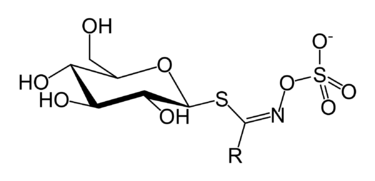
\includegraphics[width=0.25\textwidth]{liugan.png}
	\caption{硫代葡萄糖苷}
\end{figure}

坑埋法去毒,异硫氰酸盐去毒率约90\%,噁唑烷硫酮去毒率约95\%。
具体做法如下:挖一长方形土坑,将菜籽饼(粕)粉碎后每百kg饼(粕)加水100-200kg,搅匀,倒入坑内,盖土30cm,埋1--2个月即可去毒。该方法关键在于土壤水分要低。一般含水在10\%以下,可
达到90\%以上去毒效果。为此,菜籽饼加水必须在坑外进行,不能将水倒入坑内。此外饼(粕)与水要拌匀,否则脱毒效果不好。
\subsection{棉籽饼脱毒}
棉籽饼,一般农村做饲料用,棉籽饼中含有一种有毒的物质--游离棉酚\footnote{黄色晶体,有三种晶形。有毒,难溶于水,微溶于石油醚,溶于稀碳酸钠溶液、氨水(同时缓慢分解)、甲醇、乙醇、乙醚、氯仿、二甲基甲酰胺。}。目前主要采用硫酸亚铁--石灰水溶液进行脱毒处理。可使棉籽饼中游离棉酚含量下降70-90\%。
\begin{figure}[H]
	\centering
	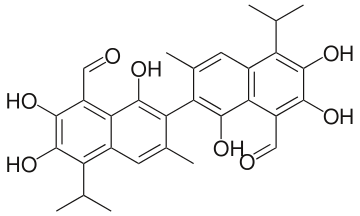
\includegraphics[width=0.3\textwidth]{mianfen.png}
	\caption{棉酚}
\end{figure}

操作方法:

配置硫酸亚铁--石灰水溶液:处理机榨棉仁饼时,每一百kg水加硫酸亚铁200g和石灰粉1--2kg,搅拌,使硫酸亚铁溶解。处理土榨带壳棉籽饼时,每1百kg水加硫酸亚铁400g和石灰粉1--2kg并溶解。

将棉仁饼或带壳棉籽籽充分搅拌。

浸泡:棉籽饼加硫酸亚铁-石灰水溶液(上清液)浸泡2小时到4小时,即可将饼连同泡液一起与其它饲料掺和喂猪。

\chapter{肉鸡鸭鱼蛋加工}
\subsection{金华火腿}
金华火腿之所以在色、香、味方面独具一格,首先是因为采用了“两头乌”优良猪种,它饲养期短,肉质细嫩,皮薄,爪细,精多肥少,腿心饱满。

选4.5-18kg重鲜腿,去毛去血污,剔除残留蹄甲,修去腿周和表面不整齐部分,使其呈柳叶形。然后每50kg鲜腿用4kg盐,(腿少时可按此比例折算用盐量),分6--7次上盐,四个星期上完。第一次上盐是为了脱水和排去淤血。第二、三次上盐是为了稳定肉质。肌肉最厚的三个部位(称“三笺头”)必须加重敷盐量。上盐时要揉搓均匀。上过盐后置于腿床上,堆叠12--14层,每上一次盐,腿位要上下倒换一次。腌制一个月时,其表面会积存一层粘糊状血水和油腻混合物,必须去掉。先将鲜腿放在清水池内浸泡,浸泡时间依气候、腿只大小、盐头轻重而定,一般需2小时左右。再将鲜腿放入水中洗刷,洗后用绳子吊起挂晒8小时左右,进行整形(大腿部整成橄榄形,小腿部整得正直、膝踝无皱纹,脚爪部整成镰刀形)。整形后继续曝晒4--5天,晒至皮坚而红亮出油。然后上架发酵。发酵场地必须保持一定温度、湿度,并通风良好。大中小腿分类悬挂在发酵架上,腿与腿间上下左右前后必须保持一定距离,不可相碰。发酵时间一般选在3--8月份,发酵周期一般3--4个月。发酵期限到了即为成品。
\subsection{广式腊肉}
原料选择与修整:选取猪肋条肉,去骨后,切除奶脯,修整成条状。每条重约170克(烘后净重125克);长约36cm,末端不窄于3cm。上部刺一个小洞,穿上麻绳,便于悬挂。修整后,用温水洗去表面浮油,沥干水分。

配料:肋条肉50kg,白砂糖1860克,60度大曲酒855克,酱油310克,精盐930克,硝酸盐25克。

腌制:将配料混合均匀后涂擦于肉条表面,堆积于容器内。8小时以后,全部配料都已经渗入肉条内,这时将腌肉分别挂于竹竿上,再移入烘房内烘制。

烘制:烘房内放置火盆,并用灰将明火压住。然后将腌肉连同竹竿挂在烘房木架上进行烘制,并控制温度在50℃左右。烘房内木架分上中下三层,下面一层最好挂当天新腌肉条(距火力最近),中间一层挂前一天肉条,最上面挂前两天肉条。如烘箱内系同一天腌制肉条,则每隔数小时需上下调换位置;以防烘坏。肉条经三天烘制即可成为腊肉成品。如不用炭火烤,在天晴时,可在日光下曝晒,晚间移到室内,每天继续曝晒,直至表面出油为止。如曝晒中间遇天阴下雨,应及时送入烘房,用炭火烘烤,不能等天晴再晒。

成品:呈金黄色,每条整齐不带碎骨,味香浓鲜美。

\subsection{香肠}
原料及辅助材料选择:原料肉以猪肉为主,最好选择新鲜大腿肉及臀部肉(瘦肉多且结实,颜色好)。肠衣最好选择26--28mm宽度〈半个圆周)猪肠衣。采用洁白精盐,白砂糖,大曲酒或高粱酒,上等酱油。

切肉:先将皮、骨、腱全部剔去,把肥肉切成小方块,以1立方cm为标准。

配料:介绍几种著名香肠配料标准:

广东腊肠,瘦肉14kg,硝石100克,肥肉60kg,细盐4.4kg,砂糖15.2kg,白酒5kg,白酱油(无添加色素酱油)10kg。

武汉腊肠瘦肉140kg(用绞肉机绞碎),肥肉60kg(切成肉丁),硝石100克,汾酒5kg;细盐6kg,味精600g,白糖8kg;生姜粉600g,白胡椒粉400g。

准备肠衣和麻绳:肠衣用猪或羊小肠衣均可。干肠衣先用温水浸泡;回软后沥干水分待用。麻绳用于结扎香肠。

灌制:将上述配料与肉充分混合后,用漏斗将肉灌入肠内。每灌到12--15cm长时,即可用绳结扎。如此边灌边扎,直至灌满全肠。然后在每一节上用细针刺若干小孔,使烘肠时便于水分和空气外泄。

漂洗:已制成湿肠放在温水中漂洗一次,以除去附着污物。然后依次分别挂在竹竿上,以便曝晒和火烘。

日晒和火烘:香肠灌好后即送到日光下曝晒(或用烘干室烘干)2--3天,再送到通风良好场所挂晾风干。在日晒过程中,若肠内有空气存在时,该部即膨胀,应用针刺破将气体排出。如用烘房烘烤时,温度应掌握在50℃左右,烘烤时间一般为1--2昼夜。

保藏:香肠在1O℃以下温度,可以保藏1--3个月,一般应悬挂在通风干燥的地方。
\subsection{南京香肚}
所谓香肚,是用猪膀胱(尿泡)做肠衣,内装肥瘦猪肉肉馅经过相当时间,就发生香味,可与香肠相媲美。南京香肚,闻名全国,与南京板鸭并驾齐驱。

准备香肚皮子
整理皮子 将新鲜猪膀胱上面管子切去,修去外面所附着筋络肥肉。

盐腌皮子 整理后皮子约重12.5g(2.5钱,1钱=5克(g)),40只皮子约5kg。用500g盐(占皮子重量1/10),分两次擦腌,第一次用全盐量7/10,将皮里外均擦到,然后一个一个放在缸中或坛中,用盖盖好。到第十天时第二次擦盐,即将剩下3/10食盐慢慢擦上去,仍然放回缸中或坛中。经三个月,从盐卤中取出皮子,每一只皮子再用食盐约25g;搓揉腌制,然后放入蒲包中晾挂,可以经过二年左右不变质。盐腌去尿臊味既经济又有效。

皮子装前处理 仔细洗涤,皮子内外各洗6次,即换水12次,洗去附着污物及残余臊味。

装香肚
材料:四六成或三七成鲜猪肉、食盐、白砂糖(不可用黄糖红糖),硝,即土硝(硝酸钾或硝酸钠),香料用八角4份、花椒2份、桂皮1份,用火焙黄,研成细粉。

工具:菜刀、砧板及木盆,切碎及盛放猪肉用。竹签子,粗细如筷子,一头秃、一头尖,长约3.2cm,可以串香肚12只。细麻绳,粗细如穿棉鞋底用麻绳一样;事先断成32cm长,用以收紧香肚口,一根可扣住两个香肚。

材料配合:净猪肉(去骨去皮)100kg,食盐5kg,白糖5kg,香料(三种混合)100g,硝600g\footnote{根据GB 2760-2014规定,发酵肉制品、肉灌肠及西式火腿(熏烤、烟熏、蒸煮火腿),最大用量0.5g/kg,以亚硝酸钠(钾)计,残留量$\leq$30mg。}。

把猪肉切成长约5cm、粗细如筷子肉条,把食盐香料和硝同时加入,充分混合,静置木盆或其他容器内,约30分钟后加糖,再充分混合,15分钟后白糖全部溶化了即可装肚。

装香肚:用有盘秤称取材料,分为200g、250g、300g、350g四种,以200g与250g最为普遍。配料置于大搪瓷浅盘中。手拿皮子,用左右手中指与大拇指捏住皮子边缘,向外一翻,肚口张开对着肉堆,左右手大拇指把肉块很快推进到肚口里。右手握住装肉小肚上部,轻轻向桌面上歪揉同时用竹签在四周刺12--15针以放气,再在桌面上歪揉半分钟到一分钟,将肉内空气全部排出。用竹签封口,约5--7针,后用细麻绳打一个活扣子套在肉肚球形上面与竹签中间,用力拉紧,使肚口收缩,再砍去竹签一段,一个肉肚就脱离竹签;肉肚封口处挂着绳头,照前法再扣上另一个肉肚。

适合做香肚季节:农历十月至次年二月均可。但以十二月份为最好。一般香肚保存6--8个月为好。

香肠后处理:

日晒 冬季日晒3天,一、二月份仅需2天。

晾挂 晒后香肚挂在通风干燥的房间里天花板下面,成串,每五寸即有一个香肚。从一月挂到五月。

叠缸 把晾挂的香肚每4只扣在一起,一层一层地叠在缸中,然后每100只用麻油1kg浇到上面,再行搅拌,使每只香肚外表均涂上薄层麻油,然后把缸盖盖上。

灌肠

灌肠加工方法是国外传入的,但在配料和制造方法上已与原来不同。

原料肉选择 灌肠所用原料肉比香肠范围广,除以猪肉和牛肉为主外,羊肉、兔肉和马肉等都可应用。中等肥度猪肉或牛肉瘦肉。选肉除了要求新鲜外,还必须注意肉结着力,因此,常将原料肉用硝石与食盐在2--3℃低温下腌制48小时。

切肉及腌肉:原料肉选好后,剔去骨胳、筋腱等,将瘦肉切成长约10cm、宽5--6cm、厚2cm肉块(每块约100g),然后用肉重3--5\%食盐和盐量1/20硝石与肉块搅拌均匀,盛入木盆中,置于3--4℃低温下腌制2--3天。腌制时瘦肉和肥膘应分别进行。

制馅:
绞碎肉块 瘦肉腌制完成后用绞肉机绞碎。大多要求用带有2--3mm直径圆眼筛板进行绞碎。

剁碎 将碎肉再进行一次剁碎(一般用旋转剁肉机)。为了防止剁肉过程中温度上升,可添加食用冰和定量冷水。

肥膘切块 将肥膘腌制好,切成0.4cm、0.6cm、0.8cm或1cm大小肥肉丁。

拌馅 将肉馅和肥肉丁、调味料及其他辅助材料用拌馅机充分混合。煮灌肠类和半熏煮灌肠类,在拌馅时还要加适量冷水,以增加肉馅粘性。某些灌肠需加入淀粉时,应将淀粉用清洁水溶解除去杂质后在加肥肉丁前加入。

几种灌肠配料比例:

格拉布斯 瘦猪肉60斤,肥猪肉40kg,牛肉100kg,淀粉20kg,蒜600g,黑胡椒粉200g。

茶肠 瘦猪肉66kg,肥猪肉44kg,牛肉90kg,淀粉10kg,味精100g,黑胡椒粉300g,蒜斤400g。

西班牙 瘦猪肉70kg、肥猪肉50kg,牛肉80kg,淀粉12kg,胡椒400g。

灌制:灌肠品种不同,所用肠衣也不相同,灌制前需按规定准备好肠衣,并按规定方法进行结扎。灌制方法基本上与香肠相同。

烘烤:选择少树脂木材(如柞木、椴木、桦木、榆木等),交叉摆在炉内,引火燃烧.待炉内温度已达60--70℃,再把灌肠摆放到炉内烘烤。烤炉内灌肠从下垂一端算起,距火苗必须在60cm以上。每烤5--10分钟将灌肠上下或里外调换一次。炉温应保持65--85℃(以下层灌肠尖端温度为准)。在此温度下,粗灌肠45--80分钟,细灌肠25--40分钟即可烤好。

煮制:一般用水煮。水温85--90℃时下锅,保持温度在78--84℃。羊肠衣灌肠煮制10--15分钟;牛和猪小肠灌肠煮20--30分钟;牛大肠灌肠煮35--45分钟;粗牛大肠和羊拐头(盲肠)灌肠煮35--55分钟;牛拐头灌肠煮100--120分钟。用温度计插入肉馅中观察,如灌肠中心达到72℃,说明已煮好,可即出锅。如制造湿肠,冷却后即为成品。

熏烟:目的是除去灌肠部分水分,肠衣亦随之变干,肠衣表面产生光泽并使肉馅呈鲜艳红色,使其具有熏香味和一定的防腐能力。煮制灌肠在35--45℃的温度下熏12小时左右,半熏煮灌肠在35--50℃温度下熏12--24小时,生熏灌肠在18--22℃下熏5-7昼夜。
\subsection{肉松}
肉松是以瘦肉除去水分而制成,所以猪肉、牛肉、鸡肉等瘦肉都可以加工成肉松。

原料肉处理:除去骨、皮、脂肪、筋腱及结缔组织等,然后将瘦肉顺其纤维纹路切成肉条后再横切成3cm长短条。

配料标准:随各地习惯而不同,仅举一例:瘦肉100kg,酱油44kg,白糖3kg,黄酒4kg,茴香120g,生姜1kg。

煮肉及炒干:把瘦肉放在锅中,加入与肉等量清水,然后分三个阶段进行加工。

第一阶段 把肉煮烂。用大火煮沸后,撤去浮沫直至肉烂为止。如肉未烂而水已干时,可以酌量加水。当用筷子夹肉,稍加压力,肉纤维即自行分离,则表示肉已煮烂,此时可以把调料加入,并继续煮至汤快干时为止。

第二阶段 即炒压阶段。用中等火头,一边用锅铲压散肉块,一边翻炒。注意不要炒得过早或过迟。因炒压过早,肉块未烂,不易压散,工效很低;炒压过迟,肉块太烂,容易焦糊,造成损失。
第三阶段 即炒干阶段。火头要小,连续勤炒勤翻,操作轻而均匀,在肉块全部松散和水分完全炒干时,颜色就由灰棕转变成灰黄色,成为有特殊香味金黄色肉松。

将刚加工肉松趁热装入玻璃瓶内,瓶子预先洗涤、消毒和干燥,放在干燥处,可以保存六个月不变质。装入防潮纸或塑料袋内,亦可作短期贮藏。
\subsection{肉干}
肉干是用新鲜瘦肉加入配料切碎制成,其原料多采用牛肉,且以新鲜前后腿瘦肉为最好。

原料处理:先将原料肉脂肪及筋腱除去,然后用清水把纯瘦肉洗净沥干,切成3cm左右肉块。

水煮:将肉块放入锅中,用清水煮30分钟左右,当水刚烧开时,撇去浮沫,捞出切成肉片或肉丁。

配料:根据各地习惯而定。介绍几种配料方法供选择。

第一种 瘦肉100kg,食盐2.5kg,酱油5kg,五香粉250g(或将茴香、陈皮及桂皮适量包扎于纱布内,投入锅内与牛肉一起煮)。

第二种 瘦肉100kg,食盐3kg,酱油6kg,五香粉200--400g。

第三种 瘦肉100kg,食盐2kg,酱油6kg,白糖8kg、黄酒1kg,生姜250g,葱250g,五香粉250g。

复煮:取一部分原汤加入配料,用大火煮开。当汤有香味时,改用小火,并将肉放入锅内,用锅铲不断轻轻翻动,待汤汁快干时,即将肉片取出并沥干。

烘烤:将肉片平铺于铁丝网上,用火烘干即为成品。烘烤时,烘房温度应保持在50--55℃,并需经常翻动肉片,避免烤焦。

如在烘烤前,肉片中加入其他香料时(如五香粉、辣椒粉和蚝油等)也同样处理。
\subsection{湖南坛子肉}
湖南坛子肉是湖南瑶族和山区汉族人民传统食品,具有独特风味。

脆渍方法是:冬至到次年立春前,选用三成肥、七成瘦鲜猪肉,带皮剔骨,严格按比例投料.可以腌渍成不同风味坛子肉。

(一)米粉坛子肉

将生肉洗净上挂,沥干水分,切成薄片,盛在木盆或瓷盆里,分层投加适量食盐、酱油、烧酒、红糖,腌渍3--5天,使其浸透均匀,燃后分块粘上五香米粉,置于篮席或钢丝筛上,用木炭小火连续烘烤48小时,严格掌操火候,待其开始冒烟,使米粉肉两面色泽金黄,冷却后,装坛加盖密封。

(二)油炸坛子肉

生肉切成四方块,加少量生姜,一同下锅煮沸,三成熟即可,趁热捞出浸泡糯米酒,加红糖150g,用葱汁水擦在肉皮上,以烧沸茶油炸熟,使肉质柔软、皮脆、色黄。冷却后,成块装在坛子里(也可切成二指宽厚薄片),配辣椒酱、大蒜头搅拌均匀,装隹密封。

坛子要干净不漏气,密封后要放在干燥通风的地方。

食用方法:
米粉坛子肉,可配蒸土豆(马铃薯)或槟榔芋,以食盐、酱油、味精、香料等为佐料,上笼蒸熟,使其滋润溶合,余香久留。

油炸坛子肉,可做扣肉,配蒸盐菜,拌少量生姜末,下锅炒一下,投下油、盐、味精、香料后出锅,将肉切成连片放在盘底层,肉皮向下;上面加盐菜,上笼蒸烂,倒翻入碗。也可拌豆豉和辣椒酱,或切成肉片配青菜小炒,亦可淋上酱油、麻油凉食。
\subsection{风鸡}
材料:公鸡或母鸡,食盐,花椒或肉桂。

腌制过程:鸡在屠杀前12--24小时不喂饲料,仅给清水。如此,则出血干净,肉质比较新鲜。

在喉部放血,嗦囊处用刀割一小口,取出剩留食料。在泄殖腔下边割一个长约5cm直形口子,同时剜去肛门。用右手第二第三指伸入腹腔,轻轻拉出所有内脏。嗦囊也同时带出。

每只鸡(已去内脏)重500g,用食盐29g,花椒粉5g,互相混合后,以手擦入腹腔,并将食盐花椒混合物放入口中,喉部,以及嗦囊伤口。

盐擦好后,把鸡背放在桌上,两腿依自然姿势向腹部压下。再将鸡头拉到左翅下(方便操作)。

将尾羽向上,压到腹部,随即用左右两翅包住,然后用细麻绳纵横束起。

用较粗麻绳扣住鸡体,背向下腹向上,挂在屋檐下或天花板下风干。风干处条件是:无直接日光,相当通风,干燥而凉爽,愈高愈好。

半个月即可腌透。一个月就可取食,风味别致。
\subsection{板鸭}
板鸭制法各地有所不同,主要不外单独以盐腌及调味浸腌两种。
(―)盐腌鸭
鸭于宰杀、煺毛、剖腹除去内脏,切去翅尖脚爪,洗净血污,晾干表面附着水分,再用10\%食盐将鸭肚内外擦遍;于是放入缸中,上压重石,约经7天,即可腌成。

气温高时时间缩短。在腌制期间,须上下翻转1--2次,同时在腹腔及颈口部分或有欠缺之处补充食盐。腌成后先晒3--5天,至适当干燥后,移至通风处风干。

(二)调味浸腌鸭

即板鸭普通制法。宰杀鸭子褪毛、除去内脏后洗净并沥干余水,用花椒炒食盐,遍擦肚内外,腌6--7小时,淋去血水。层层用卤液浸润,有些每层间隔以荷叶,上加木板,压以重石、卤液以淹没鸭层为度,每隔2--3日翻动一次,随气温高低不同约经5--10日、即可取出晾晒,以至风干,即为成品。我国著名的南京板鸭,多在小雪后制作,可以经年不坏,且不失原味。

配制卤液,用水量约为鸭肉净重的50\%,盐为10--15\%,以及适量香辛料。香辛料种类与数量并无一定标准;如腌10只大肥鸭,其配料是:大茴香11.3g,小茴香及桂皮各3.8g,陈皮7.5g,丁香1.2g,老姜37.5g,绍兴酒(或黄酒)1.2kg,另加硝石18g。先用水抽煮各香辛料有效成分,再与酒及硝石混合溶解备用。
\subsection{油淋鸡}
湖南特产,由挂炉烤鸭演变而成。

选用当年1kg左右肥壮小母鸡(乌鸡不能用),宰杀去毛并洗净,平放案板上,鸡头朝本人,左手将右翅提起,连同鸡颈抓在一起,右手持一尖刀,从右翅胁下处开二小孔(刀先横,然后提直朝上划去)约八分大,刀口朝翅膀那边,从二关节切断翅、足。用右手大拇指插入开口内,将心肝按下去,再用食指将食袋(嗦囊)和气喉管带出,然后食指又插入小孔,将肝往后压,手抵肛门,将鸡肫子往前推移,继而将肫、肝、心连同肠子一并取出,控净肺叶,漂洗,沥干水分。用7cm长(2寸)、16mm(5分)宽木片插入胸腔,将胸背撑起,投入开水锅内,把鸡皮烫伸,用抹布抹干鸡身水分,取少许稀饴糖放在手心,从上到下,左右两边,将鸡擦匀。用细竹简一根(切斜口)插入鸡双腿吹气后,进烤房将鸡胚烤干,表皮起皱纹即可。用5cm(1.5寸)竹签将两翅撑起。用小木塞将鸡肛门塞紧。用小铁钩将鸡颈窝成圆形挂起。备铁锅一只,将茶油烧开,左手拿铁钩将鸡提起,右手用小铁勺舀油,反复往鸡身上淋,先淋鸡胸、鸡腿,次淋鸡背、鸡头,肉厚的部位要多淋几勺油。油温掌握90℃左右(油温过高,会使鸡皮起壳皮糊而里面难熟),大约淋8--10分钟,鸡身呈金黄色带亮,有皱纹,说明鸡已淋熟。取出竹片和木塞。如肚内流清水,证明已熟,如流浑水,证明未熟,必须再淋几遍,方为成品。

食用方法:

凉食,将鸡切片、切块,做拼盘,加姜末加葱,淋上芝麻油和酱油,即可食。

炒食锅放猪油100g烧开,将一只鸡切成13.3--16.7mm(4-5分)宽,3.3cm(1寸)条块,与100g花生米一起下锅炸,把姜25g(1钱)、绍酒50g(1两)、优质酱油50g(1两)、青椒100g(2两)及少许味精、蒜等投入锅内搅动,出锅淋芝麻油,即可食。
\subsection{皮蛋}
皮蛋又叫松花蛋、变蛋、彩蛋等。加工方法很多,现介绍滚粉法制作皮蛋技术要点。

原料蛋选择:选用新鲜鸭蛋,要求蛋白浓厚澄清,蛋黄位于中心,照视时无蛋黄暗影,蛋白无任何斑点及斑块。

辅料选择:滚粉法仅用碱粉(碳酸钠)、生石灰、食盐三种辅料。市售碱粉中,常有食碱(或称洗碱块〉,如用此种碱块为材料,应先经过加热脱水成为干粉,按配方称取重量。制皮蛋用生石灰应选用新出块状石灰。食盐最好应用精盐(细盐),如无精盐,可将粗盐研成细粉后用。

用料量:滚粉法每100只鸭蛋,用碱粉100g、生石灰100g,食盐50g。是中等大小鸭蛋用料,如为大鸭蛋,用料量可酌量增加。

消化生石灰:生石灰加水消化,以每100g生石灰加水35g为合适。加水时要均匀。

滚粉与密封:将石灰粉加入碱粉100g(要不结块),精盐50g混合均匀即可使用。如放入小铁锅中,用锅铲混合均匀,锅下生火,使混合粉呈高温状态备用更好。此混合粉可供滚制中等大小的鸭蛋100只用。另取一盆清水,取粘土适量,放入搅和,使成稀薄泥浆。先把鸭蛋放入泥浆中浸湿,使蛋壳表面粘上一层薄薄泥浆,然后把蛋放入混和粉中滚动,使全蛋的表面都粘上一层薄粉。蛋滚好粉后,随即放入坛中,坛口立即加盖用泥密封;或用双层塑料布扎坛口。如用塑料袋盛蛋,扎好袋口,密封不透气也可以。

制皮蛋以春天最合适。鸡蛋也可做皮蛋;用碱量较多,每100只鸡蛋需用碱粉150g、生石灰150g、精盐50g,制作手续及注意事项与鸭蛋同。

将皮蛋放在手中颠动,有震动感者即已成熟。
\subsection{咸鸭蛋}
咸鸭蛋腌渍最常用方法有盐泥涂布和盐水浸泡法。
(一)盐泥涂布法

材料配合:鸭蛋100个,食盐1.2--1.5kg,干燥黄土1.3kg,冷开水0.8--0.9kg。鸭蛋少于或大于100个时,可按上述配比比例折算材料用量。

加工方法:将食盐放在木桶中,加清水使其溶解后,加入黄土用木棒搅和,使其成浆糊状。泥浆浓厚程度可用鸭蛋试验,即取一个鸭蛋放入泥浆中,如有一半浮在泥浆上面,则表示泥浆浓厚程度最合适。

新鲜鸭蛋通过照验、整理、敲验三道工序后,放在泥浆中(每次3--5个),使蛋壳上全部粘满盐泥,再将蛋放入缸或箱内,并清点蛋数。加工高邮咸蛋时,涂泥后还要滚灰,使盐泥蛋面附上一层薄干草灰,使蛋与蛋之间相互不粘连,然后点数入缸。把剩余泥料倒在缸中咸蛋上面,盖上缸盖即可。咸蛋成熟时间,春秋两季一般约需30--40天,夏季只需20天左右。

(二)盐水浸泡法

腌制方法:把食盐放入容器中,倒入开水使食盐溶解。待冷至20℃左右时,即可将蛋放进去浸泡。盐水浓度以20\%为宜(即2kg食盐加8kg开水),夏季盐水浓度可以略为提高。
\subsection{鱼粉}
鱼粉可分为食用鱼粉和饲料鱼粉,目前生产最多还是饲料鱼粉。

原料:饲料鱼粉加工原料,一种是低级鱼类或者变质鱼类,另一种是鱼片、鱼罐头加工中废弃物,如头、鳍、内脏等废料。

加工方法:

蒸煮 将原料放入蒸煮锅中加热煮(蒸)熟。小型土法加工可以用大铁锅或蒸笼等简单设备。

压榨 处理完毕后原料放入压榨器内加压,使鱼肉组织中部分水分和油脂一起流出。土法生产可以用杠杆式简单压榨设备。

干燥压榨后半制品经过干燥使水分减少到10\%左右。小型土法生产可用日干。但遇到雨天容易腐败时候,仍需用简单烘干设备。

磨粉:充分干燥后半制品进行磨粉;粉粒大小一致均匀,用筛筛过。小型土法生产可用石磨。

包装和贮藏 制品一般用麻袋等包装贮藏。贮藏中应防止吸潮和油脂氧化发热而引起着火。
\subsection{龙虾片}
龙虾片是用鲜鱼肉掺淀粉及调味料经蒸熟后冷却切片、干燥所得制品。食用时采取油炸、沙炒、爆筒加热膨胀,成品酥松香脆、鲜美可口。现介绍浙江宁波地区加工方法作参考。

原材料:

选用新鲜带鱼,去头尾、内脏,用清水洗净,取其净肉重50\%左右上等淀粉。

配料:淀粉90kg,鱼肉10kg,味精1kg,砂糖3.3kg,精盐2.3kg。香料水(桂皮500g,甘草500g,八角500g)熬汁至2kg。另用淀粉16kg加水38kg(打浆用)。

原料调配:

味精用水化开再加入。淀粉打浆用水化开化匀,再用蒸汽吹,边吹边搅拌,关键要烫手、要稠,待透明状即可。如要加工彩色鱼片,可加入适量食用色素。

打浆搓条:把原料、调味配料与浆粉同时放入打浆机内,再把热浆逐渐加入,约打浆20分钟,待均匀后,即可取出,倒入木箱中,用布盖好保温,然后分次在木板桌上搓条子,要求搓得结实,中间不得有微孔,条子粗细一般直径5cm为宜。

蒸煮:把条子排列在蒸箱架上约蒸煮1小时,然后放在桌板上冷却12小时。

冷却切片:把冷却条子放进0--2℃预冷库内约30小时,待发硬至棒状即可用切片机切片,厚度为1mm。

干燥:将鱼片用风吹、日晒或烘房烘干即为成品。
\subsection{五香烤鱼}
备料:

原料选择要求鲜度较好、条形完整的小带鱼或小杂鱼。将原料鱼去头尾、内脏,小带鱼切成7cm长条块,小杂鱼以去头整条为宜,用清水洗净后在波美8度盐水中浸泡5分钟,沥水后即可。

拌腌香料水制法:八角400g、桂皮400g、茴香400g、花椒400g、姜片400g,洗净敲碎,加水24kg,煮熬至12kg(约1--1.5小时)。过滤后可以配制100kg鱼块(如鱼块多则香料水按比例增加),然后在过滤液中加白糖5kg,酱油6kg,精盐3kg,黄酒3kg(最后加入防止挥发)。

过滤后剩余残渣,可用上述五种香料各200g,再放24kg水,连渣一并煮熬,使成12kg,可作第二次配料。

蒸煮将鱼块平摊在铅丝\footnote{推荐使用钢丝。}架上用蒸汽吹熟。

烤干蒸煮后放进温度80℃烘房内烘烤7--8小时,待6--7成干后取出,在香料水中浸泡30分钟,并不断搅拌使受料均匀。将浸透香料水鱼块第二次进烤房烘烤4小时,待九成干后即为成品。
\subsection{熏鱼}
用作熏鱼原料多为青鱼、草鱼、鮸鱼等中型鱼类,也有用鲤、鲢、鲳昌等鱼,但以青鱼为最好,其条重以5kg左右为宜,活鱼更理想。

原料处理:原料用清水洗净后,刮净鱼鳞,剪去鳍条。然后剖腹挖去鳃及内脏,切不可挖破胆囊\footnote{某些鱼类胆汁有毒,包括草鱼、青鱼、赤眼鳟、鲫、鲤、鳙、鲢、鲮、圆口铜鱼、似刺鳊鲌、翘嘴鲌、团头鲂,胆汁均具有一定毒性。不论生吃、熟食、泡酒吞服、还是以鱼胆汁滴眼等外用手段,都会引起中毒,且中毒程度跟服用剂量正相关,严重者危及生命,并可能造成死亡。胆汁中毒性物质鲤醇硫酸酯钠能耐高温、耐酸,不易被胃酸、乙醇所破坏,组胺、氢氰酸、胆酸等也会对人体组织造成损伤。胆汁有毒鱼类统称为胆毒鱼类(Gall-bladder poisonous fishes)。部分鱼类鱼胆苦味重,影响食用。}。再用热净布(热水中洗净拧干)擦去腹腔内血污、黑膜等。切下鱼头,纵劈为两片,跟鱼块同样加工;胴体则沿脊骨背开成两条鱼片(一条带脊骨,一条不带脊骨)。如鱼片较大,应分别剖出两条肚肉,并可切成适当长度,跟鱼块同样加工,唯浸渍、油炸时间应相应缩短些。将鱼片横斜切成皮面约1--2cm左右(即鱼块厚度)的斜刀块,大小厚薄均匀。带脊骨和不带脊骨鱼块应分开放置(浸渍及油炸时间,带脊骨的鱼块稍长些)。

浸渍浸渍用料为精盐和红酱油。一般100kg鱼块加入4.5kg酱油溶液、(3kg红酱油,1.5kg精盐),搅拌均匀后,夏季浸渍1.5--2小时。

\textcolor{red}{下页内容缺失。}
\chapter{面食制作}
\section{蒸食类}
馒头、花卷、发糕,品式极多。具有松软暄绵,香甜可口,易于消化等特点,是面食主要品种。

馒头、花卷、发糕在制作和成熟过程中,需掌握关键在于发面、对碱、火候。

不同面粉;温度与发面时间和用碱量有直接关系。一般说来,面粉湿度大,气温高,发面时间要短;反之,面粉湿度小,气温低,发面时间则长。面含酸量大,用碱要多:面的含酸量小,用碱则少;发面方法科学,不用老肥发酵,对碱除酸,而用发酵粉最好,因为发酵粉能保持面粉中营养成份不致破坏。

怎样验证发酵面用碱量是否适宜,可参考下列方法:

1 嗅,闻不出异味,即碱量适宜,有酸味即碱小;有碱味即碱大。

2 拍,提起面团拍击,发出膨膨声即碱量适宜;噗噗声即碱小;实死声即碱大。

3 看,面团切开,剖面蜂窝眼大小匀称,为碱量适宜;蜂窝眼大而不匀为碱小;蜂窝眼扁,面发死,色发黄,为碱大。

4 揉,手感有弹性,面不粘,面团光滑为适宜;弹性小,发粘,没有劲,为碱小;面团实板死,有劲,为碱大。

5 触,将面团切开,剖面相对接触,似沾而不沾为适宜;粘而沾为碱小;不沾为碱大。

6 尝,从软面团揪少许面胚,嘴嚼有酒香或面香味为适宜;有酸味为碱小;口感凉而涩为碱大。

不适宜碱用量处理:

1 碱大,可再加水面和少许面肥,揉匀即可。

2 碱小,可再对入适量碱,揉匀,醒透即可。
\subsection{开花馒头}
1 老面肥发酵足透,分次对入干面粉揉匀,稍醒,对碱,揉透,加白糖,揉匀成面团。

2 面团搓条,1斤面揪10个剂,剂口朝上,呈自然花瓣形,摆于屉中。

3 上旺火蒸约15分钟,即可出锅。
\subsection{呛面馒头}
1 将干面粉徐徐揉入老面肥中(1斤面肥需5两干面)对碱,揉匀成稍硬面团,醒透。

2 面团搓条,1斤面揪10个剂,揉匀成圆形馒头;

3 将馒头摆于屉中,用旺火蒸约20分钟,即可出锅。
\subsection{桂花馒头}
1 面粉放容器中,上屉蒸熟,取出晾凉,擀碎,过箩。

2 鸡蛋清、黄分开。蛋清抽打成蛋泡糊。蛋黄加入白糖、桂花搅匀。然后将蛋清、蛋黄和在一起掺匀,对入熟面拌匀。

3 小碗逐个抹层猪油,然后放入青红丝、元肉\footnote{桂圆肉,又称“龙眼肉”“元肉”。桂圆是无患子科龙眼属常绿乔木龙眼树成熟果实,可食部分为假种皮,一般干制保存,即龙眼肉。},再把和好面
糊装入多半碗,上屉用旺火蒸约15分钟,即可取出。

用料比例:1斤面粉,1斤鸡蛋,1斤白糖。青红丝、元肉、桂花适量。
\subsection{杠面高桩馒头}
原料

面粉1斤(包括酵面1两)。

做法

将面粉三两、酵面一两、凉水三两调和成面芡发酵,发起后往回落时,再呛进干面粉六两揉成面团。上杠子压出光面,下成剂子(一两一个),用手搓成二寸高馒头坯子,将坯子放倒用布盖上,放在暖和地方,醒一会儿后,再翻过来醒一会儿,四面都醒好。

2.屉格钉上一寸二分高的竹签,把馒头插在竹签上,用急火蒸十五分钟即熟。

质量标准

出屉后,成品色泽洁白,个头均匀,微甜干香,耐嚼力强。
\subsection{肉丁馒头}
原料

精粉1斤(包括酵面2两〉、猪肉8两、大慈5两、姜末1钱、 花椒面1分、酱油1两;面酱5钱、猪油5钱、芝麻油一3钱、腐乳0.5 块、味精2分、食碱适量。

做法

1.把猪肉切成二分见方小块。葱切成葱花,猪肉丁加入酱油、面酱、猪油、腐乳拌匀,再加入葱花、姜末、味精、芝麻油拌匀成馅。

2.将精粉与酵面加入食碱揉匀,醒一会儿。搓成长条,下成三十个剂子,擀成圆形皮。

3.左手拿皮,右手拿竹匙子抹馅,双手合拢包成包子,再装入带花纹模子里卡一下取出花纹向上,摆在屉内蒸熟即可。

质量标准

出屉后,成品色泽洁白,外形带花纹,个头均匀,吃之鲜香。
\subsection{长条花卷}
原料

面粉1斤(包括酵面5两)、芝麻油2钱、花椒盐1.5钱、食碱适量。
做法

1.面粉加入温水和好,放入酵面揉匀,酵面发起时再加入食碱揉匀。

2.用大走槌擀成一分厚方形片,刷上一层芝麻油;撒点花椒盐,由外向里叠卷起,成扁圆形,切成十个同样大长方形剂子,双手捏住两头抻三寸左右长,双手向两个方向拧两个劲,即为长条形花 卷,摆在屉内蒸十分钟即熟。

质量标准

色泽洁白,形状整齐,层次清楚,薄厚均匀,暄软可口。
\subsection{重样卷}
1.发酵面对准碱,揉匀成面团。

2.面团擀成大圆片,将一半刷油,撒糖、青、红丝;另一半抹匀果酱。两面分别向里卷起,卷好后翻过来,切成1斤面5段,摆于屉中。

3.用旺火蒸约10分钟,取出后中间切开即可。
\subsection{脂油卷}
原料

精粉1斤,(包括酵面5两)、猪板油2两、大葱1两、芝麻油2钱、精盐2分、花椒面1分、食碱适量。

做法

1.将精粉用温水和好,加入酵面、食碱揉匀,醒一会儿。

2.把猪板油去硬皮,切成小丁。葱切成末。加入精盐、花椒面、芝麻油拌匀成馅。

3.将面揉匀,擀成一分厚长方形片,把脂油葱花馅抹在面片上并抹匀,由外向里卷起来,用刀切成十个同样大小剂子,用双手捏着两边向相反方向拧上两个劲,然后立起来,一头按在案子上,上头用大拇指往下按,成螺旋式,逐个做完。

4.屉内铺屉布,把生坯摆在屉内,蒸十分钟左右,成熟取下即可。
\subsection{金银花卷}
原料

精粉1斤(包括酵面2两)、蛋黄5个、豆油2钱、食碱适量。

做法

1.先将六两精粉加酵面和好发酵。

2.再将四两精粉加蛋黄和好揉匀。

3.将已发好酵面加碱揉匀,擀成长方形薄片,刷上—层豆油,再把和好的蛋黄面也擀成同样大的片,摞在上面,再刷一层豆油,边沿整齐,由外往里卷起,搓细。

4.用刀切二十小段,刀口向上,两段合在一起,用筷子由中间夹一下,成为花卷生坯,上屉蒸熟即成。

质量标准

黄白分明,层次清楚,个头整齐,暄软适口。
\subsection{豆沙卷}
原料

精粉1斤(包括酵面5两)、豆沙馅5两、豆油5钱、食碱适量。

做法

1.将精粉用温水和好,加入酵面揉匀,醒一会儿,使它发起。

2.把发好的酵面加入食碱揉匀,搓成条,下十个等量剂子,每个面剂擀成五寸宽、二寸长片。

3.在面片上刷一层油,抹上一层豆沙馅,从宽面两边对着卷起来,中间抹点水粘住,翻过来整理均匀。

4.将生坯摆在屉内,放到锅上蒸熟取下,上桌时由中间切成两段,码盘。

质量标准

色泽洁白,形状整齐,个头均匀,暄软甜香。
\subsection{千层糕}
原料

发酵面(精粉)1.5斤、白糖5两、猪板油1.5两、桂花酱2钱、葡萄干2钱、青梅1钱、红樱桃10粒、熟瓜子仁2分、食碱2钱。

做法
1.将猪板油去硬皮,切成小丁,加入白糖(四两)、桂花酱搓匀,和成脂油馅。

2.将酵面加食碱,加入一两白糖揉匀,擀成二分厚四寸宽长片。将白糖脂油馅,撒在已擀好面片上,从一头叠起,约叠三寸宽,登到头,用手按成八分厚长方形。再把青梅(切片)、葡萄干、红樱桃、瓜子仁分别摆在糕面上按平,即成糕坏。

3.将糕坯摆在屉内.蒸三十分钟左右即熟,晾凉后切成菱形班码盘即可。

质量标准

色泽洁白,层多不破,香甜喧软,味道清香。
\subsection{蜂糖糕}
原料

嫩酵面1.5斤、猪板油2两、白糖3两、蜜枣5钱、背红丝1钱、食碱2钱。

做法
1.把板油去硬皮,切成小方丁。蜜枣切碎。

2.酵面加入食碱揉匀,再将板油丁、白糖放在面内揉匀,放在温暖处发一小时,再放在通风处晾一会儿。

3.把晾面擀成五寸见方小块放笼屉内,撒上蜜枣、青红丝。用旺火蒸二十五分钟成熟取下即可,凉后切块码盘上桌。

质量标准

色泽洁白,暄软,蜂窝多,香甜适口。
\subsection{黄糕}
原料

熟面粉7两、鸡蛋1斤、白糖1斤、青红丝2钱、瓜子仁1钱、葡萄干1钱。

做法

1.把鸡蛋打开;蛋清与蛋黄分别装入两个盆内。

2.用打蛋器或筷子,将蛋清抽成泡沫状。

3.将白糖擀细倒入蛋黄内抽打,待糖溶化后,再倒入蛋清糊内搅匀,之后再加入熟面粉搅匀。

4.将蒸糕用的木方框放在屉内,铺上洁白布,把蛋糊倒入木方框内,摇动几下,使蛋糊面平整,把青红丝、瓜子仁、葡萄干均匀地撒在上面,用旺火蒸三十分钟左右成熟取下即可。上桌时切成小块。

质量标准

色泽金黄,整齐不碎,甜暄适口。
\subsection{三色糕}
原料

熟面粉7两、鸡蛋1斤、白糖1斤、豆沙馅5两,青梅丝2钱、葡萄干2钱;瓜子仁1钱、食用色素适量。

做法

1.将鸡蛋清、黄分别打在两个盆内,抽成糊。之后,合在一起,加入白糖、熟面粉搅匀。

2.将蛋糊倒入蒸糕木框内一半,蒸熟取出。

3.把豆沙馅擀成与蒸糕同样大小片,放在蒸糕上面。

4.把另一半蛋糊加点色素,调成玫瑰色,倒入豆沙馅上面,再撒上青梅丝、葡萄干、瓜子仁,放在锅上蒸熟取下。晾凉后切成方块。

质量标准

黑黄红三色分明,整齐不碎,暄软香甜。
\subsection{山楂云卷糕}
原料

熟面粉5.5两、鸡蛋10个、白糖4两、金糕1斤。

做法

1.把鸡蛋磕开,蛋清与蛋黄分别放入盘内,把蛋清抽成糊,能立起筷子为止。再把蛋黄抽开,将白糖倒入蛋黄内搅匀,再放入蛋清糊内搅匀,然后把熟面粉放入糊内再搅匀。

2.把蒸糙的木格放在屉内,铺上屉布,把和好的蛋糊,倒入木格内,上屉蒸约十五分钟即熟取出(蒸熟约一分五厘厚)。

3.将蒸糕倒出,取下屉布,把金糕切成薄片,摆在上面(即靠屉布那面),随即用净布把糕卷起卷紧,晾凉后把布打开,顶刀切成二分厚的圆卷形片,摆在盘内即成。

质量标准

形似云卷,整齐不碎,暄软甜酸。
\subsection{千层饼}
原料

精粉1片(包括酵面2两)、豆油5钱、花椒面1分、精盐1分、食碱适量。
做法

1.将八两精粉与二两酵面用温水加食碱和成面团,醒一会儿。

2.将面团揉匀,搓成条,下大小基本相同五个剂子,再擀成一头宽一头窄梯形片。

3.把梯形片逐个刷油,撒上花椒盐面,由窄头卷起来,用宽头将两面包好,再擀成椭圆形片,用刀背在饼上交叉压上菱形花纹。上屉蒸熟取出,由中间切开为两片即成。

质量标准

色泽洁白,形似牛舌,层多暄软,味美可口。
\section{烤食类}
\subsection{香蕉酥}
原料

精粉1斤、蛋黄2个、白糖3两、豆油2两、枣泥馅3两、香精1分。

做法

1.将精粉倒在案板上,加入豆油、白糖、香精拌匀,用温水和好揉成软面团,搓成长条,揪成二十个剂子按扁。

2.将面剂逐个包进枣泥馅,搓成两头细中间粗的香蕉酥生坯。

3.将香蕉酥生坯放烤盘内,再把蛋黄用筷子搅匀,用刷子往香蕉酥上面刷一层蛋黄,放烤炉内烤七八分钟成熟取出即可。

质量标准

色泽金黄,形似香蕉,光亮整齐,不破皮不漏馅,香甜适口。
\subsection{混合糖稣}
原料

精粉3斤、猪油1斤、鸡蛋1斤、白糖1斤、芝麻2两、葡萄干2两、桂花酱1两、香精适量。

做法
1.把芝麻洗净炒熟待用。将鸡蛋磕在盆内(留出两个鸡蛋待用)。把白糖、猪油、葡萄干、桂花酱、香精加入鸡蛋内搅匀,倒入精粉内和匀,揉成面团。

2.把面团搓成条,下三十个剂子,擀成圆形饼状。或用各种花样模型,磕出成型。

3.把两个鸡蛋打在碗内搅匀,用刷子逐个把饼刷上一层蛋液,再撒上一层芝麻。

4.把生坯摆烤盘内,放入烤炉烤十分钟左右,成熟取出即可。

质量标准

色泽金黄,形状整齐,不破边不裂劈,香酥整甜,口味多样。
\subsection{玫瑰冰花酥}
原料

精粉1斤(包括熟精粉1两)、猪油4两、白糖4两、玫瑰酱5钱、青红丝1钱、冰糖1两、香精适量。

做法

1.将白糖加入熟精粉、玫瑰酱、青红丝、香精、猪油(五钱)拌成馅。

2.用五两精粉、二两五钱猪油擦成干油酥面,分成十块。

3.再将四两精粉加猪油用温水和成水油面,揉匀分成十块。

4.用水油面逐个包进干油酥面,擀成椭圆形后,从两边往中间叠,叠三层,擀成长条,由外往里卷起来。两头窝起按扁,逐个包上三钱糖馅,擀成直径二寸五分圆饼。上烤炉用慢火烤二十分钟左右取出,用一两白糖熬成糖水刷在表面上,把冰糖擀成碎渣撒在上面,再入炉烘干即可。

质量标准

杏黄色,圆形,酥脆香甜。
\subsection{开口稣}
原料

面粉1斤、白糖2.5两、猪油4两、小苏打少许。

做法

1.将五两面粉,加二两五钱白糖、三两猪油,再加入小苏打和成油酥面。

2.将五两面粉加一两猪油拌匀,用温水和成水油面,揉成筋性面团。

3.用水油面包进油麻面,擀成长方形片,叠成三层,再擀成长方形片,卷起来搓匀。用刀切成相同大小剂子,把剂口包严捏紧,揉成椭圆形按扁。再用刀在表面上斜切成井字形,摆入烤盘内,入炉
烤十分钟,成熟取出即可。

质量标准

色泽金黄,层次分明,酥脆香甜。
\subsection{白皮酥}
原料

精粉1斤(包括熟精粉1两)、猪油4两、白糖3两、青红丝1钱。

做法

1.用四两精粉加猪油(二两)擦成油酥面。其余精粉加猪油(一两)用温水和成水油面。

2.将白1糖、青红丝(切碎)加猪油(一两),用熟精粉搓成馅。

3.用水油面包进油酥面;再用面杖擀成长方片,切齐边沿,往里卷起抻长,下二十个剂子。

4.将剂子按扁,逐个包上馅,再擀成圆饼,中间点一红点。

5.摆入烤盘,放入炉内烤,见饼面硬时取出,盖一层纸或盖烤盘,用慢火烤熟即可。

质量标淮

形圆,皮酥色白,甜香适口。
\subsection{白皮豆沙酥}
原料

精粉1斤、豆沙馅4两、猪油3两。

做法

1.用四两精粉加猪油(二两)擦成油酥面。用六两精粉加猪油(一两)、温水和成水油面。

2.用水油面包进油酥面,再用面杖擀成长方形片,切齐边沿,往里卷起抻长,下二十个剂子。将剂子按扁,每个包入豆沙馅(二钱)按一下,再擀成直径一寸五分圆饼。

3.将饼坯放入烤盘内,入炉烤至见饼鼓起,皮稍硬时,将烤盘上面盖上铁盘,再用慢火烤熟即可。

质量标准

形圆,个头匀,层次分明,色白酥甜。
\subsection{一品酥}
原料

精粉3斤(包括熟精粉1两)、豆油4两、白糖3两、熟芝麻8钱。

做法

1.用四两精粉加豆油(二两)擦成油酥面。用五两精粉加豆油(一两)、温水和成水油面。

2.将白糖(三两)、熟精粉(一两)、豆油(一两)搓成馅。

3.用水油面包进油酥面,再用面杖擀成长方片,切齐边沿,往里卷起抻长,下二十个剂子。

4.将剂子按扁,逐个包上糖馅,擀成圆饼。

5.用五钱精粉加水和成稀糊,涂在饼面上,然后蘸上芝麻,摆入烤盘,用慢火烤熟即成。

质量标准

形圆,个匀,色泽金黄,香酥甜脆。
\subsection{干炉稣}
原料
精粉5两、鸡蛋2个、白糖2两、豆油2两、青萝卜2两、水发香菇5钱、猪板油5钱、火腿5钱、水发海米\footnote{海米,也称虾米或虾仁,为海产白虾、红虾、青虾加盐水焯后晒干,纳入袋中,扑打揉搓,风扬筛簸,去皮去杂而成,即经加盐蒸煮、干燥、晾晒、脱壳等工序制成的产品。因如舂谷成米,故称海米,以白虾米为上品,色味俱佳,鲜食成美。}2钱、精盐3钱、味精2分、奶油5钱、鸡蛋清1个。

做法

1.把精粉、鸡蛋、白糖、豆油和成面团。将青萝卜切成细丝,用开水烫一下,挤净水分。香菇、猪板油、火腿、水发海米切碎。加精盐、青萝卜丝、味精拌匀成馅。

2.把面团揉匀搓成长条,下成二十个剂子,用手按扁,打上馅,包成十个馒头形状的坯上炉烤。

3.出炉前,刷上奶油、蛋清,然后再稍烤一会儿即成。

质量标准

色泽黄亮,皮不破,馅不露,皮脆馅鲜。
\subsection{折叠酥}
原料

精粉1斤、猪油3.5两,白糖馅3两。

做法

1.将精粉(五两)、猪油(一两)加温水和成水油面。再用精粉五两、猪油二两五钱擦成干油酥面。

2.用水油面包进干油饰面,擀成半分厚片,由上往下卷起,下出十个剂子,每个面剂包入糖馅(三钱),擀成长圆形饼,再从中间折合成半圆形饼,即成生坯。

3.将生坯摆入烤盘里,入炉烘烤二十分钟即熟。

质量标准

色泽金黄,半圆形状,层次分明,酥脆甜香。
\subsection{豆沙酥}
原料

面粉1斤、豆沙馅8两、熟豆油3两、鸡蛋3个。

做法

1.将四两面粉用二两熟豆油和成干油酥面。

2.把六两面粉加两个鸡蛋,一两豆油搅匀,用温水和成水油面做皮。

3.把水油面揉匀,擀成长方形薄片,包上油酥面,再擀成长方形薄片,抹匀豆沙馅,由外向里卷成筒状,切成十五个剂子。

4.用筷子在切卷上竖按一下,再横按两下,即出现花纹。用一个鸡蛋打在碗内搅匀,用刷子在豆沙酥上面刷上一层蛋汁。摆在烤盘内,放入烤炉内烤十分钟左右,成熟取出即可。

质量标准

整齐美观,不破碎,不混酥,色泽金黄,口味酥甜。
\subsection{开丝酥}
原料

面粉1斤、猪油4.5两、白糖3两、青红丝、桂花、香精、食用色素各少许。

做法

1.取四两面粉、二两猪油擦成干油酥面。用四两五钱面粉、一两猪油加温水和成水油面。

2.取面粉一两五钱蒸熟,加入青红丝、桂花、白糖、香精、红食用色素、猪油(一两五钱)擦成糖馅。

3.用水油面包进干油酥面,擀成一分厚薄片,由上往下卷起,下出十个剂子。每个面剂包入五钱重糖馅,按扁,用面杖擀成椭圆形,用刀在上面并排切成一分宽斜刀口(不要切断,露馅即可),再顺长叠一下,刀口在外,用手拿住两头向里窝起捏住,即成生坯。

4.将生坯摆入烤盘内,入炉烘烤十分钟即熟。

质量标准

色泽杏黄,层次分明,甜酥清香。
\subsection{四盒酥}
原料

面粉3斤、猪油1.3斤、鸡蛋1个、白糖1.2斤、食用色素、香兰素少许。

做法

1.取面粉二斤四两、白糖(一斤二两)、猪油一斤二两、红食用色素少许和成糖稣面。

2.取四两面粉、一个鸡蛋加水调成水蛋面。再取二两面粉加一两猪油擦成干油酥面。

3.用水蛋面包进油酥面,用走槌擀成长方形薄片,再将糖酥面放在薄片中间包好,用走槌擀成长方形,折叠一次成二层,再擀一下,再折叠一次共四层。用刀切成一寸二分长、一寸宽小块。在每块生坯表皮上面点上一红点。

4.将生坯摆入烤盘,入炉烘烤成杏黄色时出炉。

质量标准

色泽杏黄,层次分明,甜酥清香。
\subsection{芝麻酥饼}
原料

精粉1斤、猪油3两、豆油1两、大起子、香料少许、白糖馅3两、鸡蛋黄1个、芝麻1两。

做法

1.将精粉(五两)、豆油、香料、大起子放在盆里加水三两,和成水油面,醒一会儿。

2.将精粉五两、猪油三两擦好油酥面,放在凉地方晾三十分钟左右。

3.用水油面把油酥面包好,用走槌擀成长方形,上下往中间对卷起,然后用刀顺条破开,成为二个条,下十个剂子。把剂子按扁包上三钱糖馅,用小走槌擀成小圆饼放在烤盘里,刷上鸡蛋黄,撒上芝麻

                  
                  
\chapter{果品加工}
\section{干制品}
\subsection{苹果干}
选用熟透苹果,将苹果洗净去心,切成7--8毫米厚片,排列于果盘上,按每50kg苹果100g硫磺比例熏制20--30分钟,取出后日晒或用烤房进行干燥,晒至用手紧握再松手时不致互相粘着而具有弹性为宜,此时含水量为20--22\%。
\subsection{梨干}
原料用梨要求肉质细嫩、砂粒少、含糖量高、充分成熟,除去果梗后洗净,根据大小切成4瓣或6瓣,挖去果心;随即放入清水中清洗,如有腐烂或带虫蛀或斑点,可用刀挖去。取半锅清水煮沸,将梨瓣捞出,放入沸水中煮15分钟,待呈透明状时捞出放入凉水中,冷却后捞出沥干,然后用硫磺熏制,用硫量约占原料0.4\%,熏4--5小时后,取出晾晒干燥,使成品含水量不超过22\%,干燥后回软即成梨干。
\subsection{桃干}
选择离核品种,果实品质要求:果形大、含糖量较高、肉质紧厚、果汁较少,先将桃毛刷去,然后洗净,用刀对半切开,挖去果核,以切面向上排列在果盘上,以每50kg用150g硫磺用量熏24--30小时,随即取出晾晒,使成品含水量不超过24\%。
\subsection{杏干}
杏果要充分成熟、果大、肉厚、离核、且水分较少品质好。用水洗净,用不绣钢刀对半切开,然后切面向上排列在果盘上,以每50kg用150g硫磺用量进行熏制,熏2.5--3小时后果即透明(此时杏碗处出现绿豆大水珠),随即取出晾晒,成品含水量以20--24\%为宜,如果用手抓一把杏干握紧成一团,随即松手,杏干可以自动散开还原即为适度。
\subsection{香料果干}
广东、福建、江苏等地习惯生产一类果实加工品,类似果干又具特殊味道,如话梅、五香梅、各种橄榄制品等。此类产品广东称为凉果,福建称为草制品,统称为香料果干。

如果原料较多,可以每100kg加盐18--25kg进行腌渍,制成半成品保藏,可陆续加工,这种半成品称为果坯(在盐水中保藏称水坯;腌后干燥保藏称干坯)。

制作香料果干时,先将果坯用清水浸泡,排出过多盐分,然后用甘草、白糖、糖精及各种植物香料〈茴香、桂皮、丁香、陈皮等)配成溶液,反复浸渍,使果坯充分吸收,取出晒干,即为成品。
\subsection{红枣}
由鲜枣晒制而成。取充分成熟着色鲜枣,用沸水烫漂5--10分钟,摊铺在阳光下曝晒,要经常翻动,以利干燥。待表面皱缩时,将枣堆起,用席覆盖,堆置期间也要揭席翻动数次,以免因温度过高发生霉烂,以后可再摊开晒1--2日重复堆起,如此反复进行,直至用手捏时带有弹性为止,枣外皮呈深红色,肉为朱黄色即为成品,一般需晒15--20天。
\subsection{黑枣}
又称熏枣,系人工熏制而成。选成熟无病虫鲜枣,放于沸水中加热,煮至果肉稍变软为度,取出晾干,以备熏制。

熏坑准备:在地下挖掘深坑,坑深约180cm、宽165--200cm、长度适宜,在坑口向下50cm处用秸秆平铺,将干枣摊放于上,厚约13--16cm,然后用苇席将坑口盖住。〔坑底每隔165-200cm燃烧一堆柴火,维持枣的温度在60--70℃,初熏时火力宜大,待皱皮发润时,将火力减小,熏12小时后,将枣上卞翻动,再继续熏12小时即成,熏成的枣皮呈紫褐色,肉质厚,紧密而具弹性。
\subsection{南枣}
主产于浙江义乌、金华等地。原料采用刚呈现红色成熟果实或带白色未成熟果实。若是未成熟果实,干制前先洗好枣果,每次在少量热水中烫1--2秒,进行加红,捞出后盛于竹萝中,用麻布盖上,放置2小时,然后摊开在日光下曝晒半天,至果皮变红微皱即可。对已经成熟果皮红色果实,进行一次煮熟,即将枣倒入沸水中煮10分钟,煮至枣肉稍软不烂为宜,取出装入竹萝中用麻布覆盖半小时,然后摊开,在阳光下进行曝晒,或行人工干燥,为了干燥均匀,要经常翻动,但切勿损伤枣皮。所制成南枣酥脆味香。
\subsection{柿饼}
采后1--2天,将无损伤未软柿果去皮后,晒10--15天,地点要求通风透光,待发软稍干有硬壳时收集起来,装在容器内封盖,一昼夜后取出放在通风凉爽处,并用手捏扁成饼,晒3--4天,装入容器,隔2天后再取出来晾,如此反复晾2--4次,即可上霜制成柿饼。晾晒次数越多,出霜越多。
\section{糖渍品}
\subsection{苹果脯}
制作果脯苹果品种特征是大而端正、果心小、酸度适当肉质疏松。在果实成熟以后,发绵以前加工完毕。苹果经过削皮、对半切开、挖心后,浸入0.1\%氯化钙和0.2--0.3\%亚硫酸混合液中,进行硬化和硫处理;肉质坚硬品种只进行浸硫。糖煮时采取分次加糖、一次煮成法。先用糖5kg配成40\%糖液并煮沸,倒入苹果30kg再煮沸。再将上次浸渍后剩余糖液2.5kg倒入再煮沸。如此反复加糖液3次,历时30--40分钟再加糖煮制。第一、二次加糖各5斤,第三、四次加糖5.5--二6斤,各次加糖时间间隔5分钟。第六次加糖7斤煮20分钟。整个煮制时间为1.5小时,出锅后,带汁浸48小时,沥干,于60--65℃下干燥至不粘手为度,烘干后用手捏成扁圆形,用防潮蜡纸包装。
苹果酱
将苹果洗净削皮,切开去心,切成小块,加入为原料重量1/5--1/4的清水;加热煮沸20--30分钟,使果肉充分软化,也可以用蒸汽软化。软比后的果实打成浆(不要打得太烂),再加糖浓缩。100斤果肉加糖70--80斤,加热浓缩至105--106℃,固形物达68\%以上时,即可出锅,冷却至70℃时装罐密封,置于沸水中杀菌20--25分钟,即为成品。
杏脯
洗净杏果,沿缝合线剖开去核,而后将杏碗向上摆在竹盘上进行熏硫,100斤果肉用硫磺9两,熏3--5小时,至杏碗有水珠,果肉呈淡黄色时即可。也可用0.1-0.3\%的亚硫酸氢钠溶液浸泡1--2小时。杏果肉较软,应多次煮成,第一次用30\%浓度的糖液,煮沸后倒入果肉,再煮沸后,连同糖液倒入缸中浸渍6--12小时,第二次将糖液调整至40\%,煮沸后入缸浸渍6--12小时。捞出沥去糖液,杏碗朝上摆于竹盘上,用60--70℃烘至不粘手为度。整形包装与苹果脯同。
绍兴青口梅
先将鲜梅进行硬化处理,每100斤梅子用食盐3斤,明矾7斤,水50斤,配成溶液。各物全部溶解后,加入梅果腌4天,腌后果色变黄,捞起沥干,分别大小,用刀沿缝合线切一半圆形的缝,深达果核。放在压板上加压,将核挤出。去核的果实再回到盐矾水中腌一夜。第二天取出,用清水漂洗半天或大半天。漂洗的时间不可太长,否则肉质变软而不脆。沥干后,每100斤果加糖100--120斤。糖分次加入,每次糖溶完后再加新糖。
糖全部溶解后,捞起梅果,在糖卤中加颜料,以备染色。过去均用糠青(每100斤梅果用25--30克糠青),现在已改用食品颜料(如苹果绿)。颜料充分调匀、倒入装梅果的缸中,上加蔑栅,压下,使糖卤浸到果面上。糖渍一个月即成。这时取出装在罐中,灌入清洁糖水。
苏州青梅蜜饯
梅果于未黄时采摘,果实上的茸毛已经脱落呈现光泽时,为采摘的适期。采后进行分级,整理,入缸用清水浸湿,然后取出腌渍,制成盐坯。每斤梅果约需食盐8斤,明矾半斤。先将食盐与明矾充分混合,按一层果一层盐装入缸中,一缸约装果250斤,入缸三天之后成为盐坯。
糖渍时,取大形梅坯浸水一夜,漂清盐分,取出压干,浸于加有少些绿色食用染料的30\%糖液中一夜,取出沥干,按每100斤果子加糖80斤的比例再行蜜渍,半月后连同糖液置于锅中煮沸,随即取出沥去糖液,置于竹匾中晒干后即为成品。
此种成品称为甜青梅干,若是蜜制前在果子的一端用小刀划缝十数条,再挖去核,则制成品称为手梅。若用小形梅坯,经过第一次蜜渍后保存于浓度为60\%的糖液中者,称为雨梅。
桔饼
选用新鲜无生霉腐烂的桔果。鲜桔剥去油胞层或不行剥皮,依制品规格而定。先划缝压扁,挤出种子,用0.2\%的石灰乳浸泡数小时,进行硬化,再用清水漂洗后预煮数分钟。取出沥干,即可糖制,按桔坯50斤,用糖25斤配料先取糖9斤入锅加水溶解(水量以淹没桔坯为度),将糖液倒入桔坯中令其吸收,待糖分渗入后再加入剩余糖,并加热煮制,至桔果全部透明,沸点温度达108--110℃时离火,沥去糖液,冷却压扁、晾干,果面撒布干燥糖粉。
山楂膏
山楂,又名红果、山里红,是我国的一种特产;含有丰富的果胶和酸分,最适于制成果冻,一般称为山楂膏。
先将山楂果洗净,除去果梗和萼片,再对切除去果核。有虫害的

果实,随时捡出。然后加入约为果实2--3倍的水,进行煮果(不能用铁锅,否则变暗色)。煮到果肉软烂,用布包裹在压榨机中压取液汁,压渣再加水煮第二次,水量约为第一次的一半,煮的时间也可以短些,煮后压汁如前。两次所得的液汁合在一起,静置澄清,过滤,取其清液以供熬制。
每100斤山楂汁,加糖约75斤,加热浓缩。煮时要常常搅拌。煮到终点后,装罐。或倒在瓷盘内,冷却凝结后切成适宜大小的块,用蜡纸或玻璃纸包裹,装在干燥不透水气的容器内,即成山楂膏。
如果将洗净的山楂果,加入80\%的水煮沸30--40分钟,压榨取汁,称重后加入同量白砂糖(按1:1比例)煮沸浓缩,然后加入少量香精,倒入玻璃杯或其他容器,冷却后即结冻,成为山楂冻。
山楂糕
取新鲜山楂果,除去果柄,萼片,用清水洗干净。在铜锅中加相当果实重量50\%的清水煮沸,将洗净的山楂倒入,煮到果肉软烂,捞出将果实捣烂,并将锅里水倒入拌匀。然后用钢丝箩滤出果泥。按果泥50斤,准备砂糖48斤,先将矾、砂糖配成浓糖液,并加入明矾粉1斤,加热溶解,趁热将糖浆倒入果泥中拌匀,然后倒入木盘,铺厚3-4cm,冷却结冻后,切成小块,用玻璃纸包装即成。
冬瓜条
制冬瓜条的冬瓜一般以10--15公斤为宜,果实要充分成熟,形状整齐。将冬瓜洗净后,剥去瓜皮,用长刀将冬瓜横切为宽15cm的瓜圈,除去瓜瓢和种子,再切成1.5cm的小条。切好的瓜条倒入0.6\%的石灰水中浸泡8-12小时,取出用清水漂洗3--4次。每次漂洗1-2小时。再将漂洗干净的瓜条倒入预先煮沸的清水中烫煮5-10分钟,至冬瓜的肉质透明为止,取出再用清水漂洗8--12小时,每隔3
-4小时换水一次。在清水中捞起的冬瓜条,沥去水分,倒换至另一缸中,在波美20-25度的糖液中(最好用砂糖)浸渍8--12小时。然后将糖浓度增高到波美40度,再浸8--12小时。为了防止在浸渍时糖液发酵,可在第一次浸渍时加适量的亚硫酸。糖煮的方法和桃、杏脯
\chapter{蔬菜加工}
\section{干制品}
\subsection{干萝卜丝}
选用冬季萝卜(因为春季萝卜纤维多、糠心,质量不好)。洗净,削去叶丛,刨成丝,最好利用风力吹干。晾晒时,将苇席迎着风,斜立在风力大的地方。萝卜丝要薄铺得均匀,这样容易吹干,不必翻动,夜间无雨不必收回室内。在风力较大的情况下,1--2天即可吹到七成千。
晾到七成干的萝卜丝,装入陶土坛,逐层捣塞紧实。装满后盖严,使坛内不透气。封闭2--3天,即成金黄色。这时再进行晾晒。这一次主要靠太阳把萝口丝晒干,在充足阳光下,经过3--4小时,干萝卜丝就制成。
\subsection{干豇豆}
在干制前一天傍晚采摘鲜嫩、结实、豆荚笔直、长度整齐的豇豆。第二天,先把锅内的水煮沸,再将豇豆趁热放在锅里,加盖。等到锅内的水再滚沸时,把豇豆翻一下,捞出,铺匀,晒3--4小时,当豇
豆向阳面由青绿色变成青白色时,可将豇豆翻过来。每隔2-3小时,翻晒一次。如若当天不干,应摊在苇席上,不要堆起,这样连续2--3天,就可以把豇豆晒去约80%的水分。
晒干的豇豆,放入蒸笼内蒸,要装满、压紧。预先把水烧开。放上蒸笼以后,加强火力,等到蒸汽直上、豇豆湿润发软时立即出笼,继续晾晒,每隔2-3小时翻转一次。这样,大约一天多的时间即成为干豇豆。
\subsection{茄干}
选择新鲜肥嫩、肉质致密的茄子,切去果柄及萼片,洗净。先把锅里水煮沸,再把茄子放在锅里,加盖煮15分钟,经三次滚沸以后,当茄子已经变成深色、柔软,但尚未熟透时,立即取出散热。散热后,把茄子切成两瓣,每瓣划成3--4小瓣,不要全切开,茄瓣仍连在一起。切瓣后在太阳下曝晒,不要翻,日落散热后收回室内,将研碎的食盐撒在茄子的剖面上揉搓,每100斤经过曝晒的茄子需用盐5斤,揉盐后把茄子剖面朝上,一层层地铺在陶土盆里,在盆内腌一夜。第二次仍进行曝晒,每隔4小时翻动一次,这样晒2--3天,使茄子颜色变黑,能够折断即成半成品。
将干茄瓣放在清水中浸泡20分钟,使它吸水膨胀而柔软,再捞出在晒架上晾晒,直至表皮无水汁,比半成品重45--50\%时,晾晒完毕;然后切成5厘米长、5厘米宽的碎块,每100斤干茄瓣加食盐3斤,与腌过的红辣椒15--20斤,豆豉35--40斤搅拌均匀,逐层装入陶土坛中,捣塞结实,使坛内不透空气,坛里坛外空气隔绝,经过15天的发酵,即成茄干。大约每10O斤干茄瓣能制茄干200--215斤。
\subsection{五香萝卜干}
九月份选嫩青萝卜,用水洗净,切成厚1厘米、长10厘米的萝卜块,以每100斤下盐4斤分层入缸,当天必须倒缸一次,倒缸时要扬汤散热,散发萝卜气,促使盐粒溶化。第二天早晨再倒缸一次后出缸,把汤控净,倒在席上晾晒,每100斤萝卜块晾晒到30斤即可堆积,每天翻倒2次,以便散发萝卜气。堆积15天后,每100斤腌青萝卜块加入腌胡萝卜条20斤,掺入五香面半斤,揉拌均匀,倒入缸内压实封严。成品颜色红绿鲜明,味香柔脆。
\subsection{冬瓜干}
选用肉质肥厚的冬瓜,剥皮去瓢后切成1厘米厚的片,在太阳光下晾晒8--10小时。当天晒成的瓜片因为很干燥,容易折碎,可以连同晒瓜片的晒架移至室内或凉棚下自然回软8--12小时。待瓜片柔软
以后,装入筐内。回软的瓜片应及时一束一束捆扎好,每束约为5--10斤,为防止霉烂,再复晒2--3小时,其间翻晒一2次,即成冬瓜干。
冬瓜含糖量和水分较多;已进行加工的瓜片,不宜过夜,最好当天晒干。
\subsection{金针菜}
又名黄花菜。在金针菜的花蕾充分长大但未开放前适时采摘,摘后随即进行热烫(可用蒸笼蒸或沸水煮,煮时以花稍稍变色变软为度),然后在阳光下曝晒,要注意勤翻动,以防霉烂。如有条件也可用烤房干制。
\subsection{五香干芥}
先将芥菜头腌制,可以每100斤下盐18斤,入咸汤15--20斤;亦可每100斤下盐20斤,入白水15--20斤。入缸后每天倒缸一次,以散热,散辣气,入缸10天后改为隔天倒缸一次,再腌一个月。然后放在席上晾晒,晾晒季节以三、四月份较为适宜,每100斤腌芥晾晒成70斤即可。在晾晒期间要翻倒一次。晾晒后在根上切深度为水芥的2/3的切口,较大的切3刀,较小的切2刀,然后在切口内装入五香面混合料(3斤五香面加7斤细盐拌匀),每100斤芥菜头装5斤五香面混合料。装料后入缸压实盖严闷缸,在这期间五香面回潮串味,一个月后出缸,放在席上进行第二次晾晒,晾晒季节最好在四、五月份较为合适,每100斤芥菜头晾晒成90斤即可入缸压实盖严闷缸,再闷缸
一个月即出成品。
\section{竹笋干}
\subsection{箓笋}
原料用毛竹笋。清明前后采掘,剥去笋壳,基部用刀削整、洗净,然后分老嫩用旺火煮2-3小时,煮至呈现半透明并发出香气为止,捞出后用冷水漂洗冷却,然后压扁晒干,日晒约需11-13天。
\subsection{玉兰片}
毛竹笋为原料。用冬笋或春笋,削去基部粗老部分,连笋壳一同热煮,至煮熟有香气为止,取出冷凉后剥去外壳,修整基部并削去笋衣烘干。大型笋宜对半切开干制。
\subsection{豆红笋干}
豆红笋干是毛竹春笋蒲头(笋基部较嫩可食部分〉制成。取毛竹春笋蒲头加水煮6小时至笋肉发红为止,取出切成1厘米见方的小方块,每100斤笋加黄豆20斤,红糖3斤,食盐1斤,放入锅中,文火炖3小时取出,放在烘灶上,下面用炭火烘干即成。
\subsection{笋衣}
笋衣为毛竹、刚竹笋箨基部柔嫩部分加工制成。笋箨柔嫩部分脂肪含量比笋肉高59\%,蛋白质含量比笋肉高35%,笋衣不仅营养较高,而且滋味也鲜美。
加工方法:在制笋干时,取下笋箨柔嫩部分,放在笼上蒸熟,平放在竹帘上,不用炭火,用手随时翻动,烘干后即为笋衣。
\subsection{笋丝}
用毛竹、刚竹、淡竹等春笋制成,丝条细匀,色白质嫩,干燥,滋味可口。
加工方法:将毛竹等春笋,剥去笋箨,削去老头,用刨丝机或人工刨成细丝,每100斤鲜笋丝加食盐3斤,水2斤,放入锅中煮沸后翻丝一次,再煮沸到熟,即可出锅,摊在竹帘上晒干。晒3天就可以装篓。
\subsection{羊尾笋干}
由刚竹、早园竹等春笋制成,以肉质肥嫩、色泽洁白有霜、咸味适口、无苦涩味者为佳。
加工方法:在笋高0.3米左右时,及时采回,挖笋时可用锄齐泥切断或用手折断,然后剥去笋箨,用刀切去老头,放入锅一中加盐煮熟。每100斤净笋加食盐9斤。煮时火要猛,锅一般能装70-100斤为度,
煮1小时即可(煮得太久颜色不好看),出锅后滤干卤汁,薄摊在竹帘上,使之冷却,不需晒干即可装篓。
\section{腌渍品}
\subsection{腌白菜}	
霜降时,取小白口菜(大白菜的一个种),先切去白菜疙瘩,在根部切一个口,切口深度为5--6厘米,然后入缸。每100斤白菜下盐10斤,掸波美18度咸汤3斤,放一层白菜撒一层盐,掸咸汤少许。倒缸时要轻拿轻放,并要扬汤散热,促使盐粒溶化。腌制半个月后出缸进行第二次加工,把白菜的根部切成4--6瓣,切口深度为5--6厘米,将白菜叶切下,留作冬菜或做下脚料,留下后半部20厘米长的一段,封缸贮存,即为成品。成品色白、嫩脆。
\subsection{腌黄瓜}
黄瓜分为秋黄瓜和伏黄瓜两种。以腌秋黄瓜为好。秋黄瓜和伏黄瓜的腌制方法相同。
方法一:以每100斤黄瓜下盐15斤,弹波美18度咸汤3斤,分层入缸,每天倒缸2次。开始倒时要用手抄着倒,避免折断,并扬汤散热,促使盐溶化。卤盐48小时后出缸加工挑选,分为三类:条匀、色绿、无子的留作甜酱黄瓜料;中等质量比较直顺的留作黄酱黄瓜料;规格较差的留作切黄瓜条用。挑选分类后分别入缸,放一层瓜撒一层盐,每100斤黄瓜下盐20斤,不用倒缸,直接封缸灌满汤贮存。
方法二:先按三类挑选,然后分别入缸,每100斤下盐37.5斤,弹波美18度的咸汤3斤,放一层黄瓜撒一层盐,掸咸汤少许。每天倒缸2次,倒缸时要扬汤散热,促使盐粒溶化。腌制6天后改为每天倒缸一次,再腌制一个月即可封缸贮存。成品碧绿、脆嫩。
腌制黄瓜时要避免日晒,否则会由绿变黄,影响质量。
\subsection{腌苤蓝}
取秋苤蓝,先削皮,厚度以不留老筋为准。削皮后入缸,以每100
斤下盐25斤,掸波美18度咸汤15斤,分散放入缸中。每天倒缸2次,倒缸时要扬汤散热,腌制5天后改为隔天倒缸一次,再腌制一个月即可封缸贮存,封缸前汤要灌满,没过苤蓝,否则容易腐烂。成品色白透亮,脆而不软,味正。
\subsection{腌雪里蕻}
选棵大整齐、无梗雪里蕻,摘掉烂叶、黄叶,用草绳打捆入缸,每100斤下盐12斤,放一层雪里蕻撒一层盐,掸波美18度咸汤5斤,当天必须倒缸1次,每天倒缸2次。倒缸时要扬汤散热,散发辣气,促使盐粒溶化。从入缸第二天起,倒缸时如有松捆的要重新捆紧。腌制1周后改为每隔两天倒缸1次,再腌制一个月即出成品,封缸贮存。成品,颜色翠绿,透亮,脆嫩,无黄叶。
\subsection{腌芥菜头}
十月份,将芥菜头按大小芬为三类,分别入缸腌制。
腌制方法,一种是每100斤芥菜头下盐18斤,入波美18度咸汤15--20斤;另一种是每100斤芥菜头下盐20斤,入白水15-20斤。芥菜头入缸下盐后,每天倒缸1次,倒缸时要扬汤散热,散发辣气,促使盐粒溶化。入缸10天后改为隔天倒缸1次,再腌制一个月即可封缸贮存。成品俗称腌水芥。
\subsection{腌小辣椒}
最好用一窝猴小辣椒;先加工扎眼(便于盐水渗入,否则辣椒内易腐烂),然后以每100斤下盐27斤,波美18度咸汤30斤分层入缸,每天倒缸两次,倒缸时要扬汤散热,促使盐粒溶化,腌制1周后改为每天倒缸1次,再腌15天即为成品,封缸贮存。成品要色绿,不烂里。
腌制铁把椒、柿子椒时先将椒把剪除,然后在椒把处扎4一5个眼,腌制方法与腌小辣椒相同。
\subsection{腌茄包}
在处暑时节取每斤能称16--17个的小茄包(不要灯泡茄和裂口茄
子);按大小分为两类,大茄包留作腌茄包,小茄包留作甜酱茄包,分别入缸腌制。
(一)大茄包腌制法
掰掉茄把入缸;每100斤茄包下盐25斤,入咸汤20斤,放一层大茄包,撒一层盐,掸波美18度咸汤少许。每天倒缸1次,倒缸时要扬汤散热,并促使盐粒溶化。腌制1周后改为隔天倒缸1次,再腌制20天即为成品,封缸贮存。
(二)小茄包腌制法
掰掉小茄包把和茄包裤,然后每10斤小茄包下盐半斤,掸水少许,放在大笸箩里摇晃撞皮,去掉茄包的涩皮。然后将去皮小茄包入缸压实封严,灌入白水,以漫过茄包为准,入缸发酵3天(72小时)后出缸,压净水分,再入缸腌渍,每100斤发酵后的小茄包加入次酱油50斤,下盐20斤,每天打扒2--3次,腌渍15天即出成品,封缸贮存。
\subsection{腌香椿}
五月初,取鲜嫩、长10厘米左右的香椿,每100斤准备食盐25斤,波美18度盐水5斤。入缸时放一层香椿撒一层盐,弹盐水少许,以促使盐粒溶化。入缸2--3小时后倒缸1一2次。倒缸时要扬汤散热。第二天清晨、午后各倒缸一次。香椿入缸48小时后出缸,控净盐水,晾晒4-6小时,每隔2小时翻倒一次,晾晒后分别用马莲捆好,入缸压紧放于阴凉处贮存。成品香味浓、颜色绿。
\subsection{腌韭菜花}
立秋后,选无子纯花,加工挑去草叶及杂质,用水洗净上碾,每100斤韭菜花下盐25斤,白矾半斤,鲜姜2斤,轧细为好。轧细后入缸,每天打扒2次,打扒要均匀,一周后即出成品,封缸贮存。成品色绿味香、细腻。
\subsection{紫香萝卜干}
将100斤腌萝卜切成1厘米见方、6--7厘米长的条,放入80℃的热水中洗烫一次,随即捞出摊在席上晾,使其散发热量和一些水分,
再放入缸内用10斤乏酱油泡一下、翻倒均匀,次日捞出,换20斤一级酱油再泡两天,每天翻缸一次,然后捞出晾晒;晒到投料数的55\%时掺入糖精1.5钱、白糖8.4两、桂花5钱、黄酒5钱、安息香酸钠3钱;拌匀后装入坛内封口。成品味道甜咸,肉脆,色泽黑红。
酱渍品
\subsection{八宝菜}
配料:将腌苤蓝一部分切成厚4毫米的小片,戳成花,另一部分切成长2.5厘米长、宽0.5厘米、厚0.5厘米的条形的苤蓝丁;腌黄瓜劈成4瓣,斜切成长5厘米、宽1厘米左右的柳叶形;另再加小料,藕片30\%,茄丁30\%,白瓜条20\%,线青豇豆20\%。藕片的规格和腌大藕同。腌大茄包切成长、宽、厚各2厘米的菱角形。腌白瓜片切成长2一5厘米、宽0.5厘米的条形。腌线青豇豆切成长2.5厘米的小段。

(一)甜酱果料八宝菜

原料为腌藕片5.5\%,苤蓝花45\%,黄瓜条27.5\%,腌姜丝1\%,腌花椒1\%,去皮熟花生米15\%,用酱油泡过的桃仁5\%。
先将苤蓝花、黄瓜条、藕片按配方入缸撤水,冬季撤三水,春秋撤两水,夏季撤一水(撤水----换水。撤三水,即换三次水,每次一天,撤一水,即换一次水,时间为一天。下同)。保持腌菜的一定咸度。撤水后再按比例将姜丝、腌花椒倒入缸内,搅拌均匀,装入布口袋控水6--7小时,将水控净后,入缸。冬季用甜面酱40斤。夏秋季用甜面酱32斤、黄酱8斤。每天打扒4次,打扒要均匀,使每个布口袋都能沾上新酱,以防成品颜色不一致。冬天酱渍7天,夏、秋季酱渍3--4天即可封缸贮存。食用时按比例拌入花生米和桃仁。

(二)甜酱八宝菜

原料为苤蓝丁40\%,黄瓜条29\%,小料子23\%,腌姜丝1\%,腌花椒1\%,去皮熟花生米6\%。
先将苤蓝丁、黄瓜条、小料子按比例配料入缸撤水,冬季撤三水,春秋季撤两水,夏季撤一水。撤水后按比例将姜丝、花椒入缸一起搅,拌均匀,装入布口袋控水6--7小时,将水控净后入缸酱渍。冬季用
甜面酱35斤,夏季用面酱28斤、黄酱7斤。每天打扒4次,打扒要均匀。冬季酱渍7天,夏季酱渍3--4天,酱渍后即可封缸贮存,食用时再按比例掺入花生米。

(三)中酱八宝菜

原料为苤蓝花67\%,黄瓜条20\%;小料子10\%,花生米3\%。
先将苤蓝花,黄瓜条、小料子按比例入缸撤水,冬季撤两水,夏季撤一水,撤水后装入布口袋控水6--7小时,将水控净入缸酱渍。
用黄酱25斤、酱油11斤。每天打扒4次,打扒要均匀。冬季酱渍7天左右,夏季酱渍3-4天。酱渍后即可封缸贮存,食用时按比例掺入花生米。
\subsection{酱白瓜}
选个大、肉厚、嫩脆、稍带绿色的白瓜,以每条重1--3斤为宜。
每100斤白瓜加盐8斤入缸,掸波美18度的咸汤3斤,入缸3小时内必须倒缸一次,以防霉烂,每天倒缸2次,及时散热,倒缸时必须扬汤,促使盐粒溶化。入缸48小时出缸,在瓜把处用竹签子孔一个眼放气。放气以后出缸晾晒,以去掉白瓜的青色和水分,阳光足时,晒6--7小时,如遇天气不好或阴天,可将白瓜把朝下立码放在筐内,压挤瓜内的气和苦汤。晾晒时要翻晒一次,然后入缸卤渍每100斤晒过的白瓜用次酱75斤。每天打扒3--4次。卤酱7天,将白瓜用酱油把次酱涮净出缸,晾晒5--6小时,翻倒一次。晾晒后再次入缸,每100斤二次晒过的白瓜用黄酱75斤酱渍。每天打扒4次,打扒均匀,酱渍20天即成褐黄色、有光泽、口脆的酱白瓜。
\subsection{甜酱黄瓜}
将腌黄瓜入缸撤水,冬季撤三水,夏季撤两水,注意换水时轻捞轻放。将水控净入缸卤酱,每100斤腌黄瓜用次酱卤酱2--3天,每天打扒3--4次,再换成甜面酱酱渍。夏季换酱时要用水把次酱冲净,避免发缸。每100斤卤酱黄瓜冬季用甜面酱75斤,夏季用甜面酱55斤、黄酱20斤,每天打扒4次,冬季酱渍20天,夏季14天即成颜色墨绿、味香甜、酱味浓、嫩脆的甜酱黄瓜。


\subsection{甜酱茄包}
将腌小茄包入缸撤水。冬季撤三水,夏季撤两水,撤水后装入布袋控水5--6小时,将水控净后入缸酱渍。冬季每100斤腌小茄包用甜面酱75斤,夏季用甜面酱55斤、黄酱20斤。每天打扒4次,酱渍7天左右即为成品。
\subsection{甜酱藕片}
酱制腌去皮藕片入缸撤三水冬(夏季同),换水时要轻捞轻放,避免碰碎。撤水后装入布口袋控水5--6小时,控水时不要重压,将水控净后入缸酱渍。每100斤藕片用甜面酱200斤(冬、夏季同),每天打扒4次,酱渍15天即可出缸。
熬糖:将白糖倒入酱藕片的原汤中,在火上熬出粘汁后把酱藕片浇匀即为成品。每100斤酱藕片用16斤白糖。成功的甜酱藕片颜色紫红,具有光泽,酱味浓,脆嫩。
\subsection{甜酱白菜}
将腌白菜心(去老帮后的白菜)装入布袋里控汤3--4小时,控净咸汤后入缸酱渍;每100斤腌白菜心用甜面酱50斤,次酱25斤,每天盯扒4次,酱渍20天,即为成品。
\subsection{清酱小椒}
先将腌小辣椒的咸汤控净,封缸,上面压重物。每100斤腌小辣椒用三级酱油50斤灌入缸内,浸泡15天,即成清酱小椒。成品色绿,不软。
清酱黄瓜
先将腌黄瓜入缸撒水,冬季撤两水,夏季撤一水,换水时要轻捞轻放,以免黄瓜折断。黄瓜撤水后,将水控净入缸,用次酱油50斤囱2--3天出缸;把次酱油控净。直接封缸,压上重物,灌入三级酱油50斤,浸泡15天即为成品。
\subsection{虾油小菜}
经腌渍的菜料,用腌苤蓝花49\%,腌黄瓜条20\%,腌芹菜10\%,腌线豇豆6\%,腌红根5\%,腌小辣椒10\%,入缸撤水一2小时、搅拌均匀后出缸控水。控净水后每100斤腌菜料加虾油30斤浸泡4--5天,每天打扒2次,即为成品。成品保持原色,色泽鲜艳透亮,嫩脆,有鲜虾味等特点。
\subsection{甜酱花生米}
先将花生米过筛,规格较小的留作供制八宝菜。
将过筛的花生米倒入温水中浸泡2-3小时,捻去花生皮。再在冷水中浸泡1--2天后倒入开水里焯一下,不要焯软,以花生米没有生豆味即可。然后再倒入冷水中过凉。过凉后将去皮的花生米装入布袋控水5--6小时;控净水后入缸。每100斤去皮的花生米用甜酱200斤,每天打扒4次,酱渍一个月即成金黄色、透亮、酱味浓厚、嫩脆
的甜酱花生米。
\subsection{甜辣黄瓜}
选料要求不严格,老嫩大小均可。先将黄瓜加盐37\%,水用3-
5\%,一层黄瓜一层盐,洒些水,进行腌渍贮存。酱渍前将腌黄瓜撤水,放在酱过别的酱菜的乏酱中酱渍一个星期,然后切成长条,放在日光下晾晒,出成40--50\%为好。再以每100斤黄瓜干加辣椒面1.5斤、白糖25斤掺拌均匀,三天后糖化即为成品。产品甜辣柔脆,有酱香味,色泽红褐发亮。
\section{糖渍品}
\subsection{糖渍胡萝卜}
选用肉质紧密、橙红色、心髓部小的胡萝卜,直径2--3厘米,用刀刮去外皮或用热力去皮一切成厚约7--8毫米的圆片块。用去心器切去心髓(亦可在煮柔后进行),穿成整齐的圆形孔。加充分水煮

柔,而不软烂,捞起沥干,按每100斤加糖33斤及柠檬酸半斤,并加适量的水,足以盖着胡萝卜。然后缓缓熬煮,煮到糖液变浓厚,胡萝卜片块发亮时为止,取出,沥去多余糖液,烘干。干燥程度勿太过,肉质应柔软而不硬;拌以粉细干糖,装罐保藏。
糖蒜
选用紫皮大瓣蒜,去掉毛根,剪留蒜梗1.5厘米,剥去外皮1一2层。加工后洗净,以每100斤大蒜下盐3.2斤,掸白水3斤。入缸时放一层蒜撒一层盐,掸白水少许。为了便于倒缸,在大蒜入缸的当天晚上要往缸内续水,水与蒜平即可,续水后可用手抄着翻一次,要避免根部破裂掉瓣,第二天早上翻动一次,从入缸第三天开始,要连续三天,每天换水一次,撤去蒜的辣味。最后捞出,控汤一夜,第二天入坛。每斤蒜放半斤白糖、2钱5盐、少许水。坛口封好放在阴凉处,每隔两天从晚8时至第二天早5时开封放气,共放五、六次(需防蝇)。从封坛起,每天早晚各滚坛一次,两个月后每天滚一次,秋分时即出成品。
\subsection{糖醋蒜}
削去大蒜毛根,蒜梗留1寸,剥去干皮,用水清洗后将蒜入缸,每100斤蒜放5斤盐,卤制一天半(须倒缸3次)再放水撤去辣味,每天换一次水,连续6天。然后捞出蒜放入新缸内,每100斤蒜放盐15斤,白糖20斤(或糖精5钱),加凉开水20斤,放于阴凉处,20天左右便制成。食用前3天,可根据蒜的数量加米醋10\%即可。
\subsection{糖醋黄瓜}
选用幼小脆嫩的黄瓜,放在8--10\%的食盐液里进行发酵,发酵时间因温度而不同,至黄瓜肉质半透明为止。发酵后,在清水内浸泡,除去多余食盐,捞出后沥去水分,浸入制好的糖醋液内。糖醋液内糖浓度为25\%左右,醋酸浓度为3.5\%,并加入少量丁香、茴香子、芥菜子、姜丝、豆蔻等原料。配制时,先将醋液配好,再把装香料的布袋浸入醋液内加热到80-90℃,维持1小时尔后再把白糖溶入。可先

将浸水脱盐黄瓜浸在5\%的糖液内,几天后转入糖醋液内,密闭容器后,置低温下长期贮存,随时取食。
\subsection{糖辣干}
将挑选出的规格较差的二缨子洗净,以每100斤下盐10斤入缸,每天倒缸一次,倒缸时要扬汤散热,散发萝卜气,并促使盐粒溶化。卤盐一周出缸加工,切成长10厘米、宽厚各5毫米的萝卜条,摊在席上晾晒,每100斤萝卜条晾晒后出品率达25--30斤,即可放在阴凉通风处贮存。
制糖辣干时,把萝卜干用水洗净,把水控净后,每百斤萝卜干加白糖25斤,辣椒糊6斤或辣椒面1.5斤,搅拌均匀。每天倒缸4次,入缸两天后即出成品。成品颜色红白鲜明、透亮,有光泽、味道甜,辣脆、稍有咸味,味香适口。
其他菜制品
\subsection{番茄酱}
选完全成熟、无腐烂、不带干疤的果实,剔除果柄及果柄附近未转红的绿色部分。放入锅中煮沸,维持2分钟后捞起,捣碎,然后用筛子将果皮和种子分离出去,加入香料及其他调味品,进一步浓缩后成番茄酱。调味品和香料配方变化很大,可随口味不同进行配制,其原料为:砂糖、食盐、醋酸、丁香、桂皮、香胡椒、豆蔻、大蒜等,先将香料用醋酸浸煮,再加砂糖及食盐溶解,滤出汁液与捣碎的大蒜一同混入番茄酱中,浓缩后趁热装入玻璃瓶中,封口后杀菌即为成品。
\subsection{酱花生仁}
先将花生仁炒熟或煮熟,再去皮(炒的比较香脆,煮的比较脆嫩)。每斤原料分别用高级酱油50斤进行泡制,每天翻动一次,五天后果料吃透即为成品,产品酱味鲜香、质地脆嫩、红黄鲜艳。
酱杏仁、桃仁时,制作方法基本相同,只是在酱渍前杏仁要用热水焯泡去掉外皮,桃仁要用开水焯一下。
\chapter{药材加工}
\section{药用植物加工}
\subsection{人参}
(一)红参
选浆足不软、完整、无病斑的参根,刷洗干净、放蒸笼里蒸2--3小时,先武火,后文火,至参体柔软为度。然后取出晒干或烤干。干燥过程中,剪掉门艼及支根的下段。剪下的门艼和支根晒干捆成把,即为红直须。捆不成把的小毛须,蒸后晒干也呈红色,即为红弯须。
(二)糖参
将根软浆不足的参根刷洗干净,放入熏箱中;点燃硫磺熏10--12小时。取出后,头朝下摆入筐中,放沸水中炸(浸煮)15分钟,使参根变软,内心微硬。取出晒半小时左右,将参根平放于木板上,用排针器向根上扎,扎遍根体,再用骨制顺针,顺参根由下向上扎几针,但不要穿透。扎后参头向外,尾向内,平摆入缸内,不要装得太满,上面放一木帘,用石头压住,把糖熬到挑起发亮,并有丝不断,趁热倒入装好参根的缸内,浸10--12小时出缸,摆到参盘中晾晒至不发粘时进行第二次排针灌糖,依此法灌第三次,晒干或烤干。熬糖方法:第一次灌糖,1kg参需1.3kg白糖,1kg糖兑水0.5kg。先把水放入锅中,加入糖后再生火,边熬边搅拌;熬到要求的标准。第二次灌糖3kg参,1kg糖兑水200g,加入第一遍糖浆中再熬。第三遍糖只用第二遍糖浆熬开即可。
(三)生晒参
生晒参分下须生晒和全须生晒。下须生晒选体短、有病疤;全须生晒选体形好而大、须全的参。下须生晒除留主根及大的支根外,其余的全部下掉。全须生晒则不下须,只去掉小毛毛须。下须后洗掉泥土,病疤用竹刀刮净,放熏箱中用硫磺熏10--12小时,取出晒干或烤干即可。
\subsection{山药}
山药加工方法各地略有出入,现介绍主要产地加工方法。

(一)毛山药加工法

切去芦头,洗净泥沙,用竹刀或铜刀(接触手和铁器则发红色斑点,影响质量)削净外皮和须根,烘干或晒干即可。出土的山药,在去皮前用清水泡一天,然后去皮,以硫磺熏(100斤鲜货约用硫磺1斤〉约16小时,至山药全身发汗后取出,以微火烘干或晒干即可。

(二)光山药加工法

选择肥大顺直的毛山药,用清水泡,浸匀。然后反复晾晒到身软如绵,放入缸内保持湿润,不使其发干。削去外表疙瘩,再用木板搓3遍,至条圆匀、挺直为止,晾干(曝晒则崩裂)。将两头切齐,用硫磺再熏一次,晒干。最后用铜纱布、铁窗纱或砂纸打光即可。另有选粗圆形长的光山药刮净外皮,用清水浸至柔软程度,阴晾至八成干,用木板搓圆,将两头切齐。晒干后再用铁纱等打光。

(三)湖南加工法

去净外皮后,先在明矾水中浸约12小时,以收敛粘液,然后再熏制、晒干。
\subsection{白术}
白术,、\footnote{白术,音读作白竹,白术(学名:Atractylodes macrocephala),属于菊科苍术属,单叶狭长,花紫色,头状花序,以根茎入药,别名术、冬术、浙术、种术、祁术、于术、夏术、白土术、炒白术、焦白术、制白术、山姜。},选晴天将植株挖起,抖去泥土,剪去茎叶,及时加工,不要堆积,也不宜曝晒,以免发热萌芽和出油,影响质量。

加工方法有晒干和烘干两种。晒干白术称生晒术;日晒15--20天,直至干燥。后放于特制之竹器内,撞去须根,至外皮光滑颜色润泽即可。如遇雨则应摊放在阴凉通风处,不宜堆叠或入袋。也可用小火烘炕,但不得连续烘炕,否则成烘白术。

烘干的白术称烘术。烘时,烘烤火力不宜过猛,温度以不感到烫手为宜,经火烘4-6小时后,上下翻动一遍,使上下受热均匀,同时细根自然脱落,再烘至八成干时,取出堆积5—6天,使内部水分外渗,表皮转软,再行烘干。烘时注意火力要均匀(火力低、烘制时间长;火力猛,则枯焦,皮层脱落)。不要用松柏等带树脂燃料,以免熏黑,并使药材内吸入树脂类物质影响品质。
\subsection{三七}
根据产区经验,七月中旬摘去花薹,到九月中旬收获为好。“冬七”是果实成熟采种后收获产物,主根不饱满,品质较差,且干鲜比低。

采收后,洗净泥土,摘除须根,晒2--3天开始发软,这时剪下支根和根茎,日晒后搓揉,如此反复7--8次,直至全干,最后一次加些粗糠、稻谷或小豆一起装入麻袋,混合搓揉,见表面呈现光泽,即可按大小分别贮藏。收获时,遇阴雨天,阳光不足.可在室内用火烤干,温度一般宜在30℃左右,不可超过40℃。

将根茎、支根、须根分别剪下并晒干,商品称“剪口”、“筋条”和“三七根”。花、叶晒干后,可代茶饮。将叶、茎入锅加水熬煮至浓缩,可制成“三七膏”。
\subsection{大黄}
将根挖出,用瓷片(用铁器会变黑,影响质量)刮去粗皮及顶芽。然后进行干燥,其方法有三:

1.穿上绳子,挂在屋檐下或棚内透风处阴干。在干燥过程中应防止冰冻及相互撞击。干燥时间约半年。

2.将大黄匀摊在熏架上,以微火烘至快干时改用急火,直烘到干足为止。在烘炕过程中,需人看管。干燥时间约三个月。

3.将大黄切成纵、横较薄的片,晒干。此法不影响质量,干燥时间短。
\subsection{天冬}
挖出根后,洗净泥土,去掉须根,大小条分开,用水煮或甑蒸至皮裂。蒸煮时间不得过久,否则颜色变红。故也有只在沸水中浸一下即取出的。然后剥去外皮,如有双层皮的(夹壳天冬)可用竹刀刮净。

去皮后用清水漂洗干净,再用硫磺熏两次第一次需10小时,取出烘至九成干;第二次再熏24小时,烘至全干,以手握之不粘即可。
去皮后也有用明矾处理的。在天冬上撒明矾粉,第一次每斤撒2两,然后摊在席上晒,同时将矾揉搓均匀。半小时后再撤第二次,每斤撒3两,也需揉搓,翻动直至晒干。另外,也可将去皮天冬在明矾水中浸半小时,然后取出晒干或烘干。
有些地区蒸煮去皮后,直接晒干,即可入药。
\subsection{天花粉}
将根挖出,洗净泥土,刮去粗皮。为便于干燥和保持洁白,可切成长约3-7寸的小段。肥大者多切成2瓣或4瓣晒干。晒时须经常翻动,以免湿干不匀,颜色不一致;或用无烟的微火烘(火不宜大,以免糊化),至断面中心显粉质为度,再用硫磺熏过即可。
\subsection{天麻}
天麻块茎收获后应及时加工。已经抽箭的箭麻,应切除地上的花

茎后进行加工;尚未出土的休眠期的箭麻和白头麻,可保留其顶芽进行加工。加工方法有两种:

1、一般加工法:采收后先用清水洗净附在表面的泥沙,然后用竹片轻轻刮去外皮,勿使伤及内部,并泡入清水中,如刮皮以后不能及时泡入水中,块茎表面将变成黑色,加工后影响商品外观。另用一口锅,将水煮沸,水沸后加入少量明矾(10斤鲜天麻大约需要2两明矾),再把刮去外皮的天麻投入沸水中煮透。水煮的时间要看天麻块茎大小:150克(3两)以上,煮10—15分钟,50—150克(1—3两)煮8--10分钟,50克(1两)以下,煮5--7分钟,破损残次麻煮5分钟。水煮时,水深浸没过天麻,煮得合适时,天麻块茎切开以后应无白色小点,通体透明无实心。如水煮时间长,块茎内水溶性物质溶失较多,降低成品率。

煮后捞出,平铺在竹帘或晒匾上,放在通风的地方晾干水汽,再上炕用文火烘炕。烘炕可用一般的药材加工炕,火力宜保持在80℃左右。开始时火力小些,以后逐渐升高,但不可高于90℃。当天麻炕至七、八成千时,取出用木板压扁、整形;若有憋汽膨胀的,用竹签穿刺,以排出内部水汽,防止空泡,再压扁后继续烘炕。快干时火力应降到60℃,不宜用急火,防止炕焦。一般需连续炕3—4天才能全干。第二次上炕时,可在木炭火上加一些硫磺泥球(70—80\%胶泥加上20—30\%硫磺,加水捏成煤球状泥球),进行熏炕。这样的天麻色泽洁白,并可防虫蛀。以上加工的成品为明天麻。如不刮皮、不用矾水浸,不用硫磺熏白的称皮天麻。
2	.改良加工法:为减少刮皮和水煮加工对水溶性有效成分的损失,采用改良法。天麻采收后洗净,按大小分级,放在蒸笼内蒸透,再用文火炕烘。炕烘温度不得超过100℃。炕烘一天以后,取出晾开、回潮,使内部所含水分透至表层。炕至七、八成干时,最好取出晒干,这样产品坚实、少空泡。如遇阴雨天气,炕烘的温度也应下降至60℃左右。
\subsection{巴戟天}
挖取生长7—8年的根,先去掉侧根,洗去泥沙,晒至6—7成

干,用木棰轻轻打扁。打时要注意勿打烂或打碎裂。视条的粗细,切成2—4寸长的小段,再晒至干透,即得成品。如先蒸约半小时或开水泡烫,则色更紫,质更软,品质也好。
\subsection{牛膝(怀牛膝)}
采收时先在近畦边挖沟,沟宽1.5—2尺,深3—4尺,然后逐渐向根处挖取,尽量不要刨断,保持根之完整。挖出后去掉地上部分及须根,轻轻去净泥土,数根捆在一起,架于绳上晒至抽皱后,用硫磺熏数次。然后打去毛尖,再用硫磺熏一次,最后用红头绳捆成小把,再削齐把头即可。
也可挖出后按根的粗细长短分开晾晒至七成干,搭上盖席闷两天再晒,这样容易干燥。晒时勿使雨淋,淋后根会发紫变黑,影响品质。
\subsection{白芍}
采收时应选择晴天,有利于加工干燥,同时注意挖掘时勿伤及芍根。挖前先割去茎叶,然后挖出全根,剥去根上泥土,将主根和支根剪下进行加工,老芍头留种。

各地加工方法虽有不同,但大致可分为修削、擦白、煮制、晾晒四个步骤。

修削:芍根收获后,用刀切去头尾,两端削平,修去小支根,并削平凸出部分,使表面平整,不可用手撕扯,否则加工后根条上出现麻眼,影响品质。
擦白〈刨皮):将修好的芍根,放在木制车床中,拌上砂,用人力来回推动,把芍根紫黑色的外皮擦尽,使表皮色泽洁白。煮制前浸在清水中。四川用竹片刮尽外层粗皮,然后将刮好的根放在粉浆溶液中浸半天,使芍根洁白。粉浆溶液制法:用鲜细芍根1斤,放在石臼中捣烂,或用豌豆、玉米浸软后磨成粉浆,然后倒入一桶清水搅和,不可用井水,否则芍根浸后变色发红。
煮制:煮制是加工过程中最重要的一环。将洗好的根放在锅内,用水煮沸,水量以浸没芍根为度。煮的时间决定于芍根的生长年限和老嫩程度煮时,先密闭5分钟,然后打开盖,随时翻动,使温度一致。当见芍根两端有气泡冒出,气泡增多变大,再逐渐减少,此时即可取出。四川的经验,煮到根软能扭曲成环,并在芍根捞起后,吹口气能使表面的水分立即干掉(称“收汗”)。煮得过久,内部空心,品质降低,煮的时间过短,则内部未熟,对品质也有影响。

晾晒:煮好后放在晒席上曝晒。在烈日下曝晒时,须隔5—10分钟翻动一次。中午日光过强,可暂收回盖起,使之回湿变凉后再晒。这样,可使芍根内外干燥一致。反之,外干里湿,内部含水分过多,易引起霉烂,降低质量。在浙江,晒1一2日后,放在水中稍浸几分钟,使芍根发软。如发现根部有压扁现象,可及时用手揉圆,再日晒,直到晒干为止。若遇天雨,可用火烤;但要注意火力不宜太大,烘烤时间不宜过长。
各产区芍根加工大致分为上述四个步骤,一但其中擦白《刨皮)和煮制两个步骤的先后各有不同。在四川、浙江是先擦白,后煮制;安徽、山东则为先煮制,后擦白。一般宜采用先刨皮、后煮制的方法。

\subsection{川芎}
加工川芎一般晒干和烘干均可,以及时干燥为好。一般多用火烘干,烘时火力不宜过大,以免烘焦。每天翻烘一次。待半千块茎取出,用撞篼撞一次。续烘时,下层放新鲜块茎,上层放半干的。到上层有部分全干后,再分上下层各撞一次,除尽泥土和须根,选出全干的即为成品。未干的放在上层继续烘,如此每天翻烘,直到全部烘干为止。通常100斤鲜重川芎可烘干川芎30—35斤。
\subsection{玉竹}
加工方法分三种:
1将鲜玉竹置席上晾晒,晒至倒浆时(失去部分水分后,表面有粘液浮出,而内部稍软),用内壁较光的筐轻撞一遍,以去其毛、土。将大小个分开,继续晾晒至白色微变黄色,倒浆后即分小堆(4一5斤一堆),用手或木板搓揉,搓后再晒,如此反复揉晒至根茎柔润光亮无硬心,大约七、八成干时,再以烈日晒干。干后如再用筐撞一遍,产品光亮。约4一5斤鲜货出成品1斤。加工过程中应注意:

(1)挖出后不可立即搓揉,因易破皮、折断;(2)加工前勿堆放,要勤换倒,以免霉烂变质;(3)初搓时先轻后加重,搓揉如过猛成品呈红棕色,太轻则颜色黄白,外皮粗糙;(4)遇雨应在室内风晾或用低温烘焙。

(2)将鲜玉竹放在沸水内稍煮,或微蒸即上大气约10分钟。时间太少蒸不透,干后中间现白心。然后摊席上晒干。也可边晒边搓,这样成品较纯,晒干后柔润。

(3)将鲜玉竹直接晒干,但品质次。约7—8kg鲜货出成品1kg。

\subsection{半夏}
出土后,先洗净泥土,去皮。去皮方法:将半夏放入筐内,不可装满,浸入河里或水池中,用水淹没,以能翻动为度,用木棒捆以稻草或玉米芯,插入筐内,上下搅动揉搓,用力不可过猛,并随时推至水深处,将搓掉的外皮扫去,直到除尽外皮,呈洁白色半夏为止。也

有用脚踩踏去皮,因半夏有毒,触肉作痒,此法不宜推广。
去皮后,在烈日下晒干,或将半夏摊在炕上烘干。先用急火使其受热,冒出水珠,随时用粗皮擦干,并经常翻动。然后再用慢火烘,直烘到一击即碎为止。去皮的半夏如遇阴雨天,可将其浸在饱和的明矾水中(如已晒至半干,则不用再泡),并经常换水,以防腐烂,天晴时再进行干燥。
\subsection{当归}
当归收挖后,及时抖净湿土,挑出病烂根,掰去残留叶柄,待水分稍蒸发后,扎成1—2斤重的扁平把子,放在干燥通风的室内或特制的熏棚内。熏棚架(木架)高1.3—1.7米,上面铺竹条,将当归把子平放与立放相间铺在上面,厚30—50厘米,用豆秆、湿白杨、柳木等作燃料,用水喷湿生火燃烟,使当归上色,至当归表皮呈赤红色,再用煤火或柴火熏10天左右,接着翻棚,翻棚后用急火熏2天,再用慢火熏干。
\subsection{地黄}
挖取鲜地黄时要防止破皮。鲜地黄极易霉烂应及时加工。加工时,先去掉茎、叶、须根及泥沙(忌用水洗),放在炕上烘焙,上盖席被。先以微火焙到大部出汗(约2天),再逐渐加大火力(以防崩裂),直到全身柔软,外皮变硬(约3天)。焙时应常翻动,中间不能停火。焙后取出为生地。约4—6斤可出成品1斤。将生地浸入黄酒(黄酒要没过地黄),用火燉干黄酒,然后将地黄晒干即得熟地。也可将生地在蒸笼中用水蒸过,即得熟地。
\subsection{浙贝母}
挖取浙贝母要从畦的一端按顺序采挖,忌伤鳞茎。鳞茎洗净后,选大个挖出贝心芽,再加工成元宝贝。小的鳞茎不挖贝心芽,加工成珠贝。
加工方法:把分好的鲜贝母,放入机动或人工的撞船里,并加蚌灰,其比例为25:1,即100斤贝母加4斤蚌灰(用蚌贝壳烧成的壳

灰),来回撞击,至表皮渗出浆液粘上蚌灰后,随即取出摊开日晒。如果天气晴朗,晒3一4天即可,晒时见表皮灰干,可装入麻袋,放室内使贝母内的水分渗出(又称“发汗”),再取出一次晒干即可。通常情况下,干燥不用火焙,火焙的贝母,内部发硬。如遇雨天或连续阴雨天气,必须放在通风的地方摊开阴干,或用炭火烘干,火力不宜过猛,要随时翻动,否则会造成僵子,降低质量。
\subsection{麦冬}
挖出根后,洗净泥沙,在烈日下曝晒,须根晒干后,用手搓揉、碰撞、修剪等法除去须根,筛净杂质,再晒至足干。
有的地区先将整株掘起,剪下带须的麦冬,放在萝筐内,浸于清水中漂洗,不可用力,以防破皮或折断。去净泥沙,用竹席架起,或摊开晒3—4天后,再堆积,使其返潮蒸发水汽,约需3天,然后再晒。如此反复堆晒2—3次(修剪时,两端可保留6分长须根,以便晒干),剪后再曝晒,打堆,反复2—3次,至七、八成干时,将须根剪尽,并按大小个分开,晒至干透,装麻袋中,推动摩擦,撞净外皮和残余须根,过筛即可。有的地区最后还用滑石粉拌匀,使其外形光滑,并有吸潮、防油、防虫的作用。
\subsection{远志}
挖出根后,去掉残茎、须根及泥土,晒至二、三成干。然后放平板上来回搓至皮肉与木心分离,抽出木心,晒干也可采后放置1-2天,待水分稍干皮皱时,抽去木心,晒干。此为“远志筒”。如不能抽骨者,可将皮肉捶开,去掉木心,此为“远志肉”。过于细小,不能去木心者称为“远志棍”。
\subsection{北沙参}
挖出根部,除去参叶。挖出的参根不能在阳光下曝晒,以免风干后难以去皮,降低产量和质量。
参根按粗细分开,选晴天早上加工,洗去泥,捆成3—5斤的把,先将尾根放入开水内顺锅转2—3圈(约6—8秒钟),再整把丢入

锅内烫煮,并不断翻动,继续加热使水保持沸腾,直煮到参根中部能捏去皮时捞出,剥去外皮,晒干或烘干即可。如遇阴天则用文火烘干,温度以烫手为度。
\subsection{党参}
挖根后去掉地上部及泥土,用绳将党参头部贯穿成串,晾晒5-6小时后,打捆,用手或木板搓揉,使其皮肉紧贴而坚实,否则干后中空,不易保存。搓揉2—3次后,仍晒于日光下或晾于通风处。夜间用石板加压力,次日打开,日晒,搓揉,反复3-4次,至八成干时,将党参捆拉开排成直行,各行可交错重叠排列,使两端仅露出头部1一2寸,晒至全干即为成品。野生党参可穿串后悬挂晾晒,或以微火烘干即可。
应注意以下几点:(1)挖党参时勿折断或伤皮,一旦误折,须用线将断处扎起,以免浆汁流出损失;(2)晾晒前勿堆大堆,以防霉烂;(3)最好晾至半干时在清水中刷净泥土,可避免鲜时质脆易折断;(4)火烘时不宜用烈火,否则起凸泡,皮肉分开。
\subsection{桔梗}
将根挖出后,去净苗茎、须根及泥土,用竹刀或餐片刮除外面灰黄色粗皮,以清水洗净晒干。如遇阴雨天,不要刮皮,以湿沙土培起或放入水中泡着,勿动泥土与外皮,可以保管5—10天,待晴天再行刮皮晒干。其支根多而分散,加工时尽可能使其顺直,以免干后折断或破碎。有的地区在去皮前用木棒轻捶,使外皮与中心(中心柱)相离,然后剥皮晒干。
\subsection{黄连}
将整株黄连挖起,抖掉泥沙,再将须根及地上部一起剪掉,须根及叶分别晒干,可供兽药用。根状茎部分单独炕干,炕时火力要均匀,开始时火力不宜太强,应徐徐加大,至干。一艇根状茎容易折断,断面呈甘草色,即可出炕。趁热放入槽笼里,推撞掉残存泥沙、须根及叶柄即得成品。

一般雅连产区挖收后不剪须、叶,即上山炕,在地旁挖一炕;上铺竹竿编制的竹帘,将黄连铺于炕上,炕至三成干,去掉部分水分和泥土。背回后上大炕,至六、七成干,筛簸去毛脚(叶子和须根)、托子(叶柄)等,再分大、中、小三个等级分别炕至全干,再放入撞笼中,撞去残余须根、杆子即成。
\subsection{麦牙}
将大麦以水浸透,捞出滤干,装箩筐内盖好,时常洒水保持湿润,使其发芽,当芽长约2—3分左右时,取出晒干即可。
加工时应注意:在热天发芽时,必须增加洒水次数,以每隔1-2小时洒水一次为宜。因为在热天操作,麦芽最易发粘或发酵,影响发芽。在冬季操作要注意保温,覆盖物必须加厚,同时要用温水洒。
\subsection{芡实}
果实鲜时蓝绿色,个大小不等,全身有刺。割取后集中于筐内,击破带刺的果皮取出种子。也可将果实堆积起来使果皮腐烂,然后置于流水中,上下搅动,冲去果皮。将种子晾净水气置锅中,用小火炒焦,按大小个分批磨掉硬壳(种皮)。磨时需将磨脐适当垫起,以免粉碎子粒。然后簸净即可。也有再放入麻袋中撞去紫红色外衣使成白色的芡实。
\subsection{枳壳}
果实呈绿色,未成熟时用齐头剪刀自树上从上至下、由内而外进

行摘取。从中部横切成两半,仰面晒干或用微火烘干即可。晒时需用东西盖住,勿使阳光直射,以免所含挥发油损失过多,肉被浸润发黄影响质量,故宜阴干或风干。
\subsection{枸杞子}
采下的鲜果及时摊在席上置阴凉处(厚度不超过一寸),待果皮起皱后,经日晒或烘烤成干果。日晒时注意鲜果在采下后的两天内不
宜在中午强阳光下曝晒,不能用手翻动,以免变黑。烘干分三个阶段:第一阶段要求40—45℃,约经24—36小时,果实开始出现皱纹;第二阶段要求45—50℃,经36—48小时,烤至全部果实呈现收缩皱纹;第三阶段要求50—55℃,经24小时,,烤至全干。干果的标准是:含水量10—12\%,果质不软不脆。果实干燥后倒入簸箕,来回摆撞果实,扬去果柄,密封贮藏。
\subsection{栝楼(瓜篓)}
摘取带柄的果实,稍留横向残茎,以绳拴结成束,悬挂于屋檐下阴干;最好用软纸将每个包裹好,不但能保持色泽,而且不易破裂。也有长期不摘取,使留在棚架上自行干燥者,此法虽较简单,但来年春季由根部续生新苗时,不得不摘掉,此时仍未干透,尚需继续阴干。摘取栝楼时勿碰破,否则易生虫发霉。
\subsection{乌梅}
扁果实(鲜时为绿色)摘下,拌入木炭灰,在炕灶上烘炕至软后,取出以微火烘干;或将梅子直接放入焙炉中,以粗糠及草或柴烟熏至乌黑。熏时宜注意翻转,使热度均匀,以免下层被烘焦,至以手握之成团、抛之散开时即为成品。
\subsection{薄荷}
薄荷收割后不能堆积,要立即摊开阴干、如无阴干条件,可摊开曝晒,每隔3小时左右翻动一次,到七、八成干时,捆成小把,悬挂起来,促其阴干,或继续晒干。要注意防止雨淋霜打,否则茎叶变黑,影响质量。以阴干的品质较佳。
\subsection{菊花}
花色洁白时选择晴天露水干后或下午进行采摘,不采露水花,否则水珠包在花瓣内,不易干燥而引起腐烂。

杭菊花加工采用烧柴的小灶蒸花的办法,铁锅外缘直径50多厘米,把菊花铺放在蒸花盘内(蒸花盘用竹篾编成,周边斜上,深约5厘米,上缘直径约37—39厘米),厚约1寸,过厚不易蒸好。锅水烧开后,放入蒸花盘2—3只,上盖深形木锅盖。蒸花火力要猛而均匀。每蒸一次加一次热水。锅水不宜过多,以免水沸到蒸花盘,影响菊花质量。蒸的时间约4—4.5分钟,过久花熟过头成“湿腐状”,不易晒干;蒸的时间过短,则出现生花,刚出笼时花瓣不贴伏,颜色灰白,经风一吹则成红褐色。过生过熟都影响质量。蒸好的菊花放在竹帘上曝晒,菊花未干不要翻动,晚上收进室内不能压,曝晒3天后翻身一次,约晒6—7天后,收起贮藏数天再晒1—2天,花心完全变硬即可贮藏。

毫菊在花大部分开足时折下花枝,分二、三次收完。挂通风处阴干3—4周,干燥快的色白,干燥慢的淡黄色,至花有八成干时,把花摘下,入熏房用硫磺熏白。亩产约100斤,高产可达300斤。

有的地区采回后放于烤房竹帘上,厚约2寸,抖松铺匀,用煤或柴火烘烤,半干时进行翻松,干燥快,品质好。
\subsection{金银花}
摘取花蕾后,拣去茎叶等杂质,根据品质的优劣;分别晾晒于青石板或芦席上。铺层不宜太厚或太薄,厚了不易晒干,薄了容易晒枯发红,以当日晒干即可。晒时用工具轻翻,不能用手翻动,也不可见水,否则花会变黑,质量差。如遇阴天,可晾干或用微火烘干,但干后色暗,降低质量。
\subsection{红花}
采下花后,在弱日光下晒干或阴干。日光过强时,可用布遮盖以

保持颜色鲜艳,否则红花易褪色变黄。晒时用工具轻翻,不可直接用手,以免变色。遇阴雨天应用微火焙干,不应用急火,以防返油发黑,降低质量。
\subsection{杜仲}
杜仲定植15年以上才能开始剥皮。剥皮于四至六月份进行。用锯子齐地面锯一环状口,深达木质部,向上间隔2.5尺处再锯第二道环状口,在两环状口之间纵割一切口,用竹片刀从纵切口处轻轻剥动。使树皮与木质部脱离。第一筒剥下后,把树砍倒,再按上述方法依次剥皮。采伐后的树蔸,仍可发芽更新,培育出新树。但为了保护杜仲继续生长,也可在树围上间隔局部剥去树皮,保持水分畅通,数年后树皮就能愈合成原状,可继续剥用。
剥下树皮用开水烫后,层层紧实重叠平放在稻草垫底的平地上,上盖木板,加重物压实,四周用草围紧,使其发汗。一周左右,内皮呈暗紫褐色,取出晒干,刮去粗皮即成。
也可采收杜仲叶供药用,于十至十一月间落叶前,将定植后4—5年的杜仲叶采下,去叶柄,枯叶,晒干药用。
\subsection{厚朴}
剥取近根处的干皮及部分根皮时,先将外表粗皮刮去,将根皮部分割成喇叭形,于其上方量好一定长度,分段锯成一定深度,用弯头刀纵向划开,再用凿向深处挖,直到手能插进去剥皮为度。这样便于剥皮,不致将皮损伤。
将削取的根皮及干皮放沸水中微烫(也有不烫的)取出,堆成堆或堆放于土炕内,上用青草覆盖使之发汗。待油分及水分自内部渗出后,取出晒干或用竹片撑开晒干,然后再将已干的厚朴蒸熟。待其变软时卷成筒状,再晒干,将两头锯齐,即为成品。
另法,将厚朴堆放7—10天,待其自成卷筒状时,放入预先烧热的土炕上。炕内先放一层约2—3寸厚的鲜苦蒿,再将厚朴置其上,上面以稻草和泥土覆盖使之发汗,经3—4天后取出。厚朴内色变乌,体润,较软,卷成筒状,再用微火烘干即可。

细小根皮的加工,仅除净泥土,切成约1.5尺长,阴干即可。采下的厚朴切勿曝晒,以防破裂或走油发黄,损失气味而影响质量。
\subsection{牡丹皮}
将根部挖起,去净泥土,除掉须根然后刮去外表皮,放在阳光下晒半天,使其水分蒸发变软,然后将根内木质部撕除,俗称抽筋。抽出木心后再晒2—3天,以色白有光泽的为好,按根条粗细分成三级。每3斤鲜根,可加工1斤丹皮。
\subsection{蛔蒿}
蛔蒿开花后山道年的含量迅速下
降,采收应在开花前。其花蕾、小细
枝及绿叶都是提取山道年的原料,以花蕾中含量最高。但干燥对蛔蒿中的山道年含量影响较大,要求速干。干燥时间过长,损失山道年较多。晒干或烘干均可。晒干时应选晴天,将全草放在清洁的晒场上,勿粘泥土,夜间勿遭露水,日晒2—3天即可全干。多雨地区可用烘干,烘干温度不可超过60℃,烘一昼夜即可。以烘干的花蕾质量最佳,色泽绿,无尘土。收获的蛔蒿草不能使其发热、发霉,以免降低质量。
\subsection{广藿香}
选晴天连根拔起,去净须根及泥沙,摊放数小时后,待叶呈皱缩状,再分层交错重叠堆积。根朝内,叶向外,叠成圆堆,上盖稻草,再用木板或石块压紧。经此一夜,次日摊开日晒,再闷一夜,再摊开曝晒至八成干,即捆扎成10斤一把,竖直日晒,头尾翻转,晒干为止。保持于干凉处,防潮和防热。不宜久藏,否则香气消失。

\subsection{茯苓}
茯苓成熟标准以外皮带黄褐色为好。黄白色是正在生长,可延一段时间再挖;外皮发黑是过熟,应立即挖,否则易烂掉。挖时注意选晴天,挖出后刷去鲜茯苓上的泥土,堆在不通风处分层排好,使它发汗,隔两天翻动一次,等干了水汽,苓皮起皱纹时,用刀刨下外皮(即茯苓皮)后,选晴天依次切成块片,切时尽量厚薄均匀,粉红色块为赤茯苓,白色块即茯苓片,茯苓中心有一木心的称茯神。
\section{药用动物加工}
\subsection{土鳖虫}
把捕捉来的活土鳖虫放沸水中烫死后晒干即可。也可以清水洗净泥土,再放入盐水中(每斤虫加2两盐)煮约40分钟,待腹部已瘪时捞出,摊在席上用板轻轻压出肚中积水后晒干或用炭火焙干。
\subsection{水蛭(蚂蟒)}
捕捉后用水洗净,装入器皿内,放入石灰或酒闷死,也可拌以草木灰然后晒干,或用微火烘干。
\subsection{地龙(蚯蚓)}
一般加工方法多用草木灰将地龙呛死,晒干即成。如遇阴雨天应

及时炕干。广东的经验,用辣蓼草加些茶卤,捣烂如糊,加入清水和匀,倒在有地龙处,地龙嗅味而出,捕捉后拌以稻草灰,然后用小锥或针插入尾端,钉在木板上,用小刀自腹部由头至尾剖开,用温水洗去内含的泥土,在席片上摊开晒干,阴雨天须炕干,此为地龙肉。
\subsection{全蝎}
捕捉后,先将蝎子浸入清水或含少量盐分的水中,使其将腹内泥土吐出,淹死。然后捞出,再放入盐锅内(每斤活蝎子放2—3两盐)煮沸,待其脊背塌下如瓦垄形,即可捞出。再用清水洗去泥浊,摊在席上晾干(不可日晒,否则返盐霜发白),阴雨天可用微火炕干。加工时锅水需保持宽阔有余;搅拌要轻,不可搅拌翻动过多,以保持其完整不碎。
\subsection{剌猬皮}
捕得刺猬后,将肉压出(有些地区用刀从腹部剖开,将肉刮掉)。将皮用竹片撑开或用钉子钉在木板上,剥尽肌肉,薄薄撒一层炉灰或石灰,以防虫蛀,然后悬挂在通风干燥处阴干(不可晒,以免皮内脂肪熔化,发黄走油,影响质量)。干后扫净即可。有的地方则不用竹片撑开,多填入炉灰渣吸湿,故干后皮边向内卷曲成团块状。
\subsection{蛤什蟆油}
九月十月份捕捉,过迟则油少,春季则无油。辽宁的加工,将活蛉什蟆直接用绳穿过两眼悬起,其后腿不断挣扎可使腹内两侧的油(输卵管)逐渐下垂成团,晒干后剖开剥出不碎厚块即可。加工时不可以火烤或摔死,否则变色质差。
吉林则将蛤什蟆放在60—70℃水中烫一、两分钟,待后腿伸直死后取出吊起晒干。夜间需收起以免受冻。取油前,将干蛤什蟆再于沸水中煮一、两分钟,盖上麻袋闷一夜,即可取油。如水温太低则不易烫死,且腿弯曲油块不易集中。在取油前需注意,腿断腹碎者,不可水煮,否则浸入水分,油则膨胀而不符合需用。
\subsection{蛤蚧}
用铁器击打脑门,使蛤蚧立即晕死。用利剪挖掉眼睛,然后由腹部至胸部剖开,掏出内脏用布擦干,不用水洗即用竹片(先用开水煮过,晒干后待用)撑开,用两条扁竹条将四肢平行撑起。再用长
蚧全身1/2的扁竹条自腹部纵向插入横竹条与竹片之间,直达头部。以白色纸条紧密缠绕其尾及扁竹条使其附贴以防尾部脱落,然后用微火烘干;烘时头向上,尾向下。干后两支合成一对,即为成品。尾部药效最强,加工时切勿损丢。
\subsection{蜈蚣}
用铁钩压住后,遂用长宽与蜈蚣相等两头削尖的竹片刺入头尾将蜈蚣撑起,或用大头针钉在木板上晒干或炕干均可。也有先用沸水烫死后再进行加工的。如果肠内有粪,腹内有卵,可在尾端剪开,挤出粪或卵。操作时要防止折头断尾,影响品质。加工后容易生虫、发霉,要贮放干燥处或石灰缸中。
\subsection{僵蚕}
一般将自然病死的蚕收集起来,倒入石灰中拌匀,吸去水分,晒干即可。为防止蚕病蔓延,可用炭火焙干。云南地区系将病死的蚕,放进石灰浓溶液中(须待石灰水冷后再放入)浸泡1—2天,取出晒干,干后用萝筛去灰渣。
\subsection{蛇胆}
蛇胆加工,以眼镜蛇的胆质量最好。将鲜胆放在瓦盘内,取出胆汁,配入50度以上白酒,把经过加工的陈皮、干姜或胡椒分别放入,吸透后取出晒干,就制成了三蛇胆陈皮、三蛇胆姜、蛇胆川贝末和三蛇胆胡椒。对治疗中风、祛风除痰有效;用胆浸酒叫蛇胆酒,每1斤酒(50度白米酒)配2—3个胆将胆囊切开口,泡一个月。功效同三蛇酒一样。
\chapter{配合饲料加工配制}
\section{配合饲料的特点及种类}
配合饲料是通过对畜禽营养科学进行研究,根据畜禽种类、生长发育阶段等对各种营养物质不同需要量,将多种饲料原料按照科学比例配制成饲料。在我国,通常又将初级配合饲料称为混合饲料。

配合饲料种类很多,一般可按照营养成分、饲养对象和饲料形状来分类。

按营养成分可分为以下几类:

1.添加剂预混料。它是由营养物质添加剂(维生素、微量元素、氨基酸)和非营养物质添加剂(抗菌素、激素、驱虫剂、抗氧化剂)以玉米粉或小麦麸为载体,按配方要求进行预混合而成。是饲料半成品,可以作为添加剂在市场直接出售。添加剂可以直接加入基础日粮中使用。\footnote{根据中华人民共和国农业农村部第194号公告,退出除中药外的所有促生长类药物饲料添加剂品种,兽药生产企业停止生产、进口兽药代理商停止进口相应兽药产品,同时注销相应的兽药产品批准文号和进口兽药注册证书。饲料生产企业停止生产含有促生长类药物饲料添加剂(中药类除外)的商品饲料。}

使用添加剂一定要按照使用说明添加。

2.浓缩饲料(亦称平衡用混合料)。它是在添加剂预混料中,又加入蛋白质饲料(如鱼粉、骨肉粉、血粉、豆饼、棉籽饼、花生饼等)和矿物质(如食盐、骨粉、贝壳粉等)进行混合而成。用浓缩饲料再加入一定比例能量饲料(如玉米、麸皮、大麦、高粱等)就可直接使用。

3.精料混合料。由平衡用混合料加适当精料,再配上干草或其它粗饲料,用于饲喂牛、羊、马等家畜。

4.全价配合饲料。由平衡用混合料加精料配制而成,也叫全日粮配合饲料。这种饲料营养全面,饲料效率高,大多用于机械化饲养鸡、猪、肉牛、肉羊,用于后期催肥或饲养贵重毛皮兽等。这种饲料在使用时不需再另加添加剂。

5.初级配合饲料,又叫混合饲料。由能量饲料、蛋白质饲料、矿物质饲料按照一定配方组成,能够满足畜禽对能量、蛋白质、钙磷食盐等营养物质所需。如再搭配—定比例青粗饲料或添加剂即可满足畜禽对维生素、微量矿物质元素生长需要。目前,这种饲料适合我国广大农村家庭饲养和集体饲养使用。

按饲养对象可分为以下几类:

1.猪配合饲料,又可分为仔猪、幼猪、育肥猪、母猪、哺乳母猪和公猪饲料。

2.鸡配合饲料,又可分为雏鸡、后备鸡、蛋鸡、种鸡、肉鸡饲料。

3.牛配合饲料,包括肉牛、奶牛、役用牛种牛饲料。

4.其它畜禽鱼类配合饲料,包括兔、马、鸭及各种鱼、虾的饲料。

按饲料形状可分为以下几类:
1.粉料。为大多数配合饲料所采用,生产工艺简单,搭配青饲料喂养方便,适用于初级配合饲料。

2.颗粒料。是全价粉状饲料在蒸气压力作用下生产出来的一种饲料。其优点是可以避免畜禽择食。同时还可增加饲料密度,方便运输,减少风吹等自然损失。另外,在制粒过程中有杀菌作用,可以降低饲料霉变性。

3.碎粒料。把颗粒饲料再破碎成直径2--4mm粒料。具有颗粒料优点,适于饲喂肉鸡、小鸡等。
\section{配合饲料组成}
1.能量饲料。这类饲料是配合饲料主要成分,大致包括:谷实类如玉米、大麦、高粱等;糠麸及糟、渣类,如麸皮、米糠、粉渣、糖渣等;块根块茎瓜果类,如山芋、胡萝卜、地瓜等。这类饲料含无氮浸出物较高,粗纤维较少,养分丰富,容易被畜禽消化吸收,是动物热能主要来源。

2蛋白质饲料。这类饲料又分植物性蛋白质饲料和动物性蛋白质饲料。大豆、豌豆、豆饼、棉籽饼、菜籽饼、花生饼等属于常见植物性蛋白质饲料;畜产、水产加工副产品如鱼粉、肉骨粉、血粉、蚕蛹、虾糠等属于动物性蛋白质饲料。动物性蛋白质饲料在猪和家禽日粮中占有重要地位,但这种饲料来源少,价钱高,它与植物性蛋白质饲料最大差别是含氮物高,必需氨基酸比较完全,含有较丰富的维生素B族,故生物学价值高,能平衡配合饲料中氨基酸的不足,从而提高整个日粮的营养价值。

3.青粗饲料。这类饲料体积大,营养丰富,适口性好。

青饲料是指各种栽培或野生草类和菜类,如紫云英、苜蓿、聚合草、地瓜蔓、花生藤、青玉米、水葫芦、水花生、水浮莲、绿萍等。这类饲料含水分较多,含纤维素较少,并含有较多的蛋白质、维生素、钙和磷,是适口性好,且营养价值高的优良饲料。青饲料还是胡萝卜素的良好来源,每公斤青草的胡萝卜素含量为100〜150毫克。这类饲料由于含水分在80〜90\%左右,干物质含量低,因此相对地所含营养成分也少。但是,优质的豆科牧草经过加工调制成干草粉,则营养价值可与谷物饲料相媲美。据测定,1公斤紫云英干草粉相当于1公斤小麦麸。
粗饲料是指各种作物的秸秆、秕壳等,如稻草、麦秸、玉米秸、豆壳、玉米芯和甘蔗渣等。这类饲料含粗纤维很多,一般为20〜25\%,有的甚至超过30\%以上,每公斤干物质的消化能在2500大卡以下,质地粗硬,营养价值低,一般在饲料配合中处于从属地位,作为填补饲料的补充。这类饲料对反刍家畜牛、羊来说,是必不可缺少的。但对猪、鸡等畜禽来说,在日粮中不可使用过多的粗饲料,如果比例过大,超过标准,不但无益,反而会影响其它饲料的利用率。
4.饲料添加物和添加剂。常用的饲料添加物和添加剂有维生素、氨基酸、微量元素、生长促进剂(抗菌素、性激素、酶制剂、驱虫剂、抗氧化剂)等。这些物质对畜禽来说需要量很少,但是生长发育所必需。
矿物质元素中又分常量元素和微量元素。常量元素是指含量占体重0.01\%以上矿物质元素,如钙,磷、氯、钠、钾、硫等。微量元素是指含量占体重0.01\%以下的矿物质元素。如:铁、铜、钻、碘、锰、

锌、硒、钼、氟等。通常在饲料中添加0.5〜1\%的食盐和1\%的蛋壳粉或石粉、骨粉等,就能起到补充常量元素的作用。微量元素则更需人为地在饲料中添加补充。
维生素可分为脂溶性和水溶性两大类。所谓脂溶性即能溶解于脂肪中,象维生素A、D、E、K等,都属于此类;所谓水溶性即能溶解于水中,如维生素B组和维生素C等均属于此类。麸皮中含维生素B组和维生素E较多,但缺少维生素A,而青绿多汁饲料中含维生素A较多。因此,要根据畜禽的健康情况和使用饲料的情况来添加维生素。
抗菌素是生物制药及其副产物,常用的抗菌素有土霉素、青霉素、链霉素等。一般在每吨饲料中添加20〜40克。
驱虫保健剂主要用于预防家畜疾病,如呋喃唑酮等。
目前,在我国常用的配合饲料中很少添加性激素、抗氧化剂、酶制剂等。
\section{配合饲料配制和生产}
配制、生产配合饲料,首先要设计科学的饲料配方。配方科学与否,直接关系到配合饲料的饲喂效果与经济成本。计算配方的主要依据是饲养标准。选择配合饲料的原料要适合畜禽的特点,并能使饲料资源得到经济合理的利用。饲料配方应以当地常用的多种饲料来配合、以提高适口性和消化率,使饲料中的各种营养成分相互补充,提高饲料的营养价值,降低生产成本。
配合饲料配方的计算方法:饲料配方的计算方法比较多,有方块法、试差平衡法及电子计算机法等。目前,各地常用的是试差平衡法,这种方法容易掌握,家庭饲养户也可参考,用以研制饲料配方。其具体步骤是;首先明确饲养对象,根据饲养对象选定饲养标准(见附录、1”营养标准表”);根据当地的饲料条件和畜禽的具体情况确定采用的饲料种类,并根据饲料成分表查出其营养成分含量,初步确定所使用的各种饲料在配合饲料中所占百分比。然后再同这种饲料的营养成分含量相乘,乘得的积相加,再与饲养标准比较,最后,根据比较情况调整平衡饲料百分比,直到接近饲养标准为止。为了核算配方经济效果,要及时计算出每斤配合饲料成本。下面举例说明产蛋鸡饲料配方研制方法:

第一步,根据中国畜禽营养研究会制定的营养标准试行方案,查出蛋鸡的饲养标准。

第二步,根据饲料资源情况,确定饲料种类。例如有玉米、麸皮、大豆饼、棉仁饼、鱼粉等饲料,然后从当地饲料成分表查出所需各种饲料的营养成分含量(若当地没有饲料成分表,可参阅附录2,常用饲料营养成分表”),查得结果如下表:

第三步,初步配合并进行计算。
% Table generated by Excel2LaTeX from sheet 'Sheet9'
\begin{table}[htbp]
	\centering
	\caption{饲料成分}
	\begin{tabular}{c|c|c|c|c|c|c}
		\hline
		饲料名称  & 代谢能(MJ/kg) & 粗蛋白 & 有效磷 & 钙 & 蛋氨酸 & 赖氨酸  \\ \hline
		玉米    & 14.23  & 7.8   & 0.1   & 0.07  & 0.12  & 0.23 \\ \hline
		麸皮    & 7.12  & 14.2  & 0.3   & 0.3   & 0.23  & 0. 60 \\ \hline
		豆粕    & 10.47  & 40.2  & 0. 15 & 0.32  & 0.51  & 2.41 \\ \hline
		棉籽饼   & 9.17  & 35    & 0.3   & 0.36  & 0.61  & 1.54 \\ \hline
		鱼粉    & 10.47  & 53    & 2.9   & 5.5   & 1.44  & 3.72 \\ \hline
	\end{tabular}%
	\label{tab:nengliang}%
\end{table}%
第三步初步配合并进行计算。
% Table generated by Excel2LaTeX from sheet 'Sheet9'
\begin{table}[htbp]
	\centering
	\caption{配合计算}
	\begin{tabular}{c|c|c|c}
		\hline
		饲料    & 比率 \% & 计算代谢能含量 & 粗蛋白质含量 \% \\ \hline
		玉米    & 65    & 3.4$\times$0.65 = 2. 21 & 7.8$\times$0.65 = 5. 07 \\ \hline
		麸皮    & 6     & 1. 78$\times$0. 06 = 0.1068 & 14.2$\times$0.06 = 0.852 \\ \hline
		豆粕    & 9     & 2. 5$\times$0. 09 = 0.225 & 40.2$\times$0. 09 = 3.618 \\ \hline
		棉籽饼   & 8     & 2. 19$\times$0.08 = o.1752 & 35$\times$0.08 = 2.80 \\  \hline
		鱼粉    & 5     & 2. 5$\times$0.05 = 0. 125  & 53$\times$0. 05 = 2. 65 \\ \hline
		合计    & 93\%  & 11.85MJ/kg & 14.99\% \\ \hline
	\end{tabular}%
	\label{tab:peihe}%
\end{table}%
将初步配合计算结果,与饲料标准比较(和第一步结果比较), 可看出能量偏高,粗蛋白质偏低。
第四步,调整平衡比率,使能量和粗蛋白质这两个主要因素与饲 料标准一致。调整中,更改饲料配方比率,进行调整计算(如下表), 直到与饲养标准相近似为止。
调整计算
\begin{table}[htbp]
	\centering
	\caption{调整计算}
	\begin{tabular}{c|c|c|c}
		\hline
饲料	&比率(\%)& 代谢能含量&	粗蛋白质含量(\%)\\ \hline 
玉 米&	60 &	3.4$\times$0.60 = 2.04 &	7.8$\times$0.60 = 4.68 \\ \hline
麸 皮&	6 &	1.78$\times$0. 06 = 0.1068 &	14.2$\times$0.06 = 0.852 \\ \hline
大豆饼&	12 &	2.5$\times$0.12 = 0.3&	40.2$\times$0.12 = 4.824 \\ \hline
棉仁饼&	8 &	2. 19$\times$0.08 = 0.1752&	35$\times$0.08 = 2.8 \\  \hline
鱼粉&	7 &	2.5$\times$0.07 = 0.175&	53$\times$0.07 = 3.71 \\ \hline
碳酸钙&	6.7 & &		 \\ \hline
食 盐&	0.3	&	& \\ \hline
合 计&	100\% &	11.71MJ/kg &	16.866 \% \\ \hline
	\end{tabular}%
	\label{tab:tiaozheng}%
\end{table}%
第五步,根据饲养标准,适当添加维生素和微量元素。注意添加量不要超过安全系数。一般每200只鸡用配合饲料,添加兽药出售的多种维生素20克左右。另外再添加硫酸亚铁40克,硫酸铜1.6克,硫酸锰17克。如果没有维生素或微量元素时,可以用一些青绿饲料代替。
采用上述同样方法,也可以配制肉鸡、育肥猪、奶牛等畜禽所需要的耐合饲料。
配合饲料的生产工艺并不复杂,只要有了实用、合理的配方,把配方中的各种原料经过清理、粉碎、配料、混合、制粒及制品处理等工序,就可制成粉状或颗状配合饲料。
\section{使用初级配合饲料注意事项}
目前,一些饲料加工厂所生产的配合饲料是初级配合饲料。饲养单位,特别是家庭饲养户在使用这种饲料时,往往都习惯搭配青粗饲料。因此须注意搭配比例。搭配青饲料要适当,份量不宜过多,过多会使配合饲料的营养浓度降低,达不到畜禽生长和生产的营养要求;搭配过多的干粗饲料,也会加大粗纤维比例,增加畜禽对配合饲料的消耗,影响增重及生产,所以应严格注意青、粗饲料的搭配量。一般认为,配合饲料与青饲料的搭配比例是1:1到1:2之间,也有的采用配合饲料定量,青饲料不限的饲喂方法。不管哪种饲喂方法,配合饲料加青饲料的总能量和蛋白质应达到饲养标准。
如要加进添加剂,要根据畜禽的具体营养要求,严格按规定使用。
含某些抗菌素的饲料添加剂如含有青霉素、土霉素的添加剂,由于对人身体生理有影响,在畜禽出栏上市前一到两周就应停止使用。
在配合饲料中不能加入霉变、污染、有毒、有害饲料和其他物质,以保证良好的适口性和畜禽的安全。
配合饲料在使用时一般不再进行蒸煮,可直接饲喂畜禽。否则,将会破坏维生素,降低营养价值。
\chapter{服装裁剪}
\section{服装裁剪制图基本知识}
\subsection{人体测量知识}
一般说衣料是平面的,服装是立体的,要使平面的衣料制成立体的服装,必须经过量体、制图、裁剪、缝纫等有关加工工艺。服装要做得合体,一定要有准确的量体尺寸作制图的依据,才能裁剪准确,穿着舒适。
服装的品种繁多,又有季节的区别,在测量人体时必须注意各部位的体型和穿着季节:亦可参照旧衣服测量,作为裁剪制图时参考。
测量人体需按顺序进行,并作好记录。
上衣的测量顺序是:①衣长;②胸围;③臀围;④肩阔;⑤袖长;⑥领围。
下衣的测量顺序是:①裤长;②腰围;③臀围;④上裆;⑤脚口。
测量尺寸主要是合身。测量围度时软尺不宜过松或过紧,要掌握一定的松度,以软尺能动为准。
\subsubsection{上衣测量方法}

1.衣长:由侧颈根(肩的最高点)起,通过侧胸垂直向下量至需要长度。被测量者身体挺直不能低头下看。

2.胸围:在腋下和胸部最丰满处取水平贴身围量一周,然后参照围度加放表加放松度。测量时呼吸要自然,切勿屏气。

3.臀围:在臀部最丰满处围量一周,然后参照围度加放表加放松度。

4.肩阔:从左肩骨外缘,经后颈根平量至右肩骨外缘。夏量冬衣适当放宽,冬量夏服酌情收狭。

5.袖长:由肩骨外缘最高点顺手臂量至需要长度。

6.领围:贴颈中部围量一周内垫一个指头。然后参照围度加放表加放松度。

说明:(1)特殊体型需分别量出前、后腰围长短。(2)女装较高要求时应从肩顶测量到乳头高低和测量左右乳间距,并测量前、后腰节高低。(3)袖口大小应根据式样而定,可参照裁剪制

\subsubsection{裤子测量方法}
1.裤长:从中腰侧部胯骨处向上3.6cm(1.1寸)(腰头宽),垂直量至需要长度。测量时被测者勿弯腰低头。

2.腰围:在腰部最细处贴腰围量一周,然后参照围度加放表加放松度。测量时裤带放松,呼吸自然,切勿屏气。

3.臀围:同上衣。

4.上裆:从腰侧部胯骨向上寸(腰头宽)向下量至臀下弧线;或坐在硬板凳上,量至凳面再加放3寸。

说明:脚口大小随式样而定。一般的尺寸是:男裤21.7--23.3cm(6.5--7.0寸),女裤20.0--21.6cm(6.0--6.5寸)。中裆尺寸占直统裤是臀围$\dfrac{1}{4}$减1.3cm(0.4寸)。
\subsubsection{男、女服装量体围度加放表}
测量人体围度所得尺寸是紧身围的,如胸围、领围、腰围、臀围等。裁剪制图时,必须适当加放宽松量,这样做成的服装才会合体,穿着舒适。不同服装品种,加放量也不同。
%Tablegenerated by Excel2LaTeX from sheet 'Sheet1'
\begin{table}[htbp]
	\centering
	\caption{男上装量体围度加放表}
	\begin{tabular}{cccc}
		衣名    & 胸围缩放尺寸 & 领围缩放尺寸 & 说明 \\
		中 山 装 (青年装、学生 装、军便装) & 6.0寸左右 & 0.6寸左右 & 在衬衫外面量放 \\
		西装    & 5.0寸左右 &       & 在衬衫外面量放 \\
		春秋两用衫 & 5.5寸左右 & 1.5寸左右 & 在衬衫外面量放 \\
		长、短袖衬衫 & 6.0寸左右 & 0.7寸左右 & 胸围在衬衫外 面量放 领围贴颈量放 \\
		呢短大衣  & 8.5寸左右 & 2.2寸左右 & 在绒线衫或球 衫外面量放 \\
	\end{tabular}%
	\label{tab:suofang}%
\end{table}%
说明:量体围度加放表只宜灵活掌握,不能生搬硬套。当裁制隔季服装(如在秋季裁剪冬季服装)或非正常体型服装,必须根据实际情况酌情加放。加放时还应注意衣料缩水因素。呢料服装不宜加放过大。
% Table generated by Excel2LaTeX from sheet 'Sheet10'
\begin{table}[htbp]
	\centering
	\caption{女上衣量体围度加放表}
	\begin{tabular}{ccccc}
		衣名    & 胸围    & 臀围    & 领围    & 说明 \\
		两用衫 (西装) & 4.0寸左右 & 3.5寸左右 & 0.7寸左右 & 在衬衫外面量放 \\
		长、短袖衬衫 & 3.5寸左右 & 3寸左右  & 0.6寸左右 & 胸围在衬衫外面量放领围贴颈量放 \\
		呢短大衣  & 7.0寸左右 & 6.0时左右 & 比衬衫领大2寸左右 & 胸围在绒线衫或球衫外面量放领围在衬衫外量放 \\
	\end{tabular}%
	\label{tab:nvshangyi}%
\end{table}%


% Table generated by Excel2LaTeX from sheet 'Sheet10'
\begin{table}[htbp]
	\centering
	\caption{男、女裤量体围度加放表}
	\begin{tabular}{c|c|c|c|c|c}
		\hline
		& \multicolumn{2}{c}{男裤} & \multicolumn{2}{c}{女裤} & 说明 \\ \hline
		季节    & 腰围    & 臀围    & 腰围    & 臀围    &  \\ \hline
		春秋    & 0.8寸左右 & 4.0寸左右 & 0.5寸左右 & 3.5寸左右 & \multicolumn{1}{c}{\multirow{3}[0]{*}{\makecell{(1)单裤一般在外面量放 \\(2)直统裤臀围减少0.5寸为宜}}} \\
		夏     & 0.6寸左右 & 3.5寸左右 & 不放    & 3寸左右  &  \\
		冬     & 1.5寸左右 & 4.5寸左右 & 0.8寸左右 & 4寸左右  &  \\
		\hline
	\end{tabular}%
	\label{tab:nannvku}%
\end{table}%

\section{男、女长裤}
服装都是按照不同体型设计和制作的。制作男、女长裤时,腰部用折裥和收省予以收紧,加上各部位线条设置,使裤子缝成后饱满且有立体感;两只裤管前后正中烫出挺缝,挺拔、整齐,穿在身上显得合体,并对人体型有扬长避短等修饰作用。

裤子式样变化表现在“腰头”有装腰、连腰区分;插袋有直形、弧形、横形和外贴等区别;“后袋”有无盖、有盖、单嵌线分别;“折裥”有单涧、双裥、顺裥(向前)、反裥(向后)和无裥等多种变化。男裤还有翻脚或平脚。裤脚口大小也可以区别长裤式样变化,一般情况下长裤裤脚口略小于中裆;裤脚口和中裆同样大称为直统裤,式样稳重大方,近来比较流行;裤脚口大于中裆的,称为喇叭裤。

男、女长裤裁剪制图,包括直统裤和一般女裤两种,并有单、双和顺、反折裥,以及直插袋斜插袋等不同制图方法。此外,还针对同体型有对应处理方法。在制图计算方法上.尽量减少分数表达形式,以方便学者。但裤子是由前后左右四片组成,故腰围和臀围宜用四分制计算。这样比较切合实际,能灵活应用。

要使长裤裁制成式样美观大方,穿着宽松舒适,量体是重要一个重要关键步骤。只有量体准确,裁剪制图时才有正确尺寸依据。

裤子测量方法:

1.裤长:从腰侧髂骨处向上1.1寸(腰宽)起,男裤垂直量至外踝骨下1寸或离地面1寸左右。女裤略短于男裤。

2.腰围大:裤带放松在腰部最细处,贴腰围量一周,另加放松度。

3.臀围大:在臀部最丰满处,贴身水平围量一周,另加放松度。

4.上裆高:从腰部髂骨处向上1.1寸起,量至臀下弧线处;也可坐在凳上,量至凳面,加放0.2寸。

5.脚口大:臀围在29寸至32寸直统裤,其脚口大,男裤是$\dfrac{1}{4}$臀围减0.2寸,女裤是$\dfrac{1}{4}$臀围减0.4寸;长裤一般脚口大,男裤6.5--7寸,女裤6--6.5寸。
\subsubsection{胖体裤子裁剪制图示意}
此图仅作胖体裤子变化示意,尺寸自定。虚线是正常的制图示意,粗线是胖体的制图示意。主要有以下变化:
\subsubsection{前片}
①腰口线酌情上翘,使上裆适当加深。腰围一般在26寸以上的应开始上翘,腹部越凸,翘势越高,30寸左右的腰围可上翘0.5—0.7寸。

②前门襟线根据腹部凸出情况,从臀围线以上酌情处移0.3至0.5寸,这样前后片腰围可能一样大(净大),甚至前片腰围比后片腰围大。

③袋口适当放直。

④前裥加大0.2寸左右,后裥减小0.2寸左右;腹部特大的(如近产期的孕妇),后裥可取消。

⑤小裆适当加宽。
\subsubsection{后片}
①后缝与后翘的处理,粗实线是AB型,后翘加高后缝捆势加大。虚线是BA型,后翘减低,后缝略直。

②中缝捆势的处理,中缝臀围以上向外放出,倾斜度加大,其加大程度应视臀围与腰围的比差而定。腰围越大,倾斜度越大。

③后省的处理,粗实线是AB型,后省略大。虚线是BA型,后省减小。男式的可改为一不省。

④后裆门加宽,一般定八分之一臀围至八分之一臀围+0.5寸。

⑤后上裆高比前上裆开落0.3-0.5寸。
\subsubsection{男长裤(入门)}
长裤是一种重要服饰用品,造型美观,穿着舒服。其基本结构是由左右前后四块裤片组成。前裤片腰口收有折裥,后裤片腰口有收省,使腰部收小,臀部宽松。裤腿前后烫挺缝,给人以整齐、健美之感。

长裤式样变化主要在于腰部折裥和裤脚大小和裤袋等等。折裥有单裥、双裥、正裥、反裥和无裥等区别。一般日常穿着长裤,裤脚口略小于中裆;目前流行直统式长裤,裤脚口和中裆同样大小。直统裤由于裤脚口较大,裤管挺直,所以有整齐、稳重之感。长裤口袋除了各类插袋以外,圆底贴袋、六角形贴袋,也常在长裤中应用。

如图介绍长裤是装裤腰,腰头装裤带袢七根,前裤片收顺裥两只,后袋口装袋盖或做一字嵌袋均可,脚口做翻边。此裤是普通式男裤,选用毛料、布料和化纤原料均较适宜,老中青都可穿着。

% Table generated by Excel2LaTeX from sheet 'Sheet10'
\begin{table}[htbp]
	\centering
	\caption{净缝制图}
	\begin{tabular}{ccccc}
		\multicolumn{5}{c}{净缝 (制图单位:寸)} \\
		裤长    & 腰围    & 臀围    & 上裆    & 脚口 \\
		31    & 22    & 30    & 8.8   & 6.8 \\
	\end{tabular}%
	\label{tab:jinfeng}%
\end{table}%

制图说明
【前片】裤子前片制图可分三步进行,即“先定长度,后定宽度,再画轮廓”:第一步,①-⑤作五条垂直于布边直线,确定各
\chapter{理发与发型}
\section{本章内容缺失}
\textcolor{red}{本章内容缺失。}
\chapter{车工基础知识}
车削加工是机械制造业中不可缺少的一种加工方法。车工工艺是在车床上应用刀具对零件进行切削的一种专门技术。车削能得到诸如圆柱体、圆柱孔、圆锥体、曲面、球面、螺纹等不同形状。
\section{车工基本知识}
做好车削加工,必须能够独立完成下列工作:根据图纸要求选择车刀、切削用量、润滑冷却液以及测量仪器和测量方法。
\subsubsection{常用金属材料及热处理}
工业生产所使用金属及其合金统称为金属材料。金属材料具有金属光泽,导热性、导电性、切削性能、可锻性一般比较好。

由两种以上金属熔合在一起组成,其中一种以上为金属,经过冷凝所获得金属材料称为合金\footnote{可以含有非金属材料,例如P(磷)。}。其中钢和生铁称为黑色金属,除此以外的金属合金称为有色金属合金。\footnote{根据含碳量可以分为纯铁(<0.2\%)、钢(0.2--2.1\%)和生铁(>2.1\%)。}

金属材料性能是按强度、硬度;塑性和疲劳性能不同来评定的。

1.强度\footnote{材料极限抗拉强度是指在外力作用下抵抗破坏能力,也可理解为极限拉伸强度,简称强度。}指材料受外力作用时,变形和断裂抵抗能力。其大小由力学性能实验确定。根据外力作用方式,有多种强度指标,如抗拉强度、抗弯强度、抗剪强度等。当材料承受拉力时,强度性能指标主要是屈服强度和抗拉强度。

2.硬度指材料表面抵抗其他硬物压入能力。其大小由硬度实验确定。

一般情况下,金属材料硬度和强度成正比。测量方法常用布氏硬度和洛氏硬度两种。

布氏硬度(HB)\footnote{布氏硬度试验(Brinell scale)是一种压入硬度试验,其测量值用HB或BHN表示。该试验最初由瑞典工程师 Johan August Brinell(1849年-1925年)于1900年提出。}以一定的载荷把一定直径淬硬钢球压入材料表面并保持一定时间后,去掉负荷并将凹坑面积和标准相对照得出硬度值。

洛氏硬度(HR)。用一定压力将淬硬钢球或120°锥形金钢石压入材料表面,压痕深度即为洛氏硬度值。

洛氏硬度分为HRC、HRB、HRA三种。常用是HRC。HRC测量方法是采用150kg负荷和圆锥形金钢石压入器所求得硬度值。

3.塑性指材料在外力作用下产生永久变形但不被破坏的性能。金属材料塑性大小是由延伸率$\delta$和断面收缩率$\psi$来评定的。延伸率$\delta$是金属试棒在试验机上拉断时,增加长度与原始长度比值。材料延伸率越大,表明塑性越好。金属材料断面收缩率是指试棒拉断时,断口面积减小数值与原始横截面积百分比。金属材料收缩率越大,塑性越好。

4.韧性指材料抵抗冲击载荷作用而不被破坏的能力。其大小通过冲击实验测定。冲击载荷是一种动载荷,它所给与零件力比静载荷大得多。有些金属材料承受静载荷能力很强,但在冲击载荷作用下显得很脆弱。因此,韧性也称为抗冲击性能或冲击韧性。

5.抗疲劳性能指材料抵抗交变载荷长期作用而不破坏的能力。其大小通过疲劳实验来测定。交变载荷是一种按一定规律周期变化的载荷,如内燃机曲轴、弹簧等在运行中所受载荷大小和方向,都按一定规律周期变化。

金属材料种类很多,主要的划分方法:

1.按化学成分分类,可分为两大类:

碳素钢:只含有铁和碳两种主要元素及少量杂质。

碳素钢根据含碳量不同,可分为低碳钢(含碳量<0.25\%);中碳钢(含碳量在0.25--0.6\%);高碳钢(含碳量也0.6--1.3\%)。

补充内容:含碳量低于0.2\%时,称为纯铁,纯铁根据纯度不同(例如3N4等等),又分为工业纯铁、化学纯铁和高纯铁三类。

低碳钢塑性、韧性、可焊性良好,但强度较低。中碳钢强度较高,塑性、韧性、可焊性稍差。高碳钢具有高强度、高硬度,弹性良好,但塑性和可焊性差。

合金钢:在碳素钢中加入一定合金元素(如镍、铬、钨等)所组成。合金钢按所含合金元素总量不同,又分为低合金钢(合金总含量<3.5\%),中合金钢(合金总含量3.5--10\%)和高合金钢(合金总含量>10\%)。合金钢与碳素钢相比较,强度和韧性较高,并具有特殊性能。

2.按质量分类,碳素钢根据杂质含量不同又分为:

①普通钢:碳素钢中含磷<0.045\%,含硫0.055\%。

②优质钢:碳素钢中含磷<0.04\%,含硫<0.045\%。

③高级优质钢:碳素钢中磷和硫含量都不超过0.03\%。

3.按用途分类,可划分成两类:

①结构钢:一般用于制造建筑结构和机械零件。这类钢一般不经过热处理。用于制造桥梁、船舶、高压容器等工程结构或制造轴类、齿轮等各种机械零件。而制造机械零件时大多数需要进行热处理,根据热处理方法不同,又分为渗碳钢和调质钢。

渗碳钢是一种低碳钢,含碳量<0.25\%,经渗碳、淬火和回火等热处理后使用。而调质钢含碳量则在中碳钢范围内,而常对其调质(淬火后再高温回火)处理后使用。

②工具钢:一般用于制造各种工具(如车刀、钻头等)、模具、量具等。这类钢含碳量一般比较高,主要是为了满足其高硬度要求(硬度HRC60以上)。

以上两种钢又分别有碳素钢和合金钢两种类型。

常用金属牌号

金属牌号能简要地表达出该材料主要特点,如类型、质量、主要化学成分等。常用优质钢命名原则:

1.用汉语拚音的第一个字母表示钢材种类。表示钢种类常用字母有:T(碳素工具钢)、A(高级优质钢),G(滚动轴承钢)、Y〈易切削钢)、F(沸腾钢)等。

2.用数字表示钢平均含碳量。不同类型钢材,含碳量表示方法不同。碳素工具钢含碳量用千分比数($\dfrac{n}{1000}$)来表示,结构钢平均含碳量是以万分比数($\dfrac{n}{10000}$)表示,合金工具钢含碳量以平均含碳量($\dfrac{n}{1000}$)表示,当平均含碳量超过$10 \textperthousand $时含碳量不予标出。如“9SiC”表示含碳量平均为$ 9 \textperthousand $;而“CrMn”表示平均含碳量已超过$ 10 \textperthousand $。

3.用化学符号表示合金元素。其平均含量用百分之几表示。例如,Cr12表示含铬量为百分之十二。而合金元素平均含量小于1.5\%时不予标出。

另外,其他钢种命名原则也不尽相同。如滚动轴承钢G Crl5铬含量是以千分之几来表示的,即含铬量为千分之十五。
金属材料热处理

热处理:是指将固态金属加热到一定温度并保温一定时间,以不同方式冷却,来改变金属内部结构获得所需性能,是一种金属加工工艺方法。
热处理能够改善和提高零件机械性能、延长使用寿命。钢材热处理方法主要有:

1.退火。指将钢加热到临界温度(碳钢为723℃)以上30--50℃,保温一定时间后,随炉温一起缓慢冷却,也称为焖火。

退火可以消除内应力,降低硬度,细化晶粒,以便于切削加工、提高机械性能为目的。

2.正火。是将工件加热到临界温度以上30--50℃,保温一定时间,在空气中冷却。正火作用与退火相似,只是冷却速度比退火快一些。钢经过正火处理后,晶粒更细,相同条件下退火处理钢强度和硬度要高一些。由于正火是在空气中令却,生产率较高。也把正火称为常化处理。

3.淬火。是将钢加热到临界温度以上30--50℃,保温一定时间,在水中或油中迅速冷却。

淬火目的主要是获得高硬度,如用工具钢制造刀具、量具等,通过淬火可以提高硬度和使用寿命。对很多承受冲击载荷零件来说,既要求表面硬度高、耐磨,又要求内部组织韧性高,耐冲击,也常采用表面淬火方法。如齿轮、曲轴等零件。

4.回火。为了消除淬火所引起脆性和内应力,必须回火。

回火是将淬火钢重新加热到临界温度以下某一个温度后,保温一定时间,再在空气中或油中冷却,以达到消除淬火后所产生脆性和内应力;调整组织,获得综合机械性能。根据加热温度不同,又分为低温回火(150--200℃左右);中温回火(350〜500℃);高温回火(500--680℃)三种。对于要求高硬度工件应采用低温回火。

钢材淬火后再经高温回火处理,习惯上称为调质处理。
\subsubsection{常用润滑冷却液}
在切削过程中,被切金属层变形称为内摩擦;切屑在排除过程中与前刀面摩擦和工件与后刀面间摩擦称为外摩擦,内外摩擦会产生大量切削热。而切削过程中有时又会产生一些细小细粉,会粘附在工件、刀具或机床上,划伤已加工表面,降低刀具耐用度和机床精度。为了减少热量,提高加工质量,加注一种切削液,称为润滑冷却液。

润滑冷却液作用:润滑冷却液也称为切削液或冷却润滑液,主要作用有冷却作用、润滑作用、清洗作用和防锈作用。

润滑冷却液大致分为三大类:
1.水溶液。主要成分是水,冷却性能好。在配制水溶液时加入一些添加剂,使其既防锈性能良好,又具有一定润滑性能。

2.乳化液。将乳化油加入15--20倍水中稀释制成一种切削液。它冷却作用良好。由于润滑、防锈性能较差,可配制成极压乳化液或防锈乳化液。

3.切削油。主要成分是矿物油,少数采用植物油或复合油。切削油润滑性能好,冷却性能差。

润滑冷却液选用

1.粗加工时,加工余量和切削用量较大,产生大量切削热,切削温度急剧上升,容易引起刀具迅速磨损或烧伤。此时大多选用水溶液或乳化液,连续地、充分地浇注。

2.精加工时,切削余量和切削用量较小,王要是提高工件精度和加工表面质量,提高刀具耐用度,应选用润滑性能好切削油和极压切削油。

3.钻孔时由于排屑困难,钻头导向部分与工件产生大量摩擦热不能及时传出,导致刀具磨损及表面质量降低,所以乳化液以冷却、清洗性能为主并有一定润滑性能,或选用煤油等作为冷却液。

4.攻丝、铰孔时,主要是使切屑顺利排出,提高工件精度和加工表面光洁度,所以要求尽可能减少磨耗以保持刀具尺寸和形状精度。一般选用润滑性能好极压乳化液,或极压切削油。
\subsubsection{常用工具}
车削加工主要是用各种类型车刀或在车床上利用其他刀具进行切削加工。因此,应当熟悉各种有关工具使用方法。

钻头

钻头是钻孔或扩孔刀具,钻头的种类很多,可以分为扁钻、麻花钻、深孔钻及中心钻等。目前麻花钻和中心钻使用最广泛。

麻花钻

标准麻花钻由三大部分组成:工作部分、颈部和尾部。

锪钻 锪钻用来加工圆柱沉头孔、锥孔、端面等。在车床上使用锪钻,主要是用来划窝(即加工内孔倒角)。用锪钻来代替车刀划窝,可以提高劳动生产率和加工表面光洁度。

铰刀

铰刀用于孔精加工及半精加工。铰削特点在于加工余量小,切削厚度薄,又因为较刀齿数多,导向性好,芯部直径大,刚性好,所以铰孔能获得较高加工精度和光洁度。

丝锥

丝锥是一种圆柱形和圆锥形内孔螺纹标准加工刀具,其结构简单、使用方便,故应用较为广泛。丝锥可分为手用丝锥、机用丝锥、螺母丝锥、锥形丝锥和梯形丝锥等。车工常用丝锥是机用丝锥。

滚花刀

某些量规手柄或各种环规外圆表面,经常用手拿取。为了防止打滑,便于使用,采取表面滚花方法增加摩擦。滚花就是在手柄等表面加工出直纹或网纹,所使用刀具称为滚花刀。

除以上几种刀具外,还常用扳手、锉刀等。
\subsubsection{技术测量}
车削加工应当严格贯彻自检、互检、首件必检原则,及时发现加工质量问题,保证产品质量。

车工常用量具选用车工常用量具很多,如游标卡尺、百分尺(又称分厘卡)、百分表、量规等。选择量具时应当充分考虑加工零件大小、形状、公差大小,被测表面位置等。

1.测量范围要符合零件尺寸要求,通用量具规格很多,各种量具都有测量范围,要根据工件尺寸大小选择合适量具。

2.量具精度要适当,选用高精度量具可以充分保证零件测量精度,但高精度量具本身成本高,使用不经济。如果用低精度量具去测量高精度工件,又会误将超差零件当作合格品。因此,规定
\begin{equation*}
	\text{T}=\frac{\text{测量方法极限误差}}{\text{被测零件尺寸公差}}=\frac{3\sigma}{\text{T}}
\end{equation*}

式中K--测量方法精度系数;

3$\sigma$--测量方法极限误差($\mu$m);

T--被测零件尺寸公差($\mu$m);

减小测量误差方法

任何测量过程,都是一个被测量和单位量比较过程。测量任务是针对被测零件拟定测量方法,选择相应量具,是采取相应措施,以提高测量精度。

1.测量误差产生

在任柯测量中,无论仪器多么精密,操作多么仔细,测量方法多么可靠,我们所获得测量结果仅仅是被测值近似值。测量值与被测件真值间差异,叫作测量误差。
\begin{equation*}
	\bigtriangleup =\text{X}-\text{Q}
\end{equation*}
式中 $\bigtriangleup$--测量误差;

X--被测件测得值;

Q--被测件真正数值;

测量误差产生原因主要有测量仪器误差、基准件误差、测量力引起变形误差、读数误差、温度变化引起误差等。

2减小测量误差方法
减小测量误差应当针对误差来源,采取相应措施。

①消除系统误差。在一定测量条件下,多次重复测量时有时出现有规律性测量误差,这种测量误差称为系统误差。系统误差应当用实验分析方法加以确定,在测量结果中修正,或改善测量方法加以消除。

②控制随机误差。测量时,对每次测量结果总有影响,但无法预知其影响具体结果,这种误差称为随机误差。可用概率论和统计方法来确定其大小,从而估算减小并控制其对测量结果产生影响。

③剔除粗误差。由于测量时疏忽(如读数错误、计算错误等)或环境突然变化(冲击、振动、干扰等)造成某些较大误差,称为粗误差。常用判定粗误差准则有两个。

第一个是3$\sigma$标准:当测量值中有一个值剩余误差大于极限误差3$\sigma$时,则应舍弃该值,并重新计算3$\sigma$值。这种方法只用于特别重要测量中。

第二个是肖维勒标准:肖维勒标准是如果测量误差绝对值超过z$\sigma$。则此误差即为粗误差,予以剔除。
\begin{equation*}
	\phi (\text{Z})=\frac{2n-1}{4n}.
\end{equation*}
式中n为测量次数。
\subsubsection{安全技术}
工作位置布置

车工工作位置是由车床、辅助设备、存放工夹量具等工具箱、存放毛坯和成品零件场地或箱架,以及工件起重运搬设备等组成。必须合理布置工作场地。

1.在不妨碍自由活动前题下,将工作时所用物品应集中并在靠近操作者处摆放。

2.图纸及工艺卡应放在便于操作者查看位置,使操作者在操作中随时可以参看图纸及工艺卡片。

3.毛坯和已加工完工件应分别存放;以免混淆,存放时应排列整齐,便于取放和检查质量,并应尽量方便运输。

4.切削工作所需刀具、量具及其他检测工具应尽可能放在靠近操作者工具箱中,排列整齐,便于取用。物品应按取用时自然位置摆放为好。

5.所需物品摆放位置尽量避免操作者在取放时弯腰费力。

6.保持工作位置整齐、清洁。
\subsubsection{车工操作规程}
1.准备工作

①检查车床各部分机构是否完好,防护设备是否齐全,检查各油孔是否畅通,并注油润滑。

②当全部机构完好时,则先低速试车1--2分钟,试验车床各机构在运转时是否正常。

③放好图纸和工艺卡片,使其便于随时查看。将图纸和工艺卡内容吃透,如发现问题应立即向有关人员联系,按手续更改后再进行加工。操作人员不得随意更改图纸及有关文件。

④将当天所用工、夹、量具准备齐全,并应检查是否完好。

⑤加工前先检查毛坯是否合格,发现问题时应及时与有关人员联系。

2.工作守则

①爱护机床,床面上不能放工件及工具。不准在机床任一部分敲击物件,经常保挎机床清洁。

②工作时不任意使机床空转,尽量缩短机动时间内辅助时间。离开机床时随手关灯。

③变速时必须先停车,以免损坏主轴变速机构,工作中间不得无故离开机床。

④正确使用工具,不得随意替代(如用扳手代替手锤等),应养成不随便乱放工具的良好习惯。

⑤及时刃磨刀具,避免因切削刃磨钝引起切削力加大,使表面光洁度下降,甚至因负荷过大而损坏机床。

⑥严格贯彻自检、互检、首件必检三原则。对量具必须爱护,避免碰撞,保持清洁。

3.工作结束时注意事项

①将已加工完零件送去检验;未加工零件做好交班工作。

②清理机床。用刷子清除切屑后,再用擦床布揩净、涂油。

③将所有已使用金属物品涂油防锈,放回原处。工夹具暂时不用时交回工具室。

清理场地并做好第二天准备工作。

安全技术

1.工作时应穿好工作服,扎紧袖口。女同志应将长发塞入工作帽里。

2.工作时头部不应离工件过近,防止切屑伤人,必要时应戴防护眼镜。严禁带手套操作。

3.工件和刀具必须装夹牢固,避免飞出伤人。

4.车床开动时,不得用手摸工件,也不得测量工件。当卡盘在转动时,不可用手刹住,也不可用手直接清除切屑,应用专用工具清除。

5.不得任意装拆电气设备,有故障时应找电工排除。
\section{车床}
\subsection{车床概述}
\subsubsection{车床运动及加工范围}
车床运动有两种:工件旋转运动和刀具进给运动。工件旋转运动是由电动机经皮带传动、齿轮传动等机构将运动传至主轴而产生运动,又称为主运动,用转速n(转/分)表示。刀具进给运动是由机床主轴经齿轮等机构传至光杠或丝杠,从而带动刀架移动产生运动,它使切削工作能够继续进行,又称为走刀运动,用走刀量f(毫米/转)表示。刀具进给运动又分为纵向进给运动(纵走刀)和横向进给运动(横走刀)两种,分别用f$_{\text{纵}}$(毫米/转)和f$_{\text{横}}$(毫米/转)表示。f$_{\text{纵}}$表示车刀沿车床主轴轴线方向移动,f$_{\text{横}}$表示车刀沿主轴径向方向移动。

车床加工范围很广泛,它能加工各种不同零件表面(见表1)。
\subsubsection{车床种类}
车床的种类很多,根据其结构和用途的不同,主要分:

1.普通车床

普通车床特点是万能性大,但自动化程度较低,适用于机修车间或单件小,批生产中使用,约占车床类机床总台数60\%左右。

2.六角车床

六角车床是将普通车床尾架去掉,在尾架部位安装可以纵向移动多工位刀架,能安装较多刀具,可以代替普通车床加工形状比较复杂、须用多把刀具顺次切削工件,可以减少辅助工时,提高生产率。

六角车床根据刀架形式不同,分为转塔式六角车床和回轮式六角车床两种类型。

(1)转塔式六角车床。转塔式六角车床除了有前刀架(方刀架)外,还有转塔刀架,转塔刀架安装在床身导轨尾端。

转塔式六角车床工件是棒料毛坯,加工过程分9个工步进行。六角车床在成批生产复杂零件时,能有效地提高生产率。

(2)回轮式六角车床。回轮刀架上有很多安装刀具孔,一般为12个或16个。当刀具孔处于回轮刀架最上端位置时,其中心线与主轴中心线同轴。由于回轮式六角车床没有方刀架,加工范围受到限

% Table generated by Excel2LaTeX from sheet 'Sheet10'
\begin{table}[htbp]
	\centering
	\caption{机床分类与代号}
	\begin{tabular}{lllllllllllll}
		类别    & 车床    & 钻床    & 镗床    & 磨床    & 齿轮加工机床 & 螺纹加工机床 & 铳床    & 刨插床   & 拉床    & 电机加工机床与超声波加工机床 & 切断(切割)机床 & 其他机床 \\
		代号    & C     & Z     & T     & M     & Y     & S     & X     & B     & L     & D     & G     & Q \\
	\end{tabular}%
	\label{tab:jichuang}%
\end{table}%


% Table generated by Excel2LaTeX from sheet 'Sheet11'
\begin{table}[htbp]
	\centering
	\caption{机床特性及代号}
	\begin{tabular}{llllllllll}
		通用特性  & 高精度   & 精密    & 自动    & 半自动   & 程序控制  & 轻便    & 万能    & 简式    & 自动换刀 \\
		代号    & G     & M     & Z     & B     & K     & Q     & W     & J     & H  \\
	\end{tabular}%
	\label{tab:jichuangtexing}%
\end{table}%
用两位数字表示机床的列和组,放在汉语拼音字母的后面,如表4所示。

% Table generated by Excel2LaTeX from sheet 'Sheet11'
\begin{table}[htbp]
	\centering
	\caption{车床型号列组划分及表示方法}
	\begin{tabular}{cccc}
		列别    & 列代号   & 组别    & 组代号 \\
		\multirow{3}[0]{*}{单轴自动车床} &       & 单轴纵车自动车床 & 1 \\
		& 1     & 单轴横车自动车床 & 2 \\
		&       & 单轴六角自动车床 & 3 \\
		\multirow{3}[0]{*}{多轴自动及半自动车床} &       & 卧式多轴自动车床 & 1 \\
		&       & 卧式多轴半自动车床 & 2 \\
		& 2     & 立式多轴半自动车床 & 3 \\
		\multirow{2}[0]{*}{六角车床} &       & 回轮式六角车床 & 0 \\
		& 3     & 转塔式六角车床 & 1 \\
		\multirow{2}[0]{*}{立式车床} &       & 单柱立式车床 & 1 \\
		& 5     & 双柱立式车床 & 2 \\
		\multirow{3}[0]{*}{普通车床} &       & 落地车床  & 0 \\
		& 6     & 普通车床  & 1 \\
		&       & 台式车床  & 2 \\
		\multirow{3}[0]{*}{多刀半自动车床} &       & 多刀半自动车床 & 0 \\
		& 7     & 仿形多刀半自动车床 & 1 \\
		&       & 立式多刀半自动车床 & 2 \\
		\multirow{9}[0]{*}{专门化车床} &       & 车轮车床  & 0 \\
		&       & 车轴车床  & 1 \\
		&       & 曲轴车床  & 2 \\
		&       & 凸轮轴车床 & 3 \\
		&       & 轧辐车床  & 4 \\
		&       & 钢锭车床  & 5 \\
		&       & 丝杆车床  & 6 \\
		&       & 曲拐车床  & 7 \\
		&       & 铲齿车床  & 9 \\
		其他车床  & 9     & 联合机床  & 0 \\
	\end{tabular}%
	\label{tab:chechuangliezu}%
\end{table}%
\subsubsection{车床维护保养}
车床使用规则

车床种类、规格很多,各种车床用途和主要技术性能在机床使用说明书中均有详细说明,使用前应熟悉机床性能和各种使用规范。在使用过程中应当保证安全操作。

1.各箱中润滑油不得低于各油标中心,否则会损坏机床。各润滑点必须按时注入干净润滑油。

2.开车前检查各转动手柄是否位于空挡位置,变速手柄位置是否正确,以防开车时损坏机床。

3.开车后使主电动机空转一分钟,听主电动机运转是否正常,随后机床各部位也作空转,使润滑油散布各处。

4.经常注意床头箱油标是否来油,确保床头箱及进给箱润滑油是否足够。

5.主轴回转时,在任何情况下均不得搬动变速手柄。如需要改变主轴转速时,必须先停车,然后再进行调整。变换走刀箱手柄位置时,可在低速时或停车进行。使用车床时不允许用正、反车作停车,以免打坏齿轮。

6.为了保持丝杠精度和寿命,丝杠只在车螺纹时使用,不允许用丝杠作自动进刀。

7.定期检查并调整三角皮带松紧程度。

8.使用冷却液时,应预先将机床导轨面涂上润滑油,并应定期更换冷却液,以防导轨锈蚀。

9.车削铸铁件及气割下料工件时,应将导轨上润滑油擦去,并事先清除工件上泥沙杂质,以防研坏床面导轨。

10.不许在卡盘上、床身导轨上及主轴箱上敲击或校正工件。

11.装夹较重工件时,应加垫木板保护床面。如下班时未加工完,又不能拆卸时,应用千斤顶支承。

12.下班前应清除车床上及周围切屑及冷却液,擦净后将导轨、丝杠、光杠等处注油保养。

13.最后将大拖板摇至床尾一端,各转动手柄放在空挡位置上,再关闭电源。	

机床调整
可分为主轴调整、摩擦离合器调整、方刀架调整、主传动三角皮带松紧调整、主轴制动机构调整、过载安全离合器调整、主轴变速机构链条调整、横向滑板调整等,对它们进行调整要在专门技术人员指导下进行。

润滑系统保养

机床零件所有传动部分摩擦面,都应全面定期进行润滑,以保证机床工作可靠性,并减少零件磨损和功率损失。但应当注意避免使润滑油与皮带传动部分接触,降低三角带使用寿命。

1.机床采用30号机油润滑,不应随意用代用品替代。油箱和溜板箱润滑油应在50--60天更换一次(指两班制车间)。油线应保持清洁便于读数,油面不得低于油标中心线。同时,注油时应将润滑油用网过滤,以免混入杂质。

2.开车前应检查主轴箱、走刀箱、溜板箱等处油标,观察油量是否足够,各油盅里润滑油是否合乎要求。

3.开车前应按要求对各油位加油润滑,尤其有相对运动部位更要重视。尾座套筒和丝杠、螺母、各导轨面及丝杠、光杠等部位应当每班注油一次。

4.不随意打开主轴箱,防止灰尘、切屑等混入。

5.开车后检查床头箱油窗是否出油。起动电动机1分钟后床头箱内造成油雾,各部位润滑后方可起动主轴。

6.经常保持各种润滑工具(油壶、油枪等)清洁,防止杂质混入润滑油。

电气系统维护

CA6140型普通车床电气控制盘安装在床头箱下侧床身内部。开动机床前应首先接通电源总开关,此时照明灯应当亮。如果照明灯不亮说明电源没有接通,应及时排除故障。

开车时按绿色按钮,电动机就开始转动,并应接通冷却泵开关,停车时按红色按钮,电动机即停止转动。

操作者离开工作场地时,应及时关闭电源总开关,以免浪费电力或发生意外。

车床电气系统结构比较复杂,车工本人不得随意拆卸或更换电气元件,如发现电气系统有问题,必须立即停车,并找维修电工排除故障,不得勉强使用,以免发生事故。
\section{车刀及使用}
\subsection{车刀}
\subsubsection{基本概念}
车削加工离不开车刀。车刀切削性能好坏,直接关系到产品质量,成本高低和生产数率。要切削效果最好,必须掌握切削过程和车刀合理几何形状及角度。

1.车刀组成部分

任何一种车刀都是由两大部分组成,一是刀头,即切削部分;二是刀体,也称刀杆,用来将车刀夹固在刀架上。刀头和刀杆可以是一体的;也可以是不同材料制成的,如将硬质合金刀片焊接在碳素钢刀杆上。

车刀切削部分是由三个表面和三个切削刃组成的;

2.辅助平面

由于车削加工大部分表面都不是平面,而是空间曲面,不便作为参考平面确定切削角度。而在设计车刀和刃磨车刀时角度称为标注角度,为了确定车刀标注角度,必须首先确定几个辅助平面。

①基面。通过切削刃上任意一点,垂直于合成切削速度向量平面称为基面。

②切削平面。通过切削刃上任意一点,并与加工表面相切平面称为切削平面。

切削平面与基面两个假想平面互相垂直。

③主剖面。垂直于主切削刃在基面上的投影的平面叫主剖面,或称为主截面。

④副剖面。垂直于副切削刃在基面上投影的平面叫副剖面或称为副截面。
\subsubsection{车刀切削角度}
车刀切削角度又称为车刀工作角度。按照切削工作中实际情况所确定角度称为车刀切削角度。

1.进给运动对工作角度影响

1横车时进给运动对工作角度影响。只有横向进给没有纵向进给车削,称为横车,例如切槽。横车时进给运动方向为工件直径方向。

2纵车时进给运动对工作角度影响。只有纵向进给没有横向进给车削,称为纵车,例如车外圆。纵车时进给运动方向为工件轴线方向。

2.刀尖安装高低对工作角度影响

当车刀刀尖安装得高于工作中心线时,工作前角增大,而工作后角减小。

当力尖安装得低于工件中心线时,工作前角r$_{0e}$减小,而工作后角a$_{0e}$增大。

车刀刃磨

车刀用钝后,必须经过刃磨才能恢复合理形状和角度。

车刀刃磨方法有机械刃磨和手工刃磨两种。手工刃磨对设备要求低,刃磨灵活方便,目前仍然普遍采用。

车刀是在砂轮机上刃磨的,正确选择砂轮,掌握磨刀步骤和方法才能磨出切削好车刀。

1.砂轮选择
砂轮是由磨粒加结合剂用粉末冶金制成。常用磨刀砂轮有两种:

1氧化铝砂轮。氧化铝砂轮韧性好,比较锋利,但硬度稍低,适于刃磨高速钢车刀。一般氧化铝砂轮为白刚玉,代号GB。

2碳化硅砂轮。碳化硅砂轮硬度高,切削性能好,但较脆,适用于刃磨硬质合金刀具。一般采用绿色碳化硅砂轮,代号TL。

砂轮除磨料不同外,还有软硬粗细区别,上述两种砂轮分别有软(代号R)、中软(代号ZR)、中(代号Z)、中硬(代号ZY)、硬(代号Y)等级别。

2.磨刀步骤

高速钢车刀和硬质合金车刀刃磨各不相同。

①高速钢车刀刃磨一般步骤:

磨主后刀面。是指磨出车刀主偏角K$_r$和主后角a$_0$。

磨副后刀面。是指磨出车刀副偏角K$^{\prime}_{r}$和副后角a$^{\prime}_{0}$。

磨前刀面。是指磨出车刀前角$\gamma_{0}$和刃倾角$\gamma_{s}$。

磨刀尖圆弧。是磨出主切削刃与副切削刃间过渡切削刃。圆弧半径用r$_{s}$表示。

精磨各刀面。在较细硬砂轮上仔细修磨切削部分各刀面,提高各刀面和切削刃表面光洁度,使车刀几何形状和角度完全符合要求。

研磨后刀面和过渡切削刃。用油石轻轻研磨车刀后刀面和过渡刃,并研磨去“毛刺”,务必仔细无遗漏,进一步提高各切削刃及各刀面光洁度,提高车刀耐用度。

研磨时应该注意油石必须平整,如果油石表面不平整时,应当先在平台上修整油石表面。

②硬质合金车刀刃磨一般步骤。

硬质合金车刀一般是焊接式,刀杆由45钢制成,将硬质合金刀片焊接在刀杆上。

刃磨步骤如下:

粗磨刀头非硬质合金部分各面应在氧化铝砂轮上刃磨。在刃磨主后角和副后角时应比刀片部位主后角和副后角大2°-3°,以减少刃磨刀片部位时刃磨工作量,使其容易磨得光洁平整。

粗磨刀头硬质合金部分各面,应在绿色碳化硅砂轮上进行。其步骤是:先磨主后刀面,磨出车刀主偏角K$_{r}$及主后角a$_{0}$。再磨副后刀面,磨出车刀副偏角K$^{\prime}_{\text{Y}}$和副后角a$^{\prime}_{0}$;其次磨车刀前刀面,磨出车刀前角$\gamma_{0}$、刃倾角$\lambda_{s}$,并刃磨排屑槽,排屑槽形状应保证平直。

刃磨时,应在主切削刃上留有负前角(或零度前角、或很小正前角)窄棱面(习惯上称为负倒棱),以增加切削刃强度,提高刀具耐用度。

精磨各刀面应在绿色碳化硅砂轮上进行。砂轮需要较细硬,先精磨前刀面,再磨主后刀面,调整棱面宽度,再磨副后刀面并修磨过渡刃或修光刃,提高各刀面和切削刃表面光洁度。

研磨各刀面应当在平整油石上进行,油石一般选用400$^{\#}$绿色碳化硅。刃磨时应仔细研磨车刀面,直至切削刃上“锯齿状缺口”全部磨平为止。

3.磨刀时注意事项

①新砂轮必须仔细检查后方可安装,使用前应经过运转试验,防止有裂纹。

②磨刀时操作人应当站容砂轮侧面,避免磨屑飞入眼内或砂轮破碎飞出伤人,必要时应戴防护眼镜。

③握刀姿式要正确,两手握稳车刀,不要抖动。用力要均匀,避免因用力过猛,挤碎砂轮,造成事故。

④刃磨时车刀应左右移动,以使砂轮磨耗均匀,避免产生凹槽,以免给后期刃磨造成困难。

⑤刃磨碳素钢、合金钢和高速钢刀具时,应随时冷却,防止因为温度过高,降低刀头硬度。

⑥刃磨硬质合金车刀时,不应进行冷却,否则,将产生裂纹。

⑦磨刀时,必须等砂轮运转稳定后,再开始刃磨;磨完后立即关闭电源。不准在磨刀机砂轮上磨有色金属或非金属材料,以免这些材料所产生磨屑嵌塞砂轮。
\subsubsection{刀具材料及其选择}
一把好车刀不仅要锋利,而且要经久耐用,不易磨损变钝。因此刀具材料必须需要具备一定基本性能。

刀具材料应具备基本性能如下:

1.硬度 常温硬度要求在HRC60以上。
2.热硬性 高温硬度高材料热硬性好,热硬性是指在高温下保持材料硬度能力。

3.强度和韧性 较高强度一般能承受较大切削力。在切削时,刀具材料必须能承受冲击载荷和振动,要求刀具韧性良好。

4.耐磨性 耐磨性表示材料抵抗磨损能力。耐磨性是材料强度、硬度和组织结构等因素的综合反映。

5.工艺性 刀具材料的工艺性包括良好的可加工性可磨削性、高温塑性(对热轧刀具)、在热处理时不易脱碳等性能。

常用刀具材料

刀具材料种类很多,常用金属材料有:碳素工具钢、合金工具钢、高速钢及硬质合金等。

刀具材料选择

目前硬质合金车刀应用最广泛,正确选用适当牌号硬质合金,对于充分发挥其性能具有重大意义。

切削铸铁或其他脆性材料时,应当选用钨钴合金,其抗弯强度和韧性较好。

切削普通钢料时,应当选用钨钛钴合金,其耐磨性较好、不易发生粘附。

切削高温合金、不锈钢等难加工钢料时,应当选用钨钴合金,因为刀具材料抗弯强度和韧性程度比对耐磨性更突出,因而只能用较低切削速度,以防止温度上升引起粘附。

总之,在选择刀具材料时,应当对各种性能进行综合性考虑。
\subsection{金属切削过程及刀具耐用度}
\subsubsection{金属切削过程}
金属切削过程是从毛坯上切下一层多余金属,使其转变为切屑,使零件获得一定形状和尺寸精度,得到成品过程。

1.金属切削过程中必须具备运动

切削时,工件和刀具间必须具有相对运动,才能切下切屑来。

相对运动在切削过程中可分为切削运动和进给运动两种。

切削运动和进给运动可以分别由工件和刀具完成,也可以由刀具单独完成。在车削加工中切削运动由工件完成,进给运动由刀具完成。

2.切削过程中工件表面分为已加工面、加工面和待加工面。

3.切屑形成过程

塑性金属切削过程本质上是挤压过程。在切削过程中金属是通过滑移而变成切屑的,根据变形程度不同可分为弹性变形、塑性变形、挤裂和切离四个阶段。脆性金属切削过程,没有塑性变形过程,只有弹性变形、挤裂和切离三个阶段。

3.切屑种类可以分为四种类型:带状切屑、挤裂切屑、单元切屑及崩碎切屑。

切削力及影响因素

在切削过程中切削力直接影响着切削热产生,并进一步影响刀具磨损、耐用度和已加工表面质量。在生产中,切削力又是计算切削功率,设计和使用机床、刀具、夹具等必要依据。

切削力来源有两个方面:一是切削层金属、切屑和工件表面层金属弹性变形、塑性变形所产生抵抗力;二是刀具与切屑、工件表面间摩擦阻力。

影响切削刀因素包括切削力大小、工件材料、切削用量等。

切削力对切削工作影响:主切削力直接影响机床动力消耗,当主切削力过大时会产生崩刀现象或使刀具折断。当形成切屑所需要主切削力超过机床额定动力(功率)时,会发生“闷车”现象;在切削过程中,车刀必须安装牢固,工件必须夹紧,否则将影响加工精度;吃刀抗力对刀具影响是将刀具推离工件表面,是车刀在车削过程中产生“让刀”主要原因。吃刀抗力对工件作用会将工件顶弯,是切削过程中产生振动主要原因。
\subsection{切削热}
切削过程中产生所热量叫切削热。切削热使切削区域温度上升,直接影响刀具磨损和耐用度,并且影晌工件加工精度和表面质量。
\subsubsection{1.切削热来源}
切削热主要来源有两方面,一方面是切削过程中产生变形热,另一方面是切削过程中产生摩擦热。
\subsubsection{2.影响切削温度因素}
切削热对切削过程影响是通过切削温度具体表现出来。切削温度是刀具表面层最高温度,而切削热只是造成切削温度变化其中一个重要条件。切削温度高低,主要取决于在单位时间内,产生热量和散出热量比例上。凡是影响切削热产生和散出因素,都会影响切削温度。如工件材料、切削用量、刀具几何形状和角度、刀具磨损等各因素,都对切削温度高低有影响。
\subsubsection{3.切削温度与切削过程最佳化}
各类刀具材料在切削各种工件材料时,都有一个最佳切削温度范围。在这个切削温度范围内,刀具耐用度最高,工件材料切削加工性也最好。

根据在我国生产上常用切削用量数据同切削温度测量数值相对照,发现硬质合金车刀切削碳素钢、合金结构钢、不锈钢时切削温度大致均为800℃左右;而高速钢车刀切削45钢切削温度大致为300~350℃。
\subsubsection{刀具磨损和耐用度选择}
新刃磨刀具,经过使用后,刀具磨损,切削刃变钝,必须重新刃磨。两次磨刀间实际切削时间,称为刀具耐用度。刀具经过数次刃磨使用后,无法刃磨重新使用时,就完全报废了。从刀具新开刃,到完全报废间实际切削时间,叫作刀具寿命。所以,刀具寿命等于刀具刃磨次数(包括新开刃)与刀具耐用度乘积。

刀具磨损形式有两种类型,一种是非正常磨损,一种是正常磨损。在生产中常出现刀具不是逐渐磨损,而是出现突然崩刃、卷刃或刀片整个碎裂,这种刀具先期破坏是不正常的,称为非正常磨损。而正常磨损是逐渐磨损,主要有三种磨损形式:后刀面磨损、前刀面磨损和前后刀面同时磨损。
\subsubsection{刀具耐用度选择}
刀具磨损后需重磨和换刀。对此要根据刀具耐用度数值来确定。为此;一般有两种方法:一是根据单件工时最短观点来确定耐用度,这种耐用度称为最大生产率耐用度(t$_{p}$);
二是根据工序成本最低观点来制定耐用度,称为经济耐用度(t$_{c}$)。目前,硬质合金焊接车刀耐用度大致为3600秒(60分);高速钢钻头耐用度为4800-7200秒(80-120分)。对于装刀、调刀较为复杂机床,如多刀机床、组合机床等,刀具耐用度应定得高些。
\subsubsection{减少刀具磨损及提高耐用度措施}
一是刀具材料选择要合适,二要刀具几何角度选择要合理,三要切削用量选择要合理,四要采用适合润滑冷却液,五要提高刀具表面光洁度。
\subsection{车刀类型}
在车削加工中经常使用车刀,车刀从结构形式上分焊接式车刀和机夹车刀两种。
\subsubsection{焊接式车刀}
焊接式车刀就是在碳素钢刀杆上(一般用45钢),按刀片几何形状要求开出刀槽,用焊料(如黄铜、紫铜或特制焊片)将硬质合金刀片焊接在刀槽内,组成一个整体,并按使用要求刃磨出合理几何参数后,投入使用车刀。

能节省贵重金属(硬质合金),而且结构简单、紧凑,灵活性也较大,可以根据加工要求选择几何参数,所以应用十分普遍。

目前我国硬质合金刀片分六大类,以A、B、C、D、E、F表示。例如A106表示A1型刀片,长度6mm。
\subsubsection{机夹式车刀}
机夹式车刀就是用机械夹固方式将刀片夹持在刀杆上使用车刀。

机夹式车刀按照在使用过程中刀片是否重磨,又可分为重磨机夹车刀和不重磨式机夹车刀。机夹车刀按照夹紧机构不同,分为上压式、杠销式、偏心销式和楔销式等。
\subsubsection{车刀种类}
车刀种类有很多,有外圆车刀、端面车刀、切断刀等。

1.外圆车刀:外圆车刀有直头、右弯头和左弯头三种。

2.端面车刀:端面车刀用来加工端面或台阶面。端面车刀工作时,随进给方向不同,每个刀刃都可能成为主刀刃。

3.切断车刀:切断车刀用于切断工件。主刀刃宽度一般为2--6mm。切断车刀头部伸出长度根据能全部切断工件毛坯直径选择。切断车刀按刀头与刀身相对位置可分为对称式和不对称式。不对称式又分为左偏式和右偏式两种。按切断处有无障碍物来选用。

4.内孔车刀
内孔车刀用于车床上加工通孔、不通孔或内沟槽。由于内孔车刀刀杆尺寸受到孔径限制,而且伸出较长,故刚度低。因此只能选择较低切削用量车刀。
\subsection{安装车刀}
为了车削出合乎质量要求零件,必须正确安装车刀;

1.车刀刀尖应与车床主轴轴线等高,可根据尾架顶尖高度来进行调整。

2.车刀刀杆应与车床主轴轴线垂直。

3.车刀应尽可能伸出短些,一般伸出长度不超过刀杆厚度2倍。若伸出太长,刀杆刚性减弱,切削时容易产生振动。

4.刀杆下垫片应平整,且片数不宜太多(一般约少于3片)。

5.车刀位置装正后,应拧紧刀架螺钉,将车刀压紧。拧紧螺钉时应用力均匀,并交替进行。
\section{工件安装及所用附件}
\subsection{用三爪卡盘安装工件}
\subsubsection{三爪卡盘结构及其特点}
三爪卡盘是车床最常用通用夹具,它适合于安装棒料或盘类工件。

三爪卡盘是由一个大锥齿轮、三个小锥齿轮、三个卡爪所组成一个夹紧机构。用三爪卡盘装夹工件特点是能使工件自动定心,装夹方便,可以省去繁琐校正工作,适用于中小型工件装夹。在装夹工件时,卡爪伸出量不宜过大(一般不超过卡爪长度0.5倍)。
\subsection{用四爪卡盘安装工件}
\subsubsection{四爪卡盘构造简介}
四爪卡盘,又称为四角卡盘,四个卡爪互不相关,可以利用四个互不相关螺杆分别控制卡爪位置。每个卡爪背面是半瓣内螺纹形状,能与丝杆相啮合。卡爪和丝杆相啮合构成四爪卡盘基本结构。

四爪卡盘四个卡爪是单动的,适于加工毛坯件及截面形状较不规则工件。用四爪卡盘安装工件时,必须进行细致找正。找正时按预先在工件上划的线来进行。
\subsubsection{正确选取校正基准}
1.以不加工毛坯面(如六角、方头等)作校正基准;
2.以加工余量最小部位作校正基准。
3.在工件的各个非加工部位中,如果有部位用于装配或使用,则应首先校正。
\subsubsection{卡盘装卸}
在同一台车床上,使用三爪卡盘或四爪卡盘时,将会碰到卡盘装卸问题。装卸卡盘时正确操作方法如下:

1.装卡盘 在装上卡盘以前,应把卡盘座和主轴头短圆锥面分别擦干净,不能留有细小铁屑或其他碎末,并涂上润滑油,防止生锈;在装卡盘时防止砸坏床面;防止卡盘掉落;安装时使卡盘座与主轴端面要贴紧。

2.卸卡盘 在卸卡盘前,先将一根棒料穿过卡盘插入主轴孔内,另一端伸出卡爪外;防止碰伤床面;卸下卡盘不用时,应把锁紧盘紧固在主轴头上。

无论装或卸卡盘都必须关闭电源。卡盘重量较大时应由两个人合作进行装或卸。
\subsection{用顶尖安装工件}
在车削加工中,遇到细长轴类零件加工,或需多次装夹同一基准进行多工序加工,如车削以后还要铳削加工或磨削加工,一般都采用两顶尖方式安装工件。这种装夹工件方法方便可靠,不需校正,安装精度高。

有些零件,虽然并不需要多次装夹,但为了增加工件刚度,也可以采用一端用卡盘夹紧,另一端钻出中心孔并用顶尖作支承进行加工。
\subsubsection{中心孔及其标准}
在用顶尖作支承安装工件时,必须在工件两侧端面上预先各钻出一个中心孔。中心孔类型可分为三种型式,分为A型、B型、C型三种类型。

中心孔是用中心钻在车床或专用机床上钻出来的。
\subsubsection{顶尖}
顶尖作用是定中心,担负工件重量和承受切削力。
顶尖分前顶尖和后顶尖两种:前顶尖装在主轴上,与工件一起旋转,不发生摩擦,制造时不淬火。有时为了准确和方便,就在三爪卡盘上夹一段钢料,车成60°尖端来代替前顶尖。后顶尖装在尾座套筒上,不旋转,与工件之间有相对运动。后顶尖在制造时需要淬火。

后顶尖分为死顶尖和活顶尖两种。目前多使用死顶尖,并且在顶尖尖部镶有硬质合金。

死顶尖优点是定心准确、稳定;缺点是顶尖和工件摩擦过热时会顶弯工件或“烧坏”中心孔。因此,适用于加工精度高,低速切削加工工件。
活顶尖克服了死顶尖部分缺点,将顶尖与工件中心孔滑动摩擦改为顶尖内部滚动摩擦,因此,能承受高切削速度和较大切削力,应用较为广泛。但是,活顶尖刚性较差,而且存在累积装配误差,只适用于粗车及一般精车时使用。
\subsubsection{拨盘与鸡心夹头}
在用两个顶尖安装工件方法中,光有两个顶尖是不行的。顶尖不能带动工件旋转,必须将工件夹紧在鸡心夹头夹紧孔中,再通过拨盘拨动鸡心夹头带动工件旋转。

拨盘结构是一个钢圆盘.具有一定厚度,后端靠短圆锥孔与主轴头相配合。盘面具有两种不同形式,一种形式是在盘面上设有U型槽,另一种形式是盘面上带有一根拨杆。有拨杆形式是常见拨盘。

鸡心夹头结构有两种形式,一种是弯尾鸡心夹头,另一种是直尾鸡心夹头。弯尾鸡心夹头和带有U型槽拨盘配套使用,使用时将弯尾装在拨盘上U型槽中,由拨盘带动鸡心夹头旋转。直尾鸡心夹头和带拨杆拨盘配套使用,使用时由拨杆拨动鸡心夹头直尾带动夹头旋转。

为了防止鸡心夹头打在手上,可采用安全拨盘。
\subsection{用其他附件安装工件}
在车削加工时,有时遇到零件形状复杂且不规则,这时使用三爪卡盘、四爪卡盘或两顶尖是无法装夹的,必须应用花盘和三角铁进行装夹。
\subsubsection{花盘}
花盘是一个铸铁大圆盘,类似四爪卡盘,但直径比四爪卡盘大得多。花盘盘面上有很多穿通槽或T型槽,长短不同,用来安插各种螺栓紧固工件。花盘可以直接安装在车床主轴上,同时花盘平面必须保证与主轴中心线垂直,盘面应当平整。
\subsubsection{三角铁}
三角铁又称角铁,它有两个平面互相垂直。三角铁上也有长短不同穿通槽,也适用于安插螺栓。三角铁平面必须平整,装在花盘上时,一个平面应当与主轴中心线平行。由于工件形状不同,三角铁形状也可以做成大于90°或小于90°。
\section{车外圆}
\subsection{装夹工件}
在车削加工以前,必须先把工件装夹在车床夹具中,经过校正后才能进行车削加工。
\subsubsection{常用装夹方法}
在车床上进行车外圆时,由于工件形状多种多样,大小和加工数量各不相同,因此在加工前,必须对工件进行具体分析并正确确定装夹方法。常用装夹方法有四爪卡盘装夹、三爪卡盘装夹、两顶尖间装夹、利用心轴装夹、跟刀架或中心架装夹等。
\subsubsection{选择装夹方式}
车削外圆时工件装夹方式有几种,各不相同,每种装夹方式都具有各自特点,也各有利弊。选择外圆车削时工件装夹方式,应当根据工件形状、尺寸、加工要求、生产批量笔情况,综合考虑决定。

1.工件形状不规则、尺寸较大毛坯工件,应采用四爪卡盘装夹。

2.刚性较好、加工要求不太高中小型工件应采用三爪卡盘装夹。

3.对于在车外圆后,尚需铣、磨等加工工序,较细长轴或丝杆应采用两顶尖装夹,并配合拨盘和鸡心夹头安装。

4.对于比较重长轴类零件,车削外圆时应采用一端用卡盘夹紧,另一端用顶尖装夹方式。

5.对于已加工内孔,要求外圆车削时与内孔同轴度要好,工件长度较小工件,可采用心轴定位夹紧方式。

6.对于车削长度与直径比大于20细长轴,切削余量较大,或需调头加工时,应采用中心架安装工件。

7.对于切削余量较小精车加工,以及不允许调头加工细长轴,应采用跟刀架。
\subsection{车刀选择与安装}
车刀正确选择与安装,是其中一个影响车削加工质量主要因素。
\subsubsection{外圆车刀}
外圆加工分为粗车和精车。由于对粗车和精车要求不同,车刀使用也就不同。

粗车时,精度和光洁度要求较低,加工余量大,切削温度高,切削力大,金属切除量多等情况,要求车刀主要应当具备强度大、散热条件好,能保持在吃刀深度大、走刀快条件下,刀具寿命足够。

精车时,精度和光洁度要求高,加工余量小,因此,对车刀要求是刀刃锋利、光洁。

常用外圆车刀有45°弯刀、75°弯刀和90°偏刀等几种。弯刀即可以车外圆,又可以车端面和倒角;90°偏刀可以车外圆和台阶等。这几种车刀都可以粗车外圆。

精车分为两种方式:高速精车和低速精车。高速精车指切削速度$v$>120m/min和小走刀量$f$<0.2mm每转进行精车。高速精车应采用硬质合金刀头。低速精车指切削速度$v$<5m/min和大走刀量f可达每转4mm条件进行精车。低速精车时应采用高速钢宽刃刀头。

无论是粗车,还是精车,必须使车刀切削部分具备合理几何形状和角度,才能达到粗车和精车目的。
\subsubsection{车刀安装}
一把车刀刃磨正确了,如果安装误差,将导致车刀几何角度发生变化,影晌加工效果,在外圆车削中,装刀时,应当注意以下几点:

1.车刀伸出刀架长度要适当,一般来说,车刀伸出长度不超过刀杆厚度2倍。

2.控制车刀刀尖高度粗车外圆时,常将车刀刀尖装得比工件中心线稍高一些;精车外圆时,常将车刀刀尖装得比工件中心线稍低一些。至于稍高或稍低部分数值要根据被加工工件直径大小来决定。但是,无论是装高或装低,一般均不能过超工件直径1\%。如果经验不足,应尽量将车刀刀尖装得与工件中心对正。使车刀迅速对准工件中心可用下列方法:

①安装车刀时使车刀刀尖对准尾座顶尖尖部。

②先用目测粗略找正后,将工件端面车一刀,再根据工件端面中心装正车刀。

3.控制装刀垫片数量,装刀用垫片要求平整,而且数量要尽量少,一般只用2--3片。垫片不平整或片数过多,会导致车刀产生振动,影响切削加工质量。

安装车刀使所用刀垫一般用钢板制成,表面不须进行加工,但应注意去掉毛刺和锐边,防止划伤手指。

4.正确紧固刀架螺栓。车刀装好后,必须紧固刀架螺栓。一般要紧固两个螺栓,紧固时用力要均匀,只能使用专用扳手,不允许另外再加套筒,防止损坏螺栓。

拧紧螺栓时应充分注意,保持夹紧力均衡,即两个紧固螺栓应依次逐渐拧紧,不可将一个螺栓完全拧紧后再去拧另一个螺栓,以确保夹紧可靠,防止螺栓在切削力作用下松动。
\subsection{车削用量选择}
切削用量选择得是否恰当,对工件加工表面质量、刀具耐用度和生产效率都有很大影响。一般情况下应尽量先考虑增大切削深度a$_p$、其次是进给量f、最后是切削速度$v$。

切削深度a$_p$是指工件待加工表面和已加工表面间垂直距离,也就是车刀切入工件深度,因此也称为吃刀深度。计算公式为:
\begin{equation*}
	\text{a}_p=\frac{\text{D}-\text{d}}{2} (mm)
\end{equation*}
式中:

a$_p$--切削深度(mm);

D--待加工表面直径(mm);

d--已加工表面直径(mm);

切削深度数值直接影响加工精度和生产率。切削深度选择过大,切削力增加会引起振动;如果超过机床和刀具工作能力,就会影响车床和车刀使用寿命,甚至损坏机床。如果切削深度选择过小,本来可以一次走刀加工完工件切削余量,结果分几次走刀完成,降低了生产率。

粗车时,应尽可能增大切削深度(即减少走刀次数),以求尽快地车去多余金属层。这样,一方面可以减小对刀具冲击程度。另方面由于刀尖切进工件里层,避免了刀尖与冷硬表面层接触,从而减小了刀尖磨损,提高了刀具耐用度。

精车时切削深度应小些(一般选0.2--0.5mm),可以使切屑容易变形,减小了切削力,有利于提高工件表面光洁度和尺寸精度。
\subsubsection{选择走刀量f}
切削深度确定后,走刀量f应适当地选取大一些。走刀量大小受到机床和刀具刚度、工件精度和表面光洁度限制。当走刀量f过大时,可能引起机床薄弱环节损坏、刀片碎裂、工件弯曲、加工表面光洁度降低等。

粗车时,工件加工表面光洁度要求不高,选取走刀量时着重考虑机床、刀具和工件刚性。

精车时,切削余量很小,不必考虑刚度。主要考虑加工表面光洁度要求。
\subsubsection{选择切削速度}
切削速度$v$大小根据车刀材料及几何形状、几何角度、工件材料,走刀量和切削深度,冷却液使用情况,车床动力和刚性,车削过程等实际情况综合决定。一般地说,对于高速钢车刀,如果切屑是蓝色的,表明切削速度合适;如果车削时出现火花,说明切削速度太高了;如果切屑是白色的,说明切削速度还可以提高。
\subsection{确定加工余量及车削步骤}
\subsubsection{加工余量概念}
在机械加工中,为了保证加工质量要求所必需金属层叫做加工余量。

加工余量数值等于工件在加工前和加工后尺寸差值。加工余量是垂直于加工表面方向上度量的。一般是指单面尺寸差值,但在车削加工中两面计算。例如,加工余量为4毫米时,单面加工余量为2毫米。

1.加工余量种类

一个零件从毛坯到加工成符合图纸标准零件中间,可能采用几种加工方法,而同一种加工方法也可能分几次加工完成。每一次加工都需要切除一层金属,即需要预留一定加工余量。根据所留金属层不同,加工余量分为两种。

(1)毛坯加工余量。零件尺寸和毛坯尺间差值叫毛坯加工余量,或称为总加工余量。

(2)工序加工余量。在完成某一工序或工步时,所车去余量叫工序加工余量,或称为中间余量。

2.余量公差

无论是总加工余量或中间余量,它们都不可能定得很准确,也就是必须规定一个变动范围,而变动范围即为余量公差。
\subsubsection{确定加工余量}
车削加工要根据图纸对零件设计要求,确定毛坯钢材直径。

1.确定车外圆时毛坯直径,原则上是在能够保证加工需要前提下,毛坯加工余量尽可能小。一是节省钢材;二是可以减少不必要加工时间,提高生产率。

在车削加工中大多数毛坯属于热轧型钢。热轧型钢轴类外圆加工余量,可从查表得出。

2.确定车外圆时工序余量:

①在保证达到质量要求前提下,工序加工余量尽可能小。

②确定加工余量时,要充分考虑工作热处理时变形,及变形对加工质量影响情况。

③确定加工余量时,应根据零件尺寸大小不同,给出对应加工余量。

④充分考虑所用设备及加工方法精度,给出合适加工余量。

工序加工余量大小可根据各行业经验数据来确定。
\subsubsection{外圆车削步骤}
1 车削并始前应分别确定粗车、半精车和精车加工余量。

2 粗车后经调质或正火零件,应考虑热处理变形对工件会产生影响,留出1.5--2.5mm余量。

3 零件需磨削加工时,可不必精车。

4 车外圆开始前,应先将端面车一刀,以便加工时决定长度方向上加工余量尺寸。

5 车削台阶轴时,先加工较大直径外圆,后加工较小直径外圆,以保证工件刚度。

6 车削细长轴时,应确定中心架或跟刀架。

7 对不需要磨削,只需精车加工零件,可采用抛光方法,提高表面光洁度。抛光方式可以用锉刀修磨或砂布(砂皮)抛光。

8 为了使用某些机器零件方便,在表面上滚制出花纹,也属于车外圆时加工范围。滚花时用滚花刀(又叫滚花轮)与外圆对滚。滚花分为直纹滚花和网纹滚花两种,并有粗细区别。
\subsection{车外圆常见问题}
工件上存在残留表面 工件加工后存在残余毛坯表面或者精车后残留有粗车加工表面。产生原因有:

1.加工余量选择过小,工件不够加工需要。

2.工件校直效果差,仍残留弯曲。

3.顶尖装夹时,中心孔位置不正。

4.卡盘装夹时,工件轴线与卡盘轴线存在同轴度误差。

尺寸不合格 原因有:看错图纸,试车时粗心大意出现错误,看错尺寸或刻度,测量不正确。

形状误差超差 在零件加工过程中出现锥度、棱圆、椭圆、腰鼓形、鞍形等各种形状误差。产生原因比较复杂,可能是机床精度不足,主轴轴线与尾顶尖轴线不重合,车床导轨与主轴轴线不平行,主轴轴承间隙过大,或者顶尖孔和顶尖几何形状不规则。

表面光洁度达不到要求 零件表面光洁度产生超差原因可能是:刀具几何形状不正确、切削用量选择不合适、切削刃变钝后没有及时刃磨,或者由于主轴轴承磨损及振动。
\subsubsection{预防方法}
1.毛坯在加工前,一定要预先测量加工余量是否足够,如果发现不足,应停止加工,更换合格毛坯或半成品后,再进行车削。

2.工件加工前必须校直,并检查中心孔是否正确;工件装夹后应切实校正,防止产生加工误差超出公差范围。

3.开车前认真看懂图纸。试车2--3毫米长度,细心测量后再进行车削。加工完毕时,等待工件冷却至室温后再测量,测量时量具选择要正确与适当,熟练掌握测量方法,尽量消除测量误差。

4.经常检查机床主轴精度、主轴与尾座顶尖同轴度误差以及主轴与导轨平行度误差,及时消除产生误差隐患。

5.保持切削刃锋利,刀具安装正确。

6.选择合理的刀具几何角度和最佳切削用量。

只要严格执行工艺规程和正确选择刀具几何角度及切削用量,完全可以避免发生上述各种问题,保证产品质量。
\section{车端面}
\subsection{端面车刀}
\subsubsection{端面车刀种类}
端面车削时,常用偏刀或弯头车刀。偏刀按其切削刃方向不同,又分为右偏刀和左偏刀。偏刀走刀方向,可以由外向里切,也可以由里向外切。

偏刀前角、后角与外圆车刀基本相同。但主偏角常采用90°或大于90°,副偏角一般选10--20°。
偏刀主偏角kr副偏角k$^{\circ}$r都比较大,刀尖角较小,因此,刀尖强度较低,散热性较差。一般可用油石将刀尖部分磨成小圆弧,以增加刀尖强度,改善散热性能。
\subsubsection{端面车刀选择}
45°弯头刀适用于切削有端面、带倒角外圆工件,可以一次装夹后,用一把刀具同时完成车削外圆、端面和倒角,节省辅助时间,提高生产效率。

用45°弯头刀车削端面,是用主切削刃进行车削,但与外圆车削时不是一个部位。45°弯头刀刀尖角比偏刀大,因此强度好,散热也好,而且可以在车端面时车削出工件倒角。但是,45°弯刀不能车清台阶根部,因此,不能加工台阶端面。

偏刀适用于车削有台阶外圆表面和端面,因为它主偏角大,车外圆时径向切削力小,不易使工件发生弯曲,但散热条件不好。

右偏刀车端面,一般适用于同时车端面和台阶面工件。

左偏刀切削端面情况和右偏刀相仿,用左偏刀车削端面可以避免在使用右偏刀车端面时,由工件外圆向中心走刀进行车削而出现凹面问题。
\subsection{端面车削方法}
\subsubsection{安装端面车刀}
1.45°弯头刀安装安装方法与车削外圆时相同。

2.安装偏刀:
由于右偏刀和左偏刀切削刃方向不同,安装方法也有区别。但刀尖都必须准确对准工件中心。

若刀尖高于工件中心,车刀向工件中心方向走刀时,切削刃越靠近中心;实际基面和切削平面位置变化越大直至中心形成凸台。中心凸台形成以后,挡在车刀后刀面前方,阻止车刀继续前进容易造成车刀刀尖崩掉。

当刀尖安装低于工件中心时,基面和切削平面变化情况刚好和上述情况相反。因此,刀尖愈是靠近工件中心,实际工作前角越小(有时甚至出现负前角),后角愈大,结果,切削也很不顺利。

由于刀尖在安装时或多或少地存在着安装误差,所以车端面时,车刀接近工件中心时,应特别小心操作,防止损坏刀具或产生废品。
\subsubsection{端面车削方法}
1.工件装夹 应先将工件装夹在卡盘上。装夹时工件伸出卡盘长度应当短些。如伸出过多,车端面时工件刚度不好,容易引起振动造成打刀,这时应当在端面附近加中心架作支承,以便改善切削条件。
工件装好后,先轻轻夹住,再用划针盘对工件外圆和端面进行校正。

也可以在刀架上装夹硬木棒或软钢棒,使其顶在工件端面上,用手搬动卡盘旋转,进行校正工件,直到工件装正为止,然后将工件牢固夹紧。防止由于装夹不可靠,影响切削效果。

2.车端面方法

车端面时走刀方向为工件径向方向。一次走刀过程中工件直径是变化的(根据进刀方向不同可以变大或变小),因此虽然在切削过程中主轴转速没变,而切削速度却随着直径变化而改变。因此车端面虽然简单,也应当引起注意。

端面车削时可以采用两种走刀方向,但是,在车端面开始之前,必须根据端面车刀及具体切削情况,确定其中一种走刀方向。

当确定使用45°弯头刀车端面时,应当采用由工件外圆向工件中心进刀方式。这时车刀用主切削刃进行车削,工件表面光洁度较高。

若选用左偏刀时,也要采用由工件外圆向工件中心进刀方向。

若选用右偏刀车端面时,两种走刀方向均可以采用。

3.确定切削用量

①确定切削深度ap。一般情况下:

粗车时a$_p$=2--5mm;

精车时a$_p$=0.1-1mm。

②确定走刀量f(即进给量)。确定走刀量f原则基本和确定切削深度a$_p$原则相同。一般情况下:

粗车时f=0.3--0.7mm/r(转);

精车时f=0.1--0.2mm/r(转)。

③确定切削速度。车端面时切削速度随着工件直径减小而逐渐减小,但是计算切削速度时,要按最大外圆直径计算。计算方法和车外圆时相同。
\subsubsection{端面车削特点}
端面车削特点是,要求端面必须保持平整、光洁、平面度好。

车削端面时特点是,随着车刀由工件外圆表面向工件中心走刀,工件直径逐渐减小。
\begin{equation*}
	\text{v}=\frac{\pi \text{D$_w$}n}{1000} (m/min).
\end{equation*}
式中D$_{\text{w}}$--工件直径(mm);

n--主轴转速(转/分):

v--切削速度(米/分)。

当主轴转速确定后,切削速度随着工件直径减小而减小。因此越接近工件中心部分,切削工作越比较困难。车端面时必须特别注意这一点。
\subsection{车端面常见问题}
\subsubsection{端面不平(即有凹面或凸面)}
为了避免产生凹面或凸面,在车端面时应当经常保持车刀切削刃锋利;随时调整中、小拖板,防止中小拖板过松;压紧刀架。车大端面时,可将大拖板紧固。
\subsubsection{工件端面与内孔(或外圆)中心线不垂直}
当端面车削中出现上述凸面或凹面时,端面与工件中心线自然就不垂直。为了避免发生这种情况,应尽量将工件端面和内孔(或外圆)在一次装夹中加工完毕。
\subsubsection{两侧端面不平行}
在工件两端面要求有高平行度时,必须保证第一次装夹中加工出端面,在第二次加工装夹时垂直于机床主轴轴线。而工件两侧端面不可能在一次装夹中完成,必须车出一侧,端面以后将工件调头装夹,再车第二个端面。在车第二个端面时,应以第一个端面为基准,采用内卡钳找正。以卡盘端面为基准,调节已加工端面与卡盘端面距离一致时,即已将工件调整完毕。此时已加工出一侧端面已垂直于主轴轴线,再车削出另一侧面,也会垂直于机床主轴轴线,则两侧端面必然平行。
\section{切槽和切断}
\subsection{切断刀与切槽刀}
\subsubsection{切断刀与切槽刀形状}
切断刀与切槽刀形状大致相同。只是切槽刀刀头宽度取决于所切沟槽宽度;切断刀并不受槽宽限制,但也不能太宽,否则切断时,大量金属变成了切屑,浪费了金属材料。切断刀太窄了也不行,因为刀具头部过窄,强度太差,刀头很容易折断。通常情况下,切断刀刀头宽度可按下列经验公式加以选择:
\begin{equation*}
	\text{a}=0.5\sqrt{\text{D}} (mm).
\end{equation*}
式中a--切断刀刀头宽度(mm);
D--工件直径(mm)。

切断刀刀头长度,应当比被切断工件半径大一些,一般按下面公式选取:
\begin{equation*}
	\text{L}=\frac{\text{D}}{2}+(5--8) (mm) .
\end{equation*}
式中L--切断刀刀头长度(mm);

D--被切断工件直径(mm);

通常使用切断刀均以横向走刀为主,前面刀刃是主切削刃,两侧刀刃均是副切削刃。

切槽刀与切断刀相似,只是,切槽刀刀头宽度和长度应按工件上槽尺寸来决定。

刃磨切断刀时,应先磨两个副后面,以获得约1--1.5°副偏角和约1--1.5°副后角。刃磨时应保证两副后面平直、对称,并保证刀头宽度适当。其次磨主后刀面,应保证主切削刃平直,并获得90°主偏角和8--12°主后角。最后磨车刀前面月牙槽。月牙槽应磨得浅一些(约为1.5--2mm),如圆孤磨得很深,将会削弱切断强度。为了保护毫刀尖,可以在刀尖处磨一小圆弧。
\subsubsection{切断刀安装}
1.切断刀必须装正,即刀具轴线应垂直于工件轴线或平行于进刀方向;保证两副偏角对称。

2.切断刀不宜伸出刀架过长,防止发生振动。

3.切断刀刀尖应对准工件端面中心。

4.切断刀底面如果不平整,会引起副后角发生变化,因此,刃磨前应将切断刀底面修平,保证安装时不发生歪斜。
\subsubsection{几种常见切断刀}
切断刀切削效果如何,主要取决于切削刃形状。除平直刃外切断刀切削刃还有以下几种,分别是左偏刃、右偏刃、双过渡刃、双偏角刃、折线形切削刃、圆弧刃、月牙弧形刃、波形刃、单面阶梯刃和双面阶梯刃。

这些刃形总特点是,强化了刀尖,减少了单位切削刃长度上切削负荷,排屑顺利,抗振和稳定作用有一定增强,因而在各自切削条件下均可发挥较好的作用。
\subsection{切断及切槽方法}
\subsubsection{切断方法}
在卡盘上切断工件时,切断刀离卡盘距离应小于工件直径。否则会引起振动,或使工件抬起而压断车刀。

当切断不规则表面工件时,在切断前应当用外圆车刀把工件先车圆,或尽量减少切断刀走刀量,以免发生啃刀现象而损坏刀尖和刀头。

手动走刀切断时,应连续均匀前进,以免由于切断刀与工件表面摩擦,而使工件表面产生冷作硬化层,使刀具迅速磨损。如果迫不得已需要停车时,应先将切断刀退出。

当切断由顶尖支顶细工件或重大工件时,不应完全切断,应当在接近切断时将工件卸下来敲断,并注意保护工件加工表面。

切断较小工件时,要用铁砂网做成兜接住工件,防止工件被切断时掉下来,可能碰在卡盘上而飞出伤人。

用高速钢切断刀切断工件时要充分冷却,以降低切削区温度。

以上只是原则地介绍了切断方法,常用具体切断方法:
1.正切刀正切断法 也称正车切断法。切断时一般都采用这种方法。指在工作时采用主轴正向旋转,刀具横向走刀进行车削。
2.反切刀反切断法 也称为反车切断法。这种方法在切断工件时主轴反向旋转,采用反切断刀进行切削。
\subsubsection{切槽方法}
切削外沟槽时,要用切槽刀。切削窄槽时,主切削刃宽度应当等于槽宽,经一次横向走刀车出。

切槽时,先用钢板尺量好距离后,车第一刀。车出一条槽以后,把车刀退出工件并向左移动;继续切削,直至把沟槽大部分余量车去,而在槽两侧及底部留出足够精车余量,最后根据槽尺寸进行精车。
\subsubsection{选择切削用量}
1.吃刀深度a$_p$选择 切断工件时切断刀吃刀深度,就是切断刀刀头宽度。因此,选择切断时吃刀深度实质上就是选择切断刀刀头宽度。

切断刀刀头宽度要根据工件直径大小和工件材料硬度来确定。若工件直径较大、材料硬度较高时,应当选择宽切断刀;若工件直径较小,工件材料硬度较低时,应当选择窄切断刀。一般情况下,切断刀刀头宽度在2--6mm范围内为好。

2.走刀量f选择由于切断刀头部较窄,强度比其他车刀低,应适当地减小走刀量。走刀量应当根据工件和刀具材料来决定。通常情况下,用高速钢切断刀切断钢料时,可选择f=0.1--0.3毫米/转。

3切削速度v选择用高速钢切断刀断钢料时,可选切削速度v=15--30米/分;而切断铸铁工件时,可选择切削速度v=15--25米/分。
\subsection{切断时常见问题}
切断和切槽时,经常发生问题有:散热不好,排屑困难,容易产生振动和打刀等。

防止切断时产生振动方法有:

1.适当增大前角、减小后角,适当地增大前角,可减少主切削力Fz。前刀面长度要足够,便于排屑。适当地减小后角,以增加刀头部分坚实程度。

2.选择合适刀头宽度,如果刀头宽度过大,很容易产生振动;而刀头宽度过小,又会使刀具强度下降。所以在考虑选择刀头部分宽度时,必须全面考虑,权衡利弊,选择最合适刀头宽度。

3.磨消振槽,在切断刀主切削刃中间磨出r=0.5mm左右消振槽,可以起到消振作用,效果良好,并且还能起到引导作用,保证已加工表面平直性。

4.改变刀杆形状,车刀刀杆形状一般为正方形或长方形截面柱体,针对切断刀工作特点,可将切入工件部分刀杆下部做成鱼肚形或其他形式,以增加刀头刚度。

5.采用反车切断法,大直径工件采用反车切断法,可防止切断时振动。
\subsubsection{防止切断刀折断}
解决刀头折断问题,可采用以下几种方法。

1.装刀要装正,装切断刀时,应使其主切削刃垂直于走刀方向。

2.主切削刃高度要适当,在车端面时,车刀刀尖应与工件中心等高。切断时,允许主切削刃低于工件中心0.1--0.25mm。

3.工件切断部位应尽量靠近卡盘可避免在顶尖装夹时切断工件,容易产生振动,或工件飞出造成事故。在顶尖装夹工件上,切断中间部位时,切不可以切到中心,而应当在快要切断之前卸下工件,再用鎯头敲断。

4.走刀量选择要适当,走刀量过大则切削力增大,易折断刀头;走刀量过小时因刀具与工件摩擦加剧而产生振动或噪音。手动进刀时,尤其要保持进刀均匀,防止突然吃刀过大而折断刀头。

5.可采用弹性切断刀,弹性切断刀采用机械夹紧方式可节省刀片材料,而且有弹性,如果突然发生切削力增大时,刀头可自行退让,而不致折断。
\subsubsection{控制切屑流出方向}
切屑形状和排除方向对切断刀使用寿命、工件表面光洁度及生产率都有很大影响。尤其切断和切槽时,加工部位宽度又窄,排屑问题就更应当注意。

如果在切断钢类工件时,形成发条状卷曲切屑,排屑困难,容易堵塞,增大了切削力,容易损伤已加工工件表面和造成扎刀。如果形成片状切屑,也会影响排除切屑,容易造成扎刀。理想切屑方式应当呈直线形,自动流出后再卷成发条形或宝塔形。

1.控制主切削刃倾斜方向 磨刀时,将切断刀主切削刃磨成左高右低,但要严格角度,一般是$\lambda_s$大约是3°左右刃倾角。

2.采用主切削刃分段法 磨刀时将切断刀刀头部分的主切削刃磨成三段,中央留出1--1.5mm宽平刃,两侧磨成120--160°夹角。可以使切屑变窄,排除顺利。

3.控制断屑槽大小和深度 车刀断屑槽形式有很多种,断屑槽大小和深度由断屑槽宽度和槽底半径(或槽底角)来决定。若进给量小时,断屑槽应适当窄一些;而进给量大时,断屑槽应宽一些。
\section{内孔加工}
\subsection{常用孔加工刀具}
在车床上加工内孔,是一种常见加工方法。常用加工工具有:麻花钻、深孔钻、扩孔钻、铰刀、内孔车刀等。
\subsubsection{麻花钻与扩孔钻}
麻花钻和扩孔钻都属于钻头(刀具),麻花钻是在实心材料中加工出孔;扩孔钻是对已有孔洞进行再加工。

1.麻花钻结构特点:标准麻花钻由三大部分(工作部分、颈部、柄部)组成。

2.扩孔钻的结构特点:扩孔钻主要有两种类型,即整体锥柄扩孔钻。

3.麻花钻刃磨:

钻头刃磨时,需掌握不同钻头磨钝标准。
钻削过程中钻头前刀面、后刀面、棱边和横刃,均有不同程度磨损。主切削刃外缘转角处最薄弱,切削速度也最高,所以此处切削温度也最高,磨损最严重。因也,制定磨钝标准时均以此处磨损量为准。钻钢料时,以该处后刀面磨损量VB制定磨钝标准;钻铸铁时,以转角处(即棱边处)磨损长度来制定磨钝标准。
高逋钢钻头合理磨钝标准如表\ref{tab:gaosugangzuantou}所示。
% Table generated by Excel2LaTeX from sheet 'Sheet4'
\begin{table}[htbp]
	\centering
	\caption{高速钢钻头磨钝标准}
	\begin{tabular}{c|c|c|c|c}
		\toprule
		钻头直径do mm & 加工材料  & 切削液   & 磨损部位  & 磨钝标准(mm) \\
		\midrule
		<20   & 钢     & \multirow{2}[4]{*}{用} & \multirow{2}[4]{*}{后刀面} & 0.4-0.8 \\
		\cmidrule{1-2}\cmidrule{5-5}    >20   &       &       &       & 0.8-1.0 \\
		\midrule
		&       &       &       &  \\
		\midrule
		<20   & \multirow{2}[4]{*}{铸铁} & \multirow{2}[4]{*}{不用} & \multirow{2}[4]{*}{主切削刃与棱边转角处} & 0.5-0.8 \\
		\cmidrule{1-1}\cmidrule{5-5}    >20   &       &       &       & 0.8-1.2 \\
		\bottomrule
	\end{tabular}%
	\label{tab:gaosugangzuantou}%
\end{table}%
钻头刃磨注意事项:

①刃磨前先检查砂轮是否平整、运转时是否平稳;刃磨时可用白刚玉砂轮,硬度为中软,粒度为46--80$^{\#}$。

②刃磨时应将钻头主切削刃大致摆平,放在砂轮中心水平位置附近刃磨;

③刃磨时应注意保证两个主切削刃对称性,可凭目测或使用万能角尺检验。

④刃磨时,钻尾作上下运动,只能绕轴作微量转动,但不能转动过多,以免磨掉钻头横刃。切记钻尾不能高出水平面,以防止磨出负后角,使钻头不能进行切削。

⑤刃磨时磨削温度不得太高,否则将使钻头退火,降低使用寿命。

⑥麻花钻刃磨钻头时可磨出分屑槽,使较宽切屑分成几条,相应变窄,以达到顺利排屑目的。

分屑槽在两主切削刃上位置必须交叉,才能达到预期效果。
\subsubsection{深孔钻}
一般孔深与孔径比超过5--10倍时,就可以称为深孔。

1.深孔加工特点

深孔加工与普通孔加工相比较,具有排屑困难、冷却润滑困难、导向困难等特点。深孔加工时应能及时将切屑排出,并必须采取有效措施,确保钻头冷却和润滑,才能避免钻头磨损加剧。以保证加工精度。另外,为了保证钻孔直线性和光洁度,防止折断钻头,导向问题也必须妥善解决。

2.深孔加工刀具

目前常用深孔钻有枪钻、内排屑深孔钻、喷吸钻和套料钻等,其中枪钻应用得最早,也比较广泛。

虽然深孔加工刀具有各种不同类型,但都具有一个共同特点,即针对深孔加工特殊性,较妥善地解决了排屑、冷却与润滑和导向问题。现以枪钻为例,说明如下:

枪钻是一种单刃深孔钻,主要用于加工直径约为3--20mm小深孔。加工精度较好,可达到IT8--IT10\footnote{参阅最新推荐国家标准 GB/T 1800.1。},表面光洁度可达$\bigtriangleup$5--$\bigtriangleup$7。深孔直线性也较好。

枪钻切削液用高压(一般约为35--100kg/cm$^2$)从钻杆和切削部分送油孔送入切削区,以冷却和润滑刀具,并在高压下将切屑经过切削部分和钻杆(也可称为刀杆)一上V型槽冲出。这种排屑方法较好地解决了内孔加工排屑和散热问题。

目前,枪钻广泛地应用于枪械制造行业。在车床上使用深孔钻,必须解决冷却液问题,方法有两种;一种是直接将冷却液注入深孔钻冷却液入口。另一种方法是将机床尾座和套筒钻孔作为冷却液入口,再流入深孔钻中心。
\subsubsection{铰刀}
铰刀用于孔精加工或半精加工,也可以用于磨孔、研孔或电解加工前预加工。

铰刀齿数多,芯部直径大,刚度好,导向性能也好,所以铰孔能获得较高精度和光洁度,一般可达IT7--IT8级精度和$\bigtriangleup$6--$\bigtriangleup$8光洁度。

1.铰刀结构

铰刀结构由工作部分、颈部及柄部组成。工柞部分又分为切削部分与校准部分,其中校准部分由圆柱与倒锥两部组成。

2.铰刀种类

铰刀种类按加工方法不同,有两种形式:手用铰刀;机用铰刀。
\subsubsection{内孔车刀}
车孔是常用孔加工方法,其加工范围很广。镗孔可以在车床、铳床、镗床或数控机床及自动线上进行。在车床上加工内孔方法有些书上称为镇孔。车内孔时,所使用刀具称为内孔车刀。

常用内孔车刀可以按照加工性质不同,分为通孔车刀、不通孔车刀和内沟槽车刀三种。

常用内孔车刀还可以根据车刀结构不同而分为整体式内孔车刀和装配式内孔车刀两种。

由于内孔加工具有独特性,在选择内孔车刀时应当充分考虑内孔加工自身特点。

在满足加工条件、不与孔壁碰撞前提条件下;尽可能选择粗壮刀杆,以保证加工时刚度和强度足够。

内孔车刀刀杆不宜过长,刀杆工作部分长度比所加工内孔深度长3--5mm即可。可以减少振动产生。
\subsection{钻孔、扩孔与铰孔}
\subsubsection{钻孔步骤及方法}
1.钻孔步骤

钻孔前,应先车平工件端面,并定出中心。然后,将钻头装在尾座套筒内,并把尾座固定在合适加工位置。将车床开动后,用手转动尾座手柄使钻头进刀进行钻孔,就能钻出符合要求内孔表面。
由于钻头尾部结构不同,钻头装夹方法也不同。圆柱柄麻花钻,可以装在钻夹头内,而钻夹头具有锥柄,再装在车床尾座套筒锥孔内。圆锥柄麻花钻,可直接装在车床尾座套筒内。

2钻孔方法

①将钻头引向工件时,不可用力过猛,进给应当均匀,防止损坏工件或钻头。当钻头两个主切削刃都已经完全进入工件后,可以适当加大进刀速度。

②钻较深孔时,排屑比较困难,应当经常退出钻头清除切屑,防止打钻头。

③如果钻孔深度较长,且为通孔时,可在钻出大于$\dfrac{1}{2}$内孔长度时,将工件调头再钻,直至钻通。这种方法能改善排屑条件,但必须注意钻孔偏斜。加工精度要求高时不能用。

④钻削钢料时,冷却润滑液要加注充分,以免钻头发热。钻削铸铁时,可不加冷却液。但钻削有色金属时,可适当加煤油冷却(镁合金除外)。

⑤当钻头接近钻通工件时,必须减慢进刀速度,防止把钻头退火或损坏。

⑥钻不通孔时,应牢记钻削深度,如车床尾座无刻度时,应先记住手柄位置,根据尾座丝杠螺距,来确定尾座手柄进刀圈数。

⑦应当将钻头退出后再停车,防止切屑夹住钻头或使钻头折断。

3.钻孔切屑用量

由于内孔加工困难较大,受到孔径限制,因此切削用量比车外圆时低些。

①吃力深度(切削深度)a$_p$在钻削中,吃刀深度受钻头直径限制,随钻头直径大小而改变,a$_p$=$\dfrac{1}{2}\phi$钻头。

②走刀量f。钻头走刀量,受工艺系统和加工要求限制。系统刚性差、钻头直径小时,应选较小走刀量,否则会折断钻头。

③切削速度v。钻削时切削速度v,是指钻头主切削刃外缘处线速度。用高速钢钻头钻孔时,各种工件材料硬度与所选择切削速度都有具体规定。一般说,工件材料硬度大时,应选择较小切削速度。

4.钻孔需要注意问题:

钻孔时可能产生废品主要有三种情况:

①防止孔偏斜。在加工前工件必须找正;工件端面要车平;钻头要刃磨正确,保证两主刀刃对称;钻较深小直径孔时,先用短钻头钻削一定深度后,再换长钻头钻削;当工件碰到缩孔,砂眼或硬夹渣时(可以感觉到钻削力有变化),应降低主轴转数,减小钻头进刀量。

②防止孔径钻大。在钻孔前应当仔细检查钻头直径是否符合要求;钻头刃磨是否正确,两主刀刃是否对称,以及尾座与车床主轴是否同轴。在开始钻孔时,可用挡块支持钻头头部,防止钻头晃动。

③防止孔钻深。在钻孔时将孔钻深,大多是由于操作时粗心大意所致。因此开始钻孔前必须看清,图纸尺寸,操作时精神要集中。
\subsubsection{扩孔}
扩孔加工是指对已有内孔工件进一步扩大孔径。由于扩孔钻齿数较多,导向性能好,刀体强度大,刚性好,可以采用较大进给量和切削速度。扩孔时扩孔钻选择要适当,操作注意事项主要是:钻头装夹要牢固,保持其中心线与机床主轴中心线同轴,进刀应均匀,避免用力过猛等。
\subsubsection{铰孔}
在车床下进行铰孔加工,常用于孔精加工和半精加工。

在一般情况下,铰孔后直径比铰刀直径稍大,因此,在确定刃磨铰刀直径时,必须考虑孔扩张量,即铰刀直径应比要求孔直径小一个扩张量。扩张量数值应通过试验确定,通常在4--20$\mu m$范围内。

铰孔加工余量对铰出孔光清度和精度影响很大,余量过大,孔光洁度不好,铰刀还容易磨损;余量过小,就不能去掉上道工序所留刀痕,光洁度达不到要求。钻、扩、铰工序加工余量可在有关手册查询。

铰孔常见问题不外是孔径扩大和光洁度达不到要求。产生原因主要是铰刀直径大或有摆动、切削用量不合理、刀刃不锋利、切削余量过大或过小等。应当根据具体情况,采取刃磨铰刀、调整机床、改变切削余量和切削用量等措施,加以改进。
\subsection{车内孔}
\subsection{车内孔方法}
车内孔是一种对已有孔毛坯进行内孔加工方法。车内孔时,工件旋转是主运动,车孔刀走刀是进给运动。加工出孔和内沟槽都属于回转体结构,但是车内孔时刀杆受孔径限制,而且排屑、散热和观察都比车外圆困难。因此必须充分考虑到内孔加工特点,制定车内孔步骤和方法。

1.选择车孔刀

加工内孔时车孔刀选择合适,车通孔时选用通孔车刀,车不通孔时选用不通孔车刀。在选择车刀时,刀杆应尽可能选得粗些,以增加刀杆刚度。

2.安装车刀

正确安装车刀 是指车刀伸出刀架长度应尽量小,以免颤动。刀尖高度应对准工件中心,但精车时可略高于中心,以免车刀受力时下弯而产生“扎刀”现象,从而保证孔精度和光洁度。粗车时则可略低于中心,以增大前角使切削顺利。根据经验数据,刀尖高低变动均应在工件直径1\%范围内。

刀杆基面应与主轴中心线平行,如果刀杆本身过长,可在刀杆下面与方刀架间垫一块垫块支承刀杆,以减少振动。

3.安装工件

装夹有内孔毛坯工件时,应根据外圆和内孔进行校正,使壁厚加工余量均匀。如果外圆已经精车,则应在外圆上里一层铜皮再装夹,以防止损伤工件表面。

4.选择切削量和调整机床

车内孔时切削量应比车外圆时适当小一些,这是因为车孔时刀杆细,刀头散热体积小又不加冷却液。根据经验,切削速度V=0.8v$_{\text{外圆}}$,进给量f=(0.5-0.7)f$_{\text{外圆}}$:切削深度a$_{p}$<a$_{p外圆}$为好。机床调整时,应注意拖板上楔铁要调整适当,不得过松。

5.粗车内孔

粗车内孔时应先试车,调整切削深度,而后自动进给切削。试车方法与车外圆时相类似。如车不通孔时,应在刀杆上作出记号,控制车孔长度。调整切深时,应注意到使车刀横向进退方向与车外圆时相反。

6.精车内孔

精车内孔时切削深度和进给量应更小。调整切深时应利用刻度盘,并用游标卡尺检查工件孔径。若孔径已接近最后尺寸,应以很小切深重复切削几次,可以提高内孔光洁度和消除锥度。
\subsubsection{车内孔常见问题}
车内孔时常见问题,有两种类型:

1.精度达不到要求

①尺寸精度达不到要求,指加工孔径大于或小于图纸要求尺寸。孔径大原因一是由于测量时出差错或车孔时没及时测量;二是车刀安装时有问题,车削时刀杆与孔壁相碰,造成车刀扎入工件将里面孔径车大,三是刀尖产生刀瘤伸出刀尖,增大孔径以及由于小刀架定位不准造成的。如果孔径小,是由于刀具磨损、或刀架定位不准、或者车刀没夹紧,在车削中产生“让刀”造成的。

②几何精度达不到要求车出内孔呈多边形、锥形或椭圆形,这是由于机床齿轮啮合过紧、主轴和轴承有误差或主轴中心线与机床导轨不平行等原因,应当及时调整机床精度。

③位置精度达不到要求车出内孔与端面不垂直,原因是中拖板导轨与主轴中心线不垂直。应当及时调整机床。

2.光洁度达不到要求

光洁度达不到要求原因,除了与车外圆时相同原因以外,一还有一个排屑问题。内孔表面往往被切屑拉毛,因此应当用有足够压力切削液或压缩空气及时冲走切屑。
\subsubsection{车内沟槽}
车内沟槽与车外沟槽方法相同,内沟槽也有宽、窄两种。窄内沟槽可以选择刀头宽度等于槽宽内沟槽刀,一次车出。很宽内沟槽可用普通内孔刀车凹槽,一再用内沟槽刀把两个内台阶车成垂直面。
内沟槽应在半精车以后精车以前进行车削,沟槽深度可利用中拖板刻度来控制。
\section{车圆锥}
在机器结构中圆锥体结合应用很广。这是因为圆锥配合紧密、装拆方便、间隙可以调整、虽经多次装拆仍然能够保持其同轴度,靠调整间隙可以补偿磨损,延长使用寿命。
\subsection{圆锥面概述}
截头圆锥体在机器上应用最多。
\subsection{圆锥面的组成部分及其计算}
圆锥体分类

圆锥体分为外锥体(圆锥轴);内锥体(圆锥孔)两种。具有圆锥表面工件称为圆锥工件。
\subsubsection{标准圆锥和常用圆锥}
在生产中,为了使用方便和降低成本,圆锥体锥度及其各部尺寸都已经标准化和规范化。为了便于互换和制造,规定了常用锥度。常用圆锥主要有公制圆锥和莫氏圆锥两种。

1.公制圆锥

公制圆锥锥度固定为1:20,号数表示圆锥的大端直径。常用的公制圆锥有4、6、80、100、120、140、160和200八种。特点是锥度值固定、便于记忆,在制造和使用时都很方便。

2.莫氏锥度

莫氏锥度在机器制造业中应用较广,如车床主轴、尾座套筒锥度等。特别在工具专业中,莫氏锥度使用更广泛,如钻头锥柄,铰刀锥柄等。常用的莫氏圆锥有0、1、2、3、4、5和6号等7种。

莫氏锥度主要缺点是,不局锥号斜角值不同,给加工带来麻烦。莫氏锥度号数越大圆锥直径尺寸也大。
\subsection{车削圆锥面}
\subsubsection{常用切削方法}
在车床上车削圆锥面,必须使工件旋转轴线跟走刀方向成一定夹角,夹角应当等于圆锥面斜角。如果图纸上没有给出$\alpha$值,则应当根据已知条件求出$\alpha$值。在常用锥体中,公制圆锥K=1:20,则$\alpha$=l$^{\circ}$25$^{'}$56$^{''}$;莫氏锥度可根据号数查出$\alpha$值。

求出$\alpha$值后,就可以使工件旋转轴线和车刀走刀方向成$\alpha$夹角,车出所需圆锥体。

车圆锥常用方法有三种:

1.转动小拖板法车圆锥表面 适合切削较大或较短圆锥体或圆锥孔。这种方法操作简单、可靠,能保证一定加工精度,应用广泛。

2.偏移尾座法车圆锥表面 适用于车削锥度较小和长度较长且精度要求不高圆锥体工件。这种加工方法可以自动走刀,工件表面光洁度较好,切削长度较长,但是受尾座偏移量限制,不能车削锥度很大工件。尾座偏移量调整也比较费时间。

车削圆锥时,尾座向里调整,则靠近尾座一端成为工件小端,尾座向外调整时,则靠近尾座一端成为工件大端。

3.靠模法车圆锥表面 适用于车削精度要求较高,锥体长度较长、批量又较大圆锥体或圆锥孔工件。

用靠模法车圆锥,可以自动走刀,光洁度较好,可加工长锥体、外锥体以及内锥孔。由于车刀依靠靠模板掌握锥度,精确度较高,操作可靠,又节省了辅助时间。但必须配制专用靠模板,只能用于较大批量生产。

另外,还有一种车削圆锥方法,即靠样板刀直接车削出内外锥体。这种方法只能在机床、工件的刚性较好,锥体长度很短时用,否则容易引起振动,破坏表面光洁度。
\subsubsection{车圆锥时常见同题和解决方法}
车圆锥时,除在车外圆、车内孔和车端面中出现过问题外,还可能出现如下问题:

1.锥度不准确 主要原因可能是计算误差,小拖板转动角度不准确,尾座偏移量不准确,或者小拖板和尾架调覆正确后,紧固螺母移动造成的。如果车刀安装不紧固,也会造成锥度不准确。有时还可能把工件表面有细小毛刺或工件与量具间存在着脏东西等误认为锥度不准确。因此,应该找出确实原因,正确采取措施。

2.锥度准确而尺寸不准确 主要原因是吃刀深度没有掌握好,造成直径尺寸误差。因此在吃刀时,要认真掌握好吃刀深度。

3.锥度和一端直径准确、另一端直径不准确 产生主要原因是锥体长度L车削不准确。我们知道$K=(D-d)/L$,所以得出$D=KL+d$,只要直径D(或直径d)不正确,L也一定不准确。所以车削过程中,必须控制长度尺寸。

4.圆锥母线不直 产生原因主要是车刀装得高于或低于工件中心线。当车出圆锥体用刀口平尺检查时,有时会出现锥体中间低、两头高,即圆锥体母线呈曲线状态,这是由于刀具安装偏离工件中心线造成的。因此在装车刀时一定要对准中心线。

5表面光洁度不合要求 原因除在车外圆时分析原因外,还有一个原因,就是用转动小拖板车削时,由于手动走刀不均匀所造成。因此,手动走刀时要尽量用力均匀,或照小拖板改成自动走刀。
\section{车螺纹}
螺纹用处很广,既可以用于联接、紧固及调节,又可用来传递动力或改变运动形式。加工螺纹可以采用车削、滚丝、搓丝等;但车螺纹应用最多,因为一台普通车床就可以加工出各种螺纹。
\subsection{螺纹}
\subsubsection{螺纹基本参数}
螺纹是在一根圆柱轴上用车刀沿螺旋线轨迹加工出来的。螺旋线形成原理是:当一个动点在沿圆柱表面旋转同时,又沿圆柱轴线方向上升所走过轨迹。而车削螺纹时,工件(圆柱体)一方面旋转,一方面车刀沿轴向进给,所以车刀对工件相对运动轨迹就是螺旋线。根据轴向截面牙型不同,螺纹又分为三角螺纹、梯形螺纹、方牙螺纹等不同螺纹种类。螺纹牙型又分为外螺纹和内螺纹。
\subsubsection{螺纹分类}
螺纹种类很多,目前主要分为两大类型:
1.标准螺纹 表示方法是用字母或数字表明各部分名称和参数表\ref{tab:biaozhunluowen}。
% Table generated by Excel2LaTeX from sheet 'Sheet11'
\begin{table}[htbp]
	\centering
	\caption{标准螺纹代号举例}
	\begin{tabular}{lccc}
		\multicolumn{1}{c}{螺纹类别} & 牙形代号  & 代号示例  & 代号示例说明 \\
		粗牙普通螺纹 & M     & M12   & 粗牙普通螺纹,外径12毫米 \\
		细牙普通螺纹 & M     & M14X1.5 & 细牙普通螺纹,外径14毫米,螺 距1.5毫米 \\
		梯形螺纹  & T     & T 30x10/2—2 左 & 梯形螺纹,外径30毫来,导程10 毫米,头数2,2级精度,左旋 \\
		锯齿形螺纹 & S     & S 160x8 & 锯齿形螺纹,外径16毫米,螺距 8毫米 \\
		圆柱管螺纹 & G     & G 3/4" & 圆柱管螺纹,管子孔径为3/4吋 \\
		55°圆锥管螺纹 & KG    & KG2〃  & 55°圆锥管螺纹,管子孔径为2吋 \\
		60°圆锥管螺纹 & K     & K 3/4〃 & 60°圆锥管螺纹,管子孔径为3/4吋 \\
		吋制螺纹a =55° &       & 3/16" & 时制螺纹(a = 55°),外径为3/16 吋 \\
	\end{tabular}%
	\label{tab:biaozhunluowen}%
\end{table}%
螺纹牙型、螺距和外径均符合国家标准规定称为标准螺纹\footnote{可以参考最新GB/T 192、GB/T 193、GB/T 196等现行国家标准。}。又根据牙型不同划分为以下三种:

①三角形螺纹。有普通螺纹(包括粗牙螺纹和细牙螺纹)、吋制螺纹和管螺纹三种。

②梯形螺纹。分为公制梯形螺纹和吋制梯形螺纹两种。

③锯齿形螺纹。

2.特殊螺纹及非标准螺纹。

①特殊螺纹。螺纹牙型符合标准螺纹规定,而外径及螺距不符合标准。

②非标准螺纹。螺纹牙形不符合标准螺纹规定,如方牙螺纹、平面螺纹等。

特种螺纹各部分参数和要求均在图纸上详细标注。
\subsubsection{螺纹公差及各部分尺寸计算}
1.螺纹公差
螺纹几何参数很多,它们在加工过程中出现误差对螺纹互换性都有不同程度影响。对于普通螺纹主要要求是旋入性和接触精度。螺纹联结要求只在螺纹侧面接触,而在螺纹外径和内径处一般均要求有间隙,因此影响螺纹配合性质的,主要是螺距、牙型半角和螺纹中径三个参数。

螺纹公差带方向是按照产生间隙原则规定的,即内螺纹偏差取正号,外螺纹偏差取负号,以公称牙型作为起始界线。对于螺纹外径、内径和中径公差已作出具体规定。

①外螺纹外径上偏差为零,下偏差为a。内螺纹外径下偏差为零,上偏差不作规定,因为已经由刀具保证,不会切得过深。

②内螺纹内径下偏差为零,上扁差为正值c。外螺纹内径偏差不作规定。

③外螺纹中径上偏差为零,下偏差为负值。内螺纹中径下偏差为零,上偏差为正值。中径公差为综合性公差,它包括了中径本身制造公差、螺距误差和牙型半角误差中径补偿值。公差值用b表示。

2.各部分尺寸计算

由于标准螺纹在图纸上只标注出标准代号,在螺纹加工前必须按工件要求,计算出螺纹各部分尺寸。一般车工车间都有各种螺纹各部分尺寸计算表及基本尺寸表,以备查阅。
\subsection{螺纹车刀及安装}
\subsubsection{螺纹车刀结构}
螺纹车刀结构形状除同其他车刀一样外,还具有其特殊性。

以三角螺纹车刀为例,公制三角螺纹车刀刀尖角为60°。英制三角螺纹车刀刀尖角为55°。刀尖角相对于刀具轴线必须对称,牙形才能比较精确。

1.螺纹车刀车削角度

在切削时,由于螺旋运动影响螺纹车刀前角和后角会发生变化,即工作角度不等于标注角度。

2.选择及刃磨螺纹车刀

螺纹车刀材料一般选硬质合金和高速钢两种。硬质合金螺纹车刀用于高速或中速强力切削加工较大批量螺纹工件。

高速钢螺纹车刀,刃磨比较方便,而且容易得到刃口锋利,韧性较好,刀尖不易崩裂,因此常用来加工塑性材料(钢类)螺纹工件。对于大螺距螺纹和精密丝杠等工件,一般使用经过热处理高速钢螺纹车刀进行加工。而高速钢螺纹车刀缺点是刃磨时容易退火,在高温下或粗车时容易磨损。所以加工脆性材料(铸铁类)或高速切削塑性材料,以及加工较大批量螺纹工件时,一般不采用高速钢螺纹车刀。

硬质合金三角形螺纹车刀,刀尖部分面积较小,在刃磨时极易受骤冷骤热影响而出现裂纹,因此刃磨温度不能太高。刃磨一般精度螺纹车刀时,先磨出各个角度,再用角度样板测量刀尖角。测量时,将样板卡在螺纹车刀刀尖角上,对准光源,仔细观察样板与两侧刃间隙,并以此作为修磨依据,直至无缝隙为止。精磨时,可采用工具磨床磨削,再进行研磨。由于螺纹车刀前、后面及切削力光洁度直接影响到螺纹表面光洁度,所以螺纹车刀刃磨光洁度一般应达到$\bigtriangleup$8以上。

高速钢车刀刃磨方法基本和硬质合金车刀相同。刃磨温度也不能太高,以免因温度过高而使刀尖处产生退火,影响刀具硬度。在刃磨时应及时用水冷却,防止退火。精磨后,刃口必须锋利,前后面及切削刃光洁度要在$\bigtriangleup$7以上,精车刀应更高。

三角形内螺纹车刀前角、两侧刃后角及其刃磨方法等均与外螺纹车刀相同,但其刀尖处后角,可磨成两个后角或圆孤,以避免划伤内螺纹牙面。
\subsubsection{安装螺纹车刀}
螺纹车刀安装得正确与否,对螺纹牙形位置有很大的影响。为此,应做到以下几点:

①车刀刀杆伸出量不宜过长,垫刀片片数不超过2--3片,以免引起振动,影响螺纹加工质量。使用内螺纹车刀时,刀杆粗细要适当,刀杆在方刀架上伸出长度应使车刀在切入工件所需螺纹深度后,刀架不致于与工件相碰,并保持一定距离(一般约等于5t)\footnote{有待后续修正t代表什么意思。}。

②车刀刀尖必须对准工件中心,过高或过低会使螺纹牙形产生误差。

③安装车刀时,必须使用螺纹角度样板(或称为对刀样板)校正车刀刀尖角位置,保证车刀刀尖角对分线与工件轴线垂直,以防止螺纹牙型左右不对称,产品螺纹出现“一边倒”。

④在工具磨床上刃磨螺纹车刀刀尖角时,选用刀杆左侧面为刃磨基准面,在装刀时只要用百分表校正基准面位置,即可有效地控制螺纹车刀安装位置。
\subsection{车螺纹方法}
车削螺纹前,必须看清楚图纸和工艺卡片全部工艺要求:工件材料、外形尺寸、尺寸公差、精度要求、表面光洁度以及其他各项技术要求,以便有效地选择和刃磨刀具,调整机床,挑选工夹量具,做好准备工作,并确定出车削螺纹具体步骤。
\subsubsection{车螺纹一般步骤}
1.选择并安装螺纹车刀

选择车刀材料时应当充分考虑工件材料硬度、强度、工件形状、尺寸大小及切削速度等因素;选择车刀形状时与加工方法和工件形状有关;选择车刀几何角度与公差、技术要求有关。一般应当选择高速钢车刀车削中碳钢工件。

车刀材料、几何形状和角度确定后,即可将螺纹车刀,根据刀具安装方法安装在正确位置。

2.调整机床

在车床上车削螺纹,首先必须使车刀在车床主轴转动一周后,纵向移动一个螺距距离。因此在车螺纹开始前,必须先调整机床,使主轴和丝杆具有所要求传速比。

3.车削三角螺纹方法

车削螺纹时,一般分为粗车和精车两步,如果螺纹精度要求不高,也可以一次车削完成。

粗车螺纹。车螺纹时,先正确地安装车刀,保证刀尖角对分线垂直于工件轴线。车刀装好后,按下开合螺母,用倒顺车进行第一次走刀,切出螺纹线,并用螺距规或钢板尺检验螺距是否正确。如果螺距符合要求时,可以增加吃刀深度,按第一次走刀方法继续切削,约分8--12刀完成粗车螺纹任务,并沿直径方向留出0.2mm精车余量。

②精车螺纹。精车螺纹方法基本与粗车相同。但是,在车第一刀时必须严格对刀,即将车刀并不切入工件,而按下开合螺母,这时开车,待车刀移至工件表面处时,立即停车;摇动小拖板使车刀刀尖对准螺纹槽,然后再开始车削。此外,精车时应先光车螺旋左侧面,再光车螺旋右侧面,最后精车螺纹底径。

从上述可以看出,车削三角螺纹,可以有两种走刀方法:直进法和左右切削法两种。硬质合金螺纹车刀一般采用真进法,而高速钢螺纹车刀多采用左右切削法。但用高速钢螺纹车刀切削中等螺距铝、铜等有色金属工件时,往往也采用直进法切削。
\subsubsection{“乱扣”及避免方法}
车削螺纹过程需要经过车刀反复多次吃刀来完成。如果第二次走刀时车刀刀尖不正对着前一刀所车出螺纹槽,而存在偏左或偏右现象时,会将螺纹车乱,这种现象称为“乱扣”。

产生“乱扣”原因有两点:一是丝杠螺距不是工件螺距整倍数;二是车螺纹过程中车刀与工件相对位置发生变化。

当丝杠螺距不是工件螺距整倍数时,丝杠转一转时工件并不能转过整数转。因此,在车螺纹时应首先计算一下,是否会产生乱转扣象,如果出现乱扣现象,必须采用倒顺车法来退刀,即当中拖板把车刀退离螺旋槽后,立即开反车,使大拖板反向移动至原始位置。由于开合螺母和丝杠始终啮合,可避免产生乱扣现象。

另外,在螺纹加工中间因刀具损坏需要换刀时,或者工件重新装夹过,此时螺纹与车刀相对位置发生变化,必须在按下开合螺母后,用小拖板重新对刀,使刀尖准确地落在螺纹槽内,再继续加工。否则也会产生“乱扣”而造成废品。
\subsubsection{车削多头螺纹方法}
1.多头螺纹特点

螺纹上只有一条螺旋线时,称为单头螺纹。螺纹上具有两条以上螺旋线时,称为多头螺纹。习惯上称有两条螺旋线螺纹叫双头螺纹。

螺旋线旋转一周前进距离叫做导程。对于单头螺纹,导程等于螺距。而对于多头螺纹,导程等于螺纹头数乘螺距。即
\begin{equation*}
	\text{s}=\text{kt}.
\end{equation*}
式中S--导程(mm);

K--头数;

t--螺距(mm)。

从式中看出螺距一定,加工头数不同时,可得到不同导程。

多头螺纹能在不降低螺纹工件强度情况下,当螺杆转动一转时,移动距离就能产生较大移动。由于多头螺纹螺旋槽数目大于1,所以车完第一条螺旋槽时,必须把工件旋转一定角度,或把车刀移动一个螺距距离,再车第二条螺旋槽,这个过程叫做分头。分头次数取决于螺纹头数。双头螺纹做一次分头,三头螺纹做两次分头,以此类推。只有分头正确才能车出合格多头螺纹,因此加工多头螺纹,必须解决螺纹分头问题。

2.多头螺纹分头方法

螺纹分头方法有多种,我们在加工多头螺纹时,应根据工件加工要求、机床设备情况、加工批量大小等条件,来选择适当分头方法。常用螺纹分头方法有三种:利用挂轮齿数进行分头、利用小拖板刻度盘进行分头、利用三爪卡盘和四爪卡盘分头。
\subsubsection{丝杠加工方法}
丝杠是机床传动构件,精度要求高,工件结构比较长,其螺纹形状为梯形螺纹。在普通车床上加工丝杠,应当采取相应措施提高加工精度。
1.提高梯形螺纹加工精度方法

车削丝杠实质上就是车削梯形螺纹。提高梯形螺纹精度方法有如下几种:

①提高机床精度。应当挑选磨损较少、精度较高车床进行加工。加工时选择较高精度配换齿轮进行挂轮,并仔细调整车床各处间隙,特别是主轴轴向窜动、径向跳动及丝杠轴向窜动等问题更应注意。	

②提高工件安装精度。由于丝杠是细长工件,应采用跟刀架进行车削。在车外圆时,应特别注意避免锥形或圆度误差。车削时要注意调整跟刀架支承爪松紧程度,防止车削时产生振动,并随时注意观察爪脚磨损情况。

③提高车刀刃磨和安装精度。丝杠是公制梯形螺纹、牙形角是30°,要求螺纹精度较高。因此必须提高螺纹车刀刃磨精度,两侧刀刃尖角刃磨成30°,粗车刀亦可稍小(约为28°)。

安装车刀时刀尖应对准工件中心,并应用梯形螺纹车刀样板检查车刀安装位置,以保证刀尖角对分线与车床主轴垂直。

④提高丝杠轴线直线度。由于丝杠用于机床传递运动,因此对其轴线直线度要求较高。如果发现丝杠有弯曲时,可采用反击校直法加以校正。

2.车削梯形螺纹方法

梯形螺纹车削方法应当根据螺纹大小、精度和光洁度不同来确定。

①当螺距较小、螺纹精度较低时,可用一把螺纹车刀车成。车刀切削部分形状应和螺纹断面形状相同。

②当螺距较大、螺纹精度较高时,一般采用分刀切削。
\subsubsection{车削蜗杆螺纹}
蜗杆是一种螺纹制件,与蜗轮相啮合传递动力。蜗杆螺纹牙形断面也是梯形,但蜗杆有自身特点。

常用蜗杆螺纹有两种,一种为公制蜗杆,又称为模数螺纹;一种为英制蜗杆,又称为径节螺纹。前者牙形角40°;后者牙形角29°。蜗杆也分为单头、双头和多头蜗杆螺纹。这里只介绍单头公制蜗杆螺纹车削方法。

蜗杆螺纹断面形状为梯形,车削蜗杆螺纹时车刀刃磨、安装和车削方法与车梯形螺纹时要求基本相同。但蜗杆螺纹在一般情况下,齿深和齿形较大,车削时容易产生振动和“扎刀”现象。因此车蜗杆时必须注意提高表面光洁度和保证牙形清晰。

精车时可采超左右切削法分别精车左右两侧面,保证精度和光洁度。再用一把刀尖宽度和齿根槽宽相等车刀精车蜗杆内径,可以保证蜗杆螺纹牙形清晰。
\subsection{普通螺纹测量}
\subsubsection{螺纹量具}
常用螺纹量具有:螺纹量规(包括测量外螺纹环规和测量内螺纹塞规)、螺纹百分尺、螺距量规等。
\subsubsection{用螺纹量规测量螺纹}
螺纹量规成对使用,属于综合性检验量具,测量方便,准确可靠。合格螺纹应达到“通规”通过;“止规”不通过。

检验时,不得开动车床测量,拧试时用力要均匀,不得用力过大或用扳手等工具硬拧,防止损坏量规。
\subsubsection{用螺纹百分尺测量螺纹}
螺纹百分尺测量头不是平的,一个圆锥体和牙谷配合,另一个凹槽和牙尖相配合,两者可以吻合。

根据牙型角和螺距大小不同,一把螺纹百分尺配备一套不同大小测量头,供测量时选用。测量时应选择合适测量头并校正零件。
\subsubsection{三针法测量螺纹}
三针法测螺纹是将三根等直径钢针,放在待测螺纹工件两面对应螺旋槽内,用外径百分尺测出钢针间距离M,经计算后得出螺纹工件实际中径。此方法测量比较精密,计算M公式为:
\begin{equation*}
	\text{M}=\text{d$_{2}$}+\text{d}(1+\frac{1}{\sin\frac{\alpha}{2}})-0.5\cot\frac{\alpha}{2} .\footnotemark
\end{equation*}
\footnotetext{余切,英语:cotangent,一般记作$\cot$,或者ctg。}
式中M--外径百分尺应测得尺寸(mm):

d$_2$--螺纹中径或蜗杆节径(mm);

d--钢针直径(毫米);

$\frac{\alpha}{2}$--螺纹牙形半角(°);

t--螺距(mm)。
\subsubsection{梯形螺纹测量方法}
梯形螺纹测量方法基本与三角形螺纹测量方法相同,一般也采用螺纹塞规(或环规)测量或采用三针法测量。

用三针法测量梯形螺纹中径时,要注意钢针直径选择要合适。
\subsection{螺纹加工常见问题}
\subsubsection{啃刀及产生原因}
车螺纹时产生啃刀原因有三条:

①车刀安装过高或过低。车刀安装过高,吃刀到一定深度时,车刀后面顶住工件,增大摩擦造成啃刀;车力过低,则切屑不易排出,车刀给工件径向力方向指向工件中心,如果中拖板丝杠与螺母间隙过大,致使吃刀深度不断自动趋向加深,从而把工件抬高,出现啃刀。

②工件装夹不牢或工件本身刚性不能承受该吃刀深度切削力时,挠度变大,而改变车刀与工件中心高度,出现啃刀。

③车刀磨钝后,切削力增大,顶弯工件,改变车刀与工件中心高度造成啃刀。

螺距不正确 一般是由于手柄位置不对造成的,因此未加工前,应按图纸所要求螺距;调好走刀箱手柄位置,并反复核对无误,才能开车。

另外,机床丝杠有磨损,或某些连接机构有松动也能造成螺距不正确。

中径不正确 原因主要是由于吃刀太大,刻度盘不准,而又未能及时测量造成的。因此精车螺纹余量要适当,不能太大,并仔细检查刻度盘是否松动。车削时要保持车刀刃口锋利,要及时测量。

牙型不正原因是车刀尖角刃磨不正确;车刀安装不正确或车削过程中刀刃损伤。因此螺纹车刀刃口要保持平直,刀尖角要用样板检查。装刀时要保持尖角对分线垂直于工件中心线,并用样板校正刀尖角。
螺纹表面光洁度不好是由于车刃刃口光洁度不够,冷却液选择不当或者精加工余量过大造成的。因此对于磨刀砂轮应当正确选择,并及时修整,刃磨后用油石精研车刀,提高车刀表面光洁度。在车削时精车余量、切削速度和冷却液选择要适当。
\section{先进车刀}
\subsection{强力切削车刀}
\subsubsection{强力切削法}
在车削加工中,采用加大走刀量、增大切削深度以减少走刀次数来提高生产率方法,称为强力切削法。

粗加工时,毛坯余重大,表面粗糙,一般有硬皮,切削时受冲击较大,加大切削深度可以避开硬皮,改善切削条件。半精加工时余量小,则采用大走刀量方法。

采用强力切削法时应当注意以下几点:

①刀具材料抗消击性能好才能作为刀片材料,如YT5、YG8等。

②增大刀具切削部分强度,磨出负刃倾角,刃口磨出负倒棱,同时减小后角。

③尽可能增大前角,以减少切削力。
\subsubsection{强力或削车刀}
1.75°大切深强力车刀其使用条件为:v=60--70米/分,f=0.25--0.35毫米/转,a$_{p}$=15--20毫米。刀片材料YT5,刀杆45钢。

2.45°大走刀强力车刀其刀片材料YT15,刀杆材料45钢。使用条件适合于v=100--150米/分;f=1.21--3毫米/转,a$_p$=1.5--3毫米。
\subsection{大刃倾角精车刀}
大刃倾角精车刀其特点是:采用大刃倾角,改变了切屑流出方向,增大了刀具实际工作前角,切屑变形小,切削力小,有利于提高表面光洁度。大刃倾角使刃口更锋利,可以进行0.005--0.01mm微量切削。大刃倾角精车刀排屑好,切屑经待加工表面方向排出,不易划伤已加工表面。

大刃倾角精车刀适用于低碳钢、中碳钢、调质钢、淬火钢、铸铁和铜等材料外圆精车(要求清根工件除外)。其切削用量适用范围是:切削速度v=100--150米/分,走刀量f=0.08--0.15毫米/转,切削深度a$_p$=0.1--0.01毫米。
\subsubsection{银白屑车刀}
银白屑车刀适用于高速车削细长轴类工件。由于细长轴刚度差,加工时容易弯曲和振动:高速车削时又会因为热伸长现象影响加工精度和光洁度,因此对车刀有其特殊规定和要求。
\subsubsection{银白屑车刀切削用量}
银白屑车刀刀片材料:粗加工时用YT15,精加工时用YT3。

切削用量为:粗车时a$_p$=1.5--2毫米,f=0.3--0.6毫米/转;精车时,a$_p$=0.5--1毫米;f=0.08--0.12毫米/转,v=100--120米/分。
表面光洁度可达$\bigtriangleup$5--6,生产效率比一般外圆车刀提高2倍以上。
\subsection{多刀多刃车削}
多刀多刃车削是指多刀切削、多刃切削或多刀多刃切削。多刀切削是几把刀同时加工一个零件:多刃切削是一把刀磨出几个刀刃,加工一个零件上几个不同表面;多刀多刃切削则是两者组合。

多刀多刃刀削优点是能够同时加工几个表面.有效地缩短了机动时间;节省了转换刀架、测量工件、进退摇刀等辅助时间,还可以合并工序,减少运输工作。
\subsubsection{多刀多刃切削法}	
1.多刃切削法

车外圆和退刀槽用多刃车刀。一般情况下加工工件应先车外圆,再用切槽刀切槽。现将两把刃合为一把刀,车外圆到需要长度后,再直接切槽,减少了转换刀架和摇刀时间。

车外圆及退刀槽多刃车刀可用90°偏刃修磨而成,刀尖处为2.5mm宽平刃,主偏角90°,并有0.2--0.3mm过渡刃。副偏角45°,将使退刀槽右边为45°倒角,但不影响轴使用性能,且能加强刀尖强度。

由于刀头有前角5°,后角6°、R=3毫米、l=6毫米断屑槽,刀尖又有修光刃,车外圆效率仍然很高。

切削用量可选:a$_p$=2毫米,f=0.5毫米/转,v=80米/分。

2.多刀切削法车台阶轴

多刀切削法车台在进行加工两台阶轴工件时可同时用两把刀进行切削。刀排右端装有可调节测量尺控制行程。操作时只须掌握好第一台阶外圆和长度尺寸,而第二台阶轴尺寸均由刀具保证。

多刀切削阶梯轴减少了机动时间,也减少了测整、摇刀等辅助时间。但在下述情况下不宜使用多刀切削:
①工件细长,刚性不足时:

②两个台阶距离较远.当刀架摇到靠近顶尖一头轴端,刀排与后架或顶尖相碰时;

③机床动力不足。
\subsection{机夹不重磨车刀}
\subsubsection{机夹刀具优越性}
机夹刀具是用机械夹紧方式将刀片固定在刀体上,它同焊接刀具相比,具有以下优点。首先,机夹刀具避免了焊接缺陷,保持了硬质合金性能,提高了刀具耐用度。在选用相同牌号刀片材料时,机夹刀具耐用度比焊接刀具耐用度大约提高2倍以上。其次,采用机夹结构,可大量节约刀杆材料,同时也保证了硬质合金刀片被合理使用。硬质合金刀片能改为小一号刀片继绫使用,最后又可以回收。同时,由于不重磨刀具避免了重磨时带来弊病,稳定地保持刀具合理几何参数,并能减少刀具制造量,经济效益明显。
\subsubsection{机夹不重磨车刀类型}
①偏心式机夹刀。是利用偏心结构紧固力片,结构简单,夹紧牢靠,排肩方便,更换刀片简便,刀杆制造容易,成本低。但刀杆孔精度稍差时,夹紧力则降低,一般用于轻、中型车削。

②楔销式机夹刀。是将带孔刀片套装在固定式销柱上,楔块插在刀片与刀杆楔面间,将刀片挤紧。这种结构比较简单,夹固可靠性高,可精确调位,排屑方便。适用于仿形车床、自动车床和立式车床。

③杠杆式机夹刀。是利用杠杆原理来传递夹紧力而压紧刀片型式。常用杠杆紧固形式大致分为两类:曲拐式(或称L形杠杆式)和“杠-销”式。

④上压式机夹刀。是借压板螺钉紧固刀片,可分平面压板和桥式压板。

⑤拉垫式机夹刀。是将不重磨刃片放在带有楔形豁口拉板刀垫上,借螺钉推动拉垫,将刀片两面靠紧在刀杆支承面上。这种结构牢固可靠,定位精确,零件少,调换快,便于观察。但制造比较麻烦。

⑥螺钉直接紧固式机夹刀。这种机夹刀是用螺钉直接穿过刀片内孔,将刀片紧固。其紧固方式只限于一定条件下使用。

⑦组合式机夹刀。为了增强紧固力,减少刀尖位置移动,而将几种紧固方式相组合。

⑧切削力夹固式。刀片以刀杆支承面和夹持面及中心销定位,利用切削时产生切削力把刀片夹紧。这种刀具关键在于掌握切削合力方向,不允许合力作用在支承面外,以免向上翘起或向下压翻刀片。平时,为防止刀片脱落,可用弹簧或其他简易装置将刀片附着在刀杆上。这种刀具结构简单,制造容易,更换刀片迅速,适用于半精加工和粗加工。

除上述八种形式外,国外还有锥形柱夹紧、板带式、升降式、偏心环式等等。
\subsubsection{机夹不重磨车刀断屑槽}
机夹不重磨车刀断屑槽是在制造刀片时加工出来的。对于车刀刀片而言,断屑槽十分重要。由于断屑槽尺寸大小不仅取决于加工性质、工件材料,还取决于切削用量。一种断屑槽尺寸往往只适用于一定切削用量范围,因此标准所给出断屑槽型式和尺寸较多。

按硬质合金不重磨刀片生产图册规定:断屑槽共有A、B、C、D、E、F、G、W等8种常用型式。这8种断屑槽可分为三大类。

1.一级断屑槽(又称凹坑型)

A、B、C、D和F型属于一级断屑槽。A、B是一级直槽断屑槽,C、D是一级斜槽断屑槽,A、C用于左切刀。F型是凹坑形断屑槽。G型断屑槽呈曲线形,但也属于一级断屑槽。

2.二级断屑槽位(E型)
二级断屑槽除在刀尖处有一个圆弧形断屑坑外,各边刀刃上还有一级断屑槽,以适应于较宽切削用量范围内可靠断屑要求。
3.三级断屑槽(W型)
三级断断屑槽除刀尖处有一个圆弧形断屑坑外,各边刀刃上还有两级断屑槽。断屑范围较宽,适用切削用量范围大。所以又称为万能型断屑槽。
\chapter{钳工基础知识}
在机械制造业中,一些工作不能完全利用机器(或设备)完成,其中大部分属于钳工工作。它是从手工作坊锻工中分离出来的。可以说,工件大多是在“冷态”下进行加工的,是钳工工作工艺特点。所谓钳工工作,是指用各种工具以手工操作进行金属冷加工。

由于钳工工作本身具有广泛适应性和灵活多样性,因而尽管现在金属切削机床已由手动车、钻、铳、刨、磨发展到了数控全自动化机床,但也并不能全部代替钳工手工操作,在目前工业生产中,钳工还占有相当重要地位。

因此,凡是生产机器、机械工厂,凡是具有机器、机械以及各种金属设备企业单位,都要有钳工劳动。它在经济建设中不可缺少。

钳工基本操作大致可分为:划线、錾(音zan,读作赞)切、锯割、锉削、钻孔、锪孔、攻丝、刮削、研磨、矫正、弯曲、锡焊等十几个部分。是钳工操作基础,对钳工来说,必须练好这些基本功。
\section{划线}
根据图纸和技术文件要求,使用划针准确地在毛坯或待加工工件上划出加工线条、检查线以及找正标志线等,这类操作统称划线。

划线作用在于既能使加工有明确标志,还可以通过划线检查毛坯是否合格,避免造成浪费工时。另外,划线还可以对粗糙铸件或锻件毛坯,重新分配每个加工面加工余量,来补救缺陷(由于铸、锻等造成)。

划线分为平面划线和立体划线两种。所谓平面划线,就是在工件(或毛坯)表面上划线;所谓立体划线就是在毛坯(或工件)不同平面和不同角度上划线。在中小型工厂中钳工必须掌握划线技术。

日常工作中平面划线应用较多,这里主要介绍平面划线工具使用和操作方法。
\subsection{划线工具及使用}
\subsubsection{划针}
划针是直径为3--5mm,长200--300mm钢针。由工具钢制成,尖端经淬火磨锐。

用划针划线,针尖应与直尺和样板底边相接触,划针倾斜方向应向着划线方向,并倒退着划下去。这样碰到工件上不平区域也可以滑过去。要想划得深一些,划针应握得陡一些,用力大一些就行了。

使用划针时应注意:划针尖应保持锐利,钝尖划线很不准确;划针尖端不易过硬,过硬尖会伤害工件,影响工件强度。划线深度要根据具体情况作具体分析,毛坯和初加工工件可划得深一些,粗一些;精加工工件要划得细而清晰准确;待弯曲地方划得不宜太深;较软材料应用铜划针划;薄板应用铅笔划线。

为保证安全,划针不可放在上衣口袋里,也不能当锥子用。
\subsubsection{样冲}
样冲主要用途是在工件表面划线后在线上打记号,习惯叫打“样冲眼”。打样冲眼目的是为避免已划线工件在以后加工过程中界线模糊不清。

样冲由工具钢制成,尖端和锤击端经淬火硬化。在打样冲眼时,样冲应斜着放上去,锤击前竖直,所打出样冲眼才精确。

在已划线工件上打样冲眼,可以距离大些,但一定要打在线中心上,并且冲眼之间要等距。在曲线上打样冲眼,距离要小些,在样线交接处或曲面突出点上必须打样冲眼。孔的.中心要打得重些、深些,薄板或薄工件用力不可过大,防止变形;较软材料上不打样冲眼;精加工表面禁止打样冲眼。
\subsubsection{划规}
是一种用来划圆弧、移尺寸、分线段工具。可分为普通尖脚划规、扇形划规、可调尖脚划规、弹簧分规、滑杆式划规等。普通尖脚划规,只适用于在光滑表面上划中小型圆弧。扇形划规适用在粗糙表面上划中等或较大圆弧。可调尖脚划规适用于中心点不在同一平面上划圆。弹簧分规只适用于线段(圆弧)量取和等分距离。滑杆式划规只适用于划大型圆弧。
\subsubsection{划针盘}
划针盘也叫划线盘。其样式很多,但基本上是平底盘、盘柱(支杆)、调节器(固紧夹头)和划针组成。

只适用于在平台上或机床导轨平面上划线。划线时,划钵不宜伸得过长,并要和工件成一定角度,底盘紧贴在平台上沿划线方向平行移动。
\subsubsection{划线卡尺}
划线卡尺是较精密划线工具,使用方便,准确度高。它有两种:一种可划平行直线,另一种可划大圆弧。
\subsection{划线基准选择}
工件在划线时,首先选定一个或几个平面(或线)来做划线根据,划线时一切尺寸都从这些线或面开始,这种线和面就是划线基准。

划线基准选择合理,能使划线迅速、准确、清晰、一目了然;选择得不合理会造成划线混乱,降低效率或造成废品。划线基准选择根据是;图纸尺寸标注,玉件形状及已加工情况。因此划线前必须认真分析图纸,详细查看工件;下面三种方法供参考。

1.以两个互成直角基准边(或基准面)作基准。划线前,先把工件这两个边加工好,一切尺寸都从这两边出发。

2.以一个基准边(或面)和一条中心线作基准。划线前先把基准边加工好,划出中心线,然后再划其他线。

3.以两条中心线作基准。在划线前先在平台上找出相对位置,划出两条中心线,然后根据中心线划其他线。
\subsubsection{表面涂色}
为使工件上已划出线条清楚,一划线前需在待划线部位上,涂上一层涂料,涂层需要薄且均匀。凡是未加工工件表面(即黑皮面)涂以白垩(白土)溶液。如果工件临时划线或条件受到限制,也可以用粉笔涂色;凡是已经加工光洁表面都应涂以蓝矶(硫酸铜)溶液。

白垩溶液制法是:把白垩粉用水冲成浓乳状,加以少量亚麻油和干燥剂。

蓝研溶液制法是:每杯水放二、三匙蓝帆即成。
\subsubsection{借料}
某些铸件、锻件或接焊件,由于某种原因,使形状和尺寸误差超出技术要求范围而成为废品。但是在超差不大情况下,轻易报废太可惜了,尤其是大型、复杂工件会浪费大量人力、物力。此时我们可以通过划线,把每一部分待加工余量重新分配,使废品不废。这种划线补救叫做借料。

对于待借料工件,首先要详细地测量各部尺寸和偏移情况,做到心中有数,然后根据工件各加工面加工余量考虑是否能借正。如果各部尺寸都能划得出,再确定借料方向和距离,从基准开始划线,如发现某一加工面余量不足,则需要再借,重新划线,直到各加工面都有允许最小加工余量为止。
\subsection{几种平面划线实例}
\subsubsection{圆弧连接划法}
圆弧与角边连接可采用平分线划法,以圆弧半径为距离,划角边平行线,两平行线交点即为圆心。以交点O为圆心以R为半径,划出圆弧。

圆弧外切:先把相切圆弧半径相加求出圆心,然后用半径划弧,两弧即可外切.

与两圆弧内切:以原有的两圆弧中心O$_1$、O$_{2}$为圆心,以(r-R$_1$)、(r-R$_2$)为半径,分别划弧,其交点就是内切圆弧中心。以O为中心,r为半径圆弧,就是所求内切圆弧。
\subsubsection{等分圆周}
把圆周分成若干等分,如3、4、5、6或更多等分,可用几何作图法,也可用查表计算法。

三等分:先作直径交圆周A、B两点,以A为圆心,以半径R划弧,交圆周于C、D点,B、C、D即为圆(周)三等分点\footnote{等价于三等分360$^{\circ}$角问题,属于一个三等分任意角特殊解,需要用到基础知识等边三角形三边相等(等于半径R),三角等于60°。思考270°是否可以三等分?}。

四等分:如作互相垂直两直径,交于员外E,F两点,过E、F作垂线通过圆心即为圆四等分点。

五等分:使用四等分圆作出两互相垂直直径与圆交点A、C、B、D,在B点以R为半径作弧,交圆周于K、L,连接K、L有直线交AB于E。以E为圆心,以CE(DE)为半径作弧,交AB于F。再以C为圆心,以CF为半径作弧,交圆周于G(H),则CG即为一个五等分弧长,以CG弧长依次在圆周上截取H、J、I,则C、G、I、J、H为圆五等分点。

六等分:作直径AB,以A、B为圆心,以R为半径作弧,交圆周于C、D、E、F点,则A、C、E、B、F、D即为六等分点。

\textcolor{red}{\mbox{补充内容}}:正n边行可作图条件:

当且仅当$n=2{^k}F_{n}$时可以作图。k$\in \mathbb {N}$。F$_n$=$2^{2^{n}}+1$,其中n$\in \mathbb {N}$。(也可以简写为k,n$\in \mathbb{N}$)。

计算可得$F_{0}=2^{2^{0}}+1=2^1+1=3,F_{1}=2^{2^{1}}+1=2^{2}+1=4+1=5,F_{1}=2^{2^{2}}+1=2^{4}+1=16+1=17,F_{1}=2^{2^{3}}+1=2^{8}+1=256+1=257,F_{1}=2^{2^{4}}+1=2^{16}+1=65536+1=65537,\cdots$

当$k=1$时,$n=3,5,17,257,\cdots$。

当$k=2$时,$n=4,10,34,514,\cdots$。

依次计算$k=3,4,5,\cdots$值,总结归纳可知,当$n=2,3,4,5,6,8,10,\cdots$可以等分圆周。当$n=7,9,11,12,13,14,18,19,21,22,23,\cdots$不可等分圆周。
\subsubsection{找中心}
如果要在已铸成孔或预车成孔零件端面上划线,或在圆料端面上划线,都要找出中心。对于带孔端面,应先以硬木或铅块紧卷于圆孔内,表面与端面高低一致,在边缘上选三点A、B、C,作弦AB与弦BC垂直平分线,相交点O即为圆心。\footnote{任意不重叠圆弧垂直平分线交点即为圆心。}

定中心十字尺能在一个加工过孔端面划出中心线。定轴中心可用定中心角尺或定中心十字尺划出。直径较小时可以用定中心罩或单脚圆规定出中心。
\section{鎏切}
用手锤敲击塞子对金属进行切削加工,叫塞切。由于加工精度很低,只适用于从毛坯表面鎏去多余一层或表面突出部分为不需要部分。如錾去硬皮及氧化皮,铸件、锻件毛坯飞边。金属构件凸出边缘,条料和角料端头,也可用于錾切金属板,沿金属板上划线錾出毛坯和孔眼,还可以甩来錾切焊接边缘和除去废铆钉、开油槽、开键槽等。
\subsection{錾子与手锤}
\subsubsection{錾子结构和錾切原理}
錾子是一种刀具,刀具材料不但比工件材料要硬,而且切削部分要作成楔形。要从工件表面上錾掉一层金属,就必须把錾子斜放在工件表面上。

对于不同材料应该选择不同錾角(见\ref{tab:xiejiao})。

% Table generated by Excel2LaTeX from sheet 'Sheet12'
\begin{table}[htbp]
	\centering
	\caption{不同材料楔角}
	\begin{tabular}{cc}
		材料    &  楔角 \\
		硬钢、硬铸铁 & 60-70° \\
		钢、软铸铁 & 60° \\
		铜合金   & 45-60° \\
		铝锌    & 35° \\
	\end{tabular}%
	\label{tab:xiejiao}%
\end{table}%
\subsubsection{錾子种类}
錾子是用工具钢锻造成,并经淬火处理。
\subsubsection{鎏子刃磨}
鎏子用钝后,要用砂轮磨锐。刃磨时两手拿着錾身,使刃口向上,斜放在砂轮上,轻加压力,并左右移动着磨。为了保证刃口硬度,在磨时不使錾子产生高温而退火,必须加以冷却,常用方法是用水冷却。磨后检查楔角和锋口是否正确,可用样板和角尺检查。
\subsubsection{手锤}
手锤是錾切工作必要工具,不可缺少。用錾子錾切必须依靠锤击力才能完成。錾切用手锤是由优质碳素钢制成,锤头两端面需经过淬火硬化后磨光,锤头下端为凸顶,上部形状为圆头,锤头重量在0.25--1.5kg。锤柄和锤头是依靠锤头上椭圆形孔连接,为了紧固不掉头,必须用木楔或铁楔加固。锤柄一般为椭圆形,其长度约为350mm,最适宜长度是大致相等于操作者前臂。使用时手应握紧距锤柄端15--30mm部位。
\subsection{錾切要领}
握錾关键是要自由而轻松握着錾尾,伸出不要过长,过长反而会打手。

錾切时要先把塞子放在工件上。錾子位置正确可以使锤击力完全变为切削功。一般要求錾子后角在5°左右。在实际操作中,适当倾斜角要在实践中去掌握。

挥锤法有三种:手挥、肘挥和臂挥。手挥只有小动作,锤击力小,一般用于切削开始、结尾和錾油槽等。肘挥是手和肘同时挥动,锤击力较大,运用较广。臂挥是手、肘、臂一起挥动,锤击力最大。实际工作中应选用哪一种,要根据工作性质的需要选择。

錾切时站立姿势应使全身不易疲劳便于用力为原则。
\subsection{錾切实例}
\subsubsection{錾切板料}
若錾切板料多余部分,可将板料夹于虎钳上,使工件錾切线和钳口平齐,用扁錾斜对着板料成30°角,自右向左錾切。

如果分割板料又软又薄或是扁钢,可将其平放在钢轨或工字钢上,从一面錾开。若切断较厚材料时,必须在铁砧上进行,从两面錾切后打断。如果錾一个工件轮廓,可按划线进行錾切。当工件轮廓复杂时,为了避免工件变形,应在轮廓周围钻出密集排列孔洞后再切断。
\subsubsection{錾阔面}
如果工件较小可夹在虎钳上进行,工件很大可以就地錾切。錾切时先用尖錾开槽,槽间隔等于扁錾四分之三,然后再用扁錾斜成30°錾除凸出部分。每当錾到头时,应把扁錾掉过头来,向与原来相反方向錾,錾除尽头余下部分。对硬脆材料更应如此。

每次錾切厚度在0.5--2mm。为了表面平整,最后用细錾,每次錾掉0.5mm为宜。如果最后需要机械加工,还需留出加工余量。
\subsubsection{开油槽}
在无法用铳床加工油槽时可用油槽錾子开油槽。油槽錾刃口宽度要和油槽宽度一致,高度为錾宽四分之三。錾时应先按划线錾出较浅痕迹,然后再大量錾削。在錾时錾子斜度要灵活掌握,以使油槽尺寸、深浅和光洁度达到要求。
\subsection{手工锯割与剪切}
钳工日常工作中手锯切割和手剪剪切是常见操作。因为它方便、简单、灵活,不需要任何辅助设备,不消耗能源。
\subsubsection{手锯结构}
手锯由锯弓和锯条两部分组成。

锯弓有两种:一种是固定式的,一种是可调式的。可调式比较方便,适用不同长短锯条。

锯条是手锯切割部分,钢条制造而成。薄而窄,经过淬火、回火处理,一般是用碳素工具钢,如T 8,硬度为HRC60--62。锯齿倾斜角度各不相同,可以根据所割材料不同进行选择。锯齿还有粗细区分,粗齿锯条齿距大,细齿锯条齿距小。所谓齿距即是两相邻齿尖距离,通常用每25mm内所包含齿数来计算。选择锯齿粗细,必须和工件硬度、强度及切面形状相适应。选择正确,锯割工作才能经济省力。一般来说,锯软且切面较大工件用粗齿锯条;锯硬性且切面较小工件应该用细齿锯条。

为了减少锯缝两侧与锯条摩擦力,避免锯条被夹住折断,可以采用以下三种锯齿排列形式:交叉式、斜式、波浪式。
\subsection{安装锯条}
安装锯条,必须注意齿尖朝前推方向,因为向前推既得力又平稳,对切削也有利。

锯条松紧可用锯弓上蝶形螺母调节,不能过松,也不能过紧。

过松在锯割时发生弯曲、摆动,易使锯缝歪斜和锯条折断;过紧会使锯失去应有弹性,也会折断。
\subsection{锯割方法}
工件夹持要牢固,伸出端尽量要短,防止工件抖动。工件在虎钳上应夹在左侧,以避免虎钳碰手。锯薄工件,为避免抖动,可用两块木板夹住,一起锯割。如果工件薄而锯缝又长,可把工件夹在两块不等边三角铁中间,锯条靠着它往下锯,这样就能避免工件颤动也能使锯缝不歪斜。

手锯有两种握法。

起锯必须在工件棱边上开始,常见起锯方法有远边起锯,近边起锯。工件锯缝要求较高时,可以在划线旁边用三角锉,锉出一细槽,还可以用左手大拇指靠住锯条,使之稳定,在待割处慢慢起锯。

起锯时锯条与工件要有一定的角度,大约在15°左右,角度过大,锯齿会钩住工件棱边,造成锯齿崩断,所以起锯要求慢、准,往复锯几次后再进行正常锯割,如果对薄壁管可用V形卡压紧在虎钳上,锯穿一点,转动一下再锯;如此反复起锯直至锯断。

锯割时锯路要正确。锯路一旦歪斜,要改在对面重新起锯,在原路上校正是不可能的。
\subsubsection{锯割速度及压力}
锯割时速度和压力要根据材料硬度和锯割面大小而定。一般情况下,锯割速度以每分钟内往复30--60次为宜。锯割硬金属时,速度要慢,压力要大;锯割软金属时,速度要快、压力要小。向前推时要加压,后拉时不要加压。速度过快,锯齿容易磨损;过慢,效率不高。
\subsubsection{锯割时注意事项}
1.在被锯割工件快断时,用手扶住快要断裂工件或用支架撑住,并且锯割速度要放慢。

2.不应用新锯条茬旧锯缝中强行锯割,不可强行纠正歪斜锯路。

3.除锯割铸铁、黄铜、铝材料不用润滑外,锯割其余金属可用水、机油、煤油等进行冷却和润滑。

4.锯齿崩断时应马上进行修理,否则邻近锯齿也会折断。修理方法是用砂轮将崩齿附近两三个齿磨成圆弧,即可继续使用。

5.锯割时应尽量拉长锯条,锯条使用部分至少占全长2:3,这样锯条磨损均匀,使用寿命长。
\subsection{手剪刀剪切}
手剪刀常用于剪切金属和非金属薄板。一般地可以剪切0.7mm以下钢板,1mm以下铁皮,1.5mm以下铜皮以及橡胶板、石棉板、纸板等。手剪刀样式很多,但不管形状如何,原理基本相同。刀口和錾子一样,楔角越小越易切入金属,剪切效率越高。但是在剪切过程中,刀刃承受很大负荷,在楔角过小时,刀刃有断裂危险。因此一般手剪楔角在65--85°,剪软金属时,楔角可小些。

在剪切中,为了减小刀刃与材料间摩擦力,应把刀刃磨成1.5--3°后角。两剪刃之间还应该有间隙,以减小摩擦。但间隙过大时,剪切面不但不光洁,还会带毛刺,甚至使材料发生弯曲和扭转,造成质量劣化,间隙量应根据材料厚度来确定,一般在0.02-0.2mm为宜。

剪刀分为右剪和左剪刀。右剪刀刀口斜面在右边,左剪刀刀口斜面在左边。用右剪刀,一直可以看见被割金属上存在切割划线,方便操作。用左剪刀时,不易看见切割线。因此在剪切直线和无急转弯曲线时,最好用右剪刀。
\section{锉削}
用锉刀从工件上锉去多余部分,这种操作称为锂削。

锉削是钳工最常用操作之一,它可以在錾、锯、剪之后锉去加工余量,使工件合乎图纸技术要求;也可以在装配中修整零件;尤其是它可以完成机械加工所不能完成的,或没有必要机械加工局部加工。因此,锉削在现代化生产中还相当重要。
\subsection{锉刀}
锉刀是一种刀具,一般进行锉削加工工作,用碳素钢经淬火处理制成。
\subsubsection{锉刀粗细}
锉刀粗细也就是锉刀齿纹齿距大小,它取决于齿纹角度和齿距大小。目前双齿纹锉刀,面齿与中心线夹角制成45°,底齿与中心线夹角制成65°,按齿距大小,锉刀粗细可分为如下几种:

一号纹为粗锉,齿距2.3--0.83mm;

二号纹为中锉,齿距0.77--0.42mm;

三号纹为细锉,齿距0.33--0.25mm;

四号、五号纹为油光锉,齿距在0.25--0.16mm。

一般粗铿可锉削厚度为0.5-1.0mm金属材料;细锉可锉出精度为0.02mm光洁表面;油光锂适用于最精加工。
\subsubsection{锂刀种类}
锉刀分普通锉、特种锉和整形锉三类。普通锉又分为平锉、方锉、圆锉、半圆锉、三角锉等五种。

特种锉截面形状比较特殊。用于加工各种零件特殊表面。

整形锉一般成组。每组包括6把,10把,12把,主要适用于修理小型工件、精密工具、模具等难以加工或机械加工困难区域。每种锉刀都有大小不等规格样式,要根据待锉削工件大小,锉削厚度和锉削面长度来选择。
\subsection{锉削要领}
\subsubsection{站立姿势}
锉削时应当右腿伸直,左腿.稍弯,身体稍向前倾,重心落在左脚上。身体运动和手臂运动要互相协调,并将锉刀推到头。

要使锉刀掌握平稳,锉出精确平面,必须调整锉削时手压力。

要维持锉刀总压力不变,两手分压力必须随着锉刀前进加以适当调整。也就是说锉削开始时,前手用力大些,锉削到中间时,两手用力相等,终了时,后手用力大些。

无论在粗锉或细锉时,对锉刀总压力都不能太大。压力太大只能使锉刀磨损加快而且锉时费力;压力过小锉刀打滑,达不到切削目的。
\subsubsection{锉削方法}
根据工件形状和要求不同,锉削方法也不同。常见方法有以下几种:

1.斜锉法 通常用在锉平面上。锉削运动方向都是单向的,为了使整个平面能均匀地锉削,每次退回锉刀时,向旁边移动一些。

2.交锉法 锉刀锉削运动方向是交叉的,锉面上容易看出高低不平锉削痕迹,因而能锉出准确平面。在平面还没有锉平时,用交叉法能很快修整平。

3.推锉法 是用细锉刀来进行顺纹,在表面接近锉平时,余量很小,用来顺直锉纹。也可以用来打光平面。

4.滚锉法 该操作锉削中最复杂,一般用来锉各种曲面。

\subsubsection{锉削规则}
锉削注意事项:

1.不得用新锉刀锉削经沾火硬金属;铸、锻件砂粒和硬皮,要用砂轮或其他工具清除后,才能锉削。

2.锉刀应先使用一面,当该面磨损后,再用另一面。

3.锉削中不得用手擦锉削表面,防止锉刀在工件表面打滑;锉刀严禁接触油类,锉刀粘着油脂时要用煤油清洗干净,涂上白粉。

4.锉削中应经常顺着锉纹用钢丝刷清除齿内切屑;不得嘴吹铁屑,防止铁屑飞进眼里。

5.锉刀不能当手锤用,因为它性脆易折。

6.不准用无柄或破柄锉刀进行锉削,防止伤手。
\section{钻孔、锪孔与铰孔}
在设备、工件和材料上用钻头做孔,叫钻孔,把已有孔扩大或在孔端上加工成各种形状浅孔,叫锪孔〈或叫扩孔);为了提高孔加工精度和孔壁光洁度,须对钻孔进行精加工叫做铰孔。由于在车工基础知识中对使用机床进行钻孔、扩孔、铰孔方法已经作过介绍,本节不再重复。现只对手工操作部分加以介绍。
\subsection{手钻}
手钻包括如下几种:

1.手摇钻,以手摇为动力。

2.手扳钻,以手扳为动力,以棘轮机构来传动,是一种简单钻具,凡不能用钻床而其他钻具进行钻孔操作都可以用手扳钻。

3.电钻,种类很多,大小不等,使用比较方便。

4.风钻,以压缩空气为动力,作用和电钻一样。它有多种型式,大小不等。

此外,目前又出现一种一齿差电磁钻,具有减速比大,结构紧凑,体积小,移动方便等特点。钻孔直径在45--60mm,深度可达110mm。磁铁吸力不小于1t。
\subsection{夹具}
钻孔夹具可分为两类:一是夹持钻头夹具;二是夹持工件夹具。
\subsubsection{钻头夹具}
1.钻夹头 用来夹持尾部为圆柱形小钻头。夹头三个斜孔内装有螺纹夹爪。夹爪螺纹和夹头套筒螺纹相啮合,旋转套筒而使三个爪同时张开或合拢。

2.锥形套筒 俗称拔销套筒或钻库。由于钻头和钻夹头尾锥尺寸不一,为了适合钻床主轴锥孔,必须用锥形套筒做过渡连接。这种套筒以莫氏锥度为标准;大小不同,组成一组。
\subsubsection{工件夹具}
1.手虎钳:用来夹持小型工件和薄板工件。

2.机器虎钳:用来夹持平整工件。

3.V型铁、压板、垫块、螺栓。V型铁主要用来夹持圆型工件。并且需要与压板、垫块、螺栓等配合使用。
\subsection{钻孔操作要领}
工件夹持找正要正确选择夹持表面。一般来说,与孔中心线垂直或平行大平面、垂直圆柱面、交成一定角度平面都可以作为夹持面。正确选择夹持面后,还要在安装中找正。找正可以按加工表面或已划线用角尺、划针盘等进行。工作时工作台(或工件)一定要清扫干净,否则工件放不正,钻孔会出现歪斜。

钻头在切削过程中会产生热量,导致钻头迅速磨损,甚至退火失去切削能力。因此必须不断向钻头切削部分输送冷却液,这样既能降温、润滑,又能提高孔壁光洁度。

冷却液多种多样,应该根据不同材料选择冷却液。在车工基础知识中已作了介绍,不再重复。

钻孔时,先钻二个浅坑,如果发现偏心,可用錾槽法进行校正。如果钻深孔或材料较硬,应经常抽出钻头,排除切屑,以防卡断钻头。如果钻通孔,在钻穿前必须减少进刀量,钻穿时钻头才不会发生摆动,也能保证质量。如果钻孔较大,应先用较小直径钻头钻出小孔,再扩孔,以免横刃损坏并能减小轴向力。钻盲孔(不通孔),按所需深度调整主轴挡铁;或在钻头上套定位环,定位环高度要等于钻孔深度加$\dfrac{1}{3}$D(D为钻头直径)。在斜面上钻孔,应先錾出一个与钻头相垂直平面,或者先将工件放平钻出一浅坑后,再进行钻孔。
\subsubsection{锪孔}
锪孔理论与操作和钻孔大致相同;只是刃具使用略不同,锪孔刃具是多刃刀具。有下列几种:

扩孔钻,见车工基础知识扩孔钻部分。

圆锥形埋头锪钻,用来锪螺钉或铆钉等锥形埋头孔。最常见圆锥锪钻,顶角为60°、90°、120°等,其刀齿为6--12个。

圆柱形埋头锪钻,用来锪圆柱形埋头螺钉孔。为保证埋头孔与厚孔同心,锪钻前端带有导柱。导柱可以单独做,也可与锪钻做成一体。

端面锪钻特点是在端面上有切削刃。为了使加工表面和孔垂直,也可设置导柱。大面积端面用锪钻刀片可镶入刀杆内。
\subsubsection{铰孔}
手工铰刀有直槽式、螺旋式、组合式和直径可调式等几种。手工铰刀成套较刀,一套三个组成一组。

铰刀主要由切削部分、颈部和尾部组成。刀齿数目根据铰刀直径也有不同,有4--12条。刀刃形状也是楔形,起刮削作用。为了测量准确,刀刃都是偶数,但分布不均匀,可使切削均匀平稳,避免发生颤痕。修光部分可以保证铰刀不歪,并把铰孔修光,还可作为备磨部分。齿顶有0.3--0.5mm宽刃带,用于确定孔径。

铰孔操作

确定铰孔余量是铰孔前道工序,(钻或钩)必须留有一些加工余量,供铰孔加工。加工余量不可过小,过小时会使上道工序刀痕不能全部铰掉,影响铰孔光洁度;但也不能过大,过大会使铰刀迅速磨损,铰孔也会呈多边形。合理预留铰削余量,可参照表\ref{tab:jiaokongyuliang}。

% Table generated by Excel2LaTeX from sheet 'Sheet12'
\begin{table}[htbp]
	\centering
	\caption{铰孔余量(mm)}
	\begin{tabular}{c|c|c|c|c|c}
		\hline
		孔公称直径 & <5    & 5--20& 21--32 & 33--50 & 51--70\\ \hline
		加工余量  & 0.1--0.2 & 0.2--0.3 & 0.3   & 0.5   & 0.8 \\ \hline
	\end{tabular}%
	\label{tab:jiaokongyuliang}%
\end{table}%
铰孔时,铰刀后面与孔壁摩擦很大,需要添加润滑液,如此不但能减少摩擦,提高光洁度,而且可以散热,并防止因刀具膨胀导致孔径扩大。铰孔润滑液选择参考表\ref{tab:jiaokongyuliang}。
% Table generated by Excel2LaTeX from sheet 'Sheet12'
\begin{table}[htbp]
	\centering
	\caption{铰孔润滑油选择}
	\begin{tabular}{c|c}
		\hline
		工件材料  & 适用润滑液 \\ \hline
		碳素钢、工具钢、合金钢、铸钢 & 机油、菜籽油 \\ \hline
		黄铜、铸铁、青铜 & 不加润滑液 \\ \hline
		紫铜    & 肥皂水 \\ \hline
		铝及铝合金 & 煤油、柴油、菜籽油 \\ \hline
		贵重零件  & 鱼油、猪油、蓖麻油 \\ \hline
	\end{tabular}%
	\label{tab:runhuayou}%
\end{table}%
铰圆柱孔,首先要确定是铰通孔还是不通孔,以及材料韧性和脆性,选择不同尺寸(长短)起削刃铰刀。铰韧性材料或不通孔用短起削刃铰刃,铰脆性材料则应用长起削刃铰刀。

其次,确定加工余量后钻孔,再进行铰孔。手铰时,两手用力要均匀,每分钟约20--30转,铰孔时铰刀不能倒转,否则会挤住切屑,使刀刃崩裂或损坏,影响工件质量。在铰孔过程中,如果铰刀旋转不动,则说明刀刃可能被切屑卡住,或者遇到了硬点,此时应把铰刀小心抽出,不能再用力继续扭转,否则会使铰刀折断。铰孔时应不断输送润滑液,铰完后铰刀要顺转退出。

铰圆锥孔时,用圆锥铰刀。

较小尺寸圆锥孔可按小头直径钻出孔,再用锥形铰刀铰削。圆锥孔较深时,为了节省时间,铰孔前先钻出阶梯孔,再用粗、中、细一组铰刀,依次铰削。操作与铰圆柱孔相同。

铰孔常见质量问题主要有:光洁度达不到要求,或孔径成多边形、椭圆形及锥度。其原因无非是铰刀刃部角过大,操作者急于求成,进刀量大或操作时两手用力不均等,这些原因只要在工作中加以注意即可克服。
\section{攻丝与套丝}
用丝锥切削阴螺纹称为攻丝,用板牙铰制阳螺纹称为套丝。一般情况这两种方法只能切削三角形齿形螺纹。三角形螺纹应用最广,最常见,并且已经标准化。三角形螺纹可以用机床加工,(已在车工基础知识中作了介绍)。机床加工不能完全代替手工操作,因此钳工在装配与修理中,需要大量进行手工攻丝和套丝操作。
\subsection{攻丝}
\subsubsection{丝锥与铰杠}
丝锥是一种刃具,用于铰阴螺纹。由工具钢或高速钢经淬火硬化后磨制而成。柄部是圆柱形,柄上部有跟扳手孔结合用方榫(四方)。工作部分由切削部分、修光部分和屑槽所组成。切削部分在丝锥前端,呈圆锥形,切削刃锋利,切削工作主要靠这部分来完成。修光部分用以修光螺纹,工作时用以保持攻丝方向,也是丝锥刃磨后续部分。屑槽可以容纳与排除切屑和形成刀刃,一般有3--4条。

丝锥几何角度在铳成屑槽和磨过以后,便形成了楔角$\beta$,后角$\alpha$,前角$\gamma$,切削角$\delta$。这些角度大小按照工件材料而定。对于硬材料$\alpha$=12--15°,对于较软材料$\alpha$=18--20°,不同材料前角$\gamma$见表\ref{tab:sizhuiqianjiao}。
% Table generated by Excel2LaTeX from sheet 'Sheet12'
\begin{table}[htbp]
	\centering
	\caption{丝锥前角}
	\begin{tabular}{cc}
		切削材料  & 前角γ \\
		灰铸铁、钢 & 5-15° \\
		韧性钢、青铜、黄铜 & 0-5° \\
		人造塑料  & 0° \\
		压成纸板  & 18-20° \\
		软金属   & 20-30° \\
	\end{tabular}%
	\label{tab:sizhuiqianjiao}%
\end{table}%
手用普通丝锥一般由二只或三只组成一套,它们修光部分外径不相同,切削部分圆锥斜角$\phi$不等。三只一套丝锥中头锥才$\phi$=4--5。占牙数57个;二锥$\phi$=10--15°,占牙数3--4个;三锥$\phi$=18--23°,占牙数1--2个。用三只一套丝锥来攻丝,可以减小切断面积和阻力,防止扭断丝锥、提高光浩度,适用于螺距2.5mm以上大直径螺纹切削。

二只一套丝锥,切削部分倾斜角头锥为7°,二锥为20°。一般螺距小于2.5mm切削内螺纹皆可使用。如果是攻通孔螺纹,仅用头锥穿过就可以。

除普通丝锥外,还有管子丝锥。管子丝锥有圆柱形和圆锥形两种,圆柱形管子丝锥二只一套,工作部分较短,圆锥形管子丝锥一般只用一只即可。

在手工攻丝时,必须用绞杠。铰杠有固定式、活络式和了字形。使用时应根据丝锥大小,选用适当长度铰杠,螺纹孔在高凸台旁边应用丁字形铰杠。
\subsubsection{攻丝前底孔直径及深度}
攻丝前,钻孔直径要比螺纹内径稍大些,因为在攻丝过程中,丝锥对金属有挤压作用,使金属扩张。如果钻孔与螺纹内径一致,丝锥会由于金属扩张而被咬住,以致折断。

一般工厂都备有公制螺纹攻丝前直径选择表、常用吋制螺纹和管螺纹攻丝前钻孔钻头直径选择表。另外,攻丝前钻底孔用钻头直径还可以用经验公式计算:

1.攻公制螺纹:

t<1mm时:D=d$_0$-t

1>1mm时:D=d$_0$-(1.04-1.06)t

式中:t--螺距(mm);

d$_0$--螺纹外径(mm);

D--攻丝前底孔直径(mm)。

2.攻英制螺纹部分省略。

3.在攻不通螺纹时,由于丝锥起削刃部分不能功出完整螺纹,所以钻孔深度至少要等于螺纹长度加起削刃长度。起削刃长度大约等于螺纹外径0.7倍,可以写成:钻孔深度=需要的螺纹长度+0.7d$_0$。
\subsubsection{攻丝操作方法及注意事项}
攻丝前,首先根据计算或查表得到数据,选择钻头钻孔,在孔端倒90°角,便于起削。如果是通孔,在另一端也应倒角,避免攻穿时最后一道螺牙崩裂。丝锥刚进入孔时,两手用力应轻而均匀地把丝锥压入孔中,为保证垂直,可以用角尺在各个方向上校正,也可以用一个螺帽来导入丝锥,螺帽与所攻螺丝相同,以避免歪斜。当丝锥开始切削后,就不必再施加压力。为了避免切削过长而把丝锥卡住或折断;要不断将丝锥倒转,使切屑折断;并从屑槽导出。尤其对韧性材料和深孔、不通孔更要注意导屑。较硬材料,可将头锥、二锥、三锥交替使用,以防丝锥折断。攻不通孔时,丝锥到底后应立即停止,否则会使丝锥折断。要保持丝锥切削刃足够锐利,保证螺纹完整不乱扣。

如果丝锥断在丝孔中,可以用比丝锥槽略细钢丝插入丝锥槽中旋出,要是丝锥折断部分露在孔外,可用尖铲剔出或用尖嘴钳拧出。实在取不出时可以加热使丝锥退火,然后用钻头钻出。

攻较大直径阴螺纹时,钳工常用攻丝机来代替手工操作;关于攻丝机性能与操作方法可详见机器说明书。
\subsubsection{套丝}
板牙与板牙架
板牙是手工螺纹切削刃具,它由工具钢或高速钢制成。种类比较多,常用如下几种:
1、圆板牙:圆板牙是由切削部分和修光部分组成,有开口和不开口两种。象一个有屑孔螺母,出屑孔形成切屑刃和容纳切削,一般有3--8孔。圆板牙厚度应保证有7--9个螺牙,能引导板牙以正确方向工作且易排屑。

切削刃是板牙螺纹孔防端带锥度部分,其长度等于螺距1.25--1.5倍,锥角大小按材料不同进行选择。硬性、韧性材料约30°,结构钢为60°,铸铁、黄铜为90°。

在允许条件时刃瓣尽可能窄些,以减少紧滞现象,并增大容屑空间。但过小会使板牙强度降低,套丝时易歪斜。

②可调式板牙:它由两块牙板组成,每副有两排刀刃,其余结构与圆板牙完全一样。

③管子板牙:它是用于套住管外螺纹板牙。由四块板牙组成,镶嵌在可调板牙架内。其余与圆板牙相同。

所有板牙都必须装在板牙架上。板牙架有圆板牙架、可调式板牙架、管子板牙架。圆板牙架使用时,将板牙装入架内,用顶丝顶紧即可。可调式板牙架将板牙装入板牙架后,旋转调整螺丝,使刀刃接近坯料,进行套制。管子板牙架,可以装三副板牙,扳动手柄,使四块板牙同时合拢(或张开),以适应切割不同直径阳螺纹。在板牙架内还有三块导丝板,以保证板牙稳定在管子上,并用蜗杆调整管子板牙位置。套丝时应分二、三次进行。
\subsubsection{套丝前确定圆杆直径}
套丝前坯件有车制圆杆和圆棒料,其直径大小按材料性质而定,硬材料直径大些,反之小些。公制螺纹按国家标准,最大外径等于螺纹基本直径。部分常用螺纹用板牙套丝圆杆外径见列表\ref{tab:changyongluowen},供选用时参考。

\subsubsection{套丝操作及注意事项}
首先选好圆杆外径,并在圆杆上端倒成15--40°角,使板牙容易起削。当板牙套在圆杆上后,应检查板牙和圆杆是否垂直,不垂直要校正。然后施以适当压力,协调扭转。当铰出几扣后,轻轻旋转就可以了,但需要经常倒转断屑。
% Table generated by Excel2LaTeX from sheet 'Sheet5'
\begin{table}[htbp]
	\centering
	\caption{常用公制螺纹板牙套丝圆杆直径(mm)}
	\begin{tabular}{c|c|c|c}
		\hline
		螺纹直径  & 螺距    & 最小圆杆直径 & 最大圆杆直径 \\ \hline
		M6    & 1     & 5.8   & 5.9   \\ \hline
		M8    & 1.25  & 7.8   & 7.9   \\ \hline
		M10   & 1.5   & 9.75  & 9.85  \\ \hline
		M12   & 1.75  & 11.75 & 11.9  \\ \hline
		M14   & 2     & 13.7  & 13.85 \\ \hline
		M16   & 2     & 15.7  & 15.85 \\ \hline
		M18   & 2.5   & 17.7  & 17.85 \\ \hline
		M20   & 2.5   & 19.7  & 19.85 \\ \hline
		M22   & 2.5   & 21.7  & 21.85 \\ \hline
		M24   & 3     & 23.65 & 23.8  \\ \hline
		M27   & 3     & 26.65 & 26.8  \\ \hline
		M30   & 3.5   & 29.6  & 29.8  \\ \hline
		M36   & 4     & 35.6  & 35.8  \\ \hline
		M42   & 4.5   & 41.55 & 41.75 \\ \hline
		M48   & 5     & 47.5  & 47.7  \\ \hline
		M52   & 5     & 51.5  & 51.7  \\ \hline
		M60   & 5.5   & 59.45 & 59.7  \\ \hline
		M64   & 6     & 63.4  & 63.7  \\ \hline
		M68   & 6     & 67.4  & 67.7  \\ \hline
	\end{tabular}%
	\label{tab:changyongluowen}%
\end{table}%

分开式板牙,应先松开套入圆杆,稍微旋紧,压紧螺丝,倒转板牙,当板牙旋转至圆杆顶端时,再旋紧一些,压紧螺丝,使板牙正转到需要长度。依次重复,逐渐旋紧,压紧螺丝,随时测量内径、外径、螺距及顶尖角,直至合乎要求为止。压紧螺丝不可一次旋紧过多,因为切削量过大,会使材料变形,产生螺牙裂纹。
\section{润滑剂}
在攻丝和套丝中为了提高螺纹光洁度,延长丝锥板牙寿命,要在操作中,适当加入冷却润滑液。根据材料不同,润滑剂选用也不同(见表\ref{tab:qieluowen})。

% Table generated by Excel2LaTeX from sheet 'Sheet5'
\begin{table}[htbp]
	\centering
	\caption{切螺纹常用润滑液}
	\begin{tabular}{c|c}
		 \hline
		被加工材料 & 冷却润滑液 \\ \hline
		铸铁    & 煤油或不用润滑液 \\ \hline
		钢     & 肥皂水、乳化液、机油、豆油等 \\ \hline
		青铜或黄铜 & 菜籽油或豆油 \\ \hline
		紫铜或铝合金 & 煤油 \\ \hline
	\end{tabular}%
	\label{tab:qieluowen}%
\end{table}%
\section{刮削}
工件经过机械加工后,总还会残留些凸凹痕迹,达不到理想光洁度要求。尤其是把平面贴合起来滑动、转动以及量具测量面和要求气密区域,如果不消除这些凸凹部分就会大大地增加滑动或转动阻力,加快磨损,降低寿命。为了消除这些缺陷,需要钳工用刮刀在工件表面上刮掉很薄一层金属,使工件表面达到技术要求,就是刮削。

通过刮削还可以来调整轴承中心线;通过刮削机件摩擦表面,调整摩擦副间隙等等,因此刮削是钳工工作中常见工作,艰巨而又细致,应该熟练掌握。
\subsection{刮刀}
\subsubsection{刮刀种类}
刮刀是刮削用主要工具,根据使用范围不同,刮刀构造形状也不一样,常用刮刀有:

1.平面刮刀:其端部刀刃锋利,适合加工平整工件表面。平面刮刀又分粗、中、细、精刮刀,它们区别在于刀头刃部形状不同,长短、宽度也各不相同。粗刮刀一般用于消除机械加工表面有显著痕迹或误差在0.04mm以上粗糙表面。粗刮要求刮削量大,刀迹要宽,吃刀要深。所以粗刮刀头前端是平的,刀口切削角为90°。中刮刀刀头前端带有圆弧(R在300mm以上),刀口带有2.5°负前角,切削量比粗刮刀小,但仍可保证一定刮削效率。细刮主要目的是增加表面贴合点,以达到所要求表面质量。细刮刀刀头前端有显著圆弧(R在200--500mm),为了减轻刮削量和起一定压光作用,它刀口带有-5°前角。精刮刀(窄刮刀)一般不使用,只有在刮小型极为精密工具、仪器时才用。为了防止刮削时工件表面出现振痕,还可用弯头平面刮刀,它刀头薄,一面有刃,刮削时有弹性。

2.半圆刮刀:(也称鸭嘴刮刀或匙形刮刀):它有两个刃面,最适合于刮削曲面和轴承。

3.三角刮刀:主要用来刮除圆孔口部毛刺或刮圆孔,也可以用来刮圆弧。它三面有刃,形成一个正三角形,每个面上有纵向槽。

4.钩形刮刀:刃部有适当弧形,便于刮削较大弧面。作业时可将刃部磨成和工件同样形状,操作时方便。
\subsubsection{刮刀刃磨}
平面刮刀,应首先在砂轮上进行粗磨,磨出适合于工作加工要求形状。粗刮刀应先磨头部两侧面,再把顶部磨成与刀身相垂直。中刮刀和细刮刀,要磨出适当圆弧和负前角,粗磨要经常冷却,防止发热退火。刮刀在砂轮上磨过以后总是会有极细凹痕和毛刺,必须在油石上进行细磨,以使刃部更锋利。细磨时,在油石上放些机油,刀身垂直于油石表面,一手握刀柄,一手握刀头,来回滑动。磨平头刮刀,两手应在同一方向。磨圆头中、细刮刀时,握柄端手可不动或向相反方向运动。两侧宽面和顶端磨时应交替进行,推磨方向应与油石长边成一角度。粗磨三角刮刀,应在砂轮上依照刀刃弧形摆动,同时又要使刮刀在砂轮上移动:细磨是让刮刀在油石上来进行直线或弧线移动,但不能横向磨,否则会造成切削部分不平或非圆弧状态。

半圆弧刮刀底面刃磨与三角刮刀类似,也是沿弧线来回移动,并应和两侧面交替进行。
\subsection{检验工具}
为了知道工件表面高低不平顺情况和检验刮削面准确性,可用标准工具加上显示剂与工件平面对磨,使工件表面高起部分显示出来。
\subsubsection{标准工具}
常用标准工具有:标准平板、标准平尺、三棱检验尺、检验轴(假轴)等。标准平板适用于检验较宽工件表面,它的大小不等,可视工件大小进行选用。标准平尺适用于检验刮削长窄工作面。三棱检验尺适用于检验成角度棱面,检验轴适用于刮削圆孔和轴瓦内表面,一般现用现配制。
\subsubsection{显示剂}
显示剂应具有颜色鲜明、无腐蚀、对表面不起磨损作用等特点;常用显示剂是红丹粉。它有两种:氧化铁,另一种是氧化铅\footnote{四氧化三铅,俗称红丹、铅丹,是一种无机化合物,化学式为Pb$_3$O$_4$,为鲜橘红色粉末,有毒。}。使用时用机油(或煤油、柴油)调和,但调和不宜过稀。主要用在铸铁和钢件上,特点是不反光和高点清晰。在做高精度刮研时,需用酒精或松节油来做显示剂。
\subsection{刮削方法}
\subsubsection{刮削平面}
刮削前必须用显示剂找出正确加工位置,否则无从下手。方法是将工件待刮表面清理干净,把显示剂薄而均匀地涂于标准平板上,然后进行对磨,取下观察,工件表面沾上色点便是突出部分,需要一刮去。

如果刮削工件较小,可夹在虎钳上,注意不要使其变形。中型、大型工件,可搁在被螺钉固定木架上或放在地面上就地刮削。

刮削平面是一种往复直线运动,刮刀推出去时是切削,返回是空行程。在一般情况下,刮刀角度与平面交成25--30°。新磨刮刀刃口锋利,角度可稍小,刮过相当时间后;刃口变钝,角度可稍增大,刮硬金属角度要大一些。刮刀握法是左手放在靠近刀头处,引寸刮刀方向和施加压力,右手握住刀柄,用以推动刮刀前进,左脚自由向前伸出一步,上身稍向就倾斜。向前推时,上身要轻微摆动以减轻臂力。如果使用长柄刮刀,可将刀柄端顶在腰部或大腿根部以减少疲劳。

刮削方向应与工件成45°角。刮到边沿处,为了避免损坏刀刃和将边沿处刮成弧形,可将工件前端放一挡头,使刀刃不滑出去。

粗刮时,因吃刀深,用力大,因此刀迹不可重复,否则高低会相差很多。必要时可采用分区刮法,即根据平面高低不等情况,划分若干区,刮不同刀数,可很快使平面平整。

粗刮以后,根据显示情况再进行细刮。这时用显示剂可以看出,有三种深浅不同颜色斑点:亮灰点区域,表面最高;显示出黑色点区域,表面较高;没有沾色区域刮过后显示出白光,表面最低。细刮时,塞用短刮法(即刀痕较短不连续),多刮亮灰点子,不刮黑点子,以增加点子数目,每刮一遍,要变换一下方向,使其形成45--60°网纹状。如果发现表面高低相差太大,可用粗刮法重新刮平,再重新细刮,直到合乎要求为止。

为进一步提高表面质量,可进行精刮。精刮时应使用小刮刀,刀痕一般在4mm左右。刮削时要采用“点刮”,使大点破碎,这样大点子变成小点子,中点子也变成小点子,直至达到要求为止。

刮过表面不应有划伤或刀痕,表面精度可用水平仪和千分表检验。
\subsubsection{刮削曲面}
曲面刮削一般采用圆弧刮刀或三角刮刀。刮刀做圆弧运动。以假轴或实用轴作标准工具进行涂色检验。在刮轴瓦时最好用鸭嘴刮刀。方法是右手握手柄,左手握刀杆中部;右手做圆弧运动,左手顺曲面刮削,用力要均匀,不可过大,避免产生颤抖现象。若觉得力量不足,撑不稳,可用长杆刮刀,使杆末端担于肘部上面。走刀也要与瓦端面成一角度,并交叉刮成网纹状。

刮削弧度较大工件时,可用钩形刮刀。这种刮刀切削刃要保持锋利,用力不要过猛不能突然停刀。

若用三角刮刀刮曲面,应特别注意刀刃位置。

若用三角刮刀刮轴套里面,不要象虚线所示那样垂直于端面横转着刮,这样容易产生皱纹,刮刀柄越长,皱纹越大。应该如实线所示那样斜着走刀,并不断地改变方向。
在掌握刮削一般方法同时,可能出现特殊情况,如在刮削工件上有沟槽,这时刮刀推动方向要对着沟槽刮削,而不能从某一角度开始。
\section{研磨}
用研具和研磨剂从工件表面上磨去薄层金属,这种加工方法叫研磨。研磨是最精密加工方法之一。工件通过研磨后表面光洁度可达$\bigtriangleup$10以上;精密公差可控制在0.005--0.001mm以内,可以获得较理想几何形状。

研磨在工具、量具生产和精密机器制造中应用很广。钳工在机器设备装配与修理中常常遇到工具、量具修理、内燃机气阀及各种气、汽液阀门、汽封、轴封等,都需要研磨。
\subsection{研磨原理}
研磨过程是由金属微粒机械切削作用和化学现象相结合完成的。

研磨时,研磨剂加在研具上,受到工件和研具压力后,部分研磨剂被嵌入研具内,象砂轮一样形成无数个切削刃,产生切削挤压作用。由于压力低,产生纹路极浅,并且研磨无一定方向,纹路又互相交叉,磨料在工件表面上就会被切去一层薄金属层。另外由于研磨剂作用,研磨表面在空气中被氧化结一层氧化薄膜。研磨时氧化层薄膜被去掉,又被重新氧化,又结一层新氧化膜,又被研掉。由于切削作用和氧化作用不断反复地进行,使工件逐渐达到要求。
\subsection{研具、研磨剂及润滑液}
\subsubsection{研具}
研具是一种研磨时决定工件表面几何形状用途标准工具。一般常用研具有平台、圆盘等,但大部分都是根据需要特制研磨胎具,如不同尺寸圆柱体、圆锥体、环等。

研具材料比工件材料软,常用研具材料有灰铸铁、低碳钢、铜及铅等。

1.灰铸铁:制作研具最好材料,因为它含有石墨,耐磨性和润滑性好,研磨效率也高,最适于精研。

2.低碳钢:在研磨螺纹或小孔(一般为3mm以下)时,因为铸铁强度不够,易折断或变形,所以用低碳钢做研具。

3.铜:在研磨余量很大时,为了加快研磨速度,提高效率,应该用铜(紫铜或黄铜)做研具。但用铜做研具不易得到良好光洁度,所以用它研后,还应用铸铁模具精研。

4.铅:研磨软钢及其他软金属,一定要用铅做研具,否则因研具过硬而损坏工件表面。
\subsubsection{研磨剂}
研磨剂有研磨粉和研磨膏两种。研磨粉有多种,它们的硬度、用途各不相同,使用时可参照表 。在研磨粉中添加粘结剂、润滑剂,便可调制成研磨膏。常用添加剂有硬脂酸、石蜡、动物脂肪等。加入添加剂可以使研磨粉分布均匀,提高研磨效率,而且使用方便。因此,在工厂中多用研磨膏。
% Table generated by Excel2LaTeX from sheet 'Sheet5'
\begin{table}[htbp]
	\centering
	\caption{研磨粉分类及用途}
	\begin{tabular}{c|c|c|c|c|c|c}
		\toprule
		\multirow{2}[4]{*}{系列} & \multirow{2}[4]{*}{磨料名称} & \multirow{2}[4]{*}{代号} & \multirow{2}[4]{*}{颜色} & \multirow{2}[4]{*}{强度和硬度} & \multicolumn{2}{c}{用途} \\
		\cmidrule{6-7}          &       &       &       &       & 工件材料  & 应用范围 \\
		\midrule
		\multirow{4}[8]{*}{氧化铝系} & 普通刚玉  & G     & 棕     & 比碳化硅稍软,韧性高,能承受很大压力 & \multirow{4}[8]{*}{钢} & \multirow{4}[8]{*}{粗研磨(要求不太高时,也可做精研磨)} \\
		\cmidrule{2-5}          & 白刚玉   & GB    & 白色    & 切削性能优于普通刚玉,而韧性稍低 &       &  \\
		\cmidrule{2-5}          & 铬刚玉   & GG    & 浅紫色   & 韧性较高  &       &  \\
		\cmidrule{2-5}          & 单晶刚玉  & GD    & 透明,无色 & 多棱,硬度大,强度高 &       &  \\
		\midrule
		\multirow{3}[6]{*}{碳化物系} & 黑碳化硅  & T     & 黑色半透明 & 比刚玉硬,性脆而锋利 & \multirow{2}[4]{*}{铸铁、青铜、黄铜} & 同上 \\
		\cmidrule{2-5}\cmidrule{7-7}          & 绿碳化硅  & TL    & 绿色半透明 & 较黑碳化硅性硬而脆 &       &  \\
		\cmidrule{2-7}          & 碳化硼   & TP    & 黑色    & 比碳化硅硬而脆 & 硬质合金、硬铬 & 粗研磨、精研磨 \\
		\midrule
		\multirow{2}[4]{*}{金钢石系} & 人造金刚石 & JR    & \multirow{2}[4]{*}{灰色至黄白色} & \multirow{2}[4]{*}{最硬} & \multirow{2}[4]{*}{硬质合金} & \multirow{2}[4]{*}{粗研磨、精研磨} \\
		\cmidrule{2-3}          & 天然金刚石 & JT    &       &       &       &  \\
		\midrule
		& 氧化铁   &       & 红色至暗红色和紫色 & 比氧化铬软 & 钢     & \multirow{2}[4]{*}{极细精研磨(抛光)} \\
		\cmidrule{1-6}          & 氧化铬   &       & 深绿色   & 较硬    & 钢     &  \\
		\bottomrule
	\end{tabular}%
	\label{tab:yanmofen}%
\end{table}%

研磨剂品种有粗有细,多种型号,不能混合使用。粗细是用粒度表示,粒度有二种划分方法:第一种是筛分法,有12$^{\#}$、14$^{\#}$、16$^{\#}$、20$^{\#}$、24$^{\#}$、30$^{\#}$、36$^{\#}$、46$^{\#}$、60$^{\#}$、70$^{\#}$、80$^{\#}$、100$^{\#}$、120$^{\#}$、150$^{\#}$、180$^{\#}$、240$^{\#}$、280$^{\#}$共17个号,号数越大越细;第二种是显微分析法,有W40、W28、W20、W14、W10、W7、W5、W3.5、W2.5、Wl.5、W1、W0.5共12种,号数越小越细。
\subsubsection{润滑液}
研磨时不能干研,因为干研容易使表面产生划伤和粗糙毛刺,易发热,影响精度。加润滑液就可以消除这些毛病;并可以使研磨剂分布均匀。

常用润滑液有机油、煤油、猪油、水等。使用不同种类研磨粉和不同材料研具,所加润滑液见表 。使用研磨膏时,加少量机油做润滑剂即可。
% Table generated by Excel2LaTeX from sheet 'Sheet5'
\begin{table}[htbp]
	\centering
	\caption{研磨润滑液选择}
	\begin{tabular}{c|p{7.545em}|p{12.955em}}
		\toprule
		磨料    & \multicolumn{1}{c|}{研具材料} & \multicolumn{1}{c}{润滑液} \\
		\midrule
		碰化硅   & 铸铁\newline{}软钢\newline{}铜 & 汽油、煤油、松节油、猪油\newline{}机油、猪油\newline{}机油、松节油、猪油 \\
		\midrule
		钢玉    & 铸铁\newline{}铜 & 汽油、猪油\newline{}苏打水、松节油 \\
		\midrule
		氧化铁   & 铜合金、锡合金\newline{}铝合金 & \multicolumn{1}{c}{煤油} \\
		\midrule
		氧化铬   & 坩埚、铸铁\newline{}软钢 & 酒精\newline{}松节油 \\
		\bottomrule
	\end{tabular}%
	\label{tab:xuanzeyanmorunhuaye}%
\end{table}%
\subsection{几种研磨方法}
\subsubsection{平面研磨}
研磨平面多半是在研磨平板上进行,需要将研磨平板固定,精研应在光滑平板上进行。

开始研磨前,平板工作表面要用煤油擦干净,然后在平板上涂一层研磨剂,把需待研磨工件表面合在平板上,使工件作八字形及与直线往复相结合运动,并要把平板每一个角都磨到,使平板磨耗均匀。

对研磨件压力要均匀,不应过大,防止发热。研磨剂一般经十几次研磨后,便失掉了研磨性,应用干净抹布擦去,再涂新研磨剂。在精研时,为了增加光亮度,可加入废粗研研磨剂。

润滑液不要加得太多,过多会妨碍表面接触,减低研磨速度。

研磨过程中要注意检查平板、工件、研磨剂、润滑液清洁程度,防止污物拉伤工件和研具。
\subsubsection{圆柱体研磨}
研磨圆柱体外表面,一般在车床、钻床、磨床上进行。研具是研磨环,内径比工作轴径大0.025~0.05mm,具体分为固定式、更换式和大型研磨环。长度为孔径1--2倍。

研磨工件时涂上研磨剂,套上研磨环,把工件顶在车床顶尖中间,以适当速度旋转,用手握住研磨环做直线往复运动,随时改变研磨方向,使工件表面成45°交叉网纹。研磨中要注意调节研磨环松紧,并经常上研磨剂。粗研和精研研磨环不能混用。
\subsubsection{圆孔研磨}
圆孔研磨跟圆柱体研磨正好相反,是利用一根圆柱形生铁研磨杆,套在工件孔中进行研磨。为了保证研磨杆和工件孔配合程度,大部分研磨杆都做成可调节式的。
\subsubsection{锥孔研磨}
为了提高各种锥孔(如锥形油阀、汽阀等)密封性、耐磨性,必须进行研磨。研具锥体是生铁制成,其锥度要准确。研磨时,在孔内壁涂上研磨剂,把研具放入孔内,用手向着一个方向旋转3--4次,然后退出一些,再推入研磨。研至合乎要求后,再将工件和研磨杆擦干净,涂上一层薄机油,不加研磨剂,再研几分钟后就可以了。
\section{手工铆接}
用铆钉把两个或两个以上工件连接起来,叫铆接。钳工所遇到铆接工作,是在装配与修理中,用手锤和简单胎、模具来完成少量手工操作。这里只简单介绍手工铆接一般知识。
\subsection{铆接种类}
铆接接合可分为活动铆接和固定铆接两种。

活动铆接也称为较链铆接,接合部分可以互相转动。如手钳、卡钳、剪刀、圆规等。

固定铆接接合部分是固定不动的。按其用途可分为:

1.坚固铆接:用于钢结构,如屋架、桥梁、车辆和起重设备等。

2.紧密铆接:用于制造低压容器(如液体、气体容器),以及各种液体、气体管路铆接。这种铆接用铆钉排列较密,铆接接缝中常夹有橡皮或其他填料,以防漏气和漏液。

3.坚固紧密铆接:用于高压容器(如蒸汽锅炉),即要能承受巨大压力,又要保持紧密。
铆接方法可分为:

冷铆:不加热铆钉,镦粗铆钉另一头。当铆钉直径在8mm以下时,常采用冷铆。

热铆:一是将铆钉全部加热后再铆。这种铆合按要求,铆钉直径比孔小0.5--1mm,使铆钉易插入孔。

混合铆:这种铆合常用于长铆钉;不全部加热,只对铆钉铆合头端部加热。

铆接形式有搭接和对接两种。对接中又分为单盖板和双盖板。

铆钉排列行叫铆道,根据受力情况和实际需要,铆钉可以是单排的,也可以是多排的,或者是交错的。铆钉间距和铆钉与铆接边缘距离叫铆距。一般说来,单排铆道铆钉中心距应等于铆钉直径三倍左右;铆钉中心至铆件边缘距离:钻孔为1.5倍铆钉直径,冲孔为2.5倍铆钉直径。
\subsection{铆钉}
\subsubsection{铆钉种类}
铆钉基本形式多样。组成材料有钢质、铜质(紫钢和黄铜)、铅质等三种。使用时材质一般应与铆接件相同或相近。
\subsubsection{铆钉尺寸计算}
为保证铆接质量,铆钉尺寸要经过计算来确定。

1.确定铆钉直径 铆钉多受剪切力作用,因此要根据承受剪切应力所需强度来决定直径。一般图纸上都有标定,应按照执行。如果没有标定时,可按1.8倍板厚来计算,然后对照国家铆钉标准进行选用。

2.确定铆钉长度:铆钉过长或过短都会造成铆接废品。半圆头铆钉$\text{L}=1.12\text{s}+1.4\text{d}$,设计上有特殊要求应通过试铆来确定。
\subsection{手工铆接工具}
手工铆接工具主要有手锤、压紧冲头和罩模、顶模。手锤可用圆头手锤,最适合用0.2--0.5kg小手锤。压紧冲头用途是,当铆钉插入孔内后,用之来压紧被铆板料,罩模和顶模是用以形成铆钉两个光滑半圆头,半圆形凹球面,要经淬火和抛光。
\subsection{铆接操作方法}
先在铆件上钻孔,去掉毛刺和倒角;埋头铆钉钻孔后,要锪窝,然后插入铆钉。

铆接时针对不同铆钉,采用不同操作方法。

1.圆头铆钉:首先把铆钉圆头放在顶模上,用压紧冲头锪紧板料,再用手锤镦粗铆钉杆和锤击四周,做成铆合头,最后用罩模修整。

2.埋头铆钉:将截的圆钢棒插入孔内,首先镦粗,先铆第二个面(上面),再铆第一个面(下面)。

3.空心铆钉:将铆钉插入孔后,先用样冲冲一下,再用特制冲子做好铆合头。

如果是活动铆接要经常检查活动情况,发现太紧可把铆钉圆头垫在有孔垫铁上,用手锤敲击铆合头,使其活动。
\section{矫正与弯曲}
\subsection{矫正}
条料、棒料、板料以及某些零件或原材料,由于加工、热处理等原因往往产生弯曲、翘曲等缺陷,消除这些缺陷操作叫矫正。这里主要讲钳工用手锤等工具在平台、铁砧或虎钳等设备上进行手工矫正操作。

变形材料和工件能否矫正主要取决于材料自身性质。塑性较好材料(如钢、铜、铝等)适于矫正;而脆性大、硬度高材料(如铸铁、淬硬钢)不宜矫正。

材料经过锤击矫正,性质会发生明显变化,一种是表面硬度增加,这种现象叫做冷作硬化;一种是使材料变脆。这两种变化给矫正和其他冷加工带来不少困难,在实践中,人们采用退火处理,使材料恢复原有机械性能。
\subsubsection{矫正条料}
条料扭曲变形时,必须用扭转方法来矫直它。将工件夹在虎钳上,用特制工具将工件扭转到有形状。

条料在厚度方向弯曲时,采用弯曲法采校直。然后再用手锤在平板上矫直。
	
条料在宽度上弯曲时,必须用延展法矫直。锤击弯形里面,使下边逐渐伸长而变直。
\subsubsection{棒料轴类矫直}
弯曲棒料,一般是用目测或光隙法来确定弯曲部位,作好记号后,在平板上用锤击法来矫直。如果直径小可以夹在虎钳上用手扳矫直;大直径棒料或轴类、丝杠等需在压力机上矫直;如果是高精度轴,在矫直前应用百分表测量各部分,在需要和允许情况下,也可以一边加热一边矫正。
\subsubsection{矫平薄板}
板料矫平是一种较复杂操作。在板料矫平时,若直接锤击凸起部位,不但不能矫平,反而会增加翘曲度。因此对于板料中间凸起部位,应首先锤击板料边缘,逐渐向凸起部分锤击,而且要快击轻敲,越靠近凸起部位;越锤得快而准,这样使平坦部分慢慢延展,凸起部分逐渐消逝。如果表面上有几处凸起,则应先锤击凸起中间位置,使所有分散凸起部分,汇聚成一个总凸起,然后再用延展法使总凸起逐渐变平。如果板料四周呈波浪形,中间平整,这说明材料四边延伸长了,矫平时由四角向中间锤击。
\subsubsection{矫正金属丝及金属皮}
细长弯曲金属丝,可用伸张法来矫直。操作时,应注意防止金属丝割破手指,或者拉力过大而拉断。

矫平翘曲金属皮(金属薄板),可用木锤在平板上矫平,也可以用平木块来矫平。
\subsection{弯曲}
将板料、棒料、条料、钢丝、管子等弯成一定曲线形状或一定角度,这种操作叫弯曲。

下面介绍几种零件手工弯曲方法。
\subsubsection{弯曲直角形工件}
先划好线,然后夹在虎钳上,使线和钳口平齐,两边要与钳口一相垂直。如果钳口宽度比工件短和深度不够时,可用角铁做夹持工具。

如果弯曲工件在钳口上部部分较长,应用左手压在工件上,锤击靠近弯曲部位,而不应锤击板料上部。

若工件在钳口上端较短,可用硬木垫在弯角处,再锤击,而不能用手锤直接敲打,否则会造成工件不平整。

弯曲较复杂直角件,如“凸”形件时,可用木垫或金属垫作辅助工具。弯曲时,应注意使弯曲线与材料碾压纹方向垂直,或成一定角度,否则材料会沿辗纹而裂开。
\subsubsection{曲面弯曲}
如制作半圆形压板,可先将铁板划好线,夹入角铁内,用手锤敲打近角铁处铁板,使板弯曲;然后再调过头来敲打另一端,至达到要求为止。
\subsubsection{管子弯曲}
管子直径较小时可用冷弯成形,较大直径管子需要热弯。为了避免弯曲部分发生凹瘪现象,常在管内灌满砂子,用木塞堵住管口。在热弯时要在木塞中间钻一小孔,以防管内气体膨胀,避免爆一炸事故发生。在热弯同时,在小半径(曲率)一面还要浇水冷却,否则会起皱折。小直径弯曲可用手和一般工具,大直径要用弯管器。管子带有焊缝时,焊缝要放在中性面上,以防止管子因受压或拉力使焊缝裂开。

随着石油、化工、造船等工业发展,管子弯曲已逐步机械化,自动、半自动数控、液压弯管机等已经广泛使用。
\chapter{焊接基础知识}
焊接技术,大体可分为电弧焊接、电阻焊接及特种焊接。人们平常所说电焊系指电弧焊接而言。电弧焊接特点是,以焊接电弧产生热量来进行局部加热,使焊件和焊条熔化,互相熔合,冷却凝固后形成牢固焊缝,成为永久且不可拆卸联接。这种工艺过程利用手工操作就是手工电弧焊;而用机械操作就称自动焊。

焊接技术广泛应用于国防、冶金、石油、化工、造船、电力、铁路、交通、建筑、机械等各个部门。人们所熟知机械设备,如火车、轮船、汽车、飞机等,它们外壳和骨架就是用一块块钢板和一根根型钢焊接起来的(包括其他金属或非金属材料)。此外,压力容器、锅炉壳体、高炉炉体、化工储坛、矿山机械、铁路桥梁等都属于典型焊接结构。焊接技术与铆接、铸造相比,具有节省金属材料、减轻结构重量、简化加工与装配工序、接头致密性好、强度高、经济效益好、能改善劳动条件等一系列优点。
\section{手工电弧焊}
手工电弧焊(简称手弧焊)是利用电弧放电时产生高温熔化焊件边缘和焊条,混合形成熔池,凝固形成焊缝。

手工电弧焊,焊接中最常见且应用广泛。优点是:使用灵活、操作方便、设备简单,适用于焊接短小或曲折焊缝,可焊不同接头形式及空间各种不同位置焊缝。在焊接生产中占有重要地位。
\subsection{焊接电弧}
电弧是一种放电现象,在两个电极中间气体介质中产生、强烈持久,是一种气体导电过程。电弧有两个特性:一是产生高热(最高处可达6000℃以上),二是产生强光。
\subsubsection{焊接电弧产生和性质}
一般情况下,空气是不导电的。要使它能够导电,需要外界提供一定条件,比如将两极间空气加热到高温,或者在两极间加上强电场等,就可以使空气导电而形成电弧了。

手工电弧焊起弧操作正是创造气体导电条件。起弧时先使焊条与工件接触一下,形成短路,然后拉起。由于焊条和工件表面凹凸不平,实际上只有凸出几点接触,于是在接触瞬间便有很大电流流过焊条与工件接触处,使接触处空气被加热到高温。当拉起焊条时,在焊接电源电场作用下,便会放射出电子,使空气导电而形成电弧。

电弧由三个不同区段组成,靠近电源正极一端称为阳极区,靠近电源负极一端称为阴极区,质极间空间称为弧柱区。三个区热量与温度分布是不均匀的,由实验测出电弧三个区温度分布如表\ref{tab:dianhuwendu}。
% Table generated by Excel2LaTeX from sheet 'Sheet12'
\begin{table}[htbp]
	\centering
	\caption{电弧温度分布 (单位:℃)}
	\begin{tabular}{c|c|c|c|c}
		\hline
		电极材料  & 气体介质  & 阴极区温度 & 阳极区温度 & 弧柱区温度 \\ \hline
		铁     & 空气    & 2400  & 2600  & 6100 \\ \hline
		碳     & 空气    & 3500  & 4200  &  \\ \hline
	\end{tabular}% 
	\label{tab:dianhuwendu}%
\end{table}%
由表可知:阳极区温度要比阴极区高些,正是因为有这一差别,所以当用直流电源进行焊接时,可以根据焊条性质和焊件所需热量来选择接法。

比如工件较薄时可以将电源负极接在工件上,正极接在焊条上,这样工件不易烧穿。这种接法一般称为直流反接。如果工件接电源正极,焊条接电源负极,则称为直流正接。当我们采用碱性低氢型焊条(如结427)时,要求用直流反接。交流电因正负极每秒相互交换一百次(50Hz),呈周期性变化,两极温度没有明显差别,所以没有必要选择正反接法。
\subsubsection{影响焊接电弧稳定因素}
电弧在工作时是否稳定影响焊接质量,造成电弧不稳定原因有如下几点:

与焊条种类、质量有关系:一般酸性焊条稳弧性能比碱性低氢型焊条好,酸性焊条可用交流电源或直流电源。而碱性焊条因焊条药皮内含有较多CaF(氟化钙),故用交流电源时,电弧不稳定,必须用直流电源。同一种型号焊条如果药皮局部剥落或潮湿时,电弧也不稳定。

与电源类型有关系:交流电因为电压大小和电流方向都在不断地变化,所以对电弧稳定不利,而直流电方向和大小是始终保持不变,所以电弧比较稳定。

磁偏吹影响:当采用直流电源焊接时,有时电弧会出现一定方向性偏斜,称为磁偏吹。产生磁偏吹原因有很多,如气流影响或焊条偏心等,但最常见原因是电弧受附近磁场作用而造成的。偏吹方向与焊接电流在工件上流动方向有关系,由于一般电源线与工件只在一点相连,而电流有流经最短路径趋势,因此焊接电流经过电弧后从工件上靠地线最近方向流回电源,由于受到流过工件上电流所产生磁场作用,电弧总是往与电流流向相反方向偏斜。了解这一情况,我们就可以采取一定措施来克服这种影响。常用方法有:

1.调整工件上地线连接位置,使电流经过电弧后能从几个方向同时流向焊机。如使用焊接平台上四面都有地线接线柱或将地线接在焊接平台中央,叮以减少磁偏吹,也可以使地线正好与焊缝在一条线上并连接在焊缝末端,这样电弧偏向已焊焊缝一边对操作影响最小。

2.尽量用短弧焊接,可以减少偏吹影响。

3.调整焊条倾角,使焊条朝着偏吹方向倾斜,从操作上控制电弧偏吹。

铁磁物质对电弧偏吹的影响:当电弧靠近钢铁一类导磁性好物质时,也会由于钢铁导磁能力强,造成磁场不均匀,而使电弧向钢铁材料靠近,出现电弧偏斜。这在焊角焊缝时,当焊条距两边工件不相等,电弧就会向距离近一边偏斜,造成焊缝成型不易控制,这种问题只能从操作上予以控制。

以上由于磁场导致电弧偏吹,只有在采用直流电源时才存在,如果改用交流电源,问题就可以大为减轻。
\section{手工电弧焊焊条}
焊条是一种焊接材料,手工电弧焊最经常使用。正确地选择和使用焊条,直接关系到焊接质量好坏。
\subsection{焊芯}
焊条由焊芯和焊条药皮两个基本部分组成。焊条中金属丝叫做焊芯,焊芯作用是导电起弧和熔化后填入焊缝。一般手工电弧焊常用焊条钢芯牌号是H08和H08A(H表示焊条用钢芯、数字表示含碳量范围、A表示含硫、磷等杂质较少)。
\subsection{焊条药皮}
焊条如没有药皮,不大可能获得好质量焊缝。焊条药皮在焊接中对焊缝金属质量起着极其重要作用。

稳定电弧。为了操作中电弧稳定,在焊条药皮中加入一些碱金属及碱土金属化合物,如K$_2$CO$_3$(碳酸钾)、大理石(CaCO$_3$)、长石等(称稳弧剂),可以提高电弧燃烧稳定性。

造碴保护。在药皮中加入一些锰矿石、大理石、金红石(TiO$_2$)、钛铁矿等,这些材料在焊接过程中熔成熔碴,浮盖在熔池表面,隔开空气,可以保护焊缝金属不受空气影响(发生氧化等)。浮盖在焊缝金属表面,碴还可以使焊缝金属冷却缓慢,提高焊缝质量。

造气保护。在焊条药皮中加入一些木粉、淀粉、碳酸盐等物质(称造气剂),这类物质在焊接过程中产生大量气体,能充满熔池周围,排开空气,形成保护气层。

脱氧。在焊条药皮中加入一些铝铁、钛铁、硅铁、锰铁等物质(称脱氧剂),这些物质主要是对熔滴和焊缝金属进行脱氧,使氧化物还原(例如铝热反应)。

渗合金。在焊条药皮中加入一些合金元素(称合金剂),随着药皮熔化过渡到焊缝金属中去,补充焊缝中金属元素烧损,保证焊缝所需成分要求,提高焊缝的机械性能。

焊条药皮主要是由以上各类物质组成,将这些物质研成细粉,按一定比例混合均匀,加入粘结剂(如水玻璃等),涂到焊条芯上,烘干,制成焊条。
\subsubsection{焊条主要技术指标}
焊条应当保证达到国家规定技术标准\footnote{例如 GB/T 10044-2022  铸铁焊条及焊丝,GB/T 32533-2016  高强钢焊条等。}。其基本要求是:

药皮物理性能。熔点很重要,因为焊条药皮和焊条芯同时受电弧热作用,熔化也应互相协调才能完成保护作用。一般要求焊条药皮熔点比焊芯低100℃左右,太低了药皮先熔化,焊芯暴露在空气中容易污染;太高了会使生成药皮套筒过长,容易断弧。

几种常用金属的熔点见表\ref{tab:jizhongchangjian}。其次是粘度,粘度太小,电弧吹力将渣吹到一边,失去覆盖铁水保护作用;粘度太大则会压住铁水,造成焊缝成型不好,操作困难,同时还会阻碍熔池中气体排出,使焊缝生成气孔。另外,药皮熔渣密度要小,才能浮在铁水上面,起到保护焊缝金属作用。
% Table generated by Excel2LaTeX from sheet 'Sheet12'
\begin{table}[htbp]
	\centering
	\caption{几种常见金属熔点}
	\begin{tabular}{c|c|c|c|c|c|c|c|c|c}
		\toprule
		名称    & 金     & 银     & 铜     & 铁     & 锡     & 铬     & 银     & 锰     & 镁 \\
		\midrule
		熔点(℃) & 1063  & 961   & 1083  & 1539  & 232   & 1855  & 1455  & 1245  & 650 \\
		\midrule
		名称    & 钼     & 铅     & 铝     & 锌     & 钾     & 钒     & 铌     & 钛     & 汞 \\
		\midrule
		熔点(℃) & 2622  & 327   & 660   & 419   & 62.3  & 1919  & 2497  & 1660  & -39 \\
		\bottomrule
	\end{tabular}%
	\label{tab:jizhongchangjian}%
\end{table}%

焊条工艺性能。主要包括:

1.稳弧性能:焊接时应保证起弧容易,焊接过程中电弧燃烧稳定,焊条熔化速度均匀。

2.脱渣性能:是指焊后清除渣壳难易程度。盖在焊缝表面熔渣应当容易除去。

3.飞溅少:焊接时由于熔融金属中气体爆炸等原因造成一些金属及熔渣颗粒从弧柱中飞出,落在焊缝外面,造成焊缝金属损失和影响焊缝附近工件整洁,因此,要求焊条飞溅越少越好。

4.成型好:优质焊条所焊出焊缝表面平整,纹理细致,叫作成型好。成型好坏直接影响焊缝承受载荷能力,是其中一条焊条质量指标。
\subsubsection{焊缝金属机械性能}
焊缝能够承受外加载荷能力叫做焊缝机械性能,具体指标有以下几方面:

1.抗拉强度($\theta b$):焊缝金属每单位面积上所能承受最大拉力。

2.延伸率($\delta$):焊缝金属塑性好坏指标。

3.冲击韧性值($\alpha k$):焊缝金属承受冲击载荷能力。

焊缝金属化学成分是决定金属材料各种性能最根本因素,也是一条焊条质量指标,才能保证达到指标要求。
\subsubsection{焊条分类}
我国电焊条按其用途分为十大类型:

1.结构钢电焊条(包括普通低合金钢电焊条);

2.铭和辂铝耐热钢焊条;

3.不锈钢电焊条;

4.堆焊焊条;

5.低温钢焊条;

6.铸铁焊条;

7.覆及镁合金电焊条;

8.铜及铜合金电焊条;

9.铝及铝合金电焊条;

10.特殊用途电焊条:

我国电焊条按其药皮成分化学性质分为碱性焊条和酸性焊条两类:

1,碱性焊条药皮中含有大量碱性氧化物,酸性氧化物含量少。大部分碱性焊条都需用直流电焊机焊接,若用交流电焊机焊接则电弧不稳,不能保证焊接质量和焊接过程顺利进行。碱性焊条中有害气体氢含量极低,所以又称为低氢型焊条。机械性能和抗裂性能较好,因此一些承受动载荷重要结构一般要求用碱性焊条。但使用碱性焊条时,放出气体对人体健康有影响,且脱渣性差,对锈、潮湿敏感性大,因此对焊缝坡口清理工作要求高,焊条在焊前需经250--400℃恒温烘烤1--2小时方能使用。焊接时必须用短弧操作,以窄道焊为宜。

2.酸性焊条药皮含有较多酸性氧化物。这类焊条焊接工艺性能好,可以用交直流焊机焊接,脱渣较容易,成型好,焊接时有害气体产生量较少。但酸性焊条所含气体及杂质较多,所以焊缝金属机械性能及抗裂性能不及碱性焊条。酸性焊条广泛用于低碳钢焊接,在一般情况下是可以满足质量要求的。近年来酸性焊条已推广用于较薄普通低合金钢焊接。

焊接重要构件或裂缝敏感性较大结构时,仍需用碱性低氢型焊条。

酸性焊条和碱性焊条鉴别可以参阅焊条说明书。
\section{电焊条选用与保管}
\subsection{焊条选用}
\subsubsection{选用焊条原则}
选用焊条原则是:
一般情况下焊缝金属化学成分应与基本金属相近,焊缝金属与基本金属机械性能相等是焊条选用主要原则。

首先应了解母材是什么材质,焊件工件条件有什么要求,根据母材特点选择和母材相适应焊接材料。一般结构钢可按结构钢强度选择相应强度等级电焊条。中碳钢由于含碳量增加,产生焊接裂纹倾向也增加,故须选用焊缝金属具有好塑性,且高韧性碱性焊条。普通低合金钢一般都焊接性能较好,可选用相应强度等级电焊条。铸钢一般含碳量较高,且厚度大,形状复杂,极易产生焊接裂纹,故须采用抗裂性能较好碱性低氢型焊条。
\subsubsection{检验焊条是否变质}
检验焊条是否变质简便方法:

1.把数根焊条放在手掌内互相滚搓,如发出清脆声音,即为干燥焊条,如发出低沉沙沙声,则为受潮焊条。受潮焊条芯上往往有锈斑。

2.将焊条在焊接回路中短路数秒钟,如药皮表面有水蒸汽出现,则为受潮的焊条。

3.在焊接过程中,如药皮成块脱落或产生较多水气且有爆裂现象,说明焊条受潮。
\subsubsection{焊条存放及受潮后处理办法}
焊条应存放在通风良好、干燥区域,保管条件是:室温在10--25℃,相对湿度小于50\%,离地面200mm以上,与墙壁保持一定距离,按类分开堆放,随用随折包装,严防焊条受潮变质。

焊条轻微受潮时,如为碱性焊条,可经350℃烘烤1--2小时再使用;如为酸性焊条,可经150℃烘烤1--2小时再使用。用经烘干后搁置较久,使用焊条焊接时,如没有发现药皮脱落、焊缝表面气孔及焊条表面有轻微锈斑的,在不影响机械性能情况下亦可降级使用。但受潮严重、焊条药皮脱落者就不能使用。
\section{常用焊接设备}
目前国内生产电焊机品种很多,手工电弧焊使用电焊机可按下列方式分类:

按焊接电流种类分为:直流电焊机和交流电焊机(焊接变压器)两类。直流电焊机又分为旋转式(焊接发电机)和整流式(焊接整流器)两种。

按电焊机结构不同分为:
1.旋转式直流电焊机:包括三电刷裂极式、三电刷差复激式、间极去磁式、他激差复激式等几种。

2.交流电焊机:包括动铁式、动圈式、抽头式、分体式、同体式等几种。

3.硅整流式直流电焊机(焊接整流器):包括动铁式、动圈式和磁放大器式等几种类型。
\subsection{手工电弧焊焊机基本要求}
手工电弧焊主要设备是弧焊机。交流弧焊机就是焊接变压器;直流弧焊机一般用电动机(或内燃机〉等作动力作为焊接发电机,或用硅整流器将交流电变成直流电,再以直流电源形式向焊机供电。

为了保证焊接电弧稳定燃烧和焊接过程正常进行,不论是交流弧焊机或直流弧焊机都必须满足下列基本要求:

引弧容易。为了便于引弧,首先要求焊机有较高引弧电压,也就是具有适当空载电压。

保证电弧稳定燃烧。为达到焊接电弧由引弧到稳定地速烧,要求电源在引弧时能供给电弧较高电压和较小电流;当电弧稳定燃烧时,电流增大,而电压应急剧降低;当焊条与工件短路时,短路电流不应太大,而应限制在一定数值范围内,能够满足这种各项要求电源,称为具有陡降外特性电源。我们使用电焊机必须有陡降外特性。

有良好调节性能。能在较大范围内调节焊接电流。

具有良好动特性。在焊接过程中,焊机负荷总是在不断地变化,随着电弧长度变化,电焊机电压迅速相应改变,能承受瞬时短路,称作焊机动特性好。焊机动特性良好,焊接时容易引弧,焊接过程中电弧突然拉长一些也不容易熄灭,飞溅也较少。另外,还有一些其它要求,如使用时消耗电能少、构造简单、结构紧凑、制造容易、原材料消耗少以及使用安全可靠、容易维护等等。
\section{交流弧焊机}
目前,我国所使用大部分焊机是交流弧焊机。因为它具有结构简单、价格低廉、保养与维护方便等许多优点。

交流弧焊机就是焊接变压器,它是一种特殊降压变压器。为了满足焊接工艺要求,应具有下降外特性。为了获得下降外特性和保证交流电弧稳定燃烧,在电源内部应具有较大感抗。获得感抗方法一般是靠增加变压器本身漏磁或在变压器次级回路中串联电抗器。另外,还需设法使这些漏磁或电抗数值可以改变,以进行焊接规范(主要是焊接电流)调节。
\subsubsection{交流弧焊机(焊接变压器)分类}
根据获得下降外特性方法不同,焊接变压器分类见表\ref{tab:banyaqifenlei}。
% Table generated by Excel2LaTeX from sheet 'Sheet12'
\begin{table}[htbp]
	\centering
	\caption{焊接变压器分类}
	\begin{tabular}{ccc}
		类型    & 型式    & 国产型号举例 \\
		漏磁变压器类 & 动铁式   & BX1-135,BX1-330 \\
		& 动圈式   & BX3-120,BX3-200,BX3-300,BX3-500 \\
		& 抽头式(又称空气漏磁式) & BX6-120 \\
		串联电抗器类 & 分体式(包括多站式) & BP-3x500 BN-500 \\
		& 同体式   & BX-500 \\
	\end{tabular}%
	\label{tab:banyaqifenlei}%
\end{table}%
\subsubsection{BX$_1$(BS)型交流弧焊机(BS为旧型号)简要介绍}
BX$_1$型交流弧焊机属动铁式,常见类型有两种:BX1-135型交流弧焊机,系单人手工电弧焊用,可用于一般焊接及堆焊。使用直径为1.5--4mm涂药焊条,可以焊接1--8mm结构钢板;BX$_1$-330型交流弧焊机也是单人手工电弧焊用。可用于一般焊接、电弧切割及堆焊。使用直径为3--7mm涂药焊条,可以焊接3--30mm结构钢板。

1.结构特点

BX1型交流弧焊机铁芯由两部分组成,一部分是口字形铁芯,另一部分是活动在口字形铁芯内活动铁心,活动铁芯可以借丝杆移动而放入口字形铁芯内或者移出。

焊机线圈共有三个,即一次线圈、二次线圈和电抗线圈。

2.工作原理
交流弧焊机是由降压变压器及电抗器组成的。变压器作用是:将电网电压变成焊接时所需较低空载电压,并能提供大焊接电流。电抗器作用是:使焊机具有陡降外特性;改变电抗器线圈圈数或铁芯间空气间隙,可以调节焊接电流;可以保证电弧连续燃烧。因此,在焊机空载时焊机次级空载电压U$_2$是由焊机二次线圈与电抗线圈共同建立的。

在焊机负载时,电抗线圈一方面与二次线圈共同建立变压器次级电压U$_2$,另一方面又以口字形铁芯右半部及活动铁芯为磁路构成电抗器,起到降压作用。而降压作用是随着负载电流增加而增加,故而使焊机具有陡降外特性。

3.焊接电流调节

在BX$_1$型焊机中,调节焊接电流可以通过两种方式:

①将活动铁芯从口字形铁芯中拉出或放入来调节焊接电流。

②.通过改变二次线圈及电抗线圈圈数来达到调节焊接电流目的。
\subsubsection{BX$_3$(BK)型交流弧焊机(BK为旧型号)简要介绍}
BX$_3$型交流弧焊机属动圈式,常见型号有BX$_3$—300和BX$_3$-500。BX$_3$—300适用于中等厚度结构钢焊接。使用焊条范围为$\phi$2--7mm;BX$_3$-500适用于焊接较厚大块结构钢,使用焊条范围为$\phi$2--8mm。

1.结构特点和工作原理。

BX$_3$型交流弧焊机由于采用了特殊结构,使一次线圈和二次线圈在工作时有较大漏磁通$\phi_{\text{漏}1}$、主和$\phi_{\text{漏}2}$,相当于在焊机中有一个电抗器存在,随着焊接电流增加,漏磁通所造成漏执压降也增加,因此使焊机涨得陡降外特性。

2焊接电流调节

在BX$_3$型交流弧焊机中,改变焊接电流也可通过两种途径达到,即调节两线圈间距离及改变线圈圈数。

当旋转丝杆使两线圈距离减小时,两个线圈磁耦合程度增加,同时穿过两个线圈(一次线圈及二次线圈)总磁通量就相应增加,只穿过一次线圈(或二次线圈)漏磁通减少;就减小了漏抗压降,这样焊机外特性曲线变平些,焊接电流增加。反之,焊机外特性曲线变陡些,焊接电流减小。

在BX$_3$型交流弧焊机中,一次线圈与二次线圈均有两种接法,即串联'接法工)和并联(接法n)。串联时,‘一次、二次线圈组各自分别接成串联;并联时,一次、二次线圈组各自分别接成并联。

有关焊接变压器技术数据,可查阅各种交流弧焊机说明书。

焊接变压器使用与维护。

1.焊接变压器使用前必须检查初级线圈额定电压是否和电源电压相符,并检查焊接变压器接线端子板上接线是否正确,对于外接电抗器,还应检查焊接变压器与电抗器接线是否正确。

2.焊接变压器初级和次级接线板螺帽、铜接线片和导线接触必须紧密可靠,如果接触不好,会使螺杆、除帽和接线片烧坏。

3.由焊接变压器初级到电源接线可用BXR型橡皮绝缘铜芯软电线。焊接用电缆则可用YHH型橡套铜芯软电缆。

4.带有电动通风机或用电动机调节电抗器动铁芯焊接变压器,如BX$_2$-500在第一次接通电动机电源时,必须注意电动机转动方向是否正确。焊接变压器在工作时,通风机不应停止,以免变压器过热。

5.焊接变压器不可过载,以免线圈过热烧坏。

6.焊接变压器外壳必须牢固接地,防止外壳漏电。

焊接完毕或中途停止工作,应拉下开关。如需移动焊机,应首先断开电源。在室外工作时,应避免雨水浸入。
\subsubsection{焊接变压器故障处理}
焊接变压器常见的故障及处理方法见表\ref{tab:hanjibianyaqichangjianguzhang}。
% Table generated by Excel2LaTeX from sheet 'Sheet1'
\begin{table}[htbp]
	\centering
	\caption{焊机变压器常见故障及处理方法}
	\begin{tabular}{c|l|l}
		\toprule
		故障    & 产生原因  & 处理方法 \\
		\midrule
		\multirow{5}[10]{*}{焊机不起弧} & 1.电源没有电压  & 1.检查闸刀开关和熔断器接通情况及电源电压 \\
		\cmidrule{2-3}          & 2.焊机接线错误 & 2.检查初级和次级接线是否正确 \\
		\cmidrule{2-3}          & 3.焊机线圈有短路或断路  & 3.检查线圈情况  \\
		\cmidrule{2-3}          & 4.电源电压过低 & 4.调整电源电压 \\
		\cmidrule{2-3}          & 5.电源线截面太小或焊接电缆截面太小 & 5.选用截面足够线缆 \\
		\midrule
		\multirow{3}[6]{*}{焊机线圈过热} & 1.焊机过载 & 1.按规定暂载率焊接电流值使用焊机 \\
		\cmidrule{2-3}          & 2.变压器线圈短路 & 2.重绕线圈,更换绝缘 \\
		\cmidrule{2-3}          & 3.逋风机工作不正常 & 3.检查通风机是否反转或停止运行 \\
		\midrule
		\multirow{4}[8]{*}{焊机铁芯过热} & 1.电源电压超过额定电压 & 1.用电压表检查电源电压值并与焊机铭牌规定数值相对照 \\
		\cmidrule{2-3}          & 2.铁芯硅钢片短路 & 2.清洗硅钢片,并重刷绝缘漆 \\
		\cmidrule{2-3}          & 3.铁芯夹紧螺杆及夹件绝缘损坏 & 3.更换绝缘材料 \\
		\cmidrule{2-3}          & 4.重绕初级线圈后线圈匝数不足 & 4.检查线圈匝数并验算各项电气技术数据 \\
		\midrule
		\multirow{2}[4]{*}{熔断丝被熔断} & 1.电源线有短路或接地  & 1.检查电源线情况  \\
		\cmidrule{2-3}          & 2.初级线圈或次级线圈短路 & 2.检查线圈情况,更换绝缘,重绕线圈 \\
		\midrule
		\multirow{2}[4]{*}{焊机外壳麻电} & 1.线圈接地或焊机内部零件受潮  & 1.用兆欧表检查各线圈绝缘电阻  \\
		\cmidrule{2-3}          & 2.电源引线或焊接电缆碰外壳 & 2.检查电源引线和焊接电缆与接线端子板连接情况 \\
		\midrule
		\multirow{3}[6]{*}{焊机振动及响声过大} & 1.可动铁芯螺杆和拉紧弹簧松动或脱落 & 1.加固动铁芯及拉紧弹簧   \\
		\cmidrule{2-3}          & 2.传动动铁芯或动线圈机构有故障 & 2.检修传动机构,如手柄、 螺杆、齿轮和电动机等 \\
		\cmidrule{2-3}          & 3.线圈短路 & 3.更换绝缘,重绕线圈 \\
		\midrule
		\multirow{3}[6]{*}{焊接电流不能调节} & 1.传动动铁芯或动线圈机构有故障 & 1.检修传动机构   \\
		\cmidrule{2-3}          & 2.重绕电抗器线圈后匝数不足,焊接电流不能调小 & 2.适当增加电抗器线圈匝数 \\
		\cmidrule{2-3}          & 3.电抗线圈短路,不能起改变磁通作用 & 3.检查电抗线圈短路部位并修复 \\
		\midrule
		\multirow{2}[4]{*}{接头强烈发热} & 1.接头接触不良 & 1.拆下接头,将接触表面脏物打磨干净,使导线接触处良好接触  \\
		\cmidrule{2-3}          & 2.接头处螺帽松动 & 2.拧紧螺帽 \\
		\midrule
		\multirow{2}[4]{*}{焊机线圈绝缘 电阻太低} & 1.线圈受潮  & 1.在100-110℃烘干箱中烘干 \\
		\cmidrule{2-3}          & 2.线图长期过热,绝缘老化 & 2.更换绝缘,重绕线圈 \\
		\bottomrule
	\end{tabular}%
	\label{tab:hanjibianyaqichangjianguzhang}%
\end{table}%
\section{直流弧焊机}
直流弧焊机由原动机带动焊接发电机组成。原动机普遍采用用三相感应电动机。焊接发电机是一种特殊直流发电机。除了能发电外,还能满足焊接过程必要性能。

焊接发电机特点是可以选择极性;在小电流焊接时焊接规范比较稳定;工作电压基本不受电源网络电压波动影响,所以在一些重要结构上应用特别广泛。
\subsection{直流弧焊机分类}
直流弧焊机由于焊接发电机不同而有所分别,焊接发电机主要有下列三种类型,见表\ref{tab:hanjiefadianjifenlei}。
% Table generated by Excel2LaTeX from sheet 'Sheet1'
\begin{table}[htbp]
	\centering
	\caption{焊接发电机分类}
	\begin{tabular}{c|l|l}
		\hline
		类型    & \multicolumn{1}{c}{型号} & \multicolumn{1}{c}{国产型号举例} \\ \hline
		加强电枢反应类 & 三电刷裂极式 & AX-320 \\ \hline
		\multirow{3}[0]{*}{利用电枢反应和串联去磁绕组类} & 间极去磁式 & AX3-300, AX3-500,AX4-300 \\ \hline
		& 三电刷差复激式 & AX1-500 \\ \hline
		& 他激差复激式(包括电流 反馈式) & AX7-500,AX9-300,AX9-500 \\ \hline
		在焊接回路中串联镇定电阻类 & 多站式(自激加复激式) & AP-1000 \\ \hline
	\end{tabular}%
	\label{tab:hanjiefadianjifenlei}%
\end{table}%
\subsection{AX-320型直流弧焊机(AT—320为旧型号)简要介绍} 
AX-320是加强电枢反应类电刷裂极式直流弧焊机,系单人操作弧焊电源,可焊厚度2--10mm低碳钢及低合金钢。

AX-320直流弧焊机由一台直流弧焊发电机及一台三相感应电动机组成,为同轴式,装在同一机身内。

1.结构特点

AX-320型直流弧焊机发电机是由磁极、激磁线圈、电枢、整流子、电刷和电阻调节器等部分组成。

磁极(又称定子),是用薄硅钢片叠成,并固定在机壳上。该弧焊发电机与一般直流发电机不同,其磁极共有四只,南北极不是互相交替,而是两个北极N$_1$、N$_2$,两个南极S$_1$S$_2$相邻装置。

此外还有两个补助磁极(又称间极),作用是改善整流质量。

在焊接时,发电机电枢有电,产生电枢反应。其电枢反应磁通具有削弱横磁极磁通,增强主磁极磁通趋势,而主磁极是带有狭颈的,很容易达到磁饱和状态。所以,电枢反应作用是以削弱横磁极磁通为主。横磁极磁通被削弱,势必使焊机电压下降。而且焊接电流越大,电枢反应也越强,则削弱横磁极磁通也越严重,电压就越下降,也就达到了下降外特性要求。

3焊接电流调节
焊接时,电流调节是用移动电刷进行粗调节;调节激磁电路中磁场变阻器进行细调节。

当顺电机方向移动电刷时,电枢反应磁通增加,使横磁极产生去磁作用增强,工作电压减小,焊接电流与短路电流随之减小。当逆电机旋转方向移动电刷时,电枢反应磁通减少,对横磁极去磁作用减弱,焊接电流与短路电流也就增加。

电流细调节磁场变阻器安装在焊接发电机顶部,当手柄顺时针旋转时,电阻减少,激磁电流增加,焊接电流也增加。当手柄逆时针旋转时,电阻增加,激磁电流减少,焊接电流也减少。
\subsection{AXI--500型焊接发电机}
AXI--500型焊接发电机属于三电刷差复激式电机,与AX--320型有所不同,它四个主磁极极性是互相交替的,磁极铁芯截面处有狭颈,磁极极掌中部顺轴向有凹槽,以减少辅助电刷打火产生电火花。电刷不能移动。为了改善换向情况,设有四个换向极。四个并激绕组分布在四个主磁极上。两个串激绕组(与电枢串联)只分布在两个主磁极上,其中一个串激绕组有中间抽头,串激绕组产生磁通与主磁通相反。

当发电机空载时,并激绕组两端电压为两个工作电刷之间电压一半,且发电机没有电枢反应。当发电机加负载时,由于串激线组去磁作用,主磁通大大降低,因而获得陡急下降外特性。但由于辅助电刷与工作电刷区域中出现了电枢反应磁通,使发电机在空载至短路范围内,两个工作电刷之间电压变化很小。

焊接电流调节有两种方法:一种是粗调节,可在外部接线端子板换接,以改变串激绕组匝数;另一种是细调节,用并激绕组电路变阻器改变激磁电流来调节。

有关焊接发电机技术数据可看各种焊接发电机说明书。
\subsubsection{焊接发电机使用与维护}
1.新机组或长期停用机组在第一次启动前,必须检查发电机和电动机接线是否正确可靠,并用500V兆欧表测量各绕组对机壳及相互间绝缘电阻,应不低于0.5M$\Omega$。此外,还应检查发电机电刷和换向器,以及其他控制线路是否正常。

2.异步电动机接入电源后第一次启动,必须检查电机旋转方向是否与规定方向相符。焊接发电机旋转方向,如从换向器端观察,应为逆时针方向旋转,否则发电机将被去磁,且可能使电刷破损。

3.焊接发电机在运行中必须注意在规定负载持续率下,对应焊接电流不应超过电机铭牌数值。

4.焊接发电机在室外工作时,必须防止雨水浸入内部。

5.焊接发电机极性使用:

由于焊接发电机在进行电弧焊时,正负两极热量分布不相等,所以具有两种接线方法。

正接:焊条接在焊机负极($-$)上,工件接在焊机正极上,称为正接。在焊接溶点较高、尺寸较大焊件和电弧切割时,多用正接。

反接:接线方法与正接相反,即工件接负极,焊条接正极,称为反接。由于负极温度较低,工件受热少,所以下列情况下,多用反接。

①:焊接薄工件(厚度小于3mm),可避免烧穿;

②用于厚涂药焊条焊接;

③焊接特种钢材,如不锈钢、铸铁、锻模钢等。有些焊条涂药仅适应于反接。如极性选择不当,则飞溅大,焊缝成型不好,容易产生缺陷,甚至电弧不能连续燃烧。

④焊接各种有色金属,为了减少焊件变形也可用反接。
\subsubsection{直流弧焊机故障及其处理方法}
直流弧焊机故障经常出现在运转部分,如整流子(换向器)、电刷或轴承等处。常见故障及处理方法见表\ref{tab:zhiliuhanjiguzhang}。
% Table generated by Excel2LaTeX from sheet 'Sheet2'
\begin{table}[htbp]
	\centering
	\caption{直流弧焊机常见故障及处理方法}
	\begin{tabular}{c|c|l|l}
		\toprule
		故障    &       & \multicolumn{1}{c|}{产生原因} & \multicolumn{1}{c}{处理方法} \\
		\midrule
		\multirow{7}[14]{*}{电动机} & \multirow{3}[6]{*}{电动机不能启动} & 1.电动机端电压太低 & 1.增加电压 \\
		\cmidrule{3-4}          &       & 2.定子一相线圈断路(有强烈嗡嗡声) & 2.消除断路 \\
		\cmidrule{3-4}          &       & 3.相绕组接错 & 3.根据接线图重接相序并头 \\
		\cmidrule{2-4}          & \multirow{2}[4]{*}{定子线圈过热} & 1.发电机过载 & 1.降低发电机负荷至正常数值 \\
		\cmidrule{3-4}          &       & 2.电动机端电压显著低于或高于正常电压 & 2.调至正常电压或降低发电机负载 \\
		\cmidrule{2-4}          & \multirow{2}[4]{*}{定子线圈发出有强烈绝缘材料灼烧臭味} & 1.定子线圈层间短路 & 1.修复层间短路处,重新绕制定子部分或全部绕组 \\
		\cmidrule{3-4}          &       & 2.与外壳短路 & 2.重新包扎绕组与外壳短路处 \\
		\midrule
		\multirow{7}[14]{*}{焊接发电机} & \multirow{4}[8]{*}{发电机不发电} & 1.激磁线路断开 & 1.找寻断路处并修复 \\
		\cmidrule{3-4}          &       & 2.换向器上尘污过多 & 2.洗涤换向器 \\
		\cmidrule{3-4}          &       & 3.剩磁电压小或磁极剩磁极性不正确 & 3.用另外直流电源充磁 \\
		\cmidrule{3-4}          &       & 4.旋转方向不对 & 4.按箭头指示方向,调换旋转方向 \\
		\cmidrule{2-4}          & \multirow{3}[6]{*}{发电机电枢绕组.强烈发热} & 1.发电机过负荷 & 1.减少负荷至正常值 \\
		\cmidrule{3-4}          &       & 2.电枢绕组短路 & 2.检查与修理 \\
		\cmidrule{3-4}          &       & 3.换向片短路 & 3.擦拭换向片 \\
		\midrule
		\multirow{11}[22]{*}{焊接发电机} & \multirow{5}[10]{*}{电刷有火花使换向片发热} & 1.电刷没有磨好 & 1.重新研磨 \\
		\cmidrule{3-4}          &       & 2.电刷在刷盒中卡死或在刷盒内松动 & 2.改正电刷装置,检查弹簧压力 \\
		\cmidrule{3-4}          &       & 3.换向片间云母突出 & 3.去除突出云母,拉深云母槽 \\
		\cmidrule{3-4}          &       & 4.换向器脏污 & 4.使用干净抹布略沾汽油擦净换向器 \\
		\cmidrule{3-4}          &       & 5.电刷推杆倾斜 & 5.将刷杆放在正确位置 \\
		\cmidrule{2-4}          & \multirow{2}[4]{*}{换向器大部分烧黑} & 1.换向器震动 & 1.修整换向器 \\
		\cmidrule{3-4}          &       & 2.电质在刷盒中卡死 & 2.改正电刷装置 \\
		\cmidrule{2-4}          & 电刷下有火花且个别换向片下有碳屑 & 换向片分离,即个别换向片突出或凹下 & 如故障不很显著,可用细油石研磨,若磨后无效,须上车床加工 \\
		\cmidrule{2-4}          & \multirow{2}[4]{*}{有火花且换向器有一处显著发热} & 1.电枢绕组断线或焊接处不良 & 1.修理电枢绕组 \\
		\cmidrule{3-4}          &       & 2.电枢绕组短路 & 2.先将换向器擦干净,因为灰尘油污及铜屑能造成短路,再用仪表检查短路处并排除 \\
		\cmidrule{2-4}          & 一组电刷中个别电刷跳火 & 电刷间电流分布不均匀 & 检查发火电刷是否安装正确,检查发火电刷与辫子线间接触,若接触不良则调换电刷 \\
		\bottomrule
	\end{tabular}%
	\label{tab:zhiliuhanjiguzhang}%
\end{table}%
\subsection{焊接整流器}
\subsubsection{结构和工作原理}
焊接整流器可以将交流电通过整流变为直流电,是一种直流弧焊电源。与直流焊接发电机比较,没有旋转部分,是一种静止直流发电设备。

焊接整流器由于没有旋转部分,所以噪音小,空载损耗小,效率高,成本低,制造维修容易,可用作手弧焊电源;还常用作气体保护焊电源和埋弧焊电源。但焊接整流器目前还存在着飞溅大;冷热态变化大,易损坏等问题。此外,在电网电压波动时焊接规范稳定性较差。

国产焊接整流器系列较多,有下降外特性,平外特性及多用外特性三种类型。用于手弧焊多为ZXG系列下降外特性,它有动铁芯式、动圈式和磁放大器式等几种类型;有关ZXG系列焊接整流器性能、电气原理、技术数据可看该焊机说明书。
\subsubsection{焊接整流器使用与维护}
应定期检查焊机绝缘电阻(在用兆欧表测量绝缘电阻前应将硅整流元件正负极用导线短路),绝缘电阻不应低于0.5M$\Omega$。

焊机放置位置要通风良好,安放区域附近有足够空间使排风良好,以免烧毁硅整流元件。

焊机切忌剧烈震动,更不允许敲击焊机,因为敲击操作会损坏饱和电抗器性能,使焊机性能变坏,甚至不能使用。

应避免焊条与焊件长时间短路,以免烧毁焊机。

保持焊机清洁与干燥,定期用低压干燥压缩空气进行清扫工作;

焊接整流器常见故障及其处理方法见表\ref{tab:hanjiezhengliuqiguzhang}。
% Table generated by Excel2LaTeX from sheet 'Sheet3'
\begin{table}[htbp]
	\centering
	\caption{焊接整流器常见故障及其处理方法}
    \begin{tabular}{c|l|l}
	\toprule
	故障    & \multicolumn{1}{c|}{产生的原因} & \multicolumn{1}{c}{处理方法} \\
	\midrule
	\multirow{5}[10]{*}{次级电压太低} & 1.电源电压过低 & 1.调整电源电压 \\
	\cmidrule{2-3}          & 2.变压器初级线圈匝间短路 & 2.检修变压器线圈 \\
	\cmidrule{2-3}          & 3.饱和电抗器线圈匝间短路 & 3.检修饱和电抗器 \\
	\cmidrule{2-3}          & 4.硅整流元件或硒片击穿 & 4.更换已击穿硅元件或硒片 \\
	\cmidrule{2-3}          & 5.电源一相断路 & 5.检查电源 \\
	\midrule
	\multirow{3}[6]{*}{焊接电流调节范围达不到} & 1.电位差未调整好 & 1.调整曳阻器R$_s$可调点 \\
	\cmidrule{2-3}          & 2.饱和电抗器控制绕组FK极性接反 & 2.变更极性 \\
	\cmidrule{2-3}          & 3.饱和电抗器铁芯受震后性能变坏 & 3.更换铁芯 \\
	\midrule
	\multirow{6}[12]{*}{焊接电流调节失灵或调节过程中电流突然降低} & 1.饱和电抗器控制绕组FK匝间短路或断路 & 1.修理故障绕组 \\
	\cmidrule{2-3}          & 2.焊接电流控制器R$_{10}$动触头接触不良 & 2.检修故障电位器 \\
	\cmidrule{2-3}          & 3.稳压器B$_2$并联电容器C$_{10}$击穿 & 3.更换电容器 \\
	\cmidrule{2-3}          & 4.稳压器谐振线圈短路 & 4.检修故障线圈 \\
	\cmidrule{2-3}          & 5.控制电路中电阻或R$_8$或R$_9$接触不良或断路 & 5.检修R$_8$和R$_9$ \\
	\cmidrule{2-3}          & 6.硒整流器XZ中有击穿故障 & 6.检查各硒片 \\
	\midrule
	\multirow{4}[8]{*}{焊接中焊接电流不稳定,有较大波动现象} & 1.稳压器补偿线圈匝数不恰当 & 1.调整补偿线圈匝数 \\
	\cmidrule{2-3}          & 2.风压开关或交流接触器接触不良 & 2.检修风压开关或交流接触器 \\
	\cmidrule{2-3}          & 3.电源电压波动 & 3.调整电源电压 \\
	\cmidrule{2-3}          & 4.控制电路接触不良 & 4.检查控制电路中各接触点 \\
	\bottomrule
\end{tabular}%
	\label{tab:hanjiezhengliuqiguzhang}%
\end{table}%
\subsection{焊接工具}
手工电弧焊主要工具有:电焊钳、电焊软线、面罩及清理工具等。

电焊钳作用是夹持焊条和传导电流。电焊钳要有良好导电性,长时间使用不会发热,能在各个方向上夹持住各种直径电焊条,以安全、轻便、耐用为宜。一般有300A、500A两种规格。

电焊软线用来联接焊机与工件(地线)、焊机与焊钳(手胆线)。电焊软线一般是用紫铜缆外包橡皮绝缘层做成,导电性和绝缘性良好,并且长度足够,截面积适当。

导线(电焊软线)与电阻关系应有所了解,以便于正确地选用导线承受正常焊接电流。

对于一般物体,电阻R,电阻率$\rho$、长度l与截面积A关系如下:
\begin{equation*}
	R=\rho\frac{l}{A}
\end{equation*}
式中,

电阻R--单位为$\Omega$;

长度l--单位(m);

截面面积A--单位(m$^2$);

电阻率$\rho$--单位($\Omega\cdot m$);

推导公式可知以下结论:

1.导线越长,电阻越大。

2.导线横截面越小,电阻越大,反之,电阻就小(长度和温度相同条件下);

3.不同材料导体,其电阻系数越大,电阻越大;

4.导体电阻与温度有关;电阻值随温度升高而增大\footnote{某些电解液电阻率随温度升高而减小。};

面罩作用是用来挡住飞溅铁水和电弧中有害光线,以保护面部和眼睛不受弧光烧伤和射伤。面罩上的护目片(黑玻璃〉用来降低弧光强度和过滤红、紫外线,焊工通过护目玻璃观察熔池进行操作,护目玻璃颜色深浅不同,有多种规格,焊工可以根据自己视力好坏及年龄大小选用。

面罩有手式和头式两种。

清理工具包括尖头榔头(一般称为凿锤)、钢丝刷等清渣用辅助工具。
\section{手工电弧焊基本操作技术}
完整手工电弧焊操作过程,包括电弧引燃、电弧沿焊缝横向摆动(运条)和收弧三个部分。
\subsection{引弧、运条和收弧}
\subsubsection{引燃电弧}
焊接开始,首先要引燃电弧。引燃电弧方法有两种:

1.接触引弧,用焊条端头垂直敲击焊件表面,并迅速提起来,使电弧引燃。

2.擦火引弧,用焊条端头在焊件上擦一下,随即将焊条湍头保持在距焊件4--5mm左右,使电弧引燃。

初学者用擦火引弧法比较容易掌握,熟练焊工常用接触引弧法。

焊接前,当电弧引燃后,焊条端头开始熔化,并填充到焊缝中去,为了保持一定电弧长度,焊条应逐渐向下送进。电弧长度是指焊条端头至焊件间距,简称弧长。在正常焊接时,弧长一般控制在等于所用焊条直径,称为正弧焊,如弧长超过焊条直径称为长弧焊。弧长小于焊条直径称为短弧焊,电弧过长或过短,都严重影响焊接质量。

引弧时,应沿着焊缝在起焊点前面10--20mm基本金属上引燃电弧,这样可加热起焊点避免起焊处未焊透,又可保持焊件干净整齐。
\subsubsection{运条}
使焊条沿焊缝按不同方法移动,以形成焊道和填满熔池叫运条;焊接时由电弧吹力在焊件上形成一个熔化金属凹坑叫熔池。运条动作正确与否,对于焊道成形好坏有着密切关系。

运条方法有沿焊缝纵向运条和横向运条两种,纵向运条是焊条沿焊缝直线向前移动或往返地移动,一般薄焊件采用此运条方法焊接。在焊接较厚焊件时,为了使焊缝具有一定宽度,采用横向运条,是把焊条沿焊缝宽度方向来回摆动着向前移动,其摆动方法有折线形、半月形、下斜线形、圆圈形、一字形和八字形等,其中折线形和半月形使用普遍,下斜线形横焊可能会使用,圆圈形和一字形用于平板堆焊上,八字形用于加强焊缝边缘加热时。

正确运条方法,能保证焊缝坡口两侧金属充分熔化,并使焊肉饱满,焊道平整。在操作过程中,灵活运用运条手法,不断调整焊条角度和掌握好运条基本动作,将熔池形状大小控制到始终如一,就能使熔池金属冶金反应完全,气体与杂质排除彻底,焊缝质量得到保证,因此,控制熔池温度,控制熔池形状与大小是手弧焊操作最重要技术要点。
\subsubsection{收弧}
在手弧焊中,收弧动作必须注意掌握,收弧不好时,容易引起弧坑裂缝、气孔和填充不满,影响焊接质量。

收弧方法:将焊条逐渐往坡口边斜前方拉,同时逐渐拉长电弧,以逐渐缩小焊缝熔池;由于熔池缩小,液体金属量减少及热量降低,使收弧处不致产生裂纹和气孔等缺陷,并可保证填满弧坑。
\subsection{焊缝位置及接头型式}
焊接能使两个分离金属物体获得永久连接,由各种形状钢材组装成产品,其焊缝所在位置和接头型式是各不相同,下面介绍焊工常用一般焊接术语,
\subsubsection{焊缝位置}
产品上需要焊接部位,分布在各种不同空间位置,我们习惯地把焊缝相对于水平面夹角小于60°时称为平焊焊缝,在60°--120°时称为立焊焊缝,大于120时称为仰焊焊缝,不同位置焊缝,其操作方法和所用电流大小都不一样。

立焊位置焊缝还可以细分为横焊和立焊。
\subsubsection{接头型式}
焊件连接接头型式可分为对接、搭接、角接、丁接等几种,在一些复杂工件上,几种接头型式都会遇到,而各种焊缝接头焊接,其操作手法又各不相同,接头性能和连接特点也各不相同。
\subsubsection{焊件接头边缘准备}
进行手工电弧焊,用一定粗细焊条来焊接不同厚度焊件。为保证焊接接头机械性能足够,就必须对焊件接头边缘作些焊接前准备工作,本步骤不可缺少,以适应厚板和薄板焊接。

薄板焊接1.5mm以下薄钢板,常用接头边缘准备是卷边接头。卷边接头可分为卷边对接接头和卷边端接接头。

厚板焊接:厚度在6mm以上钢板,为使整个焊件厚度方向都焊接良好(习惯叫焊透),一般采取对焊件接头板边开“坡口”。对于坡口形状可根据板厚不同来选取;

坡口类型有:
V型坡口一般在板厚5--30mm焊件对接时使用。

X型坡口一般在板厚12--40mm焊件对接时使用。

U型坡口一般在板厚>25mm焊件对接时使用。

当焊件厚度超过40mm时,还可以采用双面开“U”型坡口接头。丁型接头为保证焊缝处焊透,也有对垂直板进行单面开坡口(即半V型)和双面开坡口(即K型)。多用于重要结构丁型接头角焊缝。
\subsection{手工电弧焊焊接规范选择}
焊接规范是指影响焊缝形状、大小、质量和焊接生产率等各种工艺因素总称。因素包括:焊缝位置、焊条直径与牌号、焊接电流大小、电孤电压和焊接速度、电源种类和极性以及焊接层次等等。

手工电弧焊焊接规范主要是选用焊条和焊接电流大小。其他因素均由经验和施焊具体情况决定。
\subsubsection{焊条直径选择}
焊条直径大小主要根据焊件厚度来决定,焊件愈厚,焊条直径允许越大,另外也取决于焊接接头形式、焊缝位置及焊接层次等因素。具体数据参考表\ref{tab:hanjianhoudu}。
% Table generated by Excel2LaTeX from sheet 'Sheet3'
\begin{table}[htbp]
	\centering
	\caption{焊件厚度和焊条直径关系}
	\begin{tabular}{ccccc}
		焊件厚度(mm) & <2    & 4-6   & 6-8   & >8 \\
		焊条直径(mm) & <2-2.5 & 2.5-3.2 & 3.2-4 & 4-6 \\
	\end{tabular}%
	\label{tab:hanjianhoudu}%
\end{table}%
\subsubsection{焊接电流选择}
焊接电流过大或过小都会直接影响焊接质量。

在选择电流时,要考虑焊条类型、焊条直径、焊接接头类型和焊缝空间位置及焊接层次等因素,一般焊接电流主要由焊条直径决定,对采用低碳钢和低合金钢焊条时,可以用下面公式确定:
\begin{equation*}
	\text{I}=(35--50)\text{d}
\end{equation*}
式中I--焊接电流(安);
d--焊条直径(mm);
上面公式只适用于平焊位置焊接。在立焊、横焊、仰焊时,焊接电流要比平焊时小10--20\%。对厚、大焊件要求电流大,薄、小焊件要求电流小,酸性焊条比碱性低氢型焊条对电流要求大一些(一般大10\%左右),关于多层焊,如对口间隙正常,在焊接第一层焊缝时电流应比其他层电流大些,以保证根部熔透。但当对口间隙过大时,则第一层焊缝电流要小,以免将焊口烧穿,而在第二层焊缝以后却应将电流调大些,以便熔掉第一层焊缝缺陷。表层焊缝电流要适当调小,以利于成型美观。在焊接过程中,资深工程师可凭焊接感受来判断电流大小。

1.根据电弧吹力大小来判断,电流大电弧吹力就大;电流小,电弧吹力就小。应将电流调得适当,使电弧稳定,焊条熔化速度均匀,飞溅和爆声稳定,熔渣和铁水也容易分离,没有满溢和下陷型。

2.根据焊波形状判断,电流过大时,焊肉低凹,焊道宽度不一,焊缝两侧有咬肉现象,电流过小时,焊道窄而高,焊缝金属和母材融合不好。电流大小调节合适时,焊缝与母材融合好,焊缝呈缓坡形。
\subsubsection{焊接速度}
施焊时,电弧长度应始终保持一致,运条速度越均匀越好。运条速度过慢时;形成大量液体金属挡在电弧前面,会妨碍电弧对于焊缝根部直接作用;引起焊缝未焊透;运条速度过快,焊缝单位长度受热不足,同样会引起未焊透,未焊透焊缝往往会引起应力集中,甚至可能产生裂纹。
\subsection{手工电弧焊操作技术介绍}
\subsubsection{平焊法}
1.对接平焊 钢板厚度在6mm以下,可不用开坡口进行焊接。但钢板在组装时,焊缝处要求留有1--2mm的隙。在第一层焊接时,应采用小直径焊条,焊条沿焊缝中心用直线或往返摆动前进,采用灭弧(使用间断熄弧焊接)等方法施焊,电弧压低,电流略大,动作要快,运条速度应均匀。运条过程中,若熔池前面出现一个小圆穴和焊条直径差不多时,说明根部已焊透。

钢板厚度大于6mm时,焊接接头应开坡口。开坡口接头一般要进行多层卷,根部焊接时(第一层焊称根部焊接),采用较细电焊条,根据对口间隙大小决定焊条倾斜角度。平焊缝施焊运条角度有三种,分为正弧焊法,运条角度为90°;顶弧焊法,运条角度45--70°,顺弧焊法,运条角度110--130°。一般正常运条时,都采用顶弧焊法,即电弧始终吹在熔池上,既熔透焊缝又不打穿坡口。当对口间隙较小或电流偏小时,采用正弧焊法。压低电弧,用电弧吹力挡住药皮熔渣越前,焊条轴线与焊缝应垂直,否则不易烧透,产生偏透现象。若对口间隙较大时,采用顺弧焊法。将焊条倾斜110130°,让电弧大部分吹在空间,避免打穿坡口。当对口间隙过大时,一次堆不起焊肉,可采用二点焊法或三点焊法。即在坡口两侧各堆一道焊肉,使对口间隙变小;再敷焊中间间隙,使三点连成一体,由三道焊肉组成一个整体焊缝。但这种方法容易产生气孔和夹渣,对质量没有保证,只在不得已时才采用。

在第二层焊接时,焊接前应除去第一层焊缝熔渣,电流应比焊第一层时大,以便将第一层焊缝夹渣、气孔等缺陷熔化掉,在表层焊接时,电流应适当小些,运条速度力求尽量均匀,让表面焊缝整齐、美观。
2.搭接和角接平焊 在平焊搭接和角接接头时,根部层焊接一定要保证焊透,应采用大电流,以保证焊缝有足够熔深。当两焊件厚度相同时,焊条倾角应是夹角一半。当厚度不同时,格焊条对着偏厚一侧,让电弧大部分热量供给厚板,以保证厚、薄板能同时熔化。

在焊接时,如发现熔渣越过铁水向前跑,此时铁水和熔渣会混合而不易分离,可拉长电弧,倾倒焊条,向熔池后面推送熔渣,待铁水和熔渣分离后,焊条便可恢复正常角度继实施焊。

在平焊较长焊缝时,为防止变形,应采用逆向分段烽接法。
\subsubsection{立焊法}
由于立焊处于垂直位置,熔化金属熔滴,因受重力作用有下淌趋势,故给操作带来一定困难。

1.当焊件厚度小于6mm时,立焊缝可不开坡口,这种焊接方法有自下向上焊接的,也有自上向下焊接的,但一般均采用自下向上焊接。立焊电流应比平焊时小,焊条倾角一般应保持60--80°、自上往下焊时,应采用极短电弧,电弧指向熔池中心。利用电弧吹力托住下淌铁水,直线往下移动,尽量不作横向摆动。如果采用CO2气体保护焊,自上往下焊是没有困难的。但在手工电弧焊时,铁水和熔渣易向下流动,且焊缝又容易夹渣,所以在一般情况下不使用。

自下向上立焊时,熔化铁水有随时往流动危险,必须用焊条头托住铁水,采用短弧快速灭弧方法焊接。当对口间隙较小时,应适当调大电流,增加熔深,焊速适当减慢,使热量集中,以便净缝充分熔合;如果对口间隙太大时,则应适当调小电流,采用横向摆动,短弧快速灭弧焊接。熄弧时间适当延长,让铁水有凝固时间,以形成焊道。

2.当焊件超过6mm厚度立焊时,需开坡口,开坡口立焊缝一般均采用多层焊,自下向上运条。

根部焊时,用直径3.2mm焊条,选用较小电流,一般立焊时电流比平导时小10--15\%。在保证焊透情况下,焊速适当加快,避免烧穿。在施焊过程中,熔池上端应保持一个电弧吹成小圆穴,这样可使焊缝根部透度均匀。

在施焊过程中,要保证熔池中铁水和熔渣清楚分离,以免焊缝产生夹渣。当灭弧后再次焊接时,应在原熔池末端开始接上去,此时应拉长电弧,烤热接头末端后再施焊,同时要注意不要造成焊缝接头脱节现象。换焊条速度越快越好。

其余各层焊接时,首先清除前一层熔渣,清除干净后修整补齐焊肉高低太突出区域,再进行下一层焊。

表层焊时,一般采用较小电流,焊条作折线形或月牙形横向摆动,连续焊接。摆动时,在坡口两侧多停顿一下,以防咬肉,并使焊缝平整。焊接速度越均匀越好。
\subsubsection{横焊法}
二横焊缝一般都采用多道焊法。此法又可分为多层多道焊法和多层单道焊法。

横焊缝对口要求,对于薄构件可以不开坡口,对口间隙大致为板厚一半,较厚构件对口可采用单斜面坡口或V型坡口。单斜面坡口对口上侧作成40--60°坡口。这样坡口易于焊透,同时可以克服铁水因自重向下流走倾向,使得焊接容易掌握。焊件组对时点焊缝起着固定焊件、使焊缝具有一定对口间隙的作用。点焊缝尺寸大致尺寸为高5mm,长30--50mm。点焊时注意不要留下未填满弧坑,如果弧坑未填满,往往造成应力集中而形成裂缝。这种裂缝留在焊缝根部,当受力时还会不断扩张而造成整个焊缝破裂。点焊所用焊条应和焊接时一样。

根部焊接:

不开坡口横焊法一般采用挑弧焊法(也称螺旋形焊接法)。它要求应用小直径焊条,对口间隙适当放宽,电流稍大,焊条垂直于焊缝,用灭弧或挑弧法运条,焊条压着焊缝中间间隙运动,使电弧穿透对口间隙。

开坡口横焊法通常采用挑弧或灭弧焊法来焊接根部。保持适当电弧长度,若电弧压得太短或拉得过长时,都会引起气孔、未焊透等缺陷,弧长应以便于使熔滴容易从焊条过渡到焊缝上去、并保证足够熔深为准则。施焊时,引弧一般从点焊处开始,用长弧预热起焊点,后迅速压短电弧,从坡口下侧引弧向焊道。如从坡口上侧引弧;熔滴将流落在未熔化坡口下侧表面上;造成未焊透现象。对口间隙正常时,采用灭弧法焊接,即将焊条从坡口上侧向下斜前方移动,当焊条移到焊缝坡口下侧时,不要灭弧,沿焊缝纵向在坡口下侧作一小段直线运动,然后灭弧快速提上来,途中不停留,在已形成斜焊波二分之一处,紧压电弧作斜线运动,每道焊波粗细不宜超过5mm。起焊点与原来焊点端部重叠5mm左右。当对口间隙较大时,运用直线形或挑弧法焊接,运用此法,电弧要短,电流稍大,运条动作是将焊条沿焊缝纵向来回跳动前进,相熔池半打穿,让根部充分熔透。当对口间隙过大,可采用二道或三道地置法焊接。这种焊接法,应选用较小电流,直线运动,二道焊法是先在坡口下侧堆置一道焊肉,使对口间隙变小,然后进行坡口上侧焊接,形成一个整体焊缝,坡口上侧运条方式一般采用斜直线横向摆动顶弧焊法。三道焊法即先在坡口上下两侧各堆置一道焊肉,然后将两点连成一个焊缝,从而形成三道焊缝组成一个整体。

其他各层焊接:

选用适当加大电流值,沿焊缝直线从坡口下侧开始,一道道往上焊,一连续堆焊。为工使焊缝表面干净美观,表面层各焊道可不清除焊渣。但注意焊道与坡口交接处及焊道间熔合情况,避免焊缝外观形成条状凹槽及咬边现象。焊道接头时,电弧应适当拉长,运条速度要快,每道焊缝接头处应错开10--30mm,其运条方式多采用折线或斜线运条,应按具体情况决定。
\subsubsection{仰焊方法}
仰焊比平焊、立焊都要困难些,因为仰焊时熔化金属熔池处于底朝上,铁水由于重力作用有向下滴落倾向,熔滴不容易过渡到熔池中,焊接过程中容易发生熔渣越前,焊道成型较困难。

仰焊由于处在特殊位置,造成焊接过程不易控制,操作感到不顺手。若采用大电流、粗直径焊条焊接,将出现体积较大熔池。熔池体积越大,铁水下滴可能性越大,因而不易控制熔池形状,运条动作不好掌握。如果采用过小电流也不行,小电流使根部不易焊透,并容易产生夹渣和气孔。为了克服以上困难,在焊件对口处准备方面可采取一些措施:仰焊缝对口要求与平焊立焊不一样,仰焊缝坡口角度比较大,一般为60--80°。坡口角度大,运条活动范围大,焊条可以在坡口内自由摆动和变换位置,对口间隙一般为2.5mm。纯边厚度应小些,一般1mm为好,容易焊透。

施焊时,根部焊接始终应注意在熔透情况下,尽可能缩小熔池面积,避免熔化铁水向下滴落。这要求在操作时,尽可能不作横向摆动,焊条沿焊缝纵向移动,在保证熔透情况下,焊速尽可能加快,防止根部烧穿。焊接电流选择为:比平焊时小10\%左右,比立焊时大10\%左右。焊时要保持短弧顶弧焊法。开始引弧时,用长弧预热起焊点,然后迅速压短电弧,使其顶至坡口根部,再使电弧向前移动。当对口间隙小时,可采用较大电流,焊条沿焊缝纵向快速挑弧施焊。当对口间隙大时,可采用较小电流,焊条作横向摆动灭弧法施焊,必要时,可适当延长灭弧时间,以抑制熔化铁水下滴。仰焊时,注意不要使焊条越过熔池前面打穿坡口,这样容易产生焊波脱节现象,使得焊缝根部熔深不匀。但也不能采用不打穿根部焊法,将电弧完全作用在已熔化熔池上,使得焊缝根部熔化不良。正确方法是半打穿状态焊接法,即电弧一半作用在熔池上,另一半作用在未熔化坡口上。在焊接表层焊时,为使焊缝平整美观,可采用较小电流不灭弧连续运条法。运条手法一般采用“一字形”或“反月芽形”手法,当焊条横向摆动到焊缝两侧处要稍慢,中间处要稍快。
\section{常用金属材料手工电弧焊}
\subsection{钢焊接性能}
当前我国主要焊接结构使用黑色金属材料中,钢运用最为广泛。就焊接性能来说,含碳量越低,越易于焊接。一般来说,低合金钢好焊,高合金钢难焊。

下面介绍几种常用低碳钢、中碳钢和低合金钢焊接。

普通碳素钢常遇到甲类钢和乙类钢两种。

甲类钢——出厂时保证符合标准机械性能指标。牌号记作“甲”或“A”,如AO、Al、A2、A3……A7等共八种。其中数字表示机械性能等级。焊接结构常用是A1--A4四种低、中碳钢。

乙类钢——出厂时保证化学成分,不保证机械性能。牌号记作“乙”或“B”,如BO、B1、B2……B7,数字表示与同前类。此类钢多用于机械加工制造零件。

普通低合金钢含碳量和含合金元素量不同,其焊接性能也不相同,为了评定钢焊接难易程度,引用出“可焊性”概念。

钢可焊性是指钢在焊接后能否获得质量优良、无裂纹、气孔及其它缺陷焊接接头能力。通常把钢可焊性分为四个等级,即良好、合格、有限和低劣。

低碳钢和A4钢以及较低合金元素含量合金钢都具有良好可焊性;中碳钢和较高合金元素含量低合金钢可焊性合格或有限。所谓有限,一般是指在焊接时必须在工艺上采取焊前预热工件或焊后热处理才能保证焊接接头质量符合焊接性能。

低碳钢如Al、A2、A3,可以选用结422焊条在任何条件下进行手工电弧焊,焊后都能够获得良好接头质量。

对A4钢或低合金钢如16Mn、15MnV、09Mn2Si等,可选用与母材机械性能相当焊条如结506或结507,进行手工电弧焊。但必须严格执行焊接工艺,正确调整焊接规范,以便获得符合预期焊接质量。对于构件结构复杂、焊件厚度较大时,必须在工艺上采取相应措施,方能焊接。
\subsection{普通结构钢工件焊接}
\subsubsection{管道焊接}
经常遇到管道焊接。厚壁管子手工电弧焊,采用多层焊,根部焊接质量最为重要。根部焊接应采用较小直径焊条,以确保接头根部熔透。其焊接电流大小应根据管子壁厚、焊接层数、焊缝空间位置、焊条牌号及焊条直径来决定。表 数据可作参考。
\begin{table}[htbp]
	\centering
	\caption{管壁厚度与焊接电流、焊层数、焊条直径关系}
	\begin{tabular}{c|c|c|c}
		\hline
		管壁厚度(mm)&焊层数&焊条直径&电流\\ \hline
		3--6&2&2--3&80--120\\ \hline
		6--10&2-3&3,4&105--120,160--200\\ \hline
		10--13&3--4&3--4,4&105--180,160--200\\ \hline
		13--16&4--5&3--4,4&105--180,160--200\\ \hline
		16--22&5--6&3--4,4--5&105--180,160--250\\ \hline
		22--27&6--7&3--4,5--5&105--180,160--250\\ \hline
		27-32&7--8&3--4,5--5&105--180,,160--250\\ \hline
	\end{tabular}%
	\label{tab:guanbihoudu}%
\end{table}%
注:焊接铬钼钒钢管时,电流应较表中所列数字减少10--15\%。

焊接管子时,每道焊波宽度不宜大于焊条直径2--3倍,每层焊肉高度不可大于5mm。

管子对口点焊时,如管径小于70mm,只需在管子对称两侧焊上两点定位焊即可。管径较大时可均匀焊上三点或更多点。点焊焊肉高度为:如管壁厚度大于5mm时,焊肉高度约为5mm,如管壁厚度小于5mm时,焊肉高度应与管璧平。点焊焊缝长度约为20--30mm。点焊焊缝一定要焊透,否则会影响整体焊缝质量。往往会因为点焊焊缝未焊透或有裂纹而造成应力集中,致使整个焊缝破裂。
\subsubsection{焊接化工设备(列管式管板)}
化工厂生产工艺过程,在大多数情况下有放热或吸热作用,所以热交换器在化工厂被广泛采用。所谓热交换器,就是使较高温度载热体把热量传给另一较低温度载热体所使用化工设备。列管式热交换器是由若干管子构成,管子紧密地固定在管板上,管板焊接在外壳两端,载热体通过交换器可提高或降低其温度。

热交换器焊接均按TH3005—59技术要求,采用结422钛钙型普通低碳钢焊条焊接。一般外壳、接管、封头均采取正面焊缝多层焊、反面单层焊的双面焊接。列管焊接采用平焊,单道单层焊。由于管板厚度为40mm,而管子是$\phi$25$\times$2.5毫米小管子。

焊接时不能把管子烧穿了,更不能漏焊,焊缝上不允许有气孔、夹渣、裂纹等缺陷,要求绝对不漏气。焊接电流一般采用110--130A。焊接时注意不能连续施焊,致使焊件温度过高。因管板和管子厚度相差很大,热膨胀和冷收缩不一致,温度高容易引起焊缝产生裂纹。一般在焊接了三至五排管子后应休息一下,让温度降至手触摸不烫,再继续往下焊。焊接方法可以一个管口焊接完成后焊接下一个管口,也可以先连续焊接一排管子二分之一焊口,再连续焊接另二分之一焊口,直把所有管子焊接起来。单个管口焊接时,一个圆周从一点开始走了一圈又焊回这一点,中途不要熄弧,焊缝接头应超过起焊点5--10mm,焊缝结尾时,焊条应徐徐提起,不要留下一个未填满弧坑。上一个管口接头应被下一个管口压住(如果管子间距大时则不必压住〉。一排排管口焊接时,应注意二分之一焊口连接处一定要接上头,不能漏焊,焊缝结尾时收弧最好引到管板边缘上,避免焊缝收尾时出现气孔漏气。管板和管口在焊接前一定要清理干净,清除水分,因为铁锈、油污等对焊缝质量有很大影响。
\subsection{焊接不锈钢}
\subsubsection{焊接奥氏体不锈钢}
1.奥氏体不锈钢焊接特点

奥氏体不锈钢种类很多,一般在焊接生产上常遇到类型有18--8钢(含铬18\%、含镍8\%铬镍奥氏体不锈钢)、25--2钢(含铬25\%、含镍20\%铬镍奥氏体不锈钢)和铬镍氮钢三大类。其中18--8钢应用最为广泛。

奥氏体不锈钢可焊性良好,焊接时一般不需采取特殊工艺措施,可是在施焊时,如果焊条或焊接工艺选择不当,焊缝则经常产生晶间腐蚀、刃状腐蚀和焊接热裂纹及高温脆化等缺陷。

晶间腐蚀是不锈钢焊接结构一种破坏形式,极其危险。特点是腐蚀沿晶界深入金属内部,从表面上看有时不易察觉,实际上结构已经早期破坏和机械性能显著下降。产生晶间腐蚀原因是不锈钢碳化铬析出造成晶间贫铬所引起的。不锈钢在450--850℃温度范围内停留一定时间后,就会丧失抗晶间腐蚀能力。因此,在焊接过程中,我们要注意靠近焊缝母材上、或者相邻焊道上某一区域被加热到450--850℃温度范围时,应避免停留一定时间;同时,还要注意选用母材成分、焊条都应适当,焊接规范要正确。如此方能有效地防止焊缝产生晶间腐蚀。

刃状腐蚀主要发生在含钛和铌不锈钢焊缝两侧熔合线处,形成集中腐蚀,如同刃状一样,把焊缝与母材分离。它比晶间腐蚀更为严重。防止刃状腐蚀方法有:

①焊缝在接触腐蚀介质一面焊缝最后焊接。

②其他防止晶间腐蚀方法都可以防止刃状腐蚀。

热裂纹是因为奥氏体不锈钢线膨胀系数大,在焊接加热和焊后冷却时膨胀和收缩都比较大,会引起较大应力和变形。防止热裂纹措施:

①采用低氢型焊条,能促使焊缝金属晶粒细化,减少焊缝有害杂质,提高焊缝抗裂性。

②尽量采用快速焊,减小焊缝过热,采用小电流,缩小热影响区,增强焊缝抗热裂纹能力。

③焊接结束或中断时;收弧要慢,弧坑要填满,以防止产生火口裂纹。

2.焊接工艺:

①焊接不锈钢采用直流反接。
②.焊接电流不宜大,电弧应尽可能压短,以窄道焊为宜,快速焊,急冷却。

③.不锈钢立焊采用快速间断焊,每层焊肉还在液态状态下间断焊接,焊条不作摆动,立焊和仰焊需采用较小直径焊条,小电流施焊。

④.与腐蚀介质接触工作面焊缝应最后施焊,以防止焊缝出现刃状腐蚀。

⑤.焊接时用水对已焊好焊缝淬火作固溶处理,以防止晶间腐蚀。

⑥.不要在焊件上随便引弧,以免损伤焊件表面,影响耐腐蚀能力。

⑦.对不锈钢焊接后变形向矫正,只能冷矫,不能用热矫。

⑧.多层焊时,每层必须彻底清渣,并等前层焊缝冷至40--50℃时,再焊后一层。在可能情况下,每层焊施焊方向与上一层相反。

3.焊接操作方法

①引弧 引弧时采用接触引弧法,电焊条垂直对焊件进行碰击,然后迅速将焊条离开焊件2--3mm,当产生电弧后,焊条与焊件应保持最短电弧。引弧时,焊条一定不靠提得太高,电弧一拉高便非常容易产生气孔。

施焊开始引弧或在施焊中因换焊条后重新引弧,均应在起焊点前面10mm左右焊缝坡口内引弧,然后将电弧移到起焊点处,切记不要在焊缝两侧母材上引弧,以免损坏不锈钢表面,造成不锈钢丧失抗腐蚀能力。

②运条运条时,最好不作或少作横向摆动,以窄道焊为宜,一次焊成焊缝宽不超过焊条直径3倍。电弧应尽量压短,焊条在前进中只需将焊条压紧焊件上作直线状平稳地向前移动。不锈钢焊接,全部采用顶弧焊法。开坡口不锈钢焊接应采用多层多道焊法。

③熄弧熄弧时,应将焊条端部逐渐往坡口斜边拉或将焊条逐渐稍往回拉,以逐渐缩小熔池,并填满弧坑,以减少火口裂纹及气孔产生。

在焊接奥氏不锈钢时,一方面要考虑焊接接头一般强度问题,也要考虑到奥氏体不锈钢热裂纹比一般低碳钢大得多,更主要是还应当保证焊接接头某些特殊性能要求,比如对不锈钢抗晶间腐蚀能力要良好,对耐热钢一方面要求具有高温强度及抗氧性能良好的接头;另一方面也要考虑接头在长期高温工作条件下有一系列高温脆化问题,所有这些都给焊接工作提出更高要求和带来了新困难。

另外,奥氏体不锈钢熔点比低碳钢低,但密度比低碳钢重,铁水流动性大,因此在同样条件下进行空间位置焊接,不锈钢要比低碳钢困难,铁水容易向下流,焊波易松弛。

从焊接工艺上来说,奥氏钵不锈钢在450--850℃温度内如停留时间过长,会产生晶间腐蚀和热裂纹倾向,所以焊接速度应尽可能快些。
\subsubsection{铬不锈钢焊接}
铬不锈钢耐蚀、耐热和耐磨性能不错,但铬不锈钢焊接性能较差,焊接时必须注意选择适当焊接工艺和焊接材料。

1.铬13不锈钢焊接

焊接铬13不锈钢时,若采用同类型焊条(如铬202、铬207、铬211)焊接,则需在焊前预热至300℃以上,焊后经700℃左右的火缓冷处理。若没有条件焊后处理,可采用塑性好铬镍不锈钢焊条(如奥107、奥207〉焊接。否则可能会出现裂缝。

2.铭17不锈钢焊接

焊接铬17不锈钢时,若采用同类型焊条(如铬302、铬311)焊接,则需在焊前预热至200℃左右,焊后经800℃左右正火处理,也可采用可焊性好铬镍不锈钢焊条(如奥107、奥207)焊接,焊后可不进行热处理。

3.铬28不锈钢焊接
此类不锈钢焊接,采用纯奥氏体铬镍不锈钢焊条如奥402、奥407焊接,焊前预热至150℃左右,焊后进行875℃正火热处理,焊时采用小电流。
\subsection{焊接铸铁}
\subsubsection{灰口铸铁焊接性能}
灰口铸铁焊接,主要用于修复受损铸铁零件和焊补浇注后缺陷,如气孔、渣孔,缩孔、裂缝、夹砂、浇不足等缺陷,使其由坏变好,因此经济价值很大。

灰口铸铁因为含碳量高,强度低,塑性差,脆性大,导热性能差,对加热和冷却敏感性高,所以焊接起来比较困难,焊接性能在黑色金属中最差。焊接时容易产生白口组织、焊缝炸裂及气孔等问题,应注意防止。
\subsubsection{灰口铸铁焊补方法选择}
灰口铸铁焊接时,应根据材质不同、机械加工要求不同、以及修补件重要性等来选取焊接方法。

1.热焊

热焊分为整体预热和局部预热(加热减应区)两种方法。热焊时,工件在焊前要预热到550--700℃,并在整个焊接过程中一直保持温度平缓无波动,焊后要保温缓冷。热焊焊缝接头强度、金属组织和基本金属相近,焊接后焊缝金属不会白口化,便于机械加工,但是,整个工件加热到高温,有可能产生永久变形。热焊只能适合于平焊位置,因为铸铁熔化后流动性大。对预热设备有一定要求,当工件大时,预热就面临一定困难。从经济价值讲,热焊成本高,热焊时工人劳动条件差。

2.冷焊

冷焊工件焊前不需要预热,冷焊时焊接位置不受限制,平、立、横、仰焊都能进行。但是由于工件局部突然受到高热作用,使焊缝金属组织不太均匀,焊后白口化可能性大,接头硬而脆,机械加工困难。焊后往往容易产生裂纹。

选择铸铁件焊补方法:应根据焊件形状、缺陷部位、焊件用途、经济价值和焊后需不需机械加工及生产条件可能性而定。如果工件焊后不需机械加工,缺陷部位在工件孤立部位,能自由伸缩可采用冷焊。如果缺陷在工件部位受同一工件其它固定部分限制,可迸行局部预热,在固定部位加热情况下进行焊接。选择加热部位原则是:在焊接过程中能做到同一个方向同时膨胀,冷却时同一方向同时收缩,即可避免产生裂纹。如果铸件形状复杂,体积小,缺陷部位不能自由伸缩,焊后必须进行机械加工,则可采用整体加热方法。一般来说,修理重要铸件任何缺陷,用热焊方法都是可以保证质量的。
\subsubsection{铸铁电焊条}
目前国产铸铁电焊条有十种以上,见表\ref{tab:zhutiedianhantiao}。时按不同铸铁材料,切削加工要求及修补件重要与否分别选用。
% Table generated by Excel2LaTeX from sheet 'Sheet2'
\begin{table}[htbp]
	\centering
	\caption{铸铁电焊条简明表}
	\begin{tabular}{cccccl}
		牌号    & 符合国标  & 焊接电源  & 焊芯主要成分 & 药皮类型  & \multicolumn{1}{c}{主要用途} \\
		铸100  & TZG-1 & 交直流   & 碳钢    & 氧化型   & 一般灰口铸铁件焊补 \\
		铸116  & TZG-3 & 交直流   & 碳钢(高钒药皮) & 低氢型   & 灰口铸铁件和高强度铸铁件焊补 \\
		铸117  & TZG-3 & 直流    & 同上    & 低氢型   & 同上 \\
		铸208  & TZG-2 & 交直流   & 碳钢    & 石墨型   & 一般灰口铸铁件焊补 \\
		铸238  & TZG-4 & 交直流   & 碳钢 (药皮中加球化剂) & 石墨型   & 球墨铸铁件焊补 \\
		铸308  & T ZNi & 交直流   & 纯镍    & 石墨型   & 灰口铸铁件焊补 \\
		铸408  & TZNiFe & 交直流   & 镍铁合金  & 石墨型   & 灰口铸铁件和球墨铸铁件焊补 \\
		铸508  & TZNiCu & 交直流   & 镍铜合金  & 石墨型   & 灰口铸铁件焊补 \\
		铸607  & TZCuFe & 直流    & 紫铜    & 低氢型   & 同上 \\
		铸612  & TZCuFe & 交直流   & 铜包铁芯  & 钛钙型   & 一般灰口铸铁件焊补 \\
	\end{tabular}%
	\label{tab:zhutiedianhantiao}%
\end{table}%
\subsection{焊接铜和铜合金}
\subsubsection{金属铜性质和种类}
铜具导热性高,导电性好,耐腐蚀性强,对低温不敏感,随着温度降低能保持高塑性。

铜分类:含铜量达99.9\%铜单质叫紫铜(又称红铜、纯铜、电解铜);铜锌合金称黄铜;铜和铝、锡、磷等其它所有合金统称青铜。

按制造工艺,铜可分为两种。一种为辗压铜及铜合金,俗称熟铜。熟铜可以辗压或拉延成不同厚度铜板和合金板、不同规格管子和各种形状棒料,其焊接性能较好。另一种是铸造铜,俗称生铜。生铜可通过铸型直接浇铸成所需形状部件和产品。生铜焊接性能较差,一般只用于修复和补焊上。
\subsubsection{铜及铜合金焊接工艺}
铜及铜合金焊接时,应采用较强电流值,工件大时应预热。由于铜热胀冷性大,在凝固时收缩应力较大,易造成裂缝和变形,所以焊件组装间隙要宽,坡口角度要大,铜焊接采取焊前预热和焊后锤击以减小焊接应力及晶粒细化。

焊接前应彻底清除焊接处氧化物杂质及水分,以防止铜发生氧化。在铜焊条中加入一些脱氧剂,可以防止合金元素氧化及蒸发。目前国产铜及其合金电焊条常用品种主要有三种:①铜107--低氢型紫铜电焊条。②铜227--低氢型磷青铜电焊条。③铜237--低氢型铝青铜电焊条。铜电焊条在焊接前应经250℃左右恒温烘干1--2小时再使用。

紫铜焊接采用直流反接。焊条作直线运动,不宜作横向摆动。短弧快速焊,焊件在焊前预热至300--400℃。焊条在150--200℃烘烤1--2小时再使用。

黄铜焊接大多用直流正接,焊条作沿焊缝作直线运动,短弧快速焊,焊接电流比紫铜焊时小,焊前工件预热至250--300℃,施焊部位一般保持在水平位置。

青铜焊接规范基本上与铸铁冷焊相似,采用直流反接。焊条作直线运动,短弧快速焊。在冷却过程中用小锤锤击焊缝,消除应力,施焊部位保持在水平位置。

焊接紫铜用铜107电焊条,焊接黄铜用铜227或237电焊条,焊接锡青铜用227电焊条,焊接铝青铜用铜237电焊条。
\subsection{焊接铝和铝合金}
金属铝塑性良好,导电性和导热性高,同时还具有有抗腐蚀性。铝密度小(为2.6--2.7)\footnote{室温时为2.7g/cm$^3$,熔点时密度为2.375g/cm$^3$。},比铁轻三分之二,热膨胀系数大〈为0.000024)\footnote{25℃时膨胀系数23.1$\mu$m$\cdot$m$^{−1}$$\cdot$K$^{−1}$。},收缩性也很大。铝合金强度较好,重量轻,加工性能好,适宜压制、焊接、锻造零多种加工。
\subsubsection{铝及铝合金焊接性能}
由于铝和铝合金独具有独特性能和特点,因而,它给焊接造成了困难,以致成为一种较难焊接金属。下面介绍铝焊接操作时常见问题:

1.铝从加热到开始熔化整个过程中,颜色没有明显变化,不易正确掌握火候,给焊接造成困难。
2.铝氧化性很强\footnote{错误改正,实际为还原性很强,铝热反应可以利用金属铝还原金属氧化物,例如氧化铁。},铝在空气中氧化,形成氧化物熔点很高,用气焊火焰很难将它熔化,而氧化铝密度比铝大,焊接时很容易被夹渣到焊缝熔化金属中,形成夹渣。焊接时为了减少氧化铝不良影响,需要使用焊药,为了搅破熔池表面氧化膜,要采用一定运条手法来填加焊丝,使操作技术更加复杂。
3.由于铝强度低,随着温度升高,强度更低,纯铝在375℃(脆化点)时,强度不超过1kg/mm$^{2}$,常常不能支撑住本体重量,有时当你还以为表层氧化铝还未熔化时,熔池一下子被烧塌了一大块。

4.从铝和铝合金焊接性能来说,在焊接铝过程中,常出现气孔裂缝等问题。

5.铝在高温下强度低,容易形成裂纹。

6.铝凝固收缩率和热膨胀系数较大,易使焊件产生较大变形和应力,容易引起裂纹。

调整焊缝中合金成分,来改变易熔共晶体存在形式和结晶条件,能防止产生热裂纹。另外,焊前预热,使合金变形增长速度与错开结晶时刻,也能防止产生热裂纹。工艺上还可以通过调整焊接规范,焊接方法和工件刚度、坡口型式等方面解决问题。比如相近焊缝避免交叉,使用热量集中、大功率焊接方法,以及锤击焊缝;提高接头强度,提高抗裂性能。
\subsubsection{铝及铝合金手工电弧焊}	
氩弧焊是一种铝及铝合金较完善焊接方法。在没有氩弧焊时,大多采用气焊方法,电弧焊用得很少。使用手工电弧焊焊接铝时,在焊接过程中电弧不稳定,焊速也不易掌握,焊道成型不美观,还经常出现元素烧损,以及气孔、热裂缝等缺陷。为克服以上困难,施焊时应注意如下事项:

由于铝焊条涂料系盐基型,极易受潮,使用前应经150℃左右烘烤1--2小时再行使用,通用的焊条见表\ref{tab:lvhejin}。

施焊前,焊件坡口处油污、氧化物等杂质应用碱蚀法消除干净。

采用直流电源反极性(焊条接正极)焊接,焊前可根据焊件厚度加热到200--300℃后施焊。焊接时,焊条应垂直焊件表面,同时不作摆动,电弧应尽量压短,以减少空气侵入。更换焊条必须快速进行,焊接薄板时最好采用垫板。

焊完后,对焊缝残渣必须用水洗刷干净,以免产生化学腐蚀。

% Table generated by Excel2LaTeX from sheet 'Sheet2'
\begin{table}[htbp]
	\centering
	\caption{铝及铝合金电焊条简明表}
	\begin{tabular}{ccccc}
		牌号    & 符合国标  & 药皮类型  & 电焊电源  & 焊芯主要成分\% \\
		铝109  & TA1   & 盐基型   & 直流    & 纯铝(Al>99.5) \\
		铝209  & TAISi-1 & 盐基型   & 直流    & 铝硅合金 Si:Al=1:5 \\
		铝309  & TAlMn & 盐基型   & 直流    & 铝锰合金 Mn:Al=1:1.3 \\
	\end{tabular}%
	\label{tab:lvhejin}%
\end{table}%
注:焊接铝镁合金,采用铝镁合金作焊条。
\subsection{焊接异种金属材料}
在生产实践中,往往会碰到两种不同类型金属焊接,如碳钢与低合金钢、碳钢与不锈钢、碳钢与铸铁、铸铁表面堆焊等等。对于这些异种金属材料焊接,可按其不同金属及焊件对机械性能、耐蚀、耐磨等工作条件要求,正确选用焊条和焊接规范进行焊接。

选择焊接材料原则:一般要求焊缝接头强度应大于被焊金属最低强度,并能保证焊缝接头强度高于较低强度材料,而焊缝塑性及冲击韧性则不应低于强度较高而塑性韧性较差材料或设计规定要求。

拟制焊接工艺原则:确定焊接工艺,可参照可焊性较差一方材料性质来拟定。
\subsubsection{焊接碳钢与低合金钢}
在焊件机械性能要求不高时,可采用结422焊条焊接。在要求高时,采用结507焊条焊接,焊前最好预热至200℃。
\subsubsection{焊接碳钢与不锈钢}
在以碳钢和低合金为基体表面堆焊不锈钢时,过渡层选用奥307焊条,表面层堆焊时选用奥102或奥107焊条。
\subsubsection{焊接碳钢与铸铁}
可采用不锈钢焊条,也可采用铜焊条焊接。在对机械性能要隶不高时还可采用铸铁焊条焊接。
\subsubsection{铸铁表面堆焊铜}
可按铸铁性质及零件工作条件选不同类型铜电焊条。
\subsubsection{焊接低合金钢与低合金钢}
按其不同合金成分含量及强度等级选用结507、结707或热307、热407焊条进行焊接。
\section{焊接变形与应力}
在金属结构焊接过程中,常常会产生各种焊接变形和应力,应力大小不同,影响焊接质量。
\subsection{焊接变形与应力产生原因}
焊接变形与应力主要是因为焊接过程是一个局部加热过程,而且加热温度很高,冷却极为迅速,导致产生压缩或拉伸形变,或产生塑性变形等,使工件变形。

焊接变形与应力还可能由于焊缝金属从液体凝固及随后冷却过程中体积收缩和金属组织发生转变\footnote{晶体类型转换。}而产生。

焊件变形基本形态分为两种:

在焊接板材时平面内变形--纵向或横向缩短和伸长。

在焊接板材时平面外变形--凸曲、波浪状变形及角变形等。
\subsection{减少焊接变形和应力方法}
\subsubsection{将工件强制夹固以减少变形}
用强力(利用夹具)固定,使得工件在受热时膨胀和冷却过程收缩过程被强制克服,低碳钢和低合金钢塑性较好,适用本方法。铸铁塑性差,高强度钢材则不能用此方法,否则由于限制变形,会使应力增加,而导致产生裂纹。
\subsubsection{反变形法}
在焊接前,将焊件预先做成与焊接变形方向相反形变,来抵消焊接过程所引起变形,利用焊接后变形使构件符合设计要求形状,这种方法叫反变形法。
\subsubsection{采用正确焊接顺序}
焊接顺序合理可以减少焊接应力与变形,如采用逆向分段、逐步退焊、对称焊法等,都可以使焊件温度分布均匀,应力均匀一致(同时膨胀,同时收缩),减少变形和裂纹。
\subsubsection{焊前预热和焊后回火}
焊前预热能减少工件度差别和减低焊件冷却速度,因而能够减少应力和变形。焊后回火可以直接消除焊接应力。
\subsubsection{敲击}
敲击焊缝可以消除拉应力,应力是在冷却过程中焊缝因横向收缩而形成,故可以减少变形。
\section{焊缝缺陷及检验}
\subsection{手工电弧焊常见缺陷}
在手工电弧焊焊接过程中,常见缺陷有:
\subsubsection{咬肉(咬边)}
在焊缝两侧与基本金属交界处所形成凹槽叫做咬肉。焊缝上咬肉会减弱基本金属受力有效截面积,并在咬口处形成应力集中,降低了焊接质量。
\subsubsection{焊缝外形尺寸不合要求}
焊缝尺寸与设计要求不相符,焊缝高低、宽窄、大小不一,都会降低焊接接头质量。比如焊缝加强高度太高,焊缝与基本金属陡急交界,形成应力集中;太低时接头强度不到设计要求。焊缝宽度不一致,影响整齐美观。另外,在立焊和仰焊时,由于操作不当,往往引起焊瘤及凹坑。焊瘤下往往未焊透,凹处引起焊接接头强度不够,同时,焊瘤和凹坑影响焊缝整齐美观。

产生焊缝咬肉和外形尺寸不合要求原因是:

①电流选择不当。电流太大容易产生咬肉,电流太小容易产生焊缝与基本金属熔合不好。

②操作手法不熟练,运条不正确。防止方法:调整电流按焊接规范操作。
\subsubsection{焊缝未焊透}
焊缝出现未焊透现象,有些是根部未焊透,有些是边缘未焊透,有些是层间未焊透,都会使受力截面减小,强度降低。由于未焊透缺口容易造成应力集中,往往会形成裂纹。

产生未焊透主要原因有:

1.对口不正确。如纯边太厚,对口间隙太小或者由于运条不当使氧化铁及熔渣阻碍焊层间或基本金属边缘及根部进行熔化。

2.由于焊接电流小了,焊接速度快了,焊条直径大,金属不能充分熔化而产生未焊透。

修正方法:

1.如有可能,可从焊缝背面进行补焊。

2.将焊缝未焊透处焊肉铲掉重焊。
\subsubsection{焊缝气孔}
在焊接过程中,焊缝金属中气体在金属凝固前未来得及逸出,而在焊缝金属中形成孔穴,叫气孔。焊缝中气孔降低了焊缝严密性和机械性能。焊缝中存在气孔有表面气孔和内部气孔两种。气孔形状有圆形气孔、长形气孔链状气孔和蜂窝气孔等。

气孔分为内气孔和外气孔两类。

产生气孔主要原因:
1.焊接电流太大,熔深大,气体来不及从焊缝中逸出;电弧拉得太长,保护不好,空气侵入熔池;电弧压得太短,妨碍气体逸出,都可能形成焊缝气孔。

2.焊条受潮或焊件、焊条上沾有铁锈、漆、油等污垢,在电弧热能作用下气化而放出气体,若气体来不及逸出便形成气孔。

3.基本金属及焊缝化学成分不当,所含合金成分使铁水发粘,妨碍气体逸出。

修正方法:

将气孔区域铲除重焊;
\subsubsection{裂纹}
在焊接过程中或焊接后,在焊缝和焊接接头区域内出现破裂现象,称为裂纹。裂纹出现不但降低了接头强度,还会引起裂纹继续扩展,导致整个工件破坏而报废。焊件有了裂纹,一般认为是不合格产品。

裂纹分为纵向裂纹、横向裂纹、热影响区裂纹。
\subsubsection{裂纹产生原因}
1.焊条选用不当,焊条化学成分不适宜。一般情况下,含碳量或含合金元素越多,产生裂纹倾向越大。金属成分中含有容易形成低熔共晶体杂质,则容易产生热裂纹。

2.焊缝上有缺陷,会形成应力集中而引起裂纹。

3.焊接结构刚性过强或焊缝过于集中,焊接程序不当,使焊件不能自由伸缩,形成较大应力而产生裂纹。

4.焊接措施不当,对于淬硬倾向大钢材未进行焊前预热和焊后热处理,引起焊接裂纹。

5.点焊缝因外力或焊接应力作用破裂,未及时处理而让其残留在焊缝内也容易引起裂纹。

6.焊接技术水平低,操作技术不正确,也会产生裂纹。

修正方法:

1.焊接前在裂纹起点和终点钻孔,叫止裂孔,可防止焊接过程中裂继续继扩大。

2.凡是裂纹都要彻底铲除后重焊。
\subsubsection{夹渣}
夹渣就是在焊缝金属内部或熔合线内部存在着非金属杂质。夹渣对焊缝是危险的。焊缝中夹渣,不但降低了焊缝严密性和塑性,并且减少了焊缝有效面积,降低了接头机械性能。另外,焊缝中针形氮化物和磷化物,会使金属发脆,氧化铁和硫化铁会形成热裂纹。

产生夹渣主要原因:
1.焊件边缘及焊层间清理不干净。

2.焊接电流过小,焊速太快,运条方法不当,熔渣与铁水分离不清,妨碍熔渣上浮。

3.多层焊时,每层焊缝焊后未将熔渣清除干净。

修正方法:

严重夹渣应铲除补焊。
\subsection{焊缝外观及气密性检查方法}
对焊缝质量进行检查,一般采用表面检查,用肉眼观察或用标准样板和量规检查。焊缝外部缺陷,如咬肉、焊缝尺寸不合要求、未焊透、夹渣、裂纹等,要按具体情况加以修补。另外,对受压容器焊缝作气密性检查,以确定焊缝是否严密,其方法有四种:
\subsubsection{气压试验}
用压缩机把压缩空气压入焊接容器内,使到试验规定压力,在外面焊缝上涂上肥皂水,如果焊缝有气孔、裂纹等缺陷导致不严密时,在漏气区域会出现肥皂泡。所用压缩空气压力大小,一般按焊接工件工作时压力1.5--2.5倍调节。
\subsubsection{水压试验}
将水用水压泵压入焊接容器内,达到试验规定压力,如果焊缝不严密,水就会渗出焊缝表面。
\subsubsection{煤油试验}
在焊缝一面涂上白浆粉,另一面涂上煤油,由于煤油渗透力强,能透过小砂眼、裂纹等缺陷,如果焊缝上有缺陷,则会在焊缝涂白表面出现煤油斑点或条纹。若经过五分钟左右而未发现煤油斑痕,则认为焊缝合格。
\subsubsection{用X射技和$\gamma$射线透视检验}
用X射线和$\gamma$射线透视检验焊缝,在现代化工业生产中已被广泛使用。焊缝透视检查焊缝内部缺陷既准确又可靠。

X射线和r射线\footnote{修正为$\gamma$射线。}都是电磁波;都能不同程度透过不透明物体(如金属),能和照相胶片发生作用(感光作用),能使某些化学元素和化合物发生萤光等等。焊缝透视主要是利用射线上述性能。当射线通过被检查焊缝时,由于焊缝内缺陷对射线衰减和吸收能力不同,因此对通过焊接接头后射线强度也不一样,作用在胶片上,使胶片感光程度也不一样,将感光胶片冲洗后,就可用来判断和鉴定焊缝内部质量好坏。
\subsubsection{超声波探伤}
本段落为补充内容。

超声检测(Ultrasonic testing,简称UT)也称超声波检测、超声波探伤,是一种利用超声波在材料中传播和反射,用来探测构件内部缺陷大小、性质、位置以及材质某些物理性能,是一种无损检测方法。

超声检测广泛应用于航空航天、汽车、建筑、铁路、医疗以及石油和天然气等领域金属材料焊缝、承压设备无损检测等,具有穿透能力强,定位准确,成本低,速度快等特点。 

超声波探伤广泛用于产品质量检测。

铁磁性金属材料导磁率比空气要大得多,在磁场中被磁化后,磁力线将集中在材料中,如果材料表面或近表面存在气孔,裂纹和夹渣等缺陷,磁力线则难于穿过缺陷,因此就会在缺陷处形成局部漏磁场,此时在材料上撒上磁粉,磁粉将被漏磁场吸引力聚集在缺陷处,进而显示出缺陷宏观痕迹,如磁力线痕迹紊乱等。

待磁粉检测工件要进行退磁处理。
\subsection{电焊工安全技术}
\subsubsection{防止触电}
1.电焊机壳和焊件都必须接地,以防触电。

2.不要穿湿衣服,湿鞋子工作。

3.不要赤手接触已通电电焊机导电部分。

4.电缆和焊钳手柄应充分绝缘,电缆和电焊机连接螺栓应拧紧接牢。

5.在容器内工作时,应在脚下垫一块干燥木板,防止触电。

6.修理焊接设备时,首先要切断电源。
\subsection{防止弧光烧伤}
电弧除了有强光以外,还有红外线和紫外线,红外线和紫外线肉眼无法看见,属于不可见光,三种光线对人体都有害,不可见光会烧伤皮肤及眼睛,我们必须很好地防备弧光伤害。

1.工作时要注意把外露皮肤遮好,包括脸、颈、手等,以免被烧伤。为了保护双手,电焊工必须带电焊皮手套。

2.为了保护脸部与颈部,引燃电弧前,必须带上面罩。

3.当眼睛被刺疼时,应休息和治疗。
\subsection{其他安全知识}
1.电焊工应穿着厚实帆布工作服,工作服上衣不要塞在裤内,裤脚不要卷起,不要塞到鞋口内,以免金属飞溅掉入烫伤人体。必须穿绝缘鞋烧焊,不许穿布底或带钉鞋子。

2.热焊条头不要乱扔,特别是高空作业时更应注意,以免掉伤人或引起火灾。

3.在焊接或修补易燃、易爆物容器、管道(如石油产品容器、乙炔发生器、煤气管道等)时,焊前必须彻底清除器内物质,经过冲洗处理,确实没有危险品以后才能焊接。要严格避免发生爆炸事故。

4.化工厂电焊工必须遵守化工安全生产与动火制度。
\section{气焊}
气焊也是一种被广泛使用焊接方法。它是则用O$_2$(氧气)--C$_2$H$_2$(乙炔)火焰加热工件和焊丝进行焊接的。气焊设备比较简单,套易搬运,通用性较大。

气焊比较适于焊接较薄材料和易熔材料,焊接容易淬火工具钢和铸铁等也比较有利,在火焰钎焊和某些堆煤工作中,也有广泛应用。但由于气焊火焰温度分散,热量不够集中,所以有加热面积大、变形大等缺点。气焊和手工电弧焊一样属于手工操作,焊接质量很大程度上取决于焊工技术程度,焊工必须掌握熟练操作技术,才能保证焊接质量。
\subsection{气焊的基本知识}
\subsubsection{气焊用气体和设备}
气焊用气体主要是氧气和乙炔。

1.氧气

氧气是气焊必用气体。氧气无色无味,它本身不能自燃,但能助燃,使可燃物质发生剧烈燃烧。氧气一般按体积计算,纯度最低也要达到98.5\%以上。氧气纯度越高,气焊和切割效果越好。

2.乙炔

乙炔是一种可燃气体,纯乙炔无色无臭,在气焊工作普遍应用。只有乙炔和氧气混合燃烧后所得到温度最高,通常可达3100--3200℃。乙炔是碳氢化合物,极易爆炸。在温度超过500℃和压力超过每cm$^2$1.5个大气压时,会自然爆炸,所以应用时要特别注意安全。乙炔是电石(CaC$_2$)加水分解反应所得气体,常含含有硫化氢、PH$_3$(磷化氢)等杂质,具有一股类似大蒜气味。电石是石灰石加焦炭在高温电炉中熔炼而成的。
\subsubsection{气焊用设备}
1.氧气瓶
氧气瓶有钢瓶和玻璃钢瓶两种,瓶体漆成天蓝色,并在气瓶上用黑漆标注“氧气”二字以作标志。氧气助燃作用是很大,如果在高压情况下(氧气瓶所承受最大压力一般是150个大气压),氧气瓶上及其他气焊工具遇到油脂,有自然爆炸危险。氧气瓶不能放到易燃物附近、不能受到冲撞、不能放在高压电缆线及高压管道附近,在运输中应避免剧烈振动,夏季不要受强烈阳光直射,冬季时应远离火炉或暖气包,否则,都有引起爆炸风险。对氧气瓶要进行定期检查,一般在使用3--5年后要检查一次,没有鉴定合格证等证书,一律禁止使用。

2.乙炔发生器(通常称电石桶)

乙烘发生器种类很多,按所得压力不同可分为:低压电石桶.(其压力为0.07kg/cm$^2$以下)、中压电石桶(其压力为0.07--1.05kg/cm$^2$)。一般最常用Q3—1型1m$^3$每小时排水式中压电石桶。电石桶各部件均用钢板焊接而成,由外壳、桶盖、储气筒及回火防止器等四个主要部件组成。还装有手推式小车,移动方便。

乙炔在一般情况下,压力超过1.5kg/cm$^2$就有爆炸危险。乙炔和空气混合后发火点很低,一个小火星也能引起燃烧。因此,在使用乙炔发生器时应注意:在装水时,要打开水位线阀门,以便观察桶内水位,水不能多装,也不能少装,一到水位线就停止加水。如果水装多了,电石与水接触面过大,发气量太快,容易造成蹩压引起爆炸;此外,水位高了,当工作暂停,电石篮子提升起来后电石不能离开水面,还继续发气,造成浪费。水装少了,电石接触不到水,或接触面过小,发气慢,气量小,满足不了工作需要,有时根本就不发气,造成工作中断。

3.乙炔回火防止器

乙炔发生器装有回火防止器,主要作用是防止乙炔回火而产生爆炸事故。是一种安全设备。回火防止器上装有止回阀和安全阀。回火防止器内必须保持一定永位,使乙炔气体经过水层流出时,防止火焰回烧和起到乙快滤清作用。止回阀作用是:当电石桶发气时,乙快压力将止回阀顶开(这时压力是正压),气体通过止回阀从出气阀输出,当储气筒内压力消失或因回火,筒内负压增大时,止回阀自动关闭,防止气体倒流到电石桶内引起爆炸事故。另外,当回火防止器内压力超过1.1大气压时,调节橡皮顶动弹簧,使气压盖上密封橡皮盖和安全阀座间有一定间隙,乙快即自动排出器外,保证安全生产。

4.氧气减压器(又称氧气表)

氧气表用来将氧气瓶内高压氧气压力调节至规定工作压力,并自动保持压力恒定,使输出氧气不致随瓶内气体压力变化而变化,使工作能够顺利进行。

5.焊枪(又称熔接器)

焊枪是气焊主要工具,它用来使可燃气体和氧气按比例混合和燃烧,成为所需焊接火焰装置。

下面介绍是喷射式焊枪,它利用氧气喷射作用形成一种吸引力,吸取足量乙快并混合以满足燃烧所需。焊咀大小按每个焊咀孔径以及每小时流量多少而划分。各种型号焊枪规格和性能见该型焊枪说明书。

6.软管

软管是一种橡皮管,用于传送乙快和氧气。软管长度不得小于20m,如果软管太短,容易把水从电石桶内带到焊枪里,影响焊接质量。同时,软管太短,势必使乙焕发生器、氧气瓶和动火现场距离缩短,焊接时火花飞溅,容易引起事故。

工作时,注意软管不要放到刚刚已焊接工件上,以免烫坏软管外皮,此外,要勤检查软管,发现有被皮漏气现象,要及时处理,决不允许用漏气软管进行工作。
\subsubsection{气焊火焰和气焊用辅助材料}
气焊火焰
气焊是借氧气和乙炔气混合燃烧时产生高温火焰来熔化金属进行焊接的。火焰化学性质对焊接质量有很大影响。根据氧气和乙炔混合比例不同,火焰分为中性焰、氧化焰和碳化焰三种。中性焰氧和乙烘比例基本上是1:1(实际上常常是氧稍微多一些〉。减少乙炔含量或增加氧气含量便得到氧化焰。而增加乙炔含量或减少氧气含量便得到碳化焰。三种火焰特性见表\ref{tab:yiquehuoyan}。
% Table generated by Excel2LaTeX from sheet 'Sheet2'
\begin{table}[htbp]
	\centering
	\caption{乙炔火焰特性}
	\begin{tabular}{c|c|c|c}
		\hline
		火焰类别  & 氧与乙炔比值 &  火焰温度(℃) & 应用范围 \\ \hline
		碳化焰   & 0.8-0.9 & 2700-3000 & 硬质合金堆焊,焊接高碳钢、铸铁、铬镍钢、镁铝合金 \\ \hline
		中性焰   & 1.0-1.2 & 3100-3200 & 切割、焊接各种金属、钎焊等 \\ \hline
		氧化焰   & 1.2-1.5 & 3100-3500 & 黄铜、青铜及锰钢焊接 \\ \hline
	\end{tabular}%
	\label{tab:yiquehuoyan}%
\end{table}%
中性焰,(也叫“正常焰”),是氧气和乙炔含量比例为1.0--1.2时燃烧所生成火焰。焰芯有明显锥形轮廓,外焰呈淡桔红色。中性焰燃烧时在距焰芯端部2--4mm处产生强还原气体一氧化碳及氢气,熊保护熔化金属不被氧化,且火焰温度最高,达3200℃,因此焊接要在这里进行。这种火焰性质适中,即不会使熔化金属氧化和氮化,所以应用得很广泛,大多数金属焊接和切割都是使用中性焰。

氧化焰 当供给的氧气过多,氧气和乙炔含量比例大于1.2时,便生成氧化焰。氧化焰火焰有青白色尖锐焰芯,内焰不易分清,焊接时会发出急促“咝咝”声。氧化焰具有氧化性,即会使熔化金属氧化而生成氧化铁等氧化物,而使焊缝变脆变坏。除了有时在切割某些金属和焊接黄铜时使用这种火焰外,一般都不用它。

碳化焰 当供给氧气过少,氧气和乙焕含量比例少于1时,便生成碳化焰。这种火焰焰芯没有明显轮廓,末端有发青色彩,由于乙炔过多,有时还会产生黑烟。碳化焰具有碳化性,即会使熔化金属增碳,从而增加了焊缝强度、硬度和脆性,降低塑性。除了在焊接铸铁和钎焊硬质合金时使用这种火焰外,一般不用它。

由于火焰性质对焊缝质量影响很大,所以应力求正确地识别和使用它。
\subsubsection{焊接时辅助材料}
焊接时辅助材料有焊丝和焊药(焊粉)两种。

1.焊丝

在焊接或焊补过程中,用焊丝来填满焊缝。焊丝成分对焊缝质量有直接影响。对焊丝要求是:其化学成分应与工件金属相符,焊丝强度一般要求和工件相等或略高一些。含硫和含磷量越少越好。

例如在焊接钢件时,应使用相应钢质焊丝;焊接黄铜时,应使用相对应黄铜焊丝。

钢焊丝质量好表现在在弯曲时应很柔软而没有弹力。在焊接火焰中熔化时,金属熔液不会四处飞溅,形成熔池表面平滑光亮且没有薄膜。

在生产实践中,应根据技术要求选用焊丝。

2.焊药(气焊粉)

使用焊药目的是消除金属氧化物。焊药与氧化物作用后,会使熔渣浮在金属表面,便于清除。这些熔渣覆盖在金属熔池表面时,还可以防止金属继续氧化,并起到保温作用,使焊缝缓慢冷却,改善焊接接头金属结晶组织,因而也能提高焊缝机械性能。

焊药种类很多,有铸铁焊药、有色金属焊药和不锈钢焊药等。

但总体来说,按焊药功用分为两大类。一类是起化学分解和中和作用焊药,另一类是起物理溶解作用焊药。根据不同金属在焊接时所产生氧化物性质不同,使用相对应焊药来进行中和、分解或溶解。比如焊接铜和铜合金时,生成氧化物是碱性的,就使用酸性焊药如硼砂、硼酸、硅酸来中和。焊接铸铁时,生成氧化物是酸性的,就使用碱性焊药如碳酸钠、碳酸钾(碱性盐)来中和。在焊接铝和铝合金时,在熔池表面形成氧化铝呈中性,不宜采用中和方式,就需要用氯化物和氟化物混合焊药来溶解。

对焊药要求是:密度(密度)要小,熔化后能浮于金属表面:熔点要低,能首先熔化成液体,覆盖在金属表面,保护金属不受氧化;对金属没有腐蚀作用。此外,流动性要好,粘度要小。
\section{气焊基本操作技术}
\subsection{焊枪使用操作方法}
\subsubsection{焊枪点火}
点火时左手拿焊枪,右手拿已点着火柴,从焊枪后面把火柴迅速送至焊咀处点火。不允许从焊咀正面点火,以免火焰烧伤手指。
\subsubsection{使用焊枪}
由于焊接火焰内部各个区域温度是不同的,离开白色焰芯尖端2--4mm处温度最高(达3200℃),愈接近火焰末端温度愈低。所以在焊接时应控制焊接火焰焰芯尖端至金属表面距离为2--4mm。
\subsubsection{焊枪倾角}
焊枪对焊件倾角愈大(即焊咀和焊件间夹角愈接近于垂直),则火焰对焊缝加热热量愈集中,焊缝温度也愈高。在焊接厚板时,因为需要加热热量大,所以焊枪对焊件倾角要大。反之,在焊接薄板时,焊枪对焊件倾角要小。焊枪倾角大小除按板厚大小决定外,还应考虑焊件熔点和导热性能等因素适当调整。
\subsubsection{顺手焊和反手焊}
右手握焊枪,焊接时前进方向从左到右,这种方法叫反手焊,也叫右向焊。反手焊时,焊条始终在焊枪后面移动。另一种方法是从右至左焊接,这种方法叫顺手焊,也叫左向焊。顺手焊时,焊条始终在焊枪前面移动。

左焊法操作简单、方便,容易掌握,适于焊接较薄或熔点较低材料,应用较多。

右焊法较难掌握,其特点是:在焊接过程中,火焰始终笼罩着已焊接完成焊缝金属,使熔池冷却缓慢,有助于改善焊缝金属组织,减少产生气孔、夹渣可能性。另外,该焊法热量集中,熔池深度大,适合焊接厚度较大或熔点较高工件。
\subsection{气焊基本操作技术}
和手工电弧焊一样,气焊焊缝按所在空间位置不同可分为:平焊缝、立焊缝、横焊缝和仰焊缝。
\subsubsection{平焊缝}
施焊面放在水平及与水平线成45°以下位置,且焊接火焰始终在焊件上面,焊工在操作时俯视焊缝者为平焊缝。

在焊接薄工件平焊对接缝时(厚度在3mm以下),焊咀火焰应匀速平稳向前移动,焊条一下一下地点在熔池内。如焊条粘到焊件上,不要下意识去狠拔它,要让火焰把焊条熔化再拿开。当焊接过程中发现焊缝中间不够饱满时,焊条要点快些,焊枪火焰偏向焊条。如果发现焊缝有下陷现象,那是因为火焰温度过高,焊接速度太慢,需将火焰调小些,焊嘴和金属表面距离拉远些,焊枪倾角放小些。如果焊缝两边金属不易熔化,那是因为温度低了,应调大火焰,增大焊枪倾角。

在焊接较厚板材平焊对接缝时,焊咀火焰要作平行前后并轻微摆动。焊条一下一下地点到熔池内,均匀地供应填充金属。当焊接板材在7--10mm厚时,焊咀火焰要做半圆弧左右来回摆动,焊条与焊咀作相对半圆弧交叉摆动。当焊接平焊丁型接头或搭接接头时,除针对钢板厚度选用焊咀火焰外,还应注意根据焊缝位置来决定焊咀火焰偏向角度。如果平板在平面上,焊咀要与平板夹角呈60°。如果平板在立面上,焊咀要与平板夹角呈30°。因为焊缝处于平板中间,立板边缘比平板中间升温快,易熔化,所以不能对两者供应同等热量,而应该对平板中间处多供给些热量。焊条要点在熔池上半部,焊条与立面角要小些,焊接时,焊咀火焰作螺旋形跳跃式向前进,使焊缝金属上下均匀,不至于一边薄一边厚,形成不良焊缝。
\subsubsection{立焊缝(横焊缝)}
将施焊面放于垂直及与垂直线成45°以下位置,焊接各平面上垂直焊缝或横向焊缝者为立焊缝。焊接时,握持焊枪要使喷出气体压力能够阻止熔化金属向下流动,焊咀火焰应作横向摆动,这样摆动时焊咀所喷出气体压力把熔池中一部分液体金属引到焊缝两边去,使焊缝中间高温液体金属冷却快一些,防止焊缝液体金属向下流,并避免焊缝中间过高或出现焊瘤。

在焊接2mm以下薄工件时,焊枪火焰基本上按平焊手法操作,但火焰能量要比平焊同样厚度板材小三分之一。焊接薄板焊件,一次送进熔池填充金属也要少一些,形成熔池小,熔化金属不等流下就凝固了,焊接速度要快。

在焊接3--7mm板材时,焊咀火焰作横向小幅度摆动,焊条点送供应填充金属,焊接熔池保持扁圆形。千万不能出现呈现瓜子形熔池。在立焊9mm以上焊件时,焊咀火焰和焊条作相对横向交叉摆动,这时熔池应保持椭圆形。否则,如果呈现瓜子形或尖瓜子形,必然出现焊绛中间过高,焊缝两边咬肉现象。

在立焊丁型接头或搭接接头焊缝时、焊咀应作横向螺旋形摆动,焊条作与焊咀相对方向交叉摆动,但在焊接立焊3mm以下薄板丁字接头焊缝时,焊条不必摆动,只作点送供应填充金属。

横焊时,焊咀火焰角度基本上与平焊一样:但焊咀应向上倾斜一些,使焊咀火焰喷射气体压力可托住液体金属不往下流。为了不使焊缝下侧温度过低,可以让火焰在焊缝熔池下部多停顿一些时间,让焊咀在焊缝下侧平行前进,焊咀火焰在焊缝上侧一点焊,马上到下侧作平行前进,往复螺旋形循环摆动。焊条供应按焊件厚薄而定,薄焊件可点送供应,厚焊件作游动供应。焊条不要同时一次供应太多,多了液体金属向下流形成上薄下厚形状,造成不良焊缝。
\subsubsection{仰焊缝}
施焊时焊条之工作端向上,由下往上送入焊接熔池内。因焊接时脸向上仰看,故称仰焊。

仰焊焊接对接接头时,因为仰焊和平焊方向位置正好相反,其手法和平焊基本样,只不过要注意用焊咀火焰喷射力托住液体金属,不让它向下流,焊接速度要快。

仰焊焊接丁字接头时,焊缝是三角形的,这时焊咀火焰应作小幅度的摆动,利用火焰喷射力把填充金属引向三角焊缝上侧。另外,还应根据焊缝位置决定焊咀偏向角度;焊咀应对焊缝在板中间处多供给些热量,以保证焊缝两边同时熔化。
\section{气焊钢材}
一般情况下低碳钢(和低合金钢)属于可焊性好的,中碳钢可焊性合格或有限,高碳钢(和高合金钢)可焊性较差,铸铁可焊性最差。在有色金属中,铜及铜合金可焊性较好,铝可焊性较差。对黑色金属来说,在一般情况下含碳量越高,可焊性越差。
\subsection{焊接碳素钢}
焊接低碳钢用中性焰,焊接中、高碳钢用轻微碳化焰来补充金属熔化时碳烧损,但也不能用过大碳化焰,过大碳化焰会使焊缝金属渗碳,焊缝接头变脆。严禁用氧化焰。

焊接高碳钢时,焊前要预热,焊接火焰要小些,焊完后正火。采用焊条成分与焊件化学成分相同、含碳量相等或略高一些进行施焊。

气焊碳素钢所用焊条(焊丝)有H08、H08A、H15、H15Mn和H08Mn等(H表示焊条专用钢丝)。焊接低碳钢一般不用焊粉。
\subsection{焊接合金钢}
合金钢可焊性随合金成分、种类和含量不同而不同,一般来说低合金钢好焊,高合金钢难焊。高合金钢由于合金元素含量多,焊接时容易烧损;改变了原有成分,因而保证不了材料原有特殊性能(如高强度、高耐腐蚀性能力等);另外,随着含合金量增加,淬火倾向增大,焊后容易产生硬脆和裂纹。因此,必须采用一些措施,来克服上述困难。

焊前预热。将焊件预热到300--500℃,大厚件预热到600℃(暗红热),撒上硼砂,以免氧化。

采用中性焰进行焊接。火焰热能要比焊相同厚度低碳钢焊小三分之一。

在焊接过程中,火焰要始终笼罩住熔池,以减少吸收气体。因为熔化金属在高温时极易吸收空气,这些气体在熔化金属冷却凝固以前,若未能迅速逸出,就会在焊缝中形成气孔。火焰笼罩住熔
池,还可以减少合金元素烧损,使焊缝化学成分不致改变。焊接时,焊咀应平稳地前进,不要一闪一闪地摆动,焊缝最后结尾处,火焰要缓慢地离开熔池,让金属熔液中气体充分逸出。

焊完后要保温缓冷,使整个焊缝温度缓慢均匀地下降,例如把工件放在保温灰里缓冷,以免焊缝冷却太快,使焊缝或热影响区产生裂纹。
\subsection{焊接不锈钢}
不锈钢一般不适宜用气焊焊接,因为气焊火焰对不锈钢中铬起氧化作用。不锈钢中铬元素烧损将使不锈钢化学成分改变,破坏不锈钢防腐蚀能力和机械性能。所以不是特殊情况,一般都采用电
弧焊接。但有时不锈钢板太薄,手工电弧焊容易烧穿,又没有氩弧焊等其他焊接设备时,也采用气焊焊接。不锈钢气焊方法:

在焊接不锈钢前,将焊件和焊条上油脂污物清除干净。

焊接前先将不锈钢焊粉用水玻璃液调成糊状,涂到焊件接缝背面(注意不要涂到焊缝正面),焊丝上同样涂上一层焊粉,大约过20--30分钟待焊粉干了,方可进行焊接。也可将硼砂和硼酸混合剂用热
水调成糊状,涂在焊缝和焊丝上,再进行焊接。

用中性焰或轻微碳化焰配合焊粉进行焊接,火焰热能应比焊同等厚度碳钢小三分之一。在焊接过程中,火焰要集中,用外焰保护熔池,火焰对准焊缝中间,平稳匀速地向前移动焊咀,焊丝要均匀地
点送到熔池内,并轻微地在熔池内拨一动一下。在焊缝已融合情况下,焊速越快越好。

焊缝结尾时,在填满熔池后,焊丝先提起来,然后火焰缓慢离开熔池,以免形成气孔。

焊后清除焊缝表面熔渣,并在热水中洗涤干净。为了防止晶间腐蚀和提高机械性能,焊后将焊件加热至1050--1100℃,在水中冷却,作固溶处理。

焊接时,不能让火焰在一处焊口上停留太久。否则,不锈钢表面会严重渗碳。

焊接时,采用左焊法为好。焊咀与工件保持40--50°倾角,火焰中心到熔池距离不少于2mm。
\subsection{气焊铸铁}
气焊铸铁时,焊缝质量、性能、颜色等和母材相近,设备简单;取材容易,适于焊补中、小型薄壁件。

气焊铸铁方法有冷焊和热焊(整体预热和局部预热〉两种。

冷焊;冷焊就是零件不经过预热而在冷态下直接进行焊接。

热焊:在焊接前,将工件均匀加热,再进行焊接。有时是将工件整体加热,有时只在工件局部加热。工件加热有用电炉、木炭炉或气焊火焰等多种方法。

气焊铸铁时,硅元素被烧损一部分形成氧化硅,铁被氧化一部分形成氧化铁,加上铸铁本身就存在一些氧化物,这些氧化物会严重影响焊接质量。为了驱除铸铁在气焊过程中所产生金属氧化物和杂质,可利用助熔剂铸铁焊粉来进行净化。在焊接过程中,焊条应始终伸向熔池内添加,并用焊条喷头不断搅动熔池,帮助把氧化物拨出来,浮到金属表面,以免夹在焊肉中间影响焊缝质量。为了补充在气焊过程中被烧损硅元素,要求焊条含硅量高一些,所选用焊条应无白口化。

焊接时,用中性焰或轻微碳化焰,不允许用氧化焰,以防止焊条脱碳和硅被过量氧化。

由于铸铁在熔化状态下流动性大,故预热焊只能在平焊位置施焊。而冷焊时不受限制。

气焊铸铁用焊丝、焊粉的化学成分见表13和14。

铸铁用气焊粉统一牌号为“粉201”,熔点较低(约650℃),呈碱性,能将气焊时所产生高熔点SiO$_2$(二氧化硅,熔点约为1350℃)变为易熔盐类。
\begin{table}[htbp]
	\centering
	\caption{气焊用铸铁焊丝化学成分(\%)}
	\begin{tabular}{c|c|c|c|c|c|c}
		\hline
	 序号&碳&硅&锰&硫&磷&用途 \\ \hline
		1&3.3--3.9&3.0--3.8&0.5--0.8&$\leqslant0.08$&0.15--0.4&热焊或冷焊薄件\\ \hline
		2&3.3--3.9&3.8--4.5&0.5--0.8&$\leqslant$0.08&0.15--0.4&冷焊		  \\ \hline
	\end{tabular}%
	\label{tab:qihanzhutie}%
\end{table}%



\begin{table}[htbp]
	\centering
	\caption{气焊用铸铁焊丝化学成分(\%)}
	\begin{tabular}{c|c|c|c}
		\hline
	1&硼砂 56& 碳酸钠 22& 碳酸钾 22\\ \hline
	2&硼砂 48&重碳酸钠\footnotemark 45&氧化硅 7\\ \hline
	3&硼砂 50&苏打灰 50 \footnotemark&\\ \hline
	4&硼砂 100&&\\ \hline
	\end{tabular}%
	\label{tab:qihanfen}%
\end{table}%
\footnotetext{碳酸氢钠(英语名称:sodium bicarbonate、IUPAC名:sodium hydrogen carbonate、baking soda)是一种无机化合物,化学式为NaHCO$_3$,小苏打、苏打粉、梳打粉、重碳酸钠、酸式碳酸钠、焙烧苏打、重曹、强皂(台语)、soda、重碱等,为白色细小晶体,水溶液呈弱碱性。}
\footnotetext{可能指不纯碳酸钠,碳酸钠俗称苏打。}
\section{气焊有色金属}
\subsection{焊接铜和铜合金}
焊接紫铜
紫铜由于导热率高,焊缝温度不易提高,应选用较大热源和进行焊前预热。预热温度为在400--70O℃,根据不同情况加以选择。另外,由于铜热膨胀系数大,高温下强度和塑性低,焊接时除采用焊前预热外,还需适当安排焊接顺序和进行焊后锤击,以减少应力和变形。

焊接前将需焊部位打磨干净,使之露出金属本身光泽。大厚度焊件要事先开坡口,以保证焊透。

焊接时采用中性焰,火焰热能大小按工件厚度选定,一般比焊接同厚度钢件大0.3--0.5倍。

焊接火焰焰芯要高于熔池表面5--8mm,焊咀应平稳均速向前移动,焊条和焊缝要同时熔化,焊接速度要快。

铜在焊接时受高温影响容易氧化,生成一层氧化铜厚膜,必须使用焊药,使氧化铜还原。焊药一般采用硼砂、硼酸各50\%混合剂为好。

焊完后最好当焊缝温度冷至200℃时,用小锤轻轻锤击焊缝,再用火焰加热到600℃左右,放到水中迅速冷却,使焊缝金属组织细密,增加焊缝韧性和塑性。
\subsection{焊接黄铜}
铜锌合金称作黄铜。焊接黄铜最容易出现问题是:当黄铜加热到925℃时锌就会蒸发,使焊缝金属产生气孔或在焊缝表面产生麻点。黄铜在高温下将产生氧化铜,且容易吸收大量气体;所以在焊接黄铜时,产生气孔现象比紫、青铜严重。为了克服该缺点,应采用轻微氧化焰焊接,使熔池表面形成一层氧化锌薄膜,防止锌继续蒸发。焊前,焊件需预热到600℃以上。选用焊条要求基本上和母材一样,最好采用加入了少量锡和硅、牌号为丝221黄铜焊丝。锡和硅能够防止和减少熔池中锌蒸发和烧损,防止焊缝中产生气孔。为了很好地清除焊接时所生成氧化物,可用粉311熔剂焊接。焊后用小锤轻轻敲击焊缝,再用火焰均匀加温回火,温度约600℃左右即可。在焊接过程中,焊速越快越好,以减少锌蒸发损失。焊接时尽量避免重复焊接。
\subsection{焊接青铜}
铜合金中除了铜锌合金外,其它合金统称青铜。

焊接青铜需要值得注意问题是:减少锡烧损,另外青铜在高温下,很脆,应注意将焊件固定好,防止受热后挪动塌毁。焊前将焊件预热,至450℃,采用中性焰施焊。焊咀离金属面保持7--10mm距离,焊接过程中要利用焊条端头摩擦焊接面,拨动熔池和供应填充金属,以保证焊条和焊接处熔化金属互相融合。焊粉成分与焊黄铜时基本一致。

总体来说,焊接铜及青铜应采用严格中性焰焊接;而焊接黄铜时为了减少锌蒸发,经常采用氧化焰。焊接要高速度进行,借以缩短熔池金属停留在液体状态时间,减少金属高温下氧化和金属锌蒸发。施焊时应配合铜焊粉共同使用,方可得到优质焊缝接头。电气上使用铜导线,一般是紫铜材质,在焊接前,将导线焊接端头打出坡口,并除净氧化物。焊接前先进行定位焊,然后从未点焊一面开始焊接。用中性焰施焊,施焊时先预热焊缝周围,当焊件到乌红色时,开始集中火焰加热焊缝,待发现表面熔化时,立即供应填充金属。每次供应填充金属前,焊缝处和焊条头都要粘上焊粉,在整个焊接过程中,焊粉使用一刻也不能间断。焊粉用硼砂和硼酸各50\%即可。焊条作一下一下点送运动,供应填充金属,焊条和焊缝金属应同时熔化,在保证同时熔化的情况下,焊接速度应尽可能快,若焊肉需保持3--4mm高度时,要采用双面焊。要选用与导线同材质焊条或直接用导线本身制作。用黄铜焊条或电线铜丝作填料,都不容易达到质量要求,焊后容易断裂。

焊接多芯铜线对接和铜线鼻子

多芯铜线对接焊接时,首先将待焊端头用细铁丝绑扎起来,再在离铁丝7--10位置,用钢锯锯齐,再清除焊接处氧化物杂质,后用石棉绳或棉纱浸泡冷水,缠在距离接头
80--90mm处,以免传热烧焦绝缘层。作完以上准备工作后可并始焊接。用中性焰施焊,焊条选用$\phi$3mm粗电缆铜线或紫铜丝即可,焊粉选用硼砂和硼酸各50\%混合剂为好。如果没有硼酸,单用硼砂也可以。焊接时首先把一根根铜线融合到一起。无论锯开的断面有多少根铜丝,根根都要融合到一起成为一体;不允许有些线头没融合,有些被烧断;这样会影响导电性能。将每根铜线融合到一起后进行堆焊。焊肉高要求达到6--8mm,焊肉要焊成圆头状态,最后再把两个线头对正焊接起来。

焊接多芯铜线鼻子是先把多芯铜线焊成圆头状态,然后把铜鼻子和线头对正焊接起来。焊缝形状要平整,不许有缺肉和夹渣现象。铜熔化后,流动性大,要注意控制,不要让它任意流跑,否
则将影响导电性能和安全。
\subsection{铜管对接和铜管钢接头焊接}
铜管常用作高压机、低压机等传动设备输油管用。该类型管子直径一般都很小。铜管对接焊时,首先要把铜管焊接处打磨干净,露出金属光泽,再把两根管子对正,特别注意管口一定要对准中心线。焊接时用小号焊枪,采用中性焰母接,焊条选用和铜管同材质或青铜焊条为好。管口焊缝间隙越小越好,因为铜熔化后流动性大,如果焊缝间隙大了,铜熔液流进管子内,容易把管子堵塞死。焊接时,保持在平焊位置焊接,焊枪平稳匀速现向前移动,火焰离金属面保持7--10mm左右。焊接时要密切注意焊缝边缘情况,不能使温度太高。
\subsection{焊接铝和铝合金}
\subsection{铝气焊工艺}	
焊接前,首先把焊接处及焊条上氧化物杂质清除干净,露出金属光泽。板厚在6mm以上时要开坡口,如补焊砂眼气孔,要将周围边缘铲成坡度,坡度深度要达到气孔根部。

气焊铝及铝合金时,甯用接头型式是对接接头。当工件厚度在1.5mm以下时,采用卷边接头。卷边接头特点是:焊接时可以不必填充焊丝,因此,焊缝金属中母材成分比例很大,接头性能和强度接近母材。工件厚度在6mm以下时,可以不开坡口进行对接,装配时预留间隙0.5--1mm。6mm以上工件焊前预先制成"V"型坡口。12mm以上的铝板可制成“X”型坡口,两面进行焊接。

气焊铝及铝合金时一般不用搭接、角接和丁字接头,因为焊接铝时需要用焊药,焊药容易流入接头间隙中,很难除去,焊药及残渣留存下来(夹渣),对铝及铝合金具有腐蚀作用。

焊前清理工作准备完毕,应立即进行焊接,否则铝待焊接工作面接触空气后,很快又会生成氧化膜。

焊前预热。预热可以防止因导热性好而引起接头处热量迅速散失,以达到更好和更快熔化焊缝目的。预热时,要注意观察温度变化,因为铝在加热过程中颜色不发生变化,温度不容易掌握。测定预热温度方法是将锯末撒在焊件上,当温度到350℃时,锯末就有火星,或用颜色粉笔在板上划线,当发现颜色变白时,就不再加热了。一般预热温度在200°--350℃。

由于铝和氧亲和力大,在空气中极易氧化,焊接过程中,在熔池表面极易形成一层难熔氧化膜。氧化膜熔点比较高,且密度较铝大,对这种高熔点氧化膜靠熔化进行清除是不行的,必须使用焊粉和氧化铝膜产生熔解反应而除去。氧化铝熔解后密度轻于液体金属密度,浮在金属表面,防止铝继续氧化。焊接前要将焊粉用蒸馏水搅成糊状,在整个焊条上和焊缝上敷上一层,等干燥后方可使用。

为了防止焊件因自重而变形,最好将焊件放在钢垫板上再进行焊接。垫板表面应尽量与工件背面吻合。

焊铝时一般使用较和缓火焰,焊咀一般比焊钢时大2号。

焊丝选择依焊件板厚、合金成分来决定,焊丝规格一般为$\phi$2--8mm,焊丝成分一般宜采用与基本金属相同材质。但也不是千篇一律,在许多情况下,用近似材料材质焊丝倒不一定特别有利。比如在焊接抗裂性能力不好合金时,用含4.5--6\%硅焊丝较好,因为这种焊丝熔点低,流动性好,机械性能也高。一般成分不清楚或是高强度铝合金等用含硅焊丝焊接为好,但是焊接纯铝和铝锰系合金宜用同材料焊丝。

作完以上工作后方可进行焊接。

焊接时采用中性焰或非常轻微碳化焰,严禁用氧化焰。

在整个焊接过程中,焊药使用一刻也不能间断,以清除高熔点氧化铝。此外,还可以利用焊条端头在熔池内不断地搅动,使氧化物浮到表面上来并使焊条和焊缝同时熔化。

因为铝受热后颜色不变,在焊接时,必须仔细观察火焰加热区域。当发现表面铝皮微微起皱或表面出现游动优态时,或者发现焊缝有了倒棱现象时,开始供应填充金属。另外,还可用左手拿焊条时时拨动焊缝加热处,以试探温度情况,如杲焊条可拨动焊缝表面氧化铝膜,可立即供应填充金属,否则再烧下去,就要烧塌焊件。

焊完后要用水将残留熔渣冲刷干净,防止熔渣对铝产生腐蚀。
\subsection{焊接薄铝板}
焊接1mm左右厚度薄铝板,需把焊接边沿每边卷起2--3mm宽度棱角边,这样薄板有了支持力,可免塌落,焊接时火焰集中在卷边上,而下面平面铝板温度较低,不至于被烧穿。卷边焊缝焊接时,容易产生下部未焊透现象,其原因大多是卷边过高,焊咀移动太快所致。卷边焊缝焊接时可不用焊条,但左手必须拿一根焊条帮助涂焊粉。焊咀选用50L每小时即可。在焊接过程中,焊药使用一刻也不能间断。焊完后用水冲洗掉熔渣和氧化物。生活日用品钢精锅\footnote{实际为铝锅,容易被腐蚀导致破损。}也可采用上述方法补焊。
\subsection{焊接厚铝板}
在焊接含杂质、氧化物多且较厚铝合金板材时,值得注意不要把母材熔化得太深了,因为熔化得越深,杂质也翻腾出来更多,就越影响焊缝质量。焊接这种板材可采用双层焊,当焊件表面开给熔化时,就供应填充金属,先薄薄焊上一层,焊接速度越快越好,可以避免焊缝金属内杂质、氧化物继续翻腾出来,然后再焊第二层,将焊缝填满。如果氧化物已出现,就要用焊条头把它拨到表面上去,否则留在熔池中会形成焊缝夹渣。为了更好地清除氧化物,还要配合使用焊药。焊药质量直接关系到焊接质量,选用时应特别慎重。

焊接一开始,焊咀与金属面间角度要大些,使火焰热量集中,同时焊接速度要慢一点,使金属很好地熔化。随着温度逐渐升高,焊咀角度要逐渐减小,焊接速度要相应加快。到焊缝结尾时焊件温度已经相当高了,焊咀角度要相应减小,焊接速度要加快;以避免焊件被烧穿。
铝膨胀系数大,焊接时容易使定位焊裂开,导致边焊边裂。因此,在定位焊时要在焊缝间留出一定间隙。根据板厚不同,留出间隙大小也不同,薄板间隙小,厚板间隙大,方可避免因焊接时加热膨胀和焊后冷却收缩而引起焊缝裂纹。

焊接铝板对接焊时,由于焊缝横向收缩,会造成板位移动叠合。为避免这种现象,可利用预先采取反变形措施。

铝合金板焊接后,往往产生脆裂现象,这种现象大多出现在铝铜合金焊接。铝和铜本身性质较软,但经过化合后变得脆硬,在焊接高温影响下,脆性加大,容易引起焊缝脆裂。在焊接过程中,采用在冷水中急冷方法使其软化,这样处理焊缝,不会再发生脆裂。








        
        
        
        





















\chapter{砖瓦烧结}
砖瓦是传统建筑材料。在我国烧制和使用砖瓦已有两千余年。在今后相当长时期内,它仍然是一种重要建筑材料。
\section{工艺}
烧结砖瓦生产过程包括采掘、运输、制备、成型、干燥和焙烧等一系列操作过程。
\subsection{制备工艺}
有干法制备和湿法制备分别。物料含水率为12\%(干基)以下时,称为干法制备;大于12\%时称为湿法制备。
\subsection{成型工艺}
成型工艺有塑性成型和半干压成型分别。塑性成型是指可塑状态泥料在外力作用下,使其成为一定形状、尺寸、密度和必要强度湿坯成型方法。塑性成型时,泥料含水率通常在12--30\%(干基)。半干压成型系指采用含水率低于10\%潮湿粉料,在较高压力(70--150kg/cm$^{2}$,有时达200kg/cm$^{2}$)下,压制成型坯体方法。由于它需要大型制备和粘土干燥设备,加上压机产量低,往往使成本升高。

按制品成型含水率、挤出机压力以及坯体强度,又可以将塑性成型分为软塑、半硬塑和硬塑成型。
\subsection{干燥工艺}
按干燥方式可分为自然干燥和人工干燥。

按干燥时间长短可分为慢速干燥和快速干燥。

按干燥介质操作时间制度可分为节律干燥和连续干燥。

按干燥介质流动方式可分为逆流干燥、同流干燥或混流干燥等。
\subsection{焙烧工艺}
焙烧工艺按燃料来源、操作方式、焙烧气氛等分为内燃及外燃焙烧、还原焙烧、水热焙烧等。

无论是制备还是干燥焙烧工艺都要受成型工艺制约。一般说来,现代烧结砖瓦工艺选择必须从自然条件(原料、气候、地理)和社会需要(制品种类和质量、数量,劳动力来源和费用)出发,经受技术可行和经济可行性两方面检验;
\section{原料}
\subsection{原料(岩石)}
生产烧结砖瓦制品原料分布广泛,品种繁多而且地区性极强。

我国习惯上把烧结砖瓦称为“粘土砖瓦”。

烧结砖瓦所用粘土,有些疏松状,有些坚硬如石状。经过制备后在一定含水率范围内具有可塑性,脱水时发生收缩,焙烧后能得坚固耐久制品。这不仅包括疏松粘土,也包括除硅藻岩外,诸如页岩、泥岩、煤砰石等大部分原料。
\subsection{原料中的矿物}
地质作用中各种化学组分所形成自然纯净物和化合物叫做矿物。矿物化学成分相对固定。除少数矿物呈气态或液态外,大多数矿物呈固态,内部结构基本确定。

原料中矿物质是原料主要组成部分。在大多数情况下,矿物重量可占粘土固体物质总重量90\%以上。粘土中各种矿物成分和性质对粘土物理性能、物化性能和制砖瓦工艺性能有极大影响,也同最终砖瓦产品质量有密切关系。
\subsection{工业废渣和其他原料}
除了粘土物料外,煤矸石、粉煤灰、硅藻岩等都可作为砖瓦制作基本原料。另外以下原料也可制砖:

赤泥:赤泥是铝业废渣,即拜耳法处理铝土矿所得固体残渣。

淤泥:淤泥指是经下水管道产出沉积废泥。它可以作为添加料加进制砖粘土中,使成品隔热性能有所提高;但是也会提高砖起霜倾向。为了更大量地利用淤泥,要求含水率最好小于50\%。对现有传统制砖工艺作少量变动就可用来制淤泥砖。在粘土和淤泥配合比例中淤泥用量推荐30--50\%。

垃圾:工业化城市,每天都要排出大量垃圾,用垃圾制砖能变废为宝。	
\subsection{添加料和杂质}
广泛使用多种添加料,能改变砖瓦基本原料工艺性能,从而提高产品质量。

添加料按功能可分成内燃料、塑化料、瘠化料、强化料、助熔料、扩展烧结范围料、着色料、防冻料、成孔加气料等。

除粘土和各种化学物质外,添加料还包括大量工业废渣、废灰、污泥、尾矿砂以及岩石矿物(天然产出且其它工业利用价值不大)。

添加料作用和添加量完全取决于基本原料性能,因此任何工厂在使用某一种添加料前,必须经过试验,选择添加料还需注意经济效益。
\section{成型}
\subsection{塑性成型原理}
粘土与水混合时,形成粘滞性物料,可以被模制成所需任何形状,也可以说是可塑的。许多物质,如砂、燧石等,即使经过细粉碎,也没有这种性质。在粘土中加入足量水分,会形成悬浮液(或泥浆);当除去其中某一部分水时.会形成腻子状或浆糊状物料。粘土这种性质是由于它具有胶体性质决定的。

粘土物料中含有各类粘土矿物,因层间化学键较弱,晶格变形大,晶体生长速度极小,很少有大块结晶体,常成为粒度小于2微米$\mu$m分散矿物。因此粘土矿物具有很大比表面(如高岭石约10--20m$^2$/g,蒙脱石约100$^2$/g以上),表现出各种表面化学性质,也可称之为胶体矿物。

所谓粘土胶体不是指干燥粘土,而是加水后所形成水土两相体系。

粘土粒子是带电的。基于粘土矿物粒度、形状以及特别是结构原因造成表面带电,这三方面原因使得粘土和极性水形成了具特殊性质胶体系统。从宏观上看,所谓粘土--水系统包括两类物质;泥浆(水占绝大部分)和泥团(粘土占绝大部分)。亦可以说,前者是粘土分散在水里,后者是水分散在粘土中。砖瓦工业中,主要涉及水分散在粘土中,形成可塑泥团问题。粘土颗粒表面上交换性阳离子在有水存在时将发生水化。在粘土中结合水对于塑性成型特别重要。

通常按粘土中水分状态分类如下:

1.结晶水及化学结合水:

2.固态水(冰);

3.气态水水蒸汽;

4.结和水,又具体分为吸着水(强结合水)和扩散层水两类。扩散层水又分为弱结合水(薄膜水)和极弱结合水。

5.自由水。

结晶水存在于矿物结晶格中,但仍保持水分子形态。化学结合水存在于矿物水化物中。化学结合水同矿物晶格内其它原子紧密结合,必须在远高于100℃温度下,才能从矿物中把化学结合水排除出去。结晶水可以在较低温度下被排除出去。

温度下降时,粘土中水分一部分或全部成为固体状态水(冰),以夹层、透镜体或粒状结晶形式存在于土中。

水蒸汽常存在于粘土孔隙中。土中水蒸汽移动,总是从蒸汽压较高处移向蒸汽压较低处:或者当土中孔隙全部处于饱和蒸汽压状态时,则从高温处移向低温处。

粘土可塑性:把粘土与适当比例水混合均匀制成泥团,当该泥团受到高于某一个数值剪应力作用后,泥团可以塑造成任何形状,当去除应力后,泥团能永远保持其形状,这种性质称为可塑性。

影响可塑性因素有:矿物组成,因粘土矿物组成不同,故颗粒间相互作用力也不相同。粘土颗粒细度和形状:颗粒愈细.比表面积愈大,成型水量愈高;颗粒愈细,毛细管半径愈小,毛细管力增加,因此塑性增高,板状和短柱状颗粒比表面积比等轴状要大得多,因此移动阻力和毛细管力增高,可塑性高于等轴状颗粒。

含水量影响:粘土只在相当狭窄水含量范围内才能显示可塑性。水量超过一定限度,粘土变成泥浆:水量过少;不能形成连续水膜,粘土不呈可塑性,达到最大塑性含水率,根据粘土本性而异,粘土塑性好,需水量也多。

水含量同陈化也有关。达到最大塑性,陈化粘土较未经陈化粘土需水量低。

介质表面张力:粘土与水相互作用的,复杂情况与表面张力有很大关系。水是粘土良好液体介质,因为水与其他液态物质比较,表面张力大,水对片状粘土作用如同水在两片玻璃薄片间作用一样,水膜使两薄片吸紧,彼此只能发生相对位移,而不会脱离。表面张力小介质使粘土屈服值也降低。

原料成型性能指标:为了衡量原料对砖瓦成型工艺适应性,鉴别其性能优劣,需要一系列评价尺度。它们分别反映泥料塑性、泥料粘附性(同金属间粘附力)、泥料内摩擦性能及其内聚力等。此外,还有反映泥料被挤泥机挤出后产生纹理程度指标。

表3为某砖瓦研究所测得的180,种制砖瓦泥料的拌和水率。曲「表看出,-从制实心砖的泥料直至制楼板砖的泥料,拌和水需要量逐渐增力口,整个拌和水率的范围是1343\%-〈干基);

\subsection{螺旋挤泥机}
砖坯塑性成型是利用螺旋挤泥机,使无定型松散泥料,经过挤压成为致密的且具有一定断面形状连续泥条,需要经切割成坯体来实现。螺旋挤泥机也是挤出砖瓦主要成型设备。

经过加工处理(粉碎、湿化、混合)泥料加入受料斗1,由于打泥板2或压泥辊作用,使泥料进入挤泥机泥缸3中,被旋转螺旋绞刀4推动前进,并受螺旋绞刀压力作用和稍许拌合,使泥料通过机头5时被挤压密实,而由机口6挤出,成为符合规定尺寸和形状连续矩形泥条。泥条由专门设备(人工或机械〉切割成一定长度,最后由切割机械切成单块坯体。为了减少泥料与机口四壁间摩擦力,机口四个角与四壁要镶上鳞片或薄铁皮,注入清水使其产生润滑作用。机口尺寸与形状要适应当地粘土性质,使其除符合所需断面尺寸外,还要考虑干燥、焙烧收缩率。

螺旋挤泥机成型泥条,其尺寸大小主要由挤泥机泥缸直径来决定。为达到正常地压紧泥料,就必须使成型泥条最大外型尺寸小于泥缸直径。因此,在实际生产中挤出机泥缸直径变动范围在320--600mm。为了使挤泥机正常运转.达到优质高产目的,需做好下列几项工作:

(1)挤泥机挤压力要足够,才能挤出组织紧密且尺寸标准泥条;

(2)保证送入经充分加工处理并充分混合润湿泥料;

(3)正确选择挤泥机主轴转速、螺旋绞刀角度、导程;

(4)机口构造、尺寸正确(长度在120--240mm,倾角为3°~7°);

(5)及时更换已磨损绞刀叶片,准确地使螺旋绞刀主轴中心与机口中心对正;

(6)适时而准确地调整机口所用润滑水量;

(7)选择适宜机头尺寸(长度、倾角等)。

真空螺旋挤泥机泥料从加料口加入后,首先受到单轴搅拌机搅泥刀破碎、揉练、混合并在锥形泥缸内受到挤压。由于缸筒是锥形的,泥料流通面积逐渐减少,起到密封真空室作用,泥料被推进真空室时,切割成泥条或泥片并靠自重落到室底。此时,泥料夹杂和吸附气体被真空泵吸出排走。经脱气后松散泥料又被螺旋推动作用,被推向前端并逐渐加压,最后在挤压螺旋强力推动下,泥料被挤向机头经机口挤出。

挤泥机所处理泥料既不是刚性体,也不是液体,而是微小固体物料颗粒混合物和一定体积水(有时还有一点添加料)所组成弹塑性体。它主要固体特征是可塑性,具有一定形状和体积,主要液体特征是有一定体积但抵抗变形能力很低,大约只有固体1/1500以下,几乎近于有流动性。泥料在螺旋挤泥机内受到破碎、剪刀、混合、输送和挤压等作用,所有这些作用均来源于泥料在其内在流动塑性,泥料在螺旋挤泥机泥缸内流动时,由于受到压力结果使泥料变得致密起来。
\subsection{成型}
空心砖成型空心制品尤其是薄壁空心制品对原料工艺性能有很高要求,因此制备必须精细。原料一般都要采用热制备,往往还需经真空处理。

挤泥机生产空心砖,同普通粘土砖一样,只是对工艺参数根据土质情况适当调整并安装相应模具即可。

生产实心砖挤泥机若改产空心砖,主轴转速应按下式调整:
\begin{equation*}
	\text{n$_1$}=\frac{\text{F$_{1}$}\text{n$_2$}\text{K}}{\text{F$_2$}}.
\end{equation*}
式中:
n$_1$--成型空心制品时主轴转速(转/分);

F$_1$--成型空心制品时机口的有效断面积(mm);

n$_2$--实成型实心砖时绞刀轴转速(转/分);

F$_2$--成型实心砖坯时机口有效断面积(mm);

K--系数,一般为1.2--1.5。

泥料能否沿整个机口截面积均匀地挤出,是制取空心砖成型关键所在。如有挤出不均匀现象,就会造成质量问题。必须在实践中正确地掌握泥料在挤泥机中运动规律,合理设计模具,才能解决挤出不均匀问题。泥料运动规律与粘土性质、泥料加工程度、采用蒸汽搅拌或真空处理与否、掺加料性质和掺量、成型水分波动以及挤泥机工作性能等因素有关。此外,模具设计还应注意孔形及其排列影响。

模具由机口、芯头和用以支撑芯杆、芯头叉尾横担(刀架)所组成。空心砖成型时出泥均匀性与机头、泥缸也有直接关系,在设计选型时都应注意。

砖瓦成型 粘土瓦成型工艺有塑性成型、半干压成型及硬挤出成型三种。塑性成型有手工成型、模压成型和挤出成型三种。手工成型是古老制瓦方法,有些农村小型生产时仍有采用。模压成型生产平瓦叫模压瓦或压制瓦。挤出成型是近几年发展出来新制瓦工艺,所制成平瓦叫挤出瓦。

平瓦塑性成型在我国普遍采用。其特点是将所用泥料经加工处理后,使其含水率达到18--22\%,以符合成型要求,再制成瓦坯。塑性成型与半干压成型相比较,前者生产效率高,动力消耗小:但由于成型含水率高,增加了干燥工序工作量。半干压工艺只在少数厂使用,并正在逐步改进中。

挤出瓦和模压瓦是同类产品,在使用时对于瓦型、规格、外观质量、物理性能和验收方法,要求相同或基本相同。挤出成型优点较多。首先是简化了制瓦工序,它去掉了模压成型时必须将泥料首先挤成泥片再压制成型工序,而是将制备好泥料直接挤出成型。其次,减轻了劳动强度,取消了手工拉模,使制瓦工人从繁重体力劳动中解放出来。第三,劳动生产率较高,因而相应降低了产品成本。

目前,挤出瓦瓦型根据挤出成型特点,参照模压瓦瓦型来进行设计。

挤出瓦外形尺寸一般为400$\times$240mm,有效尺寸为330$\times$200mm。这种规格比较合理,十五片平瓦恰好铺设一平方米屋面,能适应现行建筑模数,有利于建筑标准化。

挤出瓦有四个爪。前爪外形与大小需保证挂瓦后与瓦槽搭接吻合,后爪有效高度不小于6mm。瓦槽深度不小于10mm,瓦脊比瓦平面低4mm。外槽在瓦左侧,以便于铺设操作。一般用单边筋,边筋高度不低于4mm。瓦厚度在14--16mm。

挤出瓦成型设备是真空或非真空螺旋挤泥机。它和粘土砖挤泥机一样,采用连续挤压方法,使松散泥料挤压成紧密而具有一定断面形状,再经切割和切爪而成为湿瓦坯体。

挤瓦所用螺旋挤泥机有单机头,也有双机头,有些是单层机口,有些是双层机口,但基本结构大致相同。

在生产挤出瓦时,要抓好绞刀头、机头、机口等几个部位操作:

瓦模 粘土瓦形状决定于瓦模。瓦片规格、质量也与瓦模有关。因此,对瓦模有一定技术要求。

瓦模工作面轮廓尺寸要求准确,细小凸出部分和凹部部位精度应在$\pm$1mm以内,表面其他部分应在±2mm内。

瓦模工作面应清洁、光滑,没有砂眼、粗糙部分应进行修整。瓦模上下模要吻合,不得摆动,是一个保证瓦坯厚度重要条件。瓦模上、下模棒口表面,在放在一起时,其样口表面中间间隙不能大于1mm。

瓦模背面应刨光,使上下一套瓦模彼此结合时,背面互相平行,以保证瓦模安装准确度。

瓦模一般用铸铁制成。它经久耐用,一套瓦模可生产一百万片瓦坯,但缺点是重量大(一百kg左右),操作工人劳动强度大。目前多数单位已改用铝质瓦模,这种瓦模比铸铁要轻40\%,但缺点是易磨损。

切条 泥条切割机由螺旋挤泥机机口挤出矩形泥条,泥条要紧密而连续,先切割成一定长度坯条。泥条切割基本分人工、机械两种方法。

目前使用泥条切割机分为转动泥条切割机、锯式泥条切割机和自动泥条切割机,前两种设备结构简单,操作灵活,还能节省人力。

转动泥条切割机依靠泥条从机口挤出后与泥条台架绒辊间产生摩擦力,摩擦力推动直径较大主动辊1转动,装在同一轴上链轮2也做相同方向转动,带动链条和链轮、齿轮3、4,同时链轮5与装在同一轴上齿轮6随之转动,链轮一齿轮5、6带动切弓链轮7转动,切弓链轮7带动切弓8做回转运动,而切断泥条。泥条长度控制,系主动辊周长与泥条长度成整倍数,这样当泥条与主动辊1摩擦转动后,切弓就开始工作,切断泥条。

这种泥条切割设备结构简单,操作灵便,节省动力;缺点是切割后泥条两端呈弧形,切坯后废泥多。

锯式泥条切割机主要结构是由输送泥条部分和切割泥条部分两部分组成。

1.输送泥条部分是由电动机,经两级皮带轮1、2、3、4变速传递到中间轴9,再经伞齿轮5、6变速带动传递带主辐筒连续转动,与尾轮石配合构成传送带,从而实现输送泥条动作。

2.割泥条部分由中间轴9传来与正齿轮10与11相啮合,带动离合器外套连续转动,待制动销子旋转时与离合器内套12相配合成联动状态,使轴13转动,经偏心轮14、拉杆15带动摇杆16摆动,从而使轴上锯形切刀17进行切割动作;控制它是利用泥条自重和泥条同托辊18间摩擦力使托辊18转动并带动同轴链轮20随着转动,因而带动链轮20与同体偏心轮连续转动,后经杠杆21使圆形拨叉22上下动作,启闭离合器销子,控制离合器离合,完成切割泥条动作。

切坯机由螺旋挤泥机机口挤出具有一定形状且紧密而连续泥条,经泥条切割机按要求切割成一定长度后,被转送到切坯台上,由切坯机切成相同厚度坯体。目前砖瓦工业较普遍采用半自动切坯机切坯,有砖瓦厂利用光电控制,效果较好。它除能将运动泥条切割成厚度相等坯体外,还可保证有垂直于泥条运动方向切割面。

半自动切坯机工作原理如下:电动机起动后,经过三角皮带带动减速器运转,经过减速器两对正齿轮减速,使最后一个齿轮1以每分钟约三、四十转速度连续运转。齿轮1上固定有钢制三孔盘2。钢键3受弹簧4和压板5作用压入三孔盘一个孔内,此时,离合器轴6随同转动。当键3转至一定方向,制动器7斜坡将键从三孔盘孔内拉出,这时,离合器轴停止转动,并借助棘轮8和棘爪9止住离合器轴回动。操作时,踏下脚踏板(或手柄)10,带动连接脚踏板(或手柄)上制动器7,使键3立即进入三孔盘任何一个孔内,离合器轴就随齿轮转动。

每操作一次脚踏板减手柄)就使离合器轴旋转一周,固定于轴上小摇臂口也旋转一周。由于连杆12带动,使固定于切坯机轴上大摇臂13作前后摆动一次,切坯机借助于这一运动循环进行来切割坯体。
\subsection{塑性成型缺陷及消除}
泥料在成型时,超过正常含水率,将增加收缩和裂纹,也会降低制品强度。同时也给坯体形成螺旋纹和S形裂纹提供了条件。

坯体螺旋挤出成型,最严重缺陷是螺旋纹。由于泥料从机口不均匀挤出;形成螺旋纹和同心圆形裂隙。湿润泥料在泥缸中,由于泥料本身粘性流动形成同心层,它们力求以不同速度运动,与挤泥机机头和机口相接触层速度最小,而在泥条中心则具有最大速度。当泥料以这种不同速度运动时,在层与层之间形成了剪切平面,而水和空气则集中在这种剪切平面所形成孔隙中,因此这些区域收缩最大,也提高了干燥敏感性,再经干燥和焙烧就会形成螺旋形裂纹。

S形裂纹是由于泥料在挤泥机泥缸中受到螺旋触作用形成的。但是这些裂纹有同样特性,也象螺旋纹一样是坯体薄弱区域,泥料塑性和成型含水率越高;摩擦力越小,层间运动速度差越大,水和空气在这些区域集中越多,S形裂纹越严重。

要消除坯体螺旋纹和S形裂纹,可采取下列措施:

1.在高塑性粘土中掺入粗颗粒瘠化料,借以降低塑性和孔洞率,增加层间摩擦,减少各层彼此相对运动速度。

2.保持绞刀叶片和挤泥机泥缸粒套间不超过3mm间隙;赋予绞刀叶片以一定粗糙程度,以消除泥料各段间光滑表面;降低绞刀转速;在挤泥机泥缸和机头间安装中间环或插棒等。

3.适当降低成型含水率,减少收缩,降低泥料各层运动速度,增加层间摩擦。

4.采用真空成型,排除泥料各层空气,减少收缩。

5.生产空心制品或泥料蒸气润湿,都对克服螺旋纹及S形裂纹,很有作用。
\subsection{热工}
\subsection{砖坯垛空气动力阻力}
砖瓦无论在干燥还是在焙烧中,都需要码成一定式样坯垛。干燥和焙烧的全过程都是不同温度、不同组成、不同流量气流经过坯垛流动过程。所以,坯垛热工性能(如空气动力阻力、密度、有效断面空隙率等等)决定了坯垛对气流阻力,决定了气流在干燥室和窑横断面上分布,也就决定性地影响着干燥和焙烧均匀性。

坯垛中孔道对气流有阻力,气体通过各种孔道时,用下式可同时求出其摩擦阻力与局那阻力和:
\begin{equation*}
	\Delta H =av^2l (\text{mmHg})
\end{equation*}
式中:
$\Delta$H--孔道阻力损失(毫米汞柱\footnote{毫米汞柱(英语:Millimeter of mercury),符号为mmHg,是一种压力单位,旧定义:一毫米水银柱对液柱底面所产生压力大小,现在定义:一毫米汞柱为133.322387415帕(斯卡),约为1托。毫米汞柱不是国际标准单位,但仍应用在气象、航空和诸多科学领域。},mmHg);

a--孔道阻力系数,即气体通过孔道速度为1m/s时,每1m孔道长度压头损失;

1--孔道长度(m);

v--气体通过孔道速度(m/s)。

格子型孔道周壁与实周壁相比,一方面由于前者摩擦面积减少而减小摩擦限力;身一方面,由于在格子空间中产生涡流而增加局部阻力。格子越稀,涡流越大。

格子状孔道阻力增长,基本上不取决这些孔道当量直径,仅取决于格子密度。格子越稀,阻力增长越大。

当孔道是由空心砖形成格子状周壁时、空气动力阻力系数大大增长。这是因为在制品间涡流与通过孔洞空气相碰撞。

空心砖所构成孔道空气阻力,由空心砖的孔洞所产生的阻力是在孔道四周所产生附加阻力之和。

当孔道周壁四个表面均由空心砖构成,其阻力较由实心砖构成孔道增加一倍,而与孔道当量直径无关。
\subsection{燃料燃烧}
燃烧过程 燃烧过程可分成着火阶段和燃烧阶段。

着火阶段 在这一阶段内,燃料在空气中缓慢氧化,氧化时产生热量很少并会完全散失到周围大气中去,而不能提高自身温度。这时需要外界将燃料加热。当燃料加热到某一温度时,燃料就会发生猛烈氧化反应,并放出大量热量。该温度叫着火温度。着火温度以前燃烷过程叫着火阶段。

燃烧阶段燃料在超过着火温度以后,开始发生猛烈氧化反应,放出大量热量,向周围散失热量少于燃料放出热量。因此使燃料温度升高,并能预热未达到着火温度,燃料最后温度达到稳定,使燃烧过程不断地进行,这个温度叫做燃烧温度。这一阶段叫燃烧阶段。

燃料 烧砖用燃料种类很多,有固体燃料,如煤、可燃工业废渣(如炉渣、烟道灰、煤矸石、粉煤灰等);液体燃料(如柴油、重油等);气体燃料(如天然气、发生炉煤气、液化石油气、焦炉煤气、高炉煤气等)。我国制砖工业大部分使用是固体燃料,外投燃料以煤为主(各种煤热工性能见表 ),内掺料主要用可燃工业工渣,如炉渣、烟道灰、煤矸石、粉煤灰等。

\begin{table}[htbp]
	\centering
	\caption{各种煤热工性能}
	\begin{tabular}{c|c|c|c|c}
		\hline
		名称  &低热值 (kJ/kg)& 灰分 (\%) 22& 硫分 (\%) 22& 着火温度 (℃)\\ \hline
		泥煤  &10886--12560&70 45   &很少    &225--250\\ \hline
		褐煤  &12560--16747&40--50  &0.3--3.0&250--450\\ \hline
		烟煤&20934--33494  &10--46  &0.3--3.0&400--500\\ \hline
		无烟煤&25120--32657&4--8    &0.0--3.0&650--700\\ \hline
		焦炭  &25120--31401&0.6--1.2&0.3--3.0&600--700\\ \hline
	\end{tabular}%
	\label{tab:meiregong}%
\end{table}%
烧砖用外投煤一般为烟煤。烟煤燃烧火焰有长有短,按火焰长短区分可分为长焰煤与短焰煤。烟煤在热分解时放出可燃挥发物愈多,燃烧火焰也就愈长。按燃烧时煤粘结性(即结焦性)可区分为粘结性与无粘结性煤。烟煤较不易自燃,但如不按规定储存,也有一定自燃风险。

可燃工业废渣是砖瓦工业重要固体燃料。利用可燃工业废渣烧砖瓦,既利用了工业废渣,改善了环境,又节约了大量煤炭,这是砖瓦工业技术改造重要内容。
常用可燃工业废渣热值范围为:

(1)炉渣	6280--10467 kJ/kg

(2)粉煤灰	1675--3349 kJ/kg

(3)劣质煤	14654--16747 kJ/kg

(4)煤肝石	4187--10467 kJ/kg

(5)烟道灰  14654--20934 kJ/kg

常用工业废渣着火点:炉渣--510℃,粉煤灰--525℃,劣质煤:225--450℃。

粉煤灰主要来源于火力发电厂。根据排出方式不同,可分为湿排粉煤灰和干排粉煤灰。湿排粉煤灰水分一般在50%以上。两种粉煤灰都可用作内燃料。

炉渣主要来源于各种锅炉,包括火力发电厂及其它工厂。在一般锅炉设备中,原煤经过一次燃烧后,还有20--30\%固定炭残留在炉渣中。炉渣发热量普遍高于粉煤灰,一般在6280--10467 kJ/kg。
少数较好者,可达10467--14654kJ/kg。

劣质煤和煤砰石等作为内燃料也是较为合适的,使用时也要经过破碎后才可使用。粒度亦需小于3mm。

烟道灰热值较高,是一种内燃料。有条件时均可优先使用。使用烟道灰作为内燃料可以节省运输劳动力,并且不用破碎,经济效果比较显著。

采用可燃工业废渣作为内燃料时,要注意是否含有对砖体有害和容易起霜物质;含有较多石灰、酸、碱、可溶性盐类炉渣及夹有太多石灰石煤砰石等,在未采取技术措施前,均不宜采用。
\subsection{传热}
热能从物体或空间一部分传送到另一部分时所发生一切现象,综合称为传热。

传热以传导传热、对流传热和辐射传热三种方式进行。在实际传热过程中并不以单一方式进行传热,而是以两种或两种以上传热方式进行。

在烧砖窑中,砖内部热传导和外界辐射传热及对流传热是分不开的。在800℃以下对流传热起控制作用,在800℃以上,辐射传热起控制作用。在预热带及冷却带,气体与砖中间传热以对流传热为主,在焙烧带,以辐射传热为主。砖坯本身及窑墙,窑车升温或冷却是传导传热作用,而外界自外窑墙带走热量,又是属于对流传热。

热能从物质一部分传至物质另一部分,但物质分子本身并不发生移动。这种传热方式称为传导传热。当固体表面受热时,固体表面分子发生较大振动,但并不离开本身位置,仅与邻近分子碰撞,将自己一部分能量传给邻近分子,使邻近分子振动也加强了。邻近分子又将自己一部分热量传给更内部分子。这样就使固体内部温度不断升高。即将热能从温度较高一端传向温度较低另一端。

在预热带热量从砖表面传导至中心,使砖内部温度随表面温度升高而升高;在冷却带,热量从高温内部不断传至砖表面,

露天坯场 露天坯场是在地平面上修筑坯埂,成型坯体就码四在坯墟上进行干燥。保护坯埂上坯体不致于干燥脱水收缩过快或风雨雨袭击而造成损失,一般采用草帘、草包、芦苇、苇箔、油毡、瓦盖等护架材料。

干燥棚 使用干燥棚,简化了坯场晾护操作,变室外作业为棚内作业,改善了工人劳动条件;棚内温度、湿度、风速较易控制,为加速干燥和提高干燥质量提供了有利条件。但是它仍未能摆脱自然条件束缚。为加速棚内坯体干燥,可采用加热和通风或两种方法并用来弥补干燥棚不足。

干燥棚内加热法是在棚内分散设置火炉,或在棚底修筑火坑,使燃烧室烟热气通过火坑把热传给棚内各部分。这种火坑一般修筑在地坪下面,但也有为增大传热面积节省燃料把火坑修在地坪面上。通过设置火坑,以提高棚内温度,加速坯体水分蒸发,缩短干燥周期,提高干燥棚利用率。

对于棚内通风,一般采用风量大、风压低、电耗小轴流风机。干燥过程中,风机应每隔2--3小时沿干燥棚移动2--3米(风机可安装在小车上,便于移动)。这是一种保证干燥均匀和加速棚内坯体干燥重要措施。

如果风机送入热空气,则干燥效果更好。

瓦坯干燥 粘土瓦一般使用泥料塑性较高,瓦坯干燥敏感性比砖坯要高。因此,瓦坯自然手燥一般都放在干燥棚内进行,或先在干燥棚内干燥一段时间再移至室外干燥。在露天坯场上干燥瓦坯,需用苇箔或草席围护,其管理及晾护操作比砖坯要求更严。

干燥棚内干燥瓦坯是将瓦托板平放或斜放在架子上(有脚瓦架可直接在地坪上码放)。当瓦坯干燥敏感性较低、收缩率不大时,瓦托板可平放;瓦坯干燥敏感性较高,收缩率大,瓦托板应斜放,斜放形式采取小头向下,大头向上,倾斜角度40°角左右。大头水多向上使水分下渗,达到均匀干燥。但斜放时间不宜超过3--4天,时间过长,水分尽往小头集中,造成干燥不均匀而产生裂纹。斜放3--4天后即改成平放,平放至瓦坯约五成干后,即可进行修坯,密码在干燥棚内下层架子上或移至坯场上继续干燥。

为了缩短在干燥棚内干燥时间,减少裂缝和翘曲,提高瓦坯干燥质量,有些砖瓦场采用不同湿度瓦坯放在不同位置晾坯方法。其具体操作是先把湿坯放在坯棚中间,约二成干后移到坯房四沿,中间空出位置即可送入新成型瓦坯,待四沿瓦坯约五成干后即可修坯并挑出码埂,如此循环周转,这样既可充分利用坯房容积,又可均匀加速干燥。

干燥棚内通风,必须根据不同季节气候特点加以灵活调节。

粘土砖瓦自然干燥过程中,经常出现砖坯弯曲与下垂变形、瓦片翘曲、裂纹等现象,为此可采取以下措施:①加强泥料风化和机械加工及瘦化处理;②严格控制成型水分;③在干燥初期应采用低温高湿干燥法,④加强管理,实行科学生产,规章制度建立合理。
\section{窑炉、码窑及焙烧}
\subsection{砖瓦窑}
焙烧砖瓦窑炉,按其烧成作业性质可分为:不连续窑(即间歇窑)如方窑、围窑、罐窑等,半连续窑,如串窑;连续窑如轮窑、隧道窑。

间歇窑具有单独窑室,当窑室中被烧成产品出窑后,新批次砖瓦坯才能装入窑内。对每一批砖瓦坯来说,都重复着进行装窑、焙烧、冷却、出窑周期循环。

间歇窑优点是对每一批装窑异型砖瓦坯可以采取任意烧成制度,在每一次烧成中施行特定烧成制度可以适应不同产品要求。同时,间歇窑投资少、上马快、适于小规模生产,所以有时还被采用。

间歇窑主要缺点是热效率低,不到轮窑、隧道窑一半;装窑和出窑过程难于实现机械化,因而生产效率低;装窑和出窑劳动强度大,劳动条件差。

半连续窑一般是将若干个间歇窑连结起来,似连续烧成。目前较普遍使用窑型是串窑。

连续窖在点火以后进行连续烧成。这种窑有两种烧成方式:其一是被焙烧产品不移动,焙烧带则沿着窑道轴线移动,周而复始地循环下去,达到连续烧成目的,轮窑和多室窑是其代表。其二是焙烧带不移动,产品经过窑道内固定进行预热、焙烧、冷却各带,从窑道一端不断送入生坯,从另一端不断取出产品,隧道窑是其代表。
\subsection{码窑}
码窑就是用人工或机械设备将砖瓦坯按一定形式码放在轮窑窑室内或隧道窑窑车上,以进行焙烧,是一道重要工序。码窑是砖瓦生产工艺中重要环节,更是焙烧工序前提条件。砖窑和焙烧密切相关。

燃料在窑内燃烧条件取决于码窑形式,内燃烧砖更是如此。在一定设备条件下,码窑形式确定后,窑内通风量,坯垛各部位通风均匀性,内燃料在窑内分布,外投燃料燃烧条件及分散程度等
都基本上被确定了。

码窑密度码窑密度是一个综合性指标,不问其码窑形式如何,只要在同一码窑形式情况下减少码窑密度,就能达到改善通风条件效果。

近年来实行“稀码”已逐渐成为决定码窑制度一个原则问题了。焙烧高内燃掺量砖和采用超热焙烧技术,码窑密度多为230块每m$^3$以下。
烟囱或排烟机抽力、窑系统结构阻力、漏气、内掺燃料数量、外投燃料质量、码窑形式、窑容积效率等都是影响码窑密度关键因素。

如果烟囱或排烟机抽力比较大,则烟囱就有足够能力来克服气体运动摩擦阻力和局部阻力。此时,适当加密坯垛可以保证一定火行速度而增加产量,相反,如果烟囱抽力不足时,码窑密度则需适当减小。

如果窑设备完好,各部位结构尺寸(烟道高低、风闸大小)合理;各部分结构严密,风闸吻合;火眼漏气较少等等就可以保持烟囱抽力,并且减少窑与大气气体交换,从而减少热量散失,因此可以适当加密坯垛。反之,则适当减稀码坯。

砖坯内掺燃料量多少是决定内燃砖码窑密度关键因素。在内掺量较低,即所谓半内燃烧砖时(掺入焙烧所需热量的80\%以下)可以码得密一些;在内掺量较高,掺入焙烧所需热量100\%或更高时,则应适当码得稀一些。

在外投燃料情况下,如果煤质好、火焰长,易于燃烧,发热量高而且窑设备良好时,也可略为加密码坯。

码窑形式 码窑形式可分为炕腿、垛身、火眼三部分。

炕腿炕腿又称腿子,为整个坯垛最层基础部分。它的形式有:

灯笼挂炕腿:是将砖坯按井字形两块两块地迭码起来。

二顺坯炕腿:是将最下面两层砖坯顺直迭码,第三层码成横带。

立坯炕腿:是把坯子在窑底立码起来,第三层为顺坯,第四层搭桥码成横带。

立坯斜条炕腿:是把坯子在窑底立码起来,第三层为顺坯,第四层码成斜条,代替横带。

松形炕腿:最下面一层码成顺坯,第二层码成斜条构成炕腿。

上述五种炕腿比较:灯笼挂炕腿优点是牢固,容易码放,但缺点是横坯多阻力较大,从实际操作中反映出当灯笼挂炕腿码放五层,第六层再码搭桥横带时,底火还是显得不快。为了使坯垛阻力平衡而再提高炕腿时,焙烧带后端回火快,煤耗也大。

二顺坯炕腿优点悬气流在坯垛上分布较均匀,不致于向下集中,不易“青底”回火,火度平稳,容易掌握。另外,该种坯垛增加了上部垛身高度,坯垛受煤面积较大,落至窑底煤量较少,可以降低燃料消耗量。由于这种炕腿牢固性好,目前不少砖窑采用这种码法。同时,这种炕腿较低,而顺坯前后衔接,坯间没有横向通道,投下燃料不能左右分开,若使用灰分大燃料容易堵塞底部,影响底火进展。当然,内掺量大时不存在这一问题。

垛身 垛身是炕腿以上坯垛,它是构成坯垛主要部分。垛身形式对整个坯垛通风阻力影响最为重大,同时对传热及燃料燃烧也有重要影响。垛身码放形式大体上可分为三类。

第一类:顺坯和横坯(立放或卧放)交替叠码。在这类形式中又可分为一直一横和两直一横两种。

第二类:顺坯和斜坯交替迭码。在这类形式中又可分为一直一斜、二直一斜和三直一斜三种。

第三类:由顺坯和不连续单块横坯左右搭拉而构成大洞码法。大洞码法基本形式是一样的,仅当调整各部位密度时可在大洞内加一块或两块砖坯。

在实际生产中,为了调整坯垛上、中、下部阻力以适应通风要求,保证火行一致,在同一坯垛断面上往往采用两种或更多码窑形式。

各种垛身比较在其它条件相同情况下,采用二直一横较一直一横焙烧进度为快。另外,采用二直一斜码法对气体流动阻力比二直一横要小50\%,这是直斜条较直横条码法优越方面一个重要表现;其次二直一斜有效传热面积为72.8\%,而二直一横传热面积则为38.7\%,前者较后者大80--90\%,因此前者传热条件较后者为优。

直斜条码法这一码窑形式目前被广泛采用,它主要优点是阻力适中,火度平稳,容易掌握。

在直斜条码法中分为一直一斜,二直一斜和三直一斜三种。在码窑密度相同情况下,三直一斜有效断面空隙率最大,阻力系数最小,也就是说,它通风条件最好;二直一斜次之,一直一斜最差。从传热面积来看,一直一斜最大,也就是说它传热条件较好;二直一斜次之,三直一斜最差。另外。从受煤面积来讲,一直一斜也优于二直一斜及三直一斜。从牢固性来讲,一直一斜优于二直一斜,以三直一斜最差,容易发生倒窑事故,特别是隧道窑窑车码坯不能采用三直一斜。

综上所述,二直一斜这一码窑形式正好处于一直一斜及三直一斜中间,同时具有以上两者优点,而弥补两者不足,无论在通风条件、传热和燃烧条件以及牢固性方面都能大大地满足焙烧需要。

火眼批坯垛 当用固体燃料外燃烧砖时,在对准加煤孔窑面上码成一定形式坯垛称为火眼批坯垛。煤落在它上面燃烧,代替一般炉灶炉条作用。火眼形式好坏,决定着燃料能否充分燃烧。

选择火眼时总体要求应该达到:对气流阻力小,坯垛上、下部受煤应有一定比例,直接落入窑底煤要控制在10--15\%以内,并要稳固。

火眼有多种形式,如大洞火眼,大洞脱空火眼,搭桥火眼,松形火眼等等。一般多采用大洞脱空火眼或搭桥火眼。

当采用全内燃烧砖以至超热焙烧时,因外投煤作用缩小到调整边火及底火范围,甚至完全无须外投煤。火眼批作用就变得很小,以致不用单码火眼批了。

瓦在窑中码放烧瓦通常有两种方法:全窑烧瓦和砖瓦混合焙烧。

根据火眼间距太小,一般每排火眼可码两批瓦。两批瓦间留出10--15cm空隙;在窑室中部突出几对瓦坯,把前后两批瓦顶住,以求坯垛稳固。

码瓦时,一次拿二块将瓦坯反正合拢,瓦与瓦要互相挤紧。

瓦坯要码得平直,按直窑方向和窑中心线,把每一层瓦坯码成15°斜度,相邻层瓦坯斜向相反。根据窑室高低,一般可以码10层以上。窑顶空隙用平放之瓦坯填满,两侧的空隙用砖坯码实。

码瓦坯垛下部采用砖坯码成腿子,腿子是用7层半砖坯组成。第1、2层为顺坯,宽12--15cm;第3层是横带:第4、5层为顺坯:第6层为斜坯;第7层为顺坯;第8层将砖平长放,即是“瓦条坯”。或者采用矮腿(3层)一层瓦一层瓦条坯,以上述码法类推码到顶。

火眼是用砖坯码成。火眼是十字形,其底部略为拉开,使底层稳固;在窑室上部即20层以上可在十字火眼基础上码单火眼。火眼两侧不码砖坯或瓦坯而成为空窑。

按照上述码法,每立方米窑容积平均码砖坯50--60块,瓦坯90--120块。砖坯只能起平垫、隔离作用,成为副产品。
\subsection{焙烧}
焙烧是砖瓦烧制最后工序,也是决定制品质量关键环节。焙烧中,粘土物料各种组分,在高温作用下发生物理、化学以及矿物学复杂变化,最后烧成坚固强硬制品。

焙烧历程

干燥及预热阶段(20--400℃):在400℃以下脱水过程中,粘土主要变化是排出纯机械结合孔隙水、分子吸附水、渗附结合水以及在含蒙脱石情况下层间水。水分排出过程是彼此交迭的,并无明显分界线。

加热阶段(400--900℃):脱化学结合水(结晶水),在400--700℃温度范围内粘土将失去其大部分化学结合水。

烧成阶段(900℃至最高温度段末端):通常把焙烧至900℃后发生、最终形成产品典型性能所有变化过程,概括为烧成阶段。

在烧成阶段中,除了在低温下固相反应就已经开始,还将继续进行,还发生颗粒熔融、烧结以及新结晶相生成等高温变化过程。与此同时,产品颜色生成,强度增长。

砖瓦在窑中焙烧

点火代表焙烧砖瓦开始。在点火前,应做好一切准备工作,要备有充足燃料和必要工具等。

点火前需提起风闸,点火操作初期,为预热阶段,一般需要2小时左右,然后转入大火阶段,大火攻烧,迅速提高前面坯垛温度。加煤要做到少添勤添,使之完全燃烧,提高焙烧温度。这时点火操作转入保温阶段。窑内加煤要勤添少添,保持焙烧温度不降低。到停止添煤一排火眼为止炉灶就可以闭火。

在焙烧过程中,窑室可分为预热带、焙烧带、保温带和冷却带。

预热带当提起风闸开始干燥、预热砖坯,直到焙烧带前端为止这一阶段叫做预热带。

预热带包括两个过程:即在低温阶段(常温至120℃)将砖坯吸附水分排除干燥过程,以及用废烟气继续加热砖坯直到燃点(600℃左右)准备进行焙烧过程。

砖坯预热要谨慎操作,将砖坯内残余水分排除。砖坯内水分大小,决定预热时间长短。

焙烧带从开始添煤一排火眼起,到停止添煤一排火眼为止区段称为焙烧带。由于砖坯焙烧就是在这一带内进行的,因此焙烧带操作是十分重要的。通常以“引”、“养"、“攻"、"保”这四个字通俗地描述了外燃砖焙烧方法。“引”是指焙烧带前1--2排,投木屑引火。“养”是指焙烧带1--2排养头火,为保证正式投煤时旺盛燃烧创造条件。“攻”是指焙烧带中段,用增加投煤频次,勤投攻烧,使砖坯尽快达到烧成温度以上火度。“保”是指焙烧带后段,这里火度已足,要适当地延长投煤间隔和减少数量,并要保持温度不下降。焙烧工操作要做到“三勤”,即勤看火、勤投煤、勤检查。小量勤添燃料是外燃焙烧一个重要原则。

保温带和冷却带由停止加煤一排火眼起,到揭开火帽一批火眼止,这一段叫做保温带。在焙烧中要保持保温带一定长度,火头每前进一排,后面就要打开一排火帽。

保温带作用是使制品反应趋于完全。在通常条件下,保温带要保持9--18排火眼,这主要为了避免在急冷时出裂纹砖,以提高砖块强度和降低吸水率,使其音响及颜色良好。

保温带同时还起着控制进入焙烧带空气量和空气温度作用。

进入焙烧带的空气不能过量,更不能不足,而且进入焙烧带的空气必须被保温带预热到一定温度。这样,保温带的长短不仅要受制品原料对于降温速度的敏感性的限制,而且要取决于季节和气候条件。

由揭开火帽那一排起到出窑处为止一段叫做冷却带。在冷却带和保温带间将窑门打开。打开窑门时机要同制品安全冷却以及调节进风量需要相适应。

通常分三次打开窑门。第一次,先把外面一层封门砖去掉。第二次,打开里边门上半部分。第三次,把里门全部打光。

至此,砖已可出窑,完成了一个烧成周期。
\subsection{错误焙烧操作矫正和制品缺陷消除}
焙烧错误操作矫正

①坯垛潮塌 当入窑砖坯含水率过高而窑排烟湿含量过大时,由于环温低于烟气露点,得坯上往往会出现结露现象,砖坯本身就很“软”,致使变形而造成坯垛潮塌。坯垛码放不规整,坍塌可能性就更大了。预防潮塌办法主要是:控制入窑砖坯含水率,尽可能将干坯码放在坯垛下部,承受重量;适当缩短预热带,不让湿坯吸潮或结露,适当提高排烟温度。

②坯垛因火大倾斜或倒塌 主要原因是焙烧工看火不慎,焙烧带拉长,火度过大;烟闸使用过高,抽力过大,底火超过焙烧允许温度,坯垛“腿子”软化;内燃料掺量不适,内掺热量过高等。当发现窑内火度已经过大,甚至倒窑时,在轮窑中要逐渐降低风闸,减小抽力,并近打窑门,打开火帽,通过火眼将热气体放出;在隧道窑中,可以缩短进车间隔甚至可连续进车,使已经延长焙烧带尽快缩短,造成坯垛急冷条件,还可将预热带、焙烧带余热闸同时提起,将热量送往干燥室。为此,合理调整内燃料掺量,是避免因内掺热量过高导致倒窑必要措施。

③火向上飘,底火差 其原因除窑底潮湿外,主要是通风量不适。码法不当,炕腿过稀,窑门打得离焙烧带过近,保温带过短,都会带来通风量过大,造成下部冷却过快,后火熄灭得早。窑排烟系统抽力不足,炕腿形式较低,燃料灰分过大,煤灰和煤渣堵塞下火道,也会使腿部通风不良,造成底火不好。燃料在坯垛高度上分布不匀,也是一个导致底火差原因。解决办法:防止窑底过分潮湿,注意窑体排水隔潮。当通风量过大时,应适当改变码法,降低炕腿,减少底部通风量;将打得过近窑门用草帘挡住,延长保温带。当冷却带很短时,可以用纸将出窑端坯垛挡住,减少冷风进入量;还可以重烧后火,或者通过火眼,在焙烧带最后一排之后添入炉灰,来“烤后风”。当通风量不足时,应采取与上述相反措施,如采用较高炕腿形式,近打窑门,增加添煤频次,减少每次添入分量,避免煤未燃尽与渣堆积等。除上述各种措施外,遇到底火弱于上火时,降低门前闸,较高地提起远闸(或采用阶梯式闸),总是有效的。

④全窑火度不够 其原因是,焙烧工火度掌握不住,特别是夜间看火不准,没能做到勤添、少添;燃料灰分大,发热量低:风闸使用过高,全窑通风量不适当地过大等。遇到全窑欠火时,要逐渐降低各个风闸,使整个焙烧带内正压操作,尽可能减少过剩空气量。与此同时,要勤添、少添干煤末,当焙烧带全部“青底”时,要添加高发热量块煤,将火养起。

⑤蹲火 当发生设备事故、缺坯或者停电时,窑就要蹲火。蹲火时期是砖窑操作特殊时期。在造成蹲火原因没有解决前,要停止火焰运行。为此,要减少通风量,降低风闸高度:轮窑延缓打门时间,隧道窑则要关闭窑尾鼓风机,尽量勤添少添,保持焙烧带后火,使其不“青底”;轮窑揭开纸挡前一排火帽,以免火焰烧穿纸挡。

⑥砖坯凝水 由于预热带过长,砖坯纳入预热带时遇到高湿含量烟气,气体露点等于或高于坯温;或者没有一窑糊一道纸;或者坯垛下部过密;或者在哈风口处没有留下间隔--哈风拉缝,往往会造成预热带砖坯表面上凝水。凝水砖坯经焙烧后常常掉皮或发生裂纹。解放办法:适当缩短预热带,提高预热带前端温度:避免过湿潮坯入窑:减稀坯垛下部密度,在哈风处拉缝;严守操作规程,每窑用一纸挡等,可以避免砖坯凝水。

⑦焙烧带返火严重 焙烧带返火严重原因是多种多样的。轮窑纸挡不严漏气;地下水位高,烟道、支哈风道或烟囱底部进水,排烟温度降低,烟道系统阻力加大;排烟机叶轮损坏,电机选择不当,皮带松有相对滑动,排烟机叶轮转向不对:烟道倒塌或堵塞,哈风口被坯头堵塞通风不良等都会发生上述情况。此外,烟道或热风道出入口未加盖板,大量冷风侵入排烟系统,排烟能力急剧下降,也会使焙烧带返火严重。鉴于上述原因,先要仔细检查整个系统,哪一部分发生故障,就在那一部位排除。如果各部位均未发现异常点,就应考虑是否是一座窑把火数目超过允许限度,或采取稀码,或减少火头数目,或安设辅助排烟机,使生产正常。

⑧火头停滞不前 主要原因是处于焙烧带窑室烟闸被烧穿,窑内热气体经不密封烟闸急剧漏出。处理这种情况时,要认真检查排烟系统,堵住烟道裂缝,更换烧穿锥闸;修理闸座。

制品缺陷消除

①.半头砖或大裂缝砖 因为入窑砖坯不够干,预热带升温过急,成坯内水分急剧汽化,破坏本身结构,俗称“炸裂”。在蹲火后入窑砖坯中极易产生这种缺陷。采用延长预热时间,使砖坯缓慢升温脱水;蹲火后缓缓使用前闸:拉纸或燎纸后远闸不可过高等等措施,对预防砖坯炸裂是有效的。

②发状裂纹 砖瓦坯由于在焙烧过程中冷却过急会生成发状裂纹,避免发状裂纹主要办法是适当延长保温带,不过近地打开窑门。

③哑音 湿坯预热过急,未经充分干燥就较快升温形成内裂纹;已干燥砖坯,因存放在潮湿空气中或受到窑中预热带湿烟气不良作用发生回潮,过冬砖坯内含有水分导致受到冻溶交替作用;以及烧成制品降温速度过快而急冷等。都会造成哑音砖瓦。
④黑腿砖 炕腿砖被未燃尽煤及炉灰堆住,形成面上波状蓝色、黑色斑纹,俗称“黑腿砖”。针对燃料灰分,选择较高炕腿码法,适当高提远闸加强底火,勤添少添,使燃料充分燃烧,可以避免减少黑腿砖。内燃程度增加也可大大减少黑腿。

⑤压花 随着推广内燃烧砖,砖面上压花,即砖与砖迭码处呈蓝色或青色现象越来越普遍地存在着。砖与砖交迭处因缺乏内燃料燃烧所必须氧气而处于还原性气氛中,此处粘土中铁氧化物被还原成FeO或Fe$_3$O$_4$这样一些低价形式,故压花呈青、蓝色。又因为这些低价铁氧化物对粘土有强烈助熔作用,所以当焙烧时,在压印处液相量要高于其它部位,致使该部位焙烧后收缩变形也大,这就是在压花处往往出现凹形洼坑原因所在。减轻压花现象主要方法有:选择适当码法,使条面、顶面处重叠面积尽可能减到最少,适当延长焙烧周期,使内燃料尽可能燃烧完全;适当减少焙烧操作中过剩空气量等等。

⑥面包砖 由于砖坯温升太快,砖坯表面急剧破化,砖坯表面变得密实,但是坯体内生成气体反应还未结束,产生气体无法透过高粘度熔体逸出,导致坯体内部显著膨胀,使砖变形为"面包砖”。为此,适当减少掺入燃料量;合理控制焙烧速度;恰当掌握过剩空气比例等,都可以有效地预防产生“面包砖”。当然,将实心砖改为生产多孔砖也可以可靠避免产生“面包砖”。

⑦裂纹 出窑时有大量裂纹砖,坯码入窑内时还未见有裂纹,但当出窑时,在砖大面上有大量裂纹,有些一直伸展到条面及顶面。这种情况多是由于成型工艺有问题,砖坯螺旋纹严重,在焙烧时烟闸操作又不当所造成的。消除缺陷首要办法是消灭或减轻挤出机产生螺旋纹;改变挤出机结构;采用蒸汽加热和真空处理;生产多孔砖或空心砖。其次是在焙烧过程中正确使用烟闸,小心排出潮湿烟气,门前闸要分数次落严,绝不可一次落死,特别是当入窑砖坯过潮时。

⑧石灰爆裂 存在于烧成砖中生石灰颗粒,在大气中水蒸气和二氧化碳作用下水化、消化而膨胀,使粘土砖面上发生片状剥落,这种现象称为“石灰爆裂”。含有石灰石礓石\footnote{礓石,指小石头或者泛指石头。}质粘土(由于粉碎不够和欠火焙烧使得碳酸钙转变为氧化钙)容易发生石灰爆裂。筛分、细粉碎可以有效地除去1mm粒径以上磁石颗粒,高温足够和保温时间充分以及还原气氛能使坯中礓石颗粒烧结而不致为害。






      
\chapter{小型能源利用}
小型能源利用
能源,就是产生能量资源。也叫“有效能资源”或叫“可用能资源”。

能源本身,可以是一种特殊物质,如煤或石油;也可以是一种力量,如畜力、水力等。人们可以通过能源取得生产或生活中所需要能量,或者通过能源加工和转换(如发电、煤气)取得所需要特定形式能量。对自然界原始状态能源,如水力、风力、煤炭、石油、天然气等,称为“一次能源”,而将需要加工转换能源;如煤气、蒸气机、内燃机、电等,称为“二次能源”。

当前,世界上能源使用正由有限矿物燃料,向无限可再生能源以及核能转变。新能源,如太阳能、生物能、地热能、海洋能源等正在各个国家大力发展。

本章重点介绍一些小型能源利用和制造基础知识。
\section{小型水电站}
\subsection{农村水电站基本知识}
农村小水电站是一种重要补充能源\footnote{据中国能源大数据报告2022,2022年中国发电总装机容量约2400GW,我国已建成4.7万多座小水电站,小水电装机容量约80GW,占比约3\%。小水电发电量约2500kWh,2021年,全国总发电量85342.5亿kWh,其中水电发电量13390亿kWh,小水电装机容量占水电装机容量约20\%,占水电发电总发电量3\%。}补充,是农村电力化建设重要组成部分。由县以下单位建所农村水电站,小规模只有几个kW,大型电站以达到几千kW(MW级)。小容量电站往往很简单,只要在一间小房间内装好简易机电设备,即可发电。而容量超过一、二百kW水电站,由于流量增多,水头水位增加,建筑物安全要求同步提高,并由于发电量大,就会产生升压和并网问题,因此也就比较复杂些。

建设和管理一个农村水电站,涉及到很多知识。下面介绍有关基本知识。

(一)水电站出力

水电站是靠水来发电的。水从高处往低处流,由于本身重量和跌落高度,具有能量,可以作功。水量越多和跌落高度越大,作功也就越大。作功能使发电机发出电来。

水流在一秒钟内作功能力称为功率(用N表示,单位是W)。功率和跌落高度(水头差用H表示,单位是m)、单位时间内流量$\gamma$Q(Q是单位时间内水量体积,称流量,单位是米m$^3$/s,γ是单位体积水重量,为1000kg/m$^3$)成正比。如果用公式表示,即:
\begin{equation*}
\text{N}=\gamma \text{ Q H}=1000\text{ Q H }( \text{kg$\cdot$ m/s} )
\end{equation*}
水流功率N也是水电站理论出力。在工程上一般不用kg$\cdot$m/s表示功率单位,而用kW(千瓦)。1kW为102 kg$\cdot$m/s。推导出:
\begin{equation*}
\text{N}=\frac{1000}{102}\text{ Q H}=9.81 \text{ Q H } (\text{kW})
\end{equation*}
但是,从此式也只是理论出力。实际上,水流作功不可能全部转化为电能。

当水流经过水工建筑物和水轮机时,水头会有损失。而在经过传动设备带动发电机转动时,由于摩擦等,也会有损失。在农村水电站中,这些损失一般达到30\%--40\%。所以水电站出力实际上只能利用理论水流出力60\%--70\%,也就是效率$\upeta$约为0.6--0.7。水电站实际出力为:
\begin{equation*}
\text{N}=9.81\text{ Q H }\upeta \approx (6-7)\text{ Q H } (\text{kW})
\end{equation*}
(二)水电站布置型式

水电站出力是由河道流量和落差所形成的,要获得较大出力,必须集中一定落差。集中落差取得水头方式通常有以下三种:

1:引水式:它是靠引水建筑物(渠道或隧洞)来取得水头。由于不需建高坝,故较节省资金和劳动力。

(1)隧洞引水式:在山区环形河湾上游筑坝,由河岸向下游开一隧洞,隧洞末端用压力水管将水引入电站厂房。这种电站水头一般在10m以上,电站容量也较大(一般都超过100kW)。

(2)渠道引水式:在山区和半山区某些地形地质条件下,可采用沿河修筑较长平缓渠道,最后用压力水管(或明渠)集中落差。开挖渠道,在技术上往往比隧洞简单一些。

在平原地区,有时遇到环形大河弯,可以开挖渠道“裁弯取直”,集中落差发电。比沿河开渠短得多。这种水电站一般是低水头水电站。

引水式水电站容量一般在100kW以下,水头一般为2--5m,投资少,施工方便。

此外,还可以利用灌溉渠道跌水和水轮泵站建设水电站,综合利用水利资源。

2、坝后式:在河流中上游选择“口窄肚大”地形,筑一道坝挡住河水,形成水库,由水库形成落差。电站厂房布置在坝后或坝房。这种水库一般都是综合利用的,既能防洪、灌溉和养殖,又能发电。

3、混合式:水头是由水坝和引水建筑物渠道或隧洞共同形成的。当河段上游部分底坡较平缓而下游部分较陡时,修建这种形式水坝是很合适的。

(三)水电站设计流量和设计水头

水电站出力公式:
\begin{equation*}
\text{N}=(6-7)\text{ Q H} (\text{kW})	
\end{equation*}	
式中Q和H即该水电站设计流量和设计水头。这两个数值,不但是计算水电站出力依据,也是选择水轮机型式依据。

确定设计流量:一般河流流量不但年内很大,而且年际变化也很大。如果水电站设计流量过大,设备容量选择很大,设备能力就不能得到充分利用。反之,设计流量定过小,设备容量就小,又不能充分利用河流径流,同样造成浪费。

设计流量和电站布置型式有关。

(1)确定引水式水电站设计流量:引水式水电站(当无调节池时)直接由河中引取天然水量发电。一般是选择枯水期年均流量作为设计流量,可保证一年中有8--9个月流量大于设计流量,使机组在一年大部分时间内能达到满发。但由于各年枯水期平均流量是不同的,因此,附近如有水文站或水电站,可进行实地调查。如有十年以上各年流量资料,(资料时段越长越好),将各年枯水期平均流量按大小次序排列起来。选择第七或八位流量作为设计流量(保证率约相当于70\%--80\%。当然,如能进行频率分析就更好)。

如果没有实测流量资料,可以进行水文调查,如可沿河访问老年人,查阅历史文献记录等,了解以前各年枯水期具体水位等情况,并实测近期枯水流量,互相比较,最后确定一个枯水期流量。

(2)确定堤坝式、混合式水电站设计流量:由于水库可以调节水流,所以水电站引用流量不等于天然河水实时流量。

较大水库水量除供应灌溉用水外,还有一部分水(特别是非灌溉期)专门供发电用。此时一般需要选择保证率约为75\%年来水量,进行水库调节计算,确定发电设计流量。小水库水量主要是满足灌溉需要。小水库选择发电设计流量一般都等于或小于灌溉流量。

确定设计水头:确定设计水头也和水电站布置形式有关。

(1)引水式水电站设计水头:一般都是采用通过设计流量时压力前池水位和下游水位差,称为“毛水头”。再减去由压力前池经拦污栅,水管、弯头和闸阀等沿程所消耗水头损失和局部水头损失,即为设计水头。

(2)坝后式水电站设计水头:上游水位采用一半水库兴利库容时水位,下游水位为通过设计流量时尾水位。上下游水位差再减去水头损失,即为设计水头。

在选择水轮机时,还要知道水电站工作范围,也就是确定最大工作水头和最小工作水头。对于引水式水电站来说,最大工作水头为泄洪时(压力前池末端一般装有溢洪道)上下游水头差,最小水头一般是最枯流量时上下游水位差。对于坝后式水电站来说,最大工作水头为满库时上下游水头差(根据具体情况,有时考虑防洪库容在内),最小工作水头为死库容时上下游水头差。

(四)水电站厂房

随着水电站总体布置型式及水头不同,厂房主要分为开敞式厂房及封闭蜗壳式厂房。前者多用立轴定桨式机组,后者多用卧轴混流式机组和冲击式机组。

1.当水电站采用低水头渠道引水式时,广泛采用开敞式水轮机室厂房。它一般建在灌溉渠道上或平原河道旁,水头一般不超过6--8m。水流入厂房,使厂房下部结构承受上游水压力,故要求厂房结构要坚固,保证下部结构稳定性,并应有可靠防渗措施。

厂房一般分为水上和水下两部分。水上部分通常只有一间机器房,用以安装发电机、调速机和配电盘等;水下部分有水轮机室和尾水室两层。

水上部分结构不受水位变化影响,可尽量采用简单型式,如砖木、块石等。厂房平面尺寸由机组、配电盘等的尺寸和其间距(一般不小于1.0m)来决定,厂房高度是和机组高度及其检修方式有关。

水下部分水轮机室入口处翼墙常做成八字墙。进水槽长一般为4--8m,槽内流速0.6--0.8m/s,水深应大于1.0m,特别是冬季也运行电站,水深要适当加大。

水轮机室作用在于使水流成径向对称地流入水轮机,进水均匀,水头损失小。水轮机室做成蜗壳形,蜗室入口处宽度b$_0$可按入口允许流速$\upsilon_{\text{k}}$决定,一般采用0.8-1.0m/s。当已知流量及室内水深,即可算出b$_0$。

为避免空气进入水泵机,水轮机顶盖上应保持一定水深,一般不小于0.7--1.0m。

蜗壳包角$\beta$有两种,一种为360$^\circ$,一种为270°。流量较大时采用后一种。

水下部分最下层为尾水室。尾水管作用在于减小出口流速及增加水轮机所利用水能。尾水管有直圆锥形及弯曲形两种,前者效率高,但挖方量增加。电站容量很小时一般采用前者。

直圆锥形尾水管进口处直径应比转轮直径D$_1$大5--10cm,尾水管出口直径D$_2$决定于出口流速$v_2$,$v_2$一般用公式$v_2=(0.5-0.7)\sqrt{H}$计算。尾水管长度L受尾水管扩散角$\alpha$控制,在一般情况下,$\alpha$不超过16°。在低水头水电站中,L=(1.5--3.0)D$_1$。尾水管出口至尾水室底板距离一般为(1--1.5)D$_1$。并应使出口边缘淹没在最低尾水位以下至少0.3-0.5m。

弯曲形尾水管尺寸一般由水轮机制造厂供应图纸。尾水室下游最好设一道闸门。

在设计厂房时产确定水轮机安装高度H$_s$,对于立式轴流定桨式水轮机,即其转轮叶片至下游最低尾水位垂直距离也很重要。H$_s$太大,将在转轮处产生气蚀现象。H$_s$太小,电站挖方量又大。对立式机组,一般用下式计算:
\begin{equation*}
	H_s \leqslant h_s -\frac{\bigtriangledown}{900}
\end{equation*}
式中h$_s$为当电站海拔高程如为零时允许吸出高度。当已知电站工作水头和水轮机型号,如为ZD$_561$即可由该系列应用范围中查出所选水轮机h$_s$值。$\bigtriangledown$为电站所处实际海拔高程。

从建设水电站实际经验表明,中小型立轴式水轮机合理安装高度为:H$_s$最小=-1m,Hs最大=+2m。

2.当电站布置型式为较高水头渠道引水式、隧洞引水式及坝后式,多采用封闭金属蜗壳式厂房。

水轮机一般采用卧轴混流式水轮机,水由压力水管直接引入封闭式金属蜗壳。由于上游高压水在封闭管道中流动,不将水压力传给厂房,故整个厂房结构较简单。水上部分机房中,一般放置发电机、水轮机、调速机及配电盘等。水下部分只有一层,即尾水室。

在计算水轮机安装高度H$_s$时,其H$_s$是取卧轴转轮叶片最高点至下游水位垂直距离。其计算公式为:
\begin{equation*}
	H_s=h_s-\frac{\bigtriangledown}{900}-\frac{D_1}{2}
\end{equation*}

式中h$_s$为机组允许吸出高,当已知机组型号及工作水头H,可查该机应用范围。$\bigtriangledown$仍为电站处海拔高程,D$_1$为转轮名义直径。

根据中小型电站建设经验,混流式水轮机合理安装高程,其H$_s$最小=0,H$_s$最大=+3m。

根据电站出线方向,一般将配电盘等放在靠上、下游侧或靠两端。机组型式对配电盘布置影响不大,对于卧轴式多靠厂房两端布置,而对立轴式则多靠厂房上、下游侧。当机组安装构件在3吨左右时,可考虑在机组上方设安装梁,检修时可在梁上安滑轮。

机器间应光线充足,窗户面积约占地板面积1/5--1/6。靠近上下游侧墙设窗,保证通风良好。

\subsection{水电站机械部分}
(―)水轮机类型及系列

水轮机是水电站主要机械设备。现在,我国已自己设计和制造各种类型水轮发电机,并逐步完善了中小型水轮机产品系列。
1.水轮机类型
按工作原理分反击式水轮机,冲击式水轮机及水泵水轮机。

反击式水轮机是利用水流压力和动能来做功。压力水流经转轮叶片时,将压力传给叶片推动转轮。与此同时,水流压力降低,由尾水管流出。前面已提到轴流定桨式和混流式水轮机都属于该类型。

冲击式水轮机主要是利用水流动能。高速水流由喷嘴中喷出时,动能较大。它传给转轮叶片或水斗,冲击转轮转动。

另有一种水泵水轮机是一种可逆式水轮机,即可作水轮机,也可做水泵。分为混流式、轴流式、斜流式三种,一般用于抽水蓄能电站。

轴流定桨式(旋桨式)水轮机,其特点是水流沿轴向通过水轮机转轮。桨叶固定在转轮轮毂上,转轮构造比较简单。

混流式转轮特点是水流流经轮叶时,先辐向流入,随即旋转成斜向,最后以平行于主轴方向流出,故称混流式。转轮由上环、下环和扭曲形叶片组成。

贯流式水轮机是一种低水头水轮机。实质上也是一种轴流式水轮机。

运转时,水流地沿主轴方向流入和流出。发电机密封地安装在进水锥或转轮轮毂内,和水轮机同轴。具有辐射状导叶和螺旋桨式转轮,转轮下游为直或略微弯曲舌型扩散状尾水管。机组为卧轴,或与水平面成15°--25°。由于开挖量小,又不用蜗壳,故土建投资少。另外,其过流能力大,最高效率比立式转桨机组还要高1--2\%。但是,机组密封较困难,运行管理也较复杂。

双击式水轮机水流经压力水管通过闸门流进水轮机喷嘴,导叶把水流分成两股,沿导叶和喷嘴壁间流道冲入转轮,两次冲击转轮叶片,故称双击式,最后水流由尾水管排出。

斜击式水轮机也是一种新型冲击式水轮机,它主要由喷嘴和带水斗工作轮组成。喷嘴安放位置与工作轮不在同一平面内,故称斜击式。

2.小型反击式水轮机系列

我国目前生产出水轮发电机组种类达数百种,型号规格都比较复杂。为了水轮机产品选型及新产品研制需要和推广,经过国家有关部门研究,制定了反击式水轮机暂行系列型谱草案。

表中介绍了系列中水轮机型号代表符号(表中符号采用汉语拼音文字字头)。
% Table generated by Excel2LaTeX from sheet 'Sheet3'
\begin{table}[htbp]
	\centering
	\caption{水轮机型号代表符号}
	\begin{tabular}{cccc|c|c|}
		\toprule
		\multicolumn{1}{|c|}{水轮机型式} & \multicolumn{1}{c|}{} & \multicolumn{1}{c|}{机组布置方式} &       & 引水方式  &  \\
		\midrule
		\multicolumn{1}{|c|}{名称} & \multicolumn{1}{c|}{符号} & \multicolumn{1}{c|}{名称} & 符号    & 名称    & 符号 \\
		\midrule
		\multicolumn{1}{|c|}{混流式} & \multicolumn{1}{c|}{HL} & \multicolumn{1}{c|}{立轴} & L     & 金属蜗壳  & J \\
		\midrule
		\multicolumn{1}{|c|}{轴流定桨式} & \multicolumn{1}{c|}{ZD} & \multicolumn{1}{c|}{卧轴} & W     & 混凝土蜗壳 & H \\
		\midrule
		&       &       &       & 明槽    & M \\
		\cmidrule{5-6}          &       &       &       & 有压明槽  & YM \\
		\cmidrule{5-6}          &       &       &       & 罐式引水室 & G \\
		\cmidrule{5-6}    \end{tabular}%
	\label{tab:shuilunjixinghao}%
\end{table}%



水轮机产品型号由三段文字来表示。第一段字母和数字表示水轮机型式及模型试验序号。第二段字母表示水轮机布置方式和引水方式。第三段数字,为水轮机名义直径(对于轴流式水轮机,取转轮室最大直径。对于混流式,取转轮叶片进口边最大直径)。

如ZD661-LM-80型号水轮机,即表示轴流定桨式(旋桨式),立轴布置明槽引水,转轮名义直径为80cm。

HL123-WJ-71型号水轮机,即混流式,卧轴布置,金属蜗壳,转轮名义直径为71cm。

3.小型水轮机选择步骤:

(1)根据第一部分所介绍方法,首先确定本电站设计流量、设计水头和出力。

(2)根据电站出力和负荷情况,是否并网及制造厂供应机组可能性等因素,初步选定机组台数。

(3根据已知设计水头和单机出力,初步选定水轮机系列(不包括双击式和斜击式)。

(4根据初选水轮机系列,再从几种小型水轮机系列使用范围中进一步选出水轮机直径、转数、出力及机组配套方式。

(二)木制旋桨式水轮机

小型水电站采用木制水轮机有很多优点:可以就地取材,节约钢材、节约资金;木制水轮机结构简单,群众很容易掌握;施工进度快,很快就能受益。

1、木制水轮机转轮

木制转轮必须坚硬、变形小、不易腐烂、没有扭曲。东北地区一般采用柞木、桦木等。

转轮一般都有四个轮叶,且由很多单叶片组拼。制作时,先将两个单叶片拼成十字形叶片。后将十字形叶片(一般是3-6个)错开一定角度再重叠起来,中心部分就是轮毂,其四周四个轮叶都具有平滑扭曲面。在轮叶边缘上可钉上铁板条,以增加轮叶强度。

在所有十字形叶片中心都钻有圆孔,直径比水轮机主轴直径大2mm。在其四周还均匀分布有四个圆孔用于穿螺丝。在轮毂上、下两端用圆木板和钢垫板夹起来,穿入四根螺丝将它们紧固在一起。最后,装上泄水锥和轮毂上部木盖板,构成整个转轮。如整个转轮外部包上一层白铁皮,这样在冬季小冰块和冰凌撞击下,也能延长转轮寿命。

例:某村庄附近一条小河,筑坝以后,电站水头在3--6米范围内变化,其流量在1.0--1.5m$^3$/s范围内变化,试选择水轮机转轮参数。

解:对比标准,可查得相应出力则为19.1--53.8kW。

确定标准样板型号后,则可根据标准规定尺寸,制作叶片,并确定转轮上其它部件主要尺寸。

在拼装时,还需要进一步修整,使转轮表面为滑,接合严密。

轮毂两端钢垫板厚度为10mm,有中心孔,直径比水轮机主轴直径大2mm,孔旁有键槽,使转轮能固定在主轴上。穿过垫板及轮毂螺丝,直径一般为14--18mm。

轮毂下方泄水锥中有孔,穿入直径为14--18mm螺栓。泄水锥底部有一块直径为60-105mm钢垫片。

2.木制水轮机其它主要构件

木制水轮机总装

木制水轮机和铁制水轮机相似,也由转轮、水轮机顶盖、导水叶、座环、导轴承及上部推力轴承等组成。

水轮机顶盖曲5--8cm厚木板叠成,一般用三个直径为16--22mm螺丝固定。

导水叶用木料制作,表面应很光滑,导水叶中部用直径约10mm螺丝穿过,用以固定在水轮机顶盖和座环飞底环)上。一般先钻孔,后加工导水叶表面。导水叶一般为12--16个。

座环(底环)用10--20cm厚木板分层叠制成,每层可用六块弧形板棒接成。座环内圆应做成很精确圆形,座环每层间应不漏气、不漏水。与尾水管接合处也不能漏气,要用油灰麻刀丝嵌缝。座环应用直径为22mm地脚螺丝与地板牢固连接。各种不同直径标准转轮,其各种主要构件的尺寸也不同。

导轴承固定在水轮机顶盖上,可用顶丝调整柞木制三片轴瓦「在导轴承外圆,可用3mm厚钢板作圈,以加固导轴承。
% Table generated by Excel2LaTeX from sheet 'Sheet4'
\begin{table}[htbp]
	\centering
	\caption{各构件主要尺寸(mm)}
	\begin{tabular}{c|c|c|c|c|c|c}
		\hline
		叶片型号 & 顶盖高度 & 导水叶长度 & 导水叶高度 & 座环高度  & 座环内径  & 座环外径 \\ \hline
		1     & 160   & 81.7  & 160   & 170   & 405   & 605 \\ \hline
		2     & 200   & 109   & 200   & 185   & 505   & 705 \\ \hline
		3     & 240   & 134.5 & 240   & 230   & 605   & 835 \\ \hline
		4     & 280   & 161   & 280   & 230   & 705   & 985 \\ \hline
		5     & 360   & 171   & 360   & 275   & 805   & 1205 \\ \hline
		6     & 450   & 225   & 450   & 350   & 1005  & 1405 \\ \hline
	\end{tabular}%
	\label{tab:addlabel}%
\end{table}%


在钢圈上每隔120$^\circ$焊螺母,以穿过顶丝。顶丝一般直径为16~20mm,长度为80--100mm。三片柞木制轴瓦嵌在自制钢板小夹中。

用铸铁做一个轴承盒(也可用钢板焊),内装与主轴直径相配合圆锥滚子轴承或向心球轴承。在主轴上端套卡环,用螺丝固定在主轴上,盖上轴承盖即可。

有些小水电站采用圆筒型调速闸门。闸门由木料(或钢板)制成圆筒,套在座环外圆上。可用钢丝绳经过杠杆或滑轮来吊起或下落,以调节进入转轮流量。这种调节方式比在引水渠处安装平板闸门要好,它动作较快,水头损失要小些。由于木闸门较轻,不易靠自重下落,需在闸门上增加重物。

尾水管可用3--5cm厚硬质木条拼接。在尾水管外需箍2--3道铁箍。尾水管上端用法蓝盘与水轮机室地板固定。为了不使尾水管摆动,还需在尾水管中部外壁圆周上,每隔120°拉一根钢筋拉杆(木制尾水管用井字梁夹紧),固定在尾水室墙上。

直锥尾水管锥扁一般为8°左右。尾水管底缘距尾水渠底距离应为1.3D$_1$,尾水渠宽度应不小于0.4D$_1$,尾水管底部埋入下游水面下300--500mm(根据最低尾水位计算)。

木制水轮机安装方法,与100kW立轴轴流定桨式水轮机安装方法基本相同。
\subsection{水电站电气部分}
将水电站发出电能送到升压变电所,需要一整套电气设备。水电站电气设备可分为一次设备和二次设备两大类。


一次设备有水轮发电机、变压器、开关设备、互感器、母线及电力电缆等。

二次设备:是对一次设备工作进行监察、测量和操纵控制等相关设备,如仪表、继电器、控制电缆等。

现重点介绍水电站中几种主要电气设备基本知识。
(1)水轮发电机

水电站中最主要电气设备是水轮发电机。

发电机构造
发电机由定子和转子两部分组成。定子有机座、定子铁芯和定子线圈三部分。

机座是发电机骨架,小发电机机座可由铸铁铸成。

定子铁芯一般是圆形硅钢片叠装而成,带有沟槽,厚度为0.35--0.5mm,主要用于导磁。

定子线圈下在定子屣芯槽内。三相交流发电机,有三相定子线圈(或称电枢线圈),彼此相距120°电角度。发电机三相交流电,就是由定子线圈产生。三相线圈共有六个端头,D$_1$D$_4$为A相线圈端头,D$_2$D$_5$为B相线圈端头,D$_3$D$_6$为C相线圈端头(一般发电机多采用星形接线,D$_4$、D$_5$、D$_6$在发电机内部接在一起,作为中性线“N”引出,共四个端头)。

其中大写字母表示主极极性,小写字母表示换向极极性。

发电机转子,是由磁极铁芯、磁极线圈和穿铁芯钢铁轴组成。轴端有两个铜制滑环,励磁机发出直流电(或整流器提供直流电),经过电刷和滑环通入发电机转子磁极线圈产生磁场。
2、励磁机构造

励磁机构造也分为转子和定子两大部分。
励磁机一般是一台直流发电机,磁极静止,而电枢则旋转。转子铁芯是由硅钢片叠成,沿圆周有封闭槽,下入导线。在转子轴一端装有“换向器”。换向器是直流发电机特征部件,它由铜片做成,中间隔以云母绝缘。电枢绕组线圈头,就接在换向片上。

定子磁极用整块钢或硅钢片迭装而成,上面绕有线圈,通入直流电,以建立磁场。励磁机发电,通过电刷引出,一大部分给发电机励磁,一小部分给自己励磁,此类直流发电机叫自激发电机。

直流发电机引出四个头,电枢侧两个头用S$_1$、S$_2$表示,磁场线圈侧两个头用F$_1$F$_2$表示。在磁场回路串入可变电阻R$_T$,是为了调整直流发电机电压。接线一定不要接错,如果磁场或电枢两个头调换了其中一个,就无法发电。

每次发电完毕,磁极上仍存留有一定磁性,叫作“剩磁”。如果剩磁消失,也不能发电,此时需用蓄电池或大号干电池接到磁场线圈上充磁。

直流发电机容量稍大一些,在两个大磁极中间还有一个绕有几匝线圈小磁极,叫作“换向磁极”,可以改善换向性能,消除电刷冒放电。换向极极性接反将取反作用。直流发电机主极和换向极正确顺序,沿转子旋转方向来说,应为s$\to$S$\to$n$\to$N。

其中大写字母表示主极极性,小写字母表示换回极极性。
3、水轮发电机主要技术数据
农村电站常用的水轮发电机为“TSN”及“TSWN”系列。
	
例如发电机型号为TSWN85/35-6,其中“T”表示同步,“S”为水轮发电机,“W”为卧轴(无W者为立式),“N”为农村使用,分子数字(85)表示定子铁芯外径为85cm,分母第一个数字(35)表示铁芯长度为35cm,分母第二个数字6表示磁极数。

额定容量:用kVA表示。三相发电机的额定容量为1.73$\times$额定电压$\times$额定电流。

额定功率:发电机正常运行中允许运行有功功率。有些发电机铭牌标额定容量,没有标额定功率。两者关系是:额定功率=额定容量$\times$额定功率因数。

额定电压:发电机连续运行正常工作电压。它主要决定于绝缘和铁芯材料性能。因为变压器和线路阻抗要引起电压损失,所以发电机额定电压比用电设备额定电压高5\%。如用电设备额定电压为380V,则发电机额定电压应为400伏。

额定电流:发电机连续运行正常工作电流。它主要决定于设备自身电阻和允许温升或效率。

额定转速:发电机在连续运行正常转速。目前中小型水轮发电机转速有每分钟1500转、1000转、750转、600转、500转、428转、375转、300转共八种。

飞逸转速:水轮发电机运行中,当甩掉负荷而调速机又失灵时,水轮机转速就会加快超过额定转速,此时转速称为飞逸转速。旋桨式水轮机飞逸转速可能达到额定转速的二倍以上,混流式水轮机可达1.6倍左右。所以发电机转子结构必须能够承受飞逸转速所产生的离心力。故配合水轮机卧式发电机,规定飞逸转速为额定转速1.8倍,立式发电机规定为额定转速2.25倍(如果不是水轮发电机,而是一般发电机,则允许飞逸转速只1.2倍,需特别注意,不能乱用)。

(二)水电站电气设备
水电站一次设备,除水轮发电机以外,还有各种开关设备、互感器和导线等。

开关设备作用:在正常情况下,它能安全接通和断开最大负荷电流。有灭弧装置自动空气开关、油开关能在故障情况下,可靠地切断短路电流。

不同容量和不同电压等级发电机,开关也不同。下文是农村水电站低压和高压侧几种常用开关。

1、闸刀开关

用于发电机容量在100kW以下、电压为400几种小电站。闸刀开关一般有胶盖安全开关(JD系列)、石板开关和杠杆闸刀开关(HD$_3$,带速断刀片)等几种。胶盖开关用于电流在60A以下小发电机出口处。当电流较大时,一般都采用杠杆闸刀开关;杠杆闸刀开关装在表盘后面,运行人员在盘前操作,可以保证安全。

2、自动空气开关

也是一种低压开关。容量在100kW以上、电压为400V发电机,一般采用自动空气开关。其常用系列为DW。自动空气开关一般采用手动合闸,也有采用电动机或电磁铁合闸。

3、油开关

油开关是高压开关,它分为少油开关和多油开关两种。由于有灭弧装置和自动跳闸装置,多为较大容量电站高压侧所采用。

另外,还有跌落开关、高压和低压隔离开关等。

4、电气主结线

将水电站一次电气设备按一定方式连接起来需要线路,线路叫做电气主结线。

主结线选择对建设电站投资及后续运行都有很大影响。主结线应力求简单明了,投资少,便于操作。在决定主结线时,应该认真地研究情况,从客观实际情况出发,列出几种方案,反复比较,选出经济且合理方案。

5、电站并列(并网)

农村水电站凡是有条件都可以与大电网或地区电网并列。

并列以后,不只是水电站电气主结线和单独运行电站有区别,而且在运行操作、表盘配设等各方面也不同。实践证明,并列运行好处很多。

首先,并列运行提高了设备利用率和供电可靠性。并网以后,在丰水季节机组始终满发,除供给本地区工农业用电外,还可向电网送电,这样能充分利用水力资源。冬季枯水期或电站检修时由电网供电,仍然满足用电需要。
并列运行后,负荷变化由系统调整,周波和电压能保持稳定,从而提高了供电质量。

6、水电站控制盘
控制盘是水电站重要设备,运行人员可通过控制盘监视公控和制机组运行。

对控制盘总体要求是,力求设备简单,便于监盘操作,布置紧凑、美观。控制盘大都由铁板制成。对于小型水电站,也可以制成木盘或包铁木盘。

农村水电站由于容量不同,控制盘选择、布置和组成也不相同。对此,应予以重视。一般分为100kW以下、单独运行机组控制盘和100kW以上并列机组控制盘。

7.水电站继电保护装置
在发电机运行时,一旦发生了故障(比如外部出现了短路现象等),就得及时地反映出来并迅速地处理。常采用一套专门起监视和保护作用装置来自动发现事故并自动作用于开关切除事故,这套装置就叫做继电保护装置。

发电机容量不大,靠熔丝保护就可以,一般都不设继电保护装置。

对于发电机容量较大时,尤其是与系统并列运行,或是重要发电机,一旦出现事故烧毁发电机,将给国家造成严重损失,因此应根据不同情况而采用相应继电保护装置。

\subsection{水电站事故分析和处理}
对事故进行正确处理,必须了解各种事故现象和可能原因。

表7介绍了某些水电站所产生过事故现象以及对事故原因分析实例。

一个水电站可能发生的事故是多方面的;我们要经常分析各种可能事故内部原因和外部原因(其中特别是内部原因),在维修中消除这些不利因素,那么,我们就能预先防止这些事故发生,或者在事故刚发生时,就能正确地处理。

\subsection{机电设备维修}

水电站内机电设备很多,如果日常不能细心地加以维护,坏了又不能及时修理,则设备将越用越糟,以至电站不能继续运行。如果电站制订了各项维修管理制度,并且严格认真执行,则能大大延长电站运行时间。

% Table generated by Excel2LaTeX from sheet 'Sheet5'
\begin{table}[htbp]
	\centering
	\caption{事故原因分析}
	\begin{tabular}{l|l|p{80em}}
		\hline
		事故部位&事故现象& \multicolumn{1}{l}{事故可能原因}\\ \hline
		&机组振动、摆动、声音异常 &(1)支承结构位置有移动;\newline{}(2)主轴弯曲或安装不直;\newline{}(3)水轮发电机联结不好;\newline{}(4)地脚螺丝松动;\newline{}(5)转轮处进入杂物;\newline{}(6)轴承损坏;\\ \hline
		水轮机&轴承温度断升高&(1)由机组振动所引起;\newline{}(2)油质恶化或油量不足;\newline{}(3)轴承安装质量差,轴承已损坏;\newline{}(4)冷却水中断;\\ \hline
		&调速机不能活动&(1)有杂物卡住导水叶;\newline{}(2)导水叶轴生锈,或导水叶垫损坏,卡住导水叶;\newline{}(3)传动机构别住劲;\newline{}(4)冰屑封住导水叶。\\ \hline
		& &(1)定子线圈绝缘损坏,造成匝间短路和接地故障:\newline{}(2)转子二点接地故障;\newline{}(3)机组飞逸时,端电压太高;不正确地并车。\\ \hline
		发电机&发电机温升超过额定值&(1)电机过负荷运行;\newline{}(2)室内通风不好,室温太高。\\ \hline
		&发电机引出线电弧或烧焦&引出线绝缘破坏;\\ \hline
		&励磁机振动或声音异常&(1)励磁机座炭刷支架螺栓松动;\newline{}(2)转子、定子间产生摩擦;\newline{}(3)轴承磨损。\\ \hline
		&炭刷冒火&(1)炭刷位置不正;\newline{}(2)炭刷弹簧压力太大或太小;炭刷或整流子表面不光洁。\\ \hline
		励磁机&起动时,发电机电压不上升&(1)残磁消失;\newline{}(2)励磁回路断线;励磁机接线错误。\\ \hline
		&励磁电流剧烈波动整流子放电&(1)励磁回路二点接地:\newline{}(2)转子线圈短路。\\ \hline
		配电盘及&表计指针摆动&(1)发电机容量较小,负荷波动大,引起指针瞬时摆动;\newline{}(2)仪表接线回路连接松动或接触不良;励磁机炭刷与整流子接触不良或跳动。\newline{}(3)弹簧压力不够,励磁回路连接处接触不良。\\ \hline
		保险丝&开关跳闸及保险丝熔断&(1)低压保险丝安装机械损伤导致容许电流范围内熔断;\newline{}(2)外部短路:\newline{}(3)发电机本身故障;发电机引出线及母线短路。\\
		\hline
	\end{tabular}%
	\label{tab:shigu}%
\end{table}%

下面综合介绍几个运行时间较长电站维修设备方法。
1.水轮机部分

维修主轴:卧轴水轮机主轴一般很少发生主轴弯曲问题。在定期维修时,只用框形水平仪检查其水平,(轴承可能因长期振动而发生下沉)。当水平不符合要求时,可在轴承座下垫薄铁片方法来加以调整。

小型立轴水轮机主轴(铁轴)可能出现变弯问题,校核主轴时,先将水轮机坑中水排走。取出主轴,在主轴旁放一个千分表或划针架,转动主轴,测出各点间隙,判断主轴弯曲方向和弯曲程度。如弯曲程度不大时,取下主轴可以用锤子垫硬木块进行“冷直”。弯曲程度较大时则需用炉子将主轴烧红,用锤锤直。也可用千斤顶顶直。

煨主轴时,将轴弯曲部位埋在炉火中,下面用吹风机吹,弯曲部分应烧红(500℃左右)。然后用大锤垫铝板锤,主轴旁应有一段直钢轨,以便随时校核主轴是否已被锤直。

维修转轮:转轮叶片可能被杂物碰坏。卧轴混流式水轮机转轮可能因汽蚀而被损坏。

转轮维修多采用补焊,可用铸铁焊条补焊,也可采用普通焊条。焊后用小砂轮将表面磨光。转轮损坏严重需更换。

维修转轮时需要拆除泄水弯管和水轮机后盖,才能取出转轮。在一般情况下,不要轻易拆修转轮。即使在定期大修时,打开水轮机后盖,如转轮及蜗壳情况正常,就不要再将转轮取下。

维修轴承:要经常检查轴承温度,一般50℃为过热,需采取措施;60℃应紧急停车检修。导致温升原因有很多,如油质恶化或油量不足,需及时换油或加油。

要经常检查油水系统,如有堵塞,应立即检修。最好采用明管,检修时可以不停机。

在定期检修时,要打开轴承箱盖,将轴瓦(或滚珠轴承)全部取出,换去破损轴瓦,有小损坏可精刮修理;对轴瓦间隙值进行检查。

定期检修时,还要洗轴承箱,先用煤油,后用机油,不能用破布或棉纱头擦拭,一般采用丝绸。

定期检修轴承位置。卧轴水轮机,需校正两轴承座高度。立轴水轮机需由上部推力轴承处吊悬锤,检善它和导轴承是否同心。还要检查推力轴承支承梁是否有变形或位移。如有,则需移动并调整支承梁。

维修蜗壳:蜗壳不太容易损坏。一般只需在定期检修时,打开水轮机后盖,全开导水叶,检查蜗壳是否有堵塞情况。如有,可将杂物清干净。

2.调速机部分

经常检查调速机动作是否灵敏(如为小型立轴机组,无调速机,则检查进水闸门活动情况)。如动作困难,可能是导水叶轴生锈或传动机构别住劲,可用小锤轻敲传动机构各个轴。如仍动作困难,或不能动作,则需立即停机(关进水闸门),检查导水叶处是否有杂物卡住,或生锈太严重,要及时进行处理。

在定期检修时,如为卧轴机组,应打开水轮机后盖,详细检查导水叶全开全关情况。导水叶片有间隙而漏水时,应该锉去叶片较厚部位。导水叶转动不灵活时,轴端用砂纸除锈,并涂油。安装时,将各导水叶间隔先调整合适,再将拐臂推拉杆、调速环等连接处固定好。经常检查拐臂等构件是否有断裂处。如有,需及时补焊。补焊时,首先要注意焊缝强度是否足够,另外,还要注意构件补焊以后,不能有较大变形,焊时要夹紧构件,温度不宜急剧升高。

3.发电机部分

维修发电机:经常检查发动机各部分温度,如超过允许温度,立即观察功率表。如带负荷多,需及时减少负荷。温度仍不降低,应立即停机,用摇表对三相线圈作对地绝缘试验,并作相间绝缘试验,对于400V发电机不应小于1M$\Omega$。如检查出某一相有短路,则需拆开电机进行细致检查,找出某一线圈故障,修理线圈,故障严重时需要更换。

拆修发电机和励磁机同轴,一般是先拆除励磁机外壳、定子和炭刷部分,再拆发电机两端端盖及轴承,抬出发电机转子。

在定期检修时,根据发电机运行情况,可冷转子抽出进行清扫整修。两端轴承清洗换油。

定期用500V或1000V摇表作绝缘电阻测量。发电机励磁机定子线圈对外壳应不低于1M$\Omega$(兆欧)。转子线圈对铁芯不低于0.5M$\Omega$(兆欧)。否则要进行干燥。发电机零线及外壳应接地,接地电阻不大于设计规定值。

维修励磁机:经常注意检查炭刷是否有冒火现象。如有,首先调整炭刷位置和压力大小,如仍冒火,则需停机检查整流子表面光洁度。如表面不平或不洁,甚至不圆,则需将转子取出,在车床上车圆。为了提高维修速度,可在机组旁装刀架,当机组转动时,直接对整流子车圆。

经常保持整流子清洁(有电站用削尖竹皮条子刮沟,效果很好)。经常检查励磁机螺栓、机座及皮带松紧度,及时进行调整。
定期检修时,要检修轴承。如有损坏,需要及时更换。

维修皮带:小型立轴机组,皮带是容易发生故障,特别是交叉皮带,有时一两个月就断裂一次。每次停机开机时,都应检查皮带,特别要检查钢钉连接处,及时修理或更换,防止断带事故。

4.定期检修时间和规模

为保证电站安全正常运行,必须建立定期大修和小修机制。检修前要充分作好思想和物质准备,落实安全技术和组织措施。检修要符合质量标准,严格组织验收。电站定期检修时间,应当考虑农村用电情况,一般安排在枯水期。

检修规模应根据设备运行中具体情况,决定检修设备内容。

要做好设备经常性维修工作,不要等到问题成堆,闹出了许多乱子,再去解决。在维修中应当积累经验,建立起合理规章制度,全面地、科学地、周密而有秩序地做好工作。

\section{太阳能}
\subsection{太阳能特点}
自古以来,太阳从不间断地给地球送来光和热。太阳光辐射能使受受照射物体发热,也就是太阳辐射能,简称为太阳能。

地球上存在着各种形式能源,如煤、石油、天然气、木炭等有燃料能(化学能),还有水能、风能、潮汐能、地热能等等,这些能源中大部分都来源于太阳能。

据计算,太阳每秒钟向周围空间辐射能量大约等于1.3亿亿吨标准煤燃烧时所产生全部热量\footnote{太阳每秒钟向外辐射能量约为3.74$\times$10$^{26}$J,功率高达3.74$\times$10$^{26}$W,相当于其表面每平方米辐射功率达63MW。}。热量中能到达地球上部分只占太阳所辐射总能量极小部分。因为太阳是向四面八方辐射光和热的,辐射到地球大气层上界光和热只占太阳总辐射22亿分之一,相当于170万亿kW。而投射到地球大气层上界太阳辐射能在穿过大气层时,一方面要受到大气吸收,另一方面要受到大气分子以及各种粒子反射。据估计,被大气层反射回宇宙空间太阳辐射能约占到达大气层上界太阳辐射能总量30\%,被大气吸收约占23\%,其余47\%左右才能到达陆地和海洋表面。

太阳能利用时优点和缺点

太阳能作为一种能源,与煤炭、石油、原子能等比较,具有以下优点:

(1)普遍:阳光普照大地,处处都可利用。对于偏僻地区来说,具有很大优越性;

(2)无毒:利用太阳能不会污染环境;

(3)长久:只要太阳存在,就有太阳辐射能;

(4)巨大:一年内到达地面上太阳能总量,比地球上现在任意一种能源所产生能量都要大。

但是太阳能作为能源利用时也有其缺点,主要是:

(1)分布很分散,能量密度很低。在天气较为晴朗情况下,中午时在垂直于阳光方向1平方米面积上太阳能平均只有1千瓦。作为一种能源,能量密度是极低的。

(2)到达某一地面太阳辐射强度,与气候、季节等因素有关,极不稳定;另外还有昼夜交替变化〈间断性〉问题,也为大规模利用增加了不少困难。

3.太阳光性质和太阳光谱

利用太阳能就是利用太阳光线能量。光具有两重性:既是一种波,也是一种粒子,就是说,不管什么光,都是某种频率或频率段电磁波,本质上与普通无线电波没有差别;但另一方面,任何物体发出光线,都是微观粒子所组成粒子流,有能量和动量,微观粒子称为光量子或光子。

太阳光是由红、橙、黄、绿、青、蓝、紫七种颜色光组成,每一种颜色光都有频率范围(表1)。
% Table generated by Excel2LaTeX from sheet 'Sheet6'
\begin{table}[htbp]
	\centering
	\caption{太阳光谱颜色波长范围}
	\begin{tabular}{c|c|c|c}
		\hline
		颜色    & 波长范围($\mu$m) & \multicolumn{1}{l}{颜色} & \multicolumn{1}{l}{波长范围($\mu$m)} \\ \hline
		红     & 0.76-0.63 & \multicolumn{1}{l}{青} & \multicolumn{1}{l}{0.50-0.45} \\ \hline
		橙     & 0.63-0.60 & \multicolumn{1}{l}{蓝} & \multicolumn{1}{l}{0.45-0.43} \\ \hline
		黄     & 0.60-0.57 & \multicolumn{1}{l}{紫} & \multicolumn{1}{l}{0.43-0.40} \\ \hline
		绿     & 0.57-0.50 &       &  \\
		\hline
	\end{tabular}%
	\label{tab:bochang}%
\end{table}%

整个太阳光谱可以分为紫外区、可见区、红外区三部分,其中紫外区(波长小于0.4$\mu$m)和红外区(波长大于0.76$\mu$m)光线,分别是紫外线和红外线,人眼无法看见,可见光(波长为0.4--0.76$\mu$m)波段光线组合就是白光。

太阳光中不同波长光线能量不同。大气层上界光谱峰值(具有最大能量光波波长)在0.5$\mu$m附近,而地面上光谱线出现凹陷;有许多个峰值,这是由于太阳光在穿过大气层时被大气吸收及散射。在晴朗日子里,地面上在中午前后四、五个小时,太阳光中能量最大光是绿光、黄光部分,而在早晚时分,能量最大光是红光部分;从光谱能量分布图可以得知:太阳光中波长大于3$\mu$m光线,其能量十分微弱,而波长小于0.3$\mu$m光辐射也几乎不具有什么能量;大气中水蒸汽、二氧化碳等对波长大于0.76$\mu$m红外线,有强烈吸收作用。

不同波长光线对物体产生作用及穿透物体本领是不同的,例如紫外线很活跃,它可产生强烈光化学作用(使照相底片感光)、生物作用〈杀菌)、激发荧光等,而红外线不很活跃,被物体吸收后主要引起热效应。可见光总能量很多,既可起到杀菌作用,被物体吸收后也可转变成热量。

利用太阳能途径
太阳能是一种巨大且清洁能源。为了高效率地利用太阳能,首先需要把它转换成其他形式能量,例如高温度热能、电能、化学能,再加以利用。这些转换方式就分别叫做光热转换、光电转换、光化学转换。

1.物体对太阳辐射吸收反射和透射
太阳辐射能投射到物体表面以后,一部分要被物体吸收;一部分要被物体表面反射;另外还可能有一部分被透过。我们把被物体吸收、反射和透过太阳辐射与入射总能量比数,分别叫做该物体对太阳辐射吸收系数(或吸收率)、反射系数(或反射率)和透过系数(或透过率)。如果用A、R、T分别表示吸收系数、反射系数和透过系数,则有:
\begin{equation*}
	A+R+T=1
\end{equation*}
其中每一个量数值都在0--1中间取值。

% Table generated by Excel2LaTeX from sheet 'Sheet7'
\begin{table}[htbp]
	\centering
	\caption{常见材料吸收率}
	\begin{tabular}{c|c|c|c}
		\toprule
		材料名称  & 吸收率   & 材料名称  & 吸收率 \\
		\midrule
		黑颜料   & 0.96-0.99 & 铁板(表面磨光) & 0.45 \\
		\midrule
		钿沥青   & 0.89  & 白纸    & 0.27 \\
		\midrule
		红砖    & 0.70-0.77 & 铝(表面磨光) & 0.26 \\
		\midrule
		镀锌铁板(新) & 0.66  & 白颜料   & 0.12 -0.16 \\
		\midrule
		铁板(生锈) & 0.74  &       &  \\
		\bottomrule
	\end{tabular}%
	\label{tab:xishou}%
\end{table}%


物体对辐射能透过率,也与物体温度、辐射波长等因素有关。太阳辐射能被物体吸收以后,一部分转变成了热能;使物体温度升高;另一部分,则转换成了物质原子中某些电子能量,产生了其他效应。

了解了太阳辐射能投射到物体表面去向,就可以设法加以收集和利用。收集和利用太阳能先要解决基本问题是:如何增加物体表面反射率或物体透过率,如何使反射(或透过)太阳光线.有效地集中起来以增加能量强度,如何增物体表面吸收率,以便一尽可能多地使太阳辐射能转变为热能或其他形式能量,等等。

2.光-热转换

为了设计和制造出效率高光-热转换装置,还要了解物体间传热方式。归纳起来有三种,即导热、对流传热和热辐射。

所谓导热入是指温度不同物体,通过直接接触而产生传热现象。把热开水倒入玻璃杯中,热开水与玻璃杯间、玻璃杯底与桌面传热,就是最常见例子。

依靠流体(液体或气体)流动来传递热量,就称为对流传热。由于流体本身各部分温度不同引起对流称为自然对流;如果采用风机、泵等迫使流体流动,则称为强迫对流。对流传热例子也很多,例如我们在烧开水时,锅内水就是靠上下对流逐渐达到沸腾的;

冬季寒流正是以对流方式带走了热量,而使气温骤然降低。

太阳不断地向地球传递热量,但太阳和地球之间很大一部分空间里没有空气,这说明,热量可以从热源直接向周围空间发射,而并不一定需要其他物体作媒介,这种传热方式就称为辐射传热或热辐射。

热辐射也很普遍,我们把手靠近火炉时,便感到很热,就是一个简单例子。实际上,热辐射是物体一种性质,只要物体温度在0K以上就有热辐射。

任何物体,在向外辐射热量时,也吸收外界物体辐射,辐射和吸收是同时进行的。物体辐射大时,一般来吸说吸收辐射能力也强。

收集太阳能、并把它转变成热能装置,基本上可分两大类:一类叫平板式集热器,另一类叫聚光式集热器。

平板式集热器是根据“热箱”原理设计的。所谓热箱,其实是一只开有透明窗洞、内壁涂黑、不透气保温箱,侧壁保温材料木板,涂黑内表面和底部用双层木板制成,夹层中填充木屑等隔熟保温材料,窗洞(顶盖),用一块或多块玻璃板制成。当太阳光照射在窗洞上并进入箱内后,被涂在内壁采光涂层所吸收,转变为热能。

在集热器中玻璃盖板(含铁量低的)起着重要作用:一方面,它能防止箱内热量由于空气对流产生损失;另一方面,箱内采光涂层在温度升高以后也会向外辐射热量,但辐射能波长远大于3$\mu$m,所以玻璃盖板可以把这些辐射能反射回去或吸收起来,不让它们透过,散向箱外。可见玻璃盖板具有捕集太阳能作用。由于箱壁能隔热保温,进入箱内太阳能就以热能形式积聚起来,使箱内温度升高,最高可达一、二百度。热箱本身就是一种太阳能设备。如果加以改装,做成扁平盒子,再在里面设置涂黑薄铁板(集热板),其上原接一些金属管道,充以水或空气等待加热流体,则当阳光投射到盒内时,集热板和管道温度逐渐升高,把流体加热,引出来即可使用。这种扁平热箱式集热装置,通常就叫做平板式集热器。

聚光式集热器可以利用各种方法将太阳光线聚集在一起,提高能量密度,然后通过吸收体(黑体或化学物质)将会聚太阳能转变为热能。它分为两类:一类是以各种形状反射镜作聚光器;另一类是以透镜作聚光器.使用反射镜聚光式集热器,其效率在很大程度上取决于反射镜,反射和会聚太阳光能力,叫做日光聚光度。日光聚光度愈高,在焦点处太阳辐射能强度就愈大。日光聚光度则取决于反射镜形状、镜面材料性质、加工工艺等。

一般说来,精密加工旋转抛物面反射镜;聚光度可达到数百倍以至上千倍;质量较好圆柱抛物面反射镜和圆锥形反射镜可达100倍左右。反射镜镜面材料,应该具有高反射率,而且在各种环境下反射率变化很小,同时要容易获得,加工简单,价格便宜,安装方便等等。现在常用镜面材料有镀银、镀铝或镀铬玻璃或塑料镜面、电抛光铝、镀铬镍材料等。

透镜式聚光器是利用折射原理来聚光的,透镜光照面是平的,面另一面呈特殊阶梯形。当平行太阳光线照射上表面透过后发生折射,会聚于一处(焦点或焦线)。如果在该处设置水管,就可用来热水或产生蒸汽。

聚光式集热器最大特点是能产生高温,但它只能利用太阳直接辐射能,因此需要随时跟踪太阳,特别是旋转抛物面反射镜尤应如此。而平板式集热器能收集一些散射辐射能,在有薄云天气使用也有效,跟踪太阳要求不太高。如果它是固定安装在南向坡面上的,则坡面角大小大体上应等于当地所处地理纬度,或比当地纬度低10度左右,视设备是全年使用还是只在春、夏、秋三季使用而定。

在大多数光--热转换装置中,太阳能是通过被采光涂层表面吸收而转换成热能的,所以涂层表面特性对于集热效率有很大影响。为了得到尽可能多热量,要求涂层表面对太阳辐射能吸收能力很强,而热辐射能力很弱。普通黑涂料,虽然对太阳辐射能吸收率很大,但同时热辐射能力也很强,因此转换效率不高。为此,研制了一种所谓“光谱选择性吸收表面”(或涂层)。这种表面(或涂层)对于波长为2.0$\mu$m以下光谱来说是黑的,即对这些波长具有较强透光性吸收特性;而对于2.0$\mu$m以上红外光谱来说,由于地面上太阳能,其波长大部分分布在0.3--2.0$\mu$m范围内,而一般中温(小于900K)物体所辐射出红外线波长绝大部分都在2.0$\mu$m以上。所以这种表面或涂层能够有效地吸收太阳光并转变成热能,同时红外热辐射损失又很少,结果能达到较温度,在没有对流热损失情况下,吸收表面达到300--400℃是不成问题的。

选择性吸收表面可以用在空气中高温氧化、真空沉积、化学浸渍、阳极处理、电镀等方法来获得。例如在普通包装用铝箔上,涂上一层氧化铜或镍黑,就具有选择性吸收性质,可以把这种铝箔直接粘贴在集热器上使用。若把被抛光金属表面涂以一层薄碳黑,也可形成选择性吸收性质。

吸收表面光谱选择性,一般可以用造成表面微孔性粗糙或小颗粒层来产生,基本工艺要求是使表面粗糙度或小颗粒尺寸比短波太阳辐射波长要大,而比长波热辐射波长要小。

3.光-电转换、光-热电转换

把太阳能转换成电能有两种基本途径:一种是光--电转换,即通过光电器件将太阳熊直接转变为电能,这叫光发电;另一种是光--热--电转换,即先把太阳能转变为热能,然后直接或间接地转变成电能,这叫热发电。

目前已投入应用太阳能光发电器件,是利用光电效应所制成光电池,俗称即是太阳电池\footnote{光伏电池。}。所谓光电效应,其实是金属在光照射下,释放出电子现象,不过,用金属制成光电池,,效率很低。应用半导体才使光电池跨入了实用阶段。

普通的太阳电池,是由两种不同导电类型即电子型(N型)和空穴型(P型)半导体构成的。当它们接触时,便在交界面处即P-N结附近建立内电场(或称势垒电场)。由于此处电阻特别高,所以也称为阻挡层。当太阳光照射在器件上时,半导体内原子由于获得了光能而释放了电子,相对应产生空穴。这些电子和空穴一部分,在内电场作用下分别聚集到N区和P区,这样就在器件内形成一个与内电场方向相反电场即光生电场。

由于在P区和N区之间产生了光生电动势,一旦把它们接入外电路,便可产生电流。这就是P--N结接触型太阳电池基本原理。若把几个、几十个电池元件串联、并联甚来组成列阵(或称太阳电池板),在阳光照射下输出功率相当可观。

太阳能热发电又可分成两类:一类是热力发电,即利用太阳能加热工质,产生蒸汽,推动涡轮发电,这和普通火力发电没有多少区别,只是用太阳能代替煤和石油罢了。

另一类是热--电直接转换,例如有太阳能温差电偶(热电堆)发电、太阳能热电子(或热离子)发电、太阳能磁流体发电等。温差电偶发电原理是将两种不同类型半导体一端用金属连接,另一端分别与用电器相接,那么当一侧度较高而另一侧温度较低时,使用电流流过用电器。在实际使用时,为了增大输出功率,常把许多单体元件组合起来,成为“热电堆”,可作为小型机器动力源(输出功率小)。


此外,目前还正在研究利用太阳能风力发电、海水温差(表面与深层差)发电、阳光蒸发湖水(造成水位差)发电等。

4.光--化学转换

这种能量转换方式,最常见就是植物光合作用。不过,自然界中植物通过光合作用将太阳能转换成自身化学能效率很低,只有千分之几。现在正在试验一种“燃料栽培”法,就是利用太阳能催长草木和藻类,然后将草木进行高温分解,制得木炭、煤气和木蕉油等燃料;将藻类进行发酵,制得沼气和氢气。“栽培”所获得燃料污染很少并且可再生。

光化反应是一种把光能转换成化学能途径。这是指某种气体分子在太阳光照射下吸热离解、在复合时释放出所吸收太阳能反应。例如,三氧化硫气体分子流过太阳能加热器时,吸收热量而离解,生成二氧化硫和氧;当它们流经热交换器时重新复合,生成三氧化硫,同时放出热量。

利用太阳能分解水制取氢气和氧气,该方法也值得注意;由于氢气具有多方面用途,燃烧时无污染,地球上水又是取之不尽的,所以利用太阳能分解水制取氢气具有重大意义,有人正把它作为未来新能源加以研究。\footnote{日本在氢燃料电池方面研究值得关注。}

利用太阳能设备

设计制造各种太阳能设备,是有效地利用太阳能一种好方法。目前,国内外已研制成太阳能设备种类繁多,如果我们掌握了太阳能分布规律、转换原理和方法。我们就可以因地制宜、因陋就简,研制出适合且实用太阳能设备来。

太阳灶

太阳灶基本原理是通过光--热转换装置获得热能,来加热食物或炊具,因此,结构型式主要有箱式太阳灶、聚光式太阳灶和太阳能-蒸汽灶三种。

箱式太阳灶就是前面所讲热箱,不过在箱内安装了锅架而已,灶体(即热箱箱体)可用木板制成,也可用柳条、竹麓、稻草等编扎成。灶盖一般采用两层或三层含铁量低玻璃板制成,两层玻璃板间相距约1cm,灶四壁和底部用棉花或木屑、麦糠、粘土等良好隔热,壁内表面涂黑,并使箱内不透气。必要时可在箱边装上平面反射镜,以加强太阳光收集效果。

聚光式太阳灶

用会聚反射镜将太阳能集中在食物或锅底上,就象一只敞开火炉,锅底温度可达400~500℃;适于煮、烧、炒等操作,但需每隔英15--30分钟对准一下太阳。

聚光式太阳灶结构型式很多。有一种伞式聚光灶,它反射镜是用聚酯镀铝薄膜粘贴在旋转抛物面铁皮底板上做成的,外形象一把倒撑雨伞,直径为1.4--1.6米。在气温零下1--2℃、风力4--5级情况下,用这种灶烧开2kg水需40分钟;在气温25℃、风力3.5级情况下,烧开3kg水需20分钟。对该种灶加以改进,制成了一种方形聚光灶,它反射镜是采用胶带式聚酯镀铝薄膜粘贴在四块塑料底板上做成的,其优点是制作方便,重量轻,维修容易,可成批连续生产。

可以移动箱式聚光灶,合理地选取圆形抛物面矩形局部作为聚光曲面,并把这一抛物面局部一分为二,装在能开合木箱内。这种灶携带比较方便,效率较高,能胜任各种炊事作业,一年四季都能使用。

太阳能蒸汽灶,就是利用太阳能先把水变成蒸汽,然后用它来蒸煮食物。试制蒸汽灶,由一个旋转抛物面反射镜、在焦点处密封锅炉及管道蒸箱等组成。蒸汽由管道通往蒸箱(蒸箱可以设在太阳灶附近任意位置,也可移到厨房内),用来蒸煮食物、饲料或冲开水。


“室内太陌灶”在庭院中安设抛物面聚光器,将棉籽油加热(晴天可加热到500℃以上),热油进入热交换器,把锡熔化。锡再把热能传给另一条装有棉籽油蛇形管,将棉籽一油加热到300℃。棉糅油从第二环路流入厨房内炉灶托盘中,通过开关来减少或增加载热体进入量,从而控制托盘温度。熔化锡蓄热性能好,即使是当天晚上和第二天早晨也可使用。根据这个试验,现在正在寻找更优良工质作为载热体。

2.太阳能热水器\footnote{目前电能辅助加热太阳能热水器实际上应用更多。}

利用太阳能热水器把冷水加热,以供洗澡、洗涤、饮事和发酵饲料等使用,具有不用燃料、清洁卫生、不需专人管理等优点。

热水器结构型式很多,其中最简单可算是薄膜枕袋式热水器,它是由两层乙烯基膜或聚乙烯膜制成,充水后放在平台上象个枕头,一般容量为200升左右。

大型热水器多数采用温差压力循环流动式结构,由平板式集热器、贮水箱(热水箱)、导水管等组成(贮水箱底部高于集热器顶部)。当阳光照射到充满水集热器时,集热器管道水便得到加热,密度减轻并慢慢上升,最后流入贮水箱;同时,贮水箱中冷水因密度较大,于是经导水管流入集热器底部,水就在系统中循环流动,不断地被加热,到午后二、三点钟水温达到最高,一般为40--60℃。在三点钟之后,集热器温度逐渐下降,水不再循环,但贮水箱中水也不会很快冷却,可留待夜间使用。

大型温差压力循环式热水器系统中,往往采用多片平板式集热器,把它们串联或并联成循环回路。集热器内部水道,可由一系列同联管连接所直管组成,管子半圆部分用涂黑铁板包住,也可用一张瓦楞薄铁板与一张平薄铁板合成。这两种结构各有优缺点:前者结构牢固、耐压,水管不易破裂漏水,但管子与铁板接触处间隙大,热交换慢,效率较低;后者结构不复杂,效率较高,但水道不耐压,联管焊缝容易胀裂隔水。

具有瓦楞--平板式集热器热水器,在使用方式上,现在做成了固定式和移动式两种:前者固定安装在向阳屋顶、大楼平台上,不可拆卸;后者可以拆卸,即几个部件可以化整为单,一部件与部件、部件与管道均用活动连接,可以随车运走。热水器支架本身又可以作淋浴、更衣和休息使用,故很适合于流动工地等使用。

利用聚光式集热器可以把冷水烧开。我国各地已制成了一些太阳能开水器,使用效果良好。例如设计一台开水器,其抛物面反射镜直径为3米,由820片小镜面组成,总采光面积为49m$^{2}$,可旋转360°,最大仰角82°。采用新设计方法,使各部分光线集中在锅底,温度达500℃以上。整个装置的重量为200--250kg。在气温为24℃晴天,用它烧开30kg冷水需40分钟。

3.太阳能蒸馏器
有些地方缺少淡水,可以利用太阳能蒸溜器从咸水中制取淡水,或进行海水淡化。

太阳能蒸溜器典型结构主要由蒸馏室及透明顶盖(用玻璃或透明塑料制成)、盛水盆、集水槽、贮水器以及水管等组成。阳光透过顶盖射到盛水盆内,使盆内咸水或海水受热蒸发产生蒸汽,由于顶盖外部受到大气冷却,所以蒸汽在顶盖内表面冷凝成淡水,同时借重力作用沿倾斜顶盖流入集水槽,再流入贮水器中备用。

太阳能蒸储器结构型式也很多,有一种小型蒸锚器安装在倾斜屋顶上,每天每平方米可产淡水2.5kg。大型蒸储器,面积最大的达8,700m$^{2}$,日产淡水31吨。

4.太阳能干燥器

利用太阳能干燥物品,除了直接曝晒法沿用已久外;还可通过特制干燥器来干燥或烘烤农副产品,例如茶叶、蔬菜、干果、药材、烟草等等,效率高,质量好。

太阳能干燥器有两种:

一种是热箱式干燥器;就是利用平板式集热器来产生热空气,使它流入干燥室,与待干燥物品接触后吸收水分变成湿气,再把湿气排开,如此不断进行,就把物品干燥了。若把这种干燥器加以改进,装在粮仓向阳屋顶上,利用风扇把产生热空气送入仓内,就可用来干燥仓库中谷物。

聚光式干燥器作用原理和聚光灶基本相同,能获得较高温度,适用于烘炒操作。有一种用小块平面镜组成塞光器,已被用来浓缩果汁。

5.太理能发动机

人们早已期望着用太阳能来开动机器,现在已经制成了太阳能蒸汽锅炉和蒸汽机、太阳能热气机等\footnote{太阳能飞机和太阳能汽车等。}。

太阳能蒸汽机,聚集太阳能去加热锅炉中水或其他工作液体,产生蒸汽,推动活塞或涡轮运转。

在小于735.5W(1马力)动力要求下,太阳能热气机比太阳能蒸汽机更为实用。这种机器以空气作工质,用聚光器对它加热,推动活塞运动产生机械功。排量气缸装配在动力气缸上面,其一端被太阳能加热,产生高压空气,用以推动动力活塞;另一端被循环流体(水或空气)冷却。当排量柱塞向汽缸冷端移动时,工质(空气)流向热端,与汽缸热壁接触被加热,压强迅速上升。排量柱塞由联动装置控制,适当定时可使高压空气推动动力活塞向下运动。在动力活塞返回前,排量柱塞向汽缸热端移动,空气流向冷端,与汽缸冷壁接触被冷却,气压降低。此后动力活塞向上移动,完成工作循环过程。动力活塞往返移动,就产生了有用功率。

这种热气机结构简单,制造容易,坚固耐用,运转安全,无噪声。在直径1.5米抛物面反射镜配合下,可用于抽汲地下水或为小型机器提供动力,也可带动直流发电机发电。如果阳光不足,可以通过燃烧某种燃料来开动,具有较大灵活性。	

6.太阳能水泵

目前,世界上已研制出太阳能水泵,功率1kW左右,抽水深度一般为10--45米,每天能抽水几十立方米。有一种水泵,只有一个折叠椅大小,其特点是采用了波纹形聚光器,大大加强了聚光效果。这种水泵每小时可抽水12m$^{3}$,在年日照有300天地区,一年总抽水几万立方米,足可灌溉200多亩沙漠土地。

\sout{现在世界上最大太阳能抽水站,功率可以达到25kW。}

太阳能水泵由热力回路、工质循环回路、抽水机构三部分组成。热力回路是由平板式集热器和管路所组成封闭系统。由集热器产生热水,经过蒸发器时,把热传给蒸发器中低沸点工质,然后再回到集热器。工质循环回路主要由蒸发器、发动机、冷凝器、工质循环泵和管道等组成封闭系统。蒸发器中低沸点工质得到热量后沸腾膨胀,变成蒸汽具有一定压力,从蒸发器跑出来进入发动机内,推动发动机运转,然后经过冷凝器后被送回蒸发器。工质不断在回路中循环流动,机组便不断地运行。

抽水机构则是由液压传动装置、潜水油马达水泵和管道等组成。发动机带动液压传动装置,通过管道推动水中油马达,再带动装水泵把水抽上来。水经过冷凝器时冷却作过功工质蒸汽,然后再被送到用水区域。

7.太阳能在农业上应用

太阳能在农业上利用是多方面的,除了温室育秧以及曝晒农产品之外,控制农作物某些生长条件以便达到增产目的也是一种重要利用方式。例如,利用太阳能控制灌溉水温度,可使水稻获得增产。

另外试验用聚集阳光处理(照射)农作物种子或幼芽,得到了良好结果。据报道,棉种播种前用聚集阳光(比通常强40倍)照射,经10--15分钟处理后,可确保快速出苗,增加单株棉桃数,并能增加桃重。用所聚集阳光脉冲照射黄瓜、番茄种子后,产量都有增加。用阳光脉冲照射冬小麦幼苗后,可以产生一些新品种,产量也能提高。脉冲光照处理对玉蜀黍、马铃薯、糖用甜菜等生长及遗传能力也有一定影响。
\section{沼气}
人们在池塘、湖泊旁常常看见一串串大大小小气泡从水底污泥中窜起。如果有意识地搅动池底,用玻璃瓶收集逸出气体,迅速将点燃火柴枝接近瓶口,瓶口立即升起一股淡蓝色火焰。这个实验说明:从湖沼中收集气体是可以燃烧的。沼气燃烧时生成水和二氧化碳,所以气体成分里一定含有氢(H)和碳(C)。实际上,人畜粪便、动植物遗体、含有机物工农业废渣、废液等,在一定温度、湿度、酸度和缺氧条件下,经嫌气性微生物发酵作用都可以产生可燃气体.即沼气,其主要成分是甲烷。正因为该气体最先在沼泽、池塘中发现,大家都管它叫沼气。沼气产生过程称为“沼气发酵”。

沼气发酵是一个生物反应过程,其中有机物质在无氧条件下经嫌气性细菌作用被转变成甲烷和二氧化碳。

自然界的植物不断吸收太阳能,将二氧化碳和水经光合作用合成为有机物质,从而把日光能量储备起来。动物吃了植物后,约有一半左右能量又随粪便排泄出来。所以沼气是人畜粪便、动植物遗体等生物能转换回收而得可燃气体,这种生物能源在自然界是取之不尽,用之不竭的。它作为一种新燃料,以代替汽油和柴油,开动内燃机用来发电。它也可代替煤炭和柴草,用来煮饭、照明,同时把节省下来禾草一部分还田,改良土壤,一部分作猪饲料,发展养猪业。人畜粪便和稻草经沼气池一起沤制,既可提高肥效:又有利于搞好粪便管理,改善环境卫生,防止疾病传染。此外,沼气又可以作为化工原料,生产化工产品。

\subsection{沼气性质与应用}

经过分析化验,一般沼气含60--70\%甲烷(CH$_4$)和30--35\%二氧化碳(CO$_2$),还有少量氢气(H$_2$)、氮气(N$_2$)、硫化氢(H$_2$S)、一氧化碳(CO)、水蒸汽(H$_2$O)及极少量高级碳氢化合物。由于甲烷是主要成分,因此,人们习惯地将甲烷称作沼气。

1.沼气性质
甲烷本身是无色、无臭、无味气体,它比空气轻,其密度是0.717g/L。甲烷在水中溶解度很低,在20℃,一个大气压下,100个单位体积水只能溶解3个单位体积甲烷。这就便于用水封容器来储存它。甲烷在一个大气压下熔点是-182.5℃,沸点是-116.7℃。液化甲烷临界温度是-82℃,临界压力是45.8个大气压。所以在常温下,甲烷不能液化,只能以气体形态存在。

甲烷能在空气中燃烧,同时大量放热。一立方米沼气热量约21.4--27.2MJ,是一种优质动力燃料。当空气中混有5.3\%(浓度下限)至15.4\%(浓度上限)甲烷时,都能燃烧或爆炸。沼气在密闭容器中燃烧,温度骤然升高,气体体积迅速膨胀,就会发生猛烈爆炸。沼气机就是利用这个原理推动汽缸内活塞作功的。

在化学性能上,甲烷是相当稳定的,在正常状况下,甲烷对酸、碱、氧化剂等物质都不发生反应。但容易跟氯气反应生成各种氯衍生物。如一氯甲烷(CCH$_3$Cl)、二氯甲烷(CH$_2$Cl$_2$)等。

在600℃以下,甲烷对热是稳定的。但把甲烷隔绝空气加热至1000摄氏度以上,就会分解为碳和氢。利用甲烷这个性质可以制造氢气和碳黑,并可进一步制造乙烘、合成汽油、酒精、塑料、人造皮革、人造纤维等一系列重要化工产品。所以甲烷也是一种重要化工原料(也是基本有机化工原料)。

2沼气在动上的应用
沼气作为一种新的能源,已被广泛应用。它可以直接用作煤气机的原料,也可将汽油机或柴油机改装为沼气机,以沼气开动内燃机,拖动发电机,经过一套配电设备,就可以发出电来。

沼气发酵池
常见的农用沼气池,为了降低建池造价,节省水泥等建筑材料,并力求简单、耐用、方便,目前在我国主要流行三种池型。

(1)水压式沼气池
水压箱(也称反水箱)如建在发酵间顶部,称为顶反式,如建在池侧的,称为侧反式。池顶覆盖泥土,既可保温,也可抗衡贮气间内向上的气体压力。设置活动盖板方便于修池和清池时工作人员上下活动和通风排气。斜放进料管是便于进料,并可以从进料管中随时搅拌发酵液,发酵间内大量产气后,把发酵液压至水压箱,压力上升,一般控制在1.5米水柱压力以下。使用沼气时,池内压力降低,水压箱的发酵液流回发酵间。
这类池的优点是容易建造,可因地制宜地用三合土、灰、砂、砖、石、水泥(少量)等建池,所以深受广大农民欢迎。

其缺点是压力较高,防漏的要求较严格,如管理不善,易引起沼气池的破裂。此外,发酵液压至水压箱,减少了发酵间内的有效发酵液的量,影响产气率,同时发酵液中的氨态氮会在水压箱中挥发掉,对保肥不利。

(2)浮动气罩式沼气池
浮动罩可以直接放在发酵液中,也可以另外建造清水池,将气罩放在水里。当发酵池内产生沼气时,气罩上升,使用沼气时打开导气管的气阀,排出沼气,浮动罩下降。

其优点是能充分利用发酵池的容积,压力小且稳定,防漏问题较易解决。由于池和罩是互不相连的两部分,因此,没有顶盖工程,旧有粪池只要稍加改造,加上浮动气罩就可成为沼气池了。管理上也较方便。
它的缺点主要是建造浮动气罩的材料不易解决。尚没有寻到既便宜、又牢靠、能在农村普遍使用的浮动罩结构材料。目前,采用的有钢丝网水泥罩、陶缸、硬举料板罩、钢板罩、废汽油桶等。

(3)塑料薄膜气袋式沼气池
这种池结构简单、防漏要求很低。发酵间产生的沼气被引至气袋中贮存(图3)。,充气过程中,气压一般不到一mm水柱。使用时,要在气袋上加压将气体驱出,不很方便。对于容积超过20立方米的气袋式沼气池,一般都设置小型抽风机,将沼气从气袋中抽出喷进燃烧具中使用。抽风机的结构与普通离心式水泵完全一样。气袋宜用聚氯乙烯薄膜制作,抽风机最好用塑料硬板制作。

这类池的缺点是气袋的寿命较短,塑料薄膜经日晒雨淋会老化。只有将它放在阴蔽的地方才能延长使用期限。

生产沼气时要注意的问题
人们总是力求对发酵进行有效的控制,以提高发酵效能,生产更多的沼气。为此,在生产沼气时要注意以下问题。
1、温度	
维持适当的温度,可提高单位体积每日处理的有机物量(简称有机物处理量)和产气率(单位体积发酵料每日所产沼气量),同时在处理量相同的条件下,缩短发酵时间。沼气发酵最适宜的温度有两段:一段是中温发酵,其范围是32--38℃,通常8--41℃均称为中温发酵;另一段是高温发酵,其范围是50--55℃。由中温发酵转到高温发酵,或由高温发酵转到中温发酵,发酵都将受到明显抑制。

工业化发酵池,高温发酵有机物处理量为5--7kg/m$^3$每日;中温发酵为2--3公斤/m$^3$每日;农村简易池约为1kg/m$^3$每日。高温发酵产气率为2--5m$^3$/m$^3$每日;中温发酵为0.5--2m$^3$/m$^3$每日,农村简易池则在0.3m$^3$/m$^3$每日以下,相当一部分在0.1m$^3$/m$^3$每日以下。高温发酵比中温发酵有机物处理量和产气率约大2.5倍。可见,高温发酵明显地比中温发酵优越,能大大减少发酵池容积,但温度较难维持,只适用于处理高温工业废水。

一般排水和人畜粪便如要达到中温发酵,则发酵液要进行加热。目前,农村沼气池都采用常温发酵方式,一般池温在10--27℃,所以产气量就不可避免地比较低了。
2、原料
(1)各种原料能够生产沼气量是不同的。

% Table generated by Excel2LaTeX from sheet 'Sheet8'
\begin{table}[htbp]
	\centering
	\caption{普通有机物沼气产量}
	\begin{tabular}{c|c|c}
				\hline
		原料名称  & 每吨干物质生产沼气量 (立方米) & 甲烷含量 (\%) \\ \hline
		猪粪    & 330   & 50-60 \\ \hline
		牲畜厩肥  & 260-280 & 50-60 \\ \hline
		青草    & 630   & 70 \\ \hline
		酒厂废水  & 350-600 & 58 \\ \hline
		纸厂废水  & 600   & 70 \\ \hline
		废物污泥  & 640   & 50 \\ \hline
		干草    & 326   & 57 \\
				\hline
	\end{tabular}%
	\label{tab:zhaoqichanliang}%
\end{table}%


各种原料干物质含量也是不同的,要视原料干湿程度而定。

(2)原料中碳和氮必须维持适当比例。
因为碳是生成CO和CH$_4$所必需化学成分。氮是菌体生长所必需养份。一般认为碳氮比为13--16:1最好,从6~30:1范围内仍是合适的,最高不超过4:1。农村常用原料碳氮比见表\ref{tab:tandanbi}。一为了调节碳氮比,农村中常使用多种原料搭配方法。现将两种原料搭配配比计算法介绍如下。假定采用甲和乙两种原料,选取其碳氮比等于K,求甲与乙重量比。

设X为用原料重量,a为甲原料含C占比\%,b为甲原料含N\%,y为乙原料重量,m为乙原料含C\%,n为乙原料含N\%。

% Table generated by Excel2LaTeX from sheet 'Sheet9'
\begin{table}[htbp]
	\centering
	\caption{农村常用原料碳氮比(近似值)}
	\begin{tabular}{c|c|c|c|c}
		\hline
		原料    &  C占原料重 \% & N占原料重 \% & C     & N \\ \hline
		干稻草   & 42    & 0.63  & 67    & 1 \\ \hline
		干麦杆   & 46    & 0.53  & 87    & 1 \\ \hline
		野草    & 14    & 0.54  & 27    & 1 \\ \hline
		鲜牛粪  & 7.3   & 0.29  & 25    & 1 \\ \hline
		鲜猪粪   & 7.8   & 0.6   & 13    & 1 \\ \hline
		人尿    & 0.4   & 0.93  & 0.43  & 1 \\ \hline
		人粪    & -     & -     & 6-10  & 1 \\ 
		\hline
	\end{tabular}%
	\label{tab:tandanbi}%
\end{table}%

两种原料总含C量为:

C总=ax+my

两种原料总含N量为:

N总=bx+ny

因为K=C总:N总,所以C总=K$\cdot$N总。
即:

ax+my=K$\cdot$(bx+ny)。

(a-kb)x=(kn-m)y

故甲原料与乙原料重量比为:

x:y=(Kn=m):(a-kb)

例如:用干稻草(作为甲原料)与人尿(作为乙原料)」搭配。在表2查得:

a=0.42 b=0.0063 m=0.004 n=0.0093

选取C:N=16

则x:y=(16$\times$0.093-0.004):(0.-42-lx0.0063)=1:2.2

即需用1份干稻草与2.2份人尿相搭配〈重量比)。

(3)原料中有害物质不能超过抑制浓度。

各种有害物质抑制浓度如下(单位:mg/L):

硫酸根(SO$_4^{2+}$):	5000以上

氯化钠(NaCl):	40000以上

硝酸盐以N计:	50

铜离子(Cu$^{2+}$):    100

铬离子(Cr$^{3+}$):	  200

镍离子(Ni$^{2+}$):	  200~500

氰离子(CN$^{-}$):	25 (甲烷菌在2-10mg/L中驯养后)

合成洗涤剂:	20--40

氨离子(NH$_4^{+}$):	1500-3000

钠离子(Na$^{+}$):	3500-5500

钾离子(K$^{+}$):	2500-4500

钙离子(Ca$^{2+}$):	2500-4500

镁离子(Mg$^{2+}$):	1000-1500

3.污泥浓度	
经过发酵,消化污泥沉淀分离出来。污泥浓度是如何测定的?

以3000转每分离心机转5分钟,离心分离后沉淀物与原体积之比\%即为污泥浓度。消化污泥中主要是菌体,如能均匀搅拌物料,则污泥浓度越高,越能促进甲烷发酵,因此,沼气发酵适于处理较浓废水。但若无良好搅拌,污泥浓度不宜过高,因为污泥沉淀在池底,反而减少了发酵池有效容积。

4干物质含量

原料干物质和水比例要适当。干物质含量过少;使发酵原料和污泥浓度相对地减少,产气率就会降低,不能充分发挥发酵池作用;干物质含量过多,则会造成搅拌和进出料困难,还会造成毒性物质浓度过高。从实践中发现,原料干物质含量以5--8\%最为适宜,干物质含量低于1\%时,用通常方法就很难发酵。

如何将原料配成所要求含水量,我们可以运用以下公式:
\begin{equation*}
	W=\frac{b-a}{a}
\end{equation*}
式中:	
W-一每斤原料添加水量(kg);
b-原料干物质含量(\%);
a--目标干物质含量(\%)。

现以鲜牛粪为例,假定要使原料干物质含量配成5\%,测出鲜牛粪干物质含量为18\%,求每斤鲜牛粪要添加多少斤水。用上式计算:

W=(18-5)/5=2.6kg。

即每kg鲜牛粪加水2.6kg。

5.酸度(pH值)与投料

一般来说,沼气发酵最适宜的pH范围是6.8--7.2,即在中性范围内合适,pH值在6.5--7.6间对发酵没有显著抑制,pH值在6.4以下,会抑制发酵,如pH高于7.6,就会限制消化正常进行。

正常发酵时,产酸降低了发酵液pH值,但酸进一步气化和蛋白质等物质分解产生氨又提高了pH值,所以发酵能自然地维持平衡。

挥发酸浓度对pH值影响最大,正常发酵挥发酸浓度(以乙酸计)应在2,000mg/L以下。要控制pH值,就要控制投料量;控制挥发酸产生,这从新池起动就应注意了。首先使发酵池装水;投入适量天然菌种(这可以从沟渠、池塘或旧发酵池中排出消化污泥中获得),然后,少量地逐渐添加发酵料。发酵料pH先调节在7以上,在添加过程中,经常测定pH值,如pH值降低过多;须减少或停止投料,使pH值恢复至7后,再逐渐增加,直至投料量达到通常处理水平。有很多沼气池一次集中大量投料,随后不再添加新料,这种池开始很容易偏酸,造成长期不产气或产大量二氧化碳,气体不能点燃,更严重是大量物料一下子消化不了,产气不久,气泡将物料升起,形成很厚且难以消化浮渣层,使物料不能充分利用,还减少了发酵池有效容积。

每天均匀投料以控制pH值是维持正常发酵其中一个重要因素。在实际生产中;当pH值过低,通常控制措施是停止加料,待其自然;恢复平衡。或者是添加菌种(消化污泥),也向以加水稀释,但后者不是好办法,因为会造成发酵料和菌种损失。另一种办法是采用两个串连池(称为两级池),第一个池接受物料,第二个池则接受由于第一个池加料所排出溢流液。这样,第二个池经常维挂较低投料量,如果第一个池pH值过高,可将第二个池液体回流,稀释第一个池,维持正常发酵。

作为紧急临时措施,可加碱中和。如石灰、碳酸氢钠、氢氧化钠、氢氧化钾和氨,但这不是根治办法。加碱中和时,必须注意所加碱离子浓度不应达到抑制浓度。

6.搅拌

菌体与物料均匀接触才能保证正常发酵。无搅拌发酵池中,发酵料分成三层。上面是浮渣层,物料多,菌少,pH值较低,浮渣层,厚而坚固,有机物积聚于此得不到正常消化。中间是物料稀、菌种少液体;下面是污泥层,菌多,物料少,水压力高。所产沼气(特别是二氧化碳)在较高压力下溶解于发酵液中,不释放出来,影响进一步发酵。同时,温度亦分层,上下温差往往超过3℃,对甲烷菌有刺激作用。因此,采用搅拌以保证均匀接触是十分重要的。

农村土简池,可采用人力搅拌,每天至少剧烈搅拌一至二次。
实际上,已采用搅拌方法沼气池,浮渣仍会逐渐聚积在池顶部,还必须几年清理一次;没有搅拌池子,则不出一年就要清理了。

浮渣是如何形成的?

发酵池内产生沼气,气泡把发酵液中颗粒带上池面,有些颗粒上升后不再下降,积累起来就形成浮渣层,如果浮渣层不能保持湿润,高出液面部分就会干硬成壳。

过量浮渣层应打碎,或由池面撤去。因为浮渣层占据了发酵池有效容积,大大降低发酵池产气率。要打碎浮渣层,一般采用下列措施。

①用喷咀将水或上清液射到浮渣内或浮渣上,最好用上清液,因为上清液含有甲烷菌,而且温度已等于发酵池池温,促使浮渣下沉,重新参与发酵。

②将接种了新鲜发酵液喷洒在浮渣上面,使新鲜发醒液充分散开,以保证浮渣层湿透,促使其下沉。

③在池外用水泵使消化污泥循环,污泥在浮渣面或浮渣内排入;用机械力打破浮渣。

④在池内设置搅拌机械,或将沼气吹入发酵池,将浮渣酒湿。尽管有以上措施,浮渣还是逐渐积累在池顶,有些沼气工作者从池型结构上想了一些办法,如发酵室不设气间,全部充满发酵液,用泵将含气发酵液送至一个小型水气分离器中。通入蒸汽,一方面搅拌发酵液,另方面使发酵液保持在较高温度下发酵:这样能大大提高产气率。
另一种办法是设置防止形成浮渣层隔层。

7.安全
沼气在生产和使用上必须注意以下几点。
①防止爆炸。大量沼气与一定量空气混合后,遇火就会爆炸。新投料沼气池,因为原来气室有空气,产生沼气后,混合气体是爆炸性气体,所以千万不能在池上排气管口点火。最好先放空一段时间,排走空气,用管子把沼气引离池子几米以外才可点火。

②防止烧伤。开炉府要先点火后开气。如果先开气,沼气很快充懑炉膛和炉子附近空间,这时一点火,火就会突然猛烧起来,很容易灼伤面孔和手。此外,要经常检查厨房内管路有无漏气,如门窗紧闭,管路漏气时,一点火就会发生火灾。

③防止中毒和窒息。清池时,人最好不要进入发酵室内,如果要进发酵室,一定要打开活动顶盖,采取通风措施,过一段时间后,用醋酸铅试纸检查还有没有硫化氢。也可以用竹笼装一只小鸡放入池中;经半小时后,如无异常反应,然后才进去。

④防止塌方。建池挖土时,要根据土质情况决定池坡度,不要为了省点工,把坡度挖得太陡,以免发生塌方事故。

⑤较大的进出料口要加盖,防止人畜掉下去。

\section{风能}
我国是最早利用风能国家。早在二千多年前,利用风力驱动帆船已经在水面上航行。明代开始应用风力水车灌溉农田,并出现了用于农副产品加工风力机械。解放后,我国风能利用工作又有了很大发展。国外由于“能源危机”冲击,近年来许多国家对风能利用也十分重视。
\subsection{风能}
风是一种最见自然现象。海浪汹涌、林涛怒吼、稻浪翻滚、旌旗飘扬,都是风作用结果。风可以推动帆船行驶、风车转动,说明它有能量。

地球表面是被一层无色透明气体包围着,这层气体就是地球大气,或简称为空气,大气运动就产生了风。大气运动时而剧烈,时而平缓,风也就有大小。为了定义风大小,人为分成十二个等级(见风力等级表)\footnote{根据GB/T 28591-2012中文标准名称:风力等级,我国将风力等级依次划分为18个(0--17)等级。}。

风可以在短时间内发生巨大变化,也可以在较长时间间内没有变化。风具有时大时小特性,对风能利用有很大影响。为了衡量这种特性,通常采用下列指标:

1.风速 风速是由风速计来测量得出,表示空气在单位时间内通过距离,以m/s(米每秒)或km/h(千米每小时)作度量单位。由于风具有不恒定特性,这就出现了瞬间风速和平均风速。前者可以用仪器在一个极短时间内(0.5s至1--2s)测得;后者,实际上是某一时间间隔内各瞬间风速算术平均值,因此有日平均风速、月平均风速、年平均风速等等。

2.风速频率 风速频率又称风速重复性,它是指在一月或一年周期内,发生相同风速时数占一月或一年中刮风总时数百分比。某一地区风速频率愈大,说明该地区风速越稳定,风能利用条件也就愈好。

3.风速变幅 风速变幅是风速变化幅度标志。例如,平均风速为10m/s,它可以由瞬间速度14.5m/s和5.5m/s得到,也可以由瞬间速度8.0m/s和12.0m/s得到。后者变化幅度小,就说它风速变幅小,对风能利用是有利的。

风速另一个特性是按垂直高度而改变其大小。这是由于空气流经树木、山丘和建筑物等障碍时,会形成不规则涡流,降低其原有速度。一般说来,离地面愈远,风速愈大。若已知在高度h$_1$上风速为u$_1$,对于任意一个高度h上风速u,可按下式计算:
\begin{equation*}
	v=v_{1}(\frac{\text{h}}{\text{h}_{1}})^{\frac{1}{5}} , (\text{m/s})
\end{equation*}
该特性对风力发电机安装场地和安装高度选择很重要。

风除了速度变化外,还有方向改变。这种不定向性也是风力机设计中必须要考虑的。

4.风能计算 任何运动着物体都具有动能,风既然是空气流动,也就具有能量了;这种能量称为风能,可用下式表示:
\begin{equation*}
	\text{A}=\frac{\rho v^{3}\text{F}}{2} ,(\text{kg}\cdot \text{m/s})
\end{equation*}

式中:$\rho$--空气密度,kg/m$^{3}$;

F--风轮叶片回转面积,m$^{2}$;

从公式可以引出两个结论:

(1)风能同风速三次方成正比,因此风愈大,风能也就愈大。

(2)风能与风轮叶片回转面积成正比,因此,风轮直径愈大,所产生风能也愈大。在风能利用中,常用这个关系来确定风轮直径。

风力发动机是利用风轮叶片来获得空气动能,但是所得动能A只有一部分转变为机械能A$_j$为人们所利用。目前,风力发动机设计良好情况下,最多只能把45\%左右空气动能转变为机械能,也就是说还有55.5\%动能没有得到利用\footnote{贝兹(Betz)极限计算得到风机最大理论效率为$\dfrac{16}{27}$,大约等于59.3\%。}。因此,增加风能转变为机械能百分比,完善风力发动机设计是一项重要工作。

风力发动机

风能是一种自然能。如何把没有规则自然风能变成机械能呢?风力发动机就是一种能量转换装置。

风力发动机由五部分组成:

(1)风轮 风轮由一个或多个叶片组成,安装在机头上,是风能转换主要部件。

(2)机头 机头是支承风轮轴和上部构件(如发电机和齿轮变速器等)支座,它能绕塔架垂轴自由转动。

(3)机尾 机尾装于机头后。作用是保证在风向变化时,使风轮正对风向。

(4)回转体 回转体位于机头底盘和塔架间,在机尾力矩作用下转动,是一般风力发动机必须部件。

(5)塔架\footnote{目前主流风机采用塔筒设计,一般是钢材质圆筒。}塔架是支撑风力发动机本体构架,它把风力发动机架设在不受周围障碍物(如树木、房屋、山丘等)影响环境中。

由于风速具有随高度增加而增大特性,在理论上是塔架建得愈高愈好.但太高,塔架投资增大,安装、运行、检修都不方便。所以塔架高度必须综合考虑当地风能资料、负荷情况、材料来源等条件,经过分析比较确定。但塔架最低高度,应使风轮叶片在转动中不触及地面。一般地说,草原牧区以不宜低于4--6米为好;对于森林地区则应高于15米。

根据风轮叶片数目,风力发动机分为少叶式和多叶式两种。少叶式风力发动机有1--4个叶片,具有转数高、单位功率平均重量轻、结构紧凑等优点,常用在高年平均风速较地区;其缺点是启动较为困雎。双叶片和三叶片风力发动机在我国应用广泛\footnote{目前全世界主流风力发电机叶片数均为3片,陈本和效益综合最优。}。双叶片风轮造价比较便宜;三叶片风轮运转平稳;效率高。多叶式风力发动机,一般有4--24个叶片,常用于年平均风速低于3--4m/s地区,具有在低风速下容易启动优点,因此利用率高。由于转速低,所以多用于直接驱动农牧业机械。

风轮在风作用下转动,而且风愈大,转动得愈快,这是因为气流受到叶尖影响;发生分岔;从二边缘绕过。上边缘周界长,空气流得快,压能小;下边缘周界短,空气流得慢,压能大。上下边
缘压能差,构成了一个方向向上合力,称为升力A。升力与风速二次方成正比,风愈大,驱动风轮转动升力就愈大,风轮也就转动得愈快。

对于较大功率风力发动机,风轮转数很低,大都是数十转到数百转,配合机械装置又要求从数百转到数千转,因此必须设置变速箱,把风轮转数提高到工作机械适合工作转数。

回转体可以把风力发动机本体和塔架连接起来。它由内管、轴承和外管所组成。可以内管转动,也可以外管转动,但转动部分必须同发动机本体和对风装置连接在一起。

在小功率风力发动机中,回转体可以采用带滑动轴承型式。对于较大功率风力发动机,则应用带有径向推力轴承型式回转体。在轴向力相当大情况下,则需要在上部或下部装以辅助止推轴承。

风力发动机只有当风垂直地吹向风轮转动面时候才能取得最大功率:由于风向多变,因此必须要有一种装置,使风机在风向变化时,保证风轮跟随转动,自动对准风向,就是对风装置。常用对风装置有两种,一种是尾舵式,一种是尾车式。

尾舵式对风装置由尾桁和尾舵组成。尾桁是一根钢管,用圆钢或钢丝拉住,其松紧度用花兰螺丝调正。尾舵是一块梯形钢板,装在尾桁后面。梯形钢板应长边应装在垂直于尾桁方向,如此所取得机尾力距较大。尾舵面积约为风轮回转面积8--10\%。当风迎着风轮回转面吹来时,尾舵处于平行风向位置,受风面积最小。当风向改变,从某个角度吹来时,尾舵受风面积增加,作用风力增大,推动整个发动机绕中间立轴转动,迫使风轮回转面正对风向。由于中间立轴靠近机头,距尾舵较远,一阵微风就能产生一个较大转动力矩。所以尾舵式对风装置,灵敏度较高,当风向偏转10--20°时,尾舵立即能使风力发动机偏转对风。

尾舵式对风装置多用在小风力发动机中,草原上供牧民游动使用风力发电机,几乎全采用该型式。对于较大功率风力发动机,则采用尾车式居多,它有利于缩小整个机组长度,使其布置紧凑。

尾车式对风装置是两个多叶小风轮,装于风力发动机尾部,其回转面与风轮回转面垂直。尾车轴运动,经由齿轮传动机构传至一个圆柱齿轮或蜗杆上。圆柱齿轮或蜗杆和固定在塔架上齿形轮缘相啮合。因此,当风垂直于风轮回转面吹来时,尾车处于跟风向垂直位置,不会转动。风向一旦改变,风车开始旋转,通过齿轮传动装置带动机身转动,直到风轮回转面正对风向为止。

风力发动机在风轮轴上功率N,通常是按大气压760mm汞柱和15℃温度计算的。此时,空气密度$\rho$=0.125kg$\cdot$s$^{2}$/m$^4$。
\begin{equation*}
	\text{N}=\frac{v^{3}\text{D}^{2}\text{K}}{2080} , (\text{kW})
\end{equation*}
式中:D--风轮直径,m。
K--风能利用系数。

前已述及,风能利用系数是不高的,风力发动机设计良好情况下,其值亦不大0.455。如果取K=0.3,并且采用v=8m/s设计风速,计算风轮轴上功率公式具有简单形式:
\begin{equation*}
	\text{D}=\frac{\text{D}^{10}}{10} \text{(马力)}
\end{equation*}

1马力约等于735W。

设计风力发动机时,通常是根据需要预先规定功率数值,根据上式计算出风轮直径。显然,要想获得某设计风速最大功率,必须增大风轮直径。但是,风轮直径增大,必须考虑叶片材料和加工工艺是否许可。

风力发动机是多种工作机械原动机。利用它带动水泵和水车;就是风力提水机;带动碾米机,就是风力碾磨机;一带动榨油机和切草机,称为风力榨油机和风力切草机。带动发电机又称作风力发电机或风力电站。除后者外,前述各种,都统称为风能直接利用装置。

风力发电
风力发电是一项处于极速发展中技术。近几年来,在甘肃、内蒙古和边防地区出现了不少小风力发电机\footnote{截至2021年底,全国风电累计装机容量突破3亿kW,达3.28亿kW(328GW),其中,陆上风电累计装机3.02亿kW;海上风电累计装机突破千万千瓦,达2639万千瓦,跃居世界第一。中国光伏和风电累计装机容量均是世界第一。}。

风力发电类别
风力发电一般是按容量大小分类的。大体上可分为小风力发电机和风力电站两大类。

小风力发电机和风力电站,总体说来,均由二大部分组成。其中机械部分系指风力发动机本体和附件,可以把风能可靠地转变为机械能。电气部分包括发电机及电气元件,是把机械能转受为电能,并可靠地供给用户。

小风力发电机容量不大,功率一般从若干W到几kW,可用作农村有线广播、照明和小规模生产用电。
	
风力电站容量一般在10kW以上,可以由一台机组单独供电,也可以由数台机组组成一个电站。其中每台机组均由风力发动机和发电机构成,其它如配电仪表和蓄电池,都布置在控制室内。

我国小风力发电机具有多种形式,大都具有结构简单、搬动方便等优点。按风力发动机与发电机联接方式分,有变速联接的和直接联接两种。

在制造和使用的风力发电机中,大都是具有变速机构的。有的采用齿轮传动,有的采用皮带轮传动。输入轴是风轮轴(即风力发动机主轴),输出轴为发电机转轴。所以要采用变速机构,是因为风力发动机转速很低,特别是高速性较差风轮叶片,其转数每分钟最高也不过数百转;而发电机转数却很高,如一般汽车发电机,空教转数为1000转/分;工作转数3000转/分。因此,为了把风轮转速提高到发电机转数,必须采用中间变速机构。其低速轴就是风轮轴,高速轴为发电机转轴。

一种具有代表性小风力发电机。采用皮带轮变速联接,速比为1:7.5。风轮直径$\varphi$1.4m,装设4片“厚翼型”叶片,五级风下输出60W功率,通过蓄电池向用户供电。风力发电机调速采用离心增阻式,把风轮转速稳定在160--170转/分范围内。在目前小风力发电机中,特点是结构简单,调速可靠。当风力增强时,风轮转数增加,离心力随之增大。在风轮转数超过160--170转/分时,离心力甩出制动翼,迫使风轮转速降低。制动翼是一个“角钢式”长条,用橡皮筋固定在“厚翼型”叶片内。制动翼甩出,是因为离心力克服了橡皮筋拉力所导致结果。

一种齿轮变速联接风力发电机,速比1:5。风轮直径$\varphi$1.5m,装设3片变断面翼型叶片。发电机为硅整流汽车发电机,额定功率350W。蓄电池电压12V,容量180Ah。本装置没有调速
装置。

上述两种小风力发电机对风装置,均采用尾舵式。尾舵用薄钢板制造,对风效果较好。

上海试制小风力发电机(FD--12型和FD--20型)采用了直接联接方式。由于中间减少了变速机构,使整个机组结构更加简单:

①风力发动机直接套在发电机轴上;

②采用了高速型“薄翼型”叶片;

③采用了低转速硅整流发电机。

FD--12型风力发电机,由风轮、发电机、尾舵、侧翼、回转体、塔架、配电箱和蓄电池等部件组成。

风轮具有三片“薄翼型”叶片,与发电机直接联接,回转直径1.2m,安装角上仰5$^{\circ}$。

侧翼实际上是一个风压板,当风速大于9m/s时,使风轮偏转,起调速作用。它固定在机座上,伸出风轮之外。尾舵是本型机组的对风装置,与机座较接在一起,可以自由随风转动。

发电机系硅整流爰电机,工作电压14V,额定输出功率60W。开始充电转速550转/分;额定功率时转速为1000转/分。

配电箱内装有调压器、电流表、电压表、按钮、插座等配件。其中调压器是用来配合硅整流发电机工作,能自动地将发电机输出电压保持在一定范围内。蓄电池为GGF--30型防酸隔爆式,额定电压2V,采用6只串联使用,容量30Ah。此种蓄电池,具有体积小、重量轻,使用维护方便,同时能防止酸雾逸出,并采用了较为可靠的防爆措施。

本机组在风速为4m/s时即可启动;8m/s时,输出额定功率.由于结构简单、拆装方便,比较适于流动、分散活动房屋使用。

FD--20型风力发电机,适用于固定村镇使用。风轮直接套在发电机轴上,回转直径为2m,由三片“薄翼型”叶片组成。发电机系硅整流发电机,工作电压14V,额定输出功率200W。开始充电转速350转/分,额定功率转速为800转/分。

蓄电池采用6-Q-182型铅酸蓄电池,额定电压12V,额定容量182Ah。

采用了尾舵式对风装置,其水平度用花兰螺丝调整。

本机组采用偏心调速,因此没有侧翼,其结构更为简单。在风速为3--4m/s时启动,8m/s风速时输出额定功率。当风速大于10m/秒时,风轮开始偏侧,起调速作用。	

FD--12型和FD--20型风力发电机塔架均采用分段钢管,用三根钢丝绳拉住;用花兰螺丝调整。回转体均采用外管转动形式。

由于风具有不恒定性,发电机输出也是不断变化的。为了保持无风或风小时用电质量,所以小风力发电机都必须配置一定容量蓄电池。用户用电均需通过蓄电池取得。

风力电站:小风力发电机可以向用户提供6V或12V直流电,采用蓄电池维持电压,保证在无风时能不间断地供电。风力电站则以交流电形式输出,可以传输至较远地区,可以与柴油发电机、小水电站、小火力发电站并列(并网)运行。

.图12为浙江风力电站全貌图。风轮回转直径13m,三只叶片通过转动套固定在与风轮叶片回转面相垂直转轴上。转轴安装在两只滚子径向轴承和一只滚子推力轴承上。径向轴承承受由风正压力及风轮回转力矩径向力。推力轴承承受风轮叶片离心力和自重轴向力。

由于风轮转速很低,在设计风速8m/s时,仅64转每分,因此采用了二级齿轮变速箱,把风轮转速提高到发电机工作转速。

为确保直接供电质量,避免电压和周波波动,采用二套调速机构来保证机组稳定运行。其中离心液压调速器担负粗调任务,射流稳频钢球无级变速器担任细调任务。

电气部分,自括发电机、碳刷、配电盘和蓄电池。发电机功率18kW,系双绕组电抗分流式自励恒压发电机,工作转速1000转/分。蓄电池用单相全波可控硅整流器充电,作为夜间检修照明及射流控制电源,并兼作短期充电设施。

电站塔架高度12米,风轮距地净空6米。

图13是内蒙古农牧业机械化研究所设计制造二台12kW风力发电机。风轮由三只叶片组成,回转直径12m。采用尾车式对风装置。作为调速机构电动调节系统,用转动叶尖方法,维持机组在变工情况下运行。

由于风时大时小,变化不定,风轮转速和功率都将随着变化。为了保持供电质量,维持机组稳定工作,风力发电对调速提出了较高要求,而在风能直接利用机械中,这个要求不高。

调整方法有很多,最常见方法是改变风轮迎风面积和调整叶片转动阻力。制动翼调节法和旋转叶尖调节法,都是属于改变叶片转动阻力范畴。偏心距调整法、侧翼调整法和叶片偏侧法;都属于改变风轮迎风面积范畴。

风轮轴中心相对于回转体中心,偏离一个水平距离。相对一侧安装一个弹簧,一端系在机座底盘上,另一端与尾杆相联接。尾杆与机座底板用铰链联接;弹簧由花兰螺丝预先拉长。预拉值根据弹簧性能和设计风速确定。在设计风速下,弹簧力矩与风轮力矩平衡,风轮处于迎风位置。当风速增大时,风轮力矩增加,平衡状态被破坏,风轮向偏心距一侧偏转,直到与弹簧力矩平衡为止。

在风轮后面装一侧翼。侧翼是一块平板,伸出风轮叶片回转面外。在侧翼另一侧装一个弹簧,尾部与机座底板以铰链结合。风力作用在侧翼上,形成一个绕垂直轴风轮力矩。当风速超过设计风速时,风轮力矩大于弹簧力矩,风轮偏转,弹簧拉长,在新状态下稳定运行。
	
在上述两种调速方法中,当风速低于或等于设计风速时,风轮处于低风速位;在风速大于设计风速时,风轮位于设计风速位;「当风速增大到不允许速度时,风轮处于停机位置,也风力发电机停车状态。

叶片偏侧法较大功率风力发电机中一种传统性调正方法。当风速变化时;叶片在空中绕叶片轴转动,偏侧一个角度,以达到改变叶片迎风面积目的。

实现叶片偏侧方法有很多。有采用稳定器调节,也有利用惯性力及风压使叶片偏转方法调节。前者大多用于叶片局部偏侧。利用惯性力偏侧,则要求叶片重心偏离叶片轴线;利用风压使叶片偏侧,则应使风压中心偏离叶片轴线。

\textcolor{red}{补充内容}:截至至2022年,中国单个风电机组陆上风机装机容量为6.X MW,海上风电装机容量为16MW。
\chapter{花卉}
花卉有很多种类。不同种类花卉自然分布、生活习性和栽培方法都不一样。

花卉分类可从不同角度分;如按形态特征分、按栽培条件分、按用途分、按观赏部位分等等。

按形态特征,可分为木本花卉和草本花卉以及多浆植物(多肉植物)等。

木本花卉茎杆是木质的,杆坚硬,多年生,可年年开花,如月季、扶桑、茉莉、杜鹃花等。
草本花卉茎杆是草质的,杆柔软,分一年生、二年生和多年生的。一年生花卉在春季播种,当年的夏秋开花结实,晚秋死亡,如凤仙花、鸡冠花、百日草等。二年生花卉较耐寒;秋季播种,长出幼苗越冬,次年春天开花,夏秋结果死亡,如瓜叶莲、桂竹香等;多年生花卉一般是地下根部越冬,第二年发芽生长为主。也有少部分是四季常青,如万年青、麦冬、兰草等。地下根部越冬花卉有芍药、牡丹\footnote{多年生落叶矮灌木。}等。块状或球状根又称为球根花卉,而其他称为宿根花卉。

此外,还有多浆植物如仙人掌、仙人球、龙舌兰等,叶肥厚、汁多。

以栽培条件分,可分为温室花卉、露地花卉、水生花卉。
温室花卉喜温。北方地区冬季需要在温室培养越冬(或在温暖的家庭中越冬),如仙客来,一品红、吊兰、仙人掌。有些在第二年春夏移在室外,也有个别品种需常年在温室中生长。

露地花卉一般是指一年生草本花卉。春天暖后在露地播种,当年死亡。如一串红、半支莲、三色堇等。球根花卉根部越冬后,也要种植在露地,也属露地花卉如美人蕉、大理花\footnote{大丽花(Dahlia pinnata Cav.),别名大理花、、大丽菊,菊科大丽花属植物,多年生草本,有巨大棒状块根。原产于墨西哥,是墨西哥国花。}。露地宿根花卉有美女樱、萱草等;露地木本有月季、牡丹、梅花等。

\section{主要花卉栽培技术}
君子兰
君子兰又名剑叶石蒜、箭叶石蒜、达木兰。

多年生常绿草本花卉。株高40--50cm。根肉质。叶基部套叠成鳞茎状,叶由基部抽生,两侧对星,革质、全缘,剑形叶较宽,叶尖圆,钝,深绿色而有光泽。花茎丛中抽生,直立,花梗粗壮;肥厚而多汁,长约30--40cm,伞形花序,每序着生小花15--30朵,可多达40朵以上,整个花序外有膜质苞片,两性花,花冠具短筒呈漏斗形,雄蕊6枚,雌蕊长于雄蕊,柱头3裂,子房下位,球形,果实为浆果,成熟时紫红色。

性喜温暖湿润凉爽的气候,较耐旱,不耐寒,0℃以下则生长受抑制。

喜半荫,忌强光直射,喜深厚、肥沃、疏松土壤,花春夏为主,冬季也能开花,以春季花期最长。果熟期为7--8月。

以分株繁殖为主,也可用播种繁殖。分株多在春季进行,分株时每株必须带有一定数量根系,将枯死腐烂根剪除后进行种植。由于根大而深,种植时不宜过浅,需种实压紧,浇水至透,一般20--30天后可生新根。

用于自花授粉结实力低,播种繁殖需进行人工辅助授粉。于9、10月份进行温室盆播,发芽温度为20--25℃,播后半个月左右开始萌动,50天左右发芽,90天左右定植,少则2、3年可开花,多则4、5年开花。

君子兰分株栽植成长后不需每年换盆,但最好每年春节前后在盆面上加以肥沃疏松土壤,注意肥水,因君子兰好肥,须适时追施肥料,夏季要注意通风和遮荫,开花期间需要温度较低而通风良好,可延长开花期,夏季适当干燥和低温,令其休眠。

温室盆栽,用于室内布置,其叶片宽厚,花朵大而美丽,色泽鲜艳,也可作为观叶植物,有较高观赏价值。

\subsection{月季}
月季又叫月月红、长春花。属蔷薇科。灌木,株高2m左右,茎部具弯曲尖刺,有疏有密,亦有个别品种近于无刺,叶互生,奇数羽状复叶,小叶3--9枚,卵圆形,椭圆形,倒卵形或阔披针形。叶缘具锯齿,托叶与叶柄合生,花顶生,单生或丛生为伞房花序,顶部开裂,果实为瘦果,栗褐色。

我国栽培历史较久,是一种深受群众喜爱的观赏花卉。现世界各地栽培极广,尤其以西欧、北欧、北美、日本及澳大利亚为多。现已人们利用杂交繁育新品种约有千种以上。月季色彩丰富,有鲜红、水红、桃红、黄、橙、雪青等等。

月季原产于我国长江流域一带,现各地均有栽培。

月季喜光,适宜在温暖、湿润、通风条件下生长。喜肥沃土壤,较耐寒,易养殖。养护得当,一年可以多次开花,以春秋两季居多。

可用扦插、播种、分株、压条、嫁接等多种方法。常用繁殖方法为扦插。

月季一年四季均可扦插,以春秋两季最佳。春季选择健壮枝条,秋季采取当年花后枝条。花谢一周后,剪取8--10厘米枝条,保留2--3芽,用利刀在腋芽底部削成马蹄形状,剪掉部分叶片,以防水分蒸发。将沙土装入盆内或木箱里,土壤厚度10厘米左右,将土壤整平即可将插条插入盆中,扦插深度为枝条高度1/3,株行离6--8厘米。扦插后,头一次水要浇透(茎底见水为止)。置于温暖湿润区域,上部覆盖塑料薄膜或玻璃,每天用细眼喷壶喷水1--2次,温度保持在20--25℃左右。如温度高时,揭开塑料布通风降温,20天以后产生愈合组织,一月后生根发芽,待第二个月中旬移栽上盆。

播种法:把一般种子成熟后砂藏,来年春天再播种,种子砂藏期间,温度5℃或再低一些,可使种子顺利通过休眠。

压条法:对于短生种蔷薇,枝条软可以弯到地面时就可以采用压条方法繁殖,压条时间最好是在梅雨季节,压条时将枝条在压着处斜切一刀,将土块嵌入伤口,然后埋入土中,用竹枝或铁丝钩住固定,以防弹起。
待生根后切离母体。对于部分枝条粗壮品种也可以采用高压法。

嫁接法:用野生蔷薇,修短根部,根茎留5厘米做砧木,另选优良品种粗壮枝条,保留2--3个芽,做为接穗,经过嫁接置于遮荫处,充分灌水。次年春萌发后移栽,此处还可采取芽接法等进行繁殖。

月季环境适应性强,宜植于疏松,排水良好,富含腐殖质、微酸性土壤中。夏季放在阳光充足,通风良好的地方,浇水要次少量大。每年春秋两季换盆一次,并结合进行整形修剪。修剪时不要修剪过重影响美观。换盆土壤要处理过,背风砂先晒过,掺合腐熟羊、马粪(比例4:6),生长季节可结合马蹄水等液肥浇灌。换盆需将一些枯根腐根和过长根剪掉,花盆尺寸大小要和植株冠大小相适应,盆底放2--3片马蹄做底肥,换盆后首次水要浇透,3--5天松土一次,放在通风温暖湿润地方。为开花繁茂,最好秋末搬入室内管理或放入菜窖待来春取出。

\subsection{杜鹃}
杜鹃盛开,花团锦簇,风采翩翩,分外妖烧。“花中此物似西施”就是指此花。

繁殖方法:可用压条、嫁接法繁殖,最常用方法是杆插法。

杆插法,是在6--7月选基部半木质化、节间短、当年生枝条,每段剪成5--10厘米,顶端留3--4片小叶,其余叶片摘除。扦插苗床可用花盒、盆浅或木箱,杆插土为素沙,杆插深度为插条长1/3--2/3,5寸盆可插20--25棵。插后蹲实浇透水,放在温床内,罩以塑料薄膜,上边遮荫。每天浇水保持湿润,一周后适当减少水量。10天后早晚可见一会光。约45天生根上盆,5寸盆上7棵。先放置在阴处,一周后逐渐见光,并注意通风锻炼。盆土为酸性腐殖土加沙土。冬季将上盆幼苗放温室内,无温室条件时,要放在阳为充足且温度不低于10摄氏度地方。第二年春季就可分盆定植。也有以微酸性腐殖土做杆插土的。为增加渗透性,在约5厘米厚腐殖土下垫些小石块碎瓦片。腐殖土要经过细筛后使用。

培育要点:培养土要排水良好,最好是腐殖土,酸性或微酸性土,pH 5.5--6.5为宜。施肥时可加约0.2\%硫酸亚铁。杜鹃性喜半阴、湿润。夏季放荫棚下,但也要适当见光,切忌强光直射。盆土见干浇透水,盆内忌存水。气温高时地面喷水降温,增加空气湿度。冬季控制浇水。适当以腐熟饼肥和酱渣水作追肥。定植时施少量基肥可当年见花。花前追稀液肥2次,花色更加美丽。
\subsection{米兰}
米兰\footnote{米仔兰(学名:Aglaia odorata)楝科米仔兰属常绿植物。}别名米仔兰,树兰。一种常绿小乔木。株高4--5米,米兰多分枝。叶互生,羽状复叶,有小叶3--5片组成,小叶呈倒卵形或长椭圆形,全缘;无毛。夏秋两季开花,圆锥花序腋生于顶端,花形小而繁密;花黄色,似小米,香味极浓,故得名为米兰。

米兰有两种;四季米兰,一季米兰。

原产于我国广东、广西:台湾以及东南沿海一带。北方地区多为盆栽。喜温暖湿润,要求空气湿度大,怕寒冷,喜肥沃砂质壤土。

有扦插与高压两种繁殖方法。

扦插法:在夏季7--8月间,将当年生长绿枝,切成10厘米长枝条,上端保留2--3片叶,其余去掉,插入土约1/2高度,用手指压紧基部,浇透水并遮荫。

高压法:在春秋两季,选择茎周约为2--5厘米,前一年生枝条,在距分枝点7--8厘米部位进行环状剥皮,宽3厘米左右,用黄土、牛粪混和涂在环状剥皮处,再用塑料薄膜包起来,经常浇水,4个月左右就可生根,从母株切离。北方地区很少自行繁殖,一般都从南方运来。

如米兰没有新根、新叶,上盆后第一次水要浇透,拿塑料口袋将米兰罩起来,上方留一小口保持通风。放在室内温暖地方,每日喷水2--3次,保持土壤湿润,30--40天即可长出新根、新叶。再将塑料袋取掉,移出室外时放在遮荫处即可,等苗木生长健壮时,逐渐移置到阳光处。中午光线强时稍遮荫,以免叶片晒黄。5月下旬出房后,可放在向阳处,每天浇水1--2次,不能过于干燥,保持空气湿度。夏季气温高时,浇水量要加大,但不易过勤。如水过多容易烂根,若水分过少,叶片干黄反卷、脱落。9月下旬搬入室内,要注意通风,温度保持10--12℃使其顶芽不萌动。如温度过高时,顶芽萌动,常在出房后枝叶易枯梢,对夏季生长不利,影响开花。一般米兰在室外所长出叶芽才是正常的,其长势健壮优美。

北方地区栽培由南方运来米兰苗时,不要把苗土去掉,打开包扎稻草后,用铁铲将士团表面轻轻刮掉,露出须根,然后再栽入适当大小花盆中。浇透水,放遮荫处,一周后逐渐移阳光处。为了保持湿度每天可在叶面上喷洒2--3次水。如发现有枯萎现象,及时将枝叶剪掉,放在温暖湿润遮荫处,促其生出新根。

\subsection{水仙}
水仙原产我国,其中福建漳州水仙栽培已有四百多年历史。水仙属石蒜科多年生草本植物。鳞茎呈卵圆形,贮藏充足养分,只要给以清水,就能抽叶开花。每到1--2月,每球抽出花梃1--2支,大球可抽出3--8支或更多;每葶着花3--11朵。花白色,有单瓣和重瓣两个品种。单瓣种的花被6片,紧合似台,副冠金黄如盏,故名“金盏银台”,俗称酒杯水仙。重瓣种花心部分由副冠及雄蕊瓣分化而来,花朵轻巧玲珑,故名“玉玲珑”,又称“百叶水仙”,香味亚于单瓣种。

全世界约有水仙花30多种,园艺品种更是千姿百态,约有千种以上。我国园艺栽培品种很多,有漳州水仙、崇明水仙、普陀水仙以及喇叭水仙、红口水仙、丁香水仙、葡萄水仙等。尤以漳州水仙和崇眼水仙驰名中外,统称中国水仙。

水仙可以进行地栽或盆栽,但在产地外,人们大都从产地购买球茎进行水养。

选择优质球茎,首先要看主球大小。其次要看球形扁圆、坚实(扁则花芽多),色泽明亮呈棕褐色,叶芽扁平而宽,顶端钝圆,鳞茎根盘宽阔、肥厚,如此花芽才多而饱满。为了估计花梃数目,根据水仙平列生长特点,每1个花箭都有5个叶片紧包成柱形。所以可用拇指和食指捏住鳞茎球前后,如果压到花芽,轮廓就呈柱形,并且坚实有弹力;如果压到叶芽;则较扁而软,无弹性。

水养器皿与水仙花关系密切,必须配置适宜。要注意形状大小与水仙球协调相称,造型美观大方,颜色素净古雅。如果水仙球是独头鳞茎,宜选用圆形浅盆。如果水仙球是大鳞茎,两侧还连着1--2个小鳞茎,那就要选用椭圆形或腰圆形浅盆。当然,也可以用长方形和四方形浅盆,但都要搭配得当。器皿选好后,还要放进一些浅色小鹅卵石,以便水仙球扎根稳固,并增加美观。

水仙球放养前,先将棕褐色皮全部剥除。为使鳞片松弛,便于花拿抽出和生长,最好用利刀在球顶芽旁纵切一刀,深度约为鳞茎高度1/3。然后把鳞茎放入清水中,浸泡一天左右,取出洗去伤口粘液,再用湿棉花覆盖伤口,以防受冻、变色。

放养时;把鳞茎置于盆内卵石中,倒进清水,以淹没鳞茎底盘为适度。白天移到阳光下照晒,傍晚时要把盆水倒尽,不让水仙球继续吸收水分。这样能控制叶片徒长,使花拿突出于绿叶丛中,收到“青瑶丛里出花枝”效果。盆养水仙花不必施肥,以免污染根系。

\subsection{茉莉}
茉莉别名茉莉花,是常绿灌木。软枝近葡萄,约高1米,单叶对生,椭圆形或广卵形,全缘,无毛而光亮。花单朵顶生或腋生,聚伞状花序,花白色,清香扑鼻。花期6--8月份。品种分重瓣与单瓣。重瓣茎中空,蔓生,须根很少,叶片较薄,花小。单瓣茎实心,须根很多,叶厚壮实,花大。

原产印度、伊朗。现我国广东、福建、浙江、安徽、江苏等省、都大量栽培,北方各地多为盆栽。

喜阳光充足、炎热潮湿气候,不耐寒。喜肥,适宜在微酸性砂壤土中生长,怕积水。第求环境通风良好。

用插枝、压条、分株法繁殖,以插枝为主。一般在5--6月份梅雨、季节进行,气温20℃以上、插后二十多天,就可生根,上盆后先置于荫凉处,以后逐渐见光,当年就可开花。压条繁殖在5--6月间进行,可选择一、二年生健壮充实枝条,压后十多天就可生根,四十多天就可与母株切离。切离后十天左右将新株栽正进行正常管理,当年可开花。

华南及福建一带可在露地种植,其他地区均做盆栽。

五月下旬出房后,放在阳光充足避风地方。茉莉花适宜在25℃气温下生长,生长期需要水分充足和气候潮湿,相对湿度在80--90\%左右为最好。每日浇水1--2次,在气温最高7--8月份,叶面蒸腾作用加快,每天浇水增到2--3次,但要见干见湿。北方地区为增加湿度,每天在叶面喷洒2--3次水。在多雨季节把盆放倒,以免积水,引起烂根。由于浇水不当,盆土长期潮湿,土壤偏碱以及长期不换盆土,缺乏肥料,特别是叶子会变黄,出现这一现象要检查原因,节制浇水或适当施浇淡黑矾水。一般北方地区为防止土壤碱化,每10天左右浇一次0.3\%黑矾水。九月下旬搬入室内停止施肥。温度最低保持10--12℃,不能低于5℃。春季在室内进行换盆,并结合整形修剪,有利于茉莉花生长。

闷热、通风不好情况下易发生介壳虫。

用1500倍敌敌畏药液喷叶。家庭养殖可将烟丝用冷水泡在碗内小时左右,喷到茉莉花枝叶上轻轻地进行擦洗,后用清水洗一次即可。
\subsection{朱槿}
朱槿又名扶桑、大红花。常绿灌木,高1--3米。叶互生,先端渐尖,不分裂,具三主脉,叶缘具不等粗锯齿或有缺刻,基部全缘。花大,单生于顶部叶腋间。花有单瓣重瓣两种。单瓣花呈漏斗形,直径10cm左右,雄蕊筒及柱头超出花冠外,颜色有红、粉、黄等色。重瓣花花瓣重叠。雄蕊及柱头不突出冠外,颜色有红、粉、桃红、黄、橙黄等色。黄果卵形、光滑,有喙。花期为夏季,作为盆栽观赏花卉深受大众喜爱。

原产我国南方,福建、台湾、广东、广西、云南、四川等地都有栽培。

扶桑喜温暖、湿润的气候,不耐寒霜。温度最低保持15--20℃,喜阳光充足和肥沃疏松的砂质壤土。

一般采用杆插繁殖,春季最佳。5--6月间选择,一年生半木质化强壮枝条(过老枝条不易生根,过嫩枝条易腐烂),剪成长6--12cm长作为插穗,下部叶片全部剪掉,上部叶片去掉1/2左右,以减少水分蒸发。剪后及时扦插,扦穗带顶芽易成活,切口要平滑,深度以3cm左右最好,插后立即浇透水。为保持温度和湿度,可加盖塑料薄膜。要求温度20--25℃,相对湿度为85--95\%;30天左右即可生根,二个月后就可上盆。

北方地区可在室内早春1--2月进行盆插,可放在火道上,盆底垫上砖,以增加土壤温度,每日喷水2--3次,促进插穗先生根。如条件适合,约一个半月可生根,两个月后即可上盆。

扶桑扦插上盆后要浇透水,并放在遮荫处。一周后逐步能见阳光,在生长期间每天浇水一次。3月中下旬出房后,放在通风、湿润、见光处。每日浇水1--2次。多雨季节要避免积水以免烂根,每年换盆一次,根据植株大小进行换盆,并结合整形修剪,换盆时将过长须毛根去掉。同时可将马蹄片放在盆底,换盆后浇透水一次。3--5天松土一次,在生长期施马蹄片水3--4次。9月中下旬搬入室内,温度经常保持20℃左右可一年四季开花。如温度过低时,叶子就会脱落。
\subsection{文竹}
文竹别名云片竹、芦笋山草。为冬年生草本花卉。茎细弱,可攀缘,根部稍肉质,枝叶纤细平展,叶小形,鳞片状、绿色。主茎上的鳞片叶呈刺状,花小,两性,白色,1--4朵生于短柄上,花梗有节,浆果球形,紫黑色。

品种有高科文竹,矮科文竹,均适合于盆栽,姿态清雅,是室内陈列小型盆景。

原产南非,我国各地均有栽培。

性喜温暖、湿润及阴凉处、半耐阴,不耐干旱,适合栽植于疏松肥沃砂质土中。

用播种和分株繁殖。文竹生长健壮时才能结实。采收种子,一般在2--3月份,播种时先用温水浸种24小时,然后再点播于花盆、木箱或苗床中。30--40天即可出苗。分株繁殖法是选择两年以上植株进行分株。一般在春季出房前,3月份进行,方法很简便,用手将文竹根部掰开或用剪子剪开,不要伤根太多,将分开的文竹栽于花盆内,放在阴处,然后浇一次透水即能成活。

夏季出房放于荫棚下,通风要良好。文竹不喜大水,如浇水过多,容易烂根,要见干见湿,春秋两季生长旺盛时,施稀薄马掌水\footnote{马、驴、骡子修蹄所留角质,泡在水里发酵所得液体。马掌本身也是一种优良肥料。}1--2次。

根据植株大小每年进行一次换盆,换盆时注意保留原有植株土,在盆底放2--3片马掌片作为基肥。文竹生长枝条茂盛时可以搭架,有利于通风。

室内通风不好,容易引起介壳虫危害。防治方法:可以用1500--2000倍敌敌畏药液喷洒防治。
\subsection{菊花}
菊花别名秋菊、黄花。菊花是多年生宿根草本花卉,茎部略木质化,茎直立、粗壮、多分技。株高60、100cm,小枝青绿色或褐绿色,被灰色绒毛,叶因品种而异,所以叶是鉴别品种依据之一。一般为叶形大,卵形至广披针形;边缘有粗大锯齿和深裂,基部楔形,有柄。细分可分为正叶,长叶,反转叶,圆叶,深刻正叶,深刻长叶,蓬叶等。花构造特殊,由多数合瓣花集合着生在枝端,成头状花序。花径2--30cm,花色极多,颜色由浅到深十分艳丽,有白、淡黄、黄、中黄、桔黄、粉红、火红、玫瑰红、莲青、紫红、墨红、还有淡绿色、红面粉背、红面黄背、二色相间复色。

菊花种类极多,按开花期分可分为早菊(9--10月),秋菊(11月),七月菊等。据花径大小分可分为大菊、小菊和少量中菊三类。小菊又叫满天星菊,中菊种类少,大菊是我国主要观赏品种。根据花形及瓣形,分为单瓣型(十八瓣型);复瓣型(半重瓣型)。

扁球型(花形大而松散);球型;正型,(花型扁平重叠整齐);外翻型(花瓣狭长外翻);勾环型(管状花先端呈勾状);垂珠型(管状花先端卷成小珠);松针型(管状花呈枝射状);龙爪型(管状花或匙状花先端分裂呈爪状);毛刺型(瓣端或瓣背有刺状突起)等等。

菊花原产我国。目前据考查很大可能是原东北至华北小红菊与华南至华北原产野菊杂交而成,日本菊花是由我国传入并再次杂交而成,现我国也有这些品种。目前世界各地广为栽培。

我国栽培菊花已有三千多年历史。人们都喜爱菊花,每当菊花绽开笑脸季节都愿意漫步在菊花丛中,观赏花姿,即便气候所限,也要买上几盆,摆在家中欣赏吟赞。菊花不畏严霜,赞美诗句说“百花献媚抢时光,佳菊清雅傲严霜,待到塞北朔风吹,含苞迎着飞雪放”,来描写菊花性格。

菊花为短日照花卉。耐寒霜,喜好性喜凉爽和通风良好环境,对土壤、水质、肥料要求不是太严。但喜深厚肥沃、排水良好砂质壤土,怕涝。

繁殖方法有扦插、分株、嫁接等。一般繁殖多用扦插法。扦插在4--5月,用嫩枝顶梢或中部截成8--10cm左右长插穗,插入砂土中,或开花时,取植株根部嫩芽插于素砂土盆内,浇透水,温度在10--15℃环境中,便可成活;第二年再分盆定植。家庭中也可将嫩芽插于窗台上其它花盆里,无需采用什么措施也能成活,成活后在第二年3--4月从花盆中挖出,栽于5寸小盆内,待根部发育完整后,六月换以大盆便可。嫁接法北方地区一般在6月间,南方地区在1--3月间。分株法简单,早春掘其根部萌发蘖芽,稍带部分细根另行栽植即可。

菊花生长期较长,根系发达,消耗肥料多。盆土以肥沃、疏松、排水良好砂质土壤为宜,加30\%熟性圈肥配成,盆底放3--4片马掌(根系和马掌之间隔开一些),换盆后必须浇一次透水,然后放于通风和光线充足地方。菊花生长很快,在其生长过程中,打顶摘心很为关键。第一次打顶时,高度掌握在距盆土16cm左右,这样植株短壮,形状美观。打顶后,留枝上很快放芽(每叶一芽)。如养独本菊仅留一壮芽,将其余芽摘除;如养多头菊,则可留足新芽。一般家庭养植留三芽为好;这样即不独立,花亦不少。最后一次打顶应在七月底至八月初进行,太早打顶植株易突长影响株形,太晚打顶新枝生长成熟较晚,延误花期。第二次打顶枝条上又会长出一叶一芽;此时每枝上只要一芽即可。如想多开花可多留芽,但不宜开花过多,以免造成植株瘦弱影响美观。为保持花朵一样高、一样大,还需采取抑制生长措施。一般对生长快新生枝条可剌小孔数个,让其受伤慢长,此时无伤枝条就追上来了,到开花期基本能达到均衡目的。

菊花的后期管理非常重要,所谓后期管理是指最后一次打顶到开花这段时间管理。这时天气逐渐凉爽,恰是菊花生长时令,加强水肥浇灌,每周施1--2次马掌水,水肥比为7:3,水肥大小是使植物花艳枝茂关键一环。此外,还需摘除傍芽,去掉部分花蕾,以保证中心花蕾有足够营养。大盆菊花规蕾期,也可将整鸡蛋拌在盆土中,开花才会期长鲜艳。

菊花在老根上生长新枝,长势和开花较差,所以每年都要用分株法、杆插法繁殖新株。

菊花枝条柔软,结蕾时要注意绑架,以免折断。

菊花的虫害,主要是红蜘蛛、绿米虫,一旦发现应立即喷洒2000倍敌敌畏药液除治。
\subsection{牡丹}
牡丹在我国栽培历史已有一千多年,被人称国色天香和“花王”,它雍容华贵,又是贵重花卉。

牡丹花可酿酒,根可入药,俗称丹皮,种子可以榨油,可以说浑身是宝。

牡丹多年生木本花卉,根茎肥厚;叶大互生,二回羽状复叶;花大而美丽,有红色、紫色、白色、黄色或绿色,单生枝端,花期4--5月;果实是蓇葖果,成熟后开裂。

牡丹喜光,好温暖忌酷热,要求栽培在肥沃、湿润及排水良好砂质中性壤土中;

牡丹按花的形态不同可以分为单瓣单叶、半重瓣多叶和重瓣千叶三种。

1.单瓣种:仅有一层宽大肥润的花瓣,花心拥有雌蕊和多数雄蕊。

2.半重瓣:有数层花瓣,花心拥有雌蕊和多数雄蕊;或花心常出现与花瓣类似雄蕊。

3.重瓣:花千叶(多层),花心内所有雄蕊均变成花瓣状,所以又称花千叶,此类又可分三种:

(1)玫瑰花型:花千叶大开头,花瓣内外密结,花型美丽。如胡红、姚池春、春红争艳、第一娇、百花妒等。

(2)球型:与玫瑰花型相同也为千叶,但其内部花瓣形成球状,突起高于外部花瓣,呈现层楼状,故又称起楼。如脂红、白玉、葛金紫、种生红、银生、金麟、嘤珞宝珠等。

(3)皇冠型:花微重瓣,有宽大外瓣,内瓣有细碎而散乱花瓣,形成类似皇冠花心,往往在一朵上出现套色。如斗株,内部花瓣蓝粉色,外部是白色。青龙卧墨池,外部是墨瓣,内有青心。娇容三变,花有绿色、粉白色和蓝色等。

另外还有按照牡丹生活习性分为喜阴和喜阳两大类;按照花色分为白色种、黄色种、粉色种、红色种、紫色种、墨色种、绿色种和蓝色种等。

牡丹多为露地栽培。9月上、中旬整地施肥,花后秋季分株,单独培养,栽植不宜过深,栽后上部根距地面约6--10cm为宜,太深影响出芽。在根部覆土要略高于地面,以防秋雨积水,使根腐烂。每年在10月上旬,可行根旁堆土,覆盖一些新鲜马粪,再盖一层土,确保安全越冬。

第二年春季4月底扒开,把马粪等撤施在植株地上部,先用落叶或腐植土埋一层,预防晚霜。夏季要勤松土、除草,分株定植后当年不宜施肥过多,第二年可多施肥,这样第三年能多开花。如花芽较少(伏天检查),可以在秋后适当减少浇水量,防止徒长。肥料应增施一些磷、钾肥,到当年9月中下旬,把植株齐地面处剪去,翌年便可大量出芽。牡丹忌连栽,连栽易烂根,所以盆栽牡丹必须每1--2年换一次盆土。换土时防止根部折断,可于中午晒一两天,等根变软再把长根缠绕起来,沾些泥浆栽培或上盆。

将不同花色牡丹从根茎地方进行靠接,则开花时在一株上能开出不同颜色花朵。如欲提早在春节开花,可在12月上盆,移入温室,保证光线充足,并每天在枝上喷洒一些温水,或用塑料做成棚,以保持温度和湿度,温度控制在18--22℃,到春节便能开花,甚至可提前开花。

鲜花保存法:到春节前后,花蕾正膨大,含苞待放时,此时可连枝剪下(不宜过早,否则花不易开放)泡在水盆中,然后在枝条基部用烧红铁筷子把皮部灼烫一圈以免养分下泄,随即每5枝插于湿润盆土中,可作盆花观赏。

牡丹繁殖一般采用分株、嫁接、播种三种方法。

分株法:自秋分到霜降期间(越早越好),进行分株栽植对生根有利,次春植株发育强壮,生长旺盛,抗旱性强,成活率高。若进行过迟(霜降之后)当年冬季不发根,即使发根也很短弱,次春植株生长不旺盛,亦不耐旱,容易造成死亡。但也不宜过早,过早容易引起秋发,遭受冻害。

分株栽植要根据芽子着生情况,进行修剪,老股芽子少应留长些,老股芽子多可留短些。一般在根茎上留2--3个芽子,老股宜保留10--15cm长,过长者可剪去。分株时,伤口最易遭受细菌侵入,栽植时最好等伤口阴干1--2天再栽,或用浓度为10\%硫酸铜液进行消毒。

嫁接法:培养新品种或在一株上欲着生多种花色花朵,可采取此法。嫁接后成活生长两年,有了自生根后,在距地面10--15cm处剪去地上部分(枝条),促其萌发多数新枝,到第三年或第四年秋季,再进行埋条,此法比单用分株或单行嫁接法繁殖快。方法是采用居接和掘接两种:居接是以牡丹枝茎为砧木;掘接是多用芍药根为砧木,无论是居接或掘接,所用方法均为嵌接法。嫁接期均在白露至霜降期间进行,而以秋分前后3--5天进行最为适宜。

供接木用根砧,粗度至少在2cm以上,愈粗愈好。长度在15cm以上;愈长愈好。根砧上附有细根者,能提高成活率。嫁接前先挖掘根砧,阴干2--3天,待失水变软后,再进行嫁接,嫁接时刀口光滑,接穗和根砧两截面能密接,容易成活。

接穗宜采用牡丹株丛基部充实而带有健全顶芽一年生枝条,长度约为12--15cm。

播种法:牡丹种子在处暑时即开始成熟,到白露和秋分期间,果实开裂,种子变黑,此时即可采下播种。播种方式可根据种子数量多少而定。若种子少,可采用点播,种子多可用条播。

种子繁殖,无论是条播或穴播,出苗率都不高。播种后3年可以移栽,移栽后2年开始开花。若播种后不经移栽者,则4年才能开花。
\subsection{芍药}
芍药继牡丹之后盛开。芍药花型花色虽不及牡丹美艳,但抗逆性比牡丹强,栽培要容易。芍药与牡丹区别在于:不仅花期早晚不同,花形构造也不同。牡丹有木质化茎,落叶后地上部分并不枯死;而芍药则为宿根草本,落叶后地上部分全部枯死。仔细观察,叶子也有区别。

芍药肉质根比牡丹短而粗壮,茎丛生。叶为二回三出羽状复叶,小叶3裂,裂片长圆形或披针形,端长尖。花单生枝顶,单瓣或重瓣,有紫红、粉红、黄色及白色等品种,花期5月。

我国栽培芍药以扬州为最。现山东薄泽、安徽亳州为主要产地。品种以百计。依花型可分为四大类:单瓣类,花瓣1--3轮,雌雄蕊正常千层类,花瓣多轮,自外向内层层排列,逐渐变小,无外瓣与内瓣之分,雄蕊仅生于雌蕊周围,不散生于花瓣之间,全花扁平;楼子类,有显著外瓣1--3轮,雄蕊部分瓣化,花型逐渐高起;台阁类,全花可区分为上下两花,在两花之间有显著雌蕊瓣或退化雌蕊。

芍药性强健,适应性广。喜深厚肥沃壤土,粘土及砂土也能生长;喜土壤湿润而排水良好,积水处易造成根系腐烂,极低洼处及盐碱地不宜栽种;在阳光充足处生长最佳。

芍药与牡丹的栽培方法相似。因其喜肥,翻地时需施入充足基肥。栽种不要过深,芽上覆土3--4cm即可。在管理上平时也不用浇水,只在开花前浇水,保持土壤湿润,使开花美大。开花时如过分干燥,花朵容易凋谢。施肥与牡丹同。此外,在开花前要随时将侧蕾摘除,仅保留顶蕾,使养分集中,花朵美观。

芍药可用播种、分株及根插法繁殖,以分株为主。分株在10--11月进行,不宜过迟。我国花农有“春分分芍药,到老不开花”谚语,春季分株对芍药生长极其不利。分株时将全株掘起,抖掉附土,顺自然分离处分开,或用刀切开,使每一个新株带3--5个芽。芍药以观花为目的,每5--6年分株一次;药用栽培以采根为目的者,3-4年可分株一次。

芍药播种繁殖,要随采随播,播种过迟,影响发芽率。秋播当年生根,第二年春苗出土,发育良好者3--4年开花,有的要5--6年才开花。

芍药根插与分株同一时期进行。秋季分株时,收集断根,切成5一10cm一段,杆插到10--15cm深的砂壤土沟中。
\subsection{令箭荷花}
属于多肉植物,多年生草本花卉。枝扁平披针形,嫩枝上有短刺。花生茎上部两侧刺窝上,每年4--5月开花。红紫色花特别美丽。

原产墨西哥,现我国各地都有栽培,家庭盆栽较为普遍。喜高温和阳光充足,耐旱,怕涝,畏寒冷,适合于通风良好及肥沃砂土中。

令箭荷花一般采取扦插繁殖,亦可嫁接在仙人掌上。托插一般在3--4月进行。选取较老的技茎,剪成4--5寸长,放在通风干燥处2--3天左右,待剪口梢有干疤后,插入事先配好半干半湿疏松砂质盆土中,稍喷一些清水即可。令箭荷花茎为肉质,散水性很差,切不可浇水太多,防止入土部位腐烂。插好后盆土不干不浇水,扦插深度为插穗长度的1/4。20--30天左右生根。50天后分盆。令箭荷花在家庭中扦插,基本不受季节限制,但以春、夏两季为好。

令箭荷花的栽培管理简便,对土壤、水质要求不严,但不喜大水,盆土经常保持稍湿润即可。盆土底肥要足。令箭荷花的根系不发达,一般3--4年换盆一次。令箭荷花最喜开花,养的健壮茂盛,一个茎片可开花20余朵。结蕾后要注意少浇水,水大会造成落蕾。花后因养份消耗极大,要注意施肥。一般要经过两个月左右恢复时间,切不可花后进行换盆,这样会影响植株生长,甚至造成死亡。北方地区冬季移室内越冬,不低8℃就可安全越冬。
\subsection{广东万年青}
广东万年青别名玉米叶万年青、竹节万年青、亮丝草。

多年生常绿草本植物。株高50--60cm,茎直立,圆筒形,有节故又取名竹节万年青。叶柄苞茎互生,长椭圆形,叶绿色,象玉米叶,故又得名为玉米叶万年青。北方地区常作盆栽观赏植物。

原产我国广东、广西等地,现各地均有栽培。

喜温暖,喜肥沃疏松排水良好的砂质土壤。不耐寒,耐半阴。

以分株为主,也可扦插分株法在春秋两季进行,分株时先将盆内土球磕出,用手或剪刀将植株掰开,然后栽入另一花盆中,浇透水,成为一棵新植株,放在荫凉处,每日喷水两次,避免阳光直射。

扦插法:在春天4月,剪下茎8--12cm长,然后插入土中浇透水,放在室内温暖处,温度保持25℃左右,15--20天即可生根,一月后移栽上盆,上盆时最好每盆保持3--5个茎即可。

每隔2--3年换盆一次,并结合分株。换盆时盆底应放马蹄片做基肥,并去掉一部分旧毛须根,但不要伤根,然后栽入盆中,将事先拌好的培养土掺入盆内,然后浇透水,放在遮荫处,每日浇水1--2次。天气炎热时将叶面喷水2--3次,保持空气湿度,在生长期每隔两周后,施马蹄片水一次,有利于苗木生长,9月下旬移入室内,温度最好保持15℃即可。
\subsection{仙人掌}
多年生灌木或乔木。高可达2--3米,茎肉质,扁平、绿色、有叶刺,花单生于刺窝上,颜色艳丽,开花时间为夏季,浆果椭圆形。

原产墨西哥,现我国各地园林都有栽培。

喜阳光充足,温暖,怕寒冷,耐旱,怕涝。喜排水良好的砂质土壤。

扦插法繁殖,四季都可以进行,在生长季节较好。选择生长健壮茎节剪下,放在干燥地方2--3日,待切口稍干,插入砂土盆中,水不可大,干时适量浇水:一个月左右就可生根。

仙人掌耐旱、怕涝,所以浇水不可大。浇水时要检查是否干到,然后再进行浇水,但在生长期间适当进行浇水,冬季入室后隔3--5日浇一次水即可。仙人掌喜沙质土壤,换盆时置放马蹄片做基肥,平时不必施追肥,特别冬季,忌施追肥。夏季植株生长旺盛时要施腐熟豆饼水或麻油渣水。每隔2--3年春季换盆一次。北方地区霜降前移入室内越冬,最低温度不低于7℃即可安全越冬,翌年春天出房。
\subsection{桂花}
桂花别名岩桂、木犀、丹桂、九里香。

常绿灌木或小乔木,最高可达10米,枝叶丰盛而优美,芽叠生的叶有柄、对生,革质,椭圆形,边缘有细锯齿深绿色。花聚伞状,花簇生于叶腋,绿萼细小而四裂,花冠四裂在基部,裂片凹头,质稍厚,椭圆形、端圆。雄蕊2枚,雌蕊1枚,花冠为白色,一般10月份前后开花。椭圆形瘦果,种子黑灰蓝色。品种有花为白色银桂,黄色金桂,红色丹桂。现北方地区栽培较广品种有金桂、银桂、四季桂(月桂)。花开芳香馥郁,使人久闻而不厌,是名贵观赏花木。

原产我国西南部和中部广西,云南、四川等省,现各省、市均有栽培。以苏州、杭州、桂林、扬州、成都、武汉为最多。

性喜温暖、喜光,耐高温较强,不耐寒。喜通风良好的环境,喜疏松、肥沃、湿润及排水良好的砂质壤土。树性强健,树龄久长。据资料介绍,我国有1700多年古桂花树。

用压条、扦插或嫁接法繁殖。压条一般采用高压法,春季在母本树上选择适当粗枝,在其下侧切开粗枝一半,然后将枝条向反方向弯曲,把切裂口放进罐内,装满土壤,吊在枝上。要经常浇水,保持土壤湿润,到秋后可生根与母体切离。扦插繁殖是在春季发芽前进行。选用一年生充实枝条,切成5cm长作插穗,每个插穗上端保留2--3片叶,插入一半,插后要遮荫。也可在夏末取当年生绿枝扦插。嫁接法在春季发芽前,用女贞或小叶女贞作砧木。采用切接或靠接。北方地区一般多用于靠接法进行繁殖,在6月下旬到7月初进行。

桂花移栽时要选定阳光充足,排水良好位置,为保证移栽成活要带土球,植穴要多施堆肥,草木灰作为基肥。7--8月生长期要施1--2次肥水。盆栽桂花出房后盆土不宜过干,用水量要逐渐加大,每隔10--15天施马蹄水一次,每隔2--3年换盆一次,并结合修剪。如夏季气候干燥时,每日喷水2--3次,以增加空气湿度,有利于生长。10月初搬入室内后,要加强管理,温度不易过高,否则易枝条徒长,也影响第二年生长开花。

桂花常见病虫害有介壳虫,可用1500倍敌敌畏或乐果防治。
\subsection{叶子花}
叶子花别名毛宝巾,三角花。

叶子花为常绿木质藤本。茎粗壮,枝叶密生茸毛,腋生刺。单叶互生,长圆披针形或卵形,先端渐尖,全缘。花小,顶生,常三朵簇生于纸质苞片内,苞片为叶状呈明显三角形,是最主要观赏部分。萼长筒形,顶端黄色,颜色美丽,花期4--7月份,瘦果5棱。

品种有红叶子花,紫叶子花,橙黄叶子花等。

原产巴西。我国各地都有栽培,北方地区多为盆栽花卉。

叶子花喜阳光、喜肥、喜水、不耐寒,适合于排水良好、疏松砂质壤土。

繁殖方式以扦插为主,春秋两季均可进行。杆插时最好选择半木质化,充实生长一年生枝条,剪成10--15cm长。然后插入土中,浇足水,经常保持湿度。叶子花插后温度一般保持20--22的情况下40天左右即可生根,两个月后移栽上盆,两年后便可开花。

北方地区冬季在室内过冬;温度保持15--20℃。浇水不要过多,如过湿根部会腐烂。五月下旬出房后,放于通风向阳处,在生长期间追肥3--4次,秋后追肥1次。夏季植株生长旺盛,每天浇水2次,上午10时,下午4时浇水,中午进行喷洗叶面。叶子花生长很快,每隔1--2年要进行换盆,换盆时要剪去部分旧根,和一些不利通风过密的徒长枝,盆底放3--4片马蹄片作基肥,有利于生长,以保持株形美观。

叶子花在通风不好时容易引粉虱等病虫害。防治方法:可用1500倍敌敌畏杀死。
\subsection{美人蕉}
美人蕉为多年生宿根草木花卉。叶茎绿而光滑,叶阔大,广椭圆披针形,如苞蕉,全缘,互生,有羽状叶脉及鞘状叶柄。花序总状,自茎顶抽出,花美而鲜艳,常见栽培种有黄色花、鲜红色花。花期长,从6--10月一直开放。蒴果圆球形,表面粗糙,成熟时3瓣裂开,种子黑色,近圆形。

美人蕉原产于美洲热带及印度、马来半岛等地,现世界各地均有栽培,适合于庭园布置及花坛点缀,家庭盆栽常摆设在房屋前列或搁置阳台观赏。

美人蕉喜阳光充足、排水良好肥沃壤土。在北方地区不能露地越冬,通常春季栽植,秋霜茎叶枯萎时采收根茎,贮藏越冬。

常采用分割块茎法繁殖。在培育新品种时用播种法。在北方地区因气候寒冷,生长期短,种子不能成熟。一般常在立夏后,将头年贮存根茎切成数块,每块根茎上保留1--3个芽,无芽老根无法萌发。栽植深度以10cm挖坑为度,坑内撒少许粪干和土拌匀,复些薄土,把块根种于坑内,填土踩实,浇水即可。盆栽种植,每个块根留芽2个,盆土以含丰富营养且疏松培养土为宜。

美人蕉适应性很强,栽培管理省事。在北方地区常作普通绿化花种,亦有矮品种美人蕉常为家庭盆栽所用。生长过程中,注意经常勤施淡肥,特别在开花前施肥,方能花大叶茂。为延长花期,可先在室内提前播种。
\subsection{仙客来}
仙客来别名萝卜海棠、一品冠。仙客来,花姿优美,花冠反卷,形如醉蝶。在冬残岁首寒冷时期开放,为人们迎来大好春光。

繁殖方法:播种繁殖,6月份采种,每个果球有30--50粒种子。

种子采下后晾一晾。播种期以9--10月为最好,夏播易腐烂。播种土壤为腐殖土和细沙各半混合、筛细,盛在盆内。先浇透水,然后摆放种子。株行距2cm,覆土厚度为种子一倍。播后加盖玻璃片提供遮荫,保持湿润,温度要求18--20℃,30--40天发芽。如预先将种子用冷水浸泡24小时,或用30℃温水浸2--3小时,浸后放在湿纱布中,保持25℃,经1--2天种子萌动后播种,可提前发芽。发芽后去掉玻璃片,适当见光,注意通风。第二年春季2--3月份长出1--3片真叶时移植在浅盆中,移植壤土为腐植土3份、沙壤土2份。株行距4--5cm,深度以顶芽与土面保持水平为宜。当长至5--6片叶时可上盆,块茎应露出土面1/3。放阴处缓苗5--6天,以后适当见光。每隔7--10天施一次液肥。8-9月换大盆定植,盆土加些饼肥。

块茎应露出土面1/2-1/3。先浇透水,以后适当控制水量,放阴处缓苗。正常管理要适当施肥、见光、浇水,冬、春时开花。

培育要点:夏季注意遮荫与叶面喷水,为之创造凉爽湿润环境,防止植株休眠,以保证冬春开花。如6--7月见花蕾应及时除掉。开花前坚持施肥,追肥多用磷钾肥。开花期间停止施肥,减少浇水。9月除去遮荫,冬季室温不得低于10℃。12月中下旬开始开花至下年4月花期终了。如选优良品种,花前应罩上塑料薄膜避免杂交。

开过花后减少水量,7月休眠,或留在盆内或掘起贮藏。8月中下旬度过休眠期的块茎用新培养土栽植,正常管理。
\subsection{含笑}
含笑别名香蕉花、含笑梅。

常绿灌木,高约2--3米,分枝多。嫩枝及叶柄上有褐色绒毛,叶椭圆形,长4--10cm,革质,较厚,有光泽,叶柄极短。花单生于叶腋,直立,径约2--3cm,花白色而带乳黄,边缘带紫晕。具有香蕉气味,花期2至4月份。品种有大叶含笑、小叶含笑两种,是名贵观赏花木。

原产我国广东、福建等地,现北方地区室内均有栽培。

喜温暖、湿润及通风良好的环境。要求微酸性土壤,怕积水,不耐寒、不耐干燥。怕曝晒,半耐荫。

有扦插、嫁接、播种、压条等。在北方各地栽培的含笑多从南方运进,北方家庭很少自行繁殖。

含笑每年春季长出新叶前后换盆一次。浇水要勤浇少浇。每半月追稀薄的矾肥水一次,促进叶色变为浓绿。在零下5℃左右,叶片就会脱落。在闷热通风不好的情况下,易引起介壳虫或煤烟病。防治用100--150倍石油乳剂,煤烟病用500--1000的多菌灵。

含笑叶片干尖病也常发生。是由于换盆时第一次水未浇透或长期未浇透水造成的。发生此病时,可用浸盆法进行灌溉。即将花盆放入盛有水大盆中,使盆底从下向上浸透水进行灌溉,能将叶片恢复正常。
\subsection{白兰花}
白兰是常绿乔木,老枝灰褐色,幼枝绿色,分枝少。叶大,单叶互生,长椭圆形,有光泽,长15--22cm,先端渐尖,基部楔形,全缘。花单生于叶腋,白色,萼片和花瓣共6--12片;狭长,长3--4cm,具有浓香,花期4--9月份陆续开放,而以夏季最盛。

原产喜马拉雅地区和马来半岛。现我国各省均有栽培;北方地区为盆栽。

喜阳光充足及温暖湿润的环境,不耐寒,要求排水良好和微酸性的砂质壤土。根肉质,怕积水。

白兰花杆插不容易生根,通常用紫玉兰作砧木靠接和高空压条繁殖。广州等地多采用黄兰种子育苗作砧木。繁殖一般在6月份进行,两个月后可生根。北方地区很少自行繁殖,多由南方运来。

我国南方温暖地带,多露地栽植。北方地区都是室内越冬。夏季如过于干燥、曝晒时,稍遮荫,并在盒周围进行喷水,保持空气湿度。白兰花在北方比较娇气,难管理。每隔1年换盆一次,磕出土球时,最好不要伤根。因为伤根就会造成植株生长不良等现象。换盆时盆底多垫一些瓦片等,用砖把盆垫起来,以利排水。栽好后要浇透水,放在遮荫处,过数日逐渐移置到有阳光的地方。在生长期间,每隔15天左右施稀薄的液肥一次(矾肥水),立秋后停止施肥。盆栽经常碰到植株生长不良,叶色萎黄的现象。这很可能是土壤与浇水偏碱性的原因造成烂根所致。也有叶子变红的,说明根部受水害之多,凡属水大烂根原因要严格节制浇水,盆土不见干就不要浇水。如果是土壤和水分偏碱性所致黄色的片,则可经常浇灌黑矾\footnote{绿矾,别名黑矾,学名七水合硫酸亚铁。}水。一般是一百斤水,加一斤黑矾。栽培中还有叶子干边现象,主要是盆土过干,疏忽浇水。一般白兰花保持土壤稍湿润即可。5月下旬出房后,每日浇水1--2次。多雨季节要将盆放倒,以防盆内积水;造成根部腐烂、黄叶等。9月下旬移入室内时,浇水要节制,温度保持15℃左右,就可安全越冬。

在室内温度不需过高,如过于干燥,闷热加上通风不良,容易引起红蜘蛛、介壳虫为害。受害叶子发黄,并纷纷脱落,除杀虫外,应将盆移荫凉处即可。防治方法:可用棉球蘸清水轻轻地将叶子上的病虫害擦掉,或用1500倍敌敌畏喷洒。

\subsection{大丽花}
大丽花是世界名花之一,现在各国广为栽培,被誉为花卉中的宠儿。我国栽植亦很普遍,深受人们喜爱。它花期长,花型美,色彩鲜艳,品种繁多。无论花朵、花色、花型、花瓣的变化都很大,且管理粗放,适合地栽与盆栽。又是切花的很好材料。目前世界约三万多种,我国现有七百余种,大部出在吉林、辽宁等东北各省。

大丽花原产墨西哥及危地马拉海拔一千五百米以上的高原上。它既不耐寒又忌酷暑,不耐旱亦怕涝,喜光喜肥,故应选浇水方便,土壤疏松,通风良好,向阳排水的地方栽培。要求昼夜温差较大,应在15℃以上。每年需有一个多月较低温度的休眠期。在5--30℃之间都能适应,但以8--25℃生长最佳。

大丽花以扦插、分根为主。分根法简便,最为常用。一种是春季栽植前,取贮藏越冬块根切而分之。另一种是栽植前一个月,先把块根假植在准备好的木箱或瓦盆的沙土内,根颈露出土外,出芽后再切而分之。大丽花仅于根颈部发芽,切分块根必须有一芽或芽眼,并带有部分老组织方可。盆栽大丽花绝大部是用扦插苗,待根颈长出的芽有10cm左右时,从基部掰下,插入粗沙中,放于阴处,保持在18℃左右,并有足够的水分。第一个星期每天喷两次水,每次土面稍见积水。一周后改为每日一次,半月即可生根。生根后可栽于装满细沙的直径12cm的小盆中,一星期后可定植在25--30cm大盆内。如欲多获得插穗,繁殖更多幼苗,可于新芽第二对叶片展开时,留下部两片叶而割取,这两片叶子于叶腋处又发新芽,仍可依法割取扦插。

栽植大丽花首先要根据用途选择品种。盆栽适合节日用花,选大花矮壮型品种。地栽适合庭院丛植,植株中等,以中型花朵为宜。切花是剪花头,插入瓶中水养,选分枝强,花小而持久,茎干细而挺直品种。
	
地栽大丽花种植区域需要地势较高、向阳、通风、排水良好。挖穴施入鸡毛、鱼刺及碎骨为基肥、施于穴之四周,较底部为好,勿使块根接触肥料。少施氮肥,否则枝叶茂盛而花少。栽植时间绝大部分是在四月初进行。盆栽只留粗壮一芽,其余从基部除掉,并及时掰去侧芽,令其独芽生长。从小盆倒入大盆定植要带土球,不可裸根。大盆用土主要是炉灰(蜂窝煤或煤球),并加入百分之一过磷酸钙和百分之零点二磷酸二氢钾。盆底排水孔要大,一般为8--10mm,以利于雨季排水,地面更不应积水。

地栽比盆栽管理简便,且植株健壮,繁茂;花多而花期长。只要栽植前施一次底肥,而后灌水一、二次就能生长很好。植株在秋末霜打后,叶片凋落时,可在地面上2-3cm处把老茎割去,挖出块根,稍加风干(防霜冻),就可埋在土温1-3℃的细沙中,置阴暗处贮藏。

盆栽大丽花日常管理的关键在于水肥。初移苗或定植后不宜施肥,待苗高30cm,叶片已搭在盆沿,除每周浇两次淡液肥外(磷钾肥为主),需每日中午浇水,以降低盆土温度,并应每日喷水两次(上午10--11时,下午2--3时),以降低地面和空气温度,并增加空气湿度。叶片经不起曝晒,连阴天后出现晴天,应在地面喷水降温。气温高时不宜施肥,立秋后第一周可施一次淡液肥,第二周施二次,第三周三次,第四周每天一次,直到花蕾透色止,但肥一定要腐熟。施肥不可中断,否则会出现粗细不匀现象。为了使茎下细而上粗,肥的浓度应一次比一次加大,并配合叶面施肥。这一阶段要随时掰掉侧芽,保证主茎茁壮生长。
大丽花需经常增加地面和空气中的湿度,以防红蜘蛛及蚜虫的产生。一旦发生,可用烟草水和肥皂水喷洒。特别要注意6-9月食心虫的幼虫钻入茎内,使植株死亡。每20天喷一次溴氰菊酯进行预防。如发现虫已钻入茎内可用此药液灌注。出现白粉病时,可用多菌灵防治。

\section{花卉栽培设备}
\subsection{温室}
温室一般是用玻璃房,以天然采光办法栽培不适合本地区生长花卉植物,以及在冬季或早春开花植物。大凡一些花卉植物需要由南向北移,差不多都要利用温室这个小环境,只有满足这些花卉植物生长需要,才能达到开花目的,这是一种半人工控制特殊建筑物。

温室种类

1、按温度分

温室种类,可按其温度高低、外形、结构、用途等几方面分类。按温度分

由于温室所栽培的花卉,种类繁多,对温度要求也有所不同,一般可分为:

(1)高温温室 温室室内温度一般要求保持在18--30℃,栽培热带植物或冬季促成用,如洋兰以及亚热带花木,也称这种温室为热温室。
(2)中温温室 温室的室内温度保前在12--20℃,栽培亚热带花卉或其他喜温花卉,如海棠类,也称这种温室为暖温室。
(3)低温温室 温室的室内温度保持在7--16℃,栽培暖温带花卉,如瓜叶菊、樱草之类,可称为冷温室。
(4)冷室 室内温度保持在0--7℃,栽培暖温带、亚热带花卉越冬,如茉莉、柑桔类(观赏种)等。

2、按构造形式分

温室式样依屋顶式样之不同,一般可分为:

(1)单面温室又称半鞍形温室,
其特点是:东西纵列,屋顶南向,单面采光,建筑简便,室温较高。但因单向采光,盆花常偏向生长,影响植株形状。这类温室又可分为三种:

①前窗垂直式:这一种为南向立面窗与地窗垂直,采光不如倾斜式好。

②前窗倾斜式:这一种为南向立面与地面倾斜,以增加其采光面积。

(2)不等屋面温室亦称3/4屋面温室,即南向屋面占3/4,后方占1/4,作用与单面温室相仿。但后方只有1/4屋面采光面积,故后面光线不足之处可放置较耐荫的植物。

(3)等面温室屋面向两面作等距离的倾斜,又称双面温室、鞍形温室,宜南北纵列,屋面分向东西。这类温室采光均匀,温度也较均匀,适于栽培盆花。

(4)连续屋面温室即等面温室的相连,也就是多屋脊温室。这种温室通风采光都较差,适宜较大规模的栽培。

(5)圆形温室即温室的平面为圆形,或屋顶为圆形,适宜作展览温室。

3、按结构分
按建造温室的材料二般可分为:

(1)砖木结构温室框架结构是砖及木头构成,这种温室造价低廉。但目前木材比较紧张,应尽量少用。

(2)钢结构建造时框架结构,用角钢或角铁作为建筑材料。

(3)铝结构建造时框架结构用铝材,这种材料目前我们还属于短缺物资,故也很少用,但这是一种轻型建造温室好材料。

温室加温

除利用玻璃自然增温外,还需要进行人工加温。人工加温就需要一定设备,目前一般加温设备有以下几种:

1.热水加温

常用水锅炉加热,即将热水送至热水管,流经导热管,由管壁辐射热至室内,以增加温度。其优点是温度均衡持久,节省燃料,缺点是设备费用较高。

2.蒸气加温

主要是利用蒸气锅炉发生的蒸气加热温室,效果较好,但设备费用较高,消耗燃料较多。

3.电热加温

利用电热线进行加温,这是一种比较好的加温办法。但由于设备费用高,电力消耗大,还难以推广使用。

4.利用工厂余热加温

利用工厂余热,装置管道,引进温室,以便加温。
5.太阳能加温

将太阳能通过一定设备,包括贮存、散热装置,进行室内加温。
6.沼气加温

以沼气作为能源,通过热水或蒸气加温。这是一种值得利用的能源。
\subsection{温床、冷床及其它}
温床

一种苗床,既利用太阳热,也用人工简易加温。一般为南低北高,框式结构,园艺栽培上用得很多。主要结构为:

1.床框

以砖、水泥、木材、稻草制成床框,北高60--80cm,南高45-65cm,宽约1.2米。

2.床盖
用木制窗架,嵌以玻璃,做成玻璃窗盖,一般长宽约为1米或80cm为宜。

根据材料不同可分为:

(1)	砖温床床框用砖砌成。比较坚固,取材方便,容易建造。

(2)水泥温床床框用水泥制成,坚固耐用,保温性好。

(3)木框温床床框用木材制成,可以移动,常作为临时苗圃用。

(4)草温床用稻草围成床框,成本低,但保温性较差,仅为临时性措施。

3.温床加温方法

(1)酿热物加温主要是利用一些有机物的发酵热而加温温床的。含有一定水分的有机物,如果适当压实或堆积,其发酵热散失很慢,温度必然升高,如马粪可达74℃。此外,牛粪、鸡粪等也可以,但不如马粪好。具体方法是,先在温床底填入树叶或切断的稻草10cm左右,然后将准备好的酿热物分数次埴入,10-15cm厚时随即踏实压紧,再泼些水或稀薄人粪尿,量不可多,以材料湿润为度。这样逐层装入踏实,即可插入温度计,盖上玻璃窗,并覆盖草帘,四、五天后温度可上升,再踏实一次,铺培养土,至温度稳定时,就可使用。

(2)电热加温电热加温的优点是能长时间持续稳定加温,且病虫害少。电热温床的做法是:先在床底铺10-15cm厚的煤渣,其上再铺5cm的沙,或细煤屑。电线铺在其上,按一定距离平行铺设,并联接到自动控制设备上;最后填入15cm土壤,这样可使床维持5--25的温床。床底土温可比床内温度高5℃左右。但是,种方法不仅需要电源,耗费电量大,而且设备较贵,成本较高。

冷床

冷床的结构与温床相同,但不需加温,仅利用太阳的热来保持一定的温度,为花卉栽培常用的设备。一般将温室或温床中育成的花苗,先移于冷床锻炼,然后移到露地,使其逐渐适应,以利生长或用于提前播种,以提早开花;或用于耐寒、半耐寒花卉的越冬贮藏。上海常将成熟的水仙球,用砻糠灰在冷床中使之发根抽花,以供水养。
\subsection{荫棚}
荫棚是用来蔽荫,防止强烈阳光直射和降低温度的一种措施,是花卉栽培中必不可少的。温室花卉大部分属于半阴性植物,不能耐夏季的高温,故在夏季多移出温室,其中大部分种类又需在荫棚下过夏。春、夏、秋季扦插、播种,也需在荫棚下:有些切花和木本花卉,如山茶、杜鹃等亦需在荫棚下才能开花和生长良好。

荫棚的种类,可分为永久荫棚及临时荫棚二类。永久荫棚多用,在温室花卉的栽培和在上海地区栽培杜鹃及山茶上;而临时荫棚则多用于扦插繁殖或露地盆栽花卉上,如象牙红、杜鹃;山茶等的扦插繁殖以及露地盆栽的一串红和新上盆的菊花等。
\end{document}